% generated by GAPDoc2LaTeX from XML source (Frank Luebeck)
\documentclass[a4paper,11pt]{report}

\usepackage{a4wide}
\sloppy
\pagestyle{myheadings}
\usepackage{amssymb}
\usepackage[latin1]{inputenc}
\usepackage{makeidx}
\makeindex
\usepackage{color}
\definecolor{FireBrick}{rgb}{0.5812,0.0074,0.0083}
\definecolor{RoyalBlue}{rgb}{0.0236,0.0894,0.6179}
\definecolor{RoyalGreen}{rgb}{0.0236,0.6179,0.0894}
\definecolor{RoyalRed}{rgb}{0.6179,0.0236,0.0894}
\definecolor{LightBlue}{rgb}{0.8544,0.9511,1.0000}
\definecolor{Black}{rgb}{0.0,0.0,0.0}

\definecolor{linkColor}{rgb}{0.0,0.0,0.554}
\definecolor{citeColor}{rgb}{0.0,0.0,0.554}
\definecolor{fileColor}{rgb}{0.0,0.0,0.554}
\definecolor{urlColor}{rgb}{0.0,0.0,0.554}
\definecolor{promptColor}{rgb}{0.0,0.0,0.589}
\definecolor{brkpromptColor}{rgb}{0.589,0.0,0.0}
\definecolor{gapinputColor}{rgb}{0.589,0.0,0.0}
\definecolor{gapoutputColor}{rgb}{0.0,0.0,0.0}

%%  for a long time these were red and blue by default,
%%  now black, but keep variables to overwrite
\definecolor{FuncColor}{rgb}{0.0,0.0,0.0}
%% strange name because of pdflatex bug:
\definecolor{Chapter }{rgb}{0.0,0.0,0.0}
\definecolor{DarkOlive}{rgb}{0.1047,0.2412,0.0064}


\usepackage{fancyvrb}

\usepackage{mathptmx,helvet}
\usepackage[T1]{fontenc}
\usepackage{textcomp}


\usepackage[
            pdftex=true,
            bookmarks=true,        
            a4paper=true,
            pdftitle={Written with GAPDoc},
            pdfcreator={LaTeX with hyperref package / GAPDoc},
            colorlinks=true,
            backref=page,
            breaklinks=true,
            linkcolor=linkColor,
            citecolor=citeColor,
            filecolor=fileColor,
            urlcolor=urlColor,
            pdfpagemode={UseNone}, 
           ]{hyperref}

\newcommand{\maintitlesize}{\fontsize{50}{55}\selectfont}

% write page numbers to a .pnr log file for online help
\newwrite\pagenrlog
\immediate\openout\pagenrlog =\jobname.pnr
\immediate\write\pagenrlog{PAGENRS := [}
\newcommand{\logpage}[1]{\protect\write\pagenrlog{#1, \thepage,}}
%% were never documented, give conflicts with some additional packages

\newcommand{\GAP}{\textsf{GAP}}

%% nicer description environments, allows long labels
\usepackage{enumitem}
\setdescription{style=nextline}

%% depth of toc
\setcounter{tocdepth}{1}



\usepackage{graphicx,amsfonts,tipa}

%% command for ColorPrompt style examples
\newcommand{\gapprompt}[1]{\color{promptColor}{\bfseries #1}}
\newcommand{\gapbrkprompt}[1]{\color{brkpromptColor}{\bfseries #1}}
\newcommand{\gapinput}[1]{\color{gapinputColor}{#1}}


\begin{document}

\logpage{[ 0, 0, 0 ]}
\begin{titlepage}
\mbox{}\vfill

\begin{center}{\maintitlesize \textbf{GAP 4 Package \textsf{FinInG}\mbox{}}}\\
\vfill

\hypersetup{pdftitle=GAP 4 Package \textsf{FinInG}}
\markright{\scriptsize \mbox{}\hfill GAP 4 Package \textsf{FinInG} \hfill\mbox{}}
{\Huge \textbf{Finite Incidence Geometry\mbox{}}}\\
\vfill

{\Huge  1.3 \mbox{}}\\[1cm]
{2015 \mbox{}}\\[1cm]
\mbox{}\\[2cm]
{\Large \textbf{John Bamberg, Anton Betten, Philippe Cara, Jan De Beule, Michel Lavrauw, Max
Neunhoeffer. \mbox{}}}\\
\hypersetup{pdfauthor=John Bamberg, Anton Betten, Philippe Cara, Jan De Beule, Michel Lavrauw, Max
Neunhoeffer. }
\end{center}\vfill

\mbox{}\\
\end{titlepage}

\newpage\setcounter{page}{2}
{\small 
\section*{Copyright}
\logpage{[ 0, 0, 1 ]}
 {\copyright} 2015 by the authors

 This package may be distributed under the terms and conditions of the GNU
Public License Version 2 or higher.

 The development group of \textsf{FinInG} welcomes contact with users. In case you have obtained the package as a
deposited package part of archive during the installation of GAP, we call on
your beneficence to register at \href{http://cage.ugent.be/fining} {\texttt{http://cage.ugent.be/fining}} when you use \textsf{FinInG}.

 Please tell us about the use of \textsf{FinInG} in your research or teaching. We are very interested in results obtained using \textsf{FinInG} and we might refer to your work in the future. If your work is published, we
ask you to cite \textsf{FinInG} like a journal article or book. We provide the necessary BibTex and LaTeX code
in Section \ref{cite}. \mbox{}}\\[1cm]
{\small 
\section*{Acknowledgements}
\logpage{[ 0, 0, 2 ]}
 The development phase of \textsf{FinInG} started roughly in 2005. The idea to write a package for projective geometry
in GAP had emerged before, and resulted in \textsf{pg}, a relic that still can be found in the undeposited packages section of the
GAP website. One of the main objectives was to develop the new package was to
create a tighter connection between finite geometry and the group theoretical
functions present in GAP. 

 The authors thank Michael Pauley, Maska Law and Sven Reichard, for their
contributions during the early days of the project. 

 Jan De Beule and Michel Lavrauw have been supported by the Research Foundation
Flanders -- Belgium (FWO), and John Bamberg has been supported by a Marie
Curie grant and an ARC grant during almost the whole development phase of \textsf{FinInG}. The authors are grateful for this support. 

 John Bamberg, Philippe Cara and Jan De Beule have spent several weeks in
Vicenza while developing \textsf{FinInG}. We acknowledge the hospitality of Michel Lavrauw and Corrado Zanella. Our
stays in Vicenza were always fruitful and very enjoyable. During or daily
morning and afternoon coffee breaks, we discussed several topics, while
enjoying coffee in \emph{Caffe Pigaffeta}, \href{http://www.caffepigafetta.it} {\texttt{http://www.caffepigafetta.it}}. Although one cannot acknowledge everybody, such as the bakery who provided
us with the sandwiches, we acknowledge very much the hospitality of Carla and
Luigi, who introduced us to many different kinds of coffees from all over the
world. \mbox{}}\\[1cm]
\newpage

\def\contentsname{Contents\logpage{[ 0, 0, 3 ]}}

\tableofcontents
\newpage

  
\chapter{\textcolor{Chapter }{Introduction}}\label{intro}
\logpage{[ 1, 0, 0 ]}
\hyperdef{L}{X7DFB63A97E67C0A1}{}
{
  
\section{\textcolor{Chapter }{Philosophy}}\label{philosophy}
\logpage{[ 1, 1, 0 ]}
\hyperdef{L}{X873C99678745ABAF}{}
{
  \textsf{FinInG} (pronounciation: [\textipa{f\;I{}n\;I{}N}]) is a package for computation in Finite Incidence Geometry. It provides
users with the basic tools to work in various areas of finite geometry from
the realms of projective spaces to the flat lands of generalised polygons. The
algebraic power of GAP is employed, particularly in its facility with matrix
and permutation groups.

  }

 
\section{\textcolor{Chapter }{How to cite \textsf{FinInG}}}\label{cite}
\logpage{[ 1, 2, 0 ]}
\hyperdef{L}{X82542E7A783E6C96}{}
{
  The development group of \textsf{FinInG} welcomes contact with users. In case you have obtained the package as a
deposited package part of archive during the installation of GAP, we call on
your beneficence to register at \href{http://cage.ugent.be/fining} {\texttt{http://cage.ugent.be/fining}} when you use \textsf{FinInG}.

 Please tell us about the use of \textsf{FinInG} in your research or teaching. We are very interested in results obtained using \textsf{FinInG} and we might refer to your work in the future. If your work is published, we
ask you to cite \textsf{FinInG} like a journal article or book.

 If you are using BibTeX, you can use the following BibTeX entry for the
current \textsf{FinInG} version: 
\begin{Verbatim}[commandchars=!|E,fontsize=\small,frame=single,label=Example]
  @manual{fining,
          Author = {Bamberg, John and Betten, Anton and Cara, Philippe and
              De Beule, Jan and Lavrauw, Michel and Neunh\"offer, Max },
          Key = {fining},
          Title = {{FinInG -- Finite Incidence Geometry, Version 1.3}},
          Url = {\verb+(http://cage.ugent.be/fining)+},
          Year = 2015}
\end{Verbatim}
 Here is the bibliography entry produced by BibTeX (in bibliography style
`alpha'), to be pasted directly inside the bibliography environment of your
LaTeX document: 
\begin{Verbatim}[commandchars=!@|,fontsize=\small,frame=single,label=Example]
  \bibitem[FinInG]{fining}
  J.~Bamberg, A.~Betten, {Ph}. Cara, J.~De~Beule, M.~Lavrauw, and
    M.~Neunh\"offer.
  \newblock {\em Finite Incidence Geometry}.
  \newblock FInInG -- a {GAP} package, version 1.3, 2015.
\end{Verbatim}
 When linking to FinInG from a web page you can use the link 
\begin{Verbatim}[commandchars=!@|,fontsize=\small,frame=single,label=Example]
  <a href="http://cage.ugent.be/fining/">FinInG</a>.
\end{Verbatim}
 }

 
\section{\textcolor{Chapter }{Overview of this manual}}\label{overview}
\logpage{[ 1, 3, 0 ]}
\hyperdef{L}{X87B5A1377BCABBD6}{}
{
  This chapter (section \ref{install}) describes the installation of the package. Chapter \ref{examples} contains some extended examples to introduce the user to the basic
functionality and philosophy to get started. Chapter \ref{incidencegeometry} contains a rigorous discription of the basic structures. This chapter can be
omitted at first reading, since the set of consequent chapters is also self
contained. Chapters \ref{projective_spaces}, \ref{projgroup} and \ref{polaritiesofps} deal with projective spaces, projective semilinear groups and polarities of
projective spaces, respectively. In Chapter \ref{classicalpolarspaces} the functionality for classical polar spaces is treated and in Chapter \ref{affine} affine spaces and their groups are considered. \emph{Geometry morphisms} between various geometries that are available in the package, are introduced
and discussed in Chapter \ref{morphisms}. The final three chapters, \ref{varieties}, \ref{gpolygons}, and \ref{diagramgeometries} explain the basic functionality which is provided for algebraic varieties (in
projective or affine spaces), generalised polygons, of which several models
can be constructed, and finally coset geometries and diagrams. }

 
\section{\textcolor{Chapter }{Installing \textsf{FinInG}}}\label{install}
\logpage{[ 1, 4, 0 ]}
\hyperdef{L}{X7C6601ED8252C24F}{}
{
  This package requires the GAP packages \textsf{GAPDoc}, version 1.5.1 or higher, \textsf{Forms}, version 1.2.3 or higher, \textsf{Orb}, version 4.7.3 or higher, \textsf{cvec}, version 2.5.3 or higher, \textsf{GenSS}, version 1.6.2 or higher, and \textsf{GRAPE}, version 4.6.1 or higher. Currently, one function will use the \textsf{Design} package, but this package is not required to load \textsf{FinInG}. The package \textsf{GenSS} requires the package \textsf{IO}. The packages required by \textsf{FinInG} are all part of the standard GAP distribution but some of them have to be
compiled. Make sure (at least) \textsf{IO}, \textsf{orb} and \textsf{cvec} have been compiled before trying to load \textsf{FinInG}. You can find instructions on how to compile packages for your operating
system on the \textsf{GAP} webpage. Here we just show how to compile the required packages on a UNIX-like
system. In case you don't have write access to the gap installation on your
computer, you should ask your system administrator to do this for you. We
assume your GAP installation resides in /opt/gap4r7 
\begin{Verbatim}[commandchars=|AC,fontsize=\small,frame=single,label=Example]
  user@computer:~/$ cd /opt/gap4r7/pkg
  user@computer:/opt/gap4r7/pkg/$ cd orb
  user@computer:/opt/gap4r7/pkg/orb$ ./configure
  checking for a BSD-compatible install... /usr/bin/install -c
  ...
  ...lots of output...
  ...
  user@computer:/opt/gap4r7/pkg/orb$ make
  make[1]: Entering directory `/opt/gap4r7/pkg/orb'
  ...
  ...lots of output...
  ...
  user@computer:/opt/gap4r7/pkg/orb$ cd ../io
  user@computer:/opt/gap4r7/pkg/io$ ./configure
  checking for a BSD-compatible install... /usr/bin/install -c
  ...
  ...lots of output...
  ...
  user@computer:/opt/gap4r7/pkg/io$ make
  make[1]: Entering directory `/opt/gap4r7/pkg/io'
  ...
  ...lots of output...
  ...
  user@computer:/opt/gap4r7/pkg/io$ cd ../cvec
  user@computer:/opt/gap4r7/pkg/cvec$ ./configure
  checking for a BSD-compatible install... /usr/bin/install -c
  ...
  ...lots of output...
  ...
  user@computer:/opt/gap4r7/pkg/cvec$ make
  make[1]: Entering directory `/opt/gap4r7/pkg/cvec'
  ...
  ...lots of output...
  ...
  user@computer:/opt/gap4r7/pkg/cvec$ cd ../grape/
  user@computer:/opt/gap4r7/pkg/grape$ ./configure 
  user@computer:/opt/gap4r7/pkg/grape$ make
  if test ! -d bin;  then mkdir bin;  chmod 755 bin;  fi
  ...
  ...lots of output...
  ...
\end{Verbatim}
 The recent development stage of \textsf{FinInG} is based on GAP4r5. We have done testing using GAP4r7, and no installation
differences occured. In this section, we describe in detail the installation
procedure for \textsf{FinInG}, assuming the use of GAP4r7. We have also (succesfully) tested this procedure
with some older GAP releases but these required manual installation of \textsf{GenSS}, \textsf{IO} and \textsf{Orb}. The installation of \textsf{FinInG} itself is generic for each UNIX like system, including the different flavours
of MacOSX. You only need a terminal application, and you need acces to the
standard unix tools gunzip and tar. The installation procedure for \textsf{FinInG}, a standard GAP package, does \emph{not} require compilation. Each GAP installation has a pkg directory, containing
supplemental GAP packages. If you have acces to this filesystem, you can
locate it, e.g. 
\[/usr/local/gap4r7/pkg/\]
 Download the \textsf{FinInG} archive "fining-....tgz" to this location, and unpack the archive. This can be
done by issuing 
\[gunzip fining-....tgz\]
 which yields a file "fining-....tar", in the pkg directory, after which
issuing the command 
\[tar -xf fining-....tar\]
 unpacks the archive in a subdirectory fining. After successfully unpacking the
archive, you can locate the directory 
\[/usr/local/gap4r7/pkg/fining/.\]
 This directory contains a subdirectory "./doc", containing an html and pdf
version of the manual. The html version is accessible by opening the file
"chap0.html" in your favorite browser. The pdf version of the manual can be
found in the file "manual.pdf".

 Please notice that you can unpack your archive in your favorite local "./pkg"
directory, e.g. "/home/yourself/pkg/", in case you are using GAP on a server
on which you have only a restricted access. If you installed \textsf{FinInG} in the central GAP pkg directory, you can startup gap using the usual command.
We suppose this is gap4r7. If you installed \textsf{FinInG} in your local pkg directory, e.g. "/home/yourself/pkg/", then move to
"/home/yourself", and issue the command 
\[gap -l "/usr/local/gap4r7;./"\]
 This will cause gap to startup and use as pkg directory both its own central
pkg directory, i.e. "/usr/local/gap4r7/pkg", as well as your local pkg
directory, i.e. "/home/yourself/pkg/". You should see something like the
following output. Notice that the packages \textsf{GAPDoc} and \textsf{IO} are loaded by default. This is not necessarily the case, but loading fining
will force to load required packages anyway. 
\begin{Verbatim}[commandchars=!@H,fontsize=\small,frame=single,label=Example]
  +-------+   GAP,  Version 4.7.8 of 09-Jun-2015 (free software, GPL)
  |  GAP  |   http://www.gap-system.org
  +-------+   Architecture: x86_64-unknown-linux-gnu-gcc-default64
  Libs used:  gmp
  Loading the library and packages ...
  Components: trans 1.0, prim 2.1, small* 1.0, id* 1.0
  Packages:   AClib 1.2, Alnuth 3.0.0, AtlasRep 1.5.0, AutPGrp 1.6,
              Browse 1.8.6, CRISP 1.3.8, Cryst 4.1.12, CrystCat 1.1.6,
              CTblLib 1.2.2, FactInt 1.5.3, FGA 1.2.0, GAPDoc 1.5.1, IO 4.4.4,
              IRREDSOL 1.2.4, LAGUNA 3.7.0, Polenta 1.3.2, Polycyclic 2.11,
              RadiRoot 2.7, ResClasses 3.4.0, Sophus 1.23, SpinSym 1.5,
              TomLib 1.2.5
  Try '?help' for help. See also  '?copyright' and  '?authors'
  gap>
\end{Verbatim}
 To load \textsf{FinInG}, issue 
\[ LoadPackage("fining"); \]
 If this fails, in most cases, the reason is that either GAP does not find the
directory in which \textsf{FinInG} is installed, or one of the required packages for \textsf{FinInG} is not installed or not compiled. Make sure (at least) \textsf{IO}, \textsf{orb} and \textsf{cvec} have been compiled before trying to load \textsf{FinInG}. The easiest way to find out what goes wrong is to load each required package
before issuing the LoadPackage command to load \textsf{FinInG}. The example below shows this situation, the packages \textsf{Forms} and \textsf{FinInG} itself are installed in a local pkg directory, the other packages are
installed centrally. Starting up gap not pointing to the local pkg directory,
causes the locally installed packages to be unloadable. 
\begin{Verbatim}[commandchars=!@|,fontsize=\small,frame=single,label=Example]
  !gapprompt@gap>| !gapinput@LoadPackage("fining");|
  fail
  !gapprompt@gap>| !gapinput@LoadPackage("forms");|
  fail
  !gapprompt@gap>| !gapinput@LoadPackage("grape");|
  -----------------------------------------------------------------------------
  Loading  GRAPE 4.6.1 (GRaph Algorithms using PErmutation groups)
  by Leonard H. Soicher (http://www.maths.qmul.ac.uk/~leonard/).
  Homepage: http://www.maths.qmul.ac.uk/~leonard/grape/
  -----------------------------------------------------------------------------
  true
  !gapprompt@gap>| !gapinput@LoadPackage("orb");|
  -----------------------------------------------------------------------------
  Loading  orb 4.7.3 (Methods to enumerate orbits)
  by Juergen Mueller (http://www.math.rwth-aachen.de/~Juergen.Mueller),
     Max Neunh�ffer (http://www-groups.mcs.st-and.ac.uk/~neunhoef), and
     Felix Noeske (http://www.math.rwth-aachen.de/~Felix.Noeske).
  Homepage: http://gap-system.github.io/orb/
  -----------------------------------------------------------------------------
  !gapprompt@gap>| !gapinput@LoadPackage("genss");|
  -----------------------------------------------------------------------------
  Loading  genss 1.6.2 (Generic Schreier-Sims)
  by Max Neunh�ffer (http://www-groups.mcs.st-and.ac.uk/~neunhoef) and
     Felix Noeske (http://www.math.rwth-aachen.de/~Felix.Noeske).
  Homepage: http://gap-system.github.io/genss/
  -----------------------------------------------------------------------------
  true
\end{Verbatim}
 If the installation was successful, then, the following output should be
visible. 
\begin{Verbatim}[commandchars=!@K,fontsize=\small,frame=single,label=Example]
  !gapprompt@gap>K !gapinput@LoadPackage("fining"); K
  ---------------------------------------------------------------------
  Loading 'Forms' 1.2.3 (26/10/2015)
  by John Bamberg (http://school.maths.uwa.edu.au/~bamberg/)
     Jan De Beule (http://www.debeule.eu)
  For help, type: ?Forms 
  ---------------------------------------------------------------------
  -----------------------------------------------------------------------------
  Loading  orb 4.7.3 (Methods to enumerate orbits)
  by Juergen Mueller (http://www.math.rwth-aachen.de/~Juergen.Mueller),
     Max Neunh�ffer (http://www-groups.mcs.st-and.ac.uk/~neunhoef), and
     Felix Noeske (http://www.math.rwth-aachen.de/~Felix.Noeske).
  Homepage: http://gap-system.github.io/orb/
  -----------------------------------------------------------------------------
  -----------------------------------------------------------------------------
  Loading  cvec 2.5.3 (Compact vectors over finite fields)
  by Max Neunh�ffer (http://www-groups.mcs.st-and.ac.uk/~neunhoef).
  Homepage: http://gap-system.github.io/cvec/
  -----------------------------------------------------------------------------
  -----------------------------------------------------------------------------
  Loading  genss 1.6.2 (Generic Schreier-Sims)
  by Max Neunh�ffer (http://www-groups.mcs.st-and.ac.uk/~neunhoef) and
     Felix Noeske (http://www.math.rwth-aachen.de/~Felix.Noeske).
  Homepage: http://gap-system.github.io/genss/
  -----------------------------------------------------------------------------
  -----------------------------------------------------------------------------
  Loading  GRAPE 4.6.1 (GRaph Algorithms using PErmutation groups)
  by Leonard H. Soicher (http://www.maths.qmul.ac.uk/~leonard/).
  Homepage: http://www.maths.qmul.ac.uk/~leonard/grape/
  -----------------------------------------------------------------------------
  loading: geometry, liegeometry, group, projectivespace, correlations, polarspace
  /morphisms, enumerators, diagram, varieties, affinespace/affinegroup, gpolygons,
   orbits+stabilisers
  -------------------------------------------------------------------------------
           ______________       ________      _________   ______________         
           ___  ____/__(_)__________  _/________  ____/   __<  /__|__  /
           __  /_   __  /__  __ \__  / __  __ \  / __     __  / ___/_ <
           _  __/   _  / _  / / /_/ /  _  / / / /_/ /     _  /______/ /          
           /_/      /_/  /_/ /_//___/  /_/ /_/\____/      /_/_(_)____/           
  -------------------------------------------------------------------------------
  Loading  FinInG 1.3 (Finite Incidence Geometry) 
  by John Bamberg (http://school.maths.uwa.edu.au/~bamberg/)
     Anton Betten (http://www.math.colostate.edu/~betten)
     Jan De Beule (http://www.debeule.eu)
     Philippe Cara (http://homepages.vub.ac.be/~pcara)
     Michel Lavrauw (http://cage.ugent.be/~ml)
     Max Neunhoeffer (http://www-groups.mcs.st-and.ac.uk/~neunhoef/)
  For help, type: ?FinInG 
  ---------------------------------------------------------------------
  true
\end{Verbatim}
 }

 
\section{\textcolor{Chapter }{The Development Team}}\logpage{[ 1, 5, 0 ]}
\hyperdef{L}{X83BC24CC831A2542}{}
{
  This is the development team (without Anton), meeting in St. Andrews in
september 2008, from left to right: Philippe Cara, Michel Lavrauw, Max
Neunh{\"o}ffer, Jan De Beule and John Bamberg 

  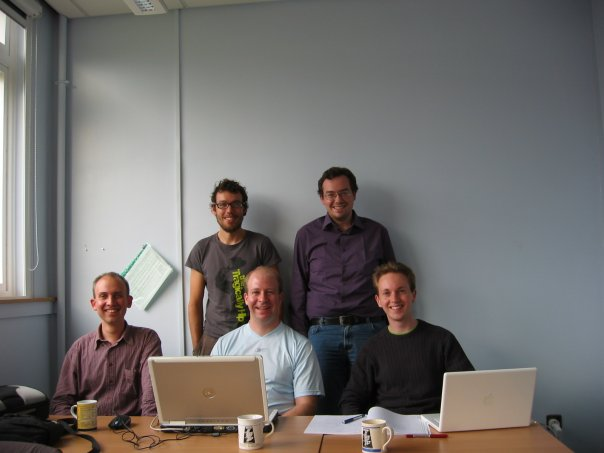
\includegraphics[scale=0.6]{./graphics/devteamstasep08.jpg}

 The development team meeting again (without Anton and Max), now in Vicenza in
april 2011. from left to right: Michel Lavrauw, John Bamberg, Philippe Cara,
Jan De Beule.

  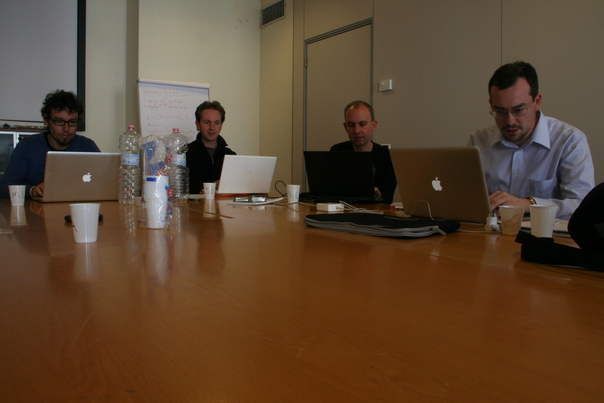
\includegraphics[scale=0.6]{./graphics/devteamvicapr11.jpg}

 Survivors of the first version of \textsf{FinInG}, enjoying a trip to Chioggia, december 2011. 

  
\includegraphics[scale=0.6]{./graphics/devteamchidec11.jpg}

 The same survivors, staring at the destiny. 

  
\includegraphics[scale=0.6]{./graphics/devteamdestiny.jpg}

 Anton Betten, during a milestone meeting at the finite geometries conference
in Irsee, september 2014. 

  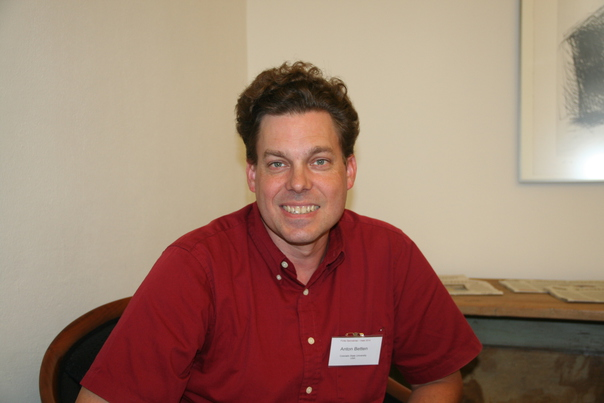
\includegraphics[scale=0.6]{./graphics/anton_irsee2014}

 }

  }

  
\chapter{\textcolor{Chapter }{Examples}}\label{examples}
\logpage{[ 2, 0, 0 ]}
\hyperdef{L}{X7A489A5D79DA9E5C}{}
{
  In this chapter we provide some simple examples of the use of \textsf{FinInG}. 
\section{\textcolor{Chapter }{Elementary examples}}\logpage{[ 2, 1, 0 ]}
\hyperdef{L}{X81660CB279889CB6}{}
{
  
\subsection{\textcolor{Chapter }{subspaces of projective spaces}}\logpage{[ 2, 1, 1 ]}
\hyperdef{L}{X8016E6857D53F2ED}{}
{


 The following example shows how to create some subspaces of a projective
space, test their incidence, and determine their span and intersection.
Projective spaces are considered as incidence geometries too. Incidence, to be
tested with \texttt{IsIncident} or equivalently \texttt{\texttt{\symbol{92}}*}, is symmetrized set-theoretic containment, the latter which can be tested
through the operation \texttt{in}. 
\begin{Verbatim}[commandchars=!@|,fontsize=\small,frame=single,label=Example]
  !gapprompt@gap>| !gapinput@pg := PG(3,8);|
  ProjectiveSpace(3, 8)
  !gapprompt@gap>| !gapinput@vec := [0,1,0,1]*Z(8)^0;|
  [ 0*Z(2), Z(2)^0, 0*Z(2), Z(2)^0 ]
  !gapprompt@gap>| !gapinput@point := VectorSpaceToElement(pg,vec);|
  <a point in ProjectiveSpace(3, 8)>
  !gapprompt@gap>| !gapinput@mat := [[0,0,1,1],[0,1,0,0]]*Z(8)^0;|
  [ [ 0*Z(2), 0*Z(2), Z(2)^0, Z(2)^0 ], [ 0*Z(2), Z(2)^0, 0*Z(2), 0*Z(2) ] ]
  !gapprompt@gap>| !gapinput@line := VectorSpaceToElement(pg,mat);|
  <a line in ProjectiveSpace(3, 8)>
  !gapprompt@gap>| !gapinput@mat2 := [[1,0,0,1],[1,0,1,0],[1,1,0,0]]*Z(8)^0;|
  [ [ Z(2)^0, 0*Z(2), 0*Z(2), Z(2)^0 ], [ Z(2)^0, 0*Z(2), Z(2)^0, 0*Z(2) ], 
    [ Z(2)^0, Z(2)^0, 0*Z(2), 0*Z(2) ] ]
  !gapprompt@gap>| !gapinput@plane := VectorSpaceToElement(pg,mat2);|
  <a plane in ProjectiveSpace(3, 8)>
  !gapprompt@gap>| !gapinput@IsIncident(point,line);|
  false
  !gapprompt@gap>| !gapinput@IsIncident(line,point);|
  false
  !gapprompt@gap>| !gapinput@point * line;|
  false
  !gapprompt@gap>| !gapinput@line * point|
  !gapprompt@>| !gapinput@point in line;|
  Syntax error: ; expected
  point in line;
      ^
  !gapprompt@gap>| !gapinput@line in point;|
  false
  !gapprompt@gap>| !gapinput@IsIncident(point,plane);|
  true
  !gapprompt@gap>| !gapinput@IsIncident(line,plane);|
  false
  !gapprompt@gap>| !gapinput@line in plane;|
  false
  !gapprompt@gap>| !gapinput@plane2 := Span(point,line);|
  <a plane in ProjectiveSpace(3, 8)>
  !gapprompt@gap>| !gapinput@Meet(plane,plane2);|
  <a line in ProjectiveSpace(3, 8)>
  !gapprompt@gap>| !gapinput@mat3 := [[1,0,0,0],[0,0,0,1]]*Z(8)^0;|
  [ [ Z(2)^0, 0*Z(2), 0*Z(2), 0*Z(2) ], [ 0*Z(2), 0*Z(2), 0*Z(2), Z(2)^0 ] ]
  !gapprompt@gap>| !gapinput@line2 := VectorSpaceToElement(pg,mat3);|
  <a line in ProjectiveSpace(3, 8)>
  !gapprompt@gap>| !gapinput@Meet(line,line2);|
  < empty subspace >
  !gapprompt@gap>| !gapinput@Span(plane,plane2);|
  ProjectiveSpace(3, 8)
  
\end{Verbatim}
 }

 
\subsection{\textcolor{Chapter }{Subspaces of classical polar spaces}}\logpage{[ 2, 1, 2 ]}
\hyperdef{L}{X7B99511887D41A95}{}
{


 \textsf{FinInG} provides classical polar spaces. Subspaces can be constructed the same way as
subspaces of projective spaces. Upon construction, it is checked whether the
given vector space does determine a subspace of the polar space. Subspaces of
polar spaces are also subspaces of the ambient projective space. Operations
like \texttt{Span} and \texttt{Meet} are naturally applicable. However, the span of two subspaces might not be a
subspace of the polar space anymore, and if the two subspaces belong to two
different polar spaces in the same ambient projective space, it cannot be
determined in which polar space the span should be constructed. Therefore the
result of \texttt{Span} of two subspaces of a polar space is a subspace of the ambient projective
space. It can be checked whether the result belongs to a polar space using \texttt{in}. This illustrates very well a general philosophy: a subspace of a polar
space, and more generally, an element of any incidence structure is always
aware of its ambient geometry. This example also illustrates how to create an
element that belongs to the polar space from the subspace of the ambient
projective geometry by using \texttt{ElementToElement}. Finally note the behaviour of \texttt{=} applied on the two subspaces. Clearly, a subspace of a polar space is really
also a subspace of the ambient projective space. 
\begin{Verbatim}[commandchars=!@|,fontsize=\small,frame=single,label=Example]
  !gapprompt@gap>| !gapinput@ps := EllipticQuadric(5,7);|
  Q-(5, 7)
  !gapprompt@gap>| !gapinput@vec := [1,0,0,0,0,0]*Z(7)^0;|
  [ Z(7)^0, 0*Z(7), 0*Z(7), 0*Z(7), 0*Z(7), 0*Z(7) ]
  !gapprompt@gap>| !gapinput@point := VectorSpaceToElement(ps,vec);|
  Error, <v> does not generate an element of <geom> called from
  <function "unknown">( <arguments> )
   called from read-eval loop at line 10 of *stdin*
  you can 'quit;' to quit to outer loop, or
  you can 'return;' to continue
  !gapbrkprompt@brk>| !gapinput@quit;|
  !gapprompt@gap>| !gapinput@EquationForPolarSpace(ps);|
  x_1^2+x_2^2+x_3*x_4+x_5*x_6
  !gapprompt@gap>| !gapinput@vec := [0,0,1,0,0,0]*Z(7)^0;|
  [ 0*Z(7), 0*Z(7), Z(7)^0, 0*Z(7), 0*Z(7), 0*Z(7) ]
  !gapprompt@gap>| !gapinput@point := VectorSpaceToElement(ps,vec);|
  <a point in Q-(5, 7)>
  !gapprompt@gap>| !gapinput@vec2 := [0,0,0,1,0,0]*Z(7)^0;|
  [ 0*Z(7), 0*Z(7), 0*Z(7), Z(7)^0, 0*Z(7), 0*Z(7) ]
  !gapprompt@gap>| !gapinput@point2 := VectorSpaceToElement(ps,vec2);|
  <a point in Q-(5, 7)>
  !gapprompt@gap>| !gapinput@line := Span(point,point2);|
  <a line in ProjectiveSpace(5, 7)>
  !gapprompt@gap>| !gapinput@mat := [[0,0,1,0,0,0],[0,0,0,0,1,0]]*Z(7)^0;|
  [ [ 0*Z(7), 0*Z(7), Z(7)^0, 0*Z(7), 0*Z(7), 0*Z(7) ], 
    [ 0*Z(7), 0*Z(7), 0*Z(7), 0*Z(7), Z(7)^0, 0*Z(7) ] ]
  !gapprompt@gap>| !gapinput@line2 := VectorSpaceToElement(ps,mat);|
  <a line in Q-(5, 7)>
  !gapprompt@gap>| !gapinput@meet := Meet(line,line2);|
  <a point in ProjectiveSpace(5, 7)>
  !gapprompt@gap>| !gapinput@meet in ps;|
  true
  !gapprompt@gap>| !gapinput@point3 := ElementToElement(ps,meet);|
  <a point in Q-(5, 7)>
  
\end{Verbatim}
 }

 
\subsection{\textcolor{Chapter }{Underlying objects}}\logpage{[ 2, 1, 3 ]}
\hyperdef{L}{X8555398C83677C27}{}
{


 Subspaces of projective spaces and polar spaces (and in general, elements of
incidence structures), are determined by a mathematical object, called in \textsf{FinInG} the \emph{underlying object}. The operation \texttt{UnderlyingObject} simply returns this underlying object. For elements determined by vectors or
sub vector spaces, the underlying objects are a vector or a matrix. To
represent these objects and to do very efficient orbit calculations under
groups, we use the \textsf{cvec}. This can be noted when applying \texttt{UnderlyingObject}. The operation \texttt{Unpack} simply converts the cvec objects into GAP vectors and matrices. The example
also illustrates how the underlying object of an element of an affine spaces
looks like. 
\begin{Verbatim}[commandchars=!@|,fontsize=\small,frame=single,label=Example]
  !gapprompt@gap>| !gapinput@pg := PG(3,169);|
  ProjectiveSpace(3, 169)
  !gapprompt@gap>| !gapinput@p := Random(Points(pg));|
  <a point in ProjectiveSpace(3, 169)>
  !gapprompt@gap>| !gapinput@UnderlyingObject(p);|
  <cvec over GF(13,2) of length 4>
  !gapprompt@gap>| !gapinput@Unpack(last);|
  [ Z(13)^0, Z(13^2)^49, Z(13^2)^31, Z(13^2)^143 ]
  !gapprompt@gap>| !gapinput@l := Random(Lines(pg));|
  <a line in ProjectiveSpace(3, 169)>
  !gapprompt@gap>| !gapinput@UnderlyingObject(l);|
  <cmat 2x4 over GF(13,2)>
  !gapprompt@gap>| !gapinput@Unpack(last);|
  [ [ Z(13)^0, 0*Z(13), 0*Z(13), Z(13^2)^96 ], 
    [ 0*Z(13), Z(13)^0, Z(13^2)^113, Z(13^2)^99 ] ]
  !gapprompt@gap>| !gapinput@quadric := EllipticQuadric(5,2);|
  Q-(5, 2)
  !gapprompt@gap>| !gapinput@line := Random(Lines(quadric));|
  <a line in Q-(5, 2)>
  !gapprompt@gap>| !gapinput@UnderlyingObject(line);|
  <cmat 2x6 over GF(2,1)>
  !gapprompt@gap>| !gapinput@Unpack(last);|
  [ [ 0*Z(2), 0*Z(2), Z(2)^0, 0*Z(2), 0*Z(2), Z(2)^0 ], 
    [ 0*Z(2), 0*Z(2), 0*Z(2), Z(2)^0, Z(2)^0, 0*Z(2) ] ]
  !gapprompt@gap>| !gapinput@ag := AG(4,3);|
  AG(4, 3)
  !gapprompt@gap>| !gapinput@plane := Random(Planes(ag));|
  <a plane in AG(4, 3)>
  !gapprompt@gap>| !gapinput@UnderlyingObject(plane);|
  [ <cvec over GF(3,1) of length 4>, <cmat 2x4 over GF(3,1)> ]
  
\end{Verbatim}
 }

 
\subsection{\textcolor{Chapter }{Constructing polar spaces}}\logpage{[ 2, 1, 4 ]}
\hyperdef{L}{X8771ACB879E479C6}{}
{


 \textsf{FinInG} provides the classical polar spaces as the geometries of which the subspaces
are represented by the totally isotropic (resp. totally singular) vector
subspaces with relation to a chosen sesquilinear (resp. quadratic form). The
user may choose any non-degenerate (resp. non-singular) form to construct the
polar space. The usage of the forms makes \textsf{FinInG} dependent on the package \textsf{forms}. Shortcuts to polar spaces in \emph{standard} representation are included. Detailed information can be found in Section \ref{can_standard}. 
\begin{Verbatim}[commandchars=!@|,fontsize=\small,frame=single,label=Example]
  !gapprompt@gap>| !gapinput@ps := HermitianPolarSpace(4,9);|
  H(4, 3^2)
  !gapprompt@gap>| !gapinput@EquationForPolarSpace(ps);|
  x_1^4+x_2^4+x_3^4+x_4^4+x_5^4
  !gapprompt@gap>| !gapinput@ps := HyperbolicQuadric(5,7);|
  Q+(5, 7)
  !gapprompt@gap>| !gapinput@EquationForPolarSpace(ps);|
  x_1*x_2+x_3*x_4+x_5*x_6
  !gapprompt@gap>| !gapinput@ps := SymplecticSpace(3,3);|
  W(3, 3)
  !gapprompt@gap>| !gapinput@EquationForPolarSpace(ps);|
  x1*y2-x2*y1+x3*y4-x4*y3
  !gapprompt@gap>| !gapinput@mat := IdentityMat(4,GF(11));|
  [ [ Z(11)^0, 0*Z(11), 0*Z(11), 0*Z(11) ], 
    [ 0*Z(11), Z(11)^0, 0*Z(11), 0*Z(11) ], 
    [ 0*Z(11), 0*Z(11), Z(11)^0, 0*Z(11) ], 
    [ 0*Z(11), 0*Z(11), 0*Z(11), Z(11)^0 ] ]
  !gapprompt@gap>| !gapinput@form := BilinearFormByMatrix(mat,GF(11));|
  < bilinear form >
  !gapprompt@gap>| !gapinput@ps := PolarSpace(form);|
  <polar space in ProjectiveSpace(3,GF(11)): x_1^2+x_2^2+x_3^2+x_4^2=0 >
  !gapprompt@gap>| !gapinput@Rank(ps);|
  2
  !gapprompt@gap>| !gapinput@ps;|
  Q+(3, 11): x_1^2+x_2^2+x_3^2+x_4^2=0
  
\end{Verbatim}
 }

 
\subsection{\textcolor{Chapter }{Some collineation groups}}\logpage{[ 2, 1, 5 ]}
\hyperdef{L}{X85D3BB2A8274DDCB}{}
{


 In principle, the full group of collineations of almost any incidence
structure can be computed in \textsf{FinInG}. Mathematically, this is almost obvious for projective spaces and affine
spaces. For classical polar spaces, the particular forms plays a role. The
coordinate change capabilities of the package \textsf{forms}, together with the standard theory (see \cite{KleidmanLiebeck}), ensure that the full collineation group of a classical polar space can be
relatively easily obtained. The computation of the full collineation group of
particular incidence structures, such as generalised polygons, may rely on the
computation of the automorphism group of an underlying incidence graph, which
is done by using nauty through the package \textsf{GRAPE}. Note that the elements of a projective collineation group are semilinear
maps, they consist of a matrix together with a field automorphism. 
\begin{Verbatim}[commandchars=!@|,fontsize=\small,frame=single,label=Example]
  !gapprompt@gap>| !gapinput@pg := PG(3,4);|
  ProjectiveSpace(3, 4)
  !gapprompt@gap>| !gapinput@coll := CollineationGroup(pg);|
  The FinInG collineation group PGammaL(4,4)
  !gapprompt@gap>| !gapinput@gens := GeneratorsOfGroup(coll);|
  [ < a collineation: <cmat 4x4 over GF(2,2)>, F^0>, 
    < a collineation: <cmat 4x4 over GF(2,2)>, F^0>, 
    < a collineation: <cmat 4x4 over GF(2,2)>, F^2> ]
  !gapprompt@gap>| !gapinput@UnderlyingMatrix(gens[2]);|
  <cmat 4x4 over GF(2,2)>
  !gapprompt@gap>| !gapinput@Unpack(last);|
  [ [ Z(2)^0, 0*Z(2), 0*Z(2), Z(2)^0 ], [ Z(2)^0, 0*Z(2), 0*Z(2), 0*Z(2) ], 
    [ 0*Z(2), Z(2)^0, 0*Z(2), 0*Z(2) ], [ 0*Z(2), 0*Z(2), Z(2)^0, 0*Z(2) ] ]
  !gapprompt@gap>| !gapinput@as := AffineSpace(3,4);|
  AG(3, 4)
  !gapprompt@gap>| !gapinput@coll := CollineationGroup(as);|
  AGammaL(3,4)
  !gapprompt@gap>| !gapinput@GeneratorsOfGroup(coll);|
  [ < a collineation: <cmat 4x4 over GF(2,2)>, F^0>, 
    < a collineation: <cmat 4x4 over GF(2,2)>, F^0>, 
    < a collineation: <cmat 4x4 over GF(2,2)>, F^0>, 
    < a collineation: <cmat 4x4 over GF(2,2)>, F^2> ]
  !gapprompt@gap>| !gapinput@gp := SplitCayleyHexagon(3);|
  H(3)
  !gapprompt@gap>| !gapinput@coll:= CollineationGroup(gp);|
  #I  for Split Cayley Hexagon
  #I  Computing nice monomorphism...
  #I  Found permutation domain...
  G_2(3)
  !gapprompt@gap>| !gapinput@GeneratorsOfGroup(coll);|
  [ < a collineation: <cmat 7x7 over GF(3,1)>, F^0>, 
    < a collineation: <cmat 7x7 over GF(3,1)>, F^0>, 
    < a collineation: <cmat 7x7 over GF(3,1)>, F^0>, 
    < a collineation: <cmat 7x7 over GF(3,1)>, F^0>, 
    < a collineation: <cmat 7x7 over GF(3,1)>, F^0> ]
  !gapprompt@gap>| !gapinput@egq := EGQByqClan(LinearqClan(3));|
  #I  Computed Kantor family. Now computing EGQ...
  <EGQ of order [ 9, 3 ] and basepoint 0>
  !gapprompt@gap>| !gapinput@coll := CollineationGroup(egq);|
  #I  Computing incidence graph of generalised polygon...
  #I  Using elation of the collineation group...
  <permutation group of size 26127360 with 6 generators>
  
\end{Verbatim}
 }

 }

 
\section{\textcolor{Chapter }{Some objects with interesting combinatorial properties}}\logpage{[ 2, 2, 0 ]}
\hyperdef{L}{X825F78F57E309197}{}
{
  The examples here are meant to give a flavour of how to explore geometrical
objects from different point of views. 
\subsection{\textcolor{Chapter }{The Tits ovoid}}\logpage{[ 2, 2, 1 ]}
\hyperdef{L}{X815BB30986E84DB1}{}
{


 In this example we consider the Tits ovoid in $PG(3,8)$. We explicitly check the intersection number of the Tits-ovoid with planes of
the projective space, and compute its stabiliser group inside the homography
group of $PG(3,8)$. The use of \texttt{;;} after a command suppresses its output, which is particularly interesting if
the output is a long list. The operation \texttt{Collected} is self-explanatory, and a very useful GAP command. The computed stabiliser is
the Suzuki group $Sz(8)$, a finite simple group. 
\begin{Verbatim}[commandchars=!@|,fontsize=\small,frame=single,label=Example]
  !gapprompt@gap>| !gapinput@q := 8;|
  8
  !gapprompt@gap>| !gapinput@pg := PG(3,q);|
  ProjectiveSpace(3, 8)
  !gapprompt@gap>| !gapinput@f := GF(q);|
  GF(2^3)
  !gapprompt@gap>| !gapinput@vecs := Union(List(f,x->List(f,y->[One(f),x*y+x^6+y^4,x,y])));;|
  !gapprompt@gap>| !gapinput@Add(vecs,[0,1,0,0]*Z(q)^0);|
  !gapprompt@gap>| !gapinput@ovoid := List(vecs,x->VectorSpaceToElement(pg,x));;|
  !gapprompt@gap>| !gapinput@numbers := List(Planes(pg),x->Number(ovoid,y->y in x));|
  [ 9, 9, 9, 9, 9, 9, 9, 9, 9, 9, 9, 9, 9, 9, 9, 9, 9, 9, 9, 9, 9, 9, 9, 9, 9, 
    9, 9, 9, 9, 9, 9, 9, 9, 9, 9, 9, 9, 9, 9, 9, 9, 9, 9, 9, 9, 9, 9, 9, 9, 9, 
    9, 9, 9, 9, 9, 9, 9, 9, 9, 9, 9, 9, 9, 9, 9, 9, 9, 9, 9, 9, 9, 9, 1, 1, 9, 
    9, 9, 9, 9, 9, 9, 9, 9, 1, 9, 9, 1, 9, 9, 9, 9, 9, 1, 1, 9, 9, 9, 9, 9, 9, 
    9, 9, 9, 9, 9, 9, 1, 9, 9, 9, 9, 1, 9, 9, 9, 9, 9, 9, 9, 9, 9, 9, 9, 9, 9, 
    9, 9, 9, 9, 9, 9, 9, 9, 9, 9, 9, 9, 9, 9, 9, 9, 9, 9, 9, 9, 9, 9, 9, 9, 1, 
    9, 1, 9, 9, 9, 9, 9, 9, 9, 9, 9, 9, 9, 9, 9, 9, 9, 9, 1, 9, 9, 9, 9, 9, 1, 
    9, 9, 1, 9, 9, 1, 9, 9, 9, 9, 9, 1, 1, 9, 9, 9, 9, 9, 9, 9, 9, 9, 9, 9, 9, 
    9, 9, 9, 9, 9, 9, 9, 9, 1, 9, 9, 9, 1, 9, 9, 9, 9, 9, 1, 9, 9, 9, 1, 9, 9, 
    1, 9, 9, 9, 9, 9, 1, 9, 9, 9, 9, 9, 9, 9, 9, 9, 9, 9, 1, 9, 1, 9, 9, 9, 9, 
    9, 9, 9, 9, 9, 9, 9, 9, 9, 9, 9, 9, 9, 9, 9, 9, 9, 9, 9, 1, 1, 9, 9, 9, 9, 
    9, 9, 9, 9, 9, 9, 1, 9, 1, 9, 9, 9, 9, 9, 9, 9, 9, 9, 9, 9, 9, 9, 9, 9, 9, 
    9, 9, 9, 9, 1, 9, 1, 9, 9, 9, 9, 9, 9, 9, 9, 9, 1, 9, 9, 1, 9, 9, 9, 9, 9, 
    9, 9, 9, 9, 9, 9, 9, 9, 9, 9, 9, 9, 9, 9, 9, 9, 9, 9, 9, 1, 9, 9, 9, 9, 9, 
    9, 1, 9, 9, 1, 9, 9, 1, 9, 9, 9, 9, 9, 1, 1, 9, 9, 9, 9, 9, 9, 9, 9, 9, 9, 
    9, 9, 1, 9, 9, 9, 9, 1, 9, 9, 9, 9, 9, 9, 9, 9, 9, 9, 9, 9, 1, 9, 9, 9, 1, 
    9, 1, 1, 9, 9, 9, 9, 9, 9, 9, 9, 9, 9, 9, 9, 9, 9, 9, 9, 9, 1, 9, 1, 9, 9, 
    9, 9, 9, 9, 9, 9, 9, 9, 9, 9, 9, 9, 9, 9, 9, 1, 9, 9, 9, 9, 1, 9, 9, 9, 9, 
    9, 9, 9, 9, 9, 9, 9, 9, 1, 9, 1, 9, 9, 9, 9, 9, 9, 9, 9, 9, 9, 9, 9, 9, 9, 
    9, 9, 9, 9, 9, 1, 9, 9, 1, 9, 9, 9, 9, 9, 1, 9, 9, 9, 1, 9, 9, 9, 9, 9, 9, 
    9, 9, 1, 1, 9, 9, 9, 9, 9, 9, 9, 9, 9, 9, 9, 9, 9, 9, 9, 9, 9, 1, 9, 9, 9, 
    9, 9, 9, 9, 9, 9, 1, 9, 9, 9, 9, 9, 9, 9, 9, 9, 1, 9, 9, 9, 9, 9, 9, 9, 9, 
    9, 1, 9, 9, 1, 9, 9, 9, 9, 9, 9, 9, 9, 9, 1, 9, 9, 9, 9, 9, 9, 9, 9, 9, 1, 
    9, 1, 9, 9, 9, 9, 9, 9, 9, 1 ]
  !gapprompt@gap>| !gapinput@Collected(numbers);|
  [ [ 1, 65 ], [ 9, 520 ] ]
  !gapprompt@gap>| !gapinput@group := HomographyGroup(pg);|
  The FinInG projectivity group PGL(4,8)
  !gapprompt@gap>| !gapinput@stab := FiningSetwiseStabiliser(group,ovoid);|
  #I  Computing adjusted stabilizer chain...
  <projective collineation group with 5 generators>
  !gapprompt@gap>| !gapinput@time;|
  55290
  !gapprompt@gap>| !gapinput@IsSimple(stab);|
  true
  !gapprompt@gap>| !gapinput@Order(stab);|
  29120
  
\end{Verbatim}
 }

 
\subsection{\textcolor{Chapter }{Lines meeting a hermitian curve}}\logpage{[ 2, 2, 2 ]}
\hyperdef{L}{X7E79F18B8170B4B3}{}
{


 Here we see how the lines of a projective plane $PG(2,q^2)$  meet a hermitian curve. It is well known that every line meets in either 1 or $q+1$ points. Note that the last comment takes a while to complete. 
\begin{Verbatim}[commandchars=!@|,fontsize=\small,frame=single,label=Example]
  !gapprompt@gap>| !gapinput@h:=HermitianPolarSpace(2, 7^2);|
  H(2, 7^2)
  !gapprompt@gap>| !gapinput@pg := AmbientSpace( h );|
  ProjectiveSpace(2, 49)
  !gapprompt@gap>| !gapinput@lines := Lines( pg );|
  <lines of ProjectiveSpace(2, 49)>
  !gapprompt@gap>| !gapinput@curve := AsList( Points( h ) );;|
  !gapprompt@gap>| !gapinput@Size(curve);|
  344
  !gapprompt@gap>| !gapinput@Collected( List(lines, t -> Number(curve, c-> c in t)));|
  [ [ 1, 344 ], [ 8, 2107 ] ]
  !gapprompt@gap>| !gapinput@time;|
  26412
   
\end{Verbatim}
 }

 
\subsection{\textcolor{Chapter }{The Patterson ovoid}}\logpage{[ 2, 2, 3 ]}
\hyperdef{L}{X85C255FD78C50992}{}
{


 In this example, we construct the unique ovoid of the parabolic quadric $Q(6,3)$, first discovered by Patterson, but for which was given a nice construction
by E. E. Shult. We begin with the ``sums of squares'' quadratic form over $GF(3)$ and the associated polar space. 
\begin{Verbatim}[commandchars=!@|,fontsize=\small,frame=single,label=Example]
  !gapprompt@gap>| !gapinput@id := IdentityMat(7, GF(3));;|
  !gapprompt@gap>| !gapinput@form := QuadraticFormByMatrix(id, GF(3));|
  < quadratic form >
  !gapprompt@gap>| !gapinput@ps := PolarSpace( form );|
  <polar space in ProjectiveSpace(
  6,GF(3)): x_1^2+x_2^2+x_3^2+x_4^2+x_5^2+x_6^2+x_7^2=0 >
\end{Verbatim}
 The construction of the ovoid (a la Shult): 
\begin{Verbatim}[commandchars=!@|,fontsize=\small,frame=single,label=Example]
  !gapprompt@gap>| !gapinput@psl32 := PSL(3,2);|
  Group([ (4,6)(5,7), (1,2,4)(3,6,5) ])
  !gapprompt@gap>| !gapinput@reps:=[[1,1,1,0,0,0,0], [-1,1,1,0,0,0,0],|
  !gapprompt@>| !gapinput@[1,-1,1,0,0,0,0], [1,1,-1,0,0,0,0]]*Z(3)^0;|
  [ [ Z(3)^0, Z(3)^0, Z(3)^0, 0*Z(3), 0*Z(3), 0*Z(3), 0*Z(3) ], 
    [ Z(3), Z(3)^0, Z(3)^0, 0*Z(3), 0*Z(3), 0*Z(3), 0*Z(3) ], 
    [ Z(3)^0, Z(3), Z(3)^0, 0*Z(3), 0*Z(3), 0*Z(3), 0*Z(3) ], 
    [ Z(3)^0, Z(3)^0, Z(3), 0*Z(3), 0*Z(3), 0*Z(3), 0*Z(3) ] ]
  !gapprompt@gap>| !gapinput@ovoid := Union( List(reps, x-> Orbit(psl32, x, Permuted)) );;|
  !gapprompt@gap>| !gapinput@ovoid := List(ovoid, x -> VectorSpaceToElement(ps, x));;|
\end{Verbatim}
 We check that this is indeed an ovoid. The observant reader will notice \emph{\#I Computing collineation group of canonical polar space...} which is caused by the command \texttt{AsList} applied to the collection of elements \mbox{\texttt{\mdseries\slshape planes}}. The use of \texttt{AsList} invokes the computation of all elements in \mbox{\texttt{\mdseries\slshape planes}} as an orbit under the collineation group of the ambient polar space. The
reader is invited to redo, in a new GAP session, the same example omitting the \texttt{AsList} command, just defining \texttt{planes := Planes(ps);;}. The result will be te same, but the computation of all elements will now be
done using an enumerator, and will be slower. 
\begin{Verbatim}[commandchars=!@|,fontsize=\small,frame=single,label=Example]
  !gapprompt@gap>| !gapinput@planes := AsList(Planes( ps ));;|
  #I  Computing collineation group of canonical polar space...
  !gapprompt@gap>| !gapinput@ForAll(planes, p -> Number(ovoid, x -> x * p) = 1);|
  true
\end{Verbatim}
 The stabiliser is interesting since it yields the embedding of $Sp(6,2)$ in $PO(7,3)$. To efficiently compute the set-wise stabiliser, we refer to the induced
permutation representation. 
\begin{Verbatim}[commandchars=!@A,fontsize=\small,frame=single,label=Example]
  !gapprompt@gap>A !gapinput@g := IsometryGroup( ps );A
  #I  Computing collineation group of canonical polar space...
  <projective collineation group of size 9170703360 with 2 generators>
  !gapprompt@gap>A !gapinput@stabovoid := FiningSetwiseStabiliser(g, ovoid);A
  #I  Computing adjusted stabilizer chain...
  <projective collineation group with 13 generators>
  !gapprompt@gap>A !gapinput@DisplayCompositionSeries(stabovoid);A
  G (size 1451520)
   | B(3,2) = O(7,2) ~ C(3,2) = S(6,2)
  1 (size 1)
  !gapprompt@gap>A !gapinput@OrbitLengths(stabovoid, ovoid);A
  [ 28 ]
  !gapprompt@gap>A !gapinput@IsTransitive(stabovoid, ovoid);A
  true 
\end{Verbatim}
 }

 
\subsection{\textcolor{Chapter }{A hyperoval}}\logpage{[ 2, 2, 4 ]}
\hyperdef{L}{X80B93785876EF3E0}{}
{


 In this example, we consider a hyperoval of the projective plane $PG(2,4)$, that is, six points no three collinear. We will construct such a hyperoval
by some basic explorations into particular properties of the projective plane $PG(2,4)$. The projective plane is initialised, its points are computed and listed;
then a standard frame is constructed, of which we may assume that it is a
subset of the hyperoval. Finally, the stabiliser group of the hyperoval is
computed, and it is checked that this group is isomorphic with the symmetric
group on six elements. 
\begin{Verbatim}[commandchars=!@|,fontsize=\small,frame=single,label=Example]
  !gapprompt@gap>| !gapinput@pg := ProjectiveSpace(2,4);|
  ProjectiveSpace(2, 4)
  !gapprompt@gap>| !gapinput@points := Points(pg);|
  <points of ProjectiveSpace(2, 4)>
  !gapprompt@gap>| !gapinput@pointslist := AsList(points);|
  [ <a point in ProjectiveSpace(2, 4)>, <a point in ProjectiveSpace(2, 4)>, 
    <a point in ProjectiveSpace(2, 4)>, <a point in ProjectiveSpace(2, 4)>, 
    <a point in ProjectiveSpace(2, 4)>, <a point in ProjectiveSpace(2, 4)>, 
    <a point in ProjectiveSpace(2, 4)>, <a point in ProjectiveSpace(2, 4)>, 
    <a point in ProjectiveSpace(2, 4)>, <a point in ProjectiveSpace(2, 4)>, 
    <a point in ProjectiveSpace(2, 4)>, <a point in ProjectiveSpace(2, 4)>, 
    <a point in ProjectiveSpace(2, 4)>, <a point in ProjectiveSpace(2, 4)>, 
    <a point in ProjectiveSpace(2, 4)>, <a point in ProjectiveSpace(2, 4)>, 
    <a point in ProjectiveSpace(2, 4)>, <a point in ProjectiveSpace(2, 4)>, 
    <a point in ProjectiveSpace(2, 4)>, <a point in ProjectiveSpace(2, 4)>, 
    <a point in ProjectiveSpace(2, 4)> ]
  !gapprompt@gap>| !gapinput@Display(pointslist[1]);|
   . . 1
\end{Verbatim}
 Now we may assume that our hyperoval contains the fundamental frame. 
\begin{Verbatim}[commandchars=!@|,fontsize=\small,frame=single,label=Example]
  !gapprompt@gap>| !gapinput@frame := [[1,0,0],[0,1,0],[0,0,1],[1,1,1]]*Z(2)^0;|
  [ [ Z(2)^0, 0*Z(2), 0*Z(2) ], [ 0*Z(2), Z(2)^0, 0*Z(2) ], 
    [ 0*Z(2), 0*Z(2), Z(2)^0 ], [ Z(2)^0, Z(2)^0, Z(2)^0 ] ]
  !gapprompt@gap>| !gapinput@frame := List(frame,x -> VectorSpaceToElement(pg,x));|
  [ <a point in ProjectiveSpace(2, 4)>, <a point in ProjectiveSpace(2, 4)>, 
    <a point in ProjectiveSpace(2, 4)>, <a point in ProjectiveSpace(2, 4)> ]
\end{Verbatim}
 Alternatively, we could use: 
\begin{Verbatim}[commandchars=!@|,fontsize=\small,frame=single,label=Example]
  !gapprompt@gap>| !gapinput@frame := StandardFrame( pg );|
  [ <a point in ProjectiveSpace(2, 4)>, <a point in ProjectiveSpace(2, 4)>, 
    <a point in ProjectiveSpace(2, 4)>, <a point in ProjectiveSpace(2, 4)> ]
\end{Verbatim}
 There are six secant lines to this frame (``four choose two''). So we put
together these secant lines from the pairs of points of this frame. 
\begin{Verbatim}[commandchars=!@|,fontsize=\small,frame=single,label=Example]
  !gapprompt@gap>| !gapinput@pairs := Combinations(frame,2);|
  [ [ <a point in ProjectiveSpace(2, 4)>, <a point in ProjectiveSpace(2, 4)> ], 
    [ <a point in ProjectiveSpace(2, 4)>, <a point in ProjectiveSpace(2, 4)> ], 
    [ <a point in ProjectiveSpace(2, 4)>, <a point in ProjectiveSpace(2, 4)> ], 
    [ <a point in ProjectiveSpace(2, 4)>, <a point in ProjectiveSpace(2, 4)> ], 
    [ <a point in ProjectiveSpace(2, 4)>, <a point in ProjectiveSpace(2, 4)> ], 
    [ <a point in ProjectiveSpace(2, 4)>, <a point in ProjectiveSpace(2, 4)> ] ]
  !gapprompt@gap>| !gapinput@secants := List(pairs,p -> Span(p[1],p[2]));|
  [ <a line in ProjectiveSpace(2, 4)>, <a line in ProjectiveSpace(2, 4)>, 
    <a line in ProjectiveSpace(2, 4)>, <a line in ProjectiveSpace(2, 4)>, 
    <a line in ProjectiveSpace(2, 4)>, <a line in ProjectiveSpace(2, 4)> ]
\end{Verbatim}
 By a counting argument, it is known that the frame of $PG(2,4)$ completes uniquely to a hyperoval. 
\begin{Verbatim}[commandchars=!@|,fontsize=\small,frame=single,label=Example]
  !gapprompt@gap>| !gapinput@leftover := Filtered(pointslist,t->not ForAny(secants,s->t in s));|
  [ <a point in ProjectiveSpace(2, 4)>, <a point in ProjectiveSpace(2, 4)> ]
  !gapprompt@gap>| !gapinput@hyperoval := Union(frame,leftover);|
  [ <a point in ProjectiveSpace(2, 4)>, <a point in ProjectiveSpace(2, 4)>, 
    <a point in ProjectiveSpace(2, 4)>, <a point in ProjectiveSpace(2, 4)>, 
    <a point in ProjectiveSpace(2, 4)>, <a point in ProjectiveSpace(2, 4)> ]
\end{Verbatim}
 This hyperoval has the symmetric group on six symbols as its stabiliser, which
can easily be calculated: 
\begin{Verbatim}[commandchars=!@|,fontsize=\small,frame=single,label=Example]
  !gapprompt@gap>| !gapinput@g := CollineationGroup(pg);|
  The FinInG collineation group PGammaL(3,4)
  !gapprompt@gap>| !gapinput@stab := Stabilizer(g,Set(hyperoval),OnSets);|
  <projective collineation group of size 720>
  !gapprompt@gap>| !gapinput@StructureDescription(stab);|
  "S6" 
\end{Verbatim}
 }

 }

 
\section{\textcolor{Chapter }{Geometry morphisms}}\logpage{[ 2, 3, 0 ]}
\hyperdef{L}{X876240A479A5717C}{}
{
  A geometry morphism in \textsf{FinInG} is a map between (a subset of) the elements of one geometry to (a subset of)
the elements of a second geometry, preserving the incidence. Geometry
morphisms are not necessarily type preserving. This section is meant to
illustrate, in a non exhaustive way the basis philisophy behind geometry
morphisms in \textsf{FinInG}. 
\subsection{\textcolor{Chapter }{Isomorphic polar spaces}}\logpage{[ 2, 3, 1 ]}
\hyperdef{L}{X79CE092B7E17DF24}{}
{


 We've seen already that a polar space can be constructed from any
non-degenerate sesquilinear or non-singular quadratic form. An isomorphism
between polar spaces of the same type, can easily be obtained. This example
illustrates \texttt{IsomorphismPolarSpaces}, which is in its basic use self-explanatory, and the use of the obtained map
to compute images and pre-images of elements. 
\begin{Verbatim}[commandchars=!@|,fontsize=\small,frame=single,label=Example]
  !gapprompt@gap>| !gapinput@mat1 := IdentityMat(4,GF(16));|
  [ [ Z(2)^0, 0*Z(2), 0*Z(2), 0*Z(2) ], [ 0*Z(2), Z(2)^0, 0*Z(2), 0*Z(2) ], 
    [ 0*Z(2), 0*Z(2), Z(2)^0, 0*Z(2) ], [ 0*Z(2), 0*Z(2), 0*Z(2), Z(2)^0 ] ]
  !gapprompt@gap>| !gapinput@form1 := HermitianFormByMatrix(mat1,GF(16));|
  < hermitian form >
  !gapprompt@gap>| !gapinput@ps1 := PolarSpace(form1);|
  <polar space in ProjectiveSpace(3,GF(2^4)): x_1^5+x_2^5+x_3^5+x_4^5=0 >
  !gapprompt@gap>| !gapinput@mat2 := [[0,1,0,0],[1,0,0,0],[0,0,0,1],[0,0,1,0]]*Z(16)^0;|
  [ [ 0*Z(2), Z(2)^0, 0*Z(2), 0*Z(2) ], [ Z(2)^0, 0*Z(2), 0*Z(2), 0*Z(2) ], 
    [ 0*Z(2), 0*Z(2), 0*Z(2), Z(2)^0 ], [ 0*Z(2), 0*Z(2), Z(2)^0, 0*Z(2) ] ]
  !gapprompt@gap>| !gapinput@form2 := HermitianFormByMatrix(mat2,GF(16));|
  < hermitian form >
  !gapprompt@gap>| !gapinput@ps2 := PolarSpace(form2);|
  <polar space in ProjectiveSpace(
  3,GF(2^4)): x_1^4*x_2+x_1*x_2^4+x_3^4*x_4+x_3*x_4^4=0 >
  !gapprompt@gap>| !gapinput@map := IsomorphismPolarSpaces(ps1,ps2);|
  #I  No intertwiner computed. One of the polar spaces must have a collineation group computed
  <geometry morphism from <Elements of H(3, 
  4^2): x_1^5+x_2^5+x_3^5+x_4^5=0> to <Elements of H(3, 
  4^2): x_1^4*x_2+x_1*x_2^4+x_3^4*x_4+x_3*x_4^4=0>>
  !gapprompt@gap>| !gapinput@p := Random(Points(ps1));|
  <a point in H(3, 4^2): x_1^5+x_2^5+x_3^5+x_4^5=0>
  !gapprompt@gap>| !gapinput@p^map;|
  <a point in H(3, 4^2): x_1^4*x_2+x_1*x_2^4+x_3^4*x_4+x_3*x_4^4=0>
  !gapprompt@gap>| !gapinput@l := Random(Lines(ps2));|
  <a line in H(3, 4^2): x_1^4*x_2+x_1*x_2^4+x_3^4*x_4+x_3*x_4^4=0>
  !gapprompt@gap>| !gapinput@PreImageElm(map,l);|
  <a line in H(3, 4^2): x_1^5+x_2^5+x_3^5+x_4^5=0>
   
\end{Verbatim}
 }

 
\subsection{\textcolor{Chapter }{Intertwiners}}\logpage{[ 2, 3, 2 ]}
\hyperdef{L}{X83ADB5AE8624C74C}{}
{


 We reconsider the previous example. The observant reader might have noticed
the message \emph{\#I No intertwiner computed...}. Given a geometry morphism $f$ from $S$ to $S'$, an intertwiner $\phi$  is a map from the automorphism group of $S$ to the automorphism group of $S'$, such that for every element $p$ of $S$ and every automorphism $g$ of $S$, we have 
\[ f(p^g) = f(p)^{\phi(g)} .\]
  
\begin{Verbatim}[commandchars=!@|,fontsize=\small,frame=single,label=Example]
  !gapprompt@gap>| !gapinput@mat1 := IdentityMat(4,GF(16));|
  [ [ Z(2)^0, 0*Z(2), 0*Z(2), 0*Z(2) ], [ 0*Z(2), Z(2)^0, 0*Z(2), 0*Z(2) ], 
    [ 0*Z(2), 0*Z(2), Z(2)^0, 0*Z(2) ], [ 0*Z(2), 0*Z(2), 0*Z(2), Z(2)^0 ] ]
  !gapprompt@gap>| !gapinput@form1 := HermitianFormByMatrix(mat1,GF(16));|
  < hermitian form >
  !gapprompt@gap>| !gapinput@ps1 := PolarSpace(form1);|
  <polar space in ProjectiveSpace(3,GF(2^4)): x_1^5+x_2^5+x_3^5+x_4^5=0 >
  !gapprompt@gap>| !gapinput@mat2 := [[0,1,0,0],[1,0,0,0],[0,0,0,1],[0,0,1,0]]*Z(16)^0;|
  [ [ 0*Z(2), Z(2)^0, 0*Z(2), 0*Z(2) ], [ Z(2)^0, 0*Z(2), 0*Z(2), 0*Z(2) ], 
    [ 0*Z(2), 0*Z(2), 0*Z(2), Z(2)^0 ], [ 0*Z(2), 0*Z(2), Z(2)^0, 0*Z(2) ] ]
  !gapprompt@gap>| !gapinput@form2 := HermitianFormByMatrix(mat2,GF(16));|
  < hermitian form >
  !gapprompt@gap>| !gapinput@ps2 := PolarSpace(form2);|
  <polar space in ProjectiveSpace(
  3,GF(2^4)): x_1^4*x_2+x_1*x_2^4+x_3^4*x_4+x_3*x_4^4=0 >
  !gapprompt@gap>| !gapinput@CollineationGroup(ps1);|
  #I  Computing collineation group of canonical polar space...
  <projective collineation group of size 4073472000 with 3 generators>
  !gapprompt@gap>| !gapinput@map := IsomorphismPolarSpaces(ps1,ps2);|
  <geometry morphism from <Elements of H(3, 
  4^2): x_1^5+x_2^5+x_3^5+x_4^5=0> to <Elements of H(3, 
  4^2): x_1^4*x_2+x_1*x_2^4+x_3^4*x_4+x_3*x_4^4=0>>
  !gapprompt@gap>| !gapinput@phi := Intertwiner(map);|
  MappingByFunction( <projective collineation group of size 4073472000 with 
  3 generators>, <projective collineation group of size 4073472000 with 
  3 generators>, function( y ) ... end, function( x ) ... end )
  !gapprompt@gap>| !gapinput@g := Random(CollineationGroup(ps1));|
  < a collineation: <cmat 4x4 over GF(2,4)>, F^4>
  !gapprompt@gap>| !gapinput@h := g^phi;|
  < a collineation: <cmat 4x4 over GF(2,4)>, F^4>
  !gapprompt@gap>| !gapinput@h in CollineationGroup(ps2);|
  #I  Computing collineation group of canonical polar space...
  true
  !gapprompt@gap>| !gapinput@h := Random(CollineationGroup(ps2));|
  < a collineation: <cmat 4x4 over GF(2,4)>, F^2>
  !gapprompt@gap>| !gapinput@g := PreImageElm(phi,h);|
  < a collineation: <cmat 4x4 over GF(2,4)>, F^2>
  !gapprompt@gap>| !gapinput@g in CollineationGroup(ps1);|
  true
   
\end{Verbatim}
 }

 
\subsection{\textcolor{Chapter }{Klein correspondence}}\logpage{[ 2, 3, 3 ]}
\hyperdef{L}{X7C7438AB86A493FE}{}
{


 The Klein correspondence is well known. The user may define its own hyperbolic
quadric as range for the geometry morphism in \textsf{FinInG}. Note that more is possible than illustrated in the elementary example, see
Section \ref{sec:klein}. 
\begin{Verbatim}[commandchars=!@|,fontsize=\small,frame=single,label=Example]
  !gapprompt@gap>| !gapinput@ps := HyperbolicQuadric(5,5);|
  Q+(5, 5)
  !gapprompt@gap>| !gapinput@klein := KleinCorrespondence(ps);|
  <geometry morphism from <lines of ProjectiveSpace(3, 5)> to <points of Q+(5, 
  5)>>
  !gapprompt@gap>| !gapinput@line1 := Random(Lines(PG(3,5)));|
  <a line in ProjectiveSpace(3, 5)>
  !gapprompt@gap>| !gapinput@line2 := Random(Lines(PG(3,5)));|
  <a line in ProjectiveSpace(3, 5)>
  !gapprompt@gap>| !gapinput@p := line1^klein;|
  <a point in Q+(5, 5)>
  !gapprompt@gap>| !gapinput@q := line2^klein;|
  <a point in Q+(5, 5)>
  !gapprompt@gap>| !gapinput@p in ps;|
  true
  !gapprompt@gap>| !gapinput@q in ps;|
  true
  !gapprompt@gap>| !gapinput@IsCollinear(ps,p,q);|
  false
  !gapprompt@gap>| !gapinput@Meet(line1,line2);|
  < empty subspace >
   
\end{Verbatim}
 }

 
\subsection{\textcolor{Chapter }{Embedding in a subspace}}\logpage{[ 2, 3, 4 ]}
\hyperdef{L}{X869EB94D841AE028}{}
{


 A projective space can be embedded as a subspace in a higher dimensional
projective space. A comparable embedding is possible for polar spaces, clearly
only when a given subspace intersects the polar space of higher rank in a
polar space of the same type as the polar space to be embedded. 
\begin{Verbatim}[commandchars=!@|,fontsize=\small,frame=single,label=Example]
  !gapprompt@gap>| !gapinput@pg2 := PG(2,5);|
  ProjectiveSpace(2, 5)
  !gapprompt@gap>| !gapinput@pg3 := PG(3,5);|
  ProjectiveSpace(3, 5)
  !gapprompt@gap>| !gapinput@hyp := VectorSpaceToElement(pg3,[[1,2,4,0],[0,3,2,0],[1,1,0,1]]*Z(5)^0);|
  <a plane in ProjectiveSpace(3, 5)>
  !gapprompt@gap>| !gapinput@em := NaturalEmbeddingBySubspace( pg2, pg3, hyp );|
  <geometry morphism from <All elements of ProjectiveSpace(2, 
  5)> to <All elements of ProjectiveSpace(3, 5)>>
  !gapprompt@gap>| !gapinput@l := Random(Lines(pg2));|
  <a line in ProjectiveSpace(2, 5)>
  !gapprompt@gap>| !gapinput@l^em;|
  <a line in ProjectiveSpace(3, 5)>
  !gapprompt@gap>| !gapinput@p := Random(Points(hyp));|
  <a point in ProjectiveSpace(3, 5)>
  !gapprompt@gap>| !gapinput@PreImageElm(em,p);|
  <a point in ProjectiveSpace(2, 5)>
  !gapprompt@gap>| !gapinput@mat := [[0,0,0,1],[0,0,1,0],[0,-1,0,0],[-1,0,0,0]]*Z(3);|
  [ [ 0*Z(3), 0*Z(3), 0*Z(3), Z(3) ], [ 0*Z(3), 0*Z(3), Z(3), 0*Z(3) ], 
    [ 0*Z(3), Z(3)^0, 0*Z(3), 0*Z(3) ], [ Z(3)^0, 0*Z(3), 0*Z(3), 0*Z(3) ] ]
  !gapprompt@gap>| !gapinput@form := BilinearFormByMatrix(mat,GF(3));|
  < bilinear form >
  !gapprompt@gap>| !gapinput@w3 := PolarSpace(form);|
  <polar space in ProjectiveSpace(3,GF(3)): -x1*y4-x2*y3+x3*y2+x4*y1=0 >
  !gapprompt@gap>| !gapinput@w5 := SymplecticSpace(5, 3);|
  W(5, 3)
  !gapprompt@gap>| !gapinput@pg := AmbientSpace( w5 );|
  ProjectiveSpace(5, 3)
  !gapprompt@gap>| !gapinput@solid := VectorSpaceToElement(pg,[[1,0,0,0,0,0],[0,1,0,0,0,0],|
  !gapprompt@>| !gapinput@[0,0,1,0,0,0],[0,0,0,1,0,0]]*Z(3)^0);|
  <a solid in ProjectiveSpace(5, 3)>
  !gapprompt@gap>| !gapinput@TypeOfSubspace(w5,solid);|
  "symplectic"
  !gapprompt@gap>| !gapinput@em := NaturalEmbeddingBySubspace( w3, w5, solid );|
  <geometry morphism from <Elements of <polar space in ProjectiveSpace(
  3,GF(3)): -x1*y4-x2*y3+x3*y2+x4*y1=0 >> to <Elements of W(5, 3)>>
  !gapprompt@gap>| !gapinput@points := Points( w3 );|
  <points of W(3, 3): -x1*y4-x2*y3+x3*y2+x4*y1=0>
  !gapprompt@gap>| !gapinput@points2 := ImagesSet(em, AsSet(points));;|
  #I  Computing collineation group of canonical polar space...
  !gapprompt@gap>| !gapinput@ForAll(points2, x -> x in solid);|
  true
   
\end{Verbatim}
 }

 
\subsection{\textcolor{Chapter }{subgeometries}}\logpage{[ 2, 3, 5 ]}
\hyperdef{L}{X7FE8E4BF7E700E65}{}
{


 A projective space can be embedded as a subgeometry in a projective space of
the same dimension but over a field extension. A polar space, determined by a
form $f$ can be embedded in a polar space considered over a field extension by
interpreting the form $f$ over this field extension. This is an interesting tool to construct
geometrical objects in projective and polar spaces. 
\begin{Verbatim}[commandchars=!@|,fontsize=\small,frame=single,label=Example]
  !gapprompt@gap>| !gapinput@pgsub := PG(2,7);|
  ProjectiveSpace(2, 7)
  !gapprompt@gap>| !gapinput@pg := PG(2,7^2);|
  ProjectiveSpace(2, 49)
  !gapprompt@gap>| !gapinput@em := NaturalEmbeddingBySubfield(pgsub,pg);|
  <geometry morphism from <All elements of ProjectiveSpace(2, 
  7)> to <All elements of ProjectiveSpace(2, 49)>>
  !gapprompt@gap>| !gapinput@baer := List(Points(pgsub),x->x^em);;|
  !gapprompt@gap>| !gapinput@numbers := Collected(List(Lines(pg),x->Number(baer,y->y in x)));|
  [ [ 1, 2394 ], [ 8, 57 ] ]
  !gapprompt@gap>| !gapinput@mat := [[0,0,0,1],[0,0,-1,0],[0,1,0,0],[-1,0,0,0]]*Z(5)^0;|
  [ [ 0*Z(5), 0*Z(5), 0*Z(5), Z(5)^0 ], [ 0*Z(5), 0*Z(5), Z(5)^2, 0*Z(5) ], 
    [ 0*Z(5), Z(5)^0, 0*Z(5), 0*Z(5) ], [ Z(5)^2, 0*Z(5), 0*Z(5), 0*Z(5) ] ]
  !gapprompt@gap>| !gapinput@form := BilinearFormByMatrix(mat,GF(5));|
  < bilinear form >
  !gapprompt@gap>| !gapinput@symplecticspace := PolarSpace(form);|
  <polar space in ProjectiveSpace(3,GF(5)): x1*y4-x2*y3+x3*y2-x4*y1=0 >
  !gapprompt@gap>| !gapinput@hermitianspace := HermitianPolarSpace(3,25);|
  H(3, 5^2)
  !gapprompt@gap>| !gapinput@em := NaturalEmbeddingBySubfield(symplecticspace,hermitianspace);|
  #I  No intertwiner computed. <geom1> must have a collineation group computed
  <geometry morphism from <Elements of <polar space in ProjectiveSpace(
  3,GF(5)): x1*y4-x2*y3+x3*y2-x4*y1=0 >> to <Elements of H(3, 5^2)>>
  !gapprompt@gap>| !gapinput@l := Random(Lines(symplecticspace));|
  <a line in W(3, 5): x1*y4-x2*y3+x3*y2-x4*y1=0>
  !gapprompt@gap>| !gapinput@l^em;|
  <a line in H(3, 5^2)>
  
\end{Verbatim}
 }

 
\subsection{\textcolor{Chapter }{Embedding by field reduction}}\logpage{[ 2, 3, 6 ]}
\hyperdef{L}{X838BBDD97FA03FD0}{}
{


 Field reduction is a power full tool to embedd low dimensional projective (and
polar spaces) over a field $K$ in to high dimensional spaces over a subfield of $K$. The mathematics behind field reduction is explained in sections \ref{proj_red} and \ref{polar_red}. The examples here show the use of these embedings to construct a regular
spread of a projective space and a so-called Hermitian spread of a hyperbolic
quadric. 
\begin{Verbatim}[commandchars=!@|,fontsize=\small,frame=single,label=Example]
  !gapprompt@gap>| !gapinput@pg1 := PG(1,3^2);|
  ProjectiveSpace(1, 9)
  !gapprompt@gap>| !gapinput@pg2 := PG(3,3);|
  ProjectiveSpace(3, 3)
  !gapprompt@gap>| !gapinput@em := NaturalEmbeddingByFieldReduction(pg1,pg2);|
  <geometry morphism from <All elements of ProjectiveSpace(1, 
  9)> to <All elements of ProjectiveSpace(3, 3)>>
  !gapprompt@gap>| !gapinput@spread := List(Points(pg1),x->x^em);|
  [ <a line in ProjectiveSpace(3, 3)>, <a line in ProjectiveSpace(3, 3)>, 
    <a line in ProjectiveSpace(3, 3)>, <a line in ProjectiveSpace(3, 3)>, 
    <a line in ProjectiveSpace(3, 3)>, <a line in ProjectiveSpace(3, 3)>, 
    <a line in ProjectiveSpace(3, 3)>, <a line in ProjectiveSpace(3, 3)>, 
    <a line in ProjectiveSpace(3, 3)>, <a line in ProjectiveSpace(3, 3)> ]
  !gapprompt@gap>| !gapinput@Union(List(spread,x->List(Points(x))))=Set(Points(pg2));|
  true
  !gapprompt@gap>| !gapinput@ps1 := HermitianPolarSpace(3,3^2);|
  H(3, 3^2)
  !gapprompt@gap>| !gapinput@ps2 := HyperbolicQuadric(7,3);|
  Q+(7, 3)
  !gapprompt@gap>| !gapinput@em := NaturalEmbeddingByFieldReduction(ps1,ps2);|
  #I  These polar spaces are suitable for field reduction
  <geometry morphism from <Elements of H(3, 3^2)> to <Elements of Q+(7, 3)>>
  !gapprompt@gap>| !gapinput@spread := List(Points(ps1),x->x^em);;|
  !gapprompt@gap>| !gapinput@Union(List(spread,x->List(Points(x))))=Set(Points(ps2));|
  true
  
\end{Verbatim}
 }

 }

 
\section{\textcolor{Chapter }{Some geometrical objects}}\logpage{[ 2, 4, 0 ]}
\hyperdef{L}{X855C8E6D819EB975}{}
{
  
\subsection{\textcolor{Chapter }{Spreads of $W(5,3)$}}\logpage{[ 2, 4, 1 ]}
\hyperdef{L}{X86D62CF17931E455}{}
{


 A spread of $W(5,q)$ is a set of $q^3+1$ planes which partition the points of $W(5,q)$. Here we enumerate all spreads of $W(5,3)$ which have a set-wise stabiliser of order a multiple of 13. 
\begin{Verbatim}[commandchars=!@|,fontsize=\small,frame=single,label=Example]
  !gapprompt@gap>| !gapinput@w := SymplecticSpace(5, 3);|
  W(5, 3)
  !gapprompt@gap>| !gapinput@g := IsometryGroup(w);|
  PSp(6,3)
  !gapprompt@gap>| !gapinput@syl := SylowSubgroup(g, 13);|
  <projective collineation group of size 13>
  !gapprompt@gap>| !gapinput@planes := Planes( w );|
  <planes of W(5, 3)>
  !gapprompt@gap>| !gapinput@points := Points( w );|
  <points of W(5, 3)>
  !gapprompt@gap>| !gapinput@orbs := Orbits(syl, planes , OnProjSubspaces);;|
  !gapprompt@gap>| !gapinput@IsPartialSpread := x -> Number(points, p ->|
  !gapprompt@>| !gapinput@         ForAny(x, i-> p in i)) = Size(x)*13;;|
  !gapprompt@gap>| !gapinput@partialspreads := Filtered(orbs, IsPartialSpread);;|
  !gapprompt@gap>| !gapinput@Length(partialspreads);|
  8
  !gapprompt@gap>| !gapinput@13s := Filtered(partialspreads, i -> Size(i) = 13);;|
  !gapprompt@gap>| !gapinput@Length(13s);|
  6
  !gapprompt@gap>| !gapinput@13s[1];|
  [ <a plane in W(5, 3)>, <a plane in W(5, 3)>, <a plane in W(5, 3)>, 
    <a plane in W(5, 3)>, <a plane in W(5, 3)>, <a plane in W(5, 3)>, 
    <a plane in W(5, 3)>, <a plane in W(5, 3)>, <a plane in W(5, 3)>, 
    <a plane in W(5, 3)>, <a plane in W(5, 3)>, <a plane in W(5, 3)>, 
    <a plane in W(5, 3)> ]
  !gapprompt@gap>| !gapinput@26s := List(Combinations(13s,2), Union);;|
  !gapprompt@gap>| !gapinput@two := Union(Filtered(partialspreads, i -> Size(i) = 1));;|
  !gapprompt@gap>| !gapinput@good26s := Filtered(26s, x->IsPartialSpread(Union(x, two)));;|
  !gapprompt@gap>| !gapinput@spreads := List(good26s, x->Union(x, two));;|
  !gapprompt@gap>| !gapinput@Length(spreads);|
  5
   
\end{Verbatim}
 }

 
\subsection{\textcolor{Chapter }{Distance-6 spread of the split Cayley hexagon}}\logpage{[ 2, 4, 2 ]}
\hyperdef{L}{X81F516D07E8165B9}{}
{


 A distance 6 spread of a split Cayley hexagon is a set of lines mutually at
maximal distance in the incidence graph. It is well known that the lines of
the hexagon contained in a hyperplane meeting the ambient polar space in an
elliptic quadric, yield such a spread. This example also illustrates how an
element of a geometry \emph{remembers} its ambient geometry, and how \texttt{ElementToElement} can be used to embed an element in another geometry, see \ref{inc:elementtoelement}. 
\begin{Verbatim}[commandchars=!@|,fontsize=\small,frame=single,label=Example]
  !gapprompt@gap>| !gapinput@gh := SplitCayleyHexagon(3);|
  H(3)
  !gapprompt@gap>| !gapinput@q6 := AmbientPolarSpace(gh);|
  Q(6, 3): -x_1*x_5-x_2*x_6-x_3*x_7+x_4^2=0
  !gapprompt@gap>| !gapinput@hyp := First(Hyperplanes(PG(6,3)),x->TypeOfSubspace(q6,x)="elliptic");|
  <a proj. 5-space in ProjectiveSpace(6, 3)>
  !gapprompt@gap>| !gapinput@q5 := EllipticQuadric(5,3);|
  Q-(5, 3)
  !gapprompt@gap>| !gapinput@lines := AsList(Lines(q5));|
  <closed orbit, 280 points>
  !gapprompt@gap>| !gapinput@em := NaturalEmbeddingBySubspace(q5,q6,hyp);|
  <geometry morphism from <Elements of Q-(5, 3)> to <Elements of Q(6, 
  3): -x_1*x_5-x_2*x_6-x_3*x_7+x_4^2=0>>
  !gapprompt@gap>| !gapinput@spread := Filtered(lines,x->x^em in gh);|
  [ <a line in Q-(5, 3)>, <a line in Q-(5, 3)>, <a line in Q-(5, 3)>, 
    <a line in Q-(5, 3)>, <a line in Q-(5, 3)>, <a line in Q-(5, 3)>, 
    <a line in Q-(5, 3)>, <a line in Q-(5, 3)>, <a line in Q-(5, 3)>, 
    <a line in Q-(5, 3)>, <a line in Q-(5, 3)>, <a line in Q-(5, 3)>, 
    <a line in Q-(5, 3)>, <a line in Q-(5, 3)>, <a line in Q-(5, 3)>, 
    <a line in Q-(5, 3)>, <a line in Q-(5, 3)>, <a line in Q-(5, 3)>, 
    <a line in Q-(5, 3)>, <a line in Q-(5, 3)>, <a line in Q-(5, 3)>, 
    <a line in Q-(5, 3)>, <a line in Q-(5, 3)>, <a line in Q-(5, 3)>, 
    <a line in Q-(5, 3)>, <a line in Q-(5, 3)>, <a line in Q-(5, 3)>, 
    <a line in Q-(5, 3)> ]
  !gapprompt@gap>| !gapinput@spread := List(spread,x->ElementToElement(gh,x^em));|
  [ <a line in H(3)>, <a line in H(3)>, <a line in H(3)>, <a line in H(3)>, 
    <a line in H(3)>, <a line in H(3)>, <a line in H(3)>, <a line in H(3)>, 
    <a line in H(3)>, <a line in H(3)>, <a line in H(3)>, <a line in H(3)>, 
    <a line in H(3)>, <a line in H(3)>, <a line in H(3)>, <a line in H(3)>, 
    <a line in H(3)>, <a line in H(3)>, <a line in H(3)>, <a line in H(3)>, 
    <a line in H(3)>, <a line in H(3)>, <a line in H(3)>, <a line in H(3)>, 
    <a line in H(3)>, <a line in H(3)>, <a line in H(3)>, <a line in H(3)> ]
  !gapprompt@gap>| !gapinput@Collected(Concatenation(List(spread,x->List(spread,y->DistanceBetweenElements(x,y)))));|
  [ [ 0, 28 ], [ 6, 756 ] ]
  
\end{Verbatim}
 }

 }

 
\section{\textcolor{Chapter }{Some particular incidence geometries}}\logpage{[ 2, 5, 0 ]}
\hyperdef{L}{X7F13364A7EEA2AD1}{}
{
  
\subsection{\textcolor{Chapter }{The split Cayley hexagon}}\logpage{[ 2, 5, 1 ]}
\hyperdef{L}{X79623B9E7D5816B3}{}
{


 The split Cayley hexagon is one the well known classical generalised hexagons
that are obtained using a triality of the hyperbolic quadric in 7 dimensions.
This example shows some basic properties of this geometry. 
\begin{Verbatim}[commandchars=!@|,fontsize=\small,frame=single,label=Example]
  !gapprompt@gap>| !gapinput@hexagon := SplitCayleyHexagon(5);|
  H(5)
  !gapprompt@gap>| !gapinput@Order(hexagon);|
  [ 5, 5 ]
  !gapprompt@gap>| !gapinput@g := CollineationGroup( hexagon );|
  #I  for Split Cayley Hexagon
  #I  Computing nice monomorphism...
  #I  Found permutation domain...
  G_2(5)
  !gapprompt@gap>| !gapinput@incgraph := IncidenceGraph( hexagon );;|
  #I  Computing incidence graph of generalised polygon...
  !gapprompt@gap>| !gapinput@Diameter(incgraph);|
  6
  !gapprompt@gap>| !gapinput@Girth(incgraph);|
  12
  !gapprompt@gap>| !gapinput@points := Points(hexagon);|
  <points of H(5)>
  !gapprompt@gap>| !gapinput@lines := Lines(hexagon);|
  <lines of H(5)>
  !gapprompt@gap>| !gapinput@iter := Iterator(points);|
  <iterator>
  !gapprompt@gap>| !gapinput@x := NextIterator(iter);|
  <a point in H(5)>
  !gapprompt@gap>| !gapinput@Display(x);|
  [.1.....]
  !gapprompt@gap>| !gapinput@UnderlyingObject(x);|
  <cvec over GF(5,1) of length 7>
  !gapprompt@gap>| !gapinput@onx := Lines(x);|
  <shadow lines in H(5)>
  !gapprompt@gap>| !gapinput@l := Random(onx);|
  <a line in H(5)>
  !gapprompt@gap>| !gapinput@onl := Points(l);|
  <shadow points in H(5)>
  !gapprompt@gap>| !gapinput@List(onl, t -> DistanceBetweenElements(x,t));|
  [ 0, 2, 2, 2, 2, 2 ]
  !gapprompt@gap>| !gapinput@stabl := FiningStabiliser(g, l);|
  <projective collineation group of size 1500000 with 3 generators>
  !gapprompt@gap>| !gapinput@gl := Action(stabl, onl);|
  Group([ (1,6,5,4,3), (1,4,3,6), (1,5,4,3,6,2) ])
  !gapprompt@gap>| !gapinput@StructureDescription(gl);|
  "S5"
  !gapprompt@gap>| !gapinput@Transitivity(gl);|
  3
   
\end{Verbatim}
 }

 
\subsection{\textcolor{Chapter }{An (apartment of) a building of type $E_6$}}\logpage{[ 2, 5, 2 ]}
\hyperdef{L}{X86C5CC2B78B349CC}{}
{


 This example shows the constructions of an incidence geometry whose
automorphism group is an exceptional group of type $E_6$. The construction is done as a coset geometry. This example also illustrates
how to get a diagram of such a coset geometry. 
\begin{Verbatim}[commandchars=!@|,fontsize=\small,frame=single,label=Example]
  !gapprompt@gap>| !gapinput@L := SimpleLieAlgebra("E",6,Rationals);|
  <Lie algebra of dimension 78 over Rationals>
  !gapprompt@gap>| !gapinput@rs := RootSystem(L);|
  <root system of rank 6>
  !gapprompt@gap>| !gapinput@w := WeylGroup(rs);|
  <matrix group with 6 generators>
  !gapprompt@gap>| !gapinput@gens := GeneratorsOfGroup(w);;|
  !gapprompt@gap>| !gapinput@pabs := List(gens, g -> Group(Difference(gens, [g])));|
  [ <matrix group with 5 generators>, <matrix group with 5 generators>, 
    <matrix group with 5 generators>, <matrix group with 5 generators>, 
    <matrix group with 5 generators>, <matrix group with 5 generators> ]
  !gapprompt@gap>| !gapinput@g := Group(gens);|
  <matrix group with 6 generators>
  !gapprompt@gap>| !gapinput@cg := CosetGeometry(g,pabs);;|
  !gapprompt@gap>| !gapinput@diag := DiagramOfGeometry( cg );;|
  #I Using NiceMonomorphism...
  #I Using NiceMonomorphism...
  #I Using NiceMonomorphism...
  #I Using NiceMonomorphism...
  #I Using NiceMonomorphism...
  #I Using NiceMonomorphism...
  #I Using NiceMonomorphism...
  #I Using NiceMonomorphism...
  #I Using NiceMonomorphism...
  #I Using NiceMonomorphism...
  #I Using NiceMonomorphism...
  #I Using NiceMonomorphism...
  #I Using NiceMonomorphism...
  #I Using NiceMonomorphism...
  #I Using NiceMonomorphism...
  !gapprompt@gap>| !gapinput@DrawDiagram(diag, "E6");|
  !gapprompt@gap>| !gapinput@#Exec("open E6.ps");|
   
\end{Verbatim}
 }

  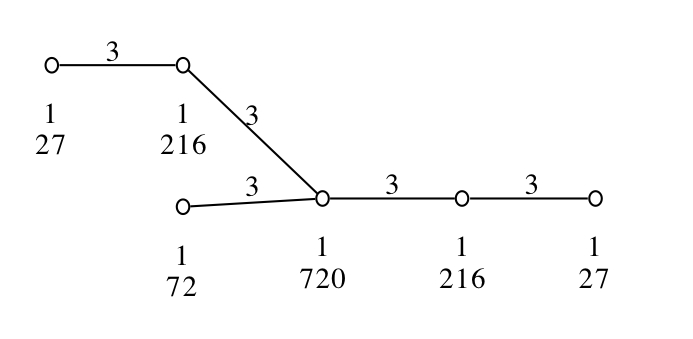
\includegraphics{./graphics/E6.jpg} 
\subsection{\textcolor{Chapter }{A rank 4 geometry for $PSL(2,11)$}}\logpage{[ 2, 5, 3 ]}
\hyperdef{L}{X85572D5782665476}{}
{


 Here we look at a particular flag-transitive geometry constructed from four
subgroups of $PSL(2,11)$, and we construct the diagram for this geometry. To view this diagram, you
need to either use a postscript viewer or a dotty viewer (such as GraphViz). 
\begin{Verbatim}[commandchars=!@|,fontsize=\small,frame=single,label=Example]
  !gapprompt@gap>| !gapinput@g := PSL(2,11);|
  Group([ (3,11,9,7,5)(4,12,10,8,6), (1,2,8)(3,7,9)(4,10,5)(6,12,11) ])
  !gapprompt@gap>| !gapinput@g1 := Group([ (1,2,3)(4,8,12)(5,10,9)(6,11,7), (1,2)(3,4)(5,12)(6,11)(7,10)(8,9) ]);|
  Group([ (1,2,3)(4,8,12)(5,10,9)(6,11,7), (1,2)(3,4)(5,12)(6,11)(7,10)(8,9) ])
  !gapprompt@gap>| !gapinput@g2 := Group([ (1,2,7)(3,9,4)(5,11,10)(6,8,12), (1,2)(3,4)(5,12)(6,11)(7,10)(8,9) ]);|
  Group([ (1,2,7)(3,9,4)(5,11,10)(6,8,12), (1,2)(3,4)(5,12)(6,11)(7,10)(8,9) ])
  !gapprompt@gap>| !gapinput@g3 := Group([ (1,2,11)(3,8,7)(4,9,5)(6,10,12), (1,2)(3,12)(4,11)(5,10)(6,9)(7,8) ]);|
  Group([ (1,2,11)(3,8,7)(4,9,5)(6,10,12), (1,2)(3,12)(4,11)(5,10)(6,9)(7,8) ])
  !gapprompt@gap>| !gapinput@g4 := Group([ (1,2,11)(3,8,7)(4,9,5)(6,10,12), (1,2)(3,10)(4,9)(5,8)(6,7)(11,12) ]);|
  Group([ (1,2,11)(3,8,7)(4,9,5)(6,10,12), (1,2)(3,10)(4,9)(5,8)(6,7)(11,12) ])
  !gapprompt@gap>| !gapinput@cg := CosetGeometry(g, [g1,g2,g3,g4]);|
  CosetGeometry( Group( [ ( 3,11, 9, 7, 5)( 4,12,10, 8, 6), 
    ( 1, 2, 8)( 3, 7, 9)( 4,10, 5)( 6,12,11) ] ) )
  !gapprompt@gap>| !gapinput@SetName(cg, "Gamma");|
  !gapprompt@gap>| !gapinput@ParabolicSubgroups(cg);|
  [ Group([ (1,2,3)(4,8,12)(5,10,9)(6,11,7), (1,2)(3,4)(5,12)(6,11)(7,10)
    (8,9) ]), Group([ (1,2,7)(3,9,4)(5,11,10)(6,8,12), (1,2)(3,4)(5,12)(6,11)
    (7,10)(8,9) ]), Group([ (1,2,11)(3,8,7)(4,9,5)(6,10,12), (1,2)(3,12)(4,11)
    (5,10)(6,9)(7,8) ]), Group([ (1,2,11)(3,8,7)(4,9,5)(6,10,12), (1,2)(3,10)
    (4,9)(5,8)(6,7)(11,12) ]) ]
  !gapprompt@gap>| !gapinput@BorelSubgroup(cg);|
  Group(())
  !gapprompt@gap>| !gapinput@AmbientGroup(cg);|
  Group([ (3,11,9,7,5)(4,12,10,8,6), (1,2,8)(3,7,9)(4,10,5)(6,12,11) ])
  !gapprompt@gap>| !gapinput@type2 := ElementsOfIncidenceStructure( cg, 2 );|
  <elements of type 2 of Gamma>
  !gapprompt@gap>| !gapinput@IsFlagTransitiveGeometry( cg );|
  true
  !gapprompt@gap>| !gapinput@DrawDiagram( DiagramOfGeometry(cg), "PSL211");|
   
\end{Verbatim}
 The output of this example uses \texttt{dotty} which is a sophisticated graph drawing program. We also provide \texttt{DrawDiagramWithNeato} to make a diagram with straight lines, using \texttt{neato}. Here is what the output looks like with the standard \texttt{DrawDiagram} command:  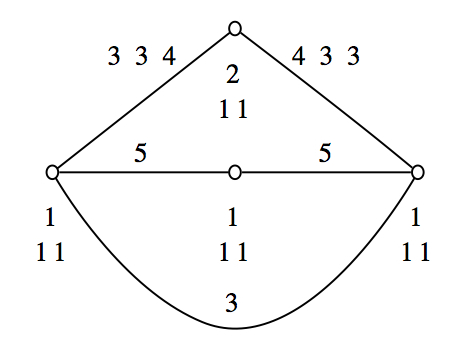
\includegraphics{./graphics/PSL211.jpg} }

 
\subsection{\textcolor{Chapter }{The Ree-Tits octagon of order $[2,4]$ as coset geometry}}\logpage{[ 2, 5, 4 ]}
\hyperdef{L}{X787388FA7DABA2D6}{}
{


 In this example we construct the Ree-Tits octagon of order $[2,4]$ as a coset geometry. From the computation of the so-called rank 2 parameters,
it can be observed already that the constructed geometry must be a generalised
octagon. Then the points and lines are computed explicitely, and together with
the incidence and the available group as a subgroup of the collineation group,
a generalised octagon is constructed.
\begin{Verbatim}[commandchars=!@|,fontsize=\small,frame=single,label=Example]
  !gapprompt@gap>| !gapinput@LoadPackage( "AtlasRep" );|
  true
  !gapprompt@gap>| !gapinput@titsgroup:=AtlasGroup("2F4(2)'");|
  <permutation group of size 17971200 with 2 generators>
  !gapprompt@gap>| !gapinput@g1:=AtlasSubgroup(titsgroup,3);|
  <permutation group of size 10240 with 2 generators>
  !gapprompt@gap>| !gapinput@g2:=AtlasSubgroup(titsgroup,5);|
  <permutation group of size 6144 with 2 generators>
  !gapprompt@gap>| !gapinput@conj:=ConjugacyClassSubgroups(titsgroup,g1);;|
  !gapprompt@gap>| !gapinput@# Now look for the conjugate of g1 with maximal intersection|
  !gapprompt@gap>| !gapinput@g1:=First(conj, sg -> Size(Intersection(sg,g2))=2048);|
  <permutation group of size 10240 with 2 generators>
  !gapprompt@gap>| !gapinput@cg:=CosetGeometry(titsgroup,[g1,g2]);;|
  !gapprompt@gap>| !gapinput@Rank2Parameters(cg);|
  [ [ 8, 8, 8 ], [ 2, 1755 ], [ 4, 2925 ] ]
  !gapprompt@gap>| !gapinput@pts := Set(ElementsOfIncidenceStructure(cg,1));;|
  !gapprompt@gap>| !gapinput@lines := Set(ElementsOfIncidenceStructure(cg,2));;|
  !gapprompt@gap>| !gapinput@gp := GeneralisedPolygonByElements(pts,lines,\*,titsgroup,OnCosetGeometryElement);|
  <generalised octagon of order [ 2, 4 ]>
  
\end{Verbatim}
 }

 }

 
\section{\textcolor{Chapter }{Elation generalised quadrangles}}\logpage{[ 2, 6, 0 ]}
\hyperdef{L}{X7BA462527B2777BC}{}
{
  In this section, we construct a classical elation generalised quadrangle from
a q-clan, and we see that the associated BLT-set is a conic. 
\subsection{\textcolor{Chapter }{The classical q-clan}}\logpage{[ 2, 6, 1 ]}
\hyperdef{L}{X7E3707857A74AB5E}{}
{


 
\begin{Verbatim}[commandchars=!@|,fontsize=\small,frame=single,label=Example]
  !gapprompt@gap>| !gapinput@f := GF(3);|
  GF(3)
  !gapprompt@gap>| !gapinput@id := IdentityMat(2, f);;|
  !gapprompt@gap>| !gapinput@clan := List( f, t -> t*id );;|
  !gapprompt@gap>| !gapinput@IsqClan( clan, f );|
  true
  !gapprompt@gap>| !gapinput@clan := qClan(clan, f);|
  <q-clan over GF(3)>
  !gapprompt@gap>| !gapinput@egq := EGQByqClan( clan );|
  #I  Computed Kantor family. Now computing EGQ...
  <EGQ of order [ 9, 3 ] and basepoint 0>
  !gapprompt@gap>| !gapinput@elations := ElationGroup( egq );|
  <matrix group of size 243 with 8 generators>
  !gapprompt@gap>| !gapinput@points := Points( egq );|
  <points of <EGQ of order [ 9, 3 ] and basepoint 0>>
  !gapprompt@gap>| !gapinput@p := Random(points);|
  <a point of class 2 of <EGQ of order [ 9, 3 ] and basepoint 0>>
  !gapprompt@gap>| !gapinput@x := Random(elations);|
  [ [ Z(3)^0, 0*Z(3), 0*Z(3), Z(3)^0 ], [ 0*Z(3), Z(3)^0, 0*Z(3), Z(3)^0 ], 
    [ 0*Z(3), 0*Z(3), Z(3)^0, Z(3)^0 ], [ 0*Z(3), 0*Z(3), 0*Z(3), Z(3)^0 ] ]
  !gapprompt@gap>| !gapinput@OnKantorFamily(p,x);|
  <a point of class 2 of <EGQ of order [ 9, 3 ] and basepoint 0>>
  !gapprompt@gap>| !gapinput@orbs := Orbits( elations, points, OnKantorFamily);;|
  !gapprompt@gap>| !gapinput@Collected(List( orbs, Size ));|
  [ [ 1, 1 ], [ 9, 4 ], [ 243, 1 ] ]
  !gapprompt@gap>| !gapinput@blt := BLTSetByqClan( clan );|
  [ <a point in Q(4, 3): -x_1*x_5-x_2*x_4+x_3^2=0>, 
    <a point in Q(4, 3): -x_1*x_5-x_2*x_4+x_3^2=0>, 
    <a point in Q(4, 3): -x_1*x_5-x_2*x_4+x_3^2=0>, 
    <a point in Q(4, 3): -x_1*x_5-x_2*x_4+x_3^2=0> ]
  !gapprompt@gap>| !gapinput@q4q := AmbientGeometry( blt[1] );|
  Q(4, 3): -x_1*x_5-x_2*x_4+x_3^2=0
  !gapprompt@gap>| !gapinput@span := Span( blt );|
  <a plane in ProjectiveSpace(4, 3)>
  !gapprompt@gap>| !gapinput@ProjectiveDimension( span ); |
  2
   
\end{Verbatim}
 }

 
\subsection{\textcolor{Chapter }{Two ways to construct a flock generalised quadrangle from a Kantor-Knuth
semifield q-clan}}\logpage{[ 2, 6, 2 ]}
\hyperdef{L}{X83357ED78789111E}{}
{
  We will construct an elation generalised quadrangle directly from the \emph{Kantor-Knuth semifield q-clan} and also via its corresponding BLT-set. The q-clan in question here are the
set of matrices $C_t$ of the form  $ \left(\begin{array}{cc} t & 0 \\ 0 & -nt^\phi \end{array}\right) $  where t runs over the elements of $GF(q)$, $q$ is odd and not prime, $n$ is a fixed nonsquare and $\phi$ is a nontrivial automorphism of $GF(q)$. 
\begin{Verbatim}[commandchars=!@|,fontsize=\small,frame=single,label=Example]
  !gapprompt@gap>| !gapinput@q := 9;|
  9
  !gapprompt@gap>| !gapinput@f := GF(q);|
  GF(3^2)
  !gapprompt@gap>| !gapinput@squares := AsList(Group(Z(q)^2));|
  [ Z(3)^0, Z(3^2)^6, Z(3), Z(3^2)^2 ]
  !gapprompt@gap>| !gapinput@n := First(GF(q), x -> not IsZero(x) and not x in squares);|
  Z(3^2)
  !gapprompt@gap>| !gapinput@sigma := FrobeniusAutomorphism( f );|
  FrobeniusAutomorphism( GF(3^2) )
  !gapprompt@gap>| !gapinput@zero := Zero(f);|
  0*Z(3)
  !gapprompt@gap>| !gapinput@qclan := List(GF(q), t -> [[t, zero], [zero,-n * t^sigma]] );|
  [ [ [ 0*Z(3), 0*Z(3) ], [ 0*Z(3), 0*Z(3) ] ], 
    [ [ Z(3^2), 0*Z(3) ], [ 0*Z(3), Z(3)^0 ] ], 
    [ [ Z(3^2)^5, 0*Z(3) ], [ 0*Z(3), Z(3) ] ], 
    [ [ Z(3)^0, 0*Z(3) ], [ 0*Z(3), Z(3^2)^5 ] ], 
    [ [ Z(3^2)^2, 0*Z(3) ], [ 0*Z(3), Z(3^2)^3 ] ], 
    [ [ Z(3^2)^3, 0*Z(3) ], [ 0*Z(3), Z(3^2)^6 ] ], 
    [ [ Z(3), 0*Z(3) ], [ 0*Z(3), Z(3^2) ] ], 
    [ [ Z(3^2)^7, 0*Z(3) ], [ 0*Z(3), Z(3^2)^2 ] ], 
    [ [ Z(3^2)^6, 0*Z(3) ], [ 0*Z(3), Z(3^2)^7 ] ] ]
  !gapprompt@gap>| !gapinput@IsqClan( qclan, f );|
  true
  !gapprompt@gap>| !gapinput@qclan := qClan(qclan , f);|
  <q-clan over GF(3^2)>
  !gapprompt@gap>| !gapinput@egq1 := EGQByqClan( qclan);  |
  #I  Computed Kantor family. Now computing EGQ...
  <EGQ of order [ 81, 9 ] and basepoint 0>
  !gapprompt@gap>| !gapinput@blt := BLTSetByqClan( qclan );|
  [ <a point in Q(4, 9): -x_1*x_5-x_2*x_4+Z(3^2)^5*x_3^2=0>, 
    <a point in Q(4, 9): -x_1*x_5-x_2*x_4+Z(3^2)^5*x_3^2=0>, 
    <a point in Q(4, 9): -x_1*x_5-x_2*x_4+Z(3^2)^5*x_3^2=0>, 
    <a point in Q(4, 9): -x_1*x_5-x_2*x_4+Z(3^2)^5*x_3^2=0>, 
    <a point in Q(4, 9): -x_1*x_5-x_2*x_4+Z(3^2)^5*x_3^2=0>, 
    <a point in Q(4, 9): -x_1*x_5-x_2*x_4+Z(3^2)^5*x_3^2=0>, 
    <a point in Q(4, 9): -x_1*x_5-x_2*x_4+Z(3^2)^5*x_3^2=0>, 
    <a point in Q(4, 9): -x_1*x_5-x_2*x_4+Z(3^2)^5*x_3^2=0>, 
    <a point in Q(4, 9): -x_1*x_5-x_2*x_4+Z(3^2)^5*x_3^2=0>, 
    <a point in Q(4, 9): -x_1*x_5-x_2*x_4+Z(3^2)^5*x_3^2=0> ]
  !gapprompt@gap>| !gapinput@egq2 := EGQByBLTSet( blt );|
  #I  Now embedding dual BLT-set into W(5,q)...
  #I  Computing elation group...
  <EGQ of order [ 81, 9 ] and basepoint in W(5, 9 ) >
   
\end{Verbatim}
 }

 }

 
\section{\textcolor{Chapter }{Algebraic varieties}}\logpage{[ 2, 7, 0 ]}
\hyperdef{L}{X87EC44BF7F24486E}{}
{
  
\subsection{\textcolor{Chapter }{A projective variety}}\logpage{[ 2, 7, 1 ]}
\hyperdef{L}{X7ABCF9637B60FF37}{}
{


 In this example we demonstrate the construction of projective varieties. 
\begin{Verbatim}[commandchars=!@|,fontsize=\small,frame=single,label=Example]
  !gapprompt@gap>| !gapinput@pg1 := PG(1, 7);|
  ProjectiveSpace(1, 7)
  !gapprompt@gap>| !gapinput@pg3 := PG(3, 7);|
  ProjectiveSpace(3, 7)
  !gapprompt@gap>| !gapinput@points := Points(pg1);|
  <points of ProjectiveSpace(1, 7)>
  !gapprompt@gap>| !gapinput@coords := List(points, Coordinates);|
  [ [ Z(7)^0, 0*Z(7) ], [ Z(7)^0, Z(7)^0 ], [ Z(7)^0, Z(7) ], 
    [ Z(7)^0, Z(7)^2 ], [ Z(7)^0, Z(7)^3 ], [ Z(7)^0, Z(7)^4 ], 
    [ Z(7)^0, Z(7)^5 ], [ 0*Z(7), Z(7)^0 ] ]
  !gapprompt@gap>| !gapinput@curve := List(coords, t -> VectorSpaceToElement(pg3, [ t[1]^3, t[1]^2 * t[2], t[1] * t[2]^2, t[2]^3  ] ));;|
  !gapprompt@gap>| !gapinput@pgl := ProjectivityGroup( pg3 );|
  The FinInG projectivity group PGL(4,7)
  !gapprompt@gap>| !gapinput@stabcurve := FiningSetwiseStabiliser( pgl, curve );|
  #I  Computing adjusted stabilizer chain...
  <projective collineation group with 6 generators>
  !gapprompt@gap>| !gapinput@StructureDescription( stabcurve );|
  "PSL(3,2) : C2"
  !gapprompt@gap>| !gapinput@Span( curve );|
  ProjectiveSpace(3, 7)
  !gapprompt@gap>| !gapinput@pg3lines := Lines( pg3 );|
  <lines of ProjectiveSpace(3, 7)>
  !gapprompt@gap>| !gapinput@orbits := FiningOrbits(stabcurve, pg3lines);|
  2%..3%..9%..15%..16%..21%..22%..28%..34%..40%..46%..52%..64%..75%..81%..84%..88%..94%..95%..99%..100%..[ <closed orbit, 8 points>, <closed orbit, 56 points>, 
    <closed orbit, 28 points>, <closed orbit, 168 points>, 
    <closed orbit, 168 points>, <closed orbit, 28 points>, 
    <closed orbit, 168 points>, <closed orbit, 28 points>, 
    <closed orbit, 168 points>, <closed orbit, 168 points>, 
    <closed orbit, 168 points>, <closed orbit, 168 points>, 
    <closed orbit, 168 points>, <closed orbit, 336 points>, 
    <closed orbit, 336 points>, <closed orbit, 168 points>, 
    <closed orbit, 84 points>, <closed orbit, 112 points>, 
    <closed orbit, 168 points>, <closed orbit, 21 points>, 
    <closed orbit, 112 points>, <closed orbit, 21 points> ]
  !gapprompt@gap>| !gapinput@List(orbits, Size);|
  [ 8, 56, 28, 168, 168, 28, 168, 28, 168, 168, 168, 168, 168, 336, 336, 168, 
    84, 112, 168, 21, 112, 21 ]
  !gapprompt@gap>| !gapinput@pg3points := Points( pg3 );|
  <points of ProjectiveSpace(3, 7)>
  !gapprompt@gap>| !gapinput@orbits := FiningOrbits(stabcurve, pg3points);|
  2%..16%..30%..72%..100%..[ <closed orbit, 8 points>, <closed orbit, 56 points>, 
    <closed orbit, 56 points>, <closed orbit, 168 points>, 
    <closed orbit, 112 points> ]
  !gapprompt@gap>| !gapinput@List(orbits, Size);|
  [ 8, 56, 56, 168, 112 ]
  !gapprompt@gap>| !gapinput@reps := List(orbits, Representative);|
  [ <a point in ProjectiveSpace(3, 7)>, <a point in ProjectiveSpace(3, 7)>, 
    <a point in ProjectiveSpace(3, 7)>, <a point in ProjectiveSpace(3, 7)>, 
    <a point in ProjectiveSpace(3, 7)> ]
  !gapprompt@gap>| !gapinput@x := reps[2];|
  <a point in ProjectiveSpace(3, 7)>
  !gapprompt@gap>| !gapinput@proj := NaturalProjectionBySubspace(pg3, x);|
  <geometry morphism from <All elements of ProjectiveSpace(3, 
  7)> to <All elements of ProjectiveSpace(2, 7)>>
  !gapprompt@gap>| !gapinput@curveminusx := Difference(curve, [x]);|
  [ <a point in ProjectiveSpace(3, 7)>, <a point in ProjectiveSpace(3, 7)>, 
    <a point in ProjectiveSpace(3, 7)>, <a point in ProjectiveSpace(3, 7)>, 
    <a point in ProjectiveSpace(3, 7)>, <a point in ProjectiveSpace(3, 7)>, 
    <a point in ProjectiveSpace(3, 7)>, <a point in ProjectiveSpace(3, 7)> ]
  !gapprompt@gap>| !gapinput@cuspidal := ImagesSet(proj, List(curveminusx, t -> Span(x, t)));|
  [ <a point in ProjectiveSpace(2, 7)>, <a point in ProjectiveSpace(2, 7)>, 
    <a point in ProjectiveSpace(2, 7)>, <a point in ProjectiveSpace(2, 7)>, 
    <a point in ProjectiveSpace(2, 7)>, <a point in ProjectiveSpace(2, 7)>, 
    <a point in ProjectiveSpace(2, 7)>, <a point in ProjectiveSpace(2, 7)> ]
  !gapprompt@gap>| !gapinput@coords := List(cuspidal, Coordinates);|
  [ [ Z(7)^0, 0*Z(7), 0*Z(7) ], [ 0*Z(7), 0*Z(7), Z(7)^0 ], 
    [ Z(7)^0, Z(7)^0, Z(7)^0 ], [ Z(7)^0, Z(7)^2, Z(7)^0 ], 
    [ Z(7)^0, Z(7)^4, Z(7)^0 ], [ Z(7)^0, Z(7)^0, Z(7)^3 ], 
    [ Z(7)^0, Z(7)^2, Z(7)^3 ], [ Z(7)^0, Z(7)^4, Z(7)^3 ] ]
  !gapprompt@gap>| !gapinput@r := PolynomialRing(GF(7), 3);|
  GF(7)[x_1,x_2,x_3]
  !gapprompt@gap>| !gapinput@indets := IndeterminatesOfPolynomialRing(r);|
  [ x_1, x_2, x_3 ]
  !gapprompt@gap>| !gapinput@shapes := Filtered(Tuples([0,1,2,3], 3), t -> Sum(t) = 3);|
  [ [ 0, 0, 3 ], [ 0, 1, 2 ], [ 0, 2, 1 ], [ 0, 3, 0 ], [ 1, 0, 2 ], 
    [ 1, 1, 1 ], [ 1, 2, 0 ], [ 2, 0, 1 ], [ 2, 1, 0 ], [ 3, 0, 0 ] ]
  !gapprompt@gap>| !gapinput@mat := List(coords, t -> List(shapes, u -> Product([1,2,3], i -> t[i]^u[i])));|
  [ [ 0*Z(7), 0*Z(7), 0*Z(7), 0*Z(7), 0*Z(7), 0*Z(7), 0*Z(7), 0*Z(7), 0*Z(7), 
        Z(7)^0 ], 
    [ Z(7)^0, 0*Z(7), 0*Z(7), 0*Z(7), 0*Z(7), 0*Z(7), 0*Z(7), 0*Z(7), 0*Z(7), 
        0*Z(7) ], 
    [ Z(7)^0, Z(7)^0, Z(7)^0, Z(7)^0, Z(7)^0, Z(7)^0, Z(7)^0, Z(7)^0, Z(7)^0, 
        Z(7)^0 ], 
    [ Z(7)^0, Z(7)^2, Z(7)^4, Z(7)^0, Z(7)^0, Z(7)^2, Z(7)^4, Z(7)^0, Z(7)^2, 
        Z(7)^0 ], 
    [ Z(7)^0, Z(7)^4, Z(7)^2, Z(7)^0, Z(7)^0, Z(7)^4, Z(7)^2, Z(7)^0, Z(7)^4, 
        Z(7)^0 ], 
    [ Z(7)^3, Z(7)^0, Z(7)^3, Z(7)^0, Z(7)^0, Z(7)^3, Z(7)^0, Z(7)^3, Z(7)^0, 
        Z(7)^0 ], 
    [ Z(7)^3, Z(7)^2, Z(7), Z(7)^0, Z(7)^0, Z(7)^5, Z(7)^4, Z(7)^3, Z(7)^2, 
        Z(7)^0 ], 
    [ Z(7)^3, Z(7)^4, Z(7)^5, Z(7)^0, Z(7)^0, Z(7), Z(7)^2, Z(7)^3, Z(7)^4, 
        Z(7)^0 ] ]
  !gapprompt@gap>| !gapinput@mat2 := ShallowCopy(mat);|
  [ [ 0*Z(7), 0*Z(7), 0*Z(7), 0*Z(7), 0*Z(7), 0*Z(7), 0*Z(7), 0*Z(7), 0*Z(7), 
        Z(7)^0 ], 
    [ Z(7)^0, 0*Z(7), 0*Z(7), 0*Z(7), 0*Z(7), 0*Z(7), 0*Z(7), 0*Z(7), 0*Z(7), 
        0*Z(7) ], 
    [ Z(7)^0, Z(7)^0, Z(7)^0, Z(7)^0, Z(7)^0, Z(7)^0, Z(7)^0, Z(7)^0, Z(7)^0, 
        Z(7)^0 ], 
    [ Z(7)^0, Z(7)^2, Z(7)^4, Z(7)^0, Z(7)^0, Z(7)^2, Z(7)^4, Z(7)^0, Z(7)^2, 
        Z(7)^0 ], 
    [ Z(7)^0, Z(7)^4, Z(7)^2, Z(7)^0, Z(7)^0, Z(7)^4, Z(7)^2, Z(7)^0, Z(7)^4, 
        Z(7)^0 ], 
    [ Z(7)^3, Z(7)^0, Z(7)^3, Z(7)^0, Z(7)^0, Z(7)^3, Z(7)^0, Z(7)^3, Z(7)^0, 
        Z(7)^0 ], 
    [ Z(7)^3, Z(7)^2, Z(7), Z(7)^0, Z(7)^0, Z(7)^5, Z(7)^4, Z(7)^3, Z(7)^2, 
        Z(7)^0 ], 
    [ Z(7)^3, Z(7)^4, Z(7)^5, Z(7)^0, Z(7)^0, Z(7), Z(7)^2, Z(7)^3, Z(7)^4, 
        Z(7)^0 ] ]
  !gapprompt@gap>| !gapinput@sol := NullspaceMat(TransposedMat(mat2))[1];|
  [ 0*Z(7), 0*Z(7), 0*Z(7), Z(7)^3, Z(7)^0, 0*Z(7), 0*Z(7), 0*Z(7), 0*Z(7),
     0*Z(7) ]
  !gapprompt@gap>| !gapinput@terms := List(shapes, u -> Product([1,2,3], i -> indets[i]^u[i]));|
  [ x_3^3, x_2*x_3^2, x_2^2*x_3, x_2^3, x_1*x_3^2, x_1*x_2*x_3, x_1*x_2^2, 
    x_1^2*x_3, x_1^2*x_2, x_1^3 ]
  !gapprompt@gap>| !gapinput@poly := terms * sol;|
  x_1*x_3^2-x_2^3
  !gapprompt@gap>| !gapinput@pg2 := AmbientGeometry(Range(proj));|
  ProjectiveSpace(2, 7)
  !gapprompt@gap>| !gapinput@variety := ProjectiveVariety(pg2, [poly]);|
  Projective Variety in ProjectiveSpace(2, 7)
  !gapprompt@gap>| !gapinput@points := Points(variety);|
  <points of Projective Variety in ProjectiveSpace(2, 7)>
  !gapprompt@gap>| !gapinput@Size(points);|
  8
   
\end{Verbatim}
 }

 }

 }

  
\chapter{\textcolor{Chapter }{Incidence Geometry}}\label{incidencegeometry}
\logpage{[ 3, 0, 0 ]}
\hyperdef{L}{X838ACF8A7F100A2B}{}
{
  We follow \cite{BC2013} for the definitions of incidence structure and incidence geometry. An \emph{incidence structure} consists of a set of elements, a symmetric relation on the elements and a type
function from the set of elements to an index set (i.e., every element has a
``type''). It satisfies the following axiom: \emph{(i) no two elements of the same type are incident.} An incidence structure without type function is in fact a multipartite graph
where the adjacency is the incidence (so with a loop on each vertex). The term
geometry, or incidence geometry, is interpreted broadly in this package.
Particularly, an \emph{incidence geometry} is an incidence structure satisfying the following axiom: \emph{(ii) every maximal flag contains an element of each type}. In graph terminology, this means that every maximal clique contains an
element of each type. Thus, a projective 5-space is an incidence geometry with
five types of elements: points, lines, planes, solids, and hyperplanes. A
finite classical polar space of rank 3 is an incidence geometry with three
types of elements: points, lines, and planes. Depending on the viewpoint, the
Grassmann variety of the lines of a projective 4-space, is an incidence
structure that is not an incidence geometry.

 \textsf{FinInG} concerns itself primarily with the most commonly studied incidence geometries
of rank at least 2: projective spaces, polar spaces, and affine spaces.
Throughout, no matter the geometry, we have made the convention that an
element of type 1 is a ``point'', an element of type 2 is a ``line'', and so
forth. The examples we use in this section use projective spaces, which have
not yet been introduced to the reader in this manual. For further information
on projective spaces, see Chapter \ref{projective_spaces}.

 In this chapter we describe functionality that is \textsc{declared} for incidence structures, which does not imply that operations described here
will work for arbitrary user-constructed incidence structures. Its aim is
furthermore to allow the user to become familiar with the general philosophy
of the package, using examples that are self-explanatory. Not all details of
the commands used in the examples will be explained in this chapter, therefore
we refer to the relevant chapter for the commands. These can easily be found
using the index. 
\section{\textcolor{Chapter }{Incidence structures}}\logpage{[ 3, 1, 0 ]}
\hyperdef{L}{X7FB175337C4F8B76}{}
{
  Incidence structures can be more general than incidence geometries, e.g., if
they do not satisfy axiom (ii) mentioned above. We allow the construction of
such objects. This explains one of the top level categories in \textsf{FinInG}. 

\subsection{\textcolor{Chapter }{IsIncidenceStructure}}
\logpage{[ 3, 1, 1 ]}\nobreak
\hyperdef{L}{X81F7D8FA82A55561}{}
{\noindent\textcolor{FuncColor}{$\triangleright$\ \ \texttt{IsIncidenceStructure\index{IsIncidenceStructure@\texttt{IsIncidenceStructure}}
\label{IsIncidenceStructure}
}\hfill{\scriptsize (Category)}}\\


 Top level category for all objects representing an incidence structure. }

 

\subsection{\textcolor{Chapter }{IsIncidenceGeometry}}
\logpage{[ 3, 1, 2 ]}\nobreak
\hyperdef{L}{X78C74BE87E050E84}{}
{\noindent\textcolor{FuncColor}{$\triangleright$\ \ \texttt{IsIncidenceGeometry\index{IsIncidenceGeometry@\texttt{IsIncidenceGeometry}}
\label{IsIncidenceGeometry}
}\hfill{\scriptsize (Category)}}\\


 Category for all objects representing an incidence geometry. All particular
geometries implemented in \textsf{FinInG} are incidence geometries. }

 

\subsection{\textcolor{Chapter }{IncidenceStructure}}
\logpage{[ 3, 1, 3 ]}\nobreak
\label{oper:incidencestructure}
\hyperdef{L}{X7C3258887C8DF5C1}{}
{\noindent\textcolor{FuncColor}{$\triangleright$\ \ \texttt{IncidenceStructure({\mdseries\slshape eles, inc{\textunderscore}rel, type, typeset})\index{IncidenceStructure@\texttt{IncidenceStructure}}
\label{IncidenceStructure}
}\hfill{\scriptsize (operation)}}\\
\textbf{\indent Returns:\ }
an incidence structure



 \mbox{\texttt{\mdseries\slshape eles}} is a set containing the elements of the incidence structure. \mbox{\texttt{\mdseries\slshape inc{\textunderscore}rel}} must be a function that determines whether two objects in the set \mbox{\texttt{\mdseries\slshape eles}} are incident. \mbox{\texttt{\mdseries\slshape type}} is a function mapping any element to its type, which is a unique element in
the set \mbox{\texttt{\mdseries\slshape typeset}}.

 In the following example we define an incidence structure that is not an
incidence geometry. The example used is the incidence structure with elements
the subspaces contained in the line Grassmannian of PG(4,2). This example is
not meant to create this incidence structure in an efficient way, but just to
demonstrate the general philosophy. 
\begin{Verbatim}[commandchars=!@|,fontsize=\small,frame=single,label=Example]
  !gapprompt@gap>| !gapinput@pg := PG(4,2);|
  ProjectiveSpace(4, 2)
  !gapprompt@gap>| !gapinput@pg2 := PG(9,2);|
  ProjectiveSpace(9, 2)
  !gapprompt@gap>| !gapinput@points := List(Lines(pg),x->VectorSpaceToElement(pg2,GrassmannCoordinates(x)));;|
  !gapprompt@gap>| !gapinput@flags := Concatenation(List(Points(pg),x->List(Planes(x),y->FlagOfIncidenceStructure(pg,[x,y]))));;|
  !gapprompt@gap>| !gapinput@prelines := List(flags,flag->ShadowOfFlag(pg,flag,2));;|
  !gapprompt@gap>| !gapinput@lines := List(prelines,x->VectorSpaceToElement(pg2,List(x,y->GrassmannCoordinates(y))));;|
  !gapprompt@gap>| !gapinput@flags2 := Concatenation(List(Points(pg),x->List(Solids(x),y->FlagOfIncidenceStructure(pg,[x,y]))));;|
  !gapprompt@gap>| !gapinput@preplanes := List(flags2,flag->ShadowOfFlag(pg,flag,2));;|
  !gapprompt@gap>| !gapinput@planes := List(preplanes,x->VectorSpaceToElement(pg2,List(x,y->GrassmannCoordinates(y))));;|
  !gapprompt@gap>| !gapinput@maximals1 := List(Planes(pg),x->VectorSpaceToElement(pg2,List(Lines(x),y->GrassmannCoordinates(y))));;|
  !gapprompt@gap>| !gapinput@maximals2 := List(Points(pg),x->VectorSpaceToElement(pg2,List(Lines(x),y->GrassmannCoordinates(y))));;|
  !gapprompt@gap>| !gapinput@elements := Union(points,lines,planes,maximals1,maximals2);;|
  !gapprompt@gap>| !gapinput@Length(elements);|
  1891
  !gapprompt@gap>| !gapinput@type := x -> ProjectiveDimension(x)+1;|
  function( x ) ... end
  !gapprompt@gap>| !gapinput@inc_rel := \*;|
  <Operation "*">
  !gapprompt@gap>| !gapinput@inc := IncidenceStructure(elements,inc_rel,type,[1,2,3,4]);|
  Incidence structure of rank 4
  !gapprompt@gap>| !gapinput@Rank(inc);|
  4
  
  
\end{Verbatim}
 }

 Lie Geometries, i.e., geometries with a projective space as ambient space,
affine spaces and generalised polygons have their own category, which is a
subcategory of \texttt{IsIncidenceGeometry}. 
\subsection{\textcolor{Chapter }{Main categories in \texttt{IsIncidenceGeometry}}}\logpage{[ 3, 1, 4 ]}
\hyperdef{L}{X7EB285F379512585}{}
{
\noindent\textcolor{FuncColor}{$\triangleright$\ \ \texttt{IsLieGeometry\index{IsLieGeometry@\texttt{IsLieGeometry}}
\label{IsLieGeometry}
}\hfill{\scriptsize (Category)}}\\
\noindent\textcolor{FuncColor}{$\triangleright$\ \ \texttt{IsAffineSpace\index{IsAffineSpace@\texttt{IsAffineSpace}}
\label{IsAffineSpace}
}\hfill{\scriptsize (Category)}}\\
\noindent\textcolor{FuncColor}{$\triangleright$\ \ \texttt{IsGeneralisedPolygon\index{IsGeneralisedPolygon@\texttt{IsGeneralisedPolygon}}
\label{IsGeneralisedPolygon}
}\hfill{\scriptsize (Category)}}\\
\noindent\textcolor{FuncColor}{$\triangleright$\ \ \texttt{IsCosetGeometry\index{IsCosetGeometry@\texttt{IsCosetGeometry}}
\label{IsCosetGeometry}
}\hfill{\scriptsize (Category)}}\\


 Within each category, several subcategories are declared. Subcategories of \texttt{IsLieGeometry} are discussed in Section \ref{liegeometries1} and subcategories of \texttt{IsGeneralisedPolygon} are discussed in Chapter \ref{gpolygons} }

 
\subsection{\textcolor{Chapter }{Examples of categories of incidence geometries}}\logpage{[ 3, 1, 5 ]}
\hyperdef{L}{X87FFB1648575FFF2}{}
{


 
\begin{Verbatim}[commandchars=!@|,fontsize=\small,frame=single,label=Example]
  !gapprompt@gap>| !gapinput@CategoriesOfObject(ProjectiveSpace(5,7));|
  [ "IsIncidenceStructure", "IsIncidenceGeometry", "IsLieGeometry", 
    "IsProjectiveSpace" ]
  !gapprompt@gap>| !gapinput@CategoriesOfObject(HermitianPolarSpace(5,9));|
  [ "IsIncidenceStructure", "IsIncidenceGeometry", "IsLieGeometry", 
    "IsClassicalPolarSpace", "IsAlgebraicVariety", "IsProjectiveVariety", 
    "IsHermitianVariety" ]
  !gapprompt@gap>| !gapinput@CategoriesOfObject(AffineSpace(3,3));|
  [ "IsIncidenceStructure", "IsIncidenceGeometry", "IsAffineSpace" ]
  !gapprompt@gap>| !gapinput@CategoriesOfObject(SymplecticSpace(3,11));|
  [ "IsIncidenceStructure", "IsIncidenceGeometry", "IsLieGeometry", 
    "IsClassicalPolarSpace", "IsGeneralisedPolygon", "IsGeneralisedQuadrangle", 
    "IsClassicalGQ" ]
  !gapprompt@gap>| !gapinput@CategoriesOfObject(SplitCayleyHexagon(9));|
  [ "IsIncidenceStructure", "IsIncidenceGeometry", "IsLieGeometry", 
    "IsGeneralisedPolygon", "IsGeneralisedHexagon", 
    "IsClassicalGeneralisedHexagon" ]
  !gapprompt@gap>| !gapinput@CategoriesOfObject(ParabolicQuadric(4,16));|
  [ "IsIncidenceStructure", "IsIncidenceGeometry", "IsLieGeometry", 
    "IsClassicalPolarSpace", "IsGeneralisedPolygon", "IsGeneralisedQuadrangle", 
    "IsClassicalGQ", "IsAlgebraicVariety", "IsProjectiveVariety" ]
   
\end{Verbatim}
 }

 

\subsection{\textcolor{Chapter }{TypesOfElementsOfIncidenceStructure}}
\logpage{[ 3, 1, 6 ]}\nobreak
\hyperdef{L}{X7E574AB27DA97063}{}
{\noindent\textcolor{FuncColor}{$\triangleright$\ \ \texttt{TypesOfElementsOfIncidenceStructure({\mdseries\slshape inc})\index{TypesOfElementsOfIncidenceStructure@\texttt{TypesOfElementsOfIncidenceStructure}}
\label{TypesOfElementsOfIncidenceStructure}
}\hfill{\scriptsize (attribute)}}\\
\noindent\textcolor{FuncColor}{$\triangleright$\ \ \texttt{TypesOfElementsOfIncidenceStructurePlural({\mdseries\slshape inc})\index{TypesOfElementsOfIncidenceStructurePlural@\texttt{Types}\-\texttt{Of}\-\texttt{Elements}\-\texttt{Of}\-\texttt{Incidence}\-\texttt{Structure}\-\texttt{Plural}}
\label{TypesOfElementsOfIncidenceStructurePlural}
}\hfill{\scriptsize (attribute)}}\\
\textbf{\indent Returns:\ }
a list of strings or integers



 Both attributes are declared for objects in the category \texttt{IsIncidenceStructure}. Any incidence structure has a set of types, which is usually just the list ${1..n}$. If specific names are given to each type, like points, lines, etc., this
attribute returns the names for the particular incidence structure \mbox{\texttt{\mdseries\slshape inc}}. The second variant returns the list of plurals of these names. For genericly
constructed incidence structures, the names of the Elements are also generic:
elements of type 1, elements of type 2, etc. 
\begin{Verbatim}[commandchars=!@|,fontsize=\small,frame=single,label=Example]
  !gapprompt@gap>| !gapinput@TypesOfElementsOfIncidenceStructure(ProjectiveSpace(5,4));|
  [ "point", "line", "plane", "solid", "proj. 4-space" ]
  !gapprompt@gap>| !gapinput@TypesOfElementsOfIncidenceStructurePlural(AffineSpace(7,4));|
  [ "points", "lines", "planes", "solids", "affine. subspaces of dim. 4", 
    "affine. subspaces of dim. 5", "affine. subspaces of dim. 6" ]
   
\end{Verbatim}
 }

 

\subsection{\textcolor{Chapter }{Rank}}
\logpage{[ 3, 1, 7 ]}\nobreak
\hyperdef{L}{X827146F37E2AA841}{}
{\noindent\textcolor{FuncColor}{$\triangleright$\ \ \texttt{Rank({\mdseries\slshape inc})\index{Rank@\texttt{Rank}}
\label{Rank}
}\hfill{\scriptsize (operation)}}\\
\noindent\textcolor{FuncColor}{$\triangleright$\ \ \texttt{RankAttr({\mdseries\slshape inc})\index{RankAttr@\texttt{RankAttr}}
\label{RankAttr}
}\hfill{\scriptsize (attribute)}}\\
\textbf{\indent Returns:\ }
rank of \mbox{\texttt{\mdseries\slshape inc}}, an object which must belong to the category \texttt{IsIncidenceStructure}



 The operation \texttt{Rank} returns the rank of the incidence structure \texttt{inc}. The highest level method for \texttt{Rank}, applicable to objects in \texttt{IsIncidenceStructure} simply refers to the attribute \texttt{RankAttr}. In \textsf{FinInG}, the rank of an incidence structure is determined upon creation, when also \texttt{RankAttr} is set. 
\begin{Verbatim}[commandchars=!@|,fontsize=\small,frame=single,label=Example]
  !gapprompt@gap>| !gapinput@Rank(ProjectiveSpace(5,5));|
  5
  !gapprompt@gap>| !gapinput@Rank(AffineSpace(3,5));|
  3
  !gapprompt@gap>| !gapinput@Rank(SymplecticSpace(5,5));|
  3
   
\end{Verbatim}
 }

 

\subsection{\textcolor{Chapter }{IncidenceGraph}}
\logpage{[ 3, 1, 8 ]}\nobreak
\hyperdef{L}{X815BE6D57D623452}{}
{\noindent\textcolor{FuncColor}{$\triangleright$\ \ \texttt{IncidenceGraph({\mdseries\slshape inc})\index{IncidenceGraph@\texttt{IncidenceGraph}}
\label{IncidenceGraph}
}\hfill{\scriptsize (attribute)}}\\
\textbf{\indent Returns:\ }
a graph



 The vertices are the elements of \mbox{\texttt{\mdseries\slshape inc}}, adjacency between different vertices is equal to incidence, and there are of
course no loops. For generic incidence structures, i.e. constructed through \texttt{IncidenceStructure}, there is no efficient method installed, so this operation can be time
consuming.

 If \mbox{\texttt{\mdseries\slshape inc}} is a generic incidence structure, i.e. created using \texttt{IncidenceStructure}, the vertex names of the graph are integers. It is not by default possible to
use the elements of \mbox{\texttt{\mdseries\slshape inc}} as vertex names, since it is not known in the generic case whether the
elements of different type of \mbox{\texttt{\mdseries\slshape inc}} can be ordered. For particular incidence geometries, e.g. projective spaces,
etc., the vertex names will be the elements, which will be demonstrated
through examples in the appropriate chapters.

 In the example we consider the so-called doubling of the smallest generalised
quadrangle: the points of the incidence structure are the points and the lines
of the GQ, the lines of the incidence structure are all the point-line flags
of the GQ. The incidence is the natural one. It is then checked that diameter
and girth of the incidence graph are 8 and 16 respectively, which makes that
the incidence structure is a generalised octagon. 
\begin{Verbatim}[commandchars=!@|,fontsize=\small,frame=single,label=Example]
  !gapprompt@gap>| !gapinput@ps := SymplecticSpace(3,2);|
  W(3, 2)
  !gapprompt@gap>| !gapinput@pts := List(Points(ps));;|
  !gapprompt@gap>| !gapinput@lines := List(Lines(ps));;|
  !gapprompt@gap>| !gapinput@flags := Union(List(pts,x->List(Lines(x),y->FlagOfIncidenceStructure(ps,[x,y]))));;|
  !gapprompt@gap>| !gapinput@inc := function(x,y)|
  !gapprompt@>| !gapinput@if x = y then|
  !gapprompt@>| !gapinput@    return true;|
  !gapprompt@>| !gapinput@elif IsFlagOfIncidenceStructure(x) and IsElementOfIncidenceStructure(y) then|
  !gapprompt@>| !gapinput@    return IsIncident(x,y);|
  !gapprompt@>| !gapinput@elif IsElementOfIncidenceStructure(x) and IsElementOfIncidenceStructure(y) then|
  !gapprompt@>| !gapinput@    return false;|
  !gapprompt@>| !gapinput@elif IsFlagOfIncidenceStructure(x) and IsFlagOfIncidenceStructure(y) then   |
  !gapprompt@>| !gapinput@    return false;|
  !gapprompt@>| !gapinput@else |
  !gapprompt@>| !gapinput@    return inc(y,x);|
  !gapprompt@>| !gapinput@fi;|
  !gapprompt@>| !gapinput@end;|
  function( x, y ) ... end
  !gapprompt@gap>| !gapinput@type := function(x)|
  !gapprompt@>| !gapinput@if IsList(Type(x)) then|
  !gapprompt@>| !gapinput@    return 2;|
  !gapprompt@>| !gapinput@else|
  !gapprompt@>| !gapinput@    return 1;|
  !gapprompt@>| !gapinput@fi;|
  !gapprompt@>| !gapinput@end;|
  function( x ) ... end
  !gapprompt@gap>| !gapinput@els := Union(pts,lines,flags);;|
  !gapprompt@gap>| !gapinput@struc := IncidenceStructure(els,inc,type,[1,2]);|
  Incidence structure of rank 2
  !gapprompt@gap>| !gapinput@gamma := IncidenceGraph(struc);|
  rec( adjacencies := [ [ 31, 32, 33 ], [ 34, 35, 36 ], [ 37, 38, 39 ], 
        [ 40, 41, 42 ], [ 43, 44, 45 ], [ 46, 47, 48 ], [ 49, 50, 51 ], 
        [ 52, 53, 54 ], [ 55, 56, 57 ], [ 58, 59, 60 ], [ 61, 62, 63 ], 
        [ 64, 65, 66 ], [ 67, 68, 69 ], [ 70, 71, 72 ], [ 73, 74, 75 ], 
        [ 31, 40, 43 ], [ 32, 52, 55 ], [ 33, 64, 67 ], [ 34, 41, 46 ], 
        [ 35, 53, 58 ], [ 36, 65, 70 ], [ 37, 42, 49 ], [ 38, 54, 61 ], 
        [ 39, 66, 73 ], [ 44, 59, 74 ], [ 45, 62, 71 ], [ 47, 56, 75 ], 
        [ 50, 57, 72 ], [ 48, 63, 68 ], [ 51, 60, 69 ], [ 1, 16 ], [ 1, 17 ], 
        [ 1, 18 ], [ 2, 19 ], [ 2, 20 ], [ 2, 21 ], [ 3, 22 ], [ 3, 23 ], 
        [ 3, 24 ], [ 4, 16 ], [ 4, 19 ], [ 4, 22 ], [ 5, 16 ], [ 5, 25 ], 
        [ 5, 26 ], [ 6, 19 ], [ 6, 27 ], [ 6, 29 ], [ 7, 22 ], [ 7, 28 ], 
        [ 7, 30 ], [ 8, 17 ], [ 8, 20 ], [ 8, 23 ], [ 9, 17 ], [ 9, 27 ], 
        [ 9, 28 ], [ 10, 20 ], [ 10, 25 ], [ 10, 30 ], [ 11, 23 ], [ 11, 26 ], 
        [ 11, 29 ], [ 12, 18 ], [ 12, 21 ], [ 12, 24 ], [ 13, 18 ], [ 13, 29 ], 
        [ 13, 30 ], [ 14, 21 ], [ 14, 26 ], [ 14, 28 ], [ 15, 24 ], [ 15, 25 ], 
        [ 15, 27 ] ], group := Group(()), isGraph := true, names := [ 1 .. 75 ],
    order := 75, 
    representatives := [ 1, 2, 3, 4, 5, 6, 7, 8, 9, 10, 11, 12, 13, 14, 15, 16, 
        17, 18, 19, 20, 21, 22, 23, 24, 25, 26, 27, 28, 29, 30, 31, 32, 33, 34, 
        35, 36, 37, 38, 39, 40, 41, 42, 43, 44, 45, 46, 47, 48, 49, 50, 51, 52, 
        53, 54, 55, 56, 57, 58, 59, 60, 61, 62, 63, 64, 65, 66, 67, 68, 69, 70, 
        71, 72, 73, 74, 75 ], 
    schreierVector := [ -1, -2, -3, -4, -5, -6, -7, -8, -9, -10, -11, -12, -13, 
        -14, -15, -16, -17, -18, -19, -20, -21, -22, -23, -24, -25, -26, -27, 
        -28, -29, -30, -31, -32, -33, -34, -35, -36, -37, -38, -39, -40, -41, 
        -42, -43, -44, -45, -46, -47, -48, -49, -50, -51, -52, -53, -54, -55, 
        -56, -57, -58, -59, -60, -61, -62, -63, -64, -65, -66, -67, -68, -69, 
        -70, -71, -72, -73, -74, -75 ] )
  !gapprompt@gap>| !gapinput@Diameter(gamma);|
  8
  !gapprompt@gap>| !gapinput@Girth(gamma);|
  16
  
\end{Verbatim}
 }

 }

 
\section{\textcolor{Chapter }{Elements of incidence structures}}\logpage{[ 3, 2, 0 ]}
\hyperdef{L}{X7BBDB0AE7E29F3FB}{}
{
  
\subsection{\textcolor{Chapter }{Main categories for individual elements of incidence structures}}\logpage{[ 3, 2, 1 ]}
\hyperdef{L}{X827CD3C881DC8364}{}
{
\noindent\textcolor{FuncColor}{$\triangleright$\ \ \texttt{IsElementOfIncidenceStructure\index{IsElementOfIncidenceStructure@\texttt{IsElementOfIncidenceStructure}}
\label{IsElementOfIncidenceStructure}
}\hfill{\scriptsize (Category)}}\\
\noindent\textcolor{FuncColor}{$\triangleright$\ \ \texttt{IsElementOfIncidenceGeometry\index{IsElementOfIncidenceGeometry@\texttt{IsElementOfIncidenceGeometry}}
\label{IsElementOfIncidenceGeometry}
}\hfill{\scriptsize (Category)}}\\
\noindent\textcolor{FuncColor}{$\triangleright$\ \ \texttt{IsElementOfLieGeometry\index{IsElementOfLieGeometry@\texttt{IsElementOfLieGeometry}}
\label{IsElementOfLieGeometry}
}\hfill{\scriptsize (Category)}}\\
\noindent\textcolor{FuncColor}{$\triangleright$\ \ \texttt{IsElementOfAffineSpace\index{IsElementOfAffineSpace@\texttt{IsElementOfAffineSpace}}
\label{IsElementOfAffineSpace}
}\hfill{\scriptsize (Category)}}\\
\noindent\textcolor{FuncColor}{$\triangleright$\ \ \texttt{IsElementOfCosetGeometry\index{IsElementOfCosetGeometry@\texttt{IsElementOfCosetGeometry}}
\label{IsElementOfCosetGeometry}
}\hfill{\scriptsize (Category)}}\\
\noindent\textcolor{FuncColor}{$\triangleright$\ \ \texttt{IsSubspaceOfProjectiveSpace\index{IsSubspaceOfProjectiveSpace@\texttt{IsSubspaceOfProjectiveSpace}}
\label{IsSubspaceOfProjectiveSpace}
}\hfill{\scriptsize (Category)}}\\
\noindent\textcolor{FuncColor}{$\triangleright$\ \ \texttt{IsSubspaceOfClassicalPolarSpace\index{IsSubspaceOfClassicalPolarSpace@\texttt{IsSubspaceOfClassicalPolarSpace}}
\label{IsSubspaceOfClassicalPolarSpace}
}\hfill{\scriptsize (Category)}}\\
\noindent\textcolor{FuncColor}{$\triangleright$\ \ \texttt{IsElementOfGeneralisedPolygon\index{IsElementOfGeneralisedPolygon@\texttt{IsElementOfGeneralisedPolygon}}
\label{IsElementOfGeneralisedPolygon}
}\hfill{\scriptsize (Category)}}\\


 In general, elements of an incidence structure belonging to \texttt{IsIncStr}, are in the category \texttt{IsElementOfIncStr}. The inclusion for different categories of geometries is followed for their
elements, with an exception for \texttt{IsSubspaceOfClassicalPolarSpace}, which is a subcategory of \texttt{IsSubspaceOfProjectiveSpace}, while \texttt{IsClassicalPolarSpace} is not a subcategory of \texttt{IsProjectiveSpace}. 
\begin{Verbatim}[commandchars=!@|,fontsize=\small,frame=single,label=Example]
  !gapprompt@gap>| !gapinput@Random(Lines(SplitCayleyHexagon(3)));|
  #I  for Split Cayley Hexagon
  #I  Computing nice monomorphism...
  #I  Found permutation domain...
  <a line in H(3)>
  !gapprompt@gap>| !gapinput@CategoriesOfObject(last);|
  [ "IsElementOfIncidenceStructure", "IsElementOfIncidenceGeometry", 
    "IsElementOfLieGeometry", "IsSubspaceOfProjectiveSpace", 
    "IsSubspaceOfClassicalPolarSpace", "IsElementOfGeneralisedPolygon" ]
  !gapprompt@gap>| !gapinput@Random(Solids(AffineSpace(7,17)));|
  <a solid in AG(7, 17)>
  !gapprompt@gap>| !gapinput@CategoriesOfObject(last);|
  [ "IsElementOfIncidenceStructure", "IsElementOfIncidenceGeometry", 
    "IsSubspaceOfAffineSpace" ]
   
\end{Verbatim}
 }

 

\subsection{\textcolor{Chapter }{UnderlyingObject}}
\logpage{[ 3, 2, 2 ]}\nobreak
\hyperdef{L}{X810D4D6D87069697}{}
{\noindent\textcolor{FuncColor}{$\triangleright$\ \ \texttt{UnderlyingObject({\mdseries\slshape el})\index{UnderlyingObject@\texttt{UnderlyingObject}}
\label{UnderlyingObject}
}\hfill{\scriptsize (operation)}}\\
\textbf{\indent Returns:\ }
an object



 An element of an incidence structure has a type and an underlying object. E.g.
a line of a projective space is determined by a two dimensional sub vector
space, which is determined by a basis. Elements of incidence structure can
also be objects representing elements of other incidence structures, as is
e.g. the case in the example of \ref{oper:incidencestructure}. The examples shows the underlying objects of elements of three totally
different incidence geometries. 
\begin{Verbatim}[commandchars=!@|,fontsize=\small,frame=single,label=Example]
  !gapprompt@gap>| !gapinput@pg := PG(2,2);|
  ProjectiveSpace(2, 2)
  !gapprompt@gap>| !gapinput@p := Random(Points(pg));|
  <a point in ProjectiveSpace(2, 2)>
  !gapprompt@gap>| !gapinput@UnderlyingObject(p);|
  <cvec over GF(2,1) of length 3>
  !gapprompt@gap>| !gapinput@l := Random(Lines(pg));|
  <a line in ProjectiveSpace(2, 2)>
  !gapprompt@gap>| !gapinput@UnderlyingObject(l);|
  <cmat 2x3 over GF(2,1)>
  !gapprompt@gap>| !gapinput@mat := [ [ 1, 0, 1, 0, 0, 0, 0, 0, 0, 1, 0, 0, 0, 0, 0 ], |
  !gapprompt@>| !gapinput@  [ 0, 1, 0, 0, 1, 0, 0, 0, 0, 1, 0, 0, 0, 0, 0 ], |
  !gapprompt@>| !gapinput@  [ 1, 0, 0, 0, 0, 1, 0, 0, 0, 0, 0, 0, 1, 0, 0 ], |
  !gapprompt@>| !gapinput@  [ 0, 1, 0, 1, 0, 0, 0, 0, 0, 0, 0, 0, 1, 0, 0 ], |
  !gapprompt@>| !gapinput@  [ 0, 1, 0, 0, 0, 0, 0, 0, 1, 0, 1, 0, 0, 0, 0 ], |
  !gapprompt@>| !gapinput@  [ 0, 0, 1, 0, 0, 0, 1, 0, 0, 0, 1, 0, 0, 0, 0 ], |
  !gapprompt@>| !gapinput@  [ 0, 0, 1, 1, 0, 0, 0, 1, 0, 0, 0, 0, 0, 0, 0 ], |
  !gapprompt@>| !gapinput@  [ 0, 0, 0, 1, 0, 0, 0, 0, 0, 0, 0, 1, 0, 1, 0 ], |
  !gapprompt@>| !gapinput@  [ 0, 0, 0, 0, 1, 1, 0, 1, 0, 0, 0, 0, 0, 0, 0 ], |
  !gapprompt@>| !gapinput@  [ 0, 0, 0, 0, 0, 1, 0, 0, 0, 0, 1, 0, 0, 1, 0 ], |
  !gapprompt@>| !gapinput@  [ 0, 0, 0, 0, 1, 0, 1, 0, 0, 0, 0, 1, 0, 0, 0 ], |
  !gapprompt@>| !gapinput@  [ 0, 0, 0, 0, 0, 0, 1, 0, 0, 0, 0, 0, 1, 0, 1 ], |
  !gapprompt@>| !gapinput@  [ 0, 0, 0, 0, 0, 0, 0, 1, 1, 0, 0, 0, 0, 0, 1 ], |
  !gapprompt@>| !gapinput@  [ 1, 0, 0, 0, 0, 0, 0, 0, 1, 0, 0, 1, 0, 0, 0 ], |
  !gapprompt@>| !gapinput@  [ 0, 0, 0, 0, 0, 0, 0, 0, 0, 1, 0, 0, 0, 1, 1 ] ];|
  [ [ 1, 0, 1, 0, 0, 0, 0, 0, 0, 1, 0, 0, 0, 0, 0 ], 
    [ 0, 1, 0, 0, 1, 0, 0, 0, 0, 1, 0, 0, 0, 0, 0 ], 
    [ 1, 0, 0, 0, 0, 1, 0, 0, 0, 0, 0, 0, 1, 0, 0 ], 
    [ 0, 1, 0, 1, 0, 0, 0, 0, 0, 0, 0, 0, 1, 0, 0 ], 
    [ 0, 1, 0, 0, 0, 0, 0, 0, 1, 0, 1, 0, 0, 0, 0 ], 
    [ 0, 0, 1, 0, 0, 0, 1, 0, 0, 0, 1, 0, 0, 0, 0 ], 
    [ 0, 0, 1, 1, 0, 0, 0, 1, 0, 0, 0, 0, 0, 0, 0 ], 
    [ 0, 0, 0, 1, 0, 0, 0, 0, 0, 0, 0, 1, 0, 1, 0 ], 
    [ 0, 0, 0, 0, 1, 1, 0, 1, 0, 0, 0, 0, 0, 0, 0 ], 
    [ 0, 0, 0, 0, 0, 1, 0, 0, 0, 0, 1, 0, 0, 1, 0 ], 
    [ 0, 0, 0, 0, 1, 0, 1, 0, 0, 0, 0, 1, 0, 0, 0 ], 
    [ 0, 0, 0, 0, 0, 0, 1, 0, 0, 0, 0, 0, 1, 0, 1 ], 
    [ 0, 0, 0, 0, 0, 0, 0, 1, 1, 0, 0, 0, 0, 0, 1 ], 
    [ 1, 0, 0, 0, 0, 0, 0, 0, 1, 0, 0, 1, 0, 0, 0 ], 
    [ 0, 0, 0, 0, 0, 0, 0, 0, 0, 1, 0, 0, 0, 1, 1 ] ]
  !gapprompt@gap>| !gapinput@gp := GeneralisedPolygonByIncidenceMatrix(mat);|
  <generalised quadrangle of order [ 2, 2 ]>
  !gapprompt@gap>| !gapinput@p := Random(Points(gp));|
  <a point in <generalised quadrangle of order [ 2, 2 ]>>
  !gapprompt@gap>| !gapinput@UnderlyingObject(p);|
  15
  !gapprompt@gap>| !gapinput@l := Random(Lines(gp));|
  <a line in <generalised quadrangle of order [ 2, 2 ]>>
  !gapprompt@gap>| !gapinput@UnderlyingObject(l);|
  [ 7, 13, 15 ]
  !gapprompt@gap>| !gapinput@egq := EGQByBLTSet(BLTSetByqClan(LinearqClan(3)));|
  #I  Now embedding dual BLT-set into W(5,q)...
  #I  Computing elation group...
  <EGQ of order [ 9, 3 ] and basepoint in W(5, 3 ) >
  !gapprompt@gap>| !gapinput@p := Random(Points(egq));|
  <a point in <EGQ of order [ 9, 3 ] and basepoint in W(5, 3 ) >>
  !gapprompt@gap>| !gapinput@UnderlyingObject(p);|
  <a point in W(5, 3)>
  
\end{Verbatim}
 }

 

\subsection{\textcolor{Chapter }{Type}}
\logpage{[ 3, 2, 3 ]}\nobreak
\hyperdef{L}{X823B3D0F87FB5403}{}
{\noindent\textcolor{FuncColor}{$\triangleright$\ \ \texttt{Type({\mdseries\slshape el})\index{Type@\texttt{Type}}
\label{Type}
}\hfill{\scriptsize (operation)}}\\
\textbf{\indent Returns:\ }
an integer



 An element of an incidence structure has a type and an underlying object. Its
type is always a non-negative integer. This operation returns the type of an
element. 
\begin{Verbatim}[commandchars=!@|,fontsize=\small,frame=single,label=Example]
  !gapprompt@gap>| !gapinput@pg := PG(2,2);|
  ProjectiveSpace(2, 2)
  !gapprompt@gap>| !gapinput@p := Random(Points(pg));|
  <a point in ProjectiveSpace(2, 2)>
  !gapprompt@gap>| !gapinput@Type(p);|
  1
  !gapprompt@gap>| !gapinput@l := Random(Lines(pg));|
  <a line in ProjectiveSpace(2, 2)>
  !gapprompt@gap>| !gapinput@Type(l);|
  2
  
\end{Verbatim}
 }

 

\subsection{\textcolor{Chapter }{ObjectToElement}}
\logpage{[ 3, 2, 4 ]}\nobreak
\hyperdef{L}{X7809B7C183FA7213}{}
{\noindent\textcolor{FuncColor}{$\triangleright$\ \ \texttt{ObjectToElement({\mdseries\slshape inc, t, obj})\index{ObjectToElement@\texttt{ObjectToElement}}
\label{ObjectToElement}
}\hfill{\scriptsize (operation)}}\\
\textbf{\indent Returns:\ }
an element of the incidence structure \mbox{\texttt{\mdseries\slshape inc}}



 If \mbox{\texttt{\mdseries\slshape obj}} represents an element of \mbox{\texttt{\mdseries\slshape inc}} of type \mbox{\texttt{\mdseries\slshape t}}, this operation returns the element. An error (or no method found error) is
shown when \mbox{\texttt{\mdseries\slshape obj}} does not represent an element of type \mbox{\texttt{\mdseries\slshape t}}. Note that \texttt{ObjectToElement} is a generic operation. Versions with a different argument set and even
alternative operations exist for some particular geometries to construct
particular elements. }

 
\subsection{\textcolor{Chapter }{Main categories for collections of all the elements of a given type of an
incidence structure}}\logpage{[ 3, 2, 5 ]}
\hyperdef{L}{X7DE974E687A2ABFB}{}
{
\noindent\textcolor{FuncColor}{$\triangleright$\ \ \texttt{IsElementsOfIncidenceStructure\index{IsElementsOfIncidenceStructure@\texttt{IsElementsOfIncidenceStructure}}
\label{IsElementsOfIncidenceStructure}
}\hfill{\scriptsize (Category)}}\\
\noindent\textcolor{FuncColor}{$\triangleright$\ \ \texttt{IsElementsOfIncidenceGeometry\index{IsElementsOfIncidenceGeometry@\texttt{IsElementsOfIncidenceGeometry}}
\label{IsElementsOfIncidenceGeometry}
}\hfill{\scriptsize (Category)}}\\
\noindent\textcolor{FuncColor}{$\triangleright$\ \ \texttt{IsElementsOfLieGeometry\index{IsElementsOfLieGeometry@\texttt{IsElementsOfLieGeometry}}
\label{IsElementsOfLieGeometry}
}\hfill{\scriptsize (Category)}}\\
\noindent\textcolor{FuncColor}{$\triangleright$\ \ \texttt{IsElementsOfAffineSpace\index{IsElementsOfAffineSpace@\texttt{IsElementsOfAffineSpace}}
\label{IsElementsOfAffineSpace}
}\hfill{\scriptsize (Category)}}\\
\noindent\textcolor{FuncColor}{$\triangleright$\ \ \texttt{IsElementsOfCosetGeometry\index{IsElementsOfCosetGeometry@\texttt{IsElementsOfCosetGeometry}}
\label{IsElementsOfCosetGeometry}
}\hfill{\scriptsize (Category)}}\\
\noindent\textcolor{FuncColor}{$\triangleright$\ \ \texttt{IsSubspacesOfProjectiveSpace\index{IsSubspacesOfProjectiveSpace@\texttt{IsSubspacesOfProjectiveSpace}}
\label{IsSubspacesOfProjectiveSpace}
}\hfill{\scriptsize (Category)}}\\
\noindent\textcolor{FuncColor}{$\triangleright$\ \ \texttt{IsSubspacesOfClassicalPolarSpace\index{IsSubspacesOfClassicalPolarSpace@\texttt{IsSubspacesOfClassicalPolarSpace}}
\label{IsSubspacesOfClassicalPolarSpace}
}\hfill{\scriptsize (Category)}}\\


 For a given incidence structure, the collection of elements of a given type
can be constructed. constructed here means that an object is returned that
represents all the elements of a given type, rather than listing them
immediately, to avoid long computation times. Such an abstract object is e.g.
used as a range for In general, the collection of elements of a given type of
an incidence structure belonging to \texttt{IsIncStr}, is in the category \texttt{IsElementsOfIncStr}. The inclusion for different categories of geometries is followed for their
collection of elements of a given type, with an exception for \texttt{IsSubspacesOfClassicalPolarSpace}, which is a subcategory of \texttt{IsSubspacesOfProjectiveSpace}, while \texttt{IsClassicalPolarSpace} is not a subcategory of \texttt{IsProjectiveSpace}. }

 The object representing the set of elements of a given type can be computed
using the general operation \texttt{ElementsOfIncidenceStructure}. 

\subsection{\textcolor{Chapter }{ElementsOfIncidenceStructure}}
\logpage{[ 3, 2, 6 ]}\nobreak
\hyperdef{L}{X87657AEF7E2C50F9}{}
{\noindent\textcolor{FuncColor}{$\triangleright$\ \ \texttt{ElementsOfIncidenceStructure({\mdseries\slshape inc, j})\index{ElementsOfIncidenceStructure@\texttt{ElementsOfIncidenceStructure}}
\label{ElementsOfIncidenceStructure}
}\hfill{\scriptsize (operation)}}\\
\noindent\textcolor{FuncColor}{$\triangleright$\ \ \texttt{ElementsOfIncidenceStructure({\mdseries\slshape inc, str})\index{ElementsOfIncidenceStructure@\texttt{ElementsOfIncidenceStructure}}
\label{ElementsOfIncidenceStructure}
}\hfill{\scriptsize (operation)}}\\
\textbf{\indent Returns:\ }
a collection of elements



\mbox{\texttt{\mdseries\slshape inc}} must be an incidence structure, \mbox{\texttt{\mdseries\slshape j}} must be a type of element of \mbox{\texttt{\mdseries\slshape inc}}. This function returns all elements of \mbox{\texttt{\mdseries\slshape inc}} of type \mbox{\texttt{\mdseries\slshape j}}, and an error is displayed if \mbox{\texttt{\mdseries\slshape inc}} has no elements of type \mbox{\texttt{\mdseries\slshape j}}. Calling the elements (of a given type) of \mbox{\texttt{\mdseries\slshape inc}} yields an object in the category \texttt{IsElementsOfIncidenceStructure} (or the appropriate category for projective spaces and classical polar
spaces), which does not imply that all elements are computed and stored. In an
alternative form of this function \mbox{\texttt{\mdseries\slshape str}} can be one of the strings found in the list obtained by calling \texttt{TypesOfElementsOfIncidenceStructurePlural(inc)}. E.g. for projective spaces, ``points", ``lines", ``planes" or ``solids" are
the names for elements of type 1,2,3 or 4, respectively, of course if \mbox{\texttt{\mdseries\slshape inc}} has elements of the deduced type. 
\begin{Verbatim}[commandchars=!@|,fontsize=\small,frame=single,label=Example]
  !gapprompt@gap>| !gapinput@ps := ProjectiveSpace(3,3);|
  ProjectiveSpace(3, 3)
  !gapprompt@gap>| !gapinput@l := ElementsOfIncidenceStructure(ps,2);|
  <lines of ProjectiveSpace(3, 3)>
  !gapprompt@gap>| !gapinput@ps := EllipticQuadric(5,9);|
  Q-(5, 9)
  !gapprompt@gap>| !gapinput@lines := ElementsOfIncidenceStructure(ps,2);|
  <lines of Q-(5, 9)>
  !gapprompt@gap>| !gapinput@planes := ElementsOfIncidenceStructure(ps,3);|
  Error, <geo> has no elements of type <j> called from
  <function "unknown">( <arguments> )
   called from read-eval loop at line 12 of *stdin*
  you can 'quit;' to quit to outer loop, or
  you can 'return;' to continue
  !gapbrkprompt@brk>| !gapinput@quit;|
  !gapprompt@gap>| !gapinput@as := AffineSpace(3,9);|
  AG(3, 9)
  !gapprompt@gap>| !gapinput@lines := ElementsOfIncidenceStructure(as,"lines");|
  <lines of AG(3, 9)>
   
\end{Verbatim}
 }

 

\subsection{\textcolor{Chapter }{ElementsOfIncidenceStructure}}
\logpage{[ 3, 2, 7 ]}\nobreak
\hyperdef{L}{X87657AEF7E2C50F9}{}
{\noindent\textcolor{FuncColor}{$\triangleright$\ \ \texttt{ElementsOfIncidenceStructure({\mdseries\slshape inc})\index{ElementsOfIncidenceStructure@\texttt{ElementsOfIncidenceStructure}}
\label{ElementsOfIncidenceStructure}
}\hfill{\scriptsize (operation)}}\\
\textbf{\indent Returns:\ }
a collection of elements



\mbox{\texttt{\mdseries\slshape inc}} must be an incidence structure, then this operation returns the collection of
all elements of \mbox{\texttt{\mdseries\slshape inc}}. Such a collection can e.g. be the range of a geometry morphism. Note that
this operation has no method for generic incidence structures constructed
using \texttt{Incidence Structure}. }

 
\subsection{\textcolor{Chapter }{Short names for ElementsOfIncidenceStructure}}\logpage{[ 3, 2, 8 ]}
\hyperdef{L}{X87E64DA67C3D6661}{}
{
\noindent\textcolor{FuncColor}{$\triangleright$\ \ \texttt{Points({\mdseries\slshape inc})\index{Points@\texttt{Points}}
\label{Points}
}\hfill{\scriptsize (operation)}}\\
\noindent\textcolor{FuncColor}{$\triangleright$\ \ \texttt{Lines({\mdseries\slshape inc})\index{Lines@\texttt{Lines}}
\label{Lines}
}\hfill{\scriptsize (operation)}}\\
\noindent\textcolor{FuncColor}{$\triangleright$\ \ \texttt{Planes({\mdseries\slshape inc})\index{Planes@\texttt{Planes}}
\label{Planes}
}\hfill{\scriptsize (operation)}}\\
\noindent\textcolor{FuncColor}{$\triangleright$\ \ \texttt{Solids({\mdseries\slshape inc})\index{Solids@\texttt{Solids}}
\label{Solids}
}\hfill{\scriptsize (operation)}}\\
\textbf{\indent Returns:\ }
The points, lines, planes, solids, respectively of \mbox{\texttt{\mdseries\slshape inc}}



 For geometries in \texttt{IsLieGeometry}, \texttt{IsAffineSpace}, and \texttt{IsGeneralisedPolygon}, the elements of type 1,2,3,4 respectively are called usually points, lines,
planes, solids, respectively. These methods are, for such geometries, are
shortcuts to \texttt{ElementsOfIncidenceStructure(inc,j)}, with \mbox{\texttt{\mdseries\slshape j}} equal to 1,2,3,4, respectively. 
\begin{Verbatim}[commandchars=!@|,fontsize=\small,frame=single,label=Example]
  !gapprompt@gap>| !gapinput@Points(HermitianVariety(2,64));|
  <points of Hermitian Variety in ProjectiveSpace(2, 64)>
  !gapprompt@gap>| !gapinput@Lines(EllipticQuadric(5,2));|
  <lines of Q-(5, 2)>
  !gapprompt@gap>| !gapinput@Planes(SymplecticSpace(7,3));|
  <planes of W(7, 3)>
  !gapprompt@gap>| !gapinput@Lines(TwistedTrialityHexagon(2^3));|
  <lines of T(8, 2)>
   
\end{Verbatim}
 }

 

\subsection{\textcolor{Chapter }{NrElementsOfIncidenceStructure}}
\logpage{[ 3, 2, 9 ]}\nobreak
\hyperdef{L}{X86CF041F7FA486D6}{}
{\noindent\textcolor{FuncColor}{$\triangleright$\ \ \texttt{NrElementsOfIncidenceStructure({\mdseries\slshape inc, j})\index{NrElementsOfIncidenceStructure@\texttt{NrElementsOfIncidenceStructure}}
\label{NrElementsOfIncidenceStructure}
}\hfill{\scriptsize (operation)}}\\
\noindent\textcolor{FuncColor}{$\triangleright$\ \ \texttt{NrElementsOfIncidenceStructure({\mdseries\slshape inc, str})\index{NrElementsOfIncidenceStructure@\texttt{NrElementsOfIncidenceStructure}}
\label{NrElementsOfIncidenceStructure}
}\hfill{\scriptsize (operation)}}\\
\textbf{\indent Returns:\ }
a positive integer



\mbox{\texttt{\mdseries\slshape inc}} must be an incidence structure, \mbox{\texttt{\mdseries\slshape j}} must be a type of element of \mbox{\texttt{\mdseries\slshape inc}}. This function returns the number of elements of \mbox{\texttt{\mdseries\slshape inc}} of type \mbox{\texttt{\mdseries\slshape j}}, and an error is displayed if \mbox{\texttt{\mdseries\slshape inc}} has no elements of type \mbox{\texttt{\mdseries\slshape j}}. In the alternative form of this function \mbox{\texttt{\mdseries\slshape str}} can be one of ``points", ``lines", ``planes" or ``solids" and the function
returns the number of elements of type 1, 2, 3 or 4 respectively, of course if \mbox{\texttt{\mdseries\slshape inc}} has elements of the deduced type. For geometries in the category \texttt{IsLieGeometry}, \texttt{IsAffineSpace}, and \texttt{IsGeneralisedPolygon}, the number of elements of a given type is known upon construction of the
geometry. As such, for these geometries, this operation requires no computing
time. 
\begin{Verbatim}[commandchars=!@|,fontsize=\small,frame=single,label=Example]
  !gapprompt@gap>| !gapinput@ps:=ProjectiveSpace(4,3);|
  ProjectiveSpace(4, 3)
  !gapprompt@gap>| !gapinput@NrElementsOfIncidenceStructure(ps, 2);|
  1210
  !gapprompt@gap>| !gapinput@NrElementsOfIncidenceStructure(ps, "points");|
  121
   
\end{Verbatim}
 }

 

\subsection{\textcolor{Chapter }{Random}}
\logpage{[ 3, 2, 10 ]}\nobreak
\hyperdef{L}{X79730D657AB219DB}{}
{\noindent\textcolor{FuncColor}{$\triangleright$\ \ \texttt{Random({\mdseries\slshape C})\index{Random@\texttt{Random}}
\label{Random}
}\hfill{\scriptsize (operation)}}\\
\textbf{\indent Returns:\ }
an element in the collection \mbox{\texttt{\mdseries\slshape C}}



 \mbox{\texttt{\mdseries\slshape C}} is a collection of elements of an incidence structure, i.e., an object in the
category \texttt{IsElementsOfIncidenceStructure}. \texttt{Random(C)} will return a random element in \mbox{\texttt{\mdseries\slshape C}} provided there is a method installed. The generic method will compute all
elements in \mbox{\texttt{\mdseries\slshape C}} and return a random member from the list. For e.g. Lie geometries, more
efficient methods are installed. 
\begin{Verbatim}[commandchars=!@|,fontsize=\small,frame=single,label=Example]
  !gapprompt@gap>| !gapinput@coll := Hyperplanes(PG(5,7));|
  <proj. 4-subspaces of ProjectiveSpace(5, 7)>
  !gapprompt@gap>| !gapinput@Random(coll);|
  <a proj. 4-space in ProjectiveSpace(5, 7)>
   
\end{Verbatim}
 }

 

\subsection{\textcolor{Chapter }{IsIncident}}
\logpage{[ 3, 2, 11 ]}\nobreak
\hyperdef{L}{X7A9ED8327C40B445}{}
{\noindent\textcolor{FuncColor}{$\triangleright$\ \ \texttt{IsIncident({\mdseries\slshape u, v})\index{IsIncident@\texttt{IsIncident}}
\label{IsIncident}
}\hfill{\scriptsize (operation)}}\\
\noindent\textcolor{FuncColor}{$\triangleright$\ \ \texttt{\texttt{\symbol{92}}*({\mdseries\slshape u, v})\index{*@\texttt{\texttt{\symbol{92}}*}}
\label{*}
}\hfill{\scriptsize (operation)}}\\
\textbf{\indent Returns:\ }
true or false



 \mbox{\texttt{\mdseries\slshape u}} and \mbox{\texttt{\mdseries\slshape v}} must be elements of an incidence structure. This function returns true if and
only if \mbox{\texttt{\mdseries\slshape u}} is incident with \mbox{\texttt{\mdseries\slshape v}}. Recall that \texttt{IsIncident} is a symmetric relation, while \texttt{in} is not. A method for the operation \texttt{\texttt{\symbol{92}}*} is installed, applicable to objects in \texttt{IsElementOfIncidenceStructure}. It just calls \texttt{IsIncident}. 
\begin{Verbatim}[commandchars=!@|,fontsize=\small,frame=single,label=Example]
  !gapprompt@gap>| !gapinput@p := Random(Points(PG(5,4)));|
  <a point in ProjectiveSpace(5, 4)>
  !gapprompt@gap>| !gapinput@l := Random(Lines(p));|
  <a line in ProjectiveSpace(5, 4)>
  !gapprompt@gap>| !gapinput@IsIncident(p,l);|
  true
  !gapprompt@gap>| !gapinput@IsIncident(l,p);|
  true
  !gapprompt@gap>| !gapinput@p * l;|
  true
  !gapprompt@gap>| !gapinput@l * p;|
  true
  !gapprompt@gap>| !gapinput@p * p;|
  true
  !gapprompt@gap>| !gapinput@l * l;|
  true
   
\end{Verbatim}
 }

 

\subsection{\textcolor{Chapter }{AmbientGeometry}}
\logpage{[ 3, 2, 12 ]}\nobreak
\hyperdef{L}{X799DB77886B8ABDB}{}
{\noindent\textcolor{FuncColor}{$\triangleright$\ \ \texttt{AmbientGeometry({\mdseries\slshape v})\index{AmbientGeometry@\texttt{AmbientGeometry}}
\label{AmbientGeometry}
}\hfill{\scriptsize (operation)}}\\
\textbf{\indent Returns:\ }
the ambient geometry of the element \mbox{\texttt{\mdseries\slshape v}}



 If \mbox{\texttt{\mdseries\slshape v}} is an element of an incidence geometry currently implemented in \textsf{FinInG}, then this operation returns the ambient geometry of \mbox{\texttt{\mdseries\slshape v}}, i.e., in general the geometry in which \mbox{\texttt{\mdseries\slshape v}} was created. If an incidence structure is created with elements that are a
subset of elements of another incidence structure, the ambient geometry might
stay unchanged. 
\begin{Verbatim}[commandchars=!@|,fontsize=\small,frame=single,label=Example]
  !gapprompt@gap>| !gapinput@plane := Random(Planes(HyperbolicQuadric(5,2)));|
  <a plane in Q+(5, 2)>
  !gapprompt@gap>| !gapinput@AmbientGeometry(plane);|
  Q+(5, 2)
  !gapprompt@gap>| !gapinput@l := Random(Lines(SplitCayleyHexagon(3)));|
  #I  for Split Cayley Hexagon
  #I  Computing nice monomorphism...
  #I  Found permutation domain...
  <a line in H(3)>
  !gapprompt@gap>| !gapinput@Print(l);|
  NewMatrix(IsCMatRep,GF(3,1),7,[[ Z(3)^0, 0*Z(3), 0*Z(3), 0*Z(3), 0*Z(3), 
    Z(3)^0, Z(3)^0 ],[ 0*Z(3), Z(3)^0, Z(3), Z(3)^0, 0*Z(3), Z(3)^0, 0*Z(3) ],])
  !gapprompt@gap>| !gapinput@AmbientGeometry(l);|
  H(3)
  !gapprompt@gap>| !gapinput@p := Random(Points(EGQByBLTSet(BLTSetByqClan(LinearqClan(3)))));|
  #I  Now embedding dual BLT-set into W(5,q)...
  #I  Computing elation group...
  <a point in <EGQ of order [ 9, 3 ] and basepoint in W(5, 3 ) >>
  !gapprompt@gap>| !gapinput@Print(p);|
  NewRowVector(IsCVecRep,GF(3,1),[Z(3)^0,Z(3),Z(3),Z(3),Z(3)^0,0*Z(3),])
  !gapprompt@gap>| !gapinput@AmbientGeometry(p);|
  <EGQ of order [ 9, 3 ] and basepoint in W(5, 3 ) >
   
\end{Verbatim}
 }

 }

 
\section{\textcolor{Chapter }{Flags of incidence structures}}\logpage{[ 3, 3, 0 ]}
\hyperdef{L}{X7DACFB6785029BF0}{}
{
  A \emph{flag} of an incidence structure $S$ is a set $F$ of elements of $S$ that are two by two incident. This implies that all elements in $F$ have a different type. A flag is maximal if it cannot be extended with more
elements. \textsf{FinInG} provides a basic category \texttt{IsFlagOfIncidenceStructure}. For different types of incidence structures, methods to create a flag can be
installed. A \emph{chamber} is a flag of size $n$, where $n$ is the rank of the incidence structure. Recall that an incidence structure is
an incidence geometry if every maximal flag is a chamber. 

\subsection{\textcolor{Chapter }{FlagOfIncidenceStructure}}
\logpage{[ 3, 3, 1 ]}\nobreak
\hyperdef{L}{X7E204A78815C46DD}{}
{\noindent\textcolor{FuncColor}{$\triangleright$\ \ \texttt{FlagOfIncidenceStructure({\mdseries\slshape inc, l})\index{FlagOfIncidenceStructure@\texttt{FlagOfIncidenceStructure}}
\label{FlagOfIncidenceStructure}
}\hfill{\scriptsize (operation)}}\\
\textbf{\indent Returns:\ }
the flag consisting of the elements of \mbox{\texttt{\mdseries\slshape inc}} in the list \mbox{\texttt{\mdseries\slshape l}}



 It is checked if all elements in \mbox{\texttt{\mdseries\slshape l}} are incident and belong to the same incidence structure. An empty list is
allowed. 
\begin{Verbatim}[commandchars=!@|,fontsize=\small,frame=single,label=Example]
  !gapprompt@gap>| !gapinput@ps := PG(3,7);|
  ProjectiveSpace(3, 7)
  !gapprompt@gap>| !gapinput@point := VectorSpaceToElement(ps,[1,2,0,0]*Z(7)^0);|
  <a point in ProjectiveSpace(3, 7)>
  !gapprompt@gap>| !gapinput@line := VectorSpaceToElement(ps,[[1,0,0,0],[0,1,0,0]]*Z(7)^0);|
  <a line in ProjectiveSpace(3, 7)>
  !gapprompt@gap>| !gapinput@plane := VectorSpaceToElement(ps,[[1,0,0,0],[0,1,0,0],[0,0,0,1]]*Z(7)^0);|
  <a plane in ProjectiveSpace(3, 7)>
  !gapprompt@gap>| !gapinput@flag := FlagOfIncidenceStructure(ps,[point,line,plane]);|
  <a flag of ProjectiveSpace(3, 7)>
   
\end{Verbatim}
 }

 

\subsection{\textcolor{Chapter }{IsChamberOfIncidenceStructure}}
\logpage{[ 3, 3, 2 ]}\nobreak
\hyperdef{L}{X7A453E0E861F2C94}{}
{\noindent\textcolor{FuncColor}{$\triangleright$\ \ \texttt{IsChamberOfIncidenceStructure({\mdseries\slshape flag})\index{IsChamberOfIncidenceStructure@\texttt{IsChamberOfIncidenceStructure}}
\label{IsChamberOfIncidenceStructure}
}\hfill{\scriptsize (operation)}}\\
\textbf{\indent Returns:\ }
true if and only if \mbox{\texttt{\mdseries\slshape flag}} contains an element of each type



 The incidence structure is determined by the elements. 
\begin{Verbatim}[commandchars=!@|,fontsize=\small,frame=single,label=Example]
  !gapprompt@gap>| !gapinput@ps := PG(3,7);|
  ProjectiveSpace(3, 7)
  !gapprompt@gap>| !gapinput@point := VectorSpaceToElement(ps,[1,2,0,0]*Z(7)^0);|
  <a point in ProjectiveSpace(3, 7)>
  !gapprompt@gap>| !gapinput@line := VectorSpaceToElement(ps,[[1,0,0,0],[0,1,0,0]]*Z(7)^0);|
  <a line in ProjectiveSpace(3, 7)>
  !gapprompt@gap>| !gapinput@plane := VectorSpaceToElement(ps,[[1,0,0,0],[0,1,0,0],[0,0,0,1]]*Z(7)^0);|
  <a plane in ProjectiveSpace(3, 7)>
  !gapprompt@gap>| !gapinput@flag1 := FlagOfIncidenceStructure(ps,[point,plane]);|
  <a flag of ProjectiveSpace(3, 7)>
  !gapprompt@gap>| !gapinput@IsChamberOfIncidenceStructure(flag1);|
  false
  !gapprompt@gap>| !gapinput@flag2 := FlagOfIncidenceStructure(ps,[point,line,plane]);|
  <a flag of ProjectiveSpace(3, 7)>
  !gapprompt@gap>| !gapinput@IsChamberOfIncidenceStructure(flag2);|
  true
   
\end{Verbatim}
 }

 

\subsection{\textcolor{Chapter }{IsEmptyFlag}}
\logpage{[ 3, 3, 3 ]}\nobreak
\hyperdef{L}{X7AEFC2C57F10C3A7}{}
{\noindent\textcolor{FuncColor}{$\triangleright$\ \ \texttt{IsEmptyFlag({\mdseries\slshape flag})\index{IsEmptyFlag@\texttt{IsEmptyFlag}}
\label{IsEmptyFlag}
}\hfill{\scriptsize (operation)}}\\
\textbf{\indent Returns:\ }
true or false



 It is possible to construct the empty flag of an incidence structure. This
operation tests whether a given flag is empty. }

 

\subsection{\textcolor{Chapter }{ElementsOfFlag}}
\logpage{[ 3, 3, 4 ]}\nobreak
\hyperdef{L}{X86FFFBC584B97371}{}
{\noindent\textcolor{FuncColor}{$\triangleright$\ \ \texttt{ElementsOfFlag({\mdseries\slshape flag})\index{ElementsOfFlag@\texttt{ElementsOfFlag}}
\label{ElementsOfFlag}
}\hfill{\scriptsize (operation)}}\\
\textbf{\indent Returns:\ }
a list of elements



 This operations simply returns the list of elements that define \mbox{\texttt{\mdseries\slshape flag}} 
\begin{Verbatim}[commandchars=!@|,fontsize=\small,frame=single,label=Example]
  !gapprompt@gap>| !gapinput@gp := SplitCayleyHexagon(4);|
  H(4)
  !gapprompt@gap>| !gapinput@p := Random(Points(gp));|
  #I  for Split Cayley Hexagon
  #I  Computing nice monomorphism...
  #I  Found permutation domain...
  <a point in H(4)>
  !gapprompt@gap>| !gapinput@l := Random(Lines(p));|
  <a line in H(4)>
  !gapprompt@gap>| !gapinput@flag := FlagOfIncidenceStructure(gp,[l,p]);|
  <a flag of H(4)>
  !gapprompt@gap>| !gapinput@ElementsOfFlag(flag);|
  [ <a point in H(4)>, <a line in H(4)> ]
  
\end{Verbatim}
 }

 

\subsection{\textcolor{Chapter }{Rank}}
\logpage{[ 3, 3, 5 ]}\nobreak
\hyperdef{L}{X827146F37E2AA841}{}
{\noindent\textcolor{FuncColor}{$\triangleright$\ \ \texttt{Rank({\mdseries\slshape flag})\index{Rank@\texttt{Rank}}
\label{Rank}
}\hfill{\scriptsize (attribute)}}\\
\textbf{\indent Returns:\ }
an integer



 This operations returns the number of elements that define \mbox{\texttt{\mdseries\slshape flag}} 
\begin{Verbatim}[commandchars=!@|,fontsize=\small,frame=single,label=Example]
  !gapprompt@gap>| !gapinput@ps := ParabolicQuadric(8,3); |
  Q(8, 3)
  !gapprompt@gap>| !gapinput@l := Random(Lines(ps));|
  <a line in Q(8, 3)>
  !gapprompt@gap>| !gapinput@plane := Random(Planes(l));|
  <a plane in Q(8, 3)>
  !gapprompt@gap>| !gapinput@solid := Random(Solids(plane));|
  <a solid in Q(8, 3)>
  !gapprompt@gap>| !gapinput@flag := FlagOfIncidenceStructure(ps,[l,plane,solid]);|
  <a flag of Q(8, 3) >
  !gapprompt@gap>| !gapinput@Rank(flag);|
  3
  
\end{Verbatim}
 }

 

\subsection{\textcolor{Chapter }{Size}}
\logpage{[ 3, 3, 6 ]}\nobreak
\hyperdef{L}{X858ADA3B7A684421}{}
{\noindent\textcolor{FuncColor}{$\triangleright$\ \ \texttt{Size({\mdseries\slshape flag})\index{Size@\texttt{Size}}
\label{Size}
}\hfill{\scriptsize (attribute)}}\\
\textbf{\indent Returns:\ }
an integer



 This operations returns the number of elements that define \mbox{\texttt{\mdseries\slshape flag}} 
\begin{Verbatim}[commandchars=!@|,fontsize=\small,frame=single,label=Example]
  !gapprompt@gap>| !gapinput@ps := SymplecticSpace(5,7);|
  W(5, 7)
  !gapprompt@gap>| !gapinput@p := Random(Points(ps));|
  <a point in W(5, 7)>
  !gapprompt@gap>| !gapinput@plane := Random(Planes(p));|
  <a plane in W(5, 7)>
  !gapprompt@gap>| !gapinput@flag := FlagOfIncidenceStructure(ps,[p,p,plane]);|
  <a flag of W(5, 7) >
  !gapprompt@gap>| !gapinput@Size(flag);|
  2
  !gapprompt@gap>| !gapinput@ElementsOfFlag(flag);|
  [ <a point in W(5, 7)>, <a plane in W(5, 7)> ]
  
\end{Verbatim}
 }

 

\subsection{\textcolor{Chapter }{AmbientGeometry}}
\logpage{[ 3, 3, 7 ]}\nobreak
\hyperdef{L}{X799DB77886B8ABDB}{}
{\noindent\textcolor{FuncColor}{$\triangleright$\ \ \texttt{AmbientGeometry({\mdseries\slshape flag})\index{AmbientGeometry@\texttt{AmbientGeometry}}
\label{AmbientGeometry}
}\hfill{\scriptsize (attribute)}}\\
\textbf{\indent Returns:\ }
an incidence structure



 This operations returns the ambient geometry of the \mbox{\texttt{\mdseries\slshape flag}} 
\begin{Verbatim}[commandchars=!@|,fontsize=\small,frame=single,label=Example]
  !gapprompt@gap>| !gapinput@ps := SymplecticSpace(5,7);|
  W(5, 7)
  !gapprompt@gap>| !gapinput@p := Random(Points(ps));|
  <a point in W(5, 7)>
  !gapprompt@gap>| !gapinput@plane := Random(Planes(p));|
  <a plane in W(5, 7)>
  !gapprompt@gap>| !gapinput@flag := FlagOfIncidenceStructure(ps,[p,p,plane]);|
  <a flag of W(5, 7) >
  !gapprompt@gap>| !gapinput@Size(flag);|
  2
  !gapprompt@gap>| !gapinput@ElementsOfFlag(flag);|
  [ <a point in W(5, 7)>, <a plane in W(5, 7)> ]
  
\end{Verbatim}
 }

 

\subsection{\textcolor{Chapter }{Type}}
\logpage{[ 3, 3, 8 ]}\nobreak
\hyperdef{L}{X823B3D0F87FB5403}{}
{\noindent\textcolor{FuncColor}{$\triangleright$\ \ \texttt{Type({\mdseries\slshape flag})\index{Type@\texttt{Type}}
\label{Type}
}\hfill{\scriptsize (operation)}}\\
\textbf{\indent Returns:\ }
an list of integers



 This operations returns the list of types of the elements defining \mbox{\texttt{\mdseries\slshape flag}} 
\begin{Verbatim}[commandchars=!@|,fontsize=\small,frame=single,label=Example]
  !gapprompt@gap>| !gapinput@pg := PG(8,9);|
  ProjectiveSpace(8, 9)
  !gapprompt@gap>| !gapinput@l := Random(Lines(pg));|
  <a line in ProjectiveSpace(8, 9)>
  !gapprompt@gap>| !gapinput@s := Random(Solids(l));|
  <a solid in ProjectiveSpace(8, 9)>
  !gapprompt@gap>| !gapinput@flag := FlagOfIncidenceStructure(pg,[l,s]);|
  <a flag of ProjectiveSpace(8, 9)>
  !gapprompt@gap>| !gapinput@Type(flag);|
  [ 2, 4 ]
  !gapprompt@gap>| !gapinput@p := Random(Points(pg));|
  <a point in ProjectiveSpace(8, 9)>
  !gapprompt@gap>| !gapinput@flag := FlagOfIncidenceStructure(pg,[p]);|
  <a flag of ProjectiveSpace(8, 9)>
  !gapprompt@gap>| !gapinput@Type(flag);|
  [ 1 ]
  
\end{Verbatim}
 }

 

\subsection{\textcolor{Chapter }{IsIncident}}
\logpage{[ 3, 3, 9 ]}\nobreak
\hyperdef{L}{X7A9ED8327C40B445}{}
{\noindent\textcolor{FuncColor}{$\triangleright$\ \ \texttt{IsIncident({\mdseries\slshape el, flag})\index{IsIncident@\texttt{IsIncident}}
\label{IsIncident}
}\hfill{\scriptsize (operation)}}\\
\noindent\textcolor{FuncColor}{$\triangleright$\ \ \texttt{IsIncident({\mdseries\slshape flag, el})\index{IsIncident@\texttt{IsIncident}}
\label{IsIncident}
}\hfill{\scriptsize (operation)}}\\
\textbf{\indent Returns:\ }
true or false



 An element is incident with a flag if and only if it is incident with all
elements defining the flag. 
\begin{Verbatim}[commandchars=!@|,fontsize=\small,frame=single,label=Example]
  !gapprompt@gap>| !gapinput@pg := PG(3,5);|
  ProjectiveSpace(3, 5)
  !gapprompt@gap>| !gapinput@p := Random(Points(pg));|
  <a point in ProjectiveSpace(3, 5)>
  !gapprompt@gap>| !gapinput@l := Random(Lines(p));|
  <a line in ProjectiveSpace(3, 5)>
  !gapprompt@gap>| !gapinput@plane := Random(Planes(l));|
  <a plane in ProjectiveSpace(3, 5)>
  !gapprompt@gap>| !gapinput@flag := FlagOfIncidenceStructure(pg,[l,plane]);|
  <a flag of ProjectiveSpace(3, 5)>
  !gapprompt@gap>| !gapinput@IsIncident(flag,l);|
  true
  !gapprompt@gap>| !gapinput@IsIncident(l,flag);|
  true
  
\end{Verbatim}
 }

 }

 
\section{\textcolor{Chapter }{Shadow of elements}}\label{inc_geom:shadows}
\logpage{[ 3, 4, 0 ]}
\hyperdef{L}{X7AA14EDF7B0B1569}{}
{
  

\subsection{\textcolor{Chapter }{ShadowOfElement}}
\logpage{[ 3, 4, 1 ]}\nobreak
\hyperdef{L}{X7FFA08DA85C5251C}{}
{\noindent\textcolor{FuncColor}{$\triangleright$\ \ \texttt{ShadowOfElement({\mdseries\slshape inc, v, str})\index{ShadowOfElement@\texttt{ShadowOfElement}}
\label{ShadowOfElement}
}\hfill{\scriptsize (operation)}}\\
\noindent\textcolor{FuncColor}{$\triangleright$\ \ \texttt{ShadowOfElement({\mdseries\slshape inc, v, j})\index{ShadowOfElement@\texttt{ShadowOfElement}}
\label{ShadowOfElement}
}\hfill{\scriptsize (operation)}}\\
\textbf{\indent Returns:\ }
 The collection of elements of type \mbox{\texttt{\mdseries\slshape str}} or type \mbox{\texttt{\mdseries\slshape j}} incident with \mbox{\texttt{\mdseries\slshape v}}



 \mbox{\texttt{\mdseries\slshape inc}} is an incidence structure, \mbox{\texttt{\mdseries\slshape v}} must be an element of \mbox{\texttt{\mdseries\slshape inc}}, \mbox{\texttt{\mdseries\slshape str}} must be a string which is \textsc{the plural} of the name of one of the types of the elements of \mbox{\texttt{\mdseries\slshape inc}}. For the second variant, \mbox{\texttt{\mdseries\slshape j}} is an integer representing one of the types of the elements of \mbox{\texttt{\mdseries\slshape inc}}. This first variant relies on \texttt{TypesOfElementsOfIncidenceStructurePlural} and on a particular method installed for the second variant for particular
incidence structures. The use of the argument \mbox{\texttt{\mdseries\slshape inc}} makes it flexible, i.e., if the element \mbox{\texttt{\mdseries\slshape v}} can belong to different incidence structures, its shadow can be different, as
the second example shows. 
\begin{Verbatim}[commandchars=!@|,fontsize=\small,frame=single,label=Example]
  !gapprompt@gap>| !gapinput@ps := ProjectiveSpace(3,3);|
  ProjectiveSpace(3, 3)
  !gapprompt@gap>| !gapinput@pi := Random(Planes(ps));|
  <a plane in ProjectiveSpace(3, 3)>
  !gapprompt@gap>| !gapinput@lines := ShadowOfElement(ps,pi,"lines");|
  <shadow lines in ProjectiveSpace(3, 3)>
  !gapprompt@gap>| !gapinput@Size(lines);|
  13
  
  !gapprompt@gap>| !gapinput@p := Random(Points(PG(3,3)));|
  <a point in ProjectiveSpace(3, 3)>
  !gapprompt@gap>| !gapinput@lines1 := ShadowOfElement(SymplecticSpace(3,3),p,2);|
  <shadow lines in W(3, 3)>
  !gapprompt@gap>| !gapinput@Size(lines1);|
  4
  !gapprompt@gap>| !gapinput@lines2 := ShadowOfElement(PG(3,3),p,2); |
  <shadow lines in ProjectiveSpace(3, 3)>
  !gapprompt@gap>| !gapinput@Size(lines2);|
  13
   
\end{Verbatim}
 }

 

\subsection{\textcolor{Chapter }{ElementsIncidentWithElementOfIncidenceStructure}}
\logpage{[ 3, 4, 2 ]}\nobreak
\hyperdef{L}{X81A8365A7FE68447}{}
{\noindent\textcolor{FuncColor}{$\triangleright$\ \ \texttt{ElementsIncidentWithElementOfIncidenceStructure({\mdseries\slshape v, j})\index{ElementsIncidentWithElementOfIncidenceStructure@\texttt{Elements}\-\texttt{Incident}\-\texttt{With}\-\texttt{Element}\-\texttt{Of}\-\texttt{Incidence}\-\texttt{Structure}}
\label{ElementsIncidentWithElementOfIncidenceStructure}
}\hfill{\scriptsize (operation)}}\\
\textbf{\indent Returns:\ }
 The collection of elements of type \mbox{\texttt{\mdseries\slshape j}} incident with \mbox{\texttt{\mdseries\slshape v}}



 This operation is applicable for objects \mbox{\texttt{\mdseries\slshape v}} belonging to \texttt{IsElementOfIncidenceStructure}, and is a shortcut to \texttt{ShadowOfElement(AmbientGeometry(v),v,j)}. }

 

\subsection{\textcolor{Chapter }{ShadowOfFlag}}
\logpage{[ 3, 4, 3 ]}\nobreak
\hyperdef{L}{X7E86E6417871730C}{}
{\noindent\textcolor{FuncColor}{$\triangleright$\ \ \texttt{ShadowOfFlag({\mdseries\slshape inc, flag, str})\index{ShadowOfFlag@\texttt{ShadowOfFlag}}
\label{ShadowOfFlag}
}\hfill{\scriptsize (operation)}}\\
\noindent\textcolor{FuncColor}{$\triangleright$\ \ \texttt{ShadowOfFlag({\mdseries\slshape inc, list, str})\index{ShadowOfFlag@\texttt{ShadowOfFlag}}
\label{ShadowOfFlag}
}\hfill{\scriptsize (operation)}}\\
\noindent\textcolor{FuncColor}{$\triangleright$\ \ \texttt{ShadowOfFlag({\mdseries\slshape inc, flag, j})\index{ShadowOfFlag@\texttt{ShadowOfFlag}}
\label{ShadowOfFlag}
}\hfill{\scriptsize (operation)}}\\
\noindent\textcolor{FuncColor}{$\triangleright$\ \ \texttt{ShadowOfFlag({\mdseries\slshape inc, list, j})\index{ShadowOfFlag@\texttt{ShadowOfFlag}}
\label{ShadowOfFlag}
}\hfill{\scriptsize (operation)}}\\
\textbf{\indent Returns:\ }
The collection of elements of type \mbox{\texttt{\mdseries\slshape str}} or type \mbox{\texttt{\mdseries\slshape j}} incident with all elements of \mbox{\texttt{\mdseries\slshape flag}}, or with all elements of \mbox{\texttt{\mdseries\slshape list}}



 Variants 2 and 4 convert \mbox{\texttt{\mdseries\slshape list}} to a flag of \mbox{\texttt{\mdseries\slshape inc}}, using \texttt{FlagOfIcidenceStructure}, which performs the necessary checks. Variants 1 and 2 rely on variants 3 and
4 respectively, for which a method must be installed for the particular
incidence structure \mbox{\texttt{\mdseries\slshape inc}}. 
\begin{Verbatim}[commandchars=!@|,fontsize=\small,frame=single,label=Example]
  !gapprompt@gap>| !gapinput@ps := PG(3,7);|
  ProjectiveSpace(3, 7)
  !gapprompt@gap>| !gapinput@point := VectorSpaceToElement(ps,[1,2,0,0]*Z(7)^0);|
  <a point in ProjectiveSpace(3, 7)>
  !gapprompt@gap>| !gapinput@plane := VectorSpaceToElement(ps,[[1,0,0,0],[0,1,0,0],[0,0,0,1]]*Z(7)^0);|
  <a plane in ProjectiveSpace(3, 7)>
  !gapprompt@gap>| !gapinput@flag := FlagOfIncidenceStructure(ps,[point,plane]);|
  <a flag of ProjectiveSpace(3, 7)>
  !gapprompt@gap>| !gapinput@lines := ShadowOfFlag(ps,flag,"lines");|
  <shadow lines in ProjectiveSpace(3, 7)>
  
\end{Verbatim}
 }

 

\subsection{\textcolor{Chapter }{ResidueOfFlag}}
\logpage{[ 3, 4, 4 ]}\nobreak
\hyperdef{L}{X78BE3D727B060301}{}
{\noindent\textcolor{FuncColor}{$\triangleright$\ \ \texttt{ResidueOfFlag({\mdseries\slshape flag})\index{ResidueOfFlag@\texttt{ResidueOfFlag}}
\label{ResidueOfFlag}
}\hfill{\scriptsize (operation)}}\\
\textbf{\indent Returns:\ }
an incidence structure



 Consider the flag \mbox{\texttt{\mdseries\slshape flag}}, and its ambient geometry $G$. All elements of $G$ incident with all elements of \mbox{\texttt{\mdseries\slshape flag}}, together with the incidence of $G$, determine an incidence structure. This incidence structure is returned by
this operation. Note that independently of the Category of $G$, the returned incidence structure is constructed using the operation \texttt{IncidenceStructure}. 
\begin{Verbatim}[commandchars=!@|,fontsize=\small,frame=single,label=Example]
  !gapprompt@gap>| !gapinput@pg := PG(4,5);|
  ProjectiveSpace(4, 5)
  !gapprompt@gap>| !gapinput@p := Random(Points(pg));|
  <a point in ProjectiveSpace(4, 5)>
  !gapprompt@gap>| !gapinput@l := Random(Lines(p));|
  <a line in ProjectiveSpace(4, 5)>
  !gapprompt@gap>| !gapinput@flag := FlagOfIncidenceStructure(pg,[p,l]);|
  <a flag of ProjectiveSpace(4, 5)>
  !gapprompt@gap>| !gapinput@res := ResidueOfFlag(flag);|
  Incidence structure of rank 2
  !gapprompt@gap>| !gapinput@gamma := IncidenceGraph(res);;|
  !gapprompt@gap>| !gapinput@Diameter(gamma);|
  3
  !gapprompt@gap>| !gapinput@Girth(gamma);|
  6
  
\end{Verbatim}
 }

 
\subsection{\textcolor{Chapter }{Short names for ElementsIncidentWithElementOfIncidenceStructure}}\logpage{[ 3, 4, 5 ]}
\hyperdef{L}{X7E29C31D7CB5DB23}{}
{
\noindent\textcolor{FuncColor}{$\triangleright$\ \ \texttt{Points({\mdseries\slshape inc, v})\index{Points@\texttt{Points}}
\label{Points}
}\hfill{\scriptsize (operation)}}\\
\noindent\textcolor{FuncColor}{$\triangleright$\ \ \texttt{Lines({\mdseries\slshape inc, v})\index{Lines@\texttt{Lines}}
\label{Lines}
}\hfill{\scriptsize (operation)}}\\
\noindent\textcolor{FuncColor}{$\triangleright$\ \ \texttt{Planes({\mdseries\slshape inc, v})\index{Planes@\texttt{Planes}}
\label{Planes}
}\hfill{\scriptsize (operation)}}\\
\noindent\textcolor{FuncColor}{$\triangleright$\ \ \texttt{Solids({\mdseries\slshape inc, v})\index{Solids@\texttt{Solids}}
\label{Solids}
}\hfill{\scriptsize (operation)}}\\
\noindent\textcolor{FuncColor}{$\triangleright$\ \ \texttt{Points({\mdseries\slshape v})\index{Points@\texttt{Points}}
\label{Points}
}\hfill{\scriptsize (operation)}}\\
\noindent\textcolor{FuncColor}{$\triangleright$\ \ \texttt{Lines({\mdseries\slshape v})\index{Lines@\texttt{Lines}}
\label{Lines}
}\hfill{\scriptsize (operation)}}\\
\noindent\textcolor{FuncColor}{$\triangleright$\ \ \texttt{Planes({\mdseries\slshape v})\index{Planes@\texttt{Planes}}
\label{Planes}
}\hfill{\scriptsize (operation)}}\\
\noindent\textcolor{FuncColor}{$\triangleright$\ \ \texttt{Solids({\mdseries\slshape v})\index{Solids@\texttt{Solids}}
\label{Solids}
}\hfill{\scriptsize (operation)}}\\
\textbf{\indent Returns:\ }
The collections of elements of \mbox{\texttt{\mdseries\slshape inc}} of respective type 1, 2, 3 and 4, that are incident with \mbox{\texttt{\mdseries\slshape v}}



 If \mbox{\texttt{\mdseries\slshape inc}}, or the ambient geometry of \mbox{\texttt{\mdseries\slshape v}} is an incidence structure, where the elements of type 1, 2, 3 and 4 are called
"points", "lines", "planes", and "solids" respectively, these operations are
shortcuts to \texttt{ShadowOfElement}. If this is not the case, a method for these operations is not installed. 
\begin{Verbatim}[commandchars=!@|,fontsize=\small,frame=single,label=Example]
  !gapprompt@gap>| !gapinput@line := Random(Lines(AG(5,4)));|
  <a line in AG(5, 4)>
  !gapprompt@gap>| !gapinput@Points(line);|
  <shadow points in AG(5, 4)>
  !gapprompt@gap>| !gapinput@Planes(line);|
  <shadow planes in AG(5, 4)>
   
\end{Verbatim}
 }

 }

 
\section{\textcolor{Chapter }{Enumerating elements of an incidence structure}}\logpage{[ 3, 5, 0 ]}
\hyperdef{L}{X8133F88478BAFCB7}{}
{
  In several situations, it can be usful to compute a complete list of objects
statisfying one or more conditions. To list all elements of a given type of an
incidence structure, is a typical example. \textsf{FinInG} provides functionality that is common in GAP for this purpose.

 In \textsf{FinInG}, typically a list of all elements satisfying a property, e.g. all points of a
projective space, are represented by a GAP object that is a \emph{collection}. The word 'collection' is important here. E.g. subspaces of a vector space
are not calculated on calling \texttt{Subspaces}, rather primitive information is stored in an \texttt{IsComponentObjectRep}. So for example 
\begin{Verbatim}[commandchars=!@|,fontsize=\small,frame=single,label=Example]
  !gapprompt@gap>| !gapinput@v:=GF(31)^5;|
  ( GF(31)^5 )
  !gapprompt@gap>| !gapinput@subs:=Subspaces(v,1);|
  Subspaces( ( GF(31)^5 ), 1 )
\end{Verbatim}
 For a given collection \mbox{\texttt{\mdseries\slshape C}}, one can use the GAP function \texttt{List} to compute all objects in the collection \mbox{\texttt{\mdseries\slshape C}}. Such a list can be used to iterate over all objects in the list. However, if
one needs only few random objects from \mbox{\texttt{\mdseries\slshape C}}, or if one needs to iterate over the list of objects until a certain
condition is satisfied, it can be highly inefficient to first compute all
these objects. Therefore iterators and enumerators come into the picture.

 An iterator is a GAP object that gives a user friendly way to loop over all
elements without repetition. Only three operations are applicable on an
iterator: \texttt{NextIterator}, \texttt{IsDoneIterator} and \texttt{ShallowCopy}. Clearly, all elements of a collection can be obtained by using an available
iterator. 

\subsection{\textcolor{Chapter }{Iterator}}
\logpage{[ 3, 5, 1 ]}\nobreak
\hyperdef{L}{X83ADF8287ED0668E}{}
{\noindent\textcolor{FuncColor}{$\triangleright$\ \ \texttt{Iterator({\mdseries\slshape C})\index{Iterator@\texttt{Iterator}}
\label{Iterator}
}\hfill{\scriptsize (operation)}}\\
\textbf{\indent Returns:\ }
 an iterator for the collection \mbox{\texttt{\mdseries\slshape C}}



 \mbox{\texttt{\mdseries\slshape C}} is a collection of elements of an incidence structure. An iterator is
returned. The second example demonstrates how an iterator is used by \texttt{First}. Clearly, not all points of the projective space are computed. 
\begin{Verbatim}[commandchars=!@|,fontsize=\small,frame=single,label=Example]
  !gapprompt@gap>| !gapinput@ps := PG(3,7);|
  ProjectiveSpace(3, 7)
  !gapprompt@gap>| !gapinput@planes := Planes(ps);|
  <planes of ProjectiveSpace(3, 7)>
  !gapprompt@gap>| !gapinput@iter := Iterator(planes);|
  <iterator>
  !gapprompt@gap>| !gapinput@NextIterator(iter);|
  <a plane in ProjectiveSpace(3, 7)>
  !gapprompt@gap>| !gapinput@IsDoneIterator(iter);|
  false
  
  !gapprompt@gap>| !gapinput@pg := PG(12,81);|
  ProjectiveSpace(12, 81)
  !gapprompt@gap>| !gapinput@pts := Points(pg);|
  <points of ProjectiveSpace(12, 81)>
  !gapprompt@gap>| !gapinput@Size(pts);|
  80763523615333416236653
  !gapprompt@gap>| !gapinput@ps := ParabolicQuadric(12,81);|
  Q(12, 81)
  !gapprompt@gap>| !gapinput@First(pts,x->x in ps);|
  <a point in ProjectiveSpace(12, 81)>
  !gapprompt@gap>| !gapinput@time;|
  23
  
\end{Verbatim}
 }

 In its simplest form, an enumerator is just a list containing all the elements
of the collection. Given any object in the list, it is possible to retrieve
its number in the list (which is then just its position). Also, given any
number between 1 and the length of the list, it is possible to get the
corresponding element. For some collections of elements of particular
incidence structures, a more advanced version of enumerators is implemented.
Such an advanced version is an object containing the two functions \texttt{ElementNumber} and \texttt{NumberElement}. Such functions are able to compute directly, without listing all elements,
the element with a given number, or, conversely, compute directly the number
of a given element. Clearly, using an enumerator, it is possible to obtain a
list containing all elements of a collection. 

\subsection{\textcolor{Chapter }{Enumerator}}
\logpage{[ 3, 5, 2 ]}\nobreak
\hyperdef{L}{X7EF8910F82B45EC7}{}
{\noindent\textcolor{FuncColor}{$\triangleright$\ \ \texttt{Enumerator({\mdseries\slshape C})\index{Enumerator@\texttt{Enumerator}}
\label{Enumerator}
}\hfill{\scriptsize (operation)}}\\
\textbf{\indent Returns:\ }
 an enumerator for the collection \mbox{\texttt{\mdseries\slshape C}}



 \mbox{\texttt{\mdseries\slshape C}} is a collection of elements of an incidence structure. An enumerator is
returned. The second example demonstrates how an enumerator is used by \texttt{Random}. Clearly, not all points of the polar space are to obtain an random point. 
\begin{Verbatim}[commandchars=!@|,fontsize=\small,frame=single,label=Example]
  !gapprompt@gap>| !gapinput@lines := Lines( ParabolicQuadric(6,3) );|
  <lines of Q(6, 3)>
  !gapprompt@gap>| !gapinput@enum := Enumerator( lines );|
  EnumeratorOfSubspacesOfClassicalPolarSpace( <lines of Q(6, 3)> )
  !gapprompt@gap>| !gapinput@s := Size(enum);|
  3640
  !gapprompt@gap>| !gapinput@n := Random([1..s]);|
  3081
  !gapprompt@gap>| !gapinput@l := enum[n];|
  <a line in Q(6, 3)>
  !gapprompt@gap>| !gapinput@Position(enum, l);|
  3081
  
  !gapprompt@gap>| !gapinput@ps := ParabolicQuadric(16,7^4);|
  Q(16, 2401)
  !gapprompt@gap>| !gapinput@pts := Points(ps);|
  <points of Q(16, 2401)>
  !gapprompt@gap>| !gapinput@Size(pts);|
  508233536514931541724405776067904925314839705888016
  !gapprompt@gap>| !gapinput@Random(pts);|
  <a point in Q(16, 2401)>
  !gapprompt@gap>| !gapinput@time;|
  565
  
\end{Verbatim}
 }

 When an iterator or enumerator is installed for a collection, \texttt{List} can be used to obtain all objects in that collection. 

\subsection{\textcolor{Chapter }{List}}
\logpage{[ 3, 5, 3 ]}\nobreak
\label{inc:op:list}
\hyperdef{L}{X7EBA57FC7CCF8449}{}
{\noindent\textcolor{FuncColor}{$\triangleright$\ \ \texttt{List({\mdseries\slshape C})\index{List@\texttt{List}}
\label{List}
}\hfill{\scriptsize (operation)}}\\
\textbf{\indent Returns:\ }
all objects in the collection \mbox{\texttt{\mdseries\slshape C}}



 
\begin{Verbatim}[commandchars=!@|,fontsize=\small,frame=single,label=Example]
  !gapprompt@gap>| !gapinput@pg := PG(2,2);|
  ProjectiveSpace(2, 2)
  !gapprompt@gap>| !gapinput@List(Points(pg));|
  [ <a point in ProjectiveSpace(2, 2)>, <a point in ProjectiveSpace(2, 2)>, 
    <a point in ProjectiveSpace(2, 2)>, <a point in ProjectiveSpace(2, 2)>, 
    <a point in ProjectiveSpace(2, 2)>, <a point in ProjectiveSpace(2, 2)>, 
    <a point in ProjectiveSpace(2, 2)> ]
  !gapprompt@gap>| !gapinput@List(Lines(pg));|
  [ <a line in ProjectiveSpace(2, 2)>, <a line in ProjectiveSpace(2, 2)>, 
    <a line in ProjectiveSpace(2, 2)>, <a line in ProjectiveSpace(2, 2)>, 
    <a line in ProjectiveSpace(2, 2)>, <a line in ProjectiveSpace(2, 2)>, 
    <a line in ProjectiveSpace(2, 2)> ]
  !gapprompt@gap>| !gapinput@ps := ParabolicQuadric(6,2);|
  Q(6, 2)
  !gapprompt@gap>| !gapinput@lines := List(Lines(ps));|
  [ <a line in Q(6, 2)>, <a line in Q(6, 2)>, <a line in Q(6, 2)>, 
    <a line in Q(6, 2)>, <a line in Q(6, 2)>, <a line in Q(6, 2)>, 
    <a line in Q(6, 2)>, <a line in Q(6, 2)>, <a line in Q(6, 2)>, 
    <a line in Q(6, 2)>, <a line in Q(6, 2)>, <a line in Q(6, 2)>, 
    <a line in Q(6, 2)>, <a line in Q(6, 2)>, <a line in Q(6, 2)>, 
    <a line in Q(6, 2)>, <a line in Q(6, 2)>, <a line in Q(6, 2)>, 
    <a line in Q(6, 2)>, <a line in Q(6, 2)>, <a line in Q(6, 2)>, 
    <a line in Q(6, 2)>, <a line in Q(6, 2)>, <a line in Q(6, 2)>, 
    <a line in Q(6, 2)>, <a line in Q(6, 2)>, <a line in Q(6, 2)>, 
    <a line in Q(6, 2)>, <a line in Q(6, 2)>, <a line in Q(6, 2)>, 
    <a line in Q(6, 2)>, <a line in Q(6, 2)>, <a line in Q(6, 2)>, 
    <a line in Q(6, 2)>, <a line in Q(6, 2)>, <a line in Q(6, 2)>, 
    <a line in Q(6, 2)>, <a line in Q(6, 2)>, <a line in Q(6, 2)>, 
    <a line in Q(6, 2)>, <a line in Q(6, 2)>, <a line in Q(6, 2)>, 
    <a line in Q(6, 2)>, <a line in Q(6, 2)>, <a line in Q(6, 2)>, 
    <a line in Q(6, 2)>, <a line in Q(6, 2)>, <a line in Q(6, 2)>, 
    <a line in Q(6, 2)>, <a line in Q(6, 2)>, <a line in Q(6, 2)>, 
    <a line in Q(6, 2)>, <a line in Q(6, 2)>, <a line in Q(6, 2)>, 
    <a line in Q(6, 2)>, <a line in Q(6, 2)>, <a line in Q(6, 2)>, 
    <a line in Q(6, 2)>, <a line in Q(6, 2)>, <a line in Q(6, 2)>, 
    <a line in Q(6, 2)>, <a line in Q(6, 2)>, <a line in Q(6, 2)>, 
    <a line in Q(6, 2)>, <a line in Q(6, 2)>, <a line in Q(6, 2)>, 
    <a line in Q(6, 2)>, <a line in Q(6, 2)>, <a line in Q(6, 2)>, 
    <a line in Q(6, 2)>, <a line in Q(6, 2)>, <a line in Q(6, 2)>, 
    <a line in Q(6, 2)>, <a line in Q(6, 2)>, <a line in Q(6, 2)>, 
    <a line in Q(6, 2)>, <a line in Q(6, 2)>, <a line in Q(6, 2)>, 
    <a line in Q(6, 2)>, <a line in Q(6, 2)>, <a line in Q(6, 2)>, 
    <a line in Q(6, 2)>, <a line in Q(6, 2)>, <a line in Q(6, 2)>, 
    <a line in Q(6, 2)>, <a line in Q(6, 2)>, <a line in Q(6, 2)>, 
    <a line in Q(6, 2)>, <a line in Q(6, 2)>, <a line in Q(6, 2)>, 
    <a line in Q(6, 2)>, <a line in Q(6, 2)>, <a line in Q(6, 2)>, 
    <a line in Q(6, 2)>, <a line in Q(6, 2)>, <a line in Q(6, 2)>, 
    <a line in Q(6, 2)>, <a line in Q(6, 2)>, <a line in Q(6, 2)>, 
    <a line in Q(6, 2)>, <a line in Q(6, 2)>, <a line in Q(6, 2)>, 
    <a line in Q(6, 2)>, <a line in Q(6, 2)>, <a line in Q(6, 2)>, 
    <a line in Q(6, 2)>, <a line in Q(6, 2)>, <a line in Q(6, 2)>, 
    <a line in Q(6, 2)>, <a line in Q(6, 2)>, <a line in Q(6, 2)>, 
    <a line in Q(6, 2)>, <a line in Q(6, 2)>, <a line in Q(6, 2)>, 
    <a line in Q(6, 2)>, <a line in Q(6, 2)>, <a line in Q(6, 2)>, 
    <a line in Q(6, 2)>, <a line in Q(6, 2)>, <a line in Q(6, 2)>, 
    <a line in Q(6, 2)>, <a line in Q(6, 2)>, <a line in Q(6, 2)>, 
    <a line in Q(6, 2)>, <a line in Q(6, 2)>, <a line in Q(6, 2)>, 
    <a line in Q(6, 2)>, <a line in Q(6, 2)>, <a line in Q(6, 2)>, 
    <a line in Q(6, 2)>, <a line in Q(6, 2)>, <a line in Q(6, 2)>, 
    <a line in Q(6, 2)>, <a line in Q(6, 2)>, <a line in Q(6, 2)>, 
    <a line in Q(6, 2)>, <a line in Q(6, 2)>, <a line in Q(6, 2)>, 
    <a line in Q(6, 2)>, <a line in Q(6, 2)>, <a line in Q(6, 2)>, 
    <a line in Q(6, 2)>, <a line in Q(6, 2)>, <a line in Q(6, 2)>, 
    <a line in Q(6, 2)>, <a line in Q(6, 2)>, <a line in Q(6, 2)>, 
    <a line in Q(6, 2)>, <a line in Q(6, 2)>, <a line in Q(6, 2)>, 
    <a line in Q(6, 2)>, <a line in Q(6, 2)>, <a line in Q(6, 2)>, 
    <a line in Q(6, 2)>, <a line in Q(6, 2)>, <a line in Q(6, 2)>, 
    <a line in Q(6, 2)>, <a line in Q(6, 2)>, <a line in Q(6, 2)>, 
    <a line in Q(6, 2)>, <a line in Q(6, 2)>, <a line in Q(6, 2)>, 
    <a line in Q(6, 2)>, <a line in Q(6, 2)>, <a line in Q(6, 2)>, 
    <a line in Q(6, 2)>, <a line in Q(6, 2)>, <a line in Q(6, 2)>, 
    <a line in Q(6, 2)>, <a line in Q(6, 2)>, <a line in Q(6, 2)>, 
    <a line in Q(6, 2)>, <a line in Q(6, 2)>, <a line in Q(6, 2)>, 
    <a line in Q(6, 2)>, <a line in Q(6, 2)>, <a line in Q(6, 2)>, 
    <a line in Q(6, 2)>, <a line in Q(6, 2)>, <a line in Q(6, 2)>, 
    <a line in Q(6, 2)>, <a line in Q(6, 2)>, <a line in Q(6, 2)>, 
    <a line in Q(6, 2)>, <a line in Q(6, 2)>, <a line in Q(6, 2)>, 
    <a line in Q(6, 2)>, <a line in Q(6, 2)>, <a line in Q(6, 2)>, 
    <a line in Q(6, 2)>, <a line in Q(6, 2)>, <a line in Q(6, 2)>, 
    <a line in Q(6, 2)>, <a line in Q(6, 2)>, <a line in Q(6, 2)>, 
    <a line in Q(6, 2)>, <a line in Q(6, 2)>, <a line in Q(6, 2)>, 
    <a line in Q(6, 2)>, <a line in Q(6, 2)>, <a line in Q(6, 2)>, 
    <a line in Q(6, 2)>, <a line in Q(6, 2)>, <a line in Q(6, 2)>, 
    <a line in Q(6, 2)>, <a line in Q(6, 2)>, <a line in Q(6, 2)>, 
    <a line in Q(6, 2)>, <a line in Q(6, 2)>, <a line in Q(6, 2)>, 
    <a line in Q(6, 2)>, <a line in Q(6, 2)>, <a line in Q(6, 2)>, 
    <a line in Q(6, 2)>, <a line in Q(6, 2)>, <a line in Q(6, 2)>, 
    <a line in Q(6, 2)>, <a line in Q(6, 2)>, <a line in Q(6, 2)>, 
    <a line in Q(6, 2)>, <a line in Q(6, 2)>, <a line in Q(6, 2)>, 
    <a line in Q(6, 2)>, <a line in Q(6, 2)>, <a line in Q(6, 2)>, 
    <a line in Q(6, 2)>, <a line in Q(6, 2)>, <a line in Q(6, 2)>, 
    <a line in Q(6, 2)>, <a line in Q(6, 2)>, <a line in Q(6, 2)>, 
    <a line in Q(6, 2)>, <a line in Q(6, 2)>, <a line in Q(6, 2)>, 
    <a line in Q(6, 2)>, <a line in Q(6, 2)>, <a line in Q(6, 2)>, 
    <a line in Q(6, 2)>, <a line in Q(6, 2)>, <a line in Q(6, 2)>, 
    <a line in Q(6, 2)>, <a line in Q(6, 2)>, <a line in Q(6, 2)>, 
    <a line in Q(6, 2)>, <a line in Q(6, 2)>, <a line in Q(6, 2)>, 
    <a line in Q(6, 2)>, <a line in Q(6, 2)>, <a line in Q(6, 2)>, 
    <a line in Q(6, 2)>, <a line in Q(6, 2)>, <a line in Q(6, 2)>, 
    <a line in Q(6, 2)>, <a line in Q(6, 2)>, <a line in Q(6, 2)>, 
    <a line in Q(6, 2)>, <a line in Q(6, 2)>, <a line in Q(6, 2)>, 
    <a line in Q(6, 2)>, <a line in Q(6, 2)>, <a line in Q(6, 2)>, 
    <a line in Q(6, 2)>, <a line in Q(6, 2)>, <a line in Q(6, 2)>, 
    <a line in Q(6, 2)>, <a line in Q(6, 2)>, <a line in Q(6, 2)>, 
    <a line in Q(6, 2)>, <a line in Q(6, 2)>, <a line in Q(6, 2)>, 
    <a line in Q(6, 2)>, <a line in Q(6, 2)>, <a line in Q(6, 2)>, 
    <a line in Q(6, 2)>, <a line in Q(6, 2)>, <a line in Q(6, 2)>, 
    <a line in Q(6, 2)>, <a line in Q(6, 2)>, <a line in Q(6, 2)>, 
    <a line in Q(6, 2)>, <a line in Q(6, 2)>, <a line in Q(6, 2)>, 
    <a line in Q(6, 2)>, <a line in Q(6, 2)>, <a line in Q(6, 2)>, 
    <a line in Q(6, 2)>, <a line in Q(6, 2)>, <a line in Q(6, 2)>, 
    <a line in Q(6, 2)>, <a line in Q(6, 2)>, <a line in Q(6, 2)>, 
    <a line in Q(6, 2)>, <a line in Q(6, 2)>, <a line in Q(6, 2)>, 
    <a line in Q(6, 2)>, <a line in Q(6, 2)>, <a line in Q(6, 2)>, 
    <a line in Q(6, 2)>, <a line in Q(6, 2)>, <a line in Q(6, 2)>, 
    <a line in Q(6, 2)>, <a line in Q(6, 2)>, <a line in Q(6, 2)>, 
    <a line in Q(6, 2)>, <a line in Q(6, 2)>, <a line in Q(6, 2)>, 
    <a line in Q(6, 2)>, <a line in Q(6, 2)>, <a line in Q(6, 2)>, 
    <a line in Q(6, 2)>, <a line in Q(6, 2)>, <a line in Q(6, 2)>, 
    <a line in Q(6, 2)>, <a line in Q(6, 2)>, <a line in Q(6, 2)> ]
  !gapprompt@gap>| !gapinput@time;|
  3661
  !gapprompt@gap>| !gapinput@Size(lines);|
  315
  
\end{Verbatim}
 }

 From the example in \ref{inc:op:list} it can be noted that although the number of lines is only 315, already 3
seconds of computing time are needed. This is typically observed for elements
of classicla polar spaces different from points or generators, and is
explained by the recursive nature of the implementation of the enumerator.
Computing a list of these objects as an orbit under the collineation group is,
even taking into account the computation of the nice monomorphism of the
collineation group, often much faster. Given a collection \mbox{\texttt{\mdseries\slshape C}}, the function \texttt{AsList} performs this computation using the collineation group. 

\subsection{\textcolor{Chapter }{AsList}}
\logpage{[ 3, 5, 4 ]}\nobreak
\hyperdef{L}{X8289FCCC8274C89D}{}
{\noindent\textcolor{FuncColor}{$\triangleright$\ \ \texttt{AsList({\mdseries\slshape C})\index{AsList@\texttt{AsList}}
\label{AsList}
}\hfill{\scriptsize (operation)}}\\
\textbf{\indent Returns:\ }
an ORB object containing all objects in \mbox{\texttt{\mdseries\slshape C}}



 The returned object is an ORB object. All objects can easily be obtained by
applying the operation \texttt{List}. 
\begin{Verbatim}[commandchars=!@|,fontsize=\small,frame=single,label=Example]
  !gapprompt@gap>| !gapinput@ps := ParabolicQuadric(6,2);|
  Q(6, 2)
  !gapprompt@gap>| !gapinput@lines := AsList(Lines(ps));|
  <closed orbit, 315 points>
  !gapprompt@gap>| !gapinput@time;|
  58
  !gapprompt@gap>| !gapinput@List(lines);|
  [ <a line in Q(6, 2)>, <a line in Q(6, 2)>, <a line in Q(6, 2)>, 
    <a line in Q(6, 2)>, <a line in Q(6, 2)>, <a line in Q(6, 2)>, 
    <a line in Q(6, 2)>, <a line in Q(6, 2)>, <a line in Q(6, 2)>, 
    <a line in Q(6, 2)>, <a line in Q(6, 2)>, <a line in Q(6, 2)>, 
    <a line in Q(6, 2)>, <a line in Q(6, 2)>, <a line in Q(6, 2)>, 
    <a line in Q(6, 2)>, <a line in Q(6, 2)>, <a line in Q(6, 2)>, 
    <a line in Q(6, 2)>, <a line in Q(6, 2)>, <a line in Q(6, 2)>, 
    <a line in Q(6, 2)>, <a line in Q(6, 2)>, <a line in Q(6, 2)>, 
    <a line in Q(6, 2)>, <a line in Q(6, 2)>, <a line in Q(6, 2)>, 
    <a line in Q(6, 2)>, <a line in Q(6, 2)>, <a line in Q(6, 2)>, 
    <a line in Q(6, 2)>, <a line in Q(6, 2)>, <a line in Q(6, 2)>, 
    <a line in Q(6, 2)>, <a line in Q(6, 2)>, <a line in Q(6, 2)>, 
    <a line in Q(6, 2)>, <a line in Q(6, 2)>, <a line in Q(6, 2)>, 
    <a line in Q(6, 2)>, <a line in Q(6, 2)>, <a line in Q(6, 2)>, 
    <a line in Q(6, 2)>, <a line in Q(6, 2)>, <a line in Q(6, 2)>, 
    <a line in Q(6, 2)>, <a line in Q(6, 2)>, <a line in Q(6, 2)>, 
    <a line in Q(6, 2)>, <a line in Q(6, 2)>, <a line in Q(6, 2)>, 
    <a line in Q(6, 2)>, <a line in Q(6, 2)>, <a line in Q(6, 2)>, 
    <a line in Q(6, 2)>, <a line in Q(6, 2)>, <a line in Q(6, 2)>, 
    <a line in Q(6, 2)>, <a line in Q(6, 2)>, <a line in Q(6, 2)>, 
    <a line in Q(6, 2)>, <a line in Q(6, 2)>, <a line in Q(6, 2)>, 
    <a line in Q(6, 2)>, <a line in Q(6, 2)>, <a line in Q(6, 2)>, 
    <a line in Q(6, 2)>, <a line in Q(6, 2)>, <a line in Q(6, 2)>, 
    <a line in Q(6, 2)>, <a line in Q(6, 2)>, <a line in Q(6, 2)>, 
    <a line in Q(6, 2)>, <a line in Q(6, 2)>, <a line in Q(6, 2)>, 
    <a line in Q(6, 2)>, <a line in Q(6, 2)>, <a line in Q(6, 2)>, 
    <a line in Q(6, 2)>, <a line in Q(6, 2)>, <a line in Q(6, 2)>, 
    <a line in Q(6, 2)>, <a line in Q(6, 2)>, <a line in Q(6, 2)>, 
    <a line in Q(6, 2)>, <a line in Q(6, 2)>, <a line in Q(6, 2)>, 
    <a line in Q(6, 2)>, <a line in Q(6, 2)>, <a line in Q(6, 2)>, 
    <a line in Q(6, 2)>, <a line in Q(6, 2)>, <a line in Q(6, 2)>, 
    <a line in Q(6, 2)>, <a line in Q(6, 2)>, <a line in Q(6, 2)>, 
    <a line in Q(6, 2)>, <a line in Q(6, 2)>, <a line in Q(6, 2)>, 
    <a line in Q(6, 2)>, <a line in Q(6, 2)>, <a line in Q(6, 2)>, 
    <a line in Q(6, 2)>, <a line in Q(6, 2)>, <a line in Q(6, 2)>, 
    <a line in Q(6, 2)>, <a line in Q(6, 2)>, <a line in Q(6, 2)>, 
    <a line in Q(6, 2)>, <a line in Q(6, 2)>, <a line in Q(6, 2)>, 
    <a line in Q(6, 2)>, <a line in Q(6, 2)>, <a line in Q(6, 2)>, 
    <a line in Q(6, 2)>, <a line in Q(6, 2)>, <a line in Q(6, 2)>, 
    <a line in Q(6, 2)>, <a line in Q(6, 2)>, <a line in Q(6, 2)>, 
    <a line in Q(6, 2)>, <a line in Q(6, 2)>, <a line in Q(6, 2)>, 
    <a line in Q(6, 2)>, <a line in Q(6, 2)>, <a line in Q(6, 2)>, 
    <a line in Q(6, 2)>, <a line in Q(6, 2)>, <a line in Q(6, 2)>, 
    <a line in Q(6, 2)>, <a line in Q(6, 2)>, <a line in Q(6, 2)>, 
    <a line in Q(6, 2)>, <a line in Q(6, 2)>, <a line in Q(6, 2)>, 
    <a line in Q(6, 2)>, <a line in Q(6, 2)>, <a line in Q(6, 2)>, 
    <a line in Q(6, 2)>, <a line in Q(6, 2)>, <a line in Q(6, 2)>, 
    <a line in Q(6, 2)>, <a line in Q(6, 2)>, <a line in Q(6, 2)>, 
    <a line in Q(6, 2)>, <a line in Q(6, 2)>, <a line in Q(6, 2)>, 
    <a line in Q(6, 2)>, <a line in Q(6, 2)>, <a line in Q(6, 2)>, 
    <a line in Q(6, 2)>, <a line in Q(6, 2)>, <a line in Q(6, 2)>, 
    <a line in Q(6, 2)>, <a line in Q(6, 2)>, <a line in Q(6, 2)>, 
    <a line in Q(6, 2)>, <a line in Q(6, 2)>, <a line in Q(6, 2)>, 
    <a line in Q(6, 2)>, <a line in Q(6, 2)>, <a line in Q(6, 2)>, 
    <a line in Q(6, 2)>, <a line in Q(6, 2)>, <a line in Q(6, 2)>, 
    <a line in Q(6, 2)>, <a line in Q(6, 2)>, <a line in Q(6, 2)>, 
    <a line in Q(6, 2)>, <a line in Q(6, 2)>, <a line in Q(6, 2)>, 
    <a line in Q(6, 2)>, <a line in Q(6, 2)>, <a line in Q(6, 2)>, 
    <a line in Q(6, 2)>, <a line in Q(6, 2)>, <a line in Q(6, 2)>, 
    <a line in Q(6, 2)>, <a line in Q(6, 2)>, <a line in Q(6, 2)>, 
    <a line in Q(6, 2)>, <a line in Q(6, 2)>, <a line in Q(6, 2)>, 
    <a line in Q(6, 2)>, <a line in Q(6, 2)>, <a line in Q(6, 2)>, 
    <a line in Q(6, 2)>, <a line in Q(6, 2)>, <a line in Q(6, 2)>, 
    <a line in Q(6, 2)>, <a line in Q(6, 2)>, <a line in Q(6, 2)>, 
    <a line in Q(6, 2)>, <a line in Q(6, 2)>, <a line in Q(6, 2)>, 
    <a line in Q(6, 2)>, <a line in Q(6, 2)>, <a line in Q(6, 2)>, 
    <a line in Q(6, 2)>, <a line in Q(6, 2)>, <a line in Q(6, 2)>, 
    <a line in Q(6, 2)>, <a line in Q(6, 2)>, <a line in Q(6, 2)>, 
    <a line in Q(6, 2)>, <a line in Q(6, 2)>, <a line in Q(6, 2)>, 
    <a line in Q(6, 2)>, <a line in Q(6, 2)>, <a line in Q(6, 2)>, 
    <a line in Q(6, 2)>, <a line in Q(6, 2)>, <a line in Q(6, 2)>, 
    <a line in Q(6, 2)>, <a line in Q(6, 2)>, <a line in Q(6, 2)>, 
    <a line in Q(6, 2)>, <a line in Q(6, 2)>, <a line in Q(6, 2)>, 
    <a line in Q(6, 2)>, <a line in Q(6, 2)>, <a line in Q(6, 2)>, 
    <a line in Q(6, 2)>, <a line in Q(6, 2)>, <a line in Q(6, 2)>, 
    <a line in Q(6, 2)>, <a line in Q(6, 2)>, <a line in Q(6, 2)>, 
    <a line in Q(6, 2)>, <a line in Q(6, 2)>, <a line in Q(6, 2)>, 
    <a line in Q(6, 2)>, <a line in Q(6, 2)>, <a line in Q(6, 2)>, 
    <a line in Q(6, 2)>, <a line in Q(6, 2)>, <a line in Q(6, 2)>, 
    <a line in Q(6, 2)>, <a line in Q(6, 2)>, <a line in Q(6, 2)>, 
    <a line in Q(6, 2)>, <a line in Q(6, 2)>, <a line in Q(6, 2)>, 
    <a line in Q(6, 2)>, <a line in Q(6, 2)>, <a line in Q(6, 2)>, 
    <a line in Q(6, 2)>, <a line in Q(6, 2)>, <a line in Q(6, 2)>, 
    <a line in Q(6, 2)>, <a line in Q(6, 2)>, <a line in Q(6, 2)>, 
    <a line in Q(6, 2)>, <a line in Q(6, 2)>, <a line in Q(6, 2)>, 
    <a line in Q(6, 2)>, <a line in Q(6, 2)>, <a line in Q(6, 2)>, 
    <a line in Q(6, 2)>, <a line in Q(6, 2)>, <a line in Q(6, 2)>, 
    <a line in Q(6, 2)>, <a line in Q(6, 2)>, <a line in Q(6, 2)>, 
    <a line in Q(6, 2)>, <a line in Q(6, 2)>, <a line in Q(6, 2)>, 
    <a line in Q(6, 2)>, <a line in Q(6, 2)>, <a line in Q(6, 2)>, 
    <a line in Q(6, 2)>, <a line in Q(6, 2)>, <a line in Q(6, 2)>, 
    <a line in Q(6, 2)>, <a line in Q(6, 2)>, <a line in Q(6, 2)>, 
    <a line in Q(6, 2)>, <a line in Q(6, 2)>, <a line in Q(6, 2)>, 
    <a line in Q(6, 2)>, <a line in Q(6, 2)>, <a line in Q(6, 2)>, 
    <a line in Q(6, 2)>, <a line in Q(6, 2)>, <a line in Q(6, 2)>, 
    <a line in Q(6, 2)>, <a line in Q(6, 2)>, <a line in Q(6, 2)>, 
    <a line in Q(6, 2)>, <a line in Q(6, 2)>, <a line in Q(6, 2)>, 
    <a line in Q(6, 2)>, <a line in Q(6, 2)>, <a line in Q(6, 2)>, 
    <a line in Q(6, 2)>, <a line in Q(6, 2)>, <a line in Q(6, 2)>, 
    <a line in Q(6, 2)>, <a line in Q(6, 2)>, <a line in Q(6, 2)>, 
    <a line in Q(6, 2)>, <a line in Q(6, 2)>, <a line in Q(6, 2)>, 
    <a line in Q(6, 2)>, <a line in Q(6, 2)>, <a line in Q(6, 2)>, 
    <a line in Q(6, 2)>, <a line in Q(6, 2)>, <a line in Q(6, 2)>, 
    <a line in Q(6, 2)>, <a line in Q(6, 2)>, <a line in Q(6, 2)>, 
    <a line in Q(6, 2)>, <a line in Q(6, 2)>, <a line in Q(6, 2)> ]
  !gapprompt@gap>| !gapinput@time;|
  1
  
\end{Verbatim}
 }

 }

 
\section{\textcolor{Chapter }{Lie geometries}}\label{liegeometries1}
\logpage{[ 3, 6, 0 ]}
\hyperdef{L}{X84D77D437B5F3716}{}
{
  
\subsection{\textcolor{Chapter }{Main categories in \texttt{IsLieGeometry}}}\logpage{[ 3, 6, 1 ]}
\hyperdef{L}{X85D26CF97A70B761}{}
{
\noindent\textcolor{FuncColor}{$\triangleright$\ \ \texttt{IsProjectiveSpace\index{IsProjectiveSpace@\texttt{IsProjectiveSpace}}
\label{IsProjectiveSpace}
}\hfill{\scriptsize (Category)}}\\
\noindent\textcolor{FuncColor}{$\triangleright$\ \ \texttt{IsClassicalPolarSpace\index{IsClassicalPolarSpace@\texttt{IsClassicalPolarSpace}}
\label{IsClassicalPolarSpace}
}\hfill{\scriptsize (Category)}}\\


 Lie geometries bundle projective spaces and classical polar spaces together.
In the future, more subcategories could be added since the term ``Lie
geometry'' refers to a geometry whose automorphism group lies in some group of
Lie type. Both classes of geometries have their category, as a subcategory of \texttt{IsLieGeometry}. }

 One common fact of Lie geometries is that their elements are represented by
subspaces of a vector space. In these geometries, incidence is symmetrized
set-theoretic containment. In this section we describe methods that are
declared in a generic way for (elements of) Lie geometries. These operations
are applicable to Lie geometries and related objects. 

\subsection{\textcolor{Chapter }{AmbientSpace}}
\logpage{[ 3, 6, 2 ]}\nobreak
\hyperdef{L}{X8606750A8586DF8D}{}
{\noindent\textcolor{FuncColor}{$\triangleright$\ \ \texttt{AmbientSpace({\mdseries\slshape ig})\index{AmbientSpace@\texttt{AmbientSpace}}
\label{AmbientSpace}
}\hfill{\scriptsize (attribute)}}\\
\textbf{\indent Returns:\ }
the ambient projective space of a Lie geometry \mbox{\texttt{\mdseries\slshape ig}}



 
\begin{Verbatim}[commandchars=!@|,fontsize=\small,frame=single,label=Example]
  !gapprompt@gap>| !gapinput@AmbientSpace(PG(3,4));|
  ProjectiveSpace(3, 4)
  !gapprompt@gap>| !gapinput@AmbientSpace(ParabolicQuadric(4,4));|
  ProjectiveSpace(4, 4)
  !gapprompt@gap>| !gapinput@AmbientSpace(SplitCayleyHexagon(3));|
  ProjectiveSpace(6, 3)
   
\end{Verbatim}
 }

 

\subsection{\textcolor{Chapter }{UnderlyingVectorSpace}}
\logpage{[ 3, 6, 3 ]}\nobreak
\hyperdef{L}{X7D544D7985A4572D}{}
{\noindent\textcolor{FuncColor}{$\triangleright$\ \ \texttt{UnderlyingVectorSpace({\mdseries\slshape ig})\index{UnderlyingVectorSpace@\texttt{UnderlyingVectorSpace}}
\label{UnderlyingVectorSpace}
}\hfill{\scriptsize (operation)}}\\
\textbf{\indent Returns:\ }
the underlying vectorspace of the Lie geometry \mbox{\texttt{\mdseries\slshape ig}}



 
\begin{Verbatim}[commandchars=!@|,fontsize=\small,frame=single,label=Example]
  !gapprompt@gap>| !gapinput@UnderlyingVectorSpace(PG(5,4));|
  ( GF(2^2)^6 )
  !gapprompt@gap>| !gapinput@UnderlyingVectorSpace(HermitianPolarSpace(4,4));|
  ( GF(2^2)^5 )
   
\end{Verbatim}
 }

 

\subsection{\textcolor{Chapter }{ProjectiveDimension}}
\logpage{[ 3, 6, 4 ]}\nobreak
\hyperdef{L}{X84FDF25D797B874B}{}
{\noindent\textcolor{FuncColor}{$\triangleright$\ \ \texttt{ProjectiveDimension({\mdseries\slshape ig})\index{ProjectiveDimension@\texttt{ProjectiveDimension}}
\label{ProjectiveDimension}
}\hfill{\scriptsize (operation)}}\\
\textbf{\indent Returns:\ }
the projective dimension of the ambient projective space of \mbox{\texttt{\mdseries\slshape ig}}



 
\begin{Verbatim}[commandchars=!@|,fontsize=\small,frame=single,label=Example]
  !gapprompt@gap>| !gapinput@ProjectiveDimension(PG(7,7));|
  7
  !gapprompt@gap>| !gapinput@ProjectiveDimension(EllipticQuadric(5,2));|
  5
   
\end{Verbatim}
 }

 Mathematically, it makes sense to implement an object representing the empty
subspace, since this is typically obtained as a result of a Meet operation,
which computes the intersection of two or more elements. On the other hand, we
do not consider the empty subspace as an element of the incidence geometry.
Hence, using the empty subspace as an argument of \texttt{IsIncident} (and consequently of \texttt{\texttt{\symbol{92}}*}), will result in a ``no method found'' error. 

\subsection{\textcolor{Chapter }{IsEmptySubspace}}
\logpage{[ 3, 6, 5 ]}\nobreak
\hyperdef{L}{X85DFF5177CA51AE0}{}
{\noindent\textcolor{FuncColor}{$\triangleright$\ \ \texttt{IsEmptySubspace\index{IsEmptySubspace@\texttt{IsEmptySubspace}}
\label{IsEmptySubspace}
}\hfill{\scriptsize (Category)}}\\


 Category for objects representing the empty subspace of a particular Lie
geometry. Empty subspaces of different geometries will be different objects,
and have a different ambient geometry. }

 }

 
\section{\textcolor{Chapter }{Elements of Lie geometries}}\logpage{[ 3, 7, 0 ]}
\hyperdef{L}{X7FBCF60385E8C1D8}{}
{
  Elements of a Lie geometry are constructed using a list of vectors. The
methods installed for the particular Lie geometries check whether the subspace
of the vector space represents an element of the Lie geometry. 

\subsection{\textcolor{Chapter }{VectorSpaceToElement}}
\logpage{[ 3, 7, 1 ]}\nobreak
\hyperdef{L}{X82E9593B8074AECB}{}
{\noindent\textcolor{FuncColor}{$\triangleright$\ \ \texttt{VectorSpaceToElement({\mdseries\slshape ig, v})\index{VectorSpaceToElement@\texttt{VectorSpaceToElement}}
\label{VectorSpaceToElement}
}\hfill{\scriptsize (operation)}}\\
\noindent\textcolor{FuncColor}{$\triangleright$\ \ \texttt{VectorSpaceToElement({\mdseries\slshape ig, l})\index{VectorSpaceToElement@\texttt{VectorSpaceToElement}}
\label{VectorSpaceToElement}
}\hfill{\scriptsize (operation)}}\\
\textbf{\indent Returns:\ }
the element of \mbox{\texttt{\mdseries\slshape ig}}, represented by the subspace spanned by \mbox{\texttt{\mdseries\slshape v}} or \mbox{\texttt{\mdseries\slshape l}}, or returns the empty subspace.



 The first variant of this operation takes as second argument a vector of the
underlying vector space of \mbox{\texttt{\mdseries\slshape ig}}. Such a vector possibly represents a point of \mbox{\texttt{\mdseries\slshape ig}}. The second variant takes as second argument a list of vectors in the
underlying vector space of \mbox{\texttt{\mdseries\slshape ig}}. Such a list represents a subspace of the vector space. If the dimension of
the subspace generated by \mbox{\texttt{\mdseries\slshape l}} is larger than zero and strictly less than the dimension of the vector space,
it is checked if the subspace represents an element of \mbox{\texttt{\mdseries\slshape ig}}, except when \mbox{\texttt{\mdseries\slshape ig}} is a projective space. If \mbox{\texttt{\mdseries\slshape l}} is a list of vectors generating the whole vector space, then \mbox{\texttt{\mdseries\slshape ig}} is returned if and only if \mbox{\texttt{\mdseries\slshape ig}} is a projective space, otherwise an error is produced. An empty list is not
allowed as second argument. 
\begin{Verbatim}[commandchars=!@|,fontsize=\small,frame=single,label=Example]
  !gapprompt@gap>| !gapinput@v := [1,1,1,0,0,0]*Z(7)^0;|
  [ Z(7)^0, Z(7)^0, Z(7)^0, 0*Z(7), 0*Z(7), 0*Z(7) ]
  !gapprompt@gap>| !gapinput@w := [0,0,0,1,1,1]*Z(7)^0;|
  [ 0*Z(7), 0*Z(7), 0*Z(7), Z(7)^0, Z(7)^0, Z(7)^0 ]
  !gapprompt@gap>| !gapinput@VectorSpaceToElement(PG(5,7),v);|
  <a point in ProjectiveSpace(5, 7)>
  !gapprompt@gap>| !gapinput@VectorSpaceToElement(PG(5,7),[v,w]);|
  <a line in ProjectiveSpace(5, 7)>
  !gapprompt@gap>| !gapinput@VectorSpaceToElement(SymplecticSpace(5,7),v);|
  <a point in W(5, 7)>
  !gapprompt@gap>| !gapinput@VectorSpaceToElement(SymplecticSpace(5,7),[v,w]);|
  Error, <x> does not generate an element of <geom> called from
  <function "unknown">( <arguments> )
   called from read-eval loop at line 13 of *stdin*
  you can 'quit;' to quit to outer loop, or
  you can 'return;' to continue
  !gapbrkprompt@brk>| !gapinput@quit;|
  !gapprompt@gap>| !gapinput@VectorSpaceToElement(HyperbolicQuadric(5,7),v);|
  Error, <v> does not generate an element of <geom> called from
  <function "unknown">( <arguments> )
   called from read-eval loop at line 13 of *stdin*
  you can 'quit;' to quit to outer loop, or
  you can 'return;' to continue
  !gapbrkprompt@brk>| !gapinput@quit;|
  !gapprompt@gap>| !gapinput@VectorSpaceToElement(HyperbolicQuadric(5,7),0*v);|
  < empty subspace >
   
\end{Verbatim}
 }

 

\subsection{\textcolor{Chapter }{UnderlyingObject}}
\logpage{[ 3, 7, 2 ]}\nobreak
\hyperdef{L}{X810D4D6D87069697}{}
{\noindent\textcolor{FuncColor}{$\triangleright$\ \ \texttt{UnderlyingObject({\mdseries\slshape v})\index{UnderlyingObject@\texttt{UnderlyingObject}}
\label{UnderlyingObject}
}\hfill{\scriptsize (operation)}}\\
\textbf{\indent Returns:\ }
a CVEC object, which is the vector or matrix representing the element \mbox{\texttt{\mdseries\slshape v}}



 The argument \mbox{\texttt{\mdseries\slshape v}} must be an element, so it is not allowed that \mbox{\texttt{\mdseries\slshape v}} is the empty subspace, or just a projective space. Note that \texttt{Unpack} can be used to convert the CVEC object into a usual GAP vector or matrix. 
\begin{Verbatim}[commandchars=!@|,fontsize=\small,frame=single,label=Example]
  !gapprompt@gap>| !gapinput@l := Random(Lines(PG(4,3)));|
  <a line in ProjectiveSpace(4, 3)>
  !gapprompt@gap>| !gapinput@UnderlyingObject(l);|
  <cmat 2x5 over GF(3,1)>
  !gapprompt@gap>| !gapinput@Unpack(last);|
  [ [ Z(3)^0, Z(3), 0*Z(3), 0*Z(3), Z(3) ], 
    [ 0*Z(3), 0*Z(3), Z(3)^0, Z(3)^0, 0*Z(3) ] ]
   
\end{Verbatim}
 }

 

\subsection{\textcolor{Chapter }{\texttt{\symbol{92}}in}}
\logpage{[ 3, 7, 3 ]}\nobreak
\hyperdef{L}{X87BDB89B7AAFE8AD}{}
{\noindent\textcolor{FuncColor}{$\triangleright$\ \ \texttt{\texttt{\symbol{92}}in({\mdseries\slshape u, v})\index{in@\texttt{\texttt{\symbol{92}}in}}
\label{in}
}\hfill{\scriptsize (operation)}}\\
\textbf{\indent Returns:\ }
true if and only if the element \mbox{\texttt{\mdseries\slshape u}} is set-theoretically contained in the element \mbox{\texttt{\mdseries\slshape w}}



 Both arguments must be elements of the same Lie geometry. The empty subspace
and a Lie geometry are also allowed as arguments. This relation is not
symmetric, and the methods for \texttt{IsIncident} use this method to test incidence between elements. 
\begin{Verbatim}[commandchars=!@|,fontsize=\small,frame=single,label=Example]
  !gapprompt@gap>| !gapinput@p := VectorSpaceToElement(PG(3,3),[1,0,0,0]*Z(3)^0);|
  <a point in ProjectiveSpace(3, 3)>
  !gapprompt@gap>| !gapinput@l := VectorSpaceToElement(PG(3,3),[[1,0,0,0],[0,1,0,0]]*Z(3)^0);|
  <a line in ProjectiveSpace(3, 3)>
  !gapprompt@gap>| !gapinput@p in l;|
  true
  !gapprompt@gap>| !gapinput@p in p;|
  true
  !gapprompt@gap>| !gapinput@l in p;|
  false
  !gapprompt@gap>| !gapinput@l in PG(3,3);|
  true
   
\end{Verbatim}
 }

 
\subsection{\textcolor{Chapter }{More short names for \texttt{ElementsIncidentWithElementOfIncidenceStructure}}}\logpage{[ 3, 7, 4 ]}
\hyperdef{L}{X8365B36785DACE78}{}
{
\noindent\textcolor{FuncColor}{$\triangleright$\ \ \texttt{Hyperplanes({\mdseries\slshape inc, v})\index{Hyperplanes@\texttt{Hyperplanes}}
\label{Hyperplanes}
}\hfill{\scriptsize (operation)}}\\
\noindent\textcolor{FuncColor}{$\triangleright$\ \ \texttt{Hyperplanes({\mdseries\slshape v})\index{Hyperplanes@\texttt{Hyperplanes}}
\label{Hyperplanes}
}\hfill{\scriptsize (operation)}}\\
\textbf{\indent Returns:\ }
the elements of type $j-1$ incident with \mbox{\texttt{\mdseries\slshape v}}, which is an element of type $j$



 This operation is a shortcut to the operation \texttt{ShadowOfElement}, where the geometry is taken from \mbox{\texttt{\mdseries\slshape v}}, and where the elements of type one less than the type of \mbox{\texttt{\mdseries\slshape v}} are asked. \mbox{\texttt{\mdseries\slshape v}} is allowed to be a complete projective space here, yielding the hyperplanes of
that space. 
\begin{Verbatim}[commandchars=!@|,fontsize=\small,frame=single,label=Example]
  !gapprompt@gap>| !gapinput@pg := PG(3,7);|
  ProjectiveSpace(3, 7)
  !gapprompt@gap>| !gapinput@hyp := Random(Hyperplanes(pg));|
  <a plane in ProjectiveSpace(3, 7)>
  !gapprompt@gap>| !gapinput@h1 := Random(Hyperplanes(hyp));|
  <a line in ProjectiveSpace(3, 7)>
  !gapprompt@gap>| !gapinput@h2 := Random(Hyperplanes(h1));|
  <a point in ProjectiveSpace(3, 7)>
  !gapprompt@gap>| !gapinput@ps := SymplecticSpace(7,3);|
  W(7, 3)
  !gapprompt@gap>| !gapinput@solid := Random(Solids(ps));|
  <a solid in W(7, 3)>
  !gapprompt@gap>| !gapinput@plane := Random(Hyperplanes(solid));|
  <a plane in W(7, 3)>
   
\end{Verbatim}
 }

 }

 
\section{\textcolor{Chapter }{Changing the ambient geometry of elements of a Lie geometry}}\logpage{[ 3, 8, 0 ]}
\hyperdef{L}{X7A9EBF9782671634}{}
{
  A Lie geometry, i.e., an object in the category \texttt{IsLieGeometry}, is naturally embedded in a projective space. This is of course in a
mathematical sense. In \textsf{FinInG}, certain embeddings are implemented by providing a mapping between
geometries. The Lie geometries are in some sense \emph{hard wired} embedded, just simply because a category containing elements of a Lie
geometry, is always a subcategory of \texttt{IsSubspaceOfProjectiveSpace}. As a consequence, operations applicable to objects in the category \texttt{IsSubspaceOfProjectiveSpace} are by default applicable to objects in any subcategory, so to elements of any
Lie geometry. When dealing with elements of e.g. different polar spaces in the
same projective space, this yields a natural way of working with them, and
investigating relations between them, without bothering about all necessary
mappings. On the other hand, in some situations, it is impossible to decide in
which geometry an element has to be considered. An easy example is the
following. Consider two different quadrics in the same projective space. The
intersection of two elements, one of each quadric, is clearly an element of
the ambient projective space. But also of both quadrics. Without extra input
of the user, the system cannot decide in which geometry to construct the
intersection. To avoid complicated methods with many arguments, in such
situations, the resulting element will be constructed in the common ambient
projective space. Only in clear situations, where the ambient geometry of all
elements is the same, and equal to the geometry of the resulting element, the
resulting element will be constructed in this common geometry. We provide
however conversion operations for elements of Lie gometries. 

\subsection{\textcolor{Chapter }{ElementToElement}}
\logpage{[ 3, 8, 1 ]}\nobreak
\label{inc:elementtoelement}
\hyperdef{L}{X8561C0117FD76C94}{}
{\noindent\textcolor{FuncColor}{$\triangleright$\ \ \texttt{ElementToElement({\mdseries\slshape ps, el})\index{ElementToElement@\texttt{ElementToElement}}
\label{ElementToElement}
}\hfill{\scriptsize (operation)}}\\
\noindent\textcolor{FuncColor}{$\triangleright$\ \ \texttt{Embed({\mdseries\slshape ps, el})\index{Embed@\texttt{Embed}}
\label{Embed}
}\hfill{\scriptsize (operation)}}\\
\textbf{\indent Returns:\ }
\mbox{\texttt{\mdseries\slshape el}} as an element of \mbox{\texttt{\mdseries\slshape ps}}



 Let \mbox{\texttt{\mdseries\slshape ps}} be any Lie geometry. This method returns \texttt{VectorSpaceToElement(ps,ElementToVectorSpace(el))}, if the conversion is possible. \texttt{Embed} is declared as a synonym of \texttt{ElementToElement}.
\begin{Verbatim}[commandchars=!@|,fontsize=\small,frame=single,label=Example]
  !gapprompt@gap>| !gapinput@p := VectorSpaceToElement(PG(3,7),[0,1,0,0]*Z(7)^0);|
  <a point in ProjectiveSpace(3, 7)>
  !gapprompt@gap>| !gapinput@q := ElementToElement(HyperbolicQuadric(3,7),p);|
  <a point in Q+(3, 7)>
  !gapprompt@gap>| !gapinput@r := VectorSpaceToElement(PG(3,7),[1,1,0,0]*Z(7)^0);|
  <a point in ProjectiveSpace(3, 7)>
  !gapprompt@gap>| !gapinput@ElementToElement(HyperbolicQuadric(3,7),r);|
  Error, <v> does not generate an element of <geom> called from
  VectorSpaceToElement( geom, Unpack( v ) ) called from
  VectorSpaceToElement( ps, UnderlyingObject( el ) ) called from
  <function "unknown">( <arguments> )
   called from read-eval loop at line 11 of *stdin*
  you can 'quit;' to quit to outer loop, or
  you can 'return;' to continue
  !gapbrkprompt@brk>| !gapinput@quit;|
   
\end{Verbatim}
 }

 }

 }

  
\chapter{\textcolor{Chapter }{Projective Spaces}}\label{projective_spaces}
\logpage{[ 4, 0, 0 ]}
\hyperdef{L}{X83BBAA668672A76D}{}
{
  In this chapter we describe how to use \textsf{FinInG} to work with finite projective spaces. 
\section{\textcolor{Chapter }{Projective Spaces and basic operations}}\logpage{[ 4, 1, 0 ]}
\hyperdef{L}{X7862BC887D20B37A}{}
{
  A \emph{projective space} is a point-line incidence geometry, satisfying a few well known axioms. An
axiomatic treatment can be found in \cite{VY65a} and \cite{VY65b}. In \textsf{FinInG}, we deal with \emph{finite Desarguesian projective spaces}. It is well known that these geometries can be described completely using
vector spaces over finite fields. The elements of the projective space are all
nontrivial subspaces of the vector space. So the projective points are the
one-dimensional subspaces, the projective lines are the two-dimensional
subspaces, and so on. From the axiomatic point of view, a projective space is
a point-line geometry, and has rank at least 2. But a projective line is
obtained if we start with a two dimensional vector space. Starting with a one
dimensional vector space yields a single projective point. Both examples are
not a projective space in the axiomatic point of view, but in \textsf{FinInG} they are considered as projective spaces. 

\subsection{\textcolor{Chapter }{IsProjectiveSpace}}
\logpage{[ 4, 1, 1 ]}\nobreak
\hyperdef{L}{X79B440FF7EFBA661}{}
{\noindent\textcolor{FuncColor}{$\triangleright$\ \ \texttt{IsProjectiveSpace\index{IsProjectiveSpace@\texttt{IsProjectiveSpace}}
\label{IsProjectiveSpace}
}\hfill{\scriptsize (Category)}}\\


 This category is a subcategory of \texttt{IsLieGeometry}, and contains all finite Desarguesian projective spaces. }

 We refer the reader to \cite{HirschfeldThas} for the necessary background theory in case it is not provided in the manual.

 

\subsection{\textcolor{Chapter }{ProjectiveSpace}}
\logpage{[ 4, 1, 2 ]}\nobreak
\hyperdef{L}{X7962DA507C64FCBA}{}
{\noindent\textcolor{FuncColor}{$\triangleright$\ \ \texttt{ProjectiveSpace({\mdseries\slshape d, F})\index{ProjectiveSpace@\texttt{ProjectiveSpace}}
\label{ProjectiveSpace}
}\hfill{\scriptsize (operation)}}\\
\noindent\textcolor{FuncColor}{$\triangleright$\ \ \texttt{ProjectiveSpace({\mdseries\slshape d, q})\index{ProjectiveSpace@\texttt{ProjectiveSpace}}
\label{ProjectiveSpace}
}\hfill{\scriptsize (operation)}}\\
\noindent\textcolor{FuncColor}{$\triangleright$\ \ \texttt{PG({\mdseries\slshape d, q})\index{PG@\texttt{PG}}
\label{PG}
}\hfill{\scriptsize (operation)}}\\
\textbf{\indent Returns:\ }
a projective space



\mbox{\texttt{\mdseries\slshape d}} must be a positive integer. In the first form, \mbox{\texttt{\mdseries\slshape F}} is a field and the function returns the projective space of dimension \mbox{\texttt{\mdseries\slshape d}} over \mbox{\texttt{\mdseries\slshape F}}. In the second form, \mbox{\texttt{\mdseries\slshape q}} is a prime power specifying the size of the field. The user may also use an
alias, namely, the common abbreviation \texttt{PG(d, q)}. 
\begin{Verbatim}[commandchars=!@|,fontsize=\small,frame=single,label=Example]
  !gapprompt@gap>| !gapinput@ProjectiveSpace(3,GF(3));|
  ProjectiveSpace(3, 3)
  !gapprompt@gap>| !gapinput@ProjectiveSpace(3,3);|
  ProjectiveSpace(3, 3)
   
\end{Verbatim}
 }

 

\subsection{\textcolor{Chapter }{ProjectiveDimension}}
\logpage{[ 4, 1, 3 ]}\nobreak
\hyperdef{L}{X84FDF25D797B874B}{}
{\noindent\textcolor{FuncColor}{$\triangleright$\ \ \texttt{ProjectiveDimension({\mdseries\slshape ps})\index{ProjectiveDimension@\texttt{ProjectiveDimension}}
\label{ProjectiveDimension}
}\hfill{\scriptsize (attribute)}}\\
\noindent\textcolor{FuncColor}{$\triangleright$\ \ \texttt{Dimension({\mdseries\slshape ps})\index{Dimension@\texttt{Dimension}}
\label{Dimension}
}\hfill{\scriptsize (attribute)}}\\
\noindent\textcolor{FuncColor}{$\triangleright$\ \ \texttt{Rank({\mdseries\slshape ps})\index{Rank@\texttt{Rank}}
\label{Rank}
}\hfill{\scriptsize (attribute)}}\\
\textbf{\indent Returns:\ }
the projective dimension of the projective space \mbox{\texttt{\mdseries\slshape ps}}



 
\begin{Verbatim}[commandchars=!@|,fontsize=\small,frame=single,label=Example]
  !gapprompt@gap>| !gapinput@ps := PG(5,8);|
  ProjectiveSpace(5, 8)
  !gapprompt@gap>| !gapinput@ProjectiveDimension(ps);|
  5
  !gapprompt@gap>| !gapinput@Dimension(ps);|
  5
  !gapprompt@gap>| !gapinput@Rank(ps);|
  5
   
\end{Verbatim}
 }

 

\subsection{\textcolor{Chapter }{BaseField}}
\logpage{[ 4, 1, 4 ]}\nobreak
\hyperdef{L}{X7BCBA564829D9E89}{}
{\noindent\textcolor{FuncColor}{$\triangleright$\ \ \texttt{BaseField({\mdseries\slshape ps})\index{BaseField@\texttt{BaseField}}
\label{BaseField}
}\hfill{\scriptsize (operation)}}\\
\textbf{\indent Returns:\ }
returns the base field for the projective space \mbox{\texttt{\mdseries\slshape ps}} 



 
\begin{Verbatim}[commandchars=!@|,fontsize=\small,frame=single,label=Example]
  !gapprompt@gap>| !gapinput@BaseField(ProjectiveSpace(3,81));|
  GF(3^4)
   
\end{Verbatim}
 }

 

\subsection{\textcolor{Chapter }{UnderlyingVectorSpace}}
\logpage{[ 4, 1, 5 ]}\nobreak
\hyperdef{L}{X7D544D7985A4572D}{}
{\noindent\textcolor{FuncColor}{$\triangleright$\ \ \texttt{UnderlyingVectorSpace({\mdseries\slshape ps})\index{UnderlyingVectorSpace@\texttt{UnderlyingVectorSpace}}
\label{UnderlyingVectorSpace}
}\hfill{\scriptsize (operation)}}\\
\textbf{\indent Returns:\ }
a vector space



If \mbox{\texttt{\mdseries\slshape ps}} is a projective space of dimension $n$ over the field of order $q$, then this operation simply returns the underlying vector space, i.e. the $n+1$ dimensional vector space over the field of order $q$. 
\begin{Verbatim}[commandchars=!@|,fontsize=\small,frame=single,label=Example]
  !gapprompt@gap>| !gapinput@ps := ProjectiveSpace(4,7);|
  ProjectiveSpace(4, 7)
  !gapprompt@gap>| !gapinput@vs := UnderlyingVectorSpace(ps);|
  ( GF(7)^5 )
   
\end{Verbatim}
 }

 

\subsection{\textcolor{Chapter }{AmbientSpace}}
\logpage{[ 4, 1, 6 ]}\nobreak
\hyperdef{L}{X8606750A8586DF8D}{}
{\noindent\textcolor{FuncColor}{$\triangleright$\ \ \texttt{AmbientSpace({\mdseries\slshape ps})\index{AmbientSpace@\texttt{AmbientSpace}}
\label{AmbientSpace}
}\hfill{\scriptsize (attribute)}}\\
\textbf{\indent Returns:\ }
a projective space



The ambient space of a projective space \mbox{\texttt{\mdseries\slshape ps}} is the projective space itself. Hence, simply \mbox{\texttt{\mdseries\slshape ps}} will be returned. }

 }

 
\section{\textcolor{Chapter }{Subspaces of projective spaces}}\logpage{[ 4, 2, 0 ]}
\hyperdef{L}{X8016E6857D53F2ED}{}
{
  The elements of a projective space $PG(n,q)$ are the subspaces of a suitable dimension. The empty subspace, also called the
trivial subspace, has dimension $-1$ and corresponds to the zero dimensional vector subspace of the underlying
vector space of $PG(n,q)$, and is hence represented by the zero vector of length $n+1$ over the underlying field $GF(q)$. The trivial subspace and the whole projective space are mathematically
considered as a subspace of the projective geometry, but not as elements of
the incidence geometry, and hence do in \textsf{FinInG} \textsc{not} belong to the category \texttt{IsSubspaceOfProjectiveSpace}. 

\subsection{\textcolor{Chapter }{VectorSpaceToElement}}
\logpage{[ 4, 2, 1 ]}\nobreak
\hyperdef{L}{X82E9593B8074AECB}{}
{\noindent\textcolor{FuncColor}{$\triangleright$\ \ \texttt{VectorSpaceToElement({\mdseries\slshape geo, v})\index{VectorSpaceToElement@\texttt{VectorSpaceToElement}}
\label{VectorSpaceToElement}
}\hfill{\scriptsize (operation)}}\\
\textbf{\indent Returns:\ }
an element



 \mbox{\texttt{\mdseries\slshape geo}} is a projective space, and \mbox{\texttt{\mdseries\slshape v}} is either a row vector (for points) or an $m x n$ matrix (for an $(m-1)$-subspace of projective space of dimension $n-1$). In the case that \mbox{\texttt{\mdseries\slshape v}} is a matrix, the rows represent generators for the subspace. An exceptional
case is when \mbox{\texttt{\mdseries\slshape v}} is a zero-vector, in which case the trivial subspace is returned. 
\begin{Verbatim}[commandchars=!@|,fontsize=\small,frame=single,label=Example]
  !gapprompt@gap>| !gapinput@ps := ProjectiveSpace(6,7);|
  ProjectiveSpace(6, 7)
  !gapprompt@gap>| !gapinput@v := [3,5,6,0,3,2,3]*Z(7)^0;|
  [ Z(7), Z(7)^5, Z(7)^3, 0*Z(7), Z(7), Z(7)^2, Z(7) ]
  !gapprompt@gap>| !gapinput@p := VectorSpaceToElement(ps,v);|
  <a point in ProjectiveSpace(6, 7)>
  !gapprompt@gap>| !gapinput@Display(p);|
  [142.131]
  !gapprompt@gap>| !gapinput@ps := ProjectiveSpace(3,4);|
  ProjectiveSpace(3, 4)
  !gapprompt@gap>| !gapinput@v := [1,1,0,1]*Z(4)^0;|
  [ Z(2)^0, Z(2)^0, 0*Z(2), Z(2)^0 ]
  !gapprompt@gap>| !gapinput@p := VectorSpaceToElement(ps,v);|
  <a point in ProjectiveSpace(3, 4)>
  !gapprompt@gap>| !gapinput@mat := [[1,0,0,1],[0,1,1,0]]*Z(4)^0;|
  [ [ Z(2)^0, 0*Z(2), 0*Z(2), Z(2)^0 ], [ 0*Z(2), Z(2)^0, Z(2)^0, 0*Z(2) ] ]
  !gapprompt@gap>| !gapinput@line := VectorSpaceToElement(ps,mat);|
  <a line in ProjectiveSpace(3, 4)>
  !gapprompt@gap>| !gapinput@e := VectorSpaceToElement(ps,[]);|
  Error, <v> does not represent any element called from
  <function "unknown">( <arguments> )
   called from read-eval loop at line 17 of *stdin*
  you can 'quit;' to quit to outer loop, or
  you can 'return;' to continue
  !gapbrkprompt@brk>| !gapinput@quit;|
   
\end{Verbatim}
 }

 

\subsection{\textcolor{Chapter }{EmptySubspace}}
\logpage{[ 4, 2, 2 ]}\nobreak
\hyperdef{L}{X8461BCEF862B9A7B}{}
{\noindent\textcolor{FuncColor}{$\triangleright$\ \ \texttt{EmptySubspace({\mdseries\slshape ps})\index{EmptySubspace@\texttt{EmptySubspace}}
\label{EmptySubspace}
}\hfill{\scriptsize (operation)}}\\
\textbf{\indent Returns:\ }
the trivial subspace in the projective \mbox{\texttt{\mdseries\slshape ps}}



 The object returned by this operation is contained in every projective
subspace of the projective space \mbox{\texttt{\mdseries\slshape ps}}, but is not an element of \mbox{\texttt{\mdseries\slshape ps}}. Hence, testing incidence results in an error message. 
\begin{Verbatim}[commandchars=@|B,fontsize=\small,frame=single,label=Example]
  @gapprompt|gap>B @gapinput|e := EmptySubspace(PG(5,9));B
  < empty subspace >
  @gapprompt|gap>B @gapinput|p := VectorSpaceToElement(PG(5,9),[1,0,0,0,0,0]*Z(9)^0);B
  <a point in ProjectiveSpace(5, 9)>
  @gapprompt|gap>B @gapinput|e*p;B
  Error, no method found! For debugging hints type ?Recovery from NoMethodFound
  Error, no 1st choice method found for `*' on 2 arguments called from
  <function "HANDLE_METHOD_NOT_FOUND">( <arguments> )
   called from read-eval loop at line 10 of *stdin*
  you can 'quit;' to quit to outer loop, or
  you can 'return;' to continue
  @gapbrkprompt|brk>B @gapinput|quit;B
  @gapprompt|gap>B @gapinput|e in p;B
  true
   
\end{Verbatim}
 }

 

\subsection{\textcolor{Chapter }{ProjectiveDimension}}
\logpage{[ 4, 2, 3 ]}\nobreak
\hyperdef{L}{X84FDF25D797B874B}{}
{\noindent\textcolor{FuncColor}{$\triangleright$\ \ \texttt{ProjectiveDimension({\mdseries\slshape sub})\index{ProjectiveDimension@\texttt{ProjectiveDimension}}
\label{ProjectiveDimension}
}\hfill{\scriptsize (operation)}}\\
\textbf{\indent Returns:\ }
the projective dimension of a subspace of a projective space. The operation \texttt{ProjectiveDimension} is also applicable on the EmptySubspace. 



 
\begin{Verbatim}[commandchars=!@|,fontsize=\small,frame=single,label=Example]
  !gapprompt@gap>| !gapinput@ps := PG(2,5);|
  ProjectiveSpace(2, 5)
  !gapprompt@gap>| !gapinput@v := [[1,1,0],[0,3,2]]*Z(5)^0;|
  [ [ Z(5)^0, Z(5)^0, 0*Z(5) ], [ 0*Z(5), Z(5)^3, Z(5) ] ]
  !gapprompt@gap>| !gapinput@line := VectorSpaceToElement(ps,v);|
  <a line in ProjectiveSpace(2, 5)>
  !gapprompt@gap>| !gapinput@ProjectiveDimension(line);|
  1
  !gapprompt@gap>| !gapinput@Dimension(line);|
  1
  !gapprompt@gap>| !gapinput@p := VectorSpaceToElement(ps,[1,2,3]*Z(5)^0);|
  <a point in ProjectiveSpace(2, 5)>
  !gapprompt@gap>| !gapinput@ProjectiveDimension(p);|
  0
  !gapprompt@gap>| !gapinput@Dimension(p);|
  0
  !gapprompt@gap>| !gapinput@ProjectiveDimension(EmptySubspace(ps));|
  -1
   
\end{Verbatim}
 }

 

\subsection{\textcolor{Chapter }{ElementsOfIncidenceStructure}}
\logpage{[ 4, 2, 4 ]}\nobreak
\hyperdef{L}{X87657AEF7E2C50F9}{}
{\noindent\textcolor{FuncColor}{$\triangleright$\ \ \texttt{ElementsOfIncidenceStructure({\mdseries\slshape ps, j})\index{ElementsOfIncidenceStructure@\texttt{ElementsOfIncidenceStructure}}
\label{ElementsOfIncidenceStructure}
}\hfill{\scriptsize (operation)}}\\
\textbf{\indent Returns:\ }
the collection of elements of the projective space \mbox{\texttt{\mdseries\slshape ps}} of type \mbox{\texttt{\mdseries\slshape j}}



 For the projective space \mbox{\texttt{\mdseries\slshape ps}} of dimension $d$ and the type \mbox{\texttt{\mdseries\slshape j}} (where $1 {\ensuremath{\leq}} j {\ensuremath{\leq}} d$), this operation returns the collection of $j-1$ dimensional subspaces. An error message is produced when the projective space \mbox{\texttt{\mdseries\slshape ps}} has no elements of the required type.
\begin{Verbatim}[commandchars=!@|,fontsize=\small,frame=single,label=Example]
  !gapprompt@gap>| !gapinput@ps := ProjectiveSpace(6,7);|
  ProjectiveSpace(6, 7)
  !gapprompt@gap>| !gapinput@ElementsOfIncidenceStructure(ps,1);|
  <points of ProjectiveSpace(6, 7)>
  !gapprompt@gap>| !gapinput@ElementsOfIncidenceStructure(ps,2);|
  <lines of ProjectiveSpace(6, 7)>
  !gapprompt@gap>| !gapinput@ElementsOfIncidenceStructure(ps,3);|
  <planes of ProjectiveSpace(6, 7)>
  !gapprompt@gap>| !gapinput@ElementsOfIncidenceStructure(ps,4);|
  <solids of ProjectiveSpace(6, 7)>
  !gapprompt@gap>| !gapinput@ElementsOfIncidenceStructure(ps,5);|
  <proj. 4-subspaces of ProjectiveSpace(6, 7)>
  !gapprompt@gap>| !gapinput@ElementsOfIncidenceStructure(ps,6);|
  <proj. 5-subspaces of ProjectiveSpace(6, 7)>
  !gapprompt@gap>| !gapinput@ElementsOfIncidenceStructure(ps,7);|
  Error, <ps> has no elements of type <j> called from
  <function "unknown">( <arguments> )
   called from read-eval loop at line 15 of *stdin*
  you can 'quit;' to quit to outer loop, or
  you can 'return;' to continue
  !gapbrkprompt@brk>| !gapinput@quit;|
   
\end{Verbatim}
 }

 
\subsection{\textcolor{Chapter }{Short names for ElementsOfIncidenceStructure}}\logpage{[ 4, 2, 5 ]}
\hyperdef{L}{X87E64DA67C3D6661}{}
{
\noindent\textcolor{FuncColor}{$\triangleright$\ \ \texttt{Points({\mdseries\slshape ps})\index{Points@\texttt{Points}}
\label{Points}
}\hfill{\scriptsize (operation)}}\\
\noindent\textcolor{FuncColor}{$\triangleright$\ \ \texttt{Lines({\mdseries\slshape ps})\index{Lines@\texttt{Lines}}
\label{Lines}
}\hfill{\scriptsize (operation)}}\\
\noindent\textcolor{FuncColor}{$\triangleright$\ \ \texttt{Planes({\mdseries\slshape ps})\index{Planes@\texttt{Planes}}
\label{Planes}
}\hfill{\scriptsize (operation)}}\\
\noindent\textcolor{FuncColor}{$\triangleright$\ \ \texttt{Solids({\mdseries\slshape ps})\index{Solids@\texttt{Solids}}
\label{Solids}
}\hfill{\scriptsize (operation)}}\\
\noindent\textcolor{FuncColor}{$\triangleright$\ \ \texttt{Hyperplanes({\mdseries\slshape ps})\index{Hyperplanes@\texttt{Hyperplanes}}
\label{Hyperplanes}
}\hfill{\scriptsize (operation)}}\\
\textbf{\indent Returns:\ }
The elements of \mbox{\texttt{\mdseries\slshape ps}} of respective type 1, 2, 3, 4, and the hyperplanes



 An error message is produced when the projective space \mbox{\texttt{\mdseries\slshape ps}} has no elements of a required type. 
\begin{Verbatim}[commandchars=!@|,fontsize=\small,frame=single,label=Example]
  !gapprompt@gap>| !gapinput@ps := PG(6,13);|
  ProjectiveSpace(6, 13)
  !gapprompt@gap>| !gapinput@Points(ps);|
  <points of ProjectiveSpace(6, 13)>
  !gapprompt@gap>| !gapinput@Lines(ps);|
  <lines of ProjectiveSpace(6, 13)>
  !gapprompt@gap>| !gapinput@Planes(ps);|
  <planes of ProjectiveSpace(6, 13)>
  !gapprompt@gap>| !gapinput@Solids(ps);|
  <solids of ProjectiveSpace(6, 13)>
  !gapprompt@gap>| !gapinput@Hyperplanes(ps);|
  <proj. 5-subspaces of ProjectiveSpace(6, 13)>
  !gapprompt@gap>| !gapinput@ps := PG(2,2);|
  ProjectiveSpace(2, 2)
  !gapprompt@gap>| !gapinput@Hyperplanes(ps);|
  <lines of ProjectiveSpace(2, 2)>
   
\end{Verbatim}
 }

 
\subsection{\textcolor{Chapter }{Incidence and containment}}\logpage{[ 4, 2, 6 ]}
\hyperdef{L}{X7904128479BDFCC9}{}
{
\noindent\textcolor{FuncColor}{$\triangleright$\ \ \texttt{IsIncident({\mdseries\slshape el1, el2})\index{IsIncident@\texttt{IsIncident}}
\label{IsIncident}
}\hfill{\scriptsize (operation)}}\\
\noindent\textcolor{FuncColor}{$\triangleright$\ \ \texttt{\texttt{\symbol{92}}*({\mdseries\slshape el1, el2})\index{*@\texttt{\texttt{\symbol{92}}*}}
\label{*}
}\hfill{\scriptsize (operation)}}\\
\noindent\textcolor{FuncColor}{$\triangleright$\ \ \texttt{\texttt{\symbol{92}}in({\mdseries\slshape el1, el2})\index{in@\texttt{\texttt{\symbol{92}}in}}
\label{in}
}\hfill{\scriptsize (operation)}}\\
\textbf{\indent Returns:\ }
true or false



 Recall that for projective spaces, incidence is symmetrized containment, where
the empty subspace and the whole projective space are excluded as arguments
for this operation, since they are not considered as elements of the geometry,
but both the empty subspace and the whole projective space are allowed as
arguments for \texttt{\texttt{\symbol{92}}in}. 
\begin{Verbatim}[commandchars=@|B,fontsize=\small,frame=single,label=Example]
  @gapprompt|gap>B @gapinput|ps := ProjectiveSpace(5,9);B
  ProjectiveSpace(5, 9)
  @gapprompt|gap>B @gapinput|p := VectorSpaceToElement(ps,[1,1,1,1,0,0]*Z(9)^0);B
  <a point in ProjectiveSpace(5, 9)>
  @gapprompt|gap>B @gapinput|l := VectorSpaceToElement(ps,[[1,1,1,1,0,0],[0,0,0,0,1,0]]*Z(9)^0);B
  <a line in ProjectiveSpace(5, 9)>
  @gapprompt|gap>B @gapinput|plane := VectorSpaceToElement(ps,[[1,0,0,0,0,0],[0,1,0,0,0,0],[0,0,1,0,0,0]]*Z(9)^0);B
  <a plane in ProjectiveSpace(5, 9)>
  @gapprompt|gap>B @gapinput|p * l;B
  true
  @gapprompt|gap>B @gapinput|l * p;B
  true
  @gapprompt|gap>B @gapinput|IsIncident(p,l);B
  true
  @gapprompt|gap>B @gapinput|p in l;B
  true
  @gapprompt|gap>B @gapinput|l in p;B
  false
  @gapprompt|gap>B @gapinput|p * plane;B
  false
  @gapprompt|gap>B @gapinput|l * plane;B
  false
  @gapprompt|gap>B @gapinput|l in plane;B
  false
  @gapprompt|gap>B @gapinput|e := EmptySubspace(ps);B
  < empty subspace >
  @gapprompt|gap>B @gapinput|e * l;B
  Error, no method found! For debugging hints type ?Recovery from NoMethodFound
  Error, no 1st choice method found for `*' on 2 arguments called from
  <function "HANDLE_METHOD_NOT_FOUND">( <arguments> )
   called from read-eval loop at line 21 of *stdin*
  you can 'quit;' to quit to outer loop, or
  you can 'return;' to continue
  @gapbrkprompt|brk>B @gapinput|quit;B
  @gapprompt|gap>B @gapinput|e in l;B
  true
  @gapprompt|gap>B @gapinput|l in ps;B
  true
   
\end{Verbatim}
 }

 

\subsection{\textcolor{Chapter }{StandardFrame}}
\logpage{[ 4, 2, 7 ]}\nobreak
\hyperdef{L}{X870D9D9A7F11806F}{}
{\noindent\textcolor{FuncColor}{$\triangleright$\ \ \texttt{StandardFrame({\mdseries\slshape ps})\index{StandardFrame@\texttt{StandardFrame}}
\label{StandardFrame}
}\hfill{\scriptsize (operation)}}\\
\textbf{\indent Returns:\ }
the standard frame of the projective space \mbox{\texttt{\mdseries\slshape ps}}



 
\begin{Verbatim}[commandchars=!@|,fontsize=\small,frame=single,label=Example]
  !gapprompt@gap>| !gapinput@StandardFrame(PG(5,4));|
  [ <a point in ProjectiveSpace(5, 4)>, <a point in ProjectiveSpace(5, 4)>, 
    <a point in ProjectiveSpace(5, 4)>, <a point in ProjectiveSpace(5, 4)>, 
    <a point in ProjectiveSpace(5, 4)>, <a point in ProjectiveSpace(5, 4)>, 
    <a point in ProjectiveSpace(5, 4)> ]
  !gapprompt@gap>| !gapinput@Display(last);|
  [ NewRowVector(IsCVecRep,GF(2,2),[Z(2)^0,0*Z(2),0*Z(2),0*Z(2),0*Z(2),0*Z(2),])
      , NewRowVector(IsCVecRep,GF(2,2),[0*Z(2),Z(2)^0,0*Z(2),0*Z(2),0*Z(2),
      0*Z(2),]), NewRowVector(IsCVecRep,GF(2,2),[0*Z(2),0*Z(2),Z(2)^0,0*Z(2),
      0*Z(2),0*Z(2),]), NewRowVector(IsCVecRep,GF(2,2),[0*Z(2),0*Z(2),0*Z(2),
      Z(2)^0,0*Z(2),0*Z(2),]), NewRowVector(IsCVecRep,GF(2,2),[0*Z(2),0*Z(2),
      0*Z(2),0*Z(2),Z(2)^0,0*Z(2),]), NewRowVector(IsCVecRep,GF(2,2),[0*Z(2),
      0*Z(2),0*Z(2),0*Z(2),0*Z(2),Z(2)^0,]), NewRowVector(IsCVecRep,GF(2,2),[
      Z(2)^0,Z(2)^0,Z(2)^0,Z(2)^0,Z(2)^0,Z(2)^0,]) ]
   
\end{Verbatim}
 }

 

\subsection{\textcolor{Chapter }{Coordinates}}
\logpage{[ 4, 2, 8 ]}\nobreak
\hyperdef{L}{X84E3985A8700B302}{}
{\noindent\textcolor{FuncColor}{$\triangleright$\ \ \texttt{Coordinates({\mdseries\slshape p})\index{Coordinates@\texttt{Coordinates}}
\label{Coordinates}
}\hfill{\scriptsize (operation)}}\\
\textbf{\indent Returns:\ }
the homogeneous coordinates of the projective point \mbox{\texttt{\mdseries\slshape p}} 



 
\begin{Verbatim}[commandchars=!@|,fontsize=\small,frame=single,label=Example]
  !gapprompt@gap>| !gapinput@p := Random(Points(PG(5,16)));|
  <a point in ProjectiveSpace(5, 16)>
  !gapprompt@gap>| !gapinput@Coordinates(p);|
  [ Z(2)^0, Z(2^4)^13, Z(2)^0, Z(2^4)^8, Z(2^4)^3, Z(2^4)^7 ]
   
\end{Verbatim}
 }

 

\subsection{\textcolor{Chapter }{DualCoordinatesOfHyperplane}}
\logpage{[ 4, 2, 9 ]}\nobreak
\hyperdef{L}{X7CE4FD76820B503A}{}
{\noindent\textcolor{FuncColor}{$\triangleright$\ \ \texttt{DualCoordinatesOfHyperplane({\mdseries\slshape hyp})\index{DualCoordinatesOfHyperplane@\texttt{DualCoordinatesOfHyperplane}}
\label{DualCoordinatesOfHyperplane}
}\hfill{\scriptsize (operation)}}\\
\textbf{\indent Returns:\ }
a list



 The argument \mbox{\texttt{\mdseries\slshape hyp}} is a hyperplane of a projective space. This operation returns the dual
coordinates of the hyperplane \mbox{\texttt{\mdseries\slshape hyp}}, i.e. the list with the coefficients of the equation defining the hyperplane \mbox{\texttt{\mdseries\slshape hyp}} as an algebraic variety. }

 

\subsection{\textcolor{Chapter }{HyperplaneByDualCoordinates}}
\logpage{[ 4, 2, 10 ]}\nobreak
\hyperdef{L}{X86628227863989E5}{}
{\noindent\textcolor{FuncColor}{$\triangleright$\ \ \texttt{HyperplaneByDualCoordinates({\mdseries\slshape pg, list})\index{HyperplaneByDualCoordinates@\texttt{HyperplaneByDualCoordinates}}
\label{HyperplaneByDualCoordinates}
}\hfill{\scriptsize (operation)}}\\
\textbf{\indent Returns:\ }
a hyperplane of a projective space



 The argument \mbox{\texttt{\mdseries\slshape pg}} is a projective space, and \mbox{\texttt{\mdseries\slshape list}} is the coordinate vector of a point of \mbox{\texttt{\mdseries\slshape pg}}. This operation returns the hyperplane that has \mbox{\texttt{\mdseries\slshape list}} as the list of coefficients of the equation defining the hyperplane as an
algebraic variety. }

 

\subsection{\textcolor{Chapter }{EquationOfHyperplane}}
\logpage{[ 4, 2, 11 ]}\nobreak
\hyperdef{L}{X801A95907B13F447}{}
{\noindent\textcolor{FuncColor}{$\triangleright$\ \ \texttt{EquationOfHyperplane({\mdseries\slshape h})\index{EquationOfHyperplane@\texttt{EquationOfHyperplane}}
\label{EquationOfHyperplane}
}\hfill{\scriptsize (operation)}}\\
\textbf{\indent Returns:\ }
the equation of the hyperplane \mbox{\texttt{\mdseries\slshape h}} of a projective space



 
\begin{Verbatim}[commandchars=!@|,fontsize=\small,frame=single,label=Example]
  !gapprompt@gap>| !gapinput@hyperplane := VectorSpaceToElement(PG(3,2),[[1,1,0,0],[0,0,1,0],[0,0,0,1]]*Z(2)^0);|
  <a plane in ProjectiveSpace(3, 2)>
  !gapprompt@gap>| !gapinput@EquationOfHyperplane(hyperplane);|
  x_1+x_2
   
\end{Verbatim}
 }

 

\subsection{\textcolor{Chapter }{AmbientSpace}}
\logpage{[ 4, 2, 12 ]}\nobreak
\hyperdef{L}{X8606750A8586DF8D}{}
{\noindent\textcolor{FuncColor}{$\triangleright$\ \ \texttt{AmbientSpace({\mdseries\slshape el})\index{AmbientSpace@\texttt{AmbientSpace}}
\label{AmbientSpace}
}\hfill{\scriptsize (operation)}}\\
\textbf{\indent Returns:\ }
returns the ambient space of an element \mbox{\texttt{\mdseries\slshape el}} of a projective space



 This operation is also applicable on the empty subspace and the whole space. 
\begin{Verbatim}[commandchars=!@|,fontsize=\small,frame=single,label=Example]
  !gapprompt@gap>| !gapinput@ps := PG(3,27);|
  ProjectiveSpace(3, 27)
  !gapprompt@gap>| !gapinput@p := VectorSpaceToElement(ps,[1,2,1,0]*Z(3)^3);|
  <a point in ProjectiveSpace(3, 27)>
  !gapprompt@gap>| !gapinput@AmbientSpace(p);|
  ProjectiveSpace(3, 27)
   
\end{Verbatim}
 }

 

\subsection{\textcolor{Chapter }{BaseField}}
\logpage{[ 4, 2, 13 ]}\nobreak
\hyperdef{L}{X7BCBA564829D9E89}{}
{\noindent\textcolor{FuncColor}{$\triangleright$\ \ \texttt{BaseField({\mdseries\slshape el})\index{BaseField@\texttt{BaseField}}
\label{BaseField}
}\hfill{\scriptsize (operation)}}\\
\textbf{\indent Returns:\ }
returns the base field of an element \mbox{\texttt{\mdseries\slshape el}} of a projective space



 This operation is also applicable on the trivial subspace and the whole space. 
\begin{Verbatim}[commandchars=!@|,fontsize=\small,frame=single,label=Example]
  !gapprompt@gap>| !gapinput@ps := PG(5,8);|
  ProjectiveSpace(5, 8)
  !gapprompt@gap>| !gapinput@p := VectorSpaceToElement(ps,[1,1,1,0,0,1]*Z(2));|
  <a point in ProjectiveSpace(5, 8)>
  !gapprompt@gap>| !gapinput@BaseField(p);|
  GF(2^3)
   
\end{Verbatim}
 }

 

\subsection{\textcolor{Chapter }{Random}}
\logpage{[ 4, 2, 14 ]}\nobreak
\hyperdef{L}{X79730D657AB219DB}{}
{\noindent\textcolor{FuncColor}{$\triangleright$\ \ \texttt{Random({\mdseries\slshape elements})\index{Random@\texttt{Random}}
\label{Random}
}\hfill{\scriptsize (operation)}}\\
\textbf{\indent Returns:\ }
a random element from the collection \mbox{\texttt{\mdseries\slshape elements}}



 The collection \mbox{\texttt{\mdseries\slshape elements}} is an object in the category \texttt{IsElementsOfIncidenceStructure}, i.e. an object representing the set of elements of a certain incidence
structure of a given type. The latter information can be derived e.g. using \texttt{AmbientSpace} and \texttt{Type}. 
\begin{Verbatim}[commandchars=!@|,fontsize=\small,frame=single,label=Example]
  !gapprompt@gap>| !gapinput@ps := PG(9,49);|
  ProjectiveSpace(9, 49)
  !gapprompt@gap>| !gapinput@Random(Lines(ps));|
  <a line in ProjectiveSpace(9, 49)>
  !gapprompt@gap>| !gapinput@Random(Points(ps));|
  <a point in ProjectiveSpace(9, 49)>
  !gapprompt@gap>| !gapinput@Random(Solids(ps));|
  <a solid in ProjectiveSpace(9, 49)>
  !gapprompt@gap>| !gapinput@Random(Hyperplanes(ps));|
  <a proj. 8-space in ProjectiveSpace(9, 49)>
  !gapprompt@gap>| !gapinput@elts := ElementsOfIncidenceStructure(ps,6);|
  <proj. 5-subspaces of ProjectiveSpace(9, 49)>
  !gapprompt@gap>| !gapinput@Random(elts);|
  <a proj. 5-space in ProjectiveSpace(9, 49)>
  !gapprompt@gap>| !gapinput@Display(last);|
  [[Z(7)^0,0*Z(7),0*Z(7),0*Z(7),0*Z(7),0*Z(7),Z(7^2)^14,Z(7^2)^44,Z(7^2)^14,
  Z(7)^5,]
   [0*Z(7),Z(7)^0,0*Z(7),0*Z(7),0*Z(7),0*Z(7),Z(7^2)^29,Z(7^2)^13,Z(7^2)^19,
  Z(7^2)^27,]
   [0*Z(7),0*Z(7),Z(7)^0,0*Z(7),0*Z(7),0*Z(7),Z(7^2)^20,Z(7^2)^10,Z(7^2)^18,
  Z(7^2)^27,]
   [0*Z(7),0*Z(7),0*Z(7),Z(7)^0,0*Z(7),0*Z(7),Z(7),Z(7^2)^30,Z(7^2)^18,Z(7^2)^
  14,]
   [0*Z(7),0*Z(7),0*Z(7),0*Z(7),Z(7)^0,0*Z(7),Z(7^2)^10,Z(7^2)^28,Z(7^2)^47,
  Z(7^2)^29,]
   [0*Z(7),0*Z(7),0*Z(7),0*Z(7),0*Z(7),Z(7)^0,Z(7^2)^9,Z(7^2)^42,Z(7^2)^34,
  Z(7^2)^25,]
  ]
  !gapprompt@gap>| !gapinput@RandomSubspace(ps,3);|
  <a solid in ProjectiveSpace(9, 49)>
  !gapprompt@gap>| !gapinput@Display(last);|
  [[Z(7)^0,0*Z(7),0*Z(7),0*Z(7),Z(7^2)^17,Z(7^2)^33,Z(7^2)^4,0*Z(7),Z(7^2),
  Z(7^2)^33,]
   [0*Z(7),Z(7)^0,0*Z(7),0*Z(7),Z(7^2)^30,Z(7)^2,Z(7)^3,Z(7)^0,Z(7^2)^20,Z(7^2)^
  42,]
   [0*Z(7),0*Z(7),Z(7)^0,0*Z(7),Z(7^2)^20,Z(7^2)^30,Z(7^2)^11,Z(7^2)^39,Z(7)^3,
  Z(7),]
   [0*Z(7),0*Z(7),0*Z(7),Z(7)^0,Z(7^2)^21,Z(7)^0,Z(7^2)^11,Z(7^2)^45,Z(7^2),
  Z(7^2)^9,]
  ]
  !gapprompt@gap>| !gapinput@RandomSubspace(ps,7);|
  <a proj. 7-space in ProjectiveSpace(9, 49)>
  !gapprompt@gap>| !gapinput@Display(last);|
  [[Z(7)^0,0*Z(7),0*Z(7),0*Z(7),0*Z(7),0*Z(7),0*Z(7),0*Z(7),Z(7^2)^42,Z(7^2)^
  35,]
   [0*Z(7),Z(7)^0,0*Z(7),0*Z(7),0*Z(7),0*Z(7),0*Z(7),0*Z(7),Z(7^2)^43,Z(7^2),]
   [0*Z(7),0*Z(7),Z(7)^0,0*Z(7),0*Z(7),0*Z(7),0*Z(7),0*Z(7),Z(7^2)^44,Z(7)^4,]
   [0*Z(7),0*Z(7),0*Z(7),Z(7)^0,0*Z(7),0*Z(7),0*Z(7),0*Z(7),Z(7^2)^41,Z(7^2)^
  10,]
   [0*Z(7),0*Z(7),0*Z(7),0*Z(7),Z(7)^0,0*Z(7),0*Z(7),0*Z(7),Z(7^2)^37,Z(7^2)^
  12,]
   [0*Z(7),0*Z(7),0*Z(7),0*Z(7),0*Z(7),Z(7)^0,0*Z(7),0*Z(7),Z(7^2)^11,Z(7^2)^
  39,]
   [0*Z(7),0*Z(7),0*Z(7),0*Z(7),0*Z(7),0*Z(7),Z(7)^0,0*Z(7),Z(7^2)^22,Z(7^2)^
  10,]
   [0*Z(7),0*Z(7),0*Z(7),0*Z(7),0*Z(7),0*Z(7),0*Z(7),Z(7)^0,Z(7^2)^43,Z(7^2)^
  22,]
  ]
  !gapprompt@gap>| !gapinput@RandomSubspace(ps);|
  <a plane in ProjectiveSpace(9, 49)>
  !gapprompt@gap>| !gapinput@RandomSubspace(ps);|
  <a proj. 6-space in ProjectiveSpace(9, 49)>
   
\end{Verbatim}
 }

 

\subsection{\textcolor{Chapter }{RandomSubspace}}
\logpage{[ 4, 2, 15 ]}\nobreak
\hyperdef{L}{X7D3C5D3B7AA4DE28}{}
{\noindent\textcolor{FuncColor}{$\triangleright$\ \ \texttt{RandomSubspace({\mdseries\slshape ps, i})\index{RandomSubspace@\texttt{RandomSubspace}}
\label{RandomSubspace}
}\hfill{\scriptsize (operation)}}\\
\noindent\textcolor{FuncColor}{$\triangleright$\ \ \texttt{RandomSubspace({\mdseries\slshape ps})\index{RandomSubspace@\texttt{RandomSubspace}}
\label{RandomSubspace}
}\hfill{\scriptsize (operation)}}\\
\textbf{\indent Returns:\ }
the first variant returns a random element of type \mbox{\texttt{\mdseries\slshape i}} of the projective space \mbox{\texttt{\mdseries\slshape ps}}. The second variant returns a random element of a random type of the
projective space \mbox{\texttt{\mdseries\slshape ps}} 



 
\begin{Verbatim}[commandchars=!@|,fontsize=\small,frame=single,label=Example]
  !gapprompt@gap>| !gapinput@ps := PG(8,16);|
  ProjectiveSpace(8, 16)
  !gapprompt@gap>| !gapinput@RandomSubspace(ps);|
  <a point in ProjectiveSpace(8, 16)>
  !gapprompt@gap>| !gapinput@RandomSubspace(ps);|
  <a proj. 5-space in ProjectiveSpace(8, 16)>
  !gapprompt@gap>| !gapinput@RandomSubspace(ps);|
  <a proj. 7-space in ProjectiveSpace(8, 16)>
  !gapprompt@gap>| !gapinput@RandomSubspace(ps);|
  <a proj. 4-space in ProjectiveSpace(8, 16)>
  !gapprompt@gap>| !gapinput@RandomSubspace(ps);|
  <a plane in ProjectiveSpace(8, 16)>
  !gapprompt@gap>| !gapinput@RandomSubspace(ps);|
  <a plane in ProjectiveSpace(8, 16)>
  !gapprompt@gap>| !gapinput@RandomSubspace(ps);|
  <a plane in ProjectiveSpace(8, 16)>
   
\end{Verbatim}
 }

 

\subsection{\textcolor{Chapter }{Span}}
\logpage{[ 4, 2, 16 ]}\nobreak
\label{liespan}
\hyperdef{L}{X875BE2957FAF6209}{}
{\noindent\textcolor{FuncColor}{$\triangleright$\ \ \texttt{Span({\mdseries\slshape u, v})\index{Span@\texttt{Span}}
\label{Span}
}\hfill{\scriptsize (operation)}}\\
\noindent\textcolor{FuncColor}{$\triangleright$\ \ \texttt{Span({\mdseries\slshape list})\index{Span@\texttt{Span}}
\label{Span}
}\hfill{\scriptsize (operation)}}\\
\textbf{\indent Returns:\ }
 an element or the empty subspace or the whole space



 When \mbox{\texttt{\mdseries\slshape u}} and \mbox{\texttt{\mdseries\slshape v}} are elements of a projective space. This function returns the span of the two
elements. When \mbox{\texttt{\mdseries\slshape list}} is a list of elements of the same projective space, then this function returns
the span of all elements in \mbox{\texttt{\mdseries\slshape list}}. It is checked whether the elements \mbox{\texttt{\mdseries\slshape u}} and \mbox{\texttt{\mdseries\slshape v}} are elements of the same projective space. Although the trivial subspace and
the whole projective space are not objects in the category \texttt{IsSubspaceOfProjectiveSpace}, they are allowed as arguments for this operation, and also for the second
variant of this operation. 
\begin{Verbatim}[commandchars=!@|,fontsize=\small,frame=single,label=Example]
  !gapprompt@gap>| !gapinput@ps := ProjectiveSpace(3,3);|
  ProjectiveSpace(3, 3)
  !gapprompt@gap>| !gapinput@p := Random(Planes(ps));|
  <a plane in ProjectiveSpace(3, 3)>
  !gapprompt@gap>| !gapinput@q := Random(Planes(ps));|
  <a plane in ProjectiveSpace(3, 3)>
  !gapprompt@gap>| !gapinput@s := Span(p,q);|
  ProjectiveSpace(3, 3)
  !gapprompt@gap>| !gapinput@s = Span([p,q]);|
  true
  !gapprompt@gap>| !gapinput@t := Span(EmptySubspace(ps),p);|
  <a plane in ProjectiveSpace(3, 3)>
  !gapprompt@gap>| !gapinput@t = p;|
  true
  !gapprompt@gap>| !gapinput@Span(ps,p);|
  ProjectiveSpace(3, 3)
   
\end{Verbatim}
 }

 

\subsection{\textcolor{Chapter }{Meet}}
\logpage{[ 4, 2, 17 ]}\nobreak
\label{liemeet}
\hyperdef{L}{X8469B54180FE1E4C}{}
{\noindent\textcolor{FuncColor}{$\triangleright$\ \ \texttt{Meet({\mdseries\slshape u, v})\index{Meet@\texttt{Meet}}
\label{Meet}
}\hfill{\scriptsize (operation)}}\\
\noindent\textcolor{FuncColor}{$\triangleright$\ \ \texttt{Meet({\mdseries\slshape list})\index{Meet@\texttt{Meet}}
\label{Meet}
}\hfill{\scriptsize (operation)}}\\
\textbf{\indent Returns:\ }
an element or the empty subspace or the whole space



 When \mbox{\texttt{\mdseries\slshape u}} and \mbox{\texttt{\mdseries\slshape v}} are elements of a projective space. This function returns the intersection of
the two elements. When \mbox{\texttt{\mdseries\slshape list}} is a list of elements of the same projective space, then this function returns
the intersection of all elements in \mbox{\texttt{\mdseries\slshape list}}. It is checked whether the elements \mbox{\texttt{\mdseries\slshape u}} and \mbox{\texttt{\mdseries\slshape v}} are elements of the same projective space. Although the trivial subspace and
the whole projective space are not objects in the category \texttt{IsSubspaceOfProjectiveSpace}, they are allowed as arguments for this operation, and also for the second
variant of this operation. We remark that the result of a \texttt{Meet} operation can be the empty subspace. 
\begin{Verbatim}[commandchars=!@|,fontsize=\small,frame=single,label=Example]
  ProjectiveSpace(7, 8)
  !gapprompt@gap>| !gapinput@p := Random(Solids(ps));|
  <a solid in ProjectiveSpace(7, 8)>
  !gapprompt@gap>| !gapinput@q := Random(Solids(ps));|
  <a solid in ProjectiveSpace(7, 8)>
  !gapprompt@gap>| !gapinput@s := Meet(p,q);|
  < empty subspace >
  !gapprompt@gap>| !gapinput@Display(s);|
  < empty subspace >
  !gapprompt@gap>| !gapinput@r := Random(Hyperplanes(ps));|
  <a proj. 6-space in ProjectiveSpace(7, 8)>
  !gapprompt@gap>| !gapinput@Meet(p,r);|
  <a plane in ProjectiveSpace(7, 8)>
  !gapprompt@gap>| !gapinput@Meet(q,r);|
  <a plane in ProjectiveSpace(7, 8)>
  !gapprompt@gap>| !gapinput@Meet([p,q,r]);|
  < empty subspace >
   
\end{Verbatim}
 }

 

\subsection{\textcolor{Chapter }{FlagOfIncidenceStructure}}
\logpage{[ 4, 2, 18 ]}\nobreak
\hyperdef{L}{X7E204A78815C46DD}{}
{\noindent\textcolor{FuncColor}{$\triangleright$\ \ \texttt{FlagOfIncidenceStructure({\mdseries\slshape ps, els})\index{FlagOfIncidenceStructure@\texttt{FlagOfIncidenceStructure}}
\label{FlagOfIncidenceStructure}
}\hfill{\scriptsize (operation)}}\\
\textbf{\indent Returns:\ }
the flag of the projetcive space \mbox{\texttt{\mdseries\slshape ps}}, determined by the subspaces of \mbox{\texttt{\mdseries\slshape ps}} in the list \mbox{\texttt{\mdseries\slshape els}}. When \mbox{\texttt{\mdseries\slshape els}} is empty, the empty flag is returned.



 
\begin{Verbatim}[commandchars=!@|,fontsize=\small,frame=single,label=Example]
  !gapprompt@gap>| !gapinput@ps := ProjectiveSpace(12,11);|
  ProjectiveSpace(12, 11)
  !gapprompt@gap>| !gapinput@s1 := RandomSubspace(ps,8);|
  <a proj. 8-space in ProjectiveSpace(12, 11)>
  !gapprompt@gap>| !gapinput@s2 := RandomSubspace(s1,6);|
  <a proj. 6-space in ProjectiveSpace(12, 11)>
  !gapprompt@gap>| !gapinput@s3 := RandomSubspace(s2,4);|
  <a proj. 4-space in ProjectiveSpace(12, 11)>
  !gapprompt@gap>| !gapinput@s4 := Random(Solids(s3));|
  <a solid in ProjectiveSpace(12, 11)>
  !gapprompt@gap>| !gapinput@s5 := Random(Points(s4));|
  <a point in ProjectiveSpace(12, 11)>
  !gapprompt@gap>| !gapinput@flag := FlagOfIncidenceStructure(ps,[s1,s3,s2,s5,s4]);|
  <a flag of ProjectiveSpace(12, 11)>
  !gapprompt@gap>| !gapinput@ps := PG(4,5);|
  ProjectiveSpace(4, 5)
  !gapprompt@gap>| !gapinput@p := Random(Points(ps));|
  <a point in ProjectiveSpace(4, 5)>
  !gapprompt@gap>| !gapinput@l := Random(Lines(ps));|
  <a line in ProjectiveSpace(4, 5)>
  !gapprompt@gap>| !gapinput@v := Random(Solids(ps));|
  <a solid in ProjectiveSpace(4, 5)>
  !gapprompt@gap>| !gapinput@flag := FlagOfIncidenceStructure(ps,[v,l,p]);|
  Error, <els> does not determine a flag> called from
  <function "unknown">( <arguments> )
   called from read-eval loop at line 19 of *stdin*
  you can 'quit;' to quit to outer loop, or
  you can 'return;' to continue
  !gapbrkprompt@brk>| !gapinput@quit;|
  !gapprompt@gap>| !gapinput@flag := FlagOfIncidenceStructure(ps,[]);|
  <a flag of ProjectiveSpace(4, 5)>
   
\end{Verbatim}
 }

 

\subsection{\textcolor{Chapter }{IsEmptyFlag}}
\logpage{[ 4, 2, 19 ]}\nobreak
\hyperdef{L}{X7AEFC2C57F10C3A7}{}
{\noindent\textcolor{FuncColor}{$\triangleright$\ \ \texttt{IsEmptyFlag({\mdseries\slshape flag})\index{IsEmptyFlag@\texttt{IsEmptyFlag}}
\label{IsEmptyFlag}
}\hfill{\scriptsize (operation)}}\\
\textbf{\indent Returns:\ }
return true if \mbox{\texttt{\mdseries\slshape flag}} is the empty flag



 }

 

\subsection{\textcolor{Chapter }{IsChamberOfIncidenceStructure}}
\logpage{[ 4, 2, 20 ]}\nobreak
\hyperdef{L}{X7A453E0E861F2C94}{}
{\noindent\textcolor{FuncColor}{$\triangleright$\ \ \texttt{IsChamberOfIncidenceStructure({\mdseries\slshape flag})\index{IsChamberOfIncidenceStructure@\texttt{IsChamberOfIncidenceStructure}}
\label{IsChamberOfIncidenceStructure}
}\hfill{\scriptsize (operation)}}\\
\textbf{\indent Returns:\ }
true if \mbox{\texttt{\mdseries\slshape flag}} is a chamber



 
\begin{Verbatim}[commandchars=!@|,fontsize=\small,frame=single,label=Example]
  !gapprompt@gap>| !gapinput@ps := PG(3,13);|
  ProjectiveSpace(3, 13)
  !gapprompt@gap>| !gapinput@plane := Random(Planes(ps));|
  <a plane in ProjectiveSpace(3, 13)>
  !gapprompt@gap>| !gapinput@line := Random(Lines(plane));|
  <a line in ProjectiveSpace(3, 13)>
  !gapprompt@gap>| !gapinput@point := Random(Points(line));|
  <a point in ProjectiveSpace(3, 13)>
  !gapprompt@gap>| !gapinput@flag := FlagOfIncidenceStructure(ps,[point,line,plane]);|
  <a flag of ProjectiveSpace(3, 13)>
  !gapprompt@gap>| !gapinput@IsChamberOfIncidenceStructure(flag);|
  true
   
\end{Verbatim}
 }

 }

 
\section{\textcolor{Chapter }{Shadows of Projective Subspaces}}\label{projsp:shadows}
\logpage{[ 4, 3, 0 ]}
\hyperdef{L}{X7BD8312C85784503}{}
{
  

\subsection{\textcolor{Chapter }{ShadowOfElement}}
\logpage{[ 4, 3, 1 ]}\nobreak
\hyperdef{L}{X7FFA08DA85C5251C}{}
{\noindent\textcolor{FuncColor}{$\triangleright$\ \ \texttt{ShadowOfElement({\mdseries\slshape ps, el, i})\index{ShadowOfElement@\texttt{ShadowOfElement}}
\label{ShadowOfElement}
}\hfill{\scriptsize (operation)}}\\
\noindent\textcolor{FuncColor}{$\triangleright$\ \ \texttt{ShadowOfElement({\mdseries\slshape ps, el, str})\index{ShadowOfElement@\texttt{ShadowOfElement}}
\label{ShadowOfElement}
}\hfill{\scriptsize (operation)}}\\
\textbf{\indent Returns:\ }
the elements of type \mbox{\texttt{\mdseries\slshape i}} incident with \mbox{\texttt{\mdseries\slshape el}}. The second variant determines the type \mbox{\texttt{\mdseries\slshape i}} from the position of \mbox{\texttt{\mdseries\slshape str}} in the list returned by \texttt{TypesOfElementsOfIncidenceStructurePlural}



 
\begin{Verbatim}[commandchars=!@|,fontsize=\small,frame=single,label=Example]
  !gapprompt@gap>| !gapinput@ps := PG(4,3);|
  ProjectiveSpace(4, 3)
  !gapprompt@gap>| !gapinput@plane := Random(Planes(ps));|
  <a plane in ProjectiveSpace(4, 3)>
  !gapprompt@gap>| !gapinput@shadowpoints := ShadowOfElement(ps,plane,1);|
  <shadow points in ProjectiveSpace(4, 3)>
  !gapprompt@gap>| !gapinput@List(shadowpoints);|
  [ <a point in ProjectiveSpace(4, 3)>, <a point in ProjectiveSpace(4, 3)>, 
    <a point in ProjectiveSpace(4, 3)>, <a point in ProjectiveSpace(4, 3)>, 
    <a point in ProjectiveSpace(4, 3)>, <a point in ProjectiveSpace(4, 3)>, 
    <a point in ProjectiveSpace(4, 3)>, <a point in ProjectiveSpace(4, 3)>, 
    <a point in ProjectiveSpace(4, 3)>, <a point in ProjectiveSpace(4, 3)>, 
    <a point in ProjectiveSpace(4, 3)>, <a point in ProjectiveSpace(4, 3)>, 
    <a point in ProjectiveSpace(4, 3)> ]
  !gapprompt@gap>| !gapinput@shadowlines := ShadowOfElement(ps,plane,2);|
  <shadow lines in ProjectiveSpace(4, 3)>
  !gapprompt@gap>| !gapinput@List(shadowlines);|
  [ <a line in ProjectiveSpace(4, 3)>, <a line in ProjectiveSpace(4, 3)>, 
    <a line in ProjectiveSpace(4, 3)>, <a line in ProjectiveSpace(4, 3)>, 
    <a line in ProjectiveSpace(4, 3)>, <a line in ProjectiveSpace(4, 3)>, 
    <a line in ProjectiveSpace(4, 3)>, <a line in ProjectiveSpace(4, 3)>, 
    <a line in ProjectiveSpace(4, 3)>, <a line in ProjectiveSpace(4, 3)>, 
    <a line in ProjectiveSpace(4, 3)>, <a line in ProjectiveSpace(4, 3)>, 
    <a line in ProjectiveSpace(4, 3)> ]
   
\end{Verbatim}
 }

 

\subsection{\textcolor{Chapter }{ShadowOfFlag}}
\logpage{[ 4, 3, 2 ]}\nobreak
\hyperdef{L}{X7E86E6417871730C}{}
{\noindent\textcolor{FuncColor}{$\triangleright$\ \ \texttt{ShadowOfFlag({\mdseries\slshape ps, flag, i})\index{ShadowOfFlag@\texttt{ShadowOfFlag}}
\label{ShadowOfFlag}
}\hfill{\scriptsize (operation)}}\\
\noindent\textcolor{FuncColor}{$\triangleright$\ \ \texttt{ShadowOfFlag({\mdseries\slshape ps, flag, str})\index{ShadowOfFlag@\texttt{ShadowOfFlag}}
\label{ShadowOfFlag}
}\hfill{\scriptsize (operation)}}\\
\textbf{\indent Returns:\ }
the type \mbox{\texttt{\mdseries\slshape i}} shadow elements of the flag \mbox{\texttt{\mdseries\slshape flag}}, i.e. the elements of type \mbox{\texttt{\mdseries\slshape i}} incident with all elements of \mbox{\texttt{\mdseries\slshape flag}}. The second variant determines the type \mbox{\texttt{\mdseries\slshape i}} from the position of \mbox{\texttt{\mdseries\slshape str}} in the list returned by \texttt{TypesOfElementsOfIncidenceStructurePlural}. 



 
\begin{Verbatim}[commandchars=!@|,fontsize=\small,frame=single,label=Example]
  !gapprompt@gap>| !gapinput@ps := PG(5,7);|
  ProjectiveSpace(5, 7)
  !gapprompt@gap>| !gapinput@p := VectorSpaceToElement(ps,[1,0,0,0,0,0]*Z(7)^0);|
  <a point in ProjectiveSpace(5, 7)>
  !gapprompt@gap>| !gapinput@l := VectorSpaceToElement(ps,[[1,0,0,0,0,0],[0,1,0,0,0,0]]*Z(7)^0);|
  <a line in ProjectiveSpace(5, 7)>
  !gapprompt@gap>| !gapinput@v := VectorSpaceToElement(ps,[[1,0,0,0,0,0],[0,1,0,0,0,0],[0,0,1,0,0,0]]*Z(7)^0);|
  <a plane in ProjectiveSpace(5, 7)>
  !gapprompt@gap>| !gapinput@flag := FlagOfIncidenceStructure(ps,[v,l,p]);|
  <a flag of ProjectiveSpace(5, 7)>
  !gapprompt@gap>| !gapinput@s := ShadowOfFlag(ps,flag,4);|
  <shadow solids in ProjectiveSpace(5, 7)>
  !gapprompt@gap>| !gapinput@s := ShadowOfFlag(ps,flag,"solids");|
  <shadow solids in ProjectiveSpace(5, 7)>
   
\end{Verbatim}
 }

 

\subsection{\textcolor{Chapter }{ElementsIncidentWithElementOfIncidenceStructure}}
\logpage{[ 4, 3, 3 ]}\nobreak
\hyperdef{L}{X81A8365A7FE68447}{}
{\noindent\textcolor{FuncColor}{$\triangleright$\ \ \texttt{ElementsIncidentWithElementOfIncidenceStructure({\mdseries\slshape el, i})\index{ElementsIncidentWithElementOfIncidenceStructure@\texttt{Elements}\-\texttt{Incident}\-\texttt{With}\-\texttt{Element}\-\texttt{Of}\-\texttt{Incidence}\-\texttt{Structure}}
\label{ElementsIncidentWithElementOfIncidenceStructure}
}\hfill{\scriptsize (operation)}}\\
\textbf{\indent Returns:\ }
the elements of type \mbox{\texttt{\mdseries\slshape i}} incident with \mbox{\texttt{\mdseries\slshape el}}, in other words, the type \mbox{\texttt{\mdseries\slshape i}} shadow of the element \mbox{\texttt{\mdseries\slshape el}} 



 Internally, the function \texttt{FlagOfIncidenceStructure} is used to create a flag from \mbox{\texttt{\mdseries\slshape list}}. This function also performs the checking. 
\begin{Verbatim}[commandchars=!@|,fontsize=\small,frame=single,label=Example]
  !gapprompt@gap>| !gapinput@ps := PG(6,9);|
  ProjectiveSpace(6, 9)
  !gapprompt@gap>| !gapinput@p := VectorSpaceToElement(ps,[1,0,1,0,0,0,0]*Z(9)^0);|
  <a point in ProjectiveSpace(6, 9)>
  !gapprompt@gap>| !gapinput@els := ElementsIncidentWithElementOfIncidenceStructure(p,3);|
  <shadow planes in ProjectiveSpace(6, 9)>
  !gapprompt@gap>| !gapinput@line := VectorSpaceToElement(ps,[[1,1,1,1,0,0,0],[0,0,0,0,1,1,1]]*Z(9)^0);|
  <a line in ProjectiveSpace(6, 9)>
  !gapprompt@gap>| !gapinput@els := ElementsIncidentWithElementOfIncidenceStructure(line,1);|
  <shadow points in ProjectiveSpace(6, 9)>
  !gapprompt@gap>| !gapinput@List(els);|
  [ <a point in ProjectiveSpace(6, 9)>, <a point in ProjectiveSpace(6, 9)>, 
    <a point in ProjectiveSpace(6, 9)>, <a point in ProjectiveSpace(6, 9)>, 
    <a point in ProjectiveSpace(6, 9)>, <a point in ProjectiveSpace(6, 9)>, 
    <a point in ProjectiveSpace(6, 9)>, <a point in ProjectiveSpace(6, 9)>, 
    <a point in ProjectiveSpace(6, 9)>, <a point in ProjectiveSpace(6, 9)> ]
   
\end{Verbatim}
 }

 
\subsection{\textcolor{Chapter }{Short names for \texttt{ElementsIncidentWithElementOfIncidenceStructure}}}\logpage{[ 4, 3, 4 ]}
\hyperdef{L}{X7D12E3A28364CC84}{}
{
\noindent\textcolor{FuncColor}{$\triangleright$\ \ \texttt{Points({\mdseries\slshape ps, v})\index{Points@\texttt{Points}}
\label{Points}
}\hfill{\scriptsize (operation)}}\\
\noindent\textcolor{FuncColor}{$\triangleright$\ \ \texttt{Lines({\mdseries\slshape ps, v})\index{Lines@\texttt{Lines}}
\label{Lines}
}\hfill{\scriptsize (operation)}}\\
\noindent\textcolor{FuncColor}{$\triangleright$\ \ \texttt{Planes({\mdseries\slshape ps, v})\index{Planes@\texttt{Planes}}
\label{Planes}
}\hfill{\scriptsize (operation)}}\\
\noindent\textcolor{FuncColor}{$\triangleright$\ \ \texttt{Solids({\mdseries\slshape ps, v})\index{Solids@\texttt{Solids}}
\label{Solids}
}\hfill{\scriptsize (operation)}}\\
\noindent\textcolor{FuncColor}{$\triangleright$\ \ \texttt{Hyperplanes({\mdseries\slshape inc, v})\index{Hyperplanes@\texttt{Hyperplanes}}
\label{Hyperplanes}
}\hfill{\scriptsize (operation)}}\\
\noindent\textcolor{FuncColor}{$\triangleright$\ \ \texttt{Points({\mdseries\slshape v})\index{Points@\texttt{Points}}
\label{Points}
}\hfill{\scriptsize (operation)}}\\
\noindent\textcolor{FuncColor}{$\triangleright$\ \ \texttt{Lines({\mdseries\slshape v})\index{Lines@\texttt{Lines}}
\label{Lines}
}\hfill{\scriptsize (operation)}}\\
\noindent\textcolor{FuncColor}{$\triangleright$\ \ \texttt{Planes({\mdseries\slshape v})\index{Planes@\texttt{Planes}}
\label{Planes}
}\hfill{\scriptsize (operation)}}\\
\noindent\textcolor{FuncColor}{$\triangleright$\ \ \texttt{Solids({\mdseries\slshape v})\index{Solids@\texttt{Solids}}
\label{Solids}
}\hfill{\scriptsize (operation)}}\\
\noindent\textcolor{FuncColor}{$\triangleright$\ \ \texttt{Hyperplanes({\mdseries\slshape v})\index{Hyperplanes@\texttt{Hyperplanes}}
\label{Hyperplanes}
}\hfill{\scriptsize (operation)}}\\
\textbf{\indent Returns:\ }
The elements of the incidence geometry of the according type. If \mbox{\texttt{\mdseries\slshape ps}} is not given as an argument, it is deduced from \mbox{\texttt{\mdseries\slshape v}} as its ambient geometry. 



 
\begin{Verbatim}[commandchars=!@|,fontsize=\small,frame=single,label=Example]
  !gapprompt@gap>| !gapinput@ps := PG(6,13);|
  ProjectiveSpace(6, 13)
  !gapprompt@gap>| !gapinput@plane := Random(Planes(ps));|
  <a plane in ProjectiveSpace(6, 13)>
  !gapprompt@gap>| !gapinput@Points(plane);|
  <shadow points in ProjectiveSpace(6, 13)>
  !gapprompt@gap>| !gapinput@Lines(plane);|
  <shadow lines in ProjectiveSpace(6, 13)>
  !gapprompt@gap>| !gapinput@Solids(plane);|
  <shadow solids in ProjectiveSpace(6, 13)>
  !gapprompt@gap>| !gapinput@Hyperplanes(plane);|
  <shadow lines in ProjectiveSpace(6, 13)>
  !gapprompt@gap>| !gapinput@ElementsIncidentWithElementOfIncidenceStructure(plane,6);|
  <shadow proj. 5-subspaces in ProjectiveSpace(6, 13)>
   
\end{Verbatim}
 }

 }

 
\section{\textcolor{Chapter }{Enumerating subspaces of a projective space}}\label{proj_enum}
\logpage{[ 4, 4, 0 ]}
\hyperdef{L}{X799F3A2A86F82E5B}{}
{
  

\subsection{\textcolor{Chapter }{Iterator}}
\logpage{[ 4, 4, 1 ]}\nobreak
\hyperdef{L}{X83ADF8287ED0668E}{}
{\noindent\textcolor{FuncColor}{$\triangleright$\ \ \texttt{Iterator({\mdseries\slshape subspaces})\index{Iterator@\texttt{Iterator}}
\label{Iterator}
}\hfill{\scriptsize (operation)}}\\
\textbf{\indent Returns:\ }
an iterator for the collection \mbox{\texttt{\mdseries\slshape subspaces}}



 We refer to the GAP operation \texttt{Iterator} for the definition of an iterator. 
\begin{Verbatim}[commandchars=!@|,fontsize=\small,frame=single,label=Example]
  !gapprompt@gap>| !gapinput@pg := PG(5,7);|
  ProjectiveSpace(5, 7)
  !gapprompt@gap>| !gapinput@planes := Planes(pg);|
  <planes of ProjectiveSpace(5, 7)>
  !gapprompt@gap>| !gapinput@iter := Iterator(planes);|
  <iterator>
  !gapprompt@gap>| !gapinput@NextIterator(iter);|
  <a plane in ProjectiveSpace(5, 7)>
  !gapprompt@gap>| !gapinput@NextIterator(iter);|
  <a plane in ProjectiveSpace(5, 7)>
  !gapprompt@gap>| !gapinput@NextIterator(iter);|
  <a plane in ProjectiveSpace(5, 7)>
   
\end{Verbatim}
 }

 

\subsection{\textcolor{Chapter }{Enumerator}}
\logpage{[ 4, 4, 2 ]}\nobreak
\hyperdef{L}{X7EF8910F82B45EC7}{}
{\noindent\textcolor{FuncColor}{$\triangleright$\ \ \texttt{Enumerator({\mdseries\slshape subspaces})\index{Enumerator@\texttt{Enumerator}}
\label{Enumerator}
}\hfill{\scriptsize (operation)}}\\
\textbf{\indent Returns:\ }
an enumerator for the collection \mbox{\texttt{\mdseries\slshape subspaces}}



 For complete collections of subspaces of a given type of a projective space,
currently, no non-trivial enumerator is installed, i.e. this operation just
returns a list containing all elements of the collection \mbox{\texttt{\mdseries\slshape subspaces}}. Such a list can, of course, be used as an enumerator, but this might be time
consuming. 
\begin{Verbatim}[commandchars=!@|,fontsize=\small,frame=single,label=Example]
  !gapprompt@gap>| !gapinput@pg := PG(3,4);|
  ProjectiveSpace(3, 4)
  !gapprompt@gap>| !gapinput@lines := Lines(pg);|
  <lines of ProjectiveSpace(3, 4)>
  !gapprompt@gap>| !gapinput@enum := Enumerator(lines);;|
  !gapprompt@gap>| !gapinput@Length(enum);|
  357
   
\end{Verbatim}
 }

 

\subsection{\textcolor{Chapter }{List}}
\logpage{[ 4, 4, 3 ]}\nobreak
\hyperdef{L}{X7EBA57FC7CCF8449}{}
{\noindent\textcolor{FuncColor}{$\triangleright$\ \ \texttt{List({\mdseries\slshape subspaces})\index{List@\texttt{List}}
\label{List}
}\hfill{\scriptsize (operation)}}\\
\noindent\textcolor{FuncColor}{$\triangleright$\ \ \texttt{AsList({\mdseries\slshape subspaces})\index{AsList@\texttt{AsList}}
\label{AsList}
}\hfill{\scriptsize (operation)}}\\
\textbf{\indent Returns:\ }
the complete list of elements in the collection \mbox{\texttt{\mdseries\slshape subspaces}}



 The operation \texttt{List} will return a complete list, the operation \texttt{AsList} will return an \textsf{orb} object, representing a complete orbit, i.e. representing in this case a
complete list. To obtain the elements explicitly, one has to issue the \texttt{List} operation with as argument the \textsf{orb} object again. Applying \texttt{List} directly to a collection of subspaces, refers to the enumerator for the
collection, while using \texttt{AsList} uses the \textsf{orb} to compute all subspaces as an orbit. 
\begin{Verbatim}[commandchars=!@|,fontsize=\small,frame=single,label=Example]
  !gapprompt@gap>| !gapinput@pg := PG(3,4);|
  ProjectiveSpace(3, 4)
  !gapprompt@gap>| !gapinput@lines := Lines(pg);|
  <lines of ProjectiveSpace(3, 4)>
  !gapprompt@gap>| !gapinput@list := List(lines);;|
  !gapprompt@gap>| !gapinput@Length(list);|
  357
  !gapprompt@gap>| !gapinput@aslist := AsList(lines);|
  <closed orbit, 357 points>
  !gapprompt@gap>| !gapinput@list2 := List(aslist);;|
  !gapprompt@gap>| !gapinput@Length(list2);|
  357
   
\end{Verbatim}
 }

 }

 }

  
\chapter{\textcolor{Chapter }{Projective Groups}}\label{projgroup}
\logpage{[ 5, 0, 0 ]}
\hyperdef{L}{X816FCFB683915E8A}{}
{
  A \emph{collineation} of a projective space is a type preserving bijection of the elements of the
projective space, that preserves incidence. The Fundamental Theorem of
Projective Geometry states that every collineation of a Desarguesian
projective space of dimension at least two is induced by a semilinear map of
the underlying vector space. The group of all linear maps of a given $n+1$-dimensional vector space over a given field $GF(q)$ is denoted by $GL(n+1,q)$. This is a matrix group consisting of all non-singular square $n+1$-dimensional matrices over $GF(q)$. The group of all semilinear maps of the vector space $V(n,q)$ is obtained as the semidirect product of $GL(n,q)$ and $Aut(GF(q))$, and is denoted by $\Gamma L(n+1,q)$. Each semilinear map induces a collineation of $PG(n,q)$. The Fundamental theorem of Projective Geometry also guarantees that the
converse holds. Note also that $\Gamma L(n+1,q)$ does not act faithfully on the projective points, and the kernel of its action
is the group of scalar matrices, $Sc(n+1,q)$. So the group $P\Gamma L(n+1,q)$ is defined as the group $\Gamma L(n+1,q) / Sc(n+1,q)$, and $PGL(n+1,q) = GL(n+1,q) / Sc(n+1,q)$. An element of the group $PGL(n+1,q)$ is also called a \emph{projectivity} or \emph{homography} of $PG(n,q)$, and the group $PGL(n+1,q)$ is called the \emph{projectivity group} or \emph{homography group} of $PG(n,q)$. An element of $P\Gamma L(n+1,q)$ is called a \emph{collineation} of $PG(n,q)$ and the group $P\Gamma L(n+1,q)$ is the \emph{collineation group} of $PG(n,q)$.

 As usual, we also consider the special linear group $SL(n+1,q)$, which is the subgroup of $GL(n+1,q)$ of all matrices having determinant one. Its projective variant, i.e. $PSL(n+1,q) = SL(n+1,q) / Sc(n+1,q)$ is called the \emph{special homography group} or \emph{special projectivity group} of $PG(n,q)$. 

 Consider the projective space $PG(n,q)$. As described in Chapter \ref{projective_spaces}, a point of $PG(n,q)$ is represented by a row vector. A $k$-dimensional subspace of $PG(n,q)$ is represented by a generating set of $k+1$ points, and as such, by a $(k+1) \times (n+1)$ matrix. The convention in \textsf{FinInG} is that a collineation $\phi$ with underlying matrix $A$ and field automorphism $\theta$ maps that projective point represented by row vector $(x_0, x_1, \ldots, x_n)$ to the projective point represented by row vector $(y_0,y_1,\ldots,y_n) = ((x_0, x_1, \ldots, x_n) A)^{\theta}$. This convention determines completely the action of collineations on all
elements of a projective space, and it follows that the product of two
collineations $\phi_1,\phi_2$ with respective underlying matrices $A_1,A_2$ and respective underlying field automorphisms $\theta_1,\theta_2$ is the collineation with underlying matrix $A_1 \cdot A_2^{\theta_1^{-1}}$ and underlying field automorphism $\theta_1 \theta_2$ .

 A \emph{correlation} of the projective space $PG(n,q)$ is a collineation from $PG(n,q)$ to its dual. A projectivity from $PG(n,q)$ to its dual is sometimes called a \emph{reciprocity}. The \emph{standard duality} of the projective space $PG(n,q)$ maps any point $v$ with coordinates $(x_0,x_1,\ldots,x_n)$ on the hyperplane with equation $x_0X_0 + x_1X_1 + \cdots + x_nX_n$. The standard duality acts as an automorphism on $P\Gamma L(n+1,q)$ by mapping the underlying matrix of a collineation to its inverse transpose
matrix. (Recall that the frobenius automorphism and the standard duality
commute.) The convention in \textsf{FinInG} is that a correlation $\phi$ with underlying matrix $A$ and field automorphism $\theta$ maps that projective point represented by row vector $(x_0, x_1, \ldots, x_n)$ to the projective hyperplane represented by row vector $(y_0,y_1,\ldots,y_n) = ((x_0, x_1, \ldots, x_n) A)^{\theta.}$, i.e. $(y_0,y_1,\ldots,y_n) = ((x_0, x_1, \ldots, x_n) A)^{\theta.}$ are the dual coordinates of the hyperplane.

 The product of two correlations of $PG(n,q)$ is a collineation, and the product of a collineation and a correlaton is a
correlation. So the set of all collineations and correlations of $PG(n,q)$ forms a group, called the \emph{correlation-collineation group} of $PG(n,q)$. The correlation-collineation group of $PG(n,q)$ is isomorphic to the semidirect product of $P \Gamma L(n+1,q)$ with the cyclic group of order 2 generated by the \emph{standard duality} of the projective space $PG(n,q)$. The convention determines completely the action of correlations and
collineations on all elements of a projective space, and it follows that the
product of two elements of the correlation-collineation group $\phi_1,\phi_2$ with respective underlying matrices $A_1,A_2$, respective underlying field automorphisms $\theta_1,\theta_2$, and respective underlying projective space isomorphisms (standard duality or
identity map) $\delta_1,\delta_2$, is the element of the correlation-collineation group with underlying matrix $A_1 (A_2^{\theta_1^{-1}})^{\delta_1}$, underlying field automorphism $\theta_1 \theta_2$ , and underlying projective space automorphism $\delta_1 \delta_2.$ , where the action of $\delta_1$ on the matrix $A_2$ is defined as the transpose inverse if $\delta_1$ is the standard duality, and as the identity if $\delta_1$ is the identity. 

 Action functions for collineations and correlations on the subspaces of a
projective space are described in detail in Section \ref{projgroup_actions} 

 We mention that the commands \texttt{PGL} (and \texttt{ProjectiveGeneralLinearGroup}) and \texttt{PSL} (and \texttt{ProjectiveSpecialLinearGroup}) are available in GAP and return a (permutation) group isomorphic to the
required group. Therefore we do not provide new methods for these commands,
but assume that the user will obtain these groups as homography or special
homography group of the appropriate projective space. We will follow this
philosophy for the other classical groups. The terminology \emph{projective semilinear group} will be used for a group generated by collineations of a projective space. 
\section{\textcolor{Chapter }{ Projectivities, collineations and correlations of projective spaces.}}\logpage{[ 5, 1, 0 ]}
\hyperdef{L}{X7A9762F8861B0772}{}
{
   These are the different type of actions on projective spaces in \textsf{FinInG}, and they naturally give rise to the following distinct categories and
representations. Note that these categories and representations are to be
considered on a non-user level. Below we describe all user constuction methods
that hide nicely these technical details. 
\subsection{\textcolor{Chapter }{Categories for group elements}}\logpage{[ 5, 1, 1 ]}
\hyperdef{L}{X851186297A91C1C6}{}
{
\noindent\textcolor{FuncColor}{$\triangleright$\ \ \texttt{IsProjGrpEl\index{IsProjGrpEl@\texttt{IsProjGrpEl}}
\label{IsProjGrpEl}
}\hfill{\scriptsize (Category)}}\\
\noindent\textcolor{FuncColor}{$\triangleright$\ \ \texttt{IsProjGrpElWithFrob\index{IsProjGrpElWithFrob@\texttt{IsProjGrpElWithFrob}}
\label{IsProjGrpElWithFrob}
}\hfill{\scriptsize (Category)}}\\
\noindent\textcolor{FuncColor}{$\triangleright$\ \ \texttt{IsProjGrpElWithFrobWithPSIsom\index{IsProjGrpElWithFrobWithPSIsom@\texttt{IsProjGrpElWithFrobWithPSIsom}}
\label{IsProjGrpElWithFrobWithPSIsom}
}\hfill{\scriptsize (Category)}}\\


 \texttt{IsProjGrpEl}, \texttt{IsProjGrpElWithFrob}, and \texttt{IsProjGrpElWithFrobWithPSIsom} are the categories naturally induced by the notions of projectivities,
collineations, and correlations of a projective space. }

 
\subsection{\textcolor{Chapter }{Representations for group elements}}\logpage{[ 5, 1, 2 ]}
\hyperdef{L}{X7BBF688083857760}{}
{
\noindent\textcolor{FuncColor}{$\triangleright$\ \ \texttt{IsProjGrpElRep\index{IsProjGrpElRep@\texttt{IsProjGrpElRep}}
\label{IsProjGrpElRep}
}\hfill{\scriptsize (Representation)}}\\
\noindent\textcolor{FuncColor}{$\triangleright$\ \ \texttt{IsProjGrpElWithFrobRep\index{IsProjGrpElWithFrobRep@\texttt{IsProjGrpElWithFrobRep}}
\label{IsProjGrpElWithFrobRep}
}\hfill{\scriptsize (Representation)}}\\
\noindent\textcolor{FuncColor}{$\triangleright$\ \ \texttt{IsProjGrpElWithFrobWithPSIsomRep\index{IsProjGrpElWithFrobWithPSIsomRep@\texttt{IsProjGrpElWithFrobWithPSIsomRep}}
\label{IsProjGrpElWithFrobWithPSIsomRep}
}\hfill{\scriptsize (Representation)}}\\


 \texttt{IsProjGrpElRep} is the representation naturally induced by a projectivity; \texttt{IsProjGrpElWithFrobRep} is the representation naturally induced by the notion of a collineation of
projective space; and \texttt{IsProjGrpElWithFrobWithPSIsomRep} is the representation naturally induced by a correlation of a projective
space. This means that an object in the representation \texttt{IsProjGrpElRep} has as underlying object a matrix; an object in the category \texttt{IsProjGrpElWithFrobRep} has as underlying object a pair consisting of a matrix and a field
automorphism; and \texttt{IsProjGrpElWithFrobWithPSIsomRep} has as underlying object a triple consisting of a matrix, a field automorphism
and an isomorphism from the projective space to its dual space. Also the
basefield is stored as a component in the representation. }

 The above mentioned categories allow us to make a distinction between
projectivities, collineations and correlations apart from their
representation. However, in \textsf{FinInG}, a group element constructed in the categories \texttt{IsProjGrpElMore} is always constructed in the representation \texttt{IsProjGrpElMoreRep}. Furthermore, projectivities of projective spaces (and also collineations of
projective spaces) will by default be constructed in the category \texttt{IsProjGrpElWithFrobRep}. This technical choice was made by the developpers to have the projectivity
groups naturally embedded in the collineation groups. Correlations of
projective spaces will be constructed in the category \texttt{IsProjGrpElWithFrobWithPSIsom}.  
\subsection{\textcolor{Chapter }{Projectivities}}\logpage{[ 5, 1, 3 ]}
\hyperdef{L}{X8160615081358132}{}
{
\noindent\textcolor{FuncColor}{$\triangleright$\ \ \texttt{IsProjectivity\index{IsProjectivity@\texttt{IsProjectivity}}
\label{IsProjectivity}
}\hfill{\scriptsize (Property)}}\\


 \texttt{IsProjectivity} is a property. Projectivities are the elements of $PGL(n+1,q)$. Every element belonging to \texttt{IsProjGrpEl} is by construction a projectivity. If \texttt{IsProjectivity} is applied to a an element belonging to \texttt{IsProjGrpElWithFrob}, then it verifies whether the underlying field automorphism is the identity.
If \texttt{IsProjectivity} is applied to a an element belonging to \texttt{IsProjGrpElWithFrobWithPSIsom}, then it verifies whether the underlying field automorphism is the identity,
and whether the projective space isomorphism is the identity. This operation
provides a user-friendly method to distinguish the projectivities from the
projective strictly semilinear maps, and the correlations of a projective
space. 
\begin{Verbatim}[commandchars=!@|,fontsize=\small,frame=single,label=Example]
  !gapprompt@gap>| !gapinput@g := Random(HomographyGroup(PG(3,4)));|
  < a collineation: <cmat 4x4 over GF(2,2)>, F^0>
  !gapprompt@gap>| !gapinput@IsProjectivity(g);|
  true
  !gapprompt@gap>| !gapinput@g := Random(CollineationGroup(PG(3,4)));|
  < a collineation: <cmat 4x4 over GF(2,2)>, F^0>
  !gapprompt@gap>| !gapinput@IsProjectivity(g);|
  true
  !gapprompt@gap>| !gapinput@g := Random(CorrelationCollineationGroup(PG(3,4)));|
  <projective element with Frobenius with projectivespace isomorphism: <immutabl
  e cmat 4x4 over GF(2,2)>, F^
  2, StandardDuality( AllElementsOfIncidenceStructure( ProjectiveSpace(
  3,GF(2^2)) ) ) >
  !gapprompt@gap>| !gapinput@IsProjectivity(g);|
  false
   
\end{Verbatim}
 }

 
\subsection{\textcolor{Chapter }{Collineations of projective spaces}}\logpage{[ 5, 1, 4 ]}
\hyperdef{L}{X7E881C237D117C6C}{}
{
\noindent\textcolor{FuncColor}{$\triangleright$\ \ \texttt{IsCollineation\index{IsCollineation@\texttt{IsCollineation}}
\label{IsCollineation}
}\hfill{\scriptsize (Property)}}\\


 \texttt{IsCollineation} is property. All elements of $P\Gamma L(n+1,q)$ are collineations, and therefore all elements belonging to \texttt{IsProjGrpElWithFrob} are collineations. But also a projectivity is a collineation, as well as an
element belonging to \texttt{IsProjGrpElWithFrobWithPSIsom} with projective space isomorphism equal to the identity, is a collineation. 
\begin{Verbatim}[commandchars=!@|,fontsize=\small,frame=single,label=Example]
  !gapprompt@gap>| !gapinput@g := Random(HomographyGroup(PG(2,27)));|
  < a collineation: <cmat 3x3 over GF(3,3)>, F^0>
  !gapprompt@gap>| !gapinput@IsCollineation(g);|
  true
  !gapprompt@gap>| !gapinput@g := Random(CollineationGroup(PG(2,27)));|
  < a collineation: <cmat 3x3 over GF(3,3)>, F^0>
  !gapprompt@gap>| !gapinput@IsCollineation(g);|
  true
  !gapprompt@gap>| !gapinput@g := Random(CorrelationCollineationGroup(PG(2,27)));|
  <projective element with Frobenius with projectivespace isomorphism: <cmat 3x
  3 over GF(3,3)>, F^0, IdentityMapping( <All elements of ProjectiveSpace(2, 
  27)> ) >
  !gapprompt@gap>| !gapinput@IsCollineation(g);|
  true
   
\end{Verbatim}
 }

 
\subsection{\textcolor{Chapter }{Projective strictly semilinear maps}}\logpage{[ 5, 1, 5 ]}
\hyperdef{L}{X7B89B51F86AE2BCC}{}
{
\noindent\textcolor{FuncColor}{$\triangleright$\ \ \texttt{IsStrictlySemilinear\index{IsStrictlySemilinear@\texttt{IsStrictlySemilinear}}
\label{IsStrictlySemilinear}
}\hfill{\scriptsize (Property)}}\\


 \texttt{IsStrictlySemilinear} is a property that checks whether a given collineation has a nontrivial
underlying field automorphisms, i.e. whether the element belongs to $P\Gamma L(n+1,q)$, but not to $PGL(n+1,q)$. If \texttt{IsStrictlySemilinear} is applied to a an element belonging to \texttt{IsProjGrpElWithFrobWithPSIsom}, then it verifies whether the underlying field automorphism is different from
the identity, and whether the projective space isomorphism equals the
identity. This operation provides a user-friendly method to distinguish the
projective strictly semilinear maps from projectivities inside the category of
collineations of a projective space. 
\begin{Verbatim}[commandchars=!@|,fontsize=\small,frame=single,label=Example]
  !gapprompt@gap>| !gapinput@g := Random(HomographyGroup(PG(3,25)));|
  < a collineation: <cmat 4x4 over GF(5,2)>, F^0>
  !gapprompt@gap>| !gapinput@IsStrictlySemilinear(g);|
  false
  !gapprompt@gap>| !gapinput@g := Random(CollineationGroup(PG(3,25)));|
  < a collineation: <cmat 4x4 over GF(5,2)>, F^5>
  !gapprompt@gap>| !gapinput@IsStrictlySemilinear(g);|
  true
  !gapprompt@gap>| !gapinput@g := Random(CorrelationCollineationGroup(PG(3,25)));|
  <projective element with Frobenius with projectivespace isomorphism: <cmat 4x
  4 over GF(5,2)>, F^5, IdentityMapping( <All elements of ProjectiveSpace(3, 
  25)> ) >
  !gapprompt@gap>| !gapinput@IsStrictlySemilinear(g);|
  true
   
\end{Verbatim}
 }

 
\subsection{\textcolor{Chapter }{Correlations and collineations}}\logpage{[ 5, 1, 6 ]}
\hyperdef{L}{X815B68277D0500C3}{}
{
\noindent\textcolor{FuncColor}{$\triangleright$\ \ \texttt{IsProjGrpElWithFrobWithPSIsom\index{IsProjGrpElWithFrobWithPSIsom@\texttt{IsProjGrpElWithFrobWithPSIsom}}
\label{IsProjGrpElWithFrobWithPSIsom}
}\hfill{\scriptsize (Category)}}\\
\noindent\textcolor{FuncColor}{$\triangleright$\ \ \texttt{IsCorrelationCollineation\index{IsCorrelationCollineation@\texttt{IsCorrelationCollineation}}
\label{IsCorrelationCollineation}
}\hfill{\scriptsize (Category)}}\\
\noindent\textcolor{FuncColor}{$\triangleright$\ \ \texttt{IsCorrelation\index{IsCorrelation@\texttt{IsCorrelation}}
\label{IsCorrelation}
}\hfill{\scriptsize (Property)}}\\


 The underlying objects of a correlation-collineation in \textsf{FinInG} are a nonsingular matrix, a field automorphism and a projective space
isomorphism. \texttt{IsProjGrpElWithFrobWithPSIsom} is the category of these objects. If the projective space isomorphism is not
the identity, then the element is a correlation, and \texttt{IsCorrelation} will return true. \texttt{IsCorrelationCollineation} is a synonym of \texttt{IsProjGrpElWithFrobWithPSIsom}. 
\begin{Verbatim}[commandchars=!@|,fontsize=\small,frame=single,label=Example]
  !gapprompt@gap>| !gapinput@g := Random(CollineationGroup(PG(4,7)));|
  < a collineation: <cmat 5x5 over GF(7,1)>, F^0>
  !gapprompt@gap>| !gapinput@IsCorrelationCollineation(g);|
  false
  !gapprompt@gap>| !gapinput@IsCorrelation(g);|
  false
  !gapprompt@gap>| !gapinput@g := Random(CorrelationCollineationGroup(PG(4,7)));|
  <projective element with Frobenius with projectivespace isomorphism: <cmat 5x
  5 over GF(7,1)>, F^0, IdentityMapping( <All elements of ProjectiveSpace(4, 
  7)> ) >
  !gapprompt@gap>| !gapinput@IsCorrelationCollineation(g);|
  true
  !gapprompt@gap>| !gapinput@IsCorrelation(g);|
  false
   
\end{Verbatim}
 }

 }

 
\section{\textcolor{Chapter }{Construction of projectivities, collineations and correlations.}}\logpage{[ 5, 2, 0 ]}
\hyperdef{L}{X78EDF0357B58FC0E}{}
{
  In \textsf{FinInG}, projectivities and collineations are both constructed in the category \texttt{IsProjGrpElWithFrob}; correlations are constructed in the category \texttt{IsProjGrpElWithFrobWithPSIsom}. 

\subsection{\textcolor{Chapter }{Projectivity}}
\logpage{[ 5, 2, 1 ]}\nobreak
\hyperdef{L}{X877DA4E185A1D9C7}{}
{\noindent\textcolor{FuncColor}{$\triangleright$\ \ \texttt{Projectivity({\mdseries\slshape mat, f})\index{Projectivity@\texttt{Projectivity}}
\label{Projectivity}
}\hfill{\scriptsize (operation)}}\\
\noindent\textcolor{FuncColor}{$\triangleright$\ \ \texttt{Projectivity({\mdseries\slshape pg, mat})\index{Projectivity@\texttt{Projectivity}}
\label{Projectivity}
}\hfill{\scriptsize (operation)}}\\
\textbf{\indent Returns:\ }
a projectivity of a projective space



The argument \mbox{\texttt{\mdseries\slshape mat}} must be a nonsingular matrix over the finite field \mbox{\texttt{\mdseries\slshape f}}. In the second variant, the size of the nonsingular matrix \mbox{\texttt{\mdseries\slshape mat}} must be one more than the dimension of the projective space \mbox{\texttt{\mdseries\slshape pg}}. This creates an element of a projectivity group. But the returned object
belongs to \texttt{IsProjGrpElWithFrob}! 
\begin{Verbatim}[commandchars=!@|,fontsize=\small,frame=single,label=Example]
  !gapprompt@gap>| !gapinput@mat := [[1,0,0],[0,1,0],[0,0,1]]*Z(9)^0;|
  [ [ Z(3)^0, 0*Z(3), 0*Z(3) ], [ 0*Z(3), Z(3)^0, 0*Z(3) ], 
    [ 0*Z(3), 0*Z(3), Z(3)^0 ] ]
  !gapprompt@gap>| !gapinput@Projectivity(mat,GF(9));|
  < a collineation: <cmat 3x3 over GF(3,2)>, F^0>
   
\end{Verbatim}
 }

 

\subsection{\textcolor{Chapter }{CollineationOfProjectiveSpace}}
\logpage{[ 5, 2, 2 ]}\nobreak
\hyperdef{L}{X7AB452B2781EF128}{}
{\noindent\textcolor{FuncColor}{$\triangleright$\ \ \texttt{CollineationOfProjectiveSpace({\mdseries\slshape mat, frob, f})\index{CollineationOfProjectiveSpace@\texttt{CollineationOfProjectiveSpace}}
\label{CollineationOfProjectiveSpace}
}\hfill{\scriptsize (operation)}}\\
\noindent\textcolor{FuncColor}{$\triangleright$\ \ \texttt{CollineationOfProjectiveSpace({\mdseries\slshape mat, f})\index{CollineationOfProjectiveSpace@\texttt{CollineationOfProjectiveSpace}}
\label{CollineationOfProjectiveSpace}
}\hfill{\scriptsize (operation)}}\\
\noindent\textcolor{FuncColor}{$\triangleright$\ \ \texttt{CollineationOfProjectiveSpace({\mdseries\slshape mat, frob, f})\index{CollineationOfProjectiveSpace@\texttt{CollineationOfProjectiveSpace}}
\label{CollineationOfProjectiveSpace}
}\hfill{\scriptsize (operation)}}\\
\noindent\textcolor{FuncColor}{$\triangleright$\ \ \texttt{CollineationOfProjectiveSpace({\mdseries\slshape mat, f})\index{CollineationOfProjectiveSpace@\texttt{CollineationOfProjectiveSpace}}
\label{CollineationOfProjectiveSpace}
}\hfill{\scriptsize (operation)}}\\
\noindent\textcolor{FuncColor}{$\triangleright$\ \ \texttt{CollineationOfProjectiveSpace({\mdseries\slshape pg, mat})\index{CollineationOfProjectiveSpace@\texttt{CollineationOfProjectiveSpace}}
\label{CollineationOfProjectiveSpace}
}\hfill{\scriptsize (operation)}}\\
\noindent\textcolor{FuncColor}{$\triangleright$\ \ \texttt{CollineationOfProjectiveSpace({\mdseries\slshape pg, mat, frob})\index{CollineationOfProjectiveSpace@\texttt{CollineationOfProjectiveSpace}}
\label{CollineationOfProjectiveSpace}
}\hfill{\scriptsize (operation)}}\\
\noindent\textcolor{FuncColor}{$\triangleright$\ \ \texttt{Collineation({\mdseries\slshape pg, mat})\index{Collineation@\texttt{Collineation}}
\label{Collineation}
}\hfill{\scriptsize (operation)}}\\
\noindent\textcolor{FuncColor}{$\triangleright$\ \ \texttt{Collineation({\mdseries\slshape pg, mat, frob})\index{Collineation@\texttt{Collineation}}
\label{Collineation}
}\hfill{\scriptsize (operation)}}\\


 \mbox{\texttt{\mdseries\slshape mat}} is a nonsingular matrix, \mbox{\texttt{\mdseries\slshape frob}} is a field automorphism, \mbox{\texttt{\mdseries\slshape f}} is a field, and \mbox{\texttt{\mdseries\slshape pg}} is a projective space. This function (and its shorter version) returns the
collineation with matrix \mbox{\texttt{\mdseries\slshape mat}} and automorphism \mbox{\texttt{\mdseries\slshape frob}} of the field \mbox{\texttt{\mdseries\slshape f}}. If \mbox{\texttt{\mdseries\slshape frob}} is not specified then the companion automorphism of the resulting group
element will be the identity map. The returned object belongs to the category \texttt{IsProjGrpElWithFrob}. When the argument \mbox{\texttt{\mdseries\slshape frob}} is given, it is checked whether the source of \mbox{\texttt{\mdseries\slshape frob}} equals \mbox{\texttt{\mdseries\slshape f}}. When the arguments \mbox{\texttt{\mdseries\slshape pg}} and \mbox{\texttt{\mdseries\slshape mat}} are used, then it is checked that these two arguments are compatible. 
\begin{Verbatim}[commandchars=!@|,fontsize=\small,frame=single,label=Example]
  !gapprompt@gap>| !gapinput@mat:=|
  !gapprompt@>| !gapinput@[[Z(2^3)^6,Z(2^3),Z(2^3)^3,Z(2^3)^3],[Z(2^3)^6,Z(2)^0,Z(2^3)^2,Z(2^3)^3],|
  !gapprompt@>| !gapinput@[0*Z(2),Z(2^3)^4,Z(2^3),Z(2^3)],[Z(2^3)^6,Z(2^3)^5,Z(2^3)^3,Z(2^3)^5 ]];|
  [ [ Z(2^3)^6, Z(2^3), Z(2^3)^3, Z(2^3)^3 ], 
    [ Z(2^3)^6, Z(2)^0, Z(2^3)^2, Z(2^3)^3 ], 
    [ 0*Z(2), Z(2^3)^4, Z(2^3), Z(2^3) ], 
    [ Z(2^3)^6, Z(2^3)^5, Z(2^3)^3, Z(2^3)^5 ] ]
  !gapprompt@gap>| !gapinput@frob := FrobeniusAutomorphism(GF(8));|
  FrobeniusAutomorphism( GF(2^3) )
  !gapprompt@gap>| !gapinput@phi := ProjectiveSemilinearMap(mat,frob^2,GF(8));|
  < a collineation: <cmat 4x4 over GF(2,3)>, F^4>
  !gapprompt@gap>| !gapinput@mat2 := [[Z(2^8)^31,Z(2^8)^182,Z(2^8)^49],[Z(2^8)^224,Z(2^8)^25,Z(2^8)^45], |
  !gapprompt@>| !gapinput@[Z(2^8)^128,Z(2^8)^165,Z(2^8)^217]];|
  [ [ Z(2^8)^31, Z(2^8)^182, Z(2^8)^49 ], [ Z(2^8)^224, Z(2^8)^25, Z(2^8)^45 ], 
    [ Z(2^8)^128, Z(2^8)^165, Z(2^8)^217 ] ]
  !gapprompt@gap>| !gapinput@psi := CollineationOfProjectiveSpace(mat2,GF(256));|
  < a collineation: <cmat 3x3 over GF(2,8)>, F^0>
   
\end{Verbatim}
 }

 

\subsection{\textcolor{Chapter }{ProjectiveSemilinearMap}}
\logpage{[ 5, 2, 3 ]}\nobreak
\hyperdef{L}{X81ED446485A71588}{}
{\noindent\textcolor{FuncColor}{$\triangleright$\ \ \texttt{ProjectiveSemilinearMap({\mdseries\slshape mat, frob, f})\index{ProjectiveSemilinearMap@\texttt{ProjectiveSemilinearMap}}
\label{ProjectiveSemilinearMap}
}\hfill{\scriptsize (operation)}}\\
\textbf{\indent Returns:\ }
a projectivity of a projective space



 \mbox{\texttt{\mdseries\slshape mat}} is a nonsingular matrix, \mbox{\texttt{\mdseries\slshape frob}} is a field automorphism, and \mbox{\texttt{\mdseries\slshape f}} is a field. This function returns the collineation with matrix \mbox{\texttt{\mdseries\slshape mat}} and automorphism \mbox{\texttt{\mdseries\slshape frob}}. The returned object belongs to the category \texttt{IsProjGrpElWithFrob}. When the argument \mbox{\texttt{\mdseries\slshape frob}} is given, it is checked whether the source of \mbox{\texttt{\mdseries\slshape frob}} equals \mbox{\texttt{\mdseries\slshape f}}. }

 

\subsection{\textcolor{Chapter }{IdentityMappingOfElementsOfProjectiveSpace}}
\logpage{[ 5, 2, 4 ]}\nobreak
\hyperdef{L}{X80649C427E3BCBFF}{}
{\noindent\textcolor{FuncColor}{$\triangleright$\ \ \texttt{IdentityMappingOfElementsOfProjectiveSpace({\mdseries\slshape ps})\index{IdentityMappingOfElementsOfProjectiveSpace@\texttt{Identity}\-\texttt{Mapping}\-\texttt{Of}\-\texttt{Elements}\-\texttt{Of}\-\texttt{Projective}\-\texttt{Space}}
\label{IdentityMappingOfElementsOfProjectiveSpace}
}\hfill{\scriptsize (operation)}}\\


 This operation returns the identity mapping on the collection of subspaces of
a projective space \mbox{\texttt{\mdseries\slshape ps}}. }

 

\subsection{\textcolor{Chapter }{StandardDualityOfProjectiveSpace}}
\logpage{[ 5, 2, 5 ]}\nobreak
\hyperdef{L}{X841607A77B841CC9}{}
{\noindent\textcolor{FuncColor}{$\triangleright$\ \ \texttt{StandardDualityOfProjectiveSpace({\mdseries\slshape ps})\index{StandardDualityOfProjectiveSpace@\texttt{StandardDualityOfProjectiveSpace}}
\label{StandardDualityOfProjectiveSpace}
}\hfill{\scriptsize (operation)}}\\


 This operation returns the standard duality of the projective space \mbox{\texttt{\mdseries\slshape ps}} 
\begin{Verbatim}[commandchars=!@|,fontsize=\small,frame=single,label=Example]
  !gapprompt@gap>| !gapinput@ps := ProjectiveSpace(4,5);|
  ProjectiveSpace(4, 5)
  !gapprompt@gap>| !gapinput@delta := StandardDualityOfProjectiveSpace(ps);|
  StandardDuality( AllElementsOfIncidenceStructure( ProjectiveSpace(4,GF(5)) ) )
  !gapprompt@gap>| !gapinput@delta^2;|
  IdentityMapping( <All elements of ProjectiveSpace(4, 5)> )
  !gapprompt@gap>| !gapinput@p := VectorSpaceToElement(ps,[1,2,3,0,1]*Z(5)^0);|
  <a point in ProjectiveSpace(4, 5)>
  !gapprompt@gap>| !gapinput@h := p^delta;|
  <a solid in ProjectiveSpace(4, 5)>
  !gapprompt@gap>| !gapinput@UnderlyingObject(h);|
  <cmat 4x5 over GF(5,1)>
  !gapprompt@gap>| !gapinput@Unpack(last);|
  [ [ Z(5)^0, 0*Z(5), 0*Z(5), 0*Z(5), Z(5)^2 ], 
    [ 0*Z(5), Z(5)^0, 0*Z(5), 0*Z(5), Z(5)^3 ], 
    [ 0*Z(5), 0*Z(5), Z(5)^0, 0*Z(5), Z(5) ], 
    [ 0*Z(5), 0*Z(5), 0*Z(5), Z(5)^0, 0*Z(5) ] ]
   
\end{Verbatim}
 }

 

\subsection{\textcolor{Chapter }{CorrelationOfProjectiveSpace}}
\logpage{[ 5, 2, 6 ]}\nobreak
\hyperdef{L}{X78BBC4E27B2E06D6}{}
{\noindent\textcolor{FuncColor}{$\triangleright$\ \ \texttt{CorrelationOfProjectiveSpace({\mdseries\slshape mat, f})\index{CorrelationOfProjectiveSpace@\texttt{CorrelationOfProjectiveSpace}}
\label{CorrelationOfProjectiveSpace}
}\hfill{\scriptsize (operation)}}\\
\noindent\textcolor{FuncColor}{$\triangleright$\ \ \texttt{CorrelationOfProjectiveSpace({\mdseries\slshape mat, frob, f})\index{CorrelationOfProjectiveSpace@\texttt{CorrelationOfProjectiveSpace}}
\label{CorrelationOfProjectiveSpace}
}\hfill{\scriptsize (operation)}}\\
\noindent\textcolor{FuncColor}{$\triangleright$\ \ \texttt{CorrelationOfProjectiveSpace({\mdseries\slshape mat, f, delta})\index{CorrelationOfProjectiveSpace@\texttt{CorrelationOfProjectiveSpace}}
\label{CorrelationOfProjectiveSpace}
}\hfill{\scriptsize (operation)}}\\
\noindent\textcolor{FuncColor}{$\triangleright$\ \ \texttt{CorrelationOfProjectiveSpace({\mdseries\slshape mat, frob, f, delta})\index{CorrelationOfProjectiveSpace@\texttt{CorrelationOfProjectiveSpace}}
\label{CorrelationOfProjectiveSpace}
}\hfill{\scriptsize (operation)}}\\
\noindent\textcolor{FuncColor}{$\triangleright$\ \ \texttt{CorrelationOfProjectiveSpace({\mdseries\slshape pg, mat, frob, delta})\index{CorrelationOfProjectiveSpace@\texttt{CorrelationOfProjectiveSpace}}
\label{CorrelationOfProjectiveSpace}
}\hfill{\scriptsize (operation)}}\\
\noindent\textcolor{FuncColor}{$\triangleright$\ \ \texttt{Correlation({\mdseries\slshape pg, mat, frob, delta})\index{Correlation@\texttt{Correlation}}
\label{Correlation}
}\hfill{\scriptsize (operation)}}\\


 \mbox{\texttt{\mdseries\slshape mat}} is a nonsingular matrix, \mbox{\texttt{\mdseries\slshape frob}} is a field automorphism, \mbox{\texttt{\mdseries\slshape f}} is a field, and \mbox{\texttt{\mdseries\slshape delta}} is the standard duality of the projective space $PG(n,q)$. This function returns the correlation with matrix \mbox{\texttt{\mdseries\slshape mat}}, automorphism \mbox{\texttt{\mdseries\slshape frob}}, and standard duality \mbox{\texttt{\mdseries\slshape delta}}. If \mbox{\texttt{\mdseries\slshape frob}} is not specified then the companion automorphism of the resulting group
element will be the identity map. If the user specifies \mbox{\texttt{\mdseries\slshape delta}}, then it must be the standard duality of a projective space, created using \texttt{StandardDualityOfProjectiveSpace} (\ref{StandardDualityOfProjectiveSpace}), or the identity mapping on the collection of subspaces of a projective
space, created using \texttt{IdentityMappingOfElementsOfProjectiveSpace} (\ref{IdentityMappingOfElementsOfProjectiveSpace}). If not specified, then the companion vector space isomorphism is the
identity mapping. The returned object belongs to the category \texttt{IsProjGrpElWithFrobWithPSIsom} 
\begin{Verbatim}[commandchars=!@|,fontsize=\small,frame=single,label=Example]
  !gapprompt@gap>| !gapinput@mat := [[1,0,0],[3,0,2],[0,5,4]]*Z(7^3);|
  [ [ Z(7^3), 0*Z(7), 0*Z(7) ], [ Z(7^3)^58, 0*Z(7), Z(7^3)^115 ], 
    [ 0*Z(7), Z(7^3)^286, Z(7^3)^229 ] ]
  !gapprompt@gap>| !gapinput@phi1 := CorrelationOfProjectiveSpace(mat,GF(7^3));|
  <projective element with Frobenius with projectivespace isomorphism: <cmat 3x
  3 over GF(7,3)>, F^0, IdentityMapping( <All elements of ProjectiveSpace(2, 
  343)> ) >
  !gapprompt@gap>| !gapinput@frob := FrobeniusAutomorphism(GF(7^3));|
  FrobeniusAutomorphism( GF(7^3) )
  !gapprompt@gap>| !gapinput@phi2 := CorrelationOfProjectiveSpace(mat,frob,GF(7^3));|
  <projective element with Frobenius with projectivespace isomorphism: <cmat 3x
  3 over GF(7,3)>, F^7, IdentityMapping( <All elements of ProjectiveSpace(2, 
  343)> ) >
  !gapprompt@gap>| !gapinput@delta := StandardDualityOfProjectiveSpace(ProjectiveSpace(2,GF(7^3)));|
  StandardDuality( AllElementsOfIncidenceStructure( ProjectiveSpace(
  2,GF(7^3)) ) )
  !gapprompt@gap>| !gapinput@phi3 := CorrelationOfProjectiveSpace(mat,GF(7^3),delta);|
  <projective element with Frobenius with projectivespace isomorphism: <cmat 3x
  3 over GF(7,
  3)>, F^0, StandardDuality( AllElementsOfIncidenceStructure( ProjectiveSpace(
  2,GF(7^3)) ) ) >
  !gapprompt@gap>| !gapinput@phi4 := CorrelationOfProjectiveSpace(mat,frob,GF(7^3),delta);|
  <projective element with Frobenius with projectivespace isomorphism: <cmat 3x
  3 over GF(7,3)>, F^
  7, StandardDuality( AllElementsOfIncidenceStructure( ProjectiveSpace(
  2,GF(7^3)) ) ) >
   
\end{Verbatim}
 }

 }

 
\section{\textcolor{Chapter }{Basic operations for projectivities, collineations and correlations of
projective spaces}}\logpage{[ 5, 3, 0 ]}
\hyperdef{L}{X83A5F86F82598AA6}{}
{
  

\subsection{\textcolor{Chapter }{Representative}}
\logpage{[ 5, 3, 1 ]}\nobreak
\hyperdef{L}{X865507568182424E}{}
{\noindent\textcolor{FuncColor}{$\triangleright$\ \ \texttt{Representative({\mdseries\slshape g})\index{Representative@\texttt{Representative}}
\label{Representative}
}\hfill{\scriptsize (operation)}}\\


 \mbox{\texttt{\mdseries\slshape g}} is a projectivity, collineation or correlation of a projective space. This
function returns the reresentative components that determine \mbox{\texttt{\mdseries\slshape g}}, i.e. a matrix, a matrix and a field automorphism, and a matrix, a field
automorphism, and a vector space isomorphism, respectively. 
\begin{Verbatim}[commandchars=!@|,fontsize=\small,frame=single,label=Example]
  !gapprompt@gap>| !gapinput@g:=CollineationGroup( ProjectiveSpace(2,49));|
  The FinInG collineation group PGammaL(3,49)
  !gapprompt@gap>| !gapinput@x:=Random(g);;|
  !gapprompt@gap>| !gapinput@Representative(x);|
  [ <immutable cmat 3x3 over GF(7,2)>, FrobeniusAutomorphism( GF(7^2) ) ]
   
\end{Verbatim}
 }

 

\subsection{\textcolor{Chapter }{MatrixOfCollineation}}
\logpage{[ 5, 3, 2 ]}\nobreak
\hyperdef{L}{X7CA72CB07E3122F1}{}
{\noindent\textcolor{FuncColor}{$\triangleright$\ \ \texttt{MatrixOfCollineation({\mdseries\slshape g})\index{MatrixOfCollineation@\texttt{MatrixOfCollineation}}
\label{MatrixOfCollineation}
}\hfill{\scriptsize (operation)}}\\


 \mbox{\texttt{\mdseries\slshape g}} is a collineation (including a projectivity) of a projective space. This
function returns the matrix that was used to construct \mbox{\texttt{\mdseries\slshape g}}. 
\begin{Verbatim}[commandchars=!@|,fontsize=\small,frame=single,label=Example]
  !gapprompt@gap>| !gapinput@g:=CollineationGroup( ProjectiveSpace(3,3));|
  The FinInG collineation group PGL(4,3)
  !gapprompt@gap>| !gapinput@x:=Random(g);;|
  !gapprompt@gap>| !gapinput@MatrixOfCollineation(x);|
  <cmat 4x4 over GF(3,1)>
  !gapprompt@gap>| !gapinput@Unpack(last);|
  [ [ 0*Z(3), 0*Z(3), Z(3)^0, Z(3) ], [ Z(3), 0*Z(3), 0*Z(3), 0*Z(3) ], 
    [ Z(3)^0, Z(3)^0, Z(3), 0*Z(3) ], [ Z(3), Z(3), 0*Z(3), 0*Z(3) ] ]
   
\end{Verbatim}
 }

 

\subsection{\textcolor{Chapter }{MatrixOfCorrelation}}
\logpage{[ 5, 3, 3 ]}\nobreak
\hyperdef{L}{X7E8B65547970F689}{}
{\noindent\textcolor{FuncColor}{$\triangleright$\ \ \texttt{MatrixOfCorrelation({\mdseries\slshape g})\index{MatrixOfCorrelation@\texttt{MatrixOfCorrelation}}
\label{MatrixOfCorrelation}
}\hfill{\scriptsize (operation)}}\\


 \mbox{\texttt{\mdseries\slshape g}} is a correlation of a projective space. This function returns the matrix that
was used to construct \mbox{\texttt{\mdseries\slshape g}}. 
\begin{Verbatim}[commandchars=!@|,fontsize=\small,frame=single,label=Example]
  !gapprompt@gap>| !gapinput@g:=CorrelationCollineationGroup( ProjectiveSpace(4,9));|
  The FinInG correlation-collineation group PGammaL(5,9) : 2
  !gapprompt@gap>| !gapinput@x:=Random(g);;|
  !gapprompt@gap>| !gapinput@MatrixOfCorrelation(x);|
  <cmat 5x5 over GF(3,2)>
  !gapprompt@gap>| !gapinput@Unpack(last);|
  [ [ Z(3^2)^3, Z(3^2)^6, 0*Z(3), 0*Z(3), 0*Z(3) ], 
    [ Z(3^2), Z(3^2)^3, Z(3^2)^2, Z(3^2)^5, Z(3^2) ], 
    [ Z(3^2)^2, Z(3^2)^3, Z(3^2), Z(3^2), Z(3^2)^3 ], 
    [ Z(3^2)^2, Z(3^2), Z(3^2)^6, Z(3^2), Z(3^2)^5 ], 
    [ Z(3^2), Z(3^2)^3, Z(3)^0, 0*Z(3), Z(3^2)^6 ] ]
   
\end{Verbatim}
 }

 

\subsection{\textcolor{Chapter }{BaseField}}
\logpage{[ 5, 3, 4 ]}\nobreak
\hyperdef{L}{X7BCBA564829D9E89}{}
{\noindent\textcolor{FuncColor}{$\triangleright$\ \ \texttt{BaseField({\mdseries\slshape g})\index{BaseField@\texttt{BaseField}}
\label{BaseField}
}\hfill{\scriptsize (operation)}}\\
\textbf{\indent Returns:\ }
a field



 \mbox{\texttt{\mdseries\slshape g}} is a projectivity, collineation or correlation of a projective space. This
function returns the base field that was used to construct \mbox{\texttt{\mdseries\slshape g}}. 
\begin{Verbatim}[commandchars=!@|,fontsize=\small,frame=single,label=Example]
  !gapprompt@gap>| !gapinput@mat := [[0,1,0],[1,0,0],[0,0,2]]*Z(3)^0;|
  [ [ 0*Z(3), Z(3)^0, 0*Z(3) ], [ Z(3)^0, 0*Z(3), 0*Z(3) ], 
    [ 0*Z(3), 0*Z(3), Z(3) ] ]
  !gapprompt@gap>| !gapinput@g := Projectivity(mat,GF(3^6));|
  < a collineation: <cmat 3x3 over GF(3,6)>, F^0>
  !gapprompt@gap>| !gapinput@BaseField(g);|
  GF(3^6)
   
\end{Verbatim}
 }

 

\subsection{\textcolor{Chapter }{FieldAutomorphism}}
\logpage{[ 5, 3, 5 ]}\nobreak
\hyperdef{L}{X7B60C4257C46ED4B}{}
{\noindent\textcolor{FuncColor}{$\triangleright$\ \ \texttt{FieldAutomorphism({\mdseries\slshape g})\index{FieldAutomorphism@\texttt{FieldAutomorphism}}
\label{FieldAutomorphism}
}\hfill{\scriptsize (operation)}}\\


 \mbox{\texttt{\mdseries\slshape g}} is a collineation of a projective space or a correlation of a projective
space. This function returns the companion field automorphism which defines \mbox{\texttt{\mdseries\slshape g}}. Note that in the following example, you may want to execute it several times
to see the different possible results generated by the random choice of
projective semilinear map here. 
\begin{Verbatim}[commandchars=!@|,fontsize=\small,frame=single,label=Example]
  !gapprompt@gap>| !gapinput@g:=CollineationGroup( ProjectiveSpace(3,9));|
  The FinInG collineation group PGammaL(4,9)
  !gapprompt@gap>| !gapinput@x:=Random(g);;|
  !gapprompt@gap>| !gapinput@FieldAutomorphism(x);|
  IdentityMapping( GF(3^2) )
   
\end{Verbatim}
 }

 

\subsection{\textcolor{Chapter }{ProjectiveSpaceIsomorphism}}
\logpage{[ 5, 3, 6 ]}\nobreak
\hyperdef{L}{X7FE527AB81C2B675}{}
{\noindent\textcolor{FuncColor}{$\triangleright$\ \ \texttt{ProjectiveSpaceIsomorphism({\mdseries\slshape g})\index{ProjectiveSpaceIsomorphism@\texttt{ProjectiveSpaceIsomorphism}}
\label{ProjectiveSpaceIsomorphism}
}\hfill{\scriptsize (operation)}}\\


 \mbox{\texttt{\mdseries\slshape g}} is a correlation of a projective space. This function returns the companion
isomorphism of the projective space which defines \mbox{\texttt{\mdseries\slshape g}}. 
\begin{Verbatim}[commandchars=!@|,fontsize=\small,frame=single,label=Example]
  !gapprompt@gap>| !gapinput@mat := [[1,0,0],[3,0,2],[0,5,4]]*Z(7^3);|
  [ [ Z(7^3), 0*Z(7), 0*Z(7) ], [ Z(7^3)^58, 0*Z(7), Z(7^3)^115 ], 
    [ 0*Z(7), Z(7^3)^286, Z(7^3)^229 ] ]
  !gapprompt@gap>| !gapinput@frob := FrobeniusAutomorphism(GF(7^3));|
  FrobeniusAutomorphism( GF(7^3) )
  !gapprompt@gap>| !gapinput@delta := StandardDualityOfProjectiveSpace(ProjectiveSpace(2,GF(7^3)));|
  StandardDuality( AllElementsOfIncidenceStructure( ProjectiveSpace(
  2,GF(7^3)) ) )
  !gapprompt@gap>| !gapinput@phi := CorrelationOfProjectiveSpace(mat,frob,GF(7^3),delta);|
  <projective element with Frobenius with projectivespace isomorphism: <cmat 3x
  3 over GF(7,3)>, F^
  7, StandardDuality( AllElementsOfIncidenceStructure( ProjectiveSpace(
  2,GF(7^3)) ) ) >
  !gapprompt@gap>| !gapinput@ProjectiveSpaceIsomorphism(phi);|
  StandardDuality( AllElementsOfIncidenceStructure( ProjectiveSpace(
  2,GF(7^3)) ) )
   
\end{Verbatim}
 }

 

\subsection{\textcolor{Chapter }{Order}}
\logpage{[ 5, 3, 7 ]}\nobreak
\hyperdef{L}{X84F59A2687C62763}{}
{\noindent\textcolor{FuncColor}{$\triangleright$\ \ \texttt{Order({\mdseries\slshape g})\index{Order@\texttt{Order}}
\label{Order}
}\hfill{\scriptsize (operation)}}\\


 \mbox{\texttt{\mdseries\slshape g}} is a projectivity, collineation or correlation of a projective space. This
function returns the order of \mbox{\texttt{\mdseries\slshape g}}. 
\begin{Verbatim}[commandchars=!@|,fontsize=\small,frame=single,label=Example]
  !gapprompt@gap>| !gapinput@x := Random(CollineationGroup(PG(4,9)));|
  < a collineation: <cmat 5x5 over GF(3,2)>, F^3>
  !gapprompt@gap>| !gapinput@t := Order(x);|
  32
  !gapprompt@gap>| !gapinput@IsOne(x^t);|
  true
   
\end{Verbatim}
 }

 }

 
\section{\textcolor{Chapter }{The groups $P\Gamma{}L$, $PGL$, and $PSL$ in \textsf{FinInG} }}\logpage{[ 5, 4, 0 ]}
\hyperdef{L}{X7ACE9995784DF6A3}{}
{
  As mentioned before the commands \texttt{PGL} (and \texttt{ProjectiveGeneralLinearGroup}) and \texttt{PSL} (and \texttt{ProjectiveSpecialLinearGroup}) are already available in GAP and return a (permutation) group isomorphic to
the required group. In \textsf{FinInG}, different categories are created for these groups. 

\subsection{\textcolor{Chapter }{ProjectivityGroup}}
\logpage{[ 5, 4, 1 ]}\nobreak
\hyperdef{L}{X850A954887CA9A55}{}
{\noindent\textcolor{FuncColor}{$\triangleright$\ \ \texttt{ProjectivityGroup({\mdseries\slshape geom})\index{ProjectivityGroup@\texttt{ProjectivityGroup}}
\label{ProjectivityGroup}
}\hfill{\scriptsize (operation)}}\\
\noindent\textcolor{FuncColor}{$\triangleright$\ \ \texttt{HomographyGroup({\mdseries\slshape geom})\index{HomographyGroup@\texttt{HomographyGroup}}
\label{HomographyGroup}
}\hfill{\scriptsize (operation)}}\\
\textbf{\indent Returns:\ }
the group of projectivities of geom



 Let \mbox{\texttt{\mdseries\slshape geom}} be the projective space $PG(n,q)$ This operation (and its synonym) returns the group of projectivities $PGL(n+1,q)$ of the projective space $PG(n,q)$. Note that although a projectivity is a collineation with the identity as
associated field isomorphism, this group belongs to the category \texttt{IsProjectiveGroupWithFrob}, and its elements belong to \texttt{IsProjGrpElWithFrob}. 
\begin{Verbatim}[commandchars=!@|,fontsize=\small,frame=single,label=Example]
  !gapprompt@gap>| !gapinput@ps := ProjectiveSpace(3,16);|
  ProjectiveSpace(3, 16)
  !gapprompt@gap>| !gapinput@ProjectivityGroup(ps);|
  The FinInG projectivity group PGL(4,16)
  !gapprompt@gap>| !gapinput@HomographyGroup(ps);|
  The FinInG projectivity group PGL(4,16)
  !gapprompt@gap>| !gapinput@ps := ProjectiveSpace(4,81);|
  ProjectiveSpace(4, 81)
  !gapprompt@gap>| !gapinput@ProjectivityGroup(ps);|
  The FinInG projectivity group PGL(5,81)
  !gapprompt@gap>| !gapinput@HomographyGroup(ps);|
  The FinInG projectivity group PGL(5,81)
  !gapprompt@gap>| !gapinput@ps := ProjectiveSpace(5,3);|
  ProjectiveSpace(5, 3)
  !gapprompt@gap>| !gapinput@ProjectivityGroup(ps);|
  The FinInG projectivity group PGL(6,3)
  !gapprompt@gap>| !gapinput@HomographyGroup(ps);|
  The FinInG projectivity group PGL(6,3)
  !gapprompt@gap>| !gapinput@ps := ProjectiveSpace(2,2);|
  ProjectiveSpace(2, 2)
  !gapprompt@gap>| !gapinput@ProjectivityGroup(ps);|
  The FinInG projectivity group PGL(3,2)
  !gapprompt@gap>| !gapinput@HomographyGroup(ps);|
  The FinInG projectivity group PGL(3,2)
   
\end{Verbatim}
 }

 

\subsection{\textcolor{Chapter }{CollineationGroup}}
\logpage{[ 5, 4, 2 ]}\nobreak
\hyperdef{L}{X83FF6FA0790D5747}{}
{\noindent\textcolor{FuncColor}{$\triangleright$\ \ \texttt{CollineationGroup({\mdseries\slshape geom})\index{CollineationGroup@\texttt{CollineationGroup}}
\label{CollineationGroup}
}\hfill{\scriptsize (operation)}}\\
\textbf{\indent Returns:\ }
the group of collineations of geom



 Let \mbox{\texttt{\mdseries\slshape geom}} be the projective space $PG(n,q)$. This operation returns the group of collineations $\Gamma L(n+1,q)$ of the projective space $PG(n,q)$. If $GF(q)$ has no non-trivial field automorphisms, i.e. when $q$ is prime, the group $PGL(n+1,q)$ is the full collineation group and will be returned. 
\begin{Verbatim}[commandchars=!@|,fontsize=\small,frame=single,label=Example]
  !gapprompt@gap>| !gapinput@ps := ProjectiveSpace(3,16);|
  ProjectiveSpace(3, 16)
  !gapprompt@gap>| !gapinput@CollineationGroup(ps);|
  The FinInG collineation group PGammaL(4,16)
  !gapprompt@gap>| !gapinput@ps := ProjectiveSpace(4,81);|
  ProjectiveSpace(4, 81)
  !gapprompt@gap>| !gapinput@CollineationGroup(ps);|
  The FinInG collineation group PGammaL(5,81)
  !gapprompt@gap>| !gapinput@ps := ProjectiveSpace(5,3);|
  ProjectiveSpace(5, 3)
  !gapprompt@gap>| !gapinput@CollineationGroup(ps);|
  The FinInG collineation group PGL(6,3)
  !gapprompt@gap>| !gapinput@ps := ProjectiveSpace(2,2);|
  ProjectiveSpace(2, 2)
  !gapprompt@gap>| !gapinput@CollineationGroup(ps);|
  The FinInG collineation group PGL(3,2)
   
\end{Verbatim}
 }

 

\subsection{\textcolor{Chapter }{SpecialProjectivityGroup}}
\logpage{[ 5, 4, 3 ]}\nobreak
\hyperdef{L}{X7BE9CE127ACFA6C2}{}
{\noindent\textcolor{FuncColor}{$\triangleright$\ \ \texttt{SpecialProjectivityGroup({\mdseries\slshape geom})\index{SpecialProjectivityGroup@\texttt{SpecialProjectivityGroup}}
\label{SpecialProjectivityGroup}
}\hfill{\scriptsize (operation)}}\\
\noindent\textcolor{FuncColor}{$\triangleright$\ \ \texttt{SpecialHomographyGroup({\mdseries\slshape geom})\index{SpecialHomographyGroup@\texttt{SpecialHomographyGroup}}
\label{SpecialHomographyGroup}
}\hfill{\scriptsize (operation)}}\\
\textbf{\indent Returns:\ }
the group of special projectivities of geom



 Let \mbox{\texttt{\mdseries\slshape geom}} be the projective space $PG(n,q)$ This operation (and its synonym) returns the group of special projectivities $PSL(n+1,q)$ of the projective space $PG(n,q)$. 
\begin{Verbatim}[commandchars=!@|,fontsize=\small,frame=single,label=Example]
  !gapprompt@gap>| !gapinput@ps := ProjectiveSpace(3,16);|
  ProjectiveSpace(3, 16)
  !gapprompt@gap>| !gapinput@SpecialProjectivityGroup(ps);|
  The FinInG PSL group PSL(4,16)
  !gapprompt@gap>| !gapinput@SpecialHomographyGroup(ps);|
  The FinInG PSL group PSL(4,16)
  !gapprompt@gap>| !gapinput@ps := ProjectiveSpace(4,81);|
  ProjectiveSpace(4, 81)
  !gapprompt@gap>| !gapinput@SpecialProjectivityGroup(ps);|
  The FinInG PSL group PSL(5,81)
  !gapprompt@gap>| !gapinput@SpecialHomographyGroup(ps);|
  The FinInG PSL group PSL(5,81)
  !gapprompt@gap>| !gapinput@ps := ProjectiveSpace(5,3);|
  ProjectiveSpace(5, 3)
  !gapprompt@gap>| !gapinput@SpecialProjectivityGroup(ps);|
  The FinInG PSL group PSL(6,3)
  !gapprompt@gap>| !gapinput@SpecialHomographyGroup(ps);|
  The FinInG PSL group PSL(6,3)
  !gapprompt@gap>| !gapinput@ps := ProjectiveSpace(2,2);|
  ProjectiveSpace(2, 2)
  !gapprompt@gap>| !gapinput@SpecialProjectivityGroup(ps);|
  The FinInG PSL group PSL(3,2)
  !gapprompt@gap>| !gapinput@SpecialHomographyGroup(ps);|
  The FinInG PSL group PSL(3,2)
   
\end{Verbatim}
 }

 

\subsection{\textcolor{Chapter }{IsProjectivityGroup}}
\logpage{[ 5, 4, 4 ]}\nobreak
\hyperdef{L}{X7DEA3BDA82C7B855}{}
{\noindent\textcolor{FuncColor}{$\triangleright$\ \ \texttt{IsProjectivityGroup\index{IsProjectivityGroup@\texttt{IsProjectivityGroup}}
\label{IsProjectivityGroup}
}\hfill{\scriptsize (Property)}}\\


 \texttt{IsProjectivityGroup} is a property, which subgroups of a the \texttt{CollineationGroup} or a \texttt{CorrelationCollineationGroup} of a projective space might have. It checks whether the generators are
projectivities. Of course \texttt{ProjectivityGroup} has this property. }

 

\subsection{\textcolor{Chapter }{IsCollineationGroup}}
\logpage{[ 5, 4, 5 ]}\nobreak
\hyperdef{L}{X7B1FC1327FD85D18}{}
{\noindent\textcolor{FuncColor}{$\triangleright$\ \ \texttt{IsCollineationGroup\index{IsCollineationGroup@\texttt{IsCollineationGroup}}
\label{IsCollineationGroup}
}\hfill{\scriptsize (Property)}}\\


 \texttt{IsCollineationGroup} is a property, which subgroups of a the \texttt{CorrelationCollineationGroup} of a projective space might have. It checks whether the generators are
collineations. Of course \texttt{ProjectivityGroup} and \texttt{CollineationGroup} have this property. }

 

\subsection{\textcolor{Chapter }{CorrelationCollineationGroup}}
\logpage{[ 5, 4, 6 ]}\nobreak
\hyperdef{L}{X81444EF57E228232}{}
{\noindent\textcolor{FuncColor}{$\triangleright$\ \ \texttt{CorrelationCollineationGroup({\mdseries\slshape geom})\index{CorrelationCollineationGroup@\texttt{CorrelationCollineationGroup}}
\label{CorrelationCollineationGroup}
}\hfill{\scriptsize (operation)}}\\
\textbf{\indent Returns:\ }
the group of correlations and collineations of geom



 Let \mbox{\texttt{\mdseries\slshape geom}} be the projective space $PG(n,q)$. This operation returns the correlations and collineations of $PG(n,q)$. 
\begin{Verbatim}[commandchars=!@|,fontsize=\small,frame=single,label=Example]
  !gapprompt@gap>| !gapinput@pg := PG(4,3);|
  ProjectiveSpace(4, 3)
  !gapprompt@gap>| !gapinput@group := CorrelationCollineationGroup(pg);|
  The FinInG correlation-collineation group PGL(5,3) : 2
  !gapprompt@gap>| !gapinput@pg := PG(3,8);|
  ProjectiveSpace(3, 8)
  !gapprompt@gap>| !gapinput@group := CorrelationCollineationGroup(pg);|
  The FinInG correlation-collineation group PGammaL(4,8) : 2
  
\end{Verbatim}
 }

 }

 
\section{\textcolor{Chapter }{Basic operations for projective groups}}\logpage{[ 5, 5, 0 ]}
\hyperdef{L}{X7C4C7ADE8746C1B1}{}
{
  

\subsection{\textcolor{Chapter }{BaseField}}
\logpage{[ 5, 5, 1 ]}\nobreak
\hyperdef{L}{X7BCBA564829D9E89}{}
{\noindent\textcolor{FuncColor}{$\triangleright$\ \ \texttt{BaseField({\mdseries\slshape g})\index{BaseField@\texttt{BaseField}}
\label{BaseField}
}\hfill{\scriptsize (operation)}}\\
\textbf{\indent Returns:\ }
a field



\mbox{\texttt{\mdseries\slshape g}} must be a projective group. This function finds the base field of the vector
space on which the group acts. }

 

\subsection{\textcolor{Chapter }{Dimension}}
\logpage{[ 5, 5, 2 ]}\nobreak
\hyperdef{L}{X7E6926C6850E7C4E}{}
{\noindent\textcolor{FuncColor}{$\triangleright$\ \ \texttt{Dimension({\mdseries\slshape g})\index{Dimension@\texttt{Dimension}}
\label{Dimension}
}\hfill{\scriptsize (attribute)}}\\
\textbf{\indent Returns:\ }
a number



\mbox{\texttt{\mdseries\slshape g}} must be a projective group. This function finds the dimension of the vector
space on which the group acts. }

 }

 
\section{\textcolor{Chapter }{Natural embedding of a collineation group in a correlationcollineation group}}\logpage{[ 5, 6, 0 ]}
\hyperdef{L}{X8490DBEA8649A042}{}
{
  In \textsf{FinInG} a collineation group is not constructed as a subgroup of a correlation group.
However, collineations can be multiplied with correlations (if they both
belong mathematically to the same correlation group. 
\begin{Verbatim}[commandchars=!@|,fontsize=\small,frame=single,label=Example]
  !gapprompt@gap>| !gapinput@x := Random(CollineationGroup(PG(3,4)));|
  < a collineation: <cmat 4x4 over GF(2,2)>, F^2>
  !gapprompt@gap>| !gapinput@y := Random(CorrelationCollineationGroup(PG(3,4)));|
  <projective element with Frobenius with projectivespace isomorphism: <immutabl
  e cmat 4x4 over GF(2,
  2)>, F^0, StandardDuality( AllElementsOfIncidenceStructure( ProjectiveSpace(
  3,GF(2^2)) ) ) >
  !gapprompt@gap>| !gapinput@x*y;|
  <projective element with Frobenius with projectivespace isomorphism: <cmat 4x
  4 over GF(2,2)>, F^
  2, StandardDuality( AllElementsOfIncidenceStructure( ProjectiveSpace(
  3,GF(2^2)) ) ) >
   
\end{Verbatim}
 

\subsection{\textcolor{Chapter }{Embedding}}
\logpage{[ 5, 6, 1 ]}\nobreak
\hyperdef{L}{X86452F8587CBAEA0}{}
{\noindent\textcolor{FuncColor}{$\triangleright$\ \ \texttt{Embedding({\mdseries\slshape coll, corr})\index{Embedding@\texttt{Embedding}}
\label{Embedding}
}\hfill{\scriptsize (function)}}\\


 Let \mbox{\texttt{\mdseries\slshape coll}} be a the full collineation group of a projective space, and \mbox{\texttt{\mdseries\slshape corr}} its full correlation group. \textsf{FinInG} provides a method for this operation \texttt{Embedding}, returning the natural embedding from \mbox{\texttt{\mdseries\slshape coll}} into \mbox{\texttt{\mdseries\slshape corr}}. Remark that only an embedding of a collineation group into a correlation
group with exactly the same underlying projective space is possible. 
\begin{Verbatim}[commandchars=!@|,fontsize=\small,frame=single,label=Example]
  !gapprompt@gap>| !gapinput@coll := CollineationGroup(PG(4,8));|
  The FinInG collineation group PGammaL(5,8)
  !gapprompt@gap>| !gapinput@corr := CorrelationCollineationGroup(PG(4,8));|
  The FinInG correlation-collineation group PGammaL(5,8) : 2
  !gapprompt@gap>| !gapinput@phi := Embedding(coll,corr);|
  MappingByFunction( The FinInG collineation group PGammaL(5,8), The FinInG corr
  elation-collineation group PGammaL(5,8) : 2, function( y ) ... end )
   
\end{Verbatim}
 }

 }

 
\section{\textcolor{Chapter }{Basic action of projective group elements}}\logpage{[ 5, 7, 0 ]}
\hyperdef{L}{X7AAD7DDD7E19595E}{}
{
  

\subsection{\textcolor{Chapter }{\texttt{\symbol{92}}\texttt{\symbol{94}}}}
\logpage{[ 5, 7, 1 ]}\nobreak
\hyperdef{L}{X7D21FB1A7D21FB1A}{}
{\noindent\textcolor{FuncColor}{$\triangleright$\ \ \texttt{\texttt{\symbol{92}}\texttt{\symbol{94}}({\mdseries\slshape x, g})\index{^@\texttt{\texttt{\symbol{92}}\texttt{\symbol{94}}}}
\label{^}
}\hfill{\scriptsize (operation)}}\\
\textbf{\indent Returns:\ }
a subspace of a projective space



 This is an operation which returns the image of \mbox{\texttt{\mdseries\slshape x}}, a subspace of a projective space, under \mbox{\texttt{\mdseries\slshape g}}, an element of the projective group, the collineation group, or the
correlation group. }

 }

 
\section{\textcolor{Chapter }{Projective group actions}}\label{projgroup_actions}
\logpage{[ 5, 8, 0 ]}
\hyperdef{L}{X7EBA895D7A501CE0}{}
{
  In this section we give more detailed about the actions that are used in \textsf{FinInG} for projective groups. Consider the projective space $PG(n,q)$. As described in Chapter \ref{projective_spaces}, a point of $PG(n,q)$ is represented by a row vector and a $k$-dimensional subspace of $PG(n,q)$ is represented by a $(k+1) \times (n+1)$ matrix.

 Consider a point $p$ with row vector $(x_0, x_1, \ldots, x_n)$, and a collineation or correlation $\phi$ with underlying matrix $A$ and field automorphism $\theta$. Define the row vector $(y_0,y_1,\ldots,y_n) = ((x_0, x_1, \ldots, x_n) A)^{\theta}$. When $\phi$ is a collineation, $p^{\phi}$ is the point with underlying row vector $(y_0,y_1,\ldots,y_n)$. When $\phi$ is a correlation,  is a hyperplane of $PG(n,q)$ with equation $y_0X_0 + y_1X_1 + \ldots + y_nX_n$. The action of collineations or correlations on points determines the action
on subspaces of arbitrary dimension completely. 

\subsection{\textcolor{Chapter }{OnProjSubspaces}}
\logpage{[ 5, 8, 1 ]}\nobreak
\label{proj:onprojsubspaces}
\hyperdef{L}{X84A3D5357872EC3B}{}
{\noindent\textcolor{FuncColor}{$\triangleright$\ \ \texttt{OnProjSubspaces({\mdseries\slshape subspace, el})\index{OnProjSubspaces@\texttt{OnProjSubspaces}}
\label{OnProjSubspaces}
}\hfill{\scriptsize (function)}}\\
\textbf{\indent Returns:\ }
a subspace of a projective space



 This is a global function that returns the action of an element \mbox{\texttt{\mdseries\slshape el}} of the collineation group on a subspace \mbox{\texttt{\mdseries\slshape subspace}} of a projective space. 

\textsc{IMPORTANT:} This function should only be used for objects \mbox{\texttt{\mdseries\slshape el}} in the category \texttt{IsProjGrpElWithFrob}! This is because this function does not check whether \mbox{\texttt{\mdseries\slshape el}} is a correlation or a collineation. So when \mbox{\texttt{\mdseries\slshape el}} is a object in the category \texttt{IsProjGrpElWithFrobWithPSIsom}, and \mbox{\texttt{\mdseries\slshape el}} is a correlation (i.e. the associated PSIsom is NOT the identity) then this
action will not give the image of the \mbox{\texttt{\mdseries\slshape subspace}} under the correlation \mbox{\texttt{\mdseries\slshape el}}. For the action of an object \mbox{\texttt{\mdseries\slshape el}} in the category \texttt{IsProjGrpElWithFrobWithPSIsom}, the action \texttt{OnProjSubspacesExtended} (\ref{OnProjSubspacesExtended}) should be used. 
\begin{Verbatim}[commandchars=!@|,fontsize=\small,frame=single,label=Example]
  !gapprompt@gap>| !gapinput@ps := ProjectiveSpace(4,27);|
  ProjectiveSpace(4, 27)
  !gapprompt@gap>| !gapinput@p := VectorSpaceToElement(ps,[ Z(3^3)^22,Z(3^3)^10,Z(3^3),Z(3^3)^3,Z(3^3)^3]);|
  <a point in ProjectiveSpace(4, 27)>
  !gapprompt@gap>| !gapinput@ps := ProjectiveSpace(3,27);|
  ProjectiveSpace(3, 27)
  !gapprompt@gap>| !gapinput@p := VectorSpaceToElement(ps,[ Z(3^3)^22,Z(3^3)^10,Z(3^3),Z(3^3)^3]);|
  <a point in ProjectiveSpace(3, 27)>
  !gapprompt@gap>| !gapinput@Display(p);|
  [16nh]
  !gapprompt@gap>| !gapinput@mat := [[ Z(3^3)^25,Z(3^3)^6,Z(3^3)^7,Z(3^3)^15], |
  !gapprompt@>| !gapinput@  [Z(3^3)^9,Z(3)^0,Z(3^3)^10,Z(3^3)^18], |
  !gapprompt@>| !gapinput@  [Z(3^3)^19,0*Z(3),Z(3),Z(3^3)^12], |
  !gapprompt@>| !gapinput@  [Z(3^3)^4,Z(3^3),Z(3^3),Z(3^3)^22]];|
  [ [ Z(3^3)^25, Z(3^3)^6, Z(3^3)^7, Z(3^3)^15 ], 
    [ Z(3^3)^9, Z(3)^0, Z(3^3)^10, Z(3^3)^18 ], 
    [ Z(3^3)^19, 0*Z(3), Z(3), Z(3^3)^12 ], 
    [ Z(3^3)^4, Z(3^3), Z(3^3), Z(3^3)^22 ] ]
  !gapprompt@gap>| !gapinput@theta := FrobeniusAutomorphism(GF(27));|
  FrobeniusAutomorphism( GF(3^3) )
  !gapprompt@gap>| !gapinput@phi := CollineationOfProjectiveSpace(mat,theta,GF(27));|
  < a collineation: <cmat 4x4 over GF(3,3)>, F^3>
  !gapprompt@gap>| !gapinput@r := OnProjSubspaces(p,phi);|
  <a point in ProjectiveSpace(3, 27)>
  !gapprompt@gap>| !gapinput@Display(r);|
  [1..l]
  !gapprompt@gap>| !gapinput@vect := [[Z(3^3)^9,Z(3^3)^5,Z(3^3)^19,Z(3^3)^17],|
  !gapprompt@>| !gapinput@  [Z(3^3)^22,Z(3^3)^22,Z(3^3)^4,Z(3^3)^17],|
  !gapprompt@>| !gapinput@  [Z(3^3)^8,0*Z(3),Z(3^3)^24,Z(3^3)^21]];|
  [ [ Z(3^3)^9, Z(3^3)^5, Z(3^3)^19, Z(3^3)^17 ], 
    [ Z(3^3)^22, Z(3^3)^22, Z(3^3)^4, Z(3^3)^17 ], 
    [ Z(3^3)^8, 0*Z(3), Z(3^3)^24, Z(3^3)^21 ] ]
  !gapprompt@gap>| !gapinput@s := VectorSpaceToElement(ps,vect);|
  <a plane in ProjectiveSpace(3, 27)>
  !gapprompt@gap>| !gapinput@r := OnProjSubspaces(s,phi);|
  <a plane in ProjectiveSpace(3, 27)>
  !gapprompt@gap>| !gapinput@Display(r);|
  [[1..c]
   [.1.7]
   [..17]
  ]
   
\end{Verbatim}
 }

 

\subsection{\textcolor{Chapter }{ActionOnAllProjPoints}}
\logpage{[ 5, 8, 2 ]}\nobreak
\hyperdef{L}{X798053D47D8187EC}{}
{\noindent\textcolor{FuncColor}{$\triangleright$\ \ \texttt{ActionOnAllProjPoints({\mdseries\slshape g})\index{ActionOnAllProjPoints@\texttt{ActionOnAllProjPoints}}
\label{ActionOnAllProjPoints}
}\hfill{\scriptsize (function)}}\\


 \mbox{\texttt{\mdseries\slshape g}} must be a projective group. This function returns the action homomorphism of \mbox{\texttt{\mdseries\slshape g}} acting on its projective points. This function is used by NiceMonomorphism
when the number of points is small enough for the action to be easy to
calculate. }

 

\subsection{\textcolor{Chapter }{OnProjSubspacesExtended}}
\logpage{[ 5, 8, 3 ]}\nobreak
\label{proj:onprojsubspacesextended}
\hyperdef{L}{X86B4C03E85ADD0C2}{}
{\noindent\textcolor{FuncColor}{$\triangleright$\ \ \texttt{OnProjSubspacesExtended({\mdseries\slshape subspace, el})\index{OnProjSubspacesExtended@\texttt{OnProjSubspacesExtended}}
\label{OnProjSubspacesExtended}
}\hfill{\scriptsize (function)}}\\
\textbf{\indent Returns:\ }
a subspace of a projective space



 This should be used for the action of elements in the category \texttt{IsProjGrpElWithFrobWithPSIsom} where \mbox{\texttt{\mdseries\slshape subspace}} is a subspace of a projective or polar space and \mbox{\texttt{\mdseries\slshape el}} is an element of the correlation group of the ambient geometry of \mbox{\texttt{\mdseries\slshape subspace}}. This function returns the image of \mbox{\texttt{\mdseries\slshape subspace}} under \mbox{\texttt{\mdseries\slshape el}}, which is a subspace of the same dimension as \mbox{\texttt{\mdseries\slshape subspace}} if \mbox{\texttt{\mdseries\slshape el}} is a collineation and an element of codimension equal to the dimension of \mbox{\texttt{\mdseries\slshape subspace}} if \mbox{\texttt{\mdseries\slshape el}} is a correlation. 
\begin{Verbatim}[commandchars=!@|,fontsize=\small,frame=single,label=Example]
  !gapprompt@gap>| !gapinput@ps := ProjectiveSpace(3,27);|
  ProjectiveSpace(3, 27)
  !gapprompt@gap>| !gapinput@mat := IdentityMat(4,GF(27));|
  [ [ Z(3)^0, 0*Z(3), 0*Z(3), 0*Z(3) ], [ 0*Z(3), Z(3)^0, 0*Z(3), 0*Z(3) ], 
    [ 0*Z(3), 0*Z(3), Z(3)^0, 0*Z(3) ], [ 0*Z(3), 0*Z(3), 0*Z(3), Z(3)^0 ] ]
  !gapprompt@gap>| !gapinput@delta := StandardDualityOfProjectiveSpace(ps);|
  StandardDuality( AllElementsOfIncidenceStructure( ProjectiveSpace(
  3,GF(3^3)) ) )
  !gapprompt@gap>| !gapinput@frob := FrobeniusAutomorphism(GF(27));|
  FrobeniusAutomorphism( GF(3^3) )
  !gapprompt@gap>| !gapinput@phi := CorrelationOfProjectiveSpace(mat,frob,GF(27),delta);|
  <projective element with Frobenius with projectivespace isomorphism: <cmat 4x
  4 over GF(3,3)>, F^
  3, StandardDuality( AllElementsOfIncidenceStructure( ProjectiveSpace(
  3,GF(3^3)) ) ) >
  !gapprompt@gap>| !gapinput@p := Random(Points(ps));|
  <a point in ProjectiveSpace(3, 27)>
  !gapprompt@gap>| !gapinput@OnProjSubspacesExtended(p,phi);|
  <a plane in ProjectiveSpace(3, 27)>
  !gapprompt@gap>| !gapinput@l := Random(Lines(ps));|
  <a line in ProjectiveSpace(3, 27)>
  !gapprompt@gap>| !gapinput@OnProjSubspacesExtended(p,phi);|
  <a plane in ProjectiveSpace(3, 27)>
  !gapprompt@gap>| !gapinput@psi := CorrelationOfProjectiveSpace(mat,frob^2,GF(27));|
  <projective element with Frobenius with projectivespace isomorphism: <cmat 4x
  4 over GF(3,3)>, F^9, IdentityMapping( <All elements of ProjectiveSpace(3, 
  27)> ) >
  !gapprompt@gap>| !gapinput@OnProjSubspacesExtended(p,psi);|
  <a point in ProjectiveSpace(3, 27)>
  !gapprompt@gap>| !gapinput@OnProjSubspacesExtended(l,psi);|
  <a line in ProjectiveSpace(3, 27)>
   
\end{Verbatim}
 }

 }

 
\section{\textcolor{Chapter }{Special subgroups of the projectivity group}}\logpage{[ 5, 9, 0 ]}
\hyperdef{L}{X809F0F2B857FA178}{}
{
  A \emph{transvection} of the vector space $V=V(n+1,F)$ is a linear map $\tau$ from $V$ to $V$ with matrix $M$ such that $rk(M-I)=1$ and  $(M-I)^2=0$. Different equivalent definitions are found in the literature, here we
followed \cite{Cameron2}. Choosing a basis $e_1,\ldots,e_n,e_{n+1}$  such that $e_1,\ldots,e_{n}$  generates the kernel of $M-I$, it follows that $M$ equals 
\[\left( \begin{array}{ccccc} 1 & 0 & \ldots & 0 & 0 \\ 0 & 1 & \ldots & 0 & 0
\\ \vdots & \vdots & \ddots & \vdots & \vdots \\ 0 & 0 & \ldots & 1 & 0 \\ x_1
& x_2 & \ldots & x_{n-1} & 1 \\ \end{array} \right).\]
    It is also a well known fact that all transvections generate the group $SL(n+1,F)$. A transvection gives rise to a projectivity of $PG(n,F)$, we call such an element an \emph{elation}, and it is a projectivity $\phi$ fixing a hyperplane $H$ pointwise, and such that there exists exactly one point $p \in H$ such that all hyperplanes through $p$ are stabilized. The hyperplane $H$ is called the \emph{axis} of $\phi$, and the point $p$ is called the \emph{centre} of $\phi$. As a transvection is an element of $SL(n,F)$, an elation is an element of $PSL(n,F)$. An elation is completely determind by its axis and the image of one point
(not contained in the axis). The group of elations with a given axis and
centre, is isomorphic with the additive group of $F$. Finally, the group of all elations with a given axis $H$, acts regularly on the points of  $PG(n,F) \setminus H$, and is isomorphic with the additive group of the vectorspace $V(n,F)$. 

\subsection{\textcolor{Chapter }{ElationOfProjectiveSpace}}
\logpage{[ 5, 9, 1 ]}\nobreak
\hyperdef{L}{X86FF1DDE8356E966}{}
{\noindent\textcolor{FuncColor}{$\triangleright$\ \ \texttt{ElationOfProjectiveSpace({\mdseries\slshape sub, point1, point2})\index{ElationOfProjectiveSpace@\texttt{ElationOfProjectiveSpace}}
\label{ElationOfProjectiveSpace}
}\hfill{\scriptsize (operation)}}\\
\textbf{\indent Returns:\ }
the unique elation with axis \mbox{\texttt{\mdseries\slshape sub}} mapping \mbox{\texttt{\mdseries\slshape point1}} on \mbox{\texttt{\mdseries\slshape point2}}



 It is checked whether the two points do not belong to \mbox{\texttt{\mdseries\slshape sub}}. If \mbox{\texttt{\mdseries\slshape point1}} equals \mbox{\texttt{\mdseries\slshape point2}}, the identity mapping is returned. 
\begin{Verbatim}[commandchars=!@|,fontsize=\small,frame=single,label=Example]
  !gapprompt@gap>| !gapinput@ps := PG(3,9);|
  ProjectiveSpace(3, 9)
  !gapprompt@gap>| !gapinput@sub := VectorSpaceToElement(ps,[[1,0,1,0],[0,1,0,1],[1,2,3,0]]*Z(3)^0);|
  <a plane in ProjectiveSpace(3, 9)>
  !gapprompt@gap>| !gapinput@p1 := VectorSpaceToElement(ps,[1,0,1,2]*Z(3)^0);|
  <a point in ProjectiveSpace(3, 9)>
  !gapprompt@gap>| !gapinput@p2 := VectorSpaceToElement(ps,[1,2,0,2]*Z(3)^0);|
  <a point in ProjectiveSpace(3, 9)>
  !gapprompt@gap>| !gapinput@phi := ElationOfProjectiveSpace(sub,p1,p2);|
  < a collineation: <cmat 4x4 over GF(3,2)>, F^0>
   
\end{Verbatim}
 }

 

\subsection{\textcolor{Chapter }{ProjectiveElationGroup}}
\logpage{[ 5, 9, 2 ]}\nobreak
\hyperdef{L}{X7E5660A17A4B1349}{}
{\noindent\textcolor{FuncColor}{$\triangleright$\ \ \texttt{ProjectiveElationGroup({\mdseries\slshape axis, centre})\index{ProjectiveElationGroup@\texttt{ProjectiveElationGroup}}
\label{ProjectiveElationGroup}
}\hfill{\scriptsize (operation)}}\\
\noindent\textcolor{FuncColor}{$\triangleright$\ \ \texttt{ProjectiveElationGroup({\mdseries\slshape axis})\index{ProjectiveElationGroup@\texttt{ProjectiveElationGroup}}
\label{ProjectiveElationGroup}
}\hfill{\scriptsize (operation)}}\\
\textbf{\indent Returns:\ }
A group of elations



 The first version returns the group of elations with with given axis \mbox{\texttt{\mdseries\slshape axis}} and centre \mbox{\texttt{\mdseries\slshape centre}}. It is checked whether \mbox{\texttt{\mdseries\slshape centre}} belongs to \mbox{\texttt{\mdseries\slshape axis}}. The second version returns the group of elations with given axis \mbox{\texttt{\mdseries\slshape axis}}. 
\begin{Verbatim}[commandchars=!@|,fontsize=\small,frame=single,label=Example]
  !gapprompt@gap>| !gapinput@ps := PG(2,27);|
  ProjectiveSpace(2, 27)
  !gapprompt@gap>| !gapinput@sub := VectorSpaceToElement(ps,[[1,0,1,],[0,1,0]]*Z(3)^0);|
  <a line in ProjectiveSpace(2, 27)>
  !gapprompt@gap>| !gapinput@p := VectorSpaceToElement(ps,[1,1,1]*Z(3)^0);|
  <a point in ProjectiveSpace(2, 27)>
  !gapprompt@gap>| !gapinput@g := ProjectiveElationGroup(sub,p);|
  <projective collineation group with 3 generators>
  !gapprompt@gap>| !gapinput@Order(g);|
  27
  !gapprompt@gap>| !gapinput@StructureDescription(g);|
  "C3 x C3 x C3"
  !gapprompt@gap>| !gapinput@ps := PG(3,4);|
  ProjectiveSpace(3, 4)
  !gapprompt@gap>| !gapinput@sub := Random(Hyperplanes(ps));|
  <a plane in ProjectiveSpace(3, 4)>
  !gapprompt@gap>| !gapinput@g := ProjectiveElationGroup(sub);|
  <projective collineation group with 6 generators>
  !gapprompt@gap>| !gapinput@Order(g);|
  64
  !gapprompt@gap>| !gapinput@Transitivity(g,Difference(Points(ps),Points(sub)),OnProjSubspaces);|
  1
  !gapprompt@gap>| !gapinput@StructureDescription(g);|
  "C2 x C2 x C2 x C2 x C2 x C2"
   
\end{Verbatim}
 }

 A \emph{homology} of the projective space $PG(n,q)$ is a collineation fixing a hyperplane $H$ pointwise and fixing one more point $p \not \in H$. It is easily seen that after a suitable choice of a basis for the space, the
matrix of a homology is a diagonal matrix with all its diagonal entries except
one equal to 1. We call the hyperplane the \emph{axis} and the point the \emph{centre} of the homology. Homologies with a common axis and centre are a group
isomorphic to the multiplicative group of the field $GF(q)$. 

\subsection{\textcolor{Chapter }{HomologyOfProjectiveSpace}}
\logpage{[ 5, 9, 3 ]}\nobreak
\hyperdef{L}{X86319DCD7AF98E28}{}
{\noindent\textcolor{FuncColor}{$\triangleright$\ \ \texttt{HomologyOfProjectiveSpace({\mdseries\slshape sub, centre, point1, point2})\index{HomologyOfProjectiveSpace@\texttt{HomologyOfProjectiveSpace}}
\label{HomologyOfProjectiveSpace}
}\hfill{\scriptsize (operation)}}\\
\textbf{\indent Returns:\ }
the unique homology with axis \mbox{\texttt{\mdseries\slshape sub}} and centre \mbox{\texttt{\mdseries\slshape centre}} that maps \mbox{\texttt{\mdseries\slshape point1}} on \mbox{\texttt{\mdseries\slshape point2}}



 It is checked whether the three points do not belong to \mbox{\texttt{\mdseries\slshape sub}} and whether they are collinear. If \mbox{\texttt{\mdseries\slshape point1}} equals \mbox{\texttt{\mdseries\slshape point2}}, the identity mapping is returned. 
\begin{Verbatim}[commandchars=!@|,fontsize=\small,frame=single,label=Example]
  !gapprompt@gap>| !gapinput@ps := PG(3,81);|
  ProjectiveSpace(3, 81)
  !gapprompt@gap>| !gapinput@sub := VectorSpaceToElement(ps,[[1,0,1,0],[0,1,0,1],[1,2,3,0]]*Z(3)^0);|
  <a plane in ProjectiveSpace(3, 81)>
  !gapprompt@gap>| !gapinput@centre := VectorSpaceToElement(ps,[0*Z(3),Z(3)^0,Z(3^4)^36,0*Z(3)]);|
  <a point in ProjectiveSpace(3, 81)>
  !gapprompt@gap>| !gapinput@p1 := VectorSpaceToElement(ps,[0*Z(3),Z(3)^0,Z(3^4)^51,0*Z(3)]);|
  <a point in ProjectiveSpace(3, 81)>
  !gapprompt@gap>| !gapinput@p2 := VectorSpaceToElement(ps,[0*Z(3),Z(3)^0,Z(3^4)^44,0*Z(3)]);|
  <a point in ProjectiveSpace(3, 81)>
  !gapprompt@gap>| !gapinput@phi := HomologyOfProjectiveSpace(sub,centre,p1,p2);|
  < a collineation: <cmat 4x4 over GF(3,4)>, F^0>
   
\end{Verbatim}
 }

 

\subsection{\textcolor{Chapter }{ProjectiveHomologyGroup}}
\logpage{[ 5, 9, 4 ]}\nobreak
\hyperdef{L}{X82FBABF384960A3D}{}
{\noindent\textcolor{FuncColor}{$\triangleright$\ \ \texttt{ProjectiveHomologyGroup({\mdseries\slshape axis, centre})\index{ProjectiveHomologyGroup@\texttt{ProjectiveHomologyGroup}}
\label{ProjectiveHomologyGroup}
}\hfill{\scriptsize (operation)}}\\
\textbf{\indent Returns:\ }
the group of homologies with with given axis \mbox{\texttt{\mdseries\slshape axis}} and centre \mbox{\texttt{\mdseries\slshape centre}}.



 It is checked whether \mbox{\texttt{\mdseries\slshape centre}} does not belong to \mbox{\texttt{\mdseries\slshape axis}}. 
\begin{Verbatim}[commandchars=!@|,fontsize=\small,frame=single,label=Example]
  !gapprompt@gap>| !gapinput@ps := PG(2,27);|
  ProjectiveSpace(2, 27)
  !gapprompt@gap>| !gapinput@sub := VectorSpaceToElement(ps,[[1,0,1,],[0,1,0]]*Z(3)^0);|
  <a line in ProjectiveSpace(2, 27)>
  !gapprompt@gap>| !gapinput@p := VectorSpaceToElement(ps,[1,0,2]*Z(3)^0);|
  <a point in ProjectiveSpace(2, 27)>
  !gapprompt@gap>| !gapinput@g := ProjectiveHomologyGroup(sub,p);|
  <projective collineation group with 1 generators>
  !gapprompt@gap>| !gapinput@Order(g);|
  26
  !gapprompt@gap>| !gapinput@StructureDescription(g);|
  "C26"
   
\end{Verbatim}
 }

 }

 
\section{\textcolor{Chapter }{Nice Monomorphisms}}\label{nice_mono}
\logpage{[ 5, 10, 0 ]}
\hyperdef{L}{X7FFD731684606BC6}{}
{
  A \emph{nice monomorphism} of a group $G$ is roughly just a permutation representation of $G$ on a suitable action domain. An easy example is the permutation action of the
full collineation group of a projective space on its points. \textsf{FinInG} provides (automatic) functionality to compute nice monomorphisms. Typically,
for a geometry $S$ with $G$ a (subgroup of the) collineation group of $S$, a nice monomorphism for $G$ is a homomorphism from $G$ to the permutation action of $S$ on a collection of elements of $S$. Thus, to obtain such a homomorphism, one has to enumerate the collection of
elements. As nice monomorphisms for projective semilinear groups are often
computed as a byproduct of some operations, suddenly, these operations get
time consuming (when executed for the first time). In general, it is decided
automatically whether a nice monomorphism is computed or not. A typical
example is the following. 
\begin{Verbatim}[commandchars=!@|,fontsize=\small,frame=single,label=Example]
  !gapprompt@gap>| !gapinput@pg := PG(4,8);|
  ProjectiveSpace(4, 8)
  !gapprompt@gap>| !gapinput@group := CollineationGroup(pg);|
  The FinInG collineation group PGammaL(5,8)
  !gapprompt@gap>| !gapinput@HasNiceMonomorphism(group);|
  false
  !gapprompt@gap>| !gapinput@Random(group);|
  < a collineation: <cmat 5x5 over GF(2,3)>, F^4>
  !gapprompt@gap>| !gapinput@time;|
  1028
  !gapprompt@gap>| !gapinput@HasNiceMonomorphism(group);|
  true
  !gapprompt@gap>| !gapinput@Random(group);|
  < a collineation: <cmat 5x5 over GF(2,3)>, F^0>
  !gapprompt@gap>| !gapinput@time;|
  3
  
\end{Verbatim}
 

\subsection{\textcolor{Chapter }{NiceMonomorphism}}
\logpage{[ 5, 10, 1 ]}\nobreak
\hyperdef{L}{X7965086E82ABCF41}{}
{\noindent\textcolor{FuncColor}{$\triangleright$\ \ \texttt{NiceMonomorphism({\mdseries\slshape g})\index{NiceMonomorphism@\texttt{NiceMonomorphism}}
\label{NiceMonomorphism}
}\hfill{\scriptsize (operation)}}\\
\textbf{\indent Returns:\ }
an action, i.e. a group homomorphism



 \mbox{\texttt{\mdseries\slshape g}} is a projective semilinear group. If \mbox{\texttt{\mdseries\slshape g}} was constructed as a group stabilizing a geometry, the action of \mbox{\texttt{\mdseries\slshape g}} on the points of the geometry is returned. 
\begin{Verbatim}[commandchars=!@|,fontsize=\small,frame=single,label=Example]
  !gapprompt@gap>| !gapinput@g := HomographyGroup(PG(4,8));|
  The FinInG projectivity group PGL(5,8)
  !gapprompt@gap>| !gapinput@NiceMonomorphism(g);|
  <action isomorphism>
  !gapprompt@gap>| !gapinput@Image(last);|
  <permutation group of size 4638226007491010887680 with 2 generators>
  !gapprompt@gap>| !gapinput@g := CollineationGroup(PG(4,8));|
  The FinInG collineation group PGammaL(5,8)
  !gapprompt@gap>| !gapinput@NiceMonomorphism(g);|
  <action isomorphism>
  !gapprompt@gap>| !gapinput@Image(last);|
  <permutation group of size 13914678022473032663040 with 3 generators>
   
\end{Verbatim}
 }

 

\subsection{\textcolor{Chapter }{NiceObject}}
\logpage{[ 5, 10, 2 ]}\nobreak
\hyperdef{L}{X7B47BE0983E93A83}{}
{\noindent\textcolor{FuncColor}{$\triangleright$\ \ \texttt{NiceObject({\mdseries\slshape g})\index{NiceObject@\texttt{NiceObject}}
\label{NiceObject}
}\hfill{\scriptsize (operation)}}\\
\textbf{\indent Returns:\ }
a permutation group



 \mbox{\texttt{\mdseries\slshape g}} is a projective semilinear group. If \mbox{\texttt{\mdseries\slshape g}} was constructed as a group stabilizing a geometry, the permutation
representation of \mbox{\texttt{\mdseries\slshape g}} acting on the points of the geometry is returned. This is actually equivalent
with \texttt{Image(NiceMonomorphism(g))}. 
\begin{Verbatim}[commandchars=!@|,fontsize=\small,frame=single,label=Example]
  !gapprompt@gap>| !gapinput@g := HomographyGroup(PG(4,8));|
  The FinInG projectivity group PGL(5,8)
  !gapprompt@gap>| !gapinput@NiceObject(g);|
  <permutation group of size 4638226007491010887680 with 2 generators>
  !gapprompt@gap>| !gapinput@g := CollineationGroup(PG(4,8));|
  The FinInG collineation group PGammaL(5,8)
  !gapprompt@gap>| !gapinput@NiceObject(g);|
  <permutation group of size 13914678022473032663040 with 3 generators>
   
\end{Verbatim}
 }

 

\subsection{\textcolor{Chapter }{FINING}}
\logpage{[ 5, 10, 3 ]}\nobreak
\hyperdef{L}{X7CE11961817B311C}{}
{\noindent\textcolor{FuncColor}{$\triangleright$\ \ \texttt{FINING\index{FINING@\texttt{FINING}}
\label{FINING}
}\hfill{\scriptsize (global variable)}}\\


 The global variable \texttt{FINING} stores a record with two components, \texttt{FINING.Fast} and \texttt{FINING.LimitForCanComputeActionOnPoints} By default, \texttt{FINING.Fast} is set to \texttt{true}. Setting \texttt{FINING.Fast} to \texttt{false} causes the use of the generic \textsf{GAP} function \texttt{ActionHomomorphism} instead of the functions \texttt{NiceMonomorphismByDomain} and \texttt{NiceMonomorphismByOrbit}, which both rely on the packages \textsf{GenSS} and \textsf{Orb}. }

 

\subsection{\textcolor{Chapter }{CanComputeActionOnPoints}}
\logpage{[ 5, 10, 4 ]}\nobreak
\hyperdef{L}{X7B102DAE7E0CCF47}{}
{\noindent\textcolor{FuncColor}{$\triangleright$\ \ \texttt{CanComputeActionOnPoints({\mdseries\slshape g})\index{CanComputeActionOnPoints@\texttt{CanComputeActionOnPoints}}
\label{CanComputeActionOnPoints}
}\hfill{\scriptsize (operation)}}\\
\textbf{\indent Returns:\ }
true or false



\mbox{\texttt{\mdseries\slshape g}} must be a projective group. This function returns true if GAP can feasibly
compute the action of \mbox{\texttt{\mdseries\slshape g}} on the points of the projective space on which it acts. This function can be
used (and is, by other parts of FinInG) to determine whether it is worth
trying to compute the action. This function actually checks if the number of
points of the corresponding projective space is less than the constant \texttt{FINING.LimitForCanComputeActionOnPoints}, which is by default set to $1000000$. The next example requires about 500M of memory. 
\begin{Verbatim}[commandchars=!@|,fontsize=\small,frame=single,label=Example]
  !gapprompt@gap>| !gapinput@NiceMonomorphism(CollineationGroup(ProjectiveSpace(7,8)));|
  Error, action on projective points not feasible to calculate called from
  <function "unknown">( <arguments> )
   called from read-eval loop at line 8 of *stdin*
  you can 'quit;' to quit to outer loop, or
  you can 'return;' to continue
  !gapbrkprompt@brk>| !gapinput@quit;|
  !gapprompt@gap>| !gapinput@FINING.LimitForCanComputeActionOnPoints := 3*10^6;|
  3000000
  !gapprompt@gap>| !gapinput@NiceMonomorphism(CollineationGroup(ProjectiveSpace(7,8)));|
  <action isomorphism>
  !gapprompt@gap>| !gapinput@time;|
  39619
   
\end{Verbatim}
 }

 

\subsection{\textcolor{Chapter }{NiceMonomorphismByDomain}}
\logpage{[ 5, 10, 5 ]}\nobreak
\hyperdef{L}{X7D8C4B657FD6F7BA}{}
{\noindent\textcolor{FuncColor}{$\triangleright$\ \ \texttt{NiceMonomorphismByDomain({\mdseries\slshape g, dom, op})\index{NiceMonomorphismByDomain@\texttt{NiceMonomorphismByDomain}}
\label{NiceMonomorphismByDomain}
}\hfill{\scriptsize (operation)}}\\
\textbf{\indent Returns:\ }
an action, i.e. a group homomorphism



 This operaion is not intended for the user. It relies on \textsf{GenSS} and \textsf{Orb}. The argument \mbox{\texttt{\mdseries\slshape g}} is a projective group (in the category \texttt{IsProjectiveGroupWithFrob}) with a set \texttt{Size} attribute, \mbox{\texttt{\mdseries\slshape dom}} is an orbit of \mbox{\texttt{\mdseries\slshape g}}, and \mbox{\texttt{\mdseries\slshape op}} an operation suitable for \mbox{\texttt{\mdseries\slshape x}} and \mbox{\texttt{\mdseries\slshape g}}. }

 

\subsection{\textcolor{Chapter }{NiceMonomorphismByOrbit}}
\logpage{[ 5, 10, 6 ]}\nobreak
\hyperdef{L}{X7BCBD96786901FF9}{}
{\noindent\textcolor{FuncColor}{$\triangleright$\ \ \texttt{NiceMonomorphismByOrbit({\mdseries\slshape g, dom, op, orblen})\index{NiceMonomorphismByOrbit@\texttt{NiceMonomorphismByOrbit}}
\label{NiceMonomorphismByOrbit}
}\hfill{\scriptsize (operation)}}\\
\textbf{\indent Returns:\ }
an action, i.e. a group homomorphism



 This operaion is not intended for the user. It relies on \textsf{GenSS} and \textsf{Orb}. The argument \mbox{\texttt{\mdseries\slshape g}} is a projective group (in the category \texttt{IsProjectiveGroupWithFrob}) with a set \texttt{Size} attribute, \mbox{\texttt{\mdseries\slshape dom}} is an orbit of \mbox{\texttt{\mdseries\slshape g}}, \mbox{\texttt{\mdseries\slshape op}} an operation suitable for \mbox{\texttt{\mdseries\slshape x}} and \mbox{\texttt{\mdseries\slshape g}}, and \mbox{\texttt{\mdseries\slshape orblen}} is the length of the final orbit. }

 }

 }

  
\chapter{\textcolor{Chapter }{Polarities of Projective Spaces}}\label{polaritiesofps}
\logpage{[ 6, 0, 0 ]}
\hyperdef{L}{X87BA55CB86B110EC}{}
{
  A \emph{polarity} of a incidence structure is an incidence reversing, bijective, and involutory
map on the elements of the incidence structure. It is well known that every
polarity of a projective space is just an involutory correlation of the
projective space. The construction of correlations of a projective space is
described in Chapter \ref{projgroup}. In this chapter we describe methods and operations dealing with the
construction and use of polarities of projective spaces in \textsf{FinInG}. 
\section{\textcolor{Chapter }{Creating polarities of projective spaces}}\logpage{[ 6, 1, 0 ]}
\hyperdef{L}{X86D948C3875A5005}{}
{
  Since polarities of a projective space necessarily have an involutory field
automorphism as companion automorphism and the standard duality of the
projective space as the companion projective space isomorphism, a polarity of
a projective space is determined completely by a suitable matrix $A$. Every polarity of a projective space $PG(n,q)$ is listed in the following table, including the conditions on the matrix $A$. \begin{center}
\begin{tabular}{|l|l|l|}\hline
 &
$q$ odd&
$q$ even\\
\hline
hermitian&
 $A^{\theta}=A^T$ &
 $A^{\theta}=A^T$ \\
symplectic&
 $A^T=-A$ &
 $A^T=A$, all $a_{ii}=0$ \\
orthogonal&
 $A^T=A$ &
\\
pseudo&
 &
 $A^T=A$, not all $a_{ii}=0$ \\
\hline
\end{tabular}\\[2mm]
\textbf{Table: }polarities of a projective space\end{center}

 A hermitian polarity of the projective space $PG(n,q)$ exists if and only if the field $GF(q)$ admits an involutory field automorphism $\theta$.

 It is well known that there is a correspondence between polarities of
projective spaces and non-degenerate sesquilinear forms on the underlying
vector space. Consider a sesquilinear form $f$ on the vector space $V(n+1,q)$. Then $f$ induces a map on the elements of $PG(n,q)$ as follows: every element with underlying subspace $\alpha$ is mapped to the element with underlying subspace $\alpha^\perp$, i.e. the subspace of $V(n+1,q)$ orthogonal to $\alpha$ with respect to the form $f$. It is clear that this induced map is a polarity of $PG(n,q)$. Also the converse is true, with any polarity of $PG(n,q)$ corresponds a sesquilinear form on $V(n+1,q)$. The above classification of polarities of $PG(n,q)$ follows from the classification of sesquilinear forms on $V(n+1,q)$. For more information, we refer to \cite{HirschfeldThas} and \cite{KleidmanLiebeck}. We mention that the implementation of the action of correlations on
projective points (see \ref{projgroup_actions}) guarantees that a sesquilinear form with matrix $M$ and field automorphism $\theta$ corresponds to a polarity with matrix $M$ and field automorphism $\theta$ and vice versa.

 In \textsf{FinInG}, polarities of projective spaces are always objects in the category \texttt{IsPolarityOfProjectiveSpace}, which is a subcategory of the category \texttt{IsProjGrpElWithFrobWithPSIsom}. 

\subsection{\textcolor{Chapter }{PolarityOfProjectiveSpace}}
\logpage{[ 6, 1, 1 ]}\nobreak
\hyperdef{L}{X7EBD8C07802562B7}{}
{\noindent\textcolor{FuncColor}{$\triangleright$\ \ \texttt{PolarityOfProjectiveSpace({\mdseries\slshape mat, f})\index{PolarityOfProjectiveSpace@\texttt{PolarityOfProjectiveSpace}}
\label{PolarityOfProjectiveSpace}
}\hfill{\scriptsize (operation)}}\\
\textbf{\indent Returns:\ }
a polarity of a projective space



The underlying correlation of the projective space is constructed using matrix \mbox{\texttt{\mdseries\slshape mat}}, field \mbox{\texttt{\mdseries\slshape f}}, the identity mapping as field automorphism and the standard duality of the
projective space. It is checked whether the matrix \mbox{\texttt{\mdseries\slshape mat}} satisfies the necessary conditions to induce a polarity. 
\begin{Verbatim}[commandchars=!@|,fontsize=\small,frame=single,label=Example]
  !gapprompt@gap>| !gapinput@mat := [[0,1,0],[1,0,0],[0,0,1]]*Z(169)^0;|
  [ [ 0*Z(13), Z(13)^0, 0*Z(13) ], [ Z(13)^0, 0*Z(13), 0*Z(13) ], 
    [ 0*Z(13), 0*Z(13), Z(13)^0 ] ]
  !gapprompt@gap>| !gapinput@phi := PolarityOfProjectiveSpace(mat,GF(169));|
  <polarity of PG(2, GF(13^2)) >
   
\end{Verbatim}
 }

 

\subsection{\textcolor{Chapter }{PolarityOfProjectiveSpace}}
\logpage{[ 6, 1, 2 ]}\nobreak
\hyperdef{L}{X7EBD8C07802562B7}{}
{\noindent\textcolor{FuncColor}{$\triangleright$\ \ \texttt{PolarityOfProjectiveSpace({\mdseries\slshape mat, frob, f})\index{PolarityOfProjectiveSpace@\texttt{PolarityOfProjectiveSpace}}
\label{PolarityOfProjectiveSpace}
}\hfill{\scriptsize (operation)}}\\
\noindent\textcolor{FuncColor}{$\triangleright$\ \ \texttt{HermitianPolarityOfProjectiveSpace({\mdseries\slshape mat, f})\index{HermitianPolarityOfProjectiveSpace@\texttt{HermitianPolarityOfProjectiveSpace}}
\label{HermitianPolarityOfProjectiveSpace}
}\hfill{\scriptsize (operation)}}\\
\textbf{\indent Returns:\ }
a polarity of a projective space



The underlying correlation of the projective space is constructed using matrix \mbox{\texttt{\mdseries\slshape mat}}, field automorphism \mbox{\texttt{\mdseries\slshape frob}}, \mbox{\texttt{\mdseries\slshape f}} and the standard duality of the projective space. It is checked whether the \mbox{\texttt{\mdseries\slshape mat}} satisfies the necessary conditions to induce a polarity, and whether \mbox{\texttt{\mdseries\slshape frob}} is a non-trivial involutory field automorphism. The second operation only
needs the arguments \mbox{\texttt{\mdseries\slshape mat}} and \mbox{\texttt{\mdseries\slshape f}} to construct a hermitian polarity of a projective space, provided the field \mbox{\texttt{\mdseries\slshape f}} allows an involutory field automorphism and \mbox{\texttt{\mdseries\slshape mat}} satisfies the necessary conditions. The latter is checked by constructing the
underlying hermitian form. 
\begin{Verbatim}[commandchars=!@|,fontsize=\small,frame=single,label=Example]
  !gapprompt@gap>| !gapinput@mat := [[Z(11)^0,0*Z(11),0*Z(11)],[0*Z(11),0*Z(11),Z(11)],|
  !gapprompt@>| !gapinput@    [0*Z(11),Z(11),0*Z(11)]];|
  [ [ Z(11)^0, 0*Z(11), 0*Z(11) ], [ 0*Z(11), 0*Z(11), Z(11) ], 
    [ 0*Z(11), Z(11), 0*Z(11) ] ]
  !gapprompt@gap>| !gapinput@frob := FrobeniusAutomorphism(GF(121));|
  FrobeniusAutomorphism( GF(11^2) )
  !gapprompt@gap>| !gapinput@phi := PolarityOfProjectiveSpace(mat,frob,GF(121));|
  <polarity of PG(2, GF(11^2)) >
  !gapprompt@gap>| !gapinput@psi := HermitianPolarityOfProjectiveSpace(mat,GF(121));|
  <polarity of PG(2, GF(11^2)) >
  !gapprompt@gap>| !gapinput@phi = psi;|
  true
   
\end{Verbatim}
 }

 

\subsection{\textcolor{Chapter }{PolarityOfProjectiveSpace}}
\logpage{[ 6, 1, 3 ]}\nobreak
\hyperdef{L}{X7EBD8C07802562B7}{}
{\noindent\textcolor{FuncColor}{$\triangleright$\ \ \texttt{PolarityOfProjectiveSpace({\mdseries\slshape form})\index{PolarityOfProjectiveSpace@\texttt{PolarityOfProjectiveSpace}}
\label{PolarityOfProjectiveSpace}
}\hfill{\scriptsize (operation)}}\\
\textbf{\indent Returns:\ }
a polarity of a projective space



The polarity of the projective space is constructed using a non-degenerate
sesquilinear form \mbox{\texttt{\mdseries\slshape form}}. It is checked whether the given form is non-degenerate. 
\begin{Verbatim}[commandchars=!@|,fontsize=\small,frame=single,label=Example]
  !gapprompt@gap>| !gapinput@mat := [[0,1,0,0],[1,0,0,0],[0,0,0,1],[0,0,1,0]]*Z(16)^0;|
  [ [ 0*Z(2), Z(2)^0, 0*Z(2), 0*Z(2) ], [ Z(2)^0, 0*Z(2), 0*Z(2), 0*Z(2) ], 
    [ 0*Z(2), 0*Z(2), 0*Z(2), Z(2)^0 ], [ 0*Z(2), 0*Z(2), Z(2)^0, 0*Z(2) ] ]
  !gapprompt@gap>| !gapinput@form := BilinearFormByMatrix(mat,GF(16));|
  < bilinear form >
  !gapprompt@gap>| !gapinput@phi := PolarityOfProjectiveSpace(form);|
  <polarity of PG(3, GF(2^4)) >
   
\end{Verbatim}
 }

 

\subsection{\textcolor{Chapter }{PolarityOfProjectiveSpace}}
\logpage{[ 6, 1, 4 ]}\nobreak
\hyperdef{L}{X7EBD8C07802562B7}{}
{\noindent\textcolor{FuncColor}{$\triangleright$\ \ \texttt{PolarityOfProjectiveSpace({\mdseries\slshape ps})\index{PolarityOfProjectiveSpace@\texttt{PolarityOfProjectiveSpace}}
\label{PolarityOfProjectiveSpace}
}\hfill{\scriptsize (operation)}}\\
\textbf{\indent Returns:\ }
a polarity of a projective space



The polarity of the projective space is constructed using the non-degenerate
sesquilinear form that defines the polar space \mbox{\texttt{\mdseries\slshape ps}}. When \mbox{\texttt{\mdseries\slshape ps}} is a parabolic quadric in even characteristic, no polarity of the ambient
projective space can be associated to \mbox{\texttt{\mdseries\slshape ps}}, and an error message is returned. 
\begin{Verbatim}[commandchars=!@|,fontsize=\small,frame=single,label=Example]
  !gapprompt@gap>| !gapinput@ps := HermitianPolarSpace(4,64);|
  H(4, 8^2)
  !gapprompt@gap>| !gapinput@phi := PolarityOfProjectiveSpace(ps);|
  <polarity of PG(4, GF(2^6)) >
  !gapprompt@gap>| !gapinput@ps := ParabolicQuadric(6,8);|
  Q(6, 8)
  !gapprompt@gap>| !gapinput@PolarityOfProjectiveSpace(ps);|
  Error, no polarity of the ambient projective space can be associated to <ps> called from
  <function "unknown">( <arguments> )
   called from read-eval loop at line 11 of *stdin*
  you can 'quit;' to quit to outer loop, or
  you can 'return;' to continue
  !gapbrkprompt@brk>| !gapinput@quit;|
   
\end{Verbatim}
 }

 }

 
\section{\textcolor{Chapter }{Operations, attributes and properties for polarities of projective spaces}}\logpage{[ 6, 2, 0 ]}
\hyperdef{L}{X81CC3CBE7879FD7B}{}
{
  

\subsection{\textcolor{Chapter }{SesquilinearForm}}
\logpage{[ 6, 2, 1 ]}\nobreak
\hyperdef{L}{X793BE1A27BF349F3}{}
{\noindent\textcolor{FuncColor}{$\triangleright$\ \ \texttt{SesquilinearForm({\mdseries\slshape phi})\index{SesquilinearForm@\texttt{SesquilinearForm}}
\label{SesquilinearForm}
}\hfill{\scriptsize (attribute)}}\\
\textbf{\indent Returns:\ }
a sesquilinear form



The sesquilinear form corresponding to the given polarity \mbox{\texttt{\mdseries\slshape phi}} is returned. 
\begin{Verbatim}[commandchars=!@|,fontsize=\small,frame=single,label=Example]
  !gapprompt@gap>| !gapinput@mat := [[0,-2,0,1],[2,0,3,0],[0,-3,0,1],[-1,0,-1,0]]*Z(19)^0;|
  [ [ 0*Z(19), Z(19)^10, 0*Z(19), Z(19)^0 ], 
    [ Z(19), 0*Z(19), Z(19)^13, 0*Z(19) ], 
    [ 0*Z(19), Z(19)^4, 0*Z(19), Z(19)^0 ], 
    [ Z(19)^9, 0*Z(19), Z(19)^9, 0*Z(19) ] ]
  !gapprompt@gap>| !gapinput@phi := PolarityOfProjectiveSpace(mat,GF(19));|
  <polarity of PG(3, GF(19)) >
  !gapprompt@gap>| !gapinput@form := SesquilinearForm(phi);|
  < non-degenerate bilinear form >
   
\end{Verbatim}
 }

 

\subsection{\textcolor{Chapter }{BaseField}}
\logpage{[ 6, 2, 2 ]}\nobreak
\hyperdef{L}{X7BCBA564829D9E89}{}
{\noindent\textcolor{FuncColor}{$\triangleright$\ \ \texttt{BaseField({\mdseries\slshape phi})\index{BaseField@\texttt{BaseField}}
\label{BaseField}
}\hfill{\scriptsize (attribute)}}\\
\textbf{\indent Returns:\ }
a field



The base field over which the polarity \mbox{\texttt{\mdseries\slshape phi}} was constructed. 
\begin{Verbatim}[commandchars=!@|,fontsize=\small,frame=single,label=Example]
  !gapprompt@gap>| !gapinput@mat := [[1,0,0],[0,0,2],[0,2,0]]*Z(5)^0;|
  [ [ Z(5)^0, 0*Z(5), 0*Z(5) ], [ 0*Z(5), 0*Z(5), Z(5) ], 
    [ 0*Z(5), Z(5), 0*Z(5) ] ]
  !gapprompt@gap>| !gapinput@phi := PolarityOfProjectiveSpace(mat,GF(25));|
  <polarity of PG(2, GF(5^2)) >
  !gapprompt@gap>| !gapinput@BaseField(phi);|
  GF(5^2)
   
\end{Verbatim}
 }

 

\subsection{\textcolor{Chapter }{GramMatrix}}
\logpage{[ 6, 2, 3 ]}\nobreak
\hyperdef{L}{X847AFB4C81A90B3F}{}
{\noindent\textcolor{FuncColor}{$\triangleright$\ \ \texttt{GramMatrix({\mdseries\slshape phi})\index{GramMatrix@\texttt{GramMatrix}}
\label{GramMatrix}
}\hfill{\scriptsize (attribute)}}\\
\textbf{\indent Returns:\ }
a matrix



The Gram matrix of the polarity \mbox{\texttt{\mdseries\slshape phi}}. 
\begin{Verbatim}[commandchars=!@|,fontsize=\small,frame=single,label=Example]
  !gapprompt@gap>| !gapinput@mat := [[1,0,0],[0,0,3],[0,3,0]]*Z(11)^0;|
  [ [ Z(11)^0, 0*Z(11), 0*Z(11) ], [ 0*Z(11), 0*Z(11), Z(11)^8 ], 
    [ 0*Z(11), Z(11)^8, 0*Z(11) ] ]
  !gapprompt@gap>| !gapinput@phi := PolarityOfProjectiveSpace(mat,GF(11));|
  <polarity of PG(2, GF(11)) >
  !gapprompt@gap>| !gapinput@GramMatrix(phi);|
  <immutable cmat 3x3 over GF(11,1)>
   
\end{Verbatim}
 }

 

\subsection{\textcolor{Chapter }{CompanionAutomorphism}}
\logpage{[ 6, 2, 4 ]}\nobreak
\hyperdef{L}{X7C55F56E7E34768B}{}
{\noindent\textcolor{FuncColor}{$\triangleright$\ \ \texttt{CompanionAutomorphism({\mdseries\slshape phi})\index{CompanionAutomorphism@\texttt{CompanionAutomorphism}}
\label{CompanionAutomorphism}
}\hfill{\scriptsize (attribute)}}\\
\textbf{\indent Returns:\ }
a field automorphism



The involutory field automorphism accompanying the polarity \mbox{\texttt{\mdseries\slshape phi}}. 
\begin{Verbatim}[commandchars=!@|,fontsize=\small,frame=single,label=Example]
  !gapprompt@gap>| !gapinput@mat := [[0,2,0,0],[2,0,0,0],[0,0,0,5],[0,0,5,0]]*Z(7)^0;|
  [ [ 0*Z(7), Z(7)^2, 0*Z(7), 0*Z(7) ], [ Z(7)^2, 0*Z(7), 0*Z(7), 0*Z(7) ], 
    [ 0*Z(7), 0*Z(7), 0*Z(7), Z(7)^5 ], [ 0*Z(7), 0*Z(7), Z(7)^5, 0*Z(7) ] ]
  !gapprompt@gap>| !gapinput@phi := HermitianPolarityOfProjectiveSpace(mat,GF(49));|
  <polarity of PG(3, GF(7^2)) >
  !gapprompt@gap>| !gapinput@CompanionAutomorphism(phi);|
  FrobeniusAutomorphism( GF(7^2) )
   
\end{Verbatim}
 }

 

\subsection{\textcolor{Chapter }{IsHermitianPolarityOfProjectiveSpace}}
\logpage{[ 6, 2, 5 ]}\nobreak
\hyperdef{L}{X7C15F40A85F167F4}{}
{\noindent\textcolor{FuncColor}{$\triangleright$\ \ \texttt{IsHermitianPolarityOfProjectiveSpace({\mdseries\slshape phi})\index{IsHermitianPolarityOfProjectiveSpace@\texttt{IsHermitian}\-\texttt{Polarity}\-\texttt{Of}\-\texttt{Projective}\-\texttt{Space}}
\label{IsHermitianPolarityOfProjectiveSpace}
}\hfill{\scriptsize (property)}}\\
\textbf{\indent Returns:\ }
true or false



The polarity \mbox{\texttt{\mdseries\slshape phi}} is a hermitian polarity of a projective space if and only if the underlying
matrix is hermitian. 
\begin{Verbatim}[commandchars=!@|,fontsize=\small,frame=single,label=Example]
  !gapprompt@gap>| !gapinput@mat := [[0,2,7,1],[2,0,3,0],[7,3,0,1],[1,0,1,0]]*Z(19)^0;|
  [ [ 0*Z(19), Z(19), Z(19)^6, Z(19)^0 ], [ Z(19), 0*Z(19), Z(19)^13, 0*Z(19) ],
    [ Z(19)^6, Z(19)^13, 0*Z(19), Z(19)^0 ], 
    [ Z(19)^0, 0*Z(19), Z(19)^0, 0*Z(19) ] ]
  !gapprompt@gap>| !gapinput@frob := FrobeniusAutomorphism(GF(19^4));|
  FrobeniusAutomorphism( GF(19^4) )
  !gapprompt@gap>| !gapinput@phi := PolarityOfProjectiveSpace(mat,frob^2,GF(19^4));|
  <polarity of PG(3, GF(19^4)) >
  !gapprompt@gap>| !gapinput@IsHermitianPolarityOfProjectiveSpace(phi);|
  true
   
\end{Verbatim}
 }

 

\subsection{\textcolor{Chapter }{IsSymplecticPolarityOfProjectiveSpace}}
\logpage{[ 6, 2, 6 ]}\nobreak
\hyperdef{L}{X855077387D144CDE}{}
{\noindent\textcolor{FuncColor}{$\triangleright$\ \ \texttt{IsSymplecticPolarityOfProjectiveSpace({\mdseries\slshape phi})\index{IsSymplecticPolarityOfProjectiveSpace@\texttt{IsSymplectic}\-\texttt{Polarity}\-\texttt{Of}\-\texttt{Projective}\-\texttt{Space}}
\label{IsSymplecticPolarityOfProjectiveSpace}
}\hfill{\scriptsize (property)}}\\
\textbf{\indent Returns:\ }
true or false



The polarity \mbox{\texttt{\mdseries\slshape phi}} is a symplectic polarity of a projective space if and only if the underlying
matrix is symplectic. 
\begin{Verbatim}[commandchars=!@|,fontsize=\small,frame=single,label=Example]
  !gapprompt@gap>| !gapinput@mat := [[0,0,1,0],[0,0,0,1],[1,0,0,0],[0,1,0,0]]*Z(8)^0;|
  [ [ 0*Z(2), 0*Z(2), Z(2)^0, 0*Z(2) ], [ 0*Z(2), 0*Z(2), 0*Z(2), Z(2)^0 ], 
    [ Z(2)^0, 0*Z(2), 0*Z(2), 0*Z(2) ], [ 0*Z(2), Z(2)^0, 0*Z(2), 0*Z(2) ] ]
  !gapprompt@gap>| !gapinput@phi := PolarityOfProjectiveSpace(mat,GF(8));|
  <polarity of PG(3, GF(2^3)) >
  !gapprompt@gap>| !gapinput@IsSymplecticPolarityOfProjectiveSpace(phi);|
  true
   
\end{Verbatim}
 }

 

\subsection{\textcolor{Chapter }{IsOrthogonalPolarityOfProjectiveSpace}}
\logpage{[ 6, 2, 7 ]}\nobreak
\hyperdef{L}{X87FFEEAE7FC2EE41}{}
{\noindent\textcolor{FuncColor}{$\triangleright$\ \ \texttt{IsOrthogonalPolarityOfProjectiveSpace({\mdseries\slshape phi})\index{IsOrthogonalPolarityOfProjectiveSpace@\texttt{IsOrthogonal}\-\texttt{Polarity}\-\texttt{Of}\-\texttt{Projective}\-\texttt{Space}}
\label{IsOrthogonalPolarityOfProjectiveSpace}
}\hfill{\scriptsize (property)}}\\
\textbf{\indent Returns:\ }
true or false



The polarity \mbox{\texttt{\mdseries\slshape phi}} is an orthogonal polarity of a projective space if and only if the underlying
matrix is symmetric and the characteristic of the field is odd. 
\begin{Verbatim}[commandchars=!@|,fontsize=\small,frame=single,label=Example]
  !gapprompt@gap>| !gapinput@mat := [[1,0,2,0],[0,2,0,1],[2,0,0,0],[0,1,0,0]]*Z(9)^0;|
  [ [ Z(3)^0, 0*Z(3), Z(3), 0*Z(3) ], [ 0*Z(3), Z(3), 0*Z(3), Z(3)^0 ], 
    [ Z(3), 0*Z(3), 0*Z(3), 0*Z(3) ], [ 0*Z(3), Z(3)^0, 0*Z(3), 0*Z(3) ] ]
  !gapprompt@gap>| !gapinput@phi := PolarityOfProjectiveSpace(mat,GF(9));|
  <polarity of PG(3, GF(3^2)) >
  !gapprompt@gap>| !gapinput@IsOrthogonalPolarityOfProjectiveSpace(phi);|
  true
   
\end{Verbatim}
 }

 

\subsection{\textcolor{Chapter }{IsPseudoPolarityOfProjectiveSpace}}
\logpage{[ 6, 2, 8 ]}\nobreak
\hyperdef{L}{X8372FCBC8313572F}{}
{\noindent\textcolor{FuncColor}{$\triangleright$\ \ \texttt{IsPseudoPolarityOfProjectiveSpace({\mdseries\slshape phi})\index{IsPseudoPolarityOfProjectiveSpace@\texttt{IsPseudoPolarityOfProjectiveSpace}}
\label{IsPseudoPolarityOfProjectiveSpace}
}\hfill{\scriptsize (property)}}\\
\textbf{\indent Returns:\ }
true or false



The polarity \mbox{\texttt{\mdseries\slshape phi}} is a pseudo-polarity of a projective space if and only if the underlying
matrix is symmetric, not all elements on the main diagonal are zero and the
characteristic of the field is even. 
\begin{Verbatim}[commandchars=!@|,fontsize=\small,frame=single,label=Example]
  !gapprompt@gap>| !gapinput@mat := [[1,0,1,0],[0,1,0,1],[1,0,0,0],[0,1,0,0]]*Z(16)^0;|
  [ [ Z(2)^0, 0*Z(2), Z(2)^0, 0*Z(2) ], [ 0*Z(2), Z(2)^0, 0*Z(2), Z(2)^0 ], 
    [ Z(2)^0, 0*Z(2), 0*Z(2), 0*Z(2) ], [ 0*Z(2), Z(2)^0, 0*Z(2), 0*Z(2) ] ]
  !gapprompt@gap>| !gapinput@phi := PolarityOfProjectiveSpace(mat,GF(16));|
  <polarity of PG(3, GF(2^4)) >
  !gapprompt@gap>| !gapinput@IsPseudoPolarityOfProjectiveSpace(phi);|
  true
   
\end{Verbatim}
 }

 }

 
\section{\textcolor{Chapter }{Polarities, absolute points, totally isotropic elements and finite classical
polar spaces}}\label{polarties_absolute}
\logpage{[ 6, 3, 0 ]}
\hyperdef{L}{X83F8149B7D23301E}{}
{
  We already mentioned the equivalence between polarities of $PG(n,q)$ and sesquilinear forms on $V(n+1,q)$, hence there is a relation between polarities of $PG(n,q)$ and polar spaces induced by sesquilinear forms. The following concepts express
these relations geometrically.

 Suppose that $\phi$ is a polarity of $PG(n,q)$ and that $\alpha$ is an element of $PG(n,q)$. We call $\alpha$ a \emph{totally isotropic element} or an \emph{absolute element} if and only if $\alpha$ is incident with $\alpha^\phi$. An absolute element that is a point is also called an \emph{absolute point} or an \emph{isotropic point}. It is clear that an element of $PG(n,q)$ is absolute if and only if the underlying vector space is totally isotropic
with respect to the sesquilinear form equivalent to $\phi$. Hence the absolute elements induce a \emph{finite classical polar space}, the same that is induced by the equivalent sesquilinear form. When $\phi$ is a pseudo-polarity, the set of absolute elements are the elements of a
hyperplane of $PG(n,q)$. 

 We restrict our introduction to finite classical polar spaces in this section
to the following examples. Many aspects of these geometries are extensively
described in Chapter \ref{classicalpolarspaces}. 

\subsection{\textcolor{Chapter }{GeometryOfAbsolutePoints}}
\logpage{[ 6, 3, 1 ]}\nobreak
\hyperdef{L}{X81C291357E5B2408}{}
{\noindent\textcolor{FuncColor}{$\triangleright$\ \ \texttt{GeometryOfAbsolutePoints({\mdseries\slshape f})\index{GeometryOfAbsolutePoints@\texttt{GeometryOfAbsolutePoints}}
\label{GeometryOfAbsolutePoints}
}\hfill{\scriptsize (operation)}}\\
\textbf{\indent Returns:\ }
a polar space or a hyperplane



When \mbox{\texttt{\mdseries\slshape f}} is not a pseudo-polarity, this operation returns the polar space induced by \mbox{\texttt{\mdseries\slshape f}}. When \mbox{\texttt{\mdseries\slshape f}} is a pseudo-polarity, this operation returns the hyperplane containing all
absolute elements. 
\begin{Verbatim}[commandchars=!@|,fontsize=\small,frame=single,label=Example]
  !gapprompt@gap>| !gapinput@mat := IdentityMat(4,GF(16));|
  [ [ Z(2)^0, 0*Z(2), 0*Z(2), 0*Z(2) ], [ 0*Z(2), Z(2)^0, 0*Z(2), 0*Z(2) ], 
    [ 0*Z(2), 0*Z(2), Z(2)^0, 0*Z(2) ], [ 0*Z(2), 0*Z(2), 0*Z(2), Z(2)^0 ] ]
  !gapprompt@gap>| !gapinput@phi := HermitianPolarityOfProjectiveSpace(mat,GF(16));|
  <polarity of PG(3, GF(2^4)) >
  !gapprompt@gap>| !gapinput@geom := GeometryOfAbsolutePoints(phi);|
  <polar space in ProjectiveSpace(3,GF(2^4)): x_1^5+x_2^5+x_3^5+x_4^5=0 >
  !gapprompt@gap>| !gapinput@mat := [[1,0,0,0],[0,0,1,1],[0,1,1,0],[0,1,0,0]]*Z(32)^0;|
  [ [ Z(2)^0, 0*Z(2), 0*Z(2), 0*Z(2) ], [ 0*Z(2), 0*Z(2), Z(2)^0, Z(2)^0 ], 
    [ 0*Z(2), Z(2)^0, Z(2)^0, 0*Z(2) ], [ 0*Z(2), Z(2)^0, 0*Z(2), 0*Z(2) ] ]
  !gapprompt@gap>| !gapinput@phi := PolarityOfProjectiveSpace(mat,GF(32));|
  <polarity of PG(3, GF(2^5)) >
  !gapprompt@gap>| !gapinput@geom := GeometryOfAbsolutePoints(phi);|
  <a plane in ProjectiveSpace(3, 32)>
   
\end{Verbatim}
 }

 

\subsection{\textcolor{Chapter }{AbsolutePoints}}
\logpage{[ 6, 3, 2 ]}\nobreak
\hyperdef{L}{X8686AB4D798970BC}{}
{\noindent\textcolor{FuncColor}{$\triangleright$\ \ \texttt{AbsolutePoints({\mdseries\slshape f})\index{AbsolutePoints@\texttt{AbsolutePoints}}
\label{AbsolutePoints}
}\hfill{\scriptsize (operation)}}\\
\textbf{\indent Returns:\ }
a set of points



This operation returns all points that are absolute with respect to \mbox{\texttt{\mdseries\slshape f}}. 
\begin{Verbatim}[commandchars=!@|,fontsize=\small,frame=single,label=Example]
  !gapprompt@gap>| !gapinput@mat := IdentityMat(4,GF(3));|
  [ [ Z(3)^0, 0*Z(3), 0*Z(3), 0*Z(3) ], [ 0*Z(3), Z(3)^0, 0*Z(3), 0*Z(3) ], 
    [ 0*Z(3), 0*Z(3), Z(3)^0, 0*Z(3) ], [ 0*Z(3), 0*Z(3), 0*Z(3), Z(3)^0 ] ]
  !gapprompt@gap>| !gapinput@phi := PolarityOfProjectiveSpace(mat,GF(3));|
  <polarity of PG(3, GF(3)) >
  !gapprompt@gap>| !gapinput@points := AbsolutePoints(phi);|
  <points of Q+(3, 3): x_1^2+x_2^2+x_3^2+x_4^2=0>
  !gapprompt@gap>| !gapinput@List(points);|
  [ <a point in Q+(3, 3): x_1^2+x_2^2+x_3^2+x_4^2=0>, 
    <a point in Q+(3, 3): x_1^2+x_2^2+x_3^2+x_4^2=0>, 
    <a point in Q+(3, 3): x_1^2+x_2^2+x_3^2+x_4^2=0>, 
    <a point in Q+(3, 3): x_1^2+x_2^2+x_3^2+x_4^2=0>, 
    <a point in Q+(3, 3): x_1^2+x_2^2+x_3^2+x_4^2=0>, 
    <a point in Q+(3, 3): x_1^2+x_2^2+x_3^2+x_4^2=0>, 
    <a point in Q+(3, 3): x_1^2+x_2^2+x_3^2+x_4^2=0>, 
    <a point in Q+(3, 3): x_1^2+x_2^2+x_3^2+x_4^2=0>, 
    <a point in Q+(3, 3): x_1^2+x_2^2+x_3^2+x_4^2=0>, 
    <a point in Q+(3, 3): x_1^2+x_2^2+x_3^2+x_4^2=0>, 
    <a point in Q+(3, 3): x_1^2+x_2^2+x_3^2+x_4^2=0>, 
    <a point in Q+(3, 3): x_1^2+x_2^2+x_3^2+x_4^2=0>, 
    <a point in Q+(3, 3): x_1^2+x_2^2+x_3^2+x_4^2=0>, 
    <a point in Q+(3, 3): x_1^2+x_2^2+x_3^2+x_4^2=0>, 
    <a point in Q+(3, 3): x_1^2+x_2^2+x_3^2+x_4^2=0>, 
    <a point in Q+(3, 3): x_1^2+x_2^2+x_3^2+x_4^2=0> ]
   
\end{Verbatim}
 }

 

\subsection{\textcolor{Chapter }{PolarSpace}}
\logpage{[ 6, 3, 3 ]}\nobreak
\hyperdef{L}{X863BC8E57C98A471}{}
{\noindent\textcolor{FuncColor}{$\triangleright$\ \ \texttt{PolarSpace({\mdseries\slshape f})\index{PolarSpace@\texttt{PolarSpace}}
\label{PolarSpace}
}\hfill{\scriptsize (operation)}}\\
\textbf{\indent Returns:\ }
a polar space 



When \mbox{\texttt{\mdseries\slshape f}} is not a pseudo-polarity, this operation returns the polar space induced by \mbox{\texttt{\mdseries\slshape f}}. 
\begin{Verbatim}[commandchars=!@|,fontsize=\small,frame=single,label=Example]
  !gapprompt@gap>| !gapinput@mat := [[1,0,0,0],[0,0,1,1],[0,1,1,0],[0,1,0,0]]*Z(32)^0;|
  [ [ Z(2)^0, 0*Z(2), 0*Z(2), 0*Z(2) ], [ 0*Z(2), 0*Z(2), Z(2)^0, Z(2)^0 ], 
    [ 0*Z(2), Z(2)^0, Z(2)^0, 0*Z(2) ], [ 0*Z(2), Z(2)^0, 0*Z(2), 0*Z(2) ] ]
  !gapprompt@gap>| !gapinput@phi := PolarityOfProjectiveSpace(mat,GF(32));|
  <polarity of PG(3, GF(2^5)) >
  !gapprompt@gap>| !gapinput@ps := PolarSpace(phi);|
  Error, <polarity> is pseudo and does not induce a polar space called from
  <function "unknown">( <arguments> )
   called from read-eval loop at line 10 of *stdin*
  you can 'quit;' to quit to outer loop, or
  you can 'return;' to continue
  !gapbrkprompt@brk>| !gapinput@quit;|
  !gapprompt@gap>| !gapinput@mat := IdentityMat(5,GF(7));|
  [ [ Z(7)^0, 0*Z(7), 0*Z(7), 0*Z(7), 0*Z(7) ], 
    [ 0*Z(7), Z(7)^0, 0*Z(7), 0*Z(7), 0*Z(7) ], 
    [ 0*Z(7), 0*Z(7), Z(7)^0, 0*Z(7), 0*Z(7) ], 
    [ 0*Z(7), 0*Z(7), 0*Z(7), Z(7)^0, 0*Z(7) ], 
    [ 0*Z(7), 0*Z(7), 0*Z(7), 0*Z(7), Z(7)^0 ] ]
  !gapprompt@gap>| !gapinput@phi := PolarityOfProjectiveSpace(mat,GF(7));|
  <polarity of PG(4, GF(7)) >
  !gapprompt@gap>| !gapinput@ps := PolarSpace(phi);|
  <polar space in ProjectiveSpace(4,GF(7)): x_1^2+x_2^2+x_3^2+x_4^2+x_5^2=0 >
   
\end{Verbatim}
 }

 }

 
\section{\textcolor{Chapter }{Commuting polarities}}\logpage{[ 6, 4, 0 ]}
\hyperdef{L}{X7ADFEAC07CE25530}{}
{
  \textsf{FinInG} constructs polarities of projective spaces as correlations. This allows
polarities to be multiplied easily, resulting in a collineation. The resulting
collineation is constructed in the correlation group but can be mapped onto
its unique representative in the collineation group. We provide an example
with two commuting polarities. 
\begin{Verbatim}[commandchars=!@|,fontsize=\small,frame=single,label=Example]
  !gapprompt@gap>| !gapinput@mat := [[0,1,0,0],[1,0,0,0],[0,0,0,1],[0,0,1,0]]*Z(5)^0;|
  [ [ 0*Z(5), Z(5)^0, 0*Z(5), 0*Z(5) ], [ Z(5)^0, 0*Z(5), 0*Z(5), 0*Z(5) ], 
    [ 0*Z(5), 0*Z(5), 0*Z(5), Z(5)^0 ], [ 0*Z(5), 0*Z(5), Z(5)^0, 0*Z(5) ] ]
  !gapprompt@gap>| !gapinput@phi := HermitianPolarityOfProjectiveSpace(mat,GF(25));|
  <polarity of PG(3, GF(5^2)) >
  !gapprompt@gap>| !gapinput@mat2 := IdentityMat(4,GF(5));|
  [ [ Z(5)^0, 0*Z(5), 0*Z(5), 0*Z(5) ], [ 0*Z(5), Z(5)^0, 0*Z(5), 0*Z(5) ], 
    [ 0*Z(5), 0*Z(5), Z(5)^0, 0*Z(5) ], [ 0*Z(5), 0*Z(5), 0*Z(5), Z(5)^0 ] ]
  !gapprompt@gap>| !gapinput@psi := PolarityOfProjectiveSpace(mat2,GF(25));|
  <polarity of PG(3, GF(5^2)) >
  !gapprompt@gap>| !gapinput@phi*psi = psi*phi;|
  true
  !gapprompt@gap>| !gapinput@g := CorrelationCollineationGroup(PG(3,25));|
  The FinInG correlation-collineation group PGammaL(4,25) : 2
  !gapprompt@gap>| !gapinput@h := CollineationGroup(PG(3,25));|
  The FinInG collineation group PGammaL(4,25)
  !gapprompt@gap>| !gapinput@hom := Embedding(h,g);|
  MappingByFunction( The FinInG collineation group PGammaL(4,25), The FinInG cor
  relation-collineation group PGammaL(4,25) : 2, function( y ) ... end )
  !gapprompt@gap>| !gapinput@coll := PreImagesRepresentative(hom,phi*psi);|
  < a collineation: <cmat 4x4 over GF(5,2)>, F^5>
   
\end{Verbatim}
 }

 }

  
\chapter{\textcolor{Chapter }{Finite Classical Polar Spaces}}\label{classicalpolarspaces}
\logpage{[ 7, 0, 0 ]}
\hyperdef{L}{X7F96B1327C022A28}{}
{
  In this chapter we describe how to use \textsf{FinInG} to work with finite classical polar spaces. 
\section{\textcolor{Chapter }{Finite Classical Polar Spaces}}\logpage{[ 7, 1, 0 ]}
\hyperdef{L}{X7F96B1327C022A28}{}
{
  A \emph{polar space} is a point-line incidence geometry, satisfying the famous one-or-all axiom,
i.e. for any point $P$, not incident with a line $l$, $P$ is collinear with exactly one point of $l$ or with all points of $l$. The axiomatic treatment of polar spaces has its foundations in \cite{Veldkamp}, \cite{Tits74}, and \cite{BS1974}, the latter in which the one-or-all axiom is described. Polar spaces are
axiomatically, point-line geometries, but may contain higher dimensional
projective subspaces too. All maximal subspaces have the same projective
dimension, and this determines the rank of the polar space. 

 Well known examples of \emph{finite} polar spaces are the geometries attached to sesquilinear and quadratic forms
of vector spaces over a finite field, these geometries are called the \emph{finite classical polar spaces}. For a given sesquilinear, respectively quadratic, form $f$, the elements of the associated geometry are the totally isotropic,
respectively totally singular, subspaces of the vectors space with relation to
the form $f$. The treatment of the forms is done through the package \textsf{Forms}. 

 From the axiomatic point of view, a polar space is a point-line geometry, and
has rank at least 2. Considering a sesquilinear or quadratic form $f$, of Witt index 1, the associated geometry consists only of projective points,
and is then in the axiomatic treatment, not a polar space. However, as is the
case for projective spaces, we will consider the rank one geometries
associated to forms of Witt index 1 as examples of classical polar spaces.
Even the elliptic quadric on the projective line, a \emph{geometry} associated to an elliptic quadratic form on a two dimensional vector space
over a finite field, is considered as a classical polar space, though it has
no singular subspaces. The reason for this treatment is that most, if not all,
methods for operations applicable on these geometries, rely on the same
algebraic methodology. So, in \textsf{FinInG}, a classical polar space (sometimes abbreviated to polar space), is the
geometry associated with a sesquilinear or quadratic form on a finite
dimensional vector space over a finite field. 

\subsection{\textcolor{Chapter }{IsClassicalPolarSpace}}
\logpage{[ 7, 1, 1 ]}\nobreak
\hyperdef{L}{X83A92A177BE4E0BB}{}
{\noindent\textcolor{FuncColor}{$\triangleright$\ \ \texttt{IsClassicalPolarSpace\index{IsClassicalPolarSpace@\texttt{IsClassicalPolarSpace}}
\label{IsClassicalPolarSpace}
}\hfill{\scriptsize (Category)}}\\


 This category is a subcategory of \texttt{IsLieGeometry}, and contains all the geometries associated to a non-degenerate sesquilinear
or quadratic form. }

 The underlying vector space and matrix group are to our advantage in the
treatment of classical polar spaces. We refer the reader to \cite{HirschfeldThas} and \cite{Cameron} for the necessary background theory (if it is not otherwise provided), and we
follow the approach of \cite{Cameron} to introduce all different flavours.

 Consider the projective space $PG(n,q)$ with underlying vector space $V(n+1,q)$. Consider a non-degenerate sesquilinear form $f$. Then $f$ is Hermitian, alternating or symmetric. When the characteristic of the field
is odd, respectively even, a symmetric bilinear form is called orthogonal,
respectively, pseudo. We do not consider the pseudo case, so we suppose that $f$ is Hermitian, symplectic or orthogonal. The classical polar space associated
with $f$ is the incidence geometry whose elements are of the subspaces of $PG(n,q)$ whose underlying vector subspace is totally isotropic with relation to $f$. We call a polar space \emph{Hermitian}, respectively, \emph{symplectic}, \emph{orthogonal}, if the underlying sesquilinear form is Hermitian, respectively, symplectic,
orthogonal.

 Symmetric bilinear forms have completely different geometric properties in
even characteristic than in odd characteristic. On the other hand, polar
spaces geometrically comparable to orthogonal polar spaces in odd
characteristic, do exist in even characteristic. The algebraic background is
now established by quadratic forms on a vector space instead of bilinear
forms. Consider a non-singular quadratic form $q$ on a vector space $V(n+1,q)$. The classical polar space associated with $f$ is the incidence geometry whose elements are the subspaces of $PG(n,q)$ whose underlying vector subspace is totally singular with relation to $q$. The connection with orthogonal polar spaces in odd characteristic is clear,
since in odd characteristic, quadratic forms and symmetric bilinear forms are
equivalent. Therefore, we call polar spaces with an underlying quadratic form
in even characteristic also \emph{orthogonal} polar spaces. 

\subsection{\textcolor{Chapter }{PolarSpace}}
\logpage{[ 7, 1, 2 ]}\nobreak
\hyperdef{L}{X863BC8E57C98A471}{}
{\noindent\textcolor{FuncColor}{$\triangleright$\ \ \texttt{PolarSpace({\mdseries\slshape form})\index{PolarSpace@\texttt{PolarSpace}}
\label{PolarSpace}
}\hfill{\scriptsize (operation)}}\\
\noindent\textcolor{FuncColor}{$\triangleright$\ \ \texttt{PolarSpace({\mdseries\slshape pol})\index{PolarSpace@\texttt{PolarSpace}}
\label{PolarSpace}
}\hfill{\scriptsize (operation)}}\\
\textbf{\indent Returns:\ }
a classical polar space



\mbox{\texttt{\mdseries\slshape form}} must be a sesquilinear or quadratic form created by use of the GAP package \textsf{Forms}. In the second variant, the argument \mbox{\texttt{\mdseries\slshape pol}} must be a polarity of a projective space. An error message will be displayed
if \mbox{\texttt{\mdseries\slshape pol}} is a pseudo polarity. We refer to Chapter \ref{polaritiesofps} for more information on polarities of projective spaces, and more particularly
to Section \ref{polarties_absolute} for the connection between polarities and forms. 
\begin{Verbatim}[commandchars=!@|,fontsize=\small,frame=single,label=Example]
  !gapprompt@gap>| !gapinput@mat := [[0,0,0,1],[0,0,-2,0],[0,2,0,0],[-1,0,0,0]]*Z(5)^0;|
  [ [ 0*Z(5), 0*Z(5), 0*Z(5), Z(5)^0 ], [ 0*Z(5), 0*Z(5), Z(5)^3, 0*Z(5) ], 
    [ 0*Z(5), Z(5), 0*Z(5), 0*Z(5) ], [ Z(5)^2, 0*Z(5), 0*Z(5), 0*Z(5) ] ]
  !gapprompt@gap>| !gapinput@form := BilinearFormByMatrix(mat,GF(25));|
  < bilinear form >
  !gapprompt@gap>| !gapinput@ps := PolarSpace(form);|
  <polar space in ProjectiveSpace(
  3,GF(5^2)): x1*y4+Z(5)^3*x2*y3+Z(5)*x3*y2-x4*y1=0 >
  !gapprompt@gap>| !gapinput@r := PolynomialRing(GF(32),4);|
  GF(2^5)[x_1,x_2,x_3,x_4]
  !gapprompt@gap>| !gapinput@poly := r.3*r.2+r.1*r.4;|
  x_1*x_4+x_2*x_3
  !gapprompt@gap>| !gapinput@form := QuadraticFormByPolynomial(poly,r);|
  < quadratic form >
  !gapprompt@gap>| !gapinput@ps := PolarSpace(form);|
  <polar space in ProjectiveSpace(3,GF(2^5)): x_1*x_4+x_2*x_3=0 >
  !gapprompt@gap>| !gapinput@mat := IdentityMat(5,GF(7));|
  [ [ Z(7)^0, 0*Z(7), 0*Z(7), 0*Z(7), 0*Z(7) ], 
    [ 0*Z(7), Z(7)^0, 0*Z(7), 0*Z(7), 0*Z(7) ], 
    [ 0*Z(7), 0*Z(7), Z(7)^0, 0*Z(7), 0*Z(7) ], 
    [ 0*Z(7), 0*Z(7), 0*Z(7), Z(7)^0, 0*Z(7) ], 
    [ 0*Z(7), 0*Z(7), 0*Z(7), 0*Z(7), Z(7)^0 ] ]
  !gapprompt@gap>| !gapinput@phi := PolarityOfProjectiveSpace(mat,GF(7));|
  <polarity of PG(4, GF(7)) >
  !gapprompt@gap>| !gapinput@ps := PolarSpace(phi);|
  <polar space in ProjectiveSpace(4,GF(7)): x_1^2+x_2^2+x_3^2+x_4^2+x_5^2=0 >
   
\end{Verbatim}
 }

 \textsf{FinInG} relies on the package \textsf{Forms} for its facility with sesquilinear and quadratic forms. One can specify a
polar space with a user-defined form, and we refer to the documentation for \textsf{Forms} for information on how one can create and use forms. Here we just display a
worked example. 
\begin{Verbatim}[commandchars=!@|,fontsize=\small,frame=single,label=Example]
  !gapprompt@gap>| !gapinput@id := IdentityMat(7, GF(3));;|
  !gapprompt@gap>| !gapinput@form := QuadraticFormByMatrix(id, GF(3));|
  < quadratic form >
  !gapprompt@gap>| !gapinput@ps := PolarSpace( form );|
  <polar space in ProjectiveSpace(
  6,GF(3)): x_1^2+x_2^2+x_3^2+x_4^2+x_5^2+x_6^2+x_7^2=0 >
  !gapprompt@gap>| !gapinput@psl32 := PSL(3,2);|
  Group([ (4,6)(5,7), (1,2,4)(3,6,5) ])
  !gapprompt@gap>| !gapinput@reps:=[[1,1,1,0,0,0,0], [-1,1,1,0,0,0,0], [1,-1,1,0,0,0,0], [1,1,-1,0,0,0,0]]*Z(3)^0;;|
  !gapprompt@gap>| !gapinput@ovoid := Union( List(reps, x-> Orbit(psl32, x, Permuted)) );;|
  !gapprompt@gap>| !gapinput@ovoid := List(ovoid, x -> VectorSpaceToElement(ps, x));;|
  !gapprompt@gap>| !gapinput@planes := AsList( Planes( ps ) );;|
  #I  Computing collineation group of canonical polar space...
  !gapprompt@gap>| !gapinput@ForAll(planes, p -> Number(ovoid, x -> x in p) = 1);|
  true
   
\end{Verbatim}
 }

 
\section{\textcolor{Chapter }{Canonical and standard Polar Spaces}}\label{can_standard}
\logpage{[ 7, 2, 0 ]}
\hyperdef{L}{X850CD32686B0656B}{}
{
  To introduce the classification of polar spaces, we use the classification of
the underlying forms in similarity classes. We follow mostly the approach and
terminology of \cite{KleidmanLiebeck}, as we did in the manual of the package \textsf{Forms}.

 Consider a vector space $V=V(n+1,q)$ and a sesquilinear form $f$ on $V$. The pair $(V,f)$ is called a formed space. Consider now two formed spaces $(V,f)$ and $(V,f')$, where $f$ and $f'$ are two sesquilinear forms on $V$. A non-singular linear map $\phi$  from $V$ to itself induces a \emph{similarity} of the formed space $(V,f)$ to the formed space $(V,f')$ if and only if $f(v,w) = \lambda f'(\phi(v), \phi(w))$ , for all vectors $v,w$ some non-zero . Up to similarity, there is only one class of non-degenerate Hermitian forms,
and one class of non-degenerate symplectic forms on a given vector space $V$. For symmetric bilinear forms in odd characteristic, the number of similarity
classes depends on the dimension of $V$. In odd dimension, there is only one similarity class, and non-degenerate
forms in this class are called parabolic (bilinear) forms. In even dimension,
there are two similarity classes, and non-degenerate forms are either elliptic
(bilinear) forms or hyperbolic (bilinear) forms.

 Consider now a vector space $V$ and a quadratic form $q$ on $V$. The pair $(V,q)$ is called a formed space. Consider now two formed spaces $(V,q)$ and $(V,q')$, where $q$ and $q'$ are two quadratic forms on $V$. A non-degenerate linear map $\phi$  from $V$ to itself induces a \emph{similarity} of the formed space $(V,q)$ to the formed space $(V,q')$ if and only if $q(v) = \lambda f'(\phi(v)))$ , for all vectors $v$ some non-zero . For quadratic forms in even characteristic, the number of similarity classes
depends on the dimension of $V$. In odd dimension, there is only one similarity class, and non-degenerate
forms in this class are called parabolic (bilinear) forms. In even dimension,
there are two similarity classes, and non-degenerate forms are either elliptic
(bilinear) forms or hyperbolic (bilinear) forms.

 If $\phi$ induces a similarity of a formed vector space such that $\lambda = 1$ , then the similarity is called an \emph{isometry} of the formed vector space. In almost all cases, each similarity class
contains exactly one isometry class. Only the orthogonal sesquilinear forms
(in odd characteristic) have two isometry classes. Consequently, if an
isometry exists between formed vector spaces, they are called \emph{isometric}. Projectively, a formed vector space becomes a classical polar space embedded
in a projective space. Obviously, forms in the same similarity class determine
exactly the same classical polar space. Conversely, it is well known that a
classical polar space determines a form up to a constant factor, i.e. it
determines a similarity class of forms. In \textsf{FinInG}, the word \emph{canonical} is used in the mathematical sense, i.e. a classical polar space is \emph{canonical} if its determining form belongs to a fixed similarity class. A classical polar
space is called \emph{standard} if its determining form is the fixed representative of the canonical
similarity class. Hence a \emph{standard} classical polar space is always a \emph{canonical} classical polar space, a canonical polar space is determined by a standard
form up to a constant factor. In the following table, we summerise the above
information on polar spaces, together with the standard forms that are chosen
in \textsf{FinInG}. Note that $Tr$ refers to the absolute Trace. \begin{center}
\begin{tabular}{|l|l|l|l|}\hline
polar space&
standard form&
characteristic $p$&
projective dimension\\
\hline
hermitian polar space&
$X_0^{q+1} + X_1^{q+1} + \ldots + X_{n}^{q+1}$  &
odd and even&
odd and even\\
symplectic space&
$ X_0 Y_1 - Y_0X_1+ \ldots + X_{n-1}Y_n - Y_{n-1}X_n $ &
odd and even&
odd\\
hyperbolic quadric&
$ X_0 X_1 + \ldots + X_{n-1}X_n $ &
$p \equiv 3\,\mathrm{mod}\,4$ and p even&
odd\\
hyperbolic quadric&
$ 2(X_0 X_1 + \ldots + X_{n-1}X_n) $ &
$p \equiv 1\,\mathrm{mod}\,4$&
odd\\
parabolic quadric&
$ X_0^2 + X_1X_2 + \ldots + X_{n-1}X_n $ &
$p \equiv 1,3\,\mathrm{mod}\,8$ and p even&
even\\
parabolic quadric&
$ t(X_0^2 + X_1X_2 + \ldots + X_{n-1}X_n),\, $ $t$ a primitive element of $GF(p)$ &
$p \equiv 5,7\,\mathrm{mod}\,8$&
even\\
elliptic quadric&
$X_0^2 + X_1^2 + X_2X_3 + \ldots + X_{n-1}X_n $ &
$p \equiv 3\,\mathrm{mod}\,4$&
odd\\
elliptic quadric&
$X_0^2 + tX_1^2 + X_2X_3 + \ldots + X_{n-1}X_n $, $t$ a primitive element of $GF(p)$ &
odd&
odd\\
elliptic quadric&
$X_0^2 + X_0X_1 + dX_1^2 + X_2X_3 + \ldots + X_{n-1}X_n $, $Tr(d)=1$ &
even&
odd\\
\hline
\end{tabular}\\[2mm]
\textbf{Table: }finite classical polar spaces\end{center}

 We refer to Appendix \ref{groups_app} for information on the operations that construct gram matrices that are used
to obtain the above standard forms.

 The \textsf{FinInG} provides a wealth of flexibility in constructing polar spaces. The user may
choose a particular quadratic or sesquilinear form, but may also chose to
construct polars spaces that have one of the above mentioned forms as
underlying form. Furthermore, \textsf{FinInG} will detect when necessary if the user-constructed polar space is canonical.
This mechanism gives the user complete flexibility while avoiding unnecessary
computations when, for example, constructing the collineation group of a
user-defined polar space.

 The following five operations always return polar spaces induced by one of the
above standard forms. 

\subsection{\textcolor{Chapter }{SymplecticSpace}}
\logpage{[ 7, 2, 1 ]}\nobreak
\hyperdef{L}{X850980EF8607BDA7}{}
{\noindent\textcolor{FuncColor}{$\triangleright$\ \ \texttt{SymplecticSpace({\mdseries\slshape d, F})\index{SymplecticSpace@\texttt{SymplecticSpace}}
\label{SymplecticSpace}
}\hfill{\scriptsize (operation)}}\\
\noindent\textcolor{FuncColor}{$\triangleright$\ \ \texttt{SymplecticSpace({\mdseries\slshape d, q})\index{SymplecticSpace@\texttt{SymplecticSpace}}
\label{SymplecticSpace}
}\hfill{\scriptsize (operation)}}\\
\textbf{\indent Returns:\ }
a symplectic polar space



 This function returns the symplectic polar space of dimension \mbox{\texttt{\mdseries\slshape d}} over \mbox{\texttt{\mdseries\slshape F}} for a field \mbox{\texttt{\mdseries\slshape F}} or over GF(\mbox{\texttt{\mdseries\slshape q}}) for a prime power \mbox{\texttt{\mdseries\slshape q}}. 
\begin{Verbatim}[commandchars=!@|,fontsize=\small,frame=single,label=Example]
  !gapprompt@gap>| !gapinput@ps := SymplecticSpace(3,4);|
  W(3, 4)
  !gapprompt@gap>| !gapinput@Display(ps);|
  W(3, 4)
  Symplectic form
  Gram Matrix:
   . 1 . .
   1 . . .
   . . . 1
   . . 1 .
  Witt Index: 2
   
\end{Verbatim}
 }

 

\subsection{\textcolor{Chapter }{HermitianPolarSpace}}
\logpage{[ 7, 2, 2 ]}\nobreak
\hyperdef{L}{X7A8CF840833D3D8B}{}
{\noindent\textcolor{FuncColor}{$\triangleright$\ \ \texttt{HermitianPolarSpace({\mdseries\slshape d, F})\index{HermitianPolarSpace@\texttt{HermitianPolarSpace}}
\label{HermitianPolarSpace}
}\hfill{\scriptsize (operation)}}\\
\noindent\textcolor{FuncColor}{$\triangleright$\ \ \texttt{HermitianPolarSpace({\mdseries\slshape d, q})\index{HermitianPolarSpace@\texttt{HermitianPolarSpace}}
\label{HermitianPolarSpace}
}\hfill{\scriptsize (operation)}}\\
\textbf{\indent Returns:\ }
a Hermitian polar space



 This function returns the Hermitian polar space of dimension \mbox{\texttt{\mdseries\slshape d}} over \mbox{\texttt{\mdseries\slshape F}} for a field \mbox{\texttt{\mdseries\slshape F}} or over GF(\mbox{\texttt{\mdseries\slshape q}}) for a prime power \mbox{\texttt{\mdseries\slshape q}}. 
\begin{Verbatim}[commandchars=!@|,fontsize=\small,frame=single,label=Example]
  !gapprompt@gap>| !gapinput@ps := HermitianPolarSpace(2,25);|
  H(2, 5^2)
  !gapprompt@gap>| !gapinput@Display(ps);|
  H(2, 25)
  Hermitian form
  Gram Matrix:
   1 . .
   . 1 .
   . . 1
  Polynomial: [ [  x_1^6+x_2^6+x_3^6 ] ]
  Witt Index: 1
   
\end{Verbatim}
 }

 

\subsection{\textcolor{Chapter }{ParabolicQuadric}}
\logpage{[ 7, 2, 3 ]}\nobreak
\hyperdef{L}{X7CEDD5CC7A6B0E64}{}
{\noindent\textcolor{FuncColor}{$\triangleright$\ \ \texttt{ParabolicQuadric({\mdseries\slshape d, F})\index{ParabolicQuadric@\texttt{ParabolicQuadric}}
\label{ParabolicQuadric}
}\hfill{\scriptsize (operation)}}\\
\noindent\textcolor{FuncColor}{$\triangleright$\ \ \texttt{ParabolicQuadric({\mdseries\slshape d, q})\index{ParabolicQuadric@\texttt{ParabolicQuadric}}
\label{ParabolicQuadric}
}\hfill{\scriptsize (operation)}}\\
\textbf{\indent Returns:\ }
a parabolic quadric



 \mbox{\texttt{\mdseries\slshape d}} must be an even positive integer. This function returns the parabolic quadric
of dimension \mbox{\texttt{\mdseries\slshape d}} over \mbox{\texttt{\mdseries\slshape F}} for a field \mbox{\texttt{\mdseries\slshape F}} or over GF(\mbox{\texttt{\mdseries\slshape q}}) for a prime power \mbox{\texttt{\mdseries\slshape q}}. 
\begin{Verbatim}[commandchars=!@|,fontsize=\small,frame=single,label=Example]
  !gapprompt@gap>| !gapinput@ps := ParabolicQuadric(2,9);|
  Q(2, 9)
  !gapprompt@gap>| !gapinput@Display(ps);|
  Q(2, 9)
  Parabolic bilinear form
  Gram Matrix:
   1 . .
   . . 2
   . 2 .
  Polynomial: [ [  x_1^2+x_2*x_3 ] ]
  Witt Index: 1
  !gapprompt@gap>| !gapinput@ps := ParabolicQuadric(4,16);|
  Q(4, 16)
  !gapprompt@gap>| !gapinput@Display(ps);|
  Q(4, 16)
  Parabolic quadratic form
  Gram Matrix:
   1 . . . .
   . . 1 . .
   . . . . .
   . . . . 1
   . . . . .
  Polynomial: [ [  x_1^2+x_2*x_3+x_4*x_5 ] ]
  Witt Index: 2
  Bilinear form
  Gram Matrix:
   . . . . .
   . . 1 . .
   . 1 . . .
   . . . . 1
   . . . 1 .
   
\end{Verbatim}
 }

 

\subsection{\textcolor{Chapter }{HyperbolicQuadric}}
\logpage{[ 7, 2, 4 ]}\nobreak
\hyperdef{L}{X7CF248A2864BCD8F}{}
{\noindent\textcolor{FuncColor}{$\triangleright$\ \ \texttt{HyperbolicQuadric({\mdseries\slshape d, F})\index{HyperbolicQuadric@\texttt{HyperbolicQuadric}}
\label{HyperbolicQuadric}
}\hfill{\scriptsize (operation)}}\\
\noindent\textcolor{FuncColor}{$\triangleright$\ \ \texttt{HyperbolicQuadric({\mdseries\slshape d, q})\index{HyperbolicQuadric@\texttt{HyperbolicQuadric}}
\label{HyperbolicQuadric}
}\hfill{\scriptsize (operation)}}\\
\textbf{\indent Returns:\ }
a hyperbolic quadric



 \mbox{\texttt{\mdseries\slshape d}} must be an odd positive integer. This function returns the hyperbolic quadric
of dimension \mbox{\texttt{\mdseries\slshape d}} over \mbox{\texttt{\mdseries\slshape F}} for a field \mbox{\texttt{\mdseries\slshape F}} or over GF(\mbox{\texttt{\mdseries\slshape q}}) for a prime power \mbox{\texttt{\mdseries\slshape q}}. 
\begin{Verbatim}[commandchars=!@|,fontsize=\small,frame=single,label=Example]
  !gapprompt@gap>| !gapinput@ps := HyperbolicQuadric(5,3);|
  Q+(5, 3)
  !gapprompt@gap>| !gapinput@Display(ps);|
  Q+(5, 3)
  Hyperbolic bilinear form
  Gram Matrix:
   . 2 . . . .
   2 . . . . .
   . . . 2 . .
   . . 2 . . .
   . . . . . 2
   . . . . 2 .
  Polynomial: [ [  x_1*x_2+x_3*x_4+x_5*x_6 ] ]
  Witt Index: 3
  !gapprompt@gap>| !gapinput@ps := HyperbolicQuadric(3,4);|
  Q+(3, 4)
  !gapprompt@gap>| !gapinput@Display(ps);|
  Q+(3, 4)
  Hyperbolic quadratic form
  Gram Matrix:
   . 1 . .
   . . . .
   . . . 1
   . . . .
  Polynomial: [ [  x_1*x_2+x_3*x_4 ] ]
  Witt Index: 2
  Bilinear form
  Gram Matrix:
   . 1 . .
   1 . . .
   . . . 1
   . . 1 .
   
\end{Verbatim}
 }

 

\subsection{\textcolor{Chapter }{EllipticQuadric}}
\logpage{[ 7, 2, 5 ]}\nobreak
\hyperdef{L}{X85EEF70480D7149E}{}
{\noindent\textcolor{FuncColor}{$\triangleright$\ \ \texttt{EllipticQuadric({\mdseries\slshape d, F})\index{EllipticQuadric@\texttt{EllipticQuadric}}
\label{EllipticQuadric}
}\hfill{\scriptsize (operation)}}\\
\noindent\textcolor{FuncColor}{$\triangleright$\ \ \texttt{EllipticQuadric({\mdseries\slshape d, q})\index{EllipticQuadric@\texttt{EllipticQuadric}}
\label{EllipticQuadric}
}\hfill{\scriptsize (operation)}}\\
\textbf{\indent Returns:\ }
an elliptic quadric



 \mbox{\texttt{\mdseries\slshape d}} must be an odd positive integer. This function returns the elliptic quadric of
dimension \mbox{\texttt{\mdseries\slshape d}} over \mbox{\texttt{\mdseries\slshape F}} for a field \mbox{\texttt{\mdseries\slshape F}} or over GF(\mbox{\texttt{\mdseries\slshape q}}) for a prime power \mbox{\texttt{\mdseries\slshape q}}. 
\begin{Verbatim}[commandchars=!@|,fontsize=\small,frame=single,label=Example]
  !gapprompt@gap>| !gapinput@ps := EllipticQuadric(3,27);|
  Q-(3, 27)
  !gapprompt@gap>| !gapinput@Display(ps);|
  Q-(3, 27)
  Elliptic bilinear form
  Gram Matrix:
   1 . . .
   . 1 . .
   . . . 2
   . . 2 .
  Polynomial: [ [  x_1^2+x_2^2+x_3*x_4 ] ]
  Witt Index: 1
  !gapprompt@gap>| !gapinput@ps := EllipticQuadric(5,8);|
  Q-(5, 8)
  !gapprompt@gap>| !gapinput@Display(ps);|
  Q-(5, 8)
  Elliptic quadratic form
  Gram Matrix:
   1 1 . . . .
   . 1 . . . .
   . . . 1 . .
   . . . . . .
   . . . . . 1
   . . . . . .
  Polynomial: [ [  x_1^2+x_1*x_2+x_2^2+x_3*x_4+x_5*x_6 ] ]
  Witt Index: 2
  Bilinear form
  Gram Matrix:
   . 1 . . . .
   1 . . . . .
   . . . 1 . .
   . . 1 . . .
   . . . . . 1
   . . . . 1 .
   
\end{Verbatim}
 }

 The following operations are applicable on any classical polar space in \textsf{FinInG}. 

\subsection{\textcolor{Chapter }{IsCanonicalPolarSpace}}
\logpage{[ 7, 2, 6 ]}\nobreak
\hyperdef{L}{X7F6D25D57BC697B5}{}
{\noindent\textcolor{FuncColor}{$\triangleright$\ \ \texttt{IsCanonicalPolarSpace({\mdseries\slshape ps})\index{IsCanonicalPolarSpace@\texttt{IsCanonicalPolarSpace}}
\label{IsCanonicalPolarSpace}
}\hfill{\scriptsize (attribute)}}\\
\textbf{\indent Returns:\ }
true or false



 This attribute returns true when a polar space with a particular underlying
form is canonical. The execution of this attribute on a general user
constructed polar space needs to check the type of \mbox{\texttt{\mdseries\slshape ps}}. The obtained extra information is stored automatically as attribute for \mbox{\texttt{\mdseries\slshape ps}}, as can be noted by the different printing of \mbox{\texttt{\mdseries\slshape ps}} before and after execution. 
\begin{Verbatim}[commandchars=!@|,fontsize=\small,frame=single,label=Example]
  !gapprompt@gap>| !gapinput@mat := [[0,1,0,0],[0,0,0,0],[0,0,0,1],[0,0,0,0]]*Z(5)^0;|
  [ [ 0*Z(5), Z(5)^0, 0*Z(5), 0*Z(5) ], [ 0*Z(5), 0*Z(5), 0*Z(5), 0*Z(5) ], 
    [ 0*Z(5), 0*Z(5), 0*Z(5), Z(5)^0 ], [ 0*Z(5), 0*Z(5), 0*Z(5), 0*Z(5) ] ]
  !gapprompt@gap>| !gapinput@form := QuadraticFormByMatrix(mat,GF(5));|
  < quadratic form >
  !gapprompt@gap>| !gapinput@ps := PolarSpace(form);|
  <polar space in ProjectiveSpace(3,GF(5)): x_1*x_2+x_3*x_4=0 >
  !gapprompt@gap>| !gapinput@IsCanonicalPolarSpace(ps);|
  true
  !gapprompt@gap>| !gapinput@ps;|
  Q+(3, 5): x_1*x_2+x_3*x_4=0
  !gapprompt@gap>| !gapinput@mat := [[1,0,0],[0,0,1],[0,1,0]]*Z(3)^0;|
  [ [ Z(3)^0, 0*Z(3), 0*Z(3) ], [ 0*Z(3), 0*Z(3), Z(3)^0 ], 
    [ 0*Z(3), Z(3)^0, 0*Z(3) ] ]
  !gapprompt@gap>| !gapinput@form := QuadraticFormByMatrix(mat,GF(3));|
  < quadratic form >
  !gapprompt@gap>| !gapinput@ps := PolarSpace(form);|
  <polar space in ProjectiveSpace(2,GF(3)): x_1^2-x_2*x_3=0 >
  !gapprompt@gap>| !gapinput@IsCanonicalPolarSpace(ps);|
  false
  !gapprompt@gap>| !gapinput@ps;|
  Q(2, 3): x_1^2-x_2*x_3=0
   
\end{Verbatim}
 }

 

\subsection{\textcolor{Chapter }{CanonicalPolarSpace}}
\logpage{[ 7, 2, 7 ]}\nobreak
\hyperdef{L}{X8240380A7F8B6EC3}{}
{\noindent\textcolor{FuncColor}{$\triangleright$\ \ \texttt{CanonicalPolarSpace({\mdseries\slshape form})\index{CanonicalPolarSpace@\texttt{CanonicalPolarSpace}}
\label{CanonicalPolarSpace}
}\hfill{\scriptsize (operation)}}\\
\noindent\textcolor{FuncColor}{$\triangleright$\ \ \texttt{CanonicalPolarSpace({\mdseries\slshape P})\index{CanonicalPolarSpace@\texttt{CanonicalPolarSpace}}
\label{CanonicalPolarSpace}
}\hfill{\scriptsize (operation)}}\\
\textbf{\indent Returns:\ }
a classical polar space



the canonical polar space isometric to the given polar space \mbox{\texttt{\mdseries\slshape P}} or the classical polar space with underlying form \mbox{\texttt{\mdseries\slshape form}}. }

 

\subsection{\textcolor{Chapter }{StandardPolarSpace}}
\logpage{[ 7, 2, 8 ]}\nobreak
\hyperdef{L}{X7EE25EDF7ADC30D7}{}
{\noindent\textcolor{FuncColor}{$\triangleright$\ \ \texttt{StandardPolarSpace({\mdseries\slshape form})\index{StandardPolarSpace@\texttt{StandardPolarSpace}}
\label{StandardPolarSpace}
}\hfill{\scriptsize (operation)}}\\
\noindent\textcolor{FuncColor}{$\triangleright$\ \ \texttt{StandardPolarSpace({\mdseries\slshape P})\index{StandardPolarSpace@\texttt{StandardPolarSpace}}
\label{StandardPolarSpace}
}\hfill{\scriptsize (operation)}}\\
\textbf{\indent Returns:\ }
a classical polar space



the polar space induced by a standard form and similar to the given polar
space \mbox{\texttt{\mdseries\slshape P}} or the classical polar space with underlying form \mbox{\texttt{\mdseries\slshape form}}. }

 }

 
\section{\textcolor{Chapter }{Basic operations for finite classical polar spaces}}\logpage{[ 7, 3, 0 ]}
\hyperdef{L}{X7A04340A7EC9215B}{}
{
  

\subsection{\textcolor{Chapter }{UnderlyingVectorSpace}}
\logpage{[ 7, 3, 1 ]}\nobreak
\hyperdef{L}{X7D544D7985A4572D}{}
{\noindent\textcolor{FuncColor}{$\triangleright$\ \ \texttt{UnderlyingVectorSpace({\mdseries\slshape ps})\index{UnderlyingVectorSpace@\texttt{UnderlyingVectorSpace}}
\label{UnderlyingVectorSpace}
}\hfill{\scriptsize (operation)}}\\
\textbf{\indent Returns:\ }
a vector space



The polar space \mbox{\texttt{\mdseries\slshape ps}} is the geometry associated with a sesquilinear or quadratic form $f$. The vector space on which $f$ is acting is returned. 
\begin{Verbatim}[commandchars=!@|,fontsize=\small,frame=single,label=Example]
  !gapprompt@gap>| !gapinput@ps := EllipticQuadric(5,4);|
  Q-(5, 4)
  !gapprompt@gap>| !gapinput@vs := UnderlyingVectorSpace(ps);|
  ( GF(2^2)^6 )
  !gapprompt@gap>| !gapinput@ps := SymplecticSpace(3,81);|
  W(3, 81)
  !gapprompt@gap>| !gapinput@vs := UnderlyingVectorSpace(ps);|
  ( GF(3^4)^4 )
   
\end{Verbatim}
 }

 

\subsection{\textcolor{Chapter }{AmbientSpace}}
\logpage{[ 7, 3, 2 ]}\nobreak
\hyperdef{L}{X8606750A8586DF8D}{}
{\noindent\textcolor{FuncColor}{$\triangleright$\ \ \texttt{AmbientSpace({\mdseries\slshape ps})\index{AmbientSpace@\texttt{AmbientSpace}}
\label{AmbientSpace}
}\hfill{\scriptsize (operation)}}\\
\textbf{\indent Returns:\ }
the ambient projective space



 When \mbox{\texttt{\mdseries\slshape ps}} is a polar space, this operation returns the ambient projective space, i.e.
the underlying projective space of the sequilinear or quadratic form that
defines \mbox{\texttt{\mdseries\slshape ps}}. 
\begin{Verbatim}[commandchars=!@|,fontsize=\small,frame=single,label=Example]
  !gapprompt@gap>| !gapinput@ps := EllipticQuadric(5,4);|
  Q-(5, 4)
  !gapprompt@gap>| !gapinput@AmbientSpace(ps);|
  ProjectiveSpace(5, 4)
  !gapprompt@gap>| !gapinput@ps := SymplecticSpace(3,81);|
  W(3, 81)
  !gapprompt@gap>| !gapinput@AmbientSpace(ps);|
  ProjectiveSpace(3, 81)
   
\end{Verbatim}
 }

 

\subsection{\textcolor{Chapter }{ProjectiveDimension}}
\logpage{[ 7, 3, 3 ]}\nobreak
\hyperdef{L}{X84FDF25D797B874B}{}
{\noindent\textcolor{FuncColor}{$\triangleright$\ \ \texttt{ProjectiveDimension({\mdseries\slshape ps})\index{ProjectiveDimension@\texttt{ProjectiveDimension}}
\label{ProjectiveDimension}
}\hfill{\scriptsize (operation)}}\\
\noindent\textcolor{FuncColor}{$\triangleright$\ \ \texttt{Dimension({\mdseries\slshape ps})\index{Dimension@\texttt{Dimension}}
\label{Dimension}
}\hfill{\scriptsize (operation)}}\\
\textbf{\indent Returns:\ }
the dimension of the ambient projective space of \mbox{\texttt{\mdseries\slshape ps}}



When \mbox{\texttt{\mdseries\slshape ps}} is a polar space, an ambient projective space $P$ is uniquely defined and can be asked using \texttt{AmbientSpace}. This operation and its synomym \texttt{Dimension} returns the dimension of $P$. 
\begin{Verbatim}[commandchars=!@|,fontsize=\small,frame=single,label=Example]
  !gapprompt@gap>| !gapinput@ps := EllipticQuadric(5,4);|
  Q-(5, 4)
  !gapprompt@gap>| !gapinput@ProjectiveDimension(ps);|
  5
  !gapprompt@gap>| !gapinput@ps := SymplecticSpace(3,81);|
  W(3, 81)
  !gapprompt@gap>| !gapinput@ProjectiveDimension(ps);|
  3
   
\end{Verbatim}
 }

 

\subsection{\textcolor{Chapter }{Rank}}
\logpage{[ 7, 3, 4 ]}\nobreak
\hyperdef{L}{X827146F37E2AA841}{}
{\noindent\textcolor{FuncColor}{$\triangleright$\ \ \texttt{Rank({\mdseries\slshape ps})\index{Rank@\texttt{Rank}}
\label{Rank}
}\hfill{\scriptsize (operation)}}\\
\textbf{\indent Returns:\ }
the rank of \mbox{\texttt{\mdseries\slshape ps}}



When \mbox{\texttt{\mdseries\slshape ps}} is a polar space, its rank, i.e. the number of different types, equals the
Witt index of the defining sesquilinear or quadratic form. 
\begin{Verbatim}[commandchars=!@|,fontsize=\small,frame=single,label=Example]
  !gapprompt@gap>| !gapinput@ps := EllipticQuadric(5,4);|
  Q-(5, 4)
  !gapprompt@gap>| !gapinput@Rank(ps);|
  2
  !gapprompt@gap>| !gapinput@ps := HyperbolicQuadric(5,4);|
  Q+(5, 4)
  !gapprompt@gap>| !gapinput@Rank(ps);|
  3
  !gapprompt@gap>| !gapinput@ps := SymplecticSpace(7,81);|
  W(7, 81)
  !gapprompt@gap>| !gapinput@Rank(ps);|
  4
   
\end{Verbatim}
 }

 

\subsection{\textcolor{Chapter }{BaseField}}
\logpage{[ 7, 3, 5 ]}\nobreak
\hyperdef{L}{X7BCBA564829D9E89}{}
{\noindent\textcolor{FuncColor}{$\triangleright$\ \ \texttt{BaseField({\mdseries\slshape ps})\index{BaseField@\texttt{BaseField}}
\label{BaseField}
}\hfill{\scriptsize (operation)}}\\
\textbf{\indent Returns:\ }
the base field of the polar space \mbox{\texttt{\mdseries\slshape ps}}



 
\begin{Verbatim}[commandchars=!@|,fontsize=\small,frame=single,label=Example]
  !gapprompt@gap>| !gapinput@ps := HyperbolicQuadric(5,7);|
  Q+(5, 7)
  !gapprompt@gap>| !gapinput@BaseField(ps);|
  GF(7)
  !gapprompt@gap>| !gapinput@ps := HermitianPolarSpace(2,256);|
  H(2, 16^2)
  !gapprompt@gap>| !gapinput@BaseField(ps);|
  GF(2^8)
   
\end{Verbatim}
 }

 

\subsection{\textcolor{Chapter }{IsHyperbolicQuadric}}
\logpage{[ 7, 3, 6 ]}\nobreak
\hyperdef{L}{X8412E6307ACC82C2}{}
{\noindent\textcolor{FuncColor}{$\triangleright$\ \ \texttt{IsHyperbolicQuadric({\mdseries\slshape ps})\index{IsHyperbolicQuadric@\texttt{IsHyperbolicQuadric}}
\label{IsHyperbolicQuadric}
}\hfill{\scriptsize (property)}}\\
\textbf{\indent Returns:\ }
true or false



returns true if and only if \mbox{\texttt{\mdseries\slshape ps}} is a hyperbolic quadric. 
\begin{Verbatim}[commandchars=!@|,fontsize=\small,frame=single,label=Example]
  !gapprompt@gap>| !gapinput@mat := IdentityMat(6,GF(5));|
  < mutable compressed matrix 6x6 over GF(5) >
  !gapprompt@gap>| !gapinput@form := BilinearFormByMatrix(mat,GF(5));|
  < bilinear form >
  !gapprompt@gap>| !gapinput@ps := PolarSpace(form);|
  <polar space in ProjectiveSpace(
  5,GF(5)): x_1^2+x_2^2+x_3^2+x_4^2+x_5^2+x_6^2=0 >
  !gapprompt@gap>| !gapinput@IsHyperbolicQuadric(ps);|
  true
  !gapprompt@gap>| !gapinput@mat := IdentityMat(6,GF(7));|
  < mutable compressed matrix 6x6 over GF(7) >
  !gapprompt@gap>| !gapinput@form := BilinearFormByMatrix(mat,GF(7));|
  < bilinear form >
  !gapprompt@gap>| !gapinput@ps := PolarSpace(form);|
  <polar space in ProjectiveSpace(
  5,GF(7)): x_1^2+x_2^2+x_3^2+x_4^2+x_5^2+x_6^2=0 >
  !gapprompt@gap>| !gapinput@IsHyperbolicQuadric(ps);|
  false
   
\end{Verbatim}
 }

 

\subsection{\textcolor{Chapter }{IsEllipticQuadric}}
\logpage{[ 7, 3, 7 ]}\nobreak
\hyperdef{L}{X85386DAB8056E316}{}
{\noindent\textcolor{FuncColor}{$\triangleright$\ \ \texttt{IsEllipticQuadric({\mdseries\slshape ps})\index{IsEllipticQuadric@\texttt{IsEllipticQuadric}}
\label{IsEllipticQuadric}
}\hfill{\scriptsize (property)}}\\
\textbf{\indent Returns:\ }
true or false



returns true if and only if \mbox{\texttt{\mdseries\slshape ps}} is an elliptic quadric. 
\begin{Verbatim}[commandchars=!@|,fontsize=\small,frame=single,label=Example]
  !gapprompt@gap>| !gapinput@mat := IdentityMat(6,GF(5));|
  < mutable compressed matrix 6x6 over GF(5) >
  !gapprompt@gap>| !gapinput@form := BilinearFormByMatrix(mat,GF(5));|
  < bilinear form >
  !gapprompt@gap>| !gapinput@ps := PolarSpace(form);|
  <polar space in ProjectiveSpace(
  5,GF(5)): x_1^2+x_2^2+x_3^2+x_4^2+x_5^2+x_6^2=0 >
  !gapprompt@gap>| !gapinput@IsEllipticQuadric(ps);|
  false
  !gapprompt@gap>| !gapinput@mat := IdentityMat(6,GF(7));|
  < mutable compressed matrix 6x6 over GF(7) >
  !gapprompt@gap>| !gapinput@form := BilinearFormByMatrix(mat,GF(7));|
  < bilinear form >
  !gapprompt@gap>| !gapinput@ps := PolarSpace(form);|
  <polar space in ProjectiveSpace(
  5,GF(7)): x_1^2+x_2^2+x_3^2+x_4^2+x_5^2+x_6^2=0 >
  !gapprompt@gap>| !gapinput@IsEllipticQuadric(ps);|
  true
   
\end{Verbatim}
 }

 

\subsection{\textcolor{Chapter }{IsParabolicQuadric}}
\logpage{[ 7, 3, 8 ]}\nobreak
\hyperdef{L}{X87ADB8B5790776C7}{}
{\noindent\textcolor{FuncColor}{$\triangleright$\ \ \texttt{IsParabolicQuadric({\mdseries\slshape ps})\index{IsParabolicQuadric@\texttt{IsParabolicQuadric}}
\label{IsParabolicQuadric}
}\hfill{\scriptsize (property)}}\\
\textbf{\indent Returns:\ }
true or false



returns true if and only if \mbox{\texttt{\mdseries\slshape ps}} is a parabolic quadric. 
\begin{Verbatim}[commandchars=!@|,fontsize=\small,frame=single,label=Example]
  !gapprompt@gap>| !gapinput@mat := IdentityMat(5,GF(9));|
  [ [ Z(3)^0, 0*Z(3), 0*Z(3), 0*Z(3), 0*Z(3) ], 
    [ 0*Z(3), Z(3)^0, 0*Z(3), 0*Z(3), 0*Z(3) ], 
    [ 0*Z(3), 0*Z(3), Z(3)^0, 0*Z(3), 0*Z(3) ], 
    [ 0*Z(3), 0*Z(3), 0*Z(3), Z(3)^0, 0*Z(3) ], 
    [ 0*Z(3), 0*Z(3), 0*Z(3), 0*Z(3), Z(3)^0 ] ]
  !gapprompt@gap>| !gapinput@form := BilinearFormByMatrix(mat,GF(9));|
  < bilinear form >
  !gapprompt@gap>| !gapinput@ps := PolarSpace(form);|
  <polar space in ProjectiveSpace(4,GF(3^2)): x_1^2+x_2^2+x_3^2+x_4^2+x_5^2=0 >
  !gapprompt@gap>| !gapinput@IsParabolicQuadric(ps);|
  true
  !gapprompt@gap>| !gapinput@mat := [[1,0,0,0,0],[0,0,1,0,0],[0,0,0,0,0],[0,0,0,0,1],[0,0,0,0,0]]*Z(2)^0;|
  [ [ Z(2)^0, 0*Z(2), 0*Z(2), 0*Z(2), 0*Z(2) ], 
    [ 0*Z(2), 0*Z(2), Z(2)^0, 0*Z(2), 0*Z(2) ], 
    [ 0*Z(2), 0*Z(2), 0*Z(2), 0*Z(2), 0*Z(2) ], 
    [ 0*Z(2), 0*Z(2), 0*Z(2), 0*Z(2), Z(2)^0 ], 
    [ 0*Z(2), 0*Z(2), 0*Z(2), 0*Z(2), 0*Z(2) ] ]
  !gapprompt@gap>| !gapinput@form := QuadraticFormByMatrix(mat,GF(8));|
  < quadratic form >
  !gapprompt@gap>| !gapinput@ps := PolarSpace(form);|
  <polar space in ProjectiveSpace(4,GF(2^3)): x_1^2+x_2*x_3+x_4*x_5=0 >
  !gapprompt@gap>| !gapinput@IsParabolicQuadric(ps);|
  true
   
\end{Verbatim}
 }

 }

 
\section{\textcolor{Chapter }{Subspaces of finite classical polar spaces}}\logpage{[ 7, 4, 0 ]}
\hyperdef{L}{X787E0AEA8284B34B}{}
{
  The elements of a finite classical polar space $P$ are the subspaces of the ambient projective space that are totally isotropic
with relation to the sesquilinear or quadratic form that defines $P$. Constructing subspaces of finite classical polar spaces is done as in the
projective space case, except that additional checks are implemented in the
methods to check that the subspace of the vector space is totally isotropic.
The empty subspace, also called the trivial subspace, which has dimension -1,
corresponds with the zero dimensional vector space of the underlying vector
space of the ambient projective space of $P$, and is of course totally isotropic. As such, is is considered as a subspace
of a finite classical polar space in the mathematical sense, but not as an
element of the incidence geometry, and hence do in \textsf{FinInG} not belong to the category \texttt{IsSubspaceOfClassicalPolarSpace}. 

\subsection{\textcolor{Chapter }{VectorSpaceToElement}}
\logpage{[ 7, 4, 1 ]}\nobreak
\hyperdef{L}{X82E9593B8074AECB}{}
{\noindent\textcolor{FuncColor}{$\triangleright$\ \ \texttt{VectorSpaceToElement({\mdseries\slshape ps, v})\index{VectorSpaceToElement@\texttt{VectorSpaceToElement}}
\label{VectorSpaceToElement}
}\hfill{\scriptsize (operation)}}\\
\textbf{\indent Returns:\ }
an element of the polar space \mbox{\texttt{\mdseries\slshape geo}}



 Let \mbox{\texttt{\mdseries\slshape ps}} be a polar space, and \mbox{\texttt{\mdseries\slshape v}} is either a row vector (for points) or an $m$x$n$ matrix (for an $(m-1)$-subspace of a polar space with an $(n-1)$-dimensional ambient projective space. In the case that \mbox{\texttt{\mdseries\slshape v}} is a matrix, the rows represent basis vectors for the subspace. An exceptional
case is when \mbox{\texttt{\mdseries\slshape v}} is a zero-vector, whereby the trivial subspace is returned. It is checked that
the subspace defined by $v$ is totally isotropic with relation to the form defining \mbox{\texttt{\mdseries\slshape ps}}. 
\begin{Verbatim}[commandchars=!@|,fontsize=\small,frame=single,label=Example]
  !gapprompt@gap>| !gapinput@ps := SymplecticSpace(3,4);|
  W(3, 4)
  !gapprompt@gap>| !gapinput@v := [1,0,1,0]*Z(4)^0;|
  [ Z(2)^0, 0*Z(2), Z(2)^0, 0*Z(2) ]
  !gapprompt@gap>| !gapinput@p := VectorSpaceToElement(ps,v);|
  <a point in W(3, 4)>
  !gapprompt@gap>| !gapinput@mat := [[1,1,0,1],[0,0,1,0]]*Z(4)^0;|
  [ [ Z(2)^0, Z(2)^0, 0*Z(2), Z(2)^0 ], [ 0*Z(2), 0*Z(2), Z(2)^0, 0*Z(2) ] ]
  !gapprompt@gap>| !gapinput@line := VectorSpaceToElement(ps,mat);|
  Error, <x> does not generate an element of <geom> called from
  <function "unknown">( <arguments> )
   called from read-eval loop at line 12 of *stdin*
  you can 'quit;' to quit to outer loop, or
  you can 'return;' to continue
  !gapbrkprompt@brk>| !gapinput@quit;|
  !gapprompt@gap>| !gapinput@mat := [[1,1,0,0],[0,0,1,0]]*Z(4)^0;|
  [ [ Z(2)^0, Z(2)^0, 0*Z(2), 0*Z(2) ], [ 0*Z(2), 0*Z(2), Z(2)^0, 0*Z(2) ] ]
  !gapprompt@gap>| !gapinput@line := VectorSpaceToElement(ps,mat);|
  <a line in W(3, 4)>
  !gapprompt@gap>| !gapinput@p := VectorSpaceToElement(ps,[0,0,0,0]*Z(4)^0);|
  < empty subspace >
   
\end{Verbatim}
 }

 

\subsection{\textcolor{Chapter }{EmptySubspace}}
\logpage{[ 7, 4, 2 ]}\nobreak
\hyperdef{L}{X8461BCEF862B9A7B}{}
{\noindent\textcolor{FuncColor}{$\triangleright$\ \ \texttt{EmptySubspace({\mdseries\slshape ps})\index{EmptySubspace@\texttt{EmptySubspace}}
\label{EmptySubspace}
}\hfill{\scriptsize (operation)}}\\
\textbf{\indent Returns:\ }
the trivial subspace in the projective \mbox{\texttt{\mdseries\slshape ps}}



 The object returned by this operation is contained in every projective
subspace of the projective space \mbox{\texttt{\mdseries\slshape ps}}, but is not an element of \mbox{\texttt{\mdseries\slshape ps}}. Hence, testing incidence results in an error message. 
\begin{Verbatim}[commandchars=!@|,fontsize=\small,frame=single,label=Example]
  !gapprompt@gap>| !gapinput@ps := HermitianPolarSpace(10,49);|
  H(10, 7^2)
  !gapprompt@gap>| !gapinput@e := EmptySubspace(ps);|
  < empty subspace >
   
\end{Verbatim}
 }

 

\subsection{\textcolor{Chapter }{ProjectiveDimension}}
\logpage{[ 7, 4, 3 ]}\nobreak
\hyperdef{L}{X84FDF25D797B874B}{}
{\noindent\textcolor{FuncColor}{$\triangleright$\ \ \texttt{ProjectiveDimension({\mdseries\slshape sub})\index{ProjectiveDimension@\texttt{ProjectiveDimension}}
\label{ProjectiveDimension}
}\hfill{\scriptsize (operation)}}\\
\noindent\textcolor{FuncColor}{$\triangleright$\ \ \texttt{Dimension({\mdseries\slshape sub})\index{Dimension@\texttt{Dimension}}
\label{Dimension}
}\hfill{\scriptsize (operation)}}\\
\textbf{\indent Returns:\ }
the projective dimension of a subspace of a polar space. The operation \texttt{ProjectiveDimension} is also applicable on the EmptySubspace 



 
\begin{Verbatim}[commandchars=!@|,fontsize=\small,frame=single,label=Example]
  !gapprompt@gap>| !gapinput@ps := EllipticQuadric(7,8);|
  Q-(7, 8)
  !gapprompt@gap>| !gapinput@mat := [[0,0,1,0,0,0,0,0],[0,0,0,0,1,0,0,0]]*Z(8)^0;|
  [ [ 0*Z(2), 0*Z(2), Z(2)^0, 0*Z(2), 0*Z(2), 0*Z(2), 0*Z(2), 0*Z(2) ], 
    [ 0*Z(2), 0*Z(2), 0*Z(2), 0*Z(2), Z(2)^0, 0*Z(2), 0*Z(2), 0*Z(2) ] ]
  !gapprompt@gap>| !gapinput@line := VectorSpaceToElement(ps,mat);|
  <a line in Q-(7, 8)>
  !gapprompt@gap>| !gapinput@ProjectiveDimension(line);|
  1
  !gapprompt@gap>| !gapinput@Dimension(line);|
  1
  !gapprompt@gap>| !gapinput@e := EmptySubspace(ps);|
  < empty subspace >
  !gapprompt@gap>| !gapinput@ProjectiveDimension(e);|
  -1
   
\end{Verbatim}
 }

 

\subsection{\textcolor{Chapter }{ElementsOfIncidenceStructure}}
\logpage{[ 7, 4, 4 ]}\nobreak
\hyperdef{L}{X87657AEF7E2C50F9}{}
{\noindent\textcolor{FuncColor}{$\triangleright$\ \ \texttt{ElementsOfIncidenceStructure({\mdseries\slshape ps, j})\index{ElementsOfIncidenceStructure@\texttt{ElementsOfIncidenceStructure}}
\label{ElementsOfIncidenceStructure}
}\hfill{\scriptsize (operation)}}\\
\textbf{\indent Returns:\ }
the collection of elements of the projective space \mbox{\texttt{\mdseries\slshape ps}} of type \mbox{\texttt{\mdseries\slshape j}}



 For the projective space \mbox{\texttt{\mdseries\slshape ps}} of dimension $d$ and the type \mbox{\texttt{\mdseries\slshape j}}, $1 \leq j \leq d$ this operation returns the collection of $j-1$ dimensional subspaces. 
\begin{Verbatim}[commandchars=!@|,fontsize=\small,frame=single,label=Example]
  !gapprompt@gap>| !gapinput@ps := HermitianPolarSpace(8,13^2);|
  H(8, 13^2)
  !gapprompt@gap>| !gapinput@planes := ElementsOfIncidenceStructure(ps,3);|
  <planes of H(8, 13^2)>
  !gapprompt@gap>| !gapinput@solids := ElementsOfIncidenceStructure(ps,4);|
  <solids of H(8, 13^2)>
  !gapprompt@gap>| !gapinput@ElementsOfIncidenceStructure(ps,5);|
  Error, <geo> has no elements of type <j> called from
  <function "unknown">( <arguments> )
   called from read-eval loop at line 11 of *stdin*
  you can 'quit;' to quit to outer loop, or
  you can 'return;' to continue
  !gapbrkprompt@brk>| !gapinput@quit;|
   
\end{Verbatim}
 }

 

\subsection{\textcolor{Chapter }{AmbientSpace}}
\logpage{[ 7, 4, 5 ]}\nobreak
\hyperdef{L}{X8606750A8586DF8D}{}
{\noindent\textcolor{FuncColor}{$\triangleright$\ \ \texttt{AmbientSpace({\mdseries\slshape el})\index{AmbientSpace@\texttt{AmbientSpace}}
\label{AmbientSpace}
}\hfill{\scriptsize (operation)}}\\
\textbf{\indent Returns:\ }
returns the ambient space of an element \mbox{\texttt{\mdseries\slshape el}} of a polar space



 This operation is also applicable on the trivial subspace. For a Lie geometry,
the ambient space of an element is defined as the ambient space of the Lie
geometry, i.e. a projective space. 
\begin{Verbatim}[commandchars=!@|,fontsize=\small,frame=single,label=Example]
  !gapprompt@gap>| !gapinput@ps := HermitianPolarSpace(3,7^2);|
  H(3, 7^2)
  !gapprompt@gap>| !gapinput@line := VectorSpaceToElement(ps,[[Z(7)^0,0*Z(7),Z(7^2)^34,Z(7^2)^44],|
  !gapprompt@>| !gapinput@[0*Z(7),Z(7)^0,Z(7^2)^2,Z(7^2)^4]]);|
  <a line in H(3, 7^2)>
  !gapprompt@gap>| !gapinput@AmbientSpace(line);|
  ProjectiveSpace(3, 49)
   
\end{Verbatim}
 }

 

\subsection{\textcolor{Chapter }{Coordinates}}
\logpage{[ 7, 4, 6 ]}\nobreak
\hyperdef{L}{X84E3985A8700B302}{}
{\noindent\textcolor{FuncColor}{$\triangleright$\ \ \texttt{Coordinates({\mdseries\slshape p})\index{Coordinates@\texttt{Coordinates}}
\label{Coordinates}
}\hfill{\scriptsize (operation)}}\\
\textbf{\indent Returns:\ }
the homogeneous coordinates of the point \mbox{\texttt{\mdseries\slshape p}} 



 
\begin{Verbatim}[commandchars=!@|,fontsize=\small,frame=single,label=Example]
  !gapprompt@gap>| !gapinput@ps := ParabolicQuadric(6,5);|
  Q(6, 5)
  !gapprompt@gap>| !gapinput@p := VectorSpaceToElement(ps,[0,1,0,0,0,0,0]*Z(5)^0);|
  <a point in Q(6, 5)>
  !gapprompt@gap>| !gapinput@Coordinates(p);|
  [ 0*Z(5), Z(5)^0, 0*Z(5), 0*Z(5), 0*Z(5), 0*Z(5), 0*Z(5) ]
   
\end{Verbatim}
 }

 }

 
\section{\textcolor{Chapter }{Basic operations for polar spaces and subspaces of projective spaces}}\logpage{[ 7, 5, 0 ]}
\hyperdef{L}{X8472E78A79F44828}{}
{
  
\subsection{\textcolor{Chapter }{Incidence and containment}}\logpage{[ 7, 5, 1 ]}
\hyperdef{L}{X7904128479BDFCC9}{}
{
\noindent\textcolor{FuncColor}{$\triangleright$\ \ \texttt{IsIncident({\mdseries\slshape el1, el2})\index{IsIncident@\texttt{IsIncident}}
\label{IsIncident}
}\hfill{\scriptsize (operation)}}\\
\noindent\textcolor{FuncColor}{$\triangleright$\ \ \texttt{\texttt{\symbol{92}}*({\mdseries\slshape el1, el2})\index{*@\texttt{\texttt{\symbol{92}}*}}
\label{*}
}\hfill{\scriptsize (operation)}}\\
\noindent\textcolor{FuncColor}{$\triangleright$\ \ \texttt{\texttt{\symbol{92}}in({\mdseries\slshape el1, el2})\index{in@\texttt{\texttt{\symbol{92}}in}}
\label{in}
}\hfill{\scriptsize (operation)}}\\
\textbf{\indent Returns:\ }
true or false



 Recall that for projective spaces, incidence is symmetrized containment, where
the empty subspace and the whole projective space are excluded as arguments
for this operation, since they are not considered as elements of the geometry,
but both the empty subspace and the whole projective space are allowed as
arguments for \texttt{\texttt{\symbol{92}}in}. 
\begin{Verbatim}[commandchars=@|B,fontsize=\small,frame=single,label=Example]
  @gapprompt|gap>B @gapinput|ps := HyperbolicQuadric(7,7);B
  Q+(7, 7)
  @gapprompt|gap>B @gapinput|p := VectorSpaceToElement(ps,[1,0,1,0,0,0,0,0]*Z(7)^0);B
  <a point in Q+(7, 7)>
  @gapprompt|gap>B @gapinput|l := VectorSpaceToElement(ps,[[1,0,1,0,0,0,0,0],[0,-1,0,1,0,0,0,0]]*Z(7)^0);B
  <a line in Q+(7, 7)>
  @gapprompt|gap>B @gapinput|p * l;B
  true
  @gapprompt|gap>B @gapinput|l * p;B
  true
  @gapprompt|gap>B @gapinput|IsIncident(p,l);B
  true
  @gapprompt|gap>B @gapinput|p in l;B
  true
  @gapprompt|gap>B @gapinput|l in p;B
  false
  @gapprompt|gap>B @gapinput|e := EmptySubspace(ps);B
  < empty subspace >
  @gapprompt|gap>B @gapinput|e * l;B
  Error, no method found! For debugging hints type ?Recovery from NoMethodFound
  Error, no 1st choice method found for `*' on 2 arguments called from
  <function "HANDLE_METHOD_NOT_FOUND">( <arguments> )
   called from read-eval loop at line 17 of *stdin*
  you can 'quit;' to quit to outer loop, or
  you can 'return;' to continue
  @gapbrkprompt|brk>B @gapinput|quit;B
  @gapprompt|gap>B @gapinput|e in l;B
  true
  @gapprompt|gap>B @gapinput|l in ps;B
  true
   
\end{Verbatim}
 }

 

\subsection{\textcolor{Chapter }{Span}}
\logpage{[ 7, 5, 2 ]}\nobreak
\label{polar:span}
\hyperdef{L}{X875BE2957FAF6209}{}
{\noindent\textcolor{FuncColor}{$\triangleright$\ \ \texttt{Span({\mdseries\slshape u, v})\index{Span@\texttt{Span}}
\label{Span}
}\hfill{\scriptsize (operation)}}\\
\textbf{\indent Returns:\ }
 an element 



 \mbox{\texttt{\mdseries\slshape u}} and \mbox{\texttt{\mdseries\slshape v}} are elements of a projective or polar space. This function returns the join of
the two elements, that is, the span of the two subspaces. 
\begin{Verbatim}[commandchars=!@|,fontsize=\small,frame=single,label=Example]
  !gapprompt@gap>| !gapinput@ps := HyperbolicQuadric(5,2);|
  Q+(5, 2)
  !gapprompt@gap>| !gapinput@p := Random(Planes(ps));|
  <a plane in Q+(5, 2)>
  !gapprompt@gap>| !gapinput@q := Random(Planes(ps));|
  <a plane in Q+(5, 2)>
  !gapprompt@gap>| !gapinput@s := Span(p,q);|
  <a proj. 4-space in ProjectiveSpace(5, 2)>
  !gapprompt@gap>| !gapinput@s = Span([p,q]);|
  true
  !gapprompt@gap>| !gapinput@t := Span(EmptySubspace(ps),p);|
  <a plane in Q+(5, 2)>
  !gapprompt@gap>| !gapinput@t = p;|
  true
   
\end{Verbatim}
 }

 

\subsection{\textcolor{Chapter }{Meet}}
\logpage{[ 7, 5, 3 ]}\nobreak
\label{polar:meet}
\hyperdef{L}{X8469B54180FE1E4C}{}
{\noindent\textcolor{FuncColor}{$\triangleright$\ \ \texttt{Meet({\mdseries\slshape u, v})\index{Meet@\texttt{Meet}}
\label{Meet}
}\hfill{\scriptsize (operation)}}\\
\textbf{\indent Returns:\ }
an element



 \mbox{\texttt{\mdseries\slshape u}} and \mbox{\texttt{\mdseries\slshape v}} are elements of a projective or polar space. This function returns the meet of
the two elements. If two elements do not meet, then Meet returns \texttt{EmptySubspace}, which in \textsf{FinInG}, is an element with projective dimension -1. (Note that the poset of
subspaces of a polar space is a meet-semilattice, but not closed under taking
spans). 
\begin{Verbatim}[commandchars=!@|,fontsize=\small,frame=single,label=Example]
  !gapprompt@gap>| !gapinput@ps := HyperbolicQuadric(5,3);;|
  !gapprompt@gap>| !gapinput@pi := Random( Planes(ps) );;|
  !gapprompt@gap>| !gapinput@tau := Random( Planes(ps) );;|
  !gapprompt@gap>| !gapinput@Meet(pi,tau);|
  <a point in Q+(5, 3)>
\end{Verbatim}
 Note: the above example will return different answers depending on the two
planes chosen at random. }

 

\subsection{\textcolor{Chapter }{IsCollinear}}
\logpage{[ 7, 5, 4 ]}\nobreak
\hyperdef{L}{X8176044E7D2242D9}{}
{\noindent\textcolor{FuncColor}{$\triangleright$\ \ \texttt{IsCollinear({\mdseries\slshape ps, u, v})\index{IsCollinear@\texttt{IsCollinear}}
\label{IsCollinear}
}\hfill{\scriptsize (operation)}}\\
\textbf{\indent Returns:\ }
 Boolean 



 \mbox{\texttt{\mdseries\slshape u}} and \mbox{\texttt{\mdseries\slshape v}} are points of the ambient space of the polar space \mbox{\texttt{\mdseries\slshape ps}}. This function returns True if \mbox{\texttt{\mdseries\slshape u}} and \mbox{\texttt{\mdseries\slshape v}} are collinear in \mbox{\texttt{\mdseries\slshape ps}}. Note that belonging to \mbox{\texttt{\mdseries\slshape ps}} is a necessary condition for \mbox{\texttt{\mdseries\slshape u}} and \mbox{\texttt{\mdseries\slshape v}} to be collinear. 
\begin{Verbatim}[commandchars=!@|,fontsize=\small,frame=single,label=Example]
  !gapprompt@gap>| !gapinput@ps := ParabolicQuadric(4,9);|
  Q(4, 9)
  !gapprompt@gap>| !gapinput@p := VectorSpaceToElement(PG(4,9),[0,1,0,0,0]*Z(9)^0);|
  <a point in ProjectiveSpace(4, 9)>
  !gapprompt@gap>| !gapinput@q := VectorSpaceToElement(PG(4,9),[0,0,1,0,0]*Z(9)^0);|
  <a point in ProjectiveSpace(4, 9)>
  !gapprompt@gap>| !gapinput@r := VectorSpaceToElement(PG(4,9),[0,0,0,1,0]*Z(9)^0);|
  <a point in ProjectiveSpace(4, 9)>
  !gapprompt@gap>| !gapinput@p in ps;|
  true
  !gapprompt@gap>| !gapinput@q in ps;|
  true
  !gapprompt@gap>| !gapinput@r in ps;|
  true
  !gapprompt@gap>| !gapinput@IsCollinear(ps,p,q);|
  false
  !gapprompt@gap>| !gapinput@IsCollinear(ps,p,r);|
  true
  !gapprompt@gap>| !gapinput@IsCollinear(ps,q,r);|
  true
  !gapprompt@gap>| !gapinput@ps := ParabolicQuadric(4,4);|
  Q(4, 4)
  !gapprompt@gap>| !gapinput@p := VectorSpaceToElement(PG(4,4),[1,0,0,0,0]*Z(2)^0);|
  <a point in ProjectiveSpace(4, 4)>
  !gapprompt@gap>| !gapinput@q := VectorSpaceToElement(PG(4,4),[0,1,0,0,0]*Z(2)^0);|
  <a point in ProjectiveSpace(4, 4)>
  !gapprompt@gap>| !gapinput@r := VectorSpaceToElement(PG(4,4),[0,0,0,1,0]*Z(2)^0);|
  <a point in ProjectiveSpace(4, 4)>
  !gapprompt@gap>| !gapinput@p in ps;|
  false
  !gapprompt@gap>| !gapinput@q in ps;|
  true
  !gapprompt@gap>| !gapinput@r in ps;|
  true
  !gapprompt@gap>| !gapinput@IsCollinear(ps,p,q);|
  false
  !gapprompt@gap>| !gapinput@IsCollinear(ps,q,r);|
  true
   
\end{Verbatim}
 }

 

\subsection{\textcolor{Chapter }{PolarityOfProjectiveSpace}}
\logpage{[ 7, 5, 5 ]}\nobreak
\hyperdef{L}{X7EBD8C07802562B7}{}
{\noindent\textcolor{FuncColor}{$\triangleright$\ \ \texttt{PolarityOfProjectiveSpace({\mdseries\slshape ps})\index{PolarityOfProjectiveSpace@\texttt{PolarityOfProjectiveSpace}}
\label{PolarityOfProjectiveSpace}
}\hfill{\scriptsize (operation)}}\\
\textbf{\indent Returns:\ }
a polarity of a projective space



 \mbox{\texttt{\mdseries\slshape ps}} must be a polar space. This operation returns, when possible a polarity of the
ambient projective space of \mbox{\texttt{\mdseries\slshape ps}}. It is well known that except for orthogonal polar spaces in even
characteristic, a classical polar space is in fact the geometry of absolute
points of a polarity of a projective space, and that no polarity can be
associated to parabolic quadrics in even characteristic. Polarities of
projective spaces are discussed in more detail in Chapter \ref{polaritiesofps}. 
\begin{Verbatim}[commandchars=!@|,fontsize=\small,frame=single,label=Example]
  !gapprompt@gap>| !gapinput@ps := SymplecticSpace(5,9);|
  W(5, 9)
  !gapprompt@gap>| !gapinput@phi := PolarityOfProjectiveSpace(ps);|
  <polarity of PG(5, GF(3^2)) >
  !gapprompt@gap>| !gapinput@ps := EllipticQuadric(3,4);|
  Q-(3, 4)
  !gapprompt@gap>| !gapinput@phi := PolarityOfProjectiveSpace(ps);|
  <polarity of PG(3, GF(2^2)) >
  !gapprompt@gap>| !gapinput@ps := ParabolicQuadric(4,4);|
  Q(4, 4)
  !gapprompt@gap>| !gapinput@phi := PolarityOfProjectiveSpace(ps);|
  Error, no polarity of the ambient projective space can be associated to <ps> called from
  <function "unknown">( <arguments> )
   called from read-eval loop at line 13 of *stdin*
  you can 'quit;' to quit to outer loop, or
  you can 'return;' to continue
  !gapbrkprompt@brk>| !gapinput@quit;|
   
\end{Verbatim}
 }

 

\subsection{\textcolor{Chapter }{TypeOfSubspace}}
\logpage{[ 7, 5, 6 ]}\nobreak
\hyperdef{L}{X863F1924805F6C63}{}
{\noindent\textcolor{FuncColor}{$\triangleright$\ \ \texttt{TypeOfSubspace({\mdseries\slshape ps, v})\index{TypeOfSubspace@\texttt{TypeOfSubspace}}
\label{TypeOfSubspace}
}\hfill{\scriptsize (operation)}}\\
\textbf{\indent Returns:\ }
a string



 This operation is a convenient way to find out the intersection type of a
projective subspace with a polar space. The argument \mbox{\texttt{\mdseries\slshape ps}} is a nondegenerate polar space, and the argument \mbox{\texttt{\mdseries\slshape v}} is a subspace of the ambient projective space. The operation returns a string
in accordance with the type of subspace: ``degenerate'', ``symplectic'', ``hermitian'', ``elliptic'', ``hyperbolic'' or ``parabolic''. 
\begin{Verbatim}[commandchars=!@|,fontsize=\small,frame=single,label=Example]
  !gapprompt@gap>| !gapinput@h1 := HermitianPolarSpace(2, 3^2);|
  H(2, 3^2)
  !gapprompt@gap>| !gapinput@h2 := HermitianPolarSpace(3, 3^2);|
  H(3, 3^2)
  !gapprompt@gap>| !gapinput@pg := AmbientSpace( h2 );    |
  ProjectiveSpace(3, 9)
  !gapprompt@gap>| !gapinput@pi := VectorSpaceToElement( pg, [[1,0,0,0],[0,1,0,0],[0,0,1,0]] * Z(9)^0 );|
  <a plane in ProjectiveSpace(3, 9)>
  !gapprompt@gap>| !gapinput@TypeOfSubspace(h2, pi);|
  "hermitian"
  !gapprompt@gap>| !gapinput@pi := VectorSpaceToElement( pg, [[1,0,0,0],[0,1,0,0],[0,0,1,Z(9)]] * Z(9)^0 );|
  <a plane in ProjectiveSpace(3, 9)>
  !gapprompt@gap>| !gapinput@TypeOfSubspace(h2, pi);|
  "degenerate"
   
\end{Verbatim}
 }

 

\subsection{\textcolor{Chapter }{TangentSpace}}
\logpage{[ 7, 5, 7 ]}\nobreak
\hyperdef{L}{X82C38639870C0DD6}{}
{\noindent\textcolor{FuncColor}{$\triangleright$\ \ \texttt{TangentSpace({\mdseries\slshape el})\index{TangentSpace@\texttt{TangentSpace}}
\label{TangentSpace}
}\hfill{\scriptsize (operation)}}\\
\noindent\textcolor{FuncColor}{$\triangleright$\ \ \texttt{TangentSpace({\mdseries\slshape ps, el})\index{TangentSpace@\texttt{TangentSpace}}
\label{TangentSpace}
}\hfill{\scriptsize (operation)}}\\
\textbf{\indent Returns:\ }
A subspace of a projective space



 Let \mbox{\texttt{\mdseries\slshape el}} be an element of a classical polar space. The first version returns the
tangent space at \mbox{\texttt{\mdseries\slshape el}} to this polar space. Let \mbox{\texttt{\mdseries\slshape el}} be a subspace of the ambient space of the polar space \mbox{\texttt{\mdseries\slshape ps}}. The second version checks whether \mbox{\texttt{\mdseries\slshape el}} belongs to \mbox{\texttt{\mdseries\slshape ps}} and returns the tangent space at \mbox{\texttt{\mdseries\slshape el}} to \mbox{\texttt{\mdseries\slshape ps}}. Some obvious properties are demonstrated in the example. 
\begin{Verbatim}[commandchars=!@|,fontsize=\small,frame=single,label=Example]
  !gapprompt@gap>| !gapinput@ps := HermitianPolarSpace(3,4^2);|
  H(3, 4^2)
  !gapprompt@gap>| !gapinput@p := Random(Points(ps));|
  <a point in H(3, 4^2)>
  !gapprompt@gap>| !gapinput@plane := TangentSpace(p);|
  <a plane in ProjectiveSpace(3, 16)>
  !gapprompt@gap>| !gapinput@TypeOfSubspace(ps,plane);|
  "degenerate"
  !gapprompt@gap>| !gapinput@ps := ParabolicQuadric(6,4);|
  Q(6, 4)
  !gapprompt@gap>| !gapinput@p := VectorSpaceToElement(PG(6,4),[0,1,0,0,0,0,0]*Z(4)^0);|
  <a point in ProjectiveSpace(6, 4)>
  !gapprompt@gap>| !gapinput@hyp := TangentSpace(ps,p);|
  <a proj. 5-space in ProjectiveSpace(6, 4)>
  !gapprompt@gap>| !gapinput@NucleusOfParabolicQuadric(ps) in hyp;|
  true
  !gapprompt@gap>| !gapinput@ps := EllipticQuadric(5,2);|
  Q-(5, 2)
  !gapprompt@gap>| !gapinput@line := Random(Lines(ps));|
  <a line in Q-(5, 2)>
  !gapprompt@gap>| !gapinput@TangentSpace(line);|
  <a solid in ProjectiveSpace(5, 2)>
  !gapprompt@gap>| !gapinput@ps := HermitianPolarSpace(5,4);|
  H(5, 2^2)
  !gapprompt@gap>| !gapinput@plane := Random(Planes(ps));|
  <a plane in H(5, 2^2)>
  !gapprompt@gap>| !gapinput@tan := TangentSpace(plane);|
  <a plane in ProjectiveSpace(5, 4)>
  !gapprompt@gap>| !gapinput@tan in ps;|
  true
  !gapprompt@gap>| !gapinput@tan = plane;|
  true
   
\end{Verbatim}
 }

 

\subsection{\textcolor{Chapter }{Pole}}
\logpage{[ 7, 5, 8 ]}\nobreak
\hyperdef{L}{X8520DC538717C6BE}{}
{\noindent\textcolor{FuncColor}{$\triangleright$\ \ \texttt{Pole({\mdseries\slshape ps, el})\index{Pole@\texttt{Pole}}
\label{Pole}
}\hfill{\scriptsize (operation)}}\\
\textbf{\indent Returns:\ }
A subspace of a projective space



 Let \mbox{\texttt{\mdseries\slshape el}} be a subspace of the ambient space of the polar space \mbox{\texttt{\mdseries\slshape ps}}. This operation returns the pole of \mbox{\texttt{\mdseries\slshape el}} with relation to the polar space \mbox{\texttt{\mdseries\slshape ps}}. 
\begin{Verbatim}[commandchars=!@|,fontsize=\small,frame=single,label=Example]
  !gapprompt@gap>| !gapinput@conic := ParabolicQuadric(2,13);|
  Q(2, 13)
  !gapprompt@gap>| !gapinput@p := VectorSpaceToElement(PG(2,13),[1,0,0]*Z(13)^0);|
  <a point in ProjectiveSpace(2, 13)>
  !gapprompt@gap>| !gapinput@pole := Pole(conic,p);|
  <a line in ProjectiveSpace(2, 13)>
  !gapprompt@gap>| !gapinput@TypeOfSubspace(conic,pole);|
  "hyperbolic"
  !gapprompt@gap>| !gapinput@tangent_points := Filtered(Points(pole),x->x in conic);|
  [ <a point in ProjectiveSpace(2, 13)>, <a point in ProjectiveSpace(2, 13)> ]
  !gapprompt@gap>| !gapinput@tangent_lines_on_p := List(tangent_points,x->Span(x,p));|
  [ <a line in ProjectiveSpace(2, 13)>, <a line in ProjectiveSpace(2, 13)> ]
  !gapprompt@gap>| !gapinput@List(tangent_lines_on_p,x->Number(Points(x),y->y in conic));|
  [ 1, 1 ]
   
\end{Verbatim}
 }

 }

 
\section{\textcolor{Chapter }{Shadow of elements}}\label{polar:shadows}
\logpage{[ 7, 6, 0 ]}
\hyperdef{L}{X7AA14EDF7B0B1569}{}
{
  The functionality in this section is comparable to the shadow functionality
for elements of projective spaces, which are described in Section \ref{projsp:shadows}. The generic description of shadows of elements of incidence structures can
be found in Section \ref{inc_geom:shadows}. 

\subsection{\textcolor{Chapter }{ShadowOfElement}}
\logpage{[ 7, 6, 1 ]}\nobreak
\hyperdef{L}{X7FFA08DA85C5251C}{}
{\noindent\textcolor{FuncColor}{$\triangleright$\ \ \texttt{ShadowOfElement({\mdseries\slshape ps, el, i})\index{ShadowOfElement@\texttt{ShadowOfElement}}
\label{ShadowOfElement}
}\hfill{\scriptsize (operation)}}\\
\noindent\textcolor{FuncColor}{$\triangleright$\ \ \texttt{ShadowOfElement({\mdseries\slshape ps, el, str})\index{ShadowOfElement@\texttt{ShadowOfElement}}
\label{ShadowOfElement}
}\hfill{\scriptsize (operation)}}\\
\textbf{\indent Returns:\ }
the elements of type \mbox{\texttt{\mdseries\slshape i}} incident with \mbox{\texttt{\mdseries\slshape el}}. The second variant determines the type \mbox{\texttt{\mdseries\slshape i}} from the position of \mbox{\texttt{\mdseries\slshape str}} in the list returned by \texttt{TypesOfElementsOfIncidenceStructurePlural}



 
\begin{Verbatim}[commandchars=!@|,fontsize=\small,frame=single,label=Example]
  !gapprompt@gap>| !gapinput@id := IdentityMat(8,GF(7));|
  < mutable compressed matrix 8x8 over GF(7) >
  !gapprompt@gap>| !gapinput@form := BilinearFormByMatrix(id,GF(7));|
  < bilinear form >
  !gapprompt@gap>| !gapinput@ps := PolarSpace(form);|
  <polar space in ProjectiveSpace(
  7,GF(7)): x_1^2+x_2^2+x_3^2+x_4^2+x_5^2+x_6^2+x_7^2+x_8^2=0 >
  !gapprompt@gap>| !gapinput@Rank(ps);|
  4
  !gapprompt@gap>| !gapinput@ps;|
  Q+(7, 7): x_1^2+x_2^2+x_3^2+x_4^2+x_5^2+x_6^2+x_7^2+x_8^2=0
  !gapprompt@gap>| !gapinput@mat := [[1,0,0,0,3,2,0,0],[0,1,0,0,0,0,3,2],[0,0,1,0,5,3,0,0]]*Z(7)^0;|
  [ [ Z(7)^0, 0*Z(7), 0*Z(7), 0*Z(7), Z(7), Z(7)^2, 0*Z(7), 0*Z(7) ], 
    [ 0*Z(7), Z(7)^0, 0*Z(7), 0*Z(7), 0*Z(7), 0*Z(7), Z(7), Z(7)^2 ], 
    [ 0*Z(7), 0*Z(7), Z(7)^0, 0*Z(7), Z(7)^5, Z(7), 0*Z(7), 0*Z(7) ] ]
  !gapprompt@gap>| !gapinput@plane := VectorSpaceToElement(ps,mat);|
  <a plane in Q+(7, 7): x_1^2+x_2^2+x_3^2+x_4^2+x_5^2+x_6^2+x_7^2+x_8^2=0>
  !gapprompt@gap>| !gapinput@time;|
  1
  !gapprompt@gap>| !gapinput@shadow := ShadowOfElement(ps,plane,4);|
  <shadow solids in Q+(7, 7): x_1^2+x_2^2+x_3^2+x_4^2+x_5^2+x_6^2+x_7^2+x_8^2=0>
  !gapprompt@gap>| !gapinput@List(shadow);|
  [ <a solid in Q+(7, 7): x_1^2+x_2^2+x_3^2+x_4^2+x_5^2+x_6^2+x_7^2+x_8^2=0>, 
    <a solid in Q+(7, 7): x_1^2+x_2^2+x_3^2+x_4^2+x_5^2+x_6^2+x_7^2+x_8^2=0> ]
  !gapprompt@gap>| !gapinput@shadow := ShadowOfElement(ps,plane,2);|
  <shadow lines in Q+(7, 7): x_1^2+x_2^2+x_3^2+x_4^2+x_5^2+x_6^2+x_7^2+x_8^2=0>
   
\end{Verbatim}
 }

 

\subsection{\textcolor{Chapter }{ElementsIncidentWithElementOfIncidenceStructure}}
\logpage{[ 7, 6, 2 ]}\nobreak
\hyperdef{L}{X81A8365A7FE68447}{}
{\noindent\textcolor{FuncColor}{$\triangleright$\ \ \texttt{ElementsIncidentWithElementOfIncidenceStructure({\mdseries\slshape el, i})\index{ElementsIncidentWithElementOfIncidenceStructure@\texttt{Elements}\-\texttt{Incident}\-\texttt{With}\-\texttt{Element}\-\texttt{Of}\-\texttt{Incidence}\-\texttt{Structure}}
\label{ElementsIncidentWithElementOfIncidenceStructure}
}\hfill{\scriptsize (operation)}}\\
\textbf{\indent Returns:\ }
the elements of type \mbox{\texttt{\mdseries\slshape i}} incident with \mbox{\texttt{\mdseries\slshape el}}, in other words, the type \mbox{\texttt{\mdseries\slshape i}} shadow of the element \mbox{\texttt{\mdseries\slshape el}} 



 Internally, the function \texttt{FlagOfIncidenceStructure} is used to create a flag from \mbox{\texttt{\mdseries\slshape list}}. This function also performs the checking. 
\begin{Verbatim}[commandchars=!@|,fontsize=\small,frame=single,label=Example]
\end{Verbatim}
 }

 }

 
\section{\textcolor{Chapter }{Projective Orthogonal/Unitary/Symplectic groups in \textsf{FinInG}}}\label{polar:classicalgroups}
\logpage{[ 7, 7, 0 ]}
\hyperdef{L}{X7ADF374F8347F527}{}
{
  The classical groups (apart from the general lines group), are the matrix
groups that \emph{respect}, in a certain way, a sesquilinear or quadratic form. We formally recall the
definitions used in \textsf{FinInG}. These definitions are exactly the same as in \textsf{Forms}.

 Let $(V,f)$ and $(W,g)$ be two formed vector spaces over the same field $F$, where both $f$ and $g$ are sesquilinear forms. Suppose that $\phi$ is a linear map from $V$ to $W$. The map $\phi$ is an \emph{isometry}\index{Isometry} from the formed space $(V,f)$ to the formed space $(W,g)$ if for all $v,w$ in $V$ we have 
\[ f(v,w) = f'(\phi(v), \phi(w)). \]
 The map $\phi$ is a \emph{similarity}\index{Similarity} from the formed space $(V,f)$ to the formed space $(W,g)$ if for all $v,w$ in $V$ we have 
\[ f(v,w) = \lambda f'(\phi(v), \phi(w)).  \]
 for some non-zero $\lambda \in F$. Finally, the map $\phi$. is a \emph{semi-similarity}\index{Semi-similarity} from the formed space $(V,f)$ to the formed space $(W,g)$ if for all $v,w$ in $V$ we have 
\[f(v,w) = \lambda f'(\phi(v), \phi(w))^\alpha\]
  for some non-zero $\lambda \in F$ and a field automorphism $\alpha$ of $F$.

 Let $(V,f)$ and $(W,g)$ be two formed vector spaces over the same field $F$, where both $f$ and $g$ are quadratic forms. Suppose that $\phi$ is a linear map from $V$ to $W$. The map $\phi$ is an \emph{isometry}\index{Isometry} from the formed space $(V,f)$ to the formed space $(W,g)$ if for all $v,w$ in $V$ we have 
\[ f(v) = f'(\phi(v)). \]
 The map $\phi$ is a \emph{similarity}\index{Similarity} from the formed space $(V,f)$ to a formed space $(W,g)$ if for all $v,w$ in $V$ we have 
\[ f(v) = \lambda f'(\phi(v)).  \]
 for some non-zero $\lambda \in F$. Finally, the map $\phi$. is a \emph{semi-similarity}\index{Semi-similarity} from the formed space $(V,f)$ to the formed space $(W,g)$ if for all $v,w$ in $V$ we have 
\[ f(v)=\lambda f'(\phi(v))^\alpha  \]
 for some non-zero $\lambda \in F$ and a field automorphism $\alpha$ of $F$. 

 Collineations of classical polar spaces are induced by semi-similarities of
the underlying formed vector space, and vice versa, analoguously by factoring
out scalar matrices. The only exceptions are the two-dimensional unitary
groups where the the full semi-similarity group can contain elements of its
centre that are not scalars. In \textsf{FinInG}, the subgroups corresponding with similarities and isometries are also
implemented, including a \emph{special} variant, corresponding with the matrices having determinant one. We use a
consistent terminology, where isometries, similarities, respectively, of the
polar space, correspond with isometries, similarities, respectively, of the
underlying formed vector space. Special isometries of a polar space are
induced by isometries of the formed vector space that have a matrix with
determinant one. If $P$ is a polar space with special isometry group, isometry group, similarity
group, collineation group, respectively, $SI$, $I$, $G$, $\Gamma$, respectively, then clearly $SI \leqslant I \leqslant G \leqslant \Gamma$ . Equalities can occur in certain cases, and will, as we will see in the
following overview. \begin{center}
\begin{tabular}{|l|l|l|l|l|l|}\hline
(sub)group&
symplectic&
hyperbolic&
elliptic&
parabolic&
hermitian\\
special isometry&
$PSp(d,q)$&
$PSO(1,d,q)$&
$PSO(-1,d,q)$&
$PSO(0,d,q)$&
$PSU(d,q^2)$\\
isometry&
$PSp(d,q)$&
$PGO(1,d,q)$&
$PGO(-1,d,q)$&
$PGO(0,d,q)$&
$PGU(d,q^2)$\\
similarity&
$PGSp(d,q)$&
$P\Delta{}O^+(d,q)$ &
$P\Delta{}O^-(d,q)$ &
$PGO(0,d,q)$&
$PGU(d,q^2)$\\
collineation&
$P\Gamma{}Sp(d,q)$&
$P\Gamma{}O^+(d,q)$&
$P\Gamma{}O^-(d,q)$&
$P\Gamma{}O(d,q)$&
$P\Gamma{}U(d,q^2)$\\
\hline
\end{tabular}\\[2mm]
\textbf{Table: }projective finite classical groups\end{center}

 

\subsection{\textcolor{Chapter }{SpecialIsometryGroup}}
\logpage{[ 7, 7, 1 ]}\nobreak
\hyperdef{L}{X857C261585038CB8}{}
{\noindent\textcolor{FuncColor}{$\triangleright$\ \ \texttt{SpecialIsometryGroup({\mdseries\slshape ps})\index{SpecialIsometryGroup@\texttt{SpecialIsometryGroup}}
\label{SpecialIsometryGroup}
}\hfill{\scriptsize (operation)}}\\
\textbf{\indent Returns:\ }
the special isometry group of the polar space \mbox{\texttt{\mdseries\slshape ps}}



 
\begin{Verbatim}[commandchars=!@|,fontsize=\small,frame=single,label=Example]
  !gapprompt@gap>| !gapinput@ps := SymplecticSpace(3,4);|
  W(3, 4)
  !gapprompt@gap>| !gapinput@SpecialIsometryGroup(ps);|
  PSp(4,4)
  !gapprompt@gap>| !gapinput@ps := HyperbolicQuadric(5,8);|
  Q+(5, 8)
  !gapprompt@gap>| !gapinput@SpecialIsometryGroup(ps);|
  PSO(1,6,8)
  !gapprompt@gap>| !gapinput@ps := EllipticQuadric(3,27);|
  Q-(3, 27)
  !gapprompt@gap>| !gapinput@SpecialIsometryGroup(ps);|
  PSO(-1,4,27)
  !gapprompt@gap>| !gapinput@ps := ParabolicQuadric(4,8);|
  Q(4, 8)
  !gapprompt@gap>| !gapinput@SpecialIsometryGroup(ps);|
  PSO(0,5,8)
  !gapprompt@gap>| !gapinput@ps := HermitianPolarSpace(4,9);|
  H(4, 3^2)
  !gapprompt@gap>| !gapinput@SpecialIsometryGroup(ps);|
  PSU(5,3^2)
   
\end{Verbatim}
 }

 

\subsection{\textcolor{Chapter }{IsometryGroup}}
\logpage{[ 7, 7, 2 ]}\nobreak
\hyperdef{L}{X87708229834E4C44}{}
{\noindent\textcolor{FuncColor}{$\triangleright$\ \ \texttt{IsometryGroup({\mdseries\slshape ps})\index{IsometryGroup@\texttt{IsometryGroup}}
\label{IsometryGroup}
}\hfill{\scriptsize (operation)}}\\
\textbf{\indent Returns:\ }
the isometry group of the polar space \mbox{\texttt{\mdseries\slshape ps}}



 
\begin{Verbatim}[commandchars=!@|,fontsize=\small,frame=single,label=Example]
  !gapprompt@gap>| !gapinput@ps := SymplecticSpace(3,4);|
  W(3, 4)
  !gapprompt@gap>| !gapinput@IsometryGroup(ps);|
  PSp(4,4)
  !gapprompt@gap>| !gapinput@ps := HyperbolicQuadric(5,8);|
  Q+(5, 8)
  !gapprompt@gap>| !gapinput@IsometryGroup(ps);|
  PGO(1,6,8)
  !gapprompt@gap>| !gapinput@ps := EllipticQuadric(3,27);|
  Q-(3, 27)
  !gapprompt@gap>| !gapinput@IsometryGroup(ps);|
  PGO(-1,4,27)
  !gapprompt@gap>| !gapinput@ps := ParabolicQuadric(4,8);|
  Q(4, 8)
  !gapprompt@gap>| !gapinput@IsometryGroup(ps);|
  PGO(0,5,8)
  !gapprompt@gap>| !gapinput@ps := HermitianPolarSpace(4,9);|
  H(4, 3^2)
  !gapprompt@gap>| !gapinput@IsometryGroup(ps);|
  PGU(5,3^2)
   
\end{Verbatim}
 }

 

\subsection{\textcolor{Chapter }{SimilarityGroup}}
\logpage{[ 7, 7, 3 ]}\nobreak
\hyperdef{L}{X812836E48364AE6D}{}
{\noindent\textcolor{FuncColor}{$\triangleright$\ \ \texttt{SimilarityGroup({\mdseries\slshape ps})\index{SimilarityGroup@\texttt{SimilarityGroup}}
\label{SimilarityGroup}
}\hfill{\scriptsize (operation)}}\\
\textbf{\indent Returns:\ }
the similarity group of the polar space \mbox{\texttt{\mdseries\slshape ps}}



 
\begin{Verbatim}[commandchars=!@|,fontsize=\small,frame=single,label=Example]
  !gapprompt@gap>| !gapinput@ps := SymplecticSpace(3,4);|
  W(3, 4)
  !gapprompt@gap>| !gapinput@SimilarityGroup(ps);|
  PGSp(4,4)
  !gapprompt@gap>| !gapinput@ps := HyperbolicQuadric(5,8);|
  Q+(5, 8)
  !gapprompt@gap>| !gapinput@SimilarityGroup(ps);|
  PDeltaO+(6,8)
  !gapprompt@gap>| !gapinput@ps := EllipticQuadric(3,27);|
  Q-(3, 27)
  !gapprompt@gap>| !gapinput@SimilarityGroup(ps);|
  PDeltaO-(4,27)
  !gapprompt@gap>| !gapinput@ps := ParabolicQuadric(4,8);|
  Q(4, 8)
  !gapprompt@gap>| !gapinput@SimilarityGroup(ps);|
  PGO(0,5,8)
  !gapprompt@gap>| !gapinput@ps := HermitianPolarSpace(4,9);|
  H(4, 3^2)
  !gapprompt@gap>| !gapinput@SimilarityGroup(ps);|
  PGU(5,3^2)
   
\end{Verbatim}
 }

 

\subsection{\textcolor{Chapter }{CollineationGroup}}
\logpage{[ 7, 7, 4 ]}\nobreak
\hyperdef{L}{X83FF6FA0790D5747}{}
{\noindent\textcolor{FuncColor}{$\triangleright$\ \ \texttt{CollineationGroup({\mdseries\slshape ps})\index{CollineationGroup@\texttt{CollineationGroup}}
\label{CollineationGroup}
}\hfill{\scriptsize (operation)}}\\
\textbf{\indent Returns:\ }
the collineation group of the polar space \mbox{\texttt{\mdseries\slshape ps}}



 In most cases, the full projective semisimilarity group is returned. For
two-dimensional unitary groups, the centre may contain elements that are not
scalars. In this case, we return a central extension of the projective
semisimilarity group. If the basefield of \mbox{\texttt{\mdseries\slshape ps}} is $GF(q^2)$, $q$ prime, the similarity group is returned. 
\begin{Verbatim}[commandchars=!@|,fontsize=\small,frame=single,label=Example]
  !gapprompt@gap>| !gapinput@ps := SymplecticSpace(3,4);|
  W(3, 4)
  !gapprompt@gap>| !gapinput@CollineationGroup(ps);|
  PGammaSp(4,4)
  !gapprompt@gap>| !gapinput@ps := HyperbolicQuadric(5,8);|
  Q+(5, 8)
  !gapprompt@gap>| !gapinput@CollineationGroup(ps);|
  PGammaO+(6,8)
  !gapprompt@gap>| !gapinput@ps := EllipticQuadric(3,27);|
  Q-(3, 27)
  !gapprompt@gap>| !gapinput@CollineationGroup(ps);|
  PGammaO-(4,27)
  !gapprompt@gap>| !gapinput@ps := ParabolicQuadric(4,8);|
  Q(4, 8)
  !gapprompt@gap>| !gapinput@CollineationGroup(ps);|
  PGammaO(5,8)
  !gapprompt@gap>| !gapinput@ps := HermitianPolarSpace(4,9);|
  H(4, 3^2)
  !gapprompt@gap>| !gapinput@CollineationGroup(ps);|
  PGammaU(5,3^2)
   
\end{Verbatim}
 }

 }

 
\section{\textcolor{Chapter }{Enumerating subspaces of polar spaces}}\logpage{[ 7, 8, 0 ]}
\hyperdef{L}{X855D48A07E0BBCDB}{}
{
  
\subsection{\textcolor{Chapter }{Enumerators for polar spaces}}\logpage{[ 7, 8, 1 ]}
\hyperdef{L}{X7AB1BA95825BDE71}{}
{
  An enumerator for a collection of subspaces of a given type of a polar space
is provided in \textsf{FinInG}. If \mbox{\texttt{\mdseries\slshape C}} is such a collection, then \texttt{List(C)} will use the enumerator to compute a list with all the elements of \mbox{\texttt{\mdseries\slshape C}}. }

 

\subsection{\textcolor{Chapter }{Enumerator}}
\logpage{[ 7, 8, 2 ]}\nobreak
\hyperdef{L}{X7EF8910F82B45EC7}{}
{\noindent\textcolor{FuncColor}{$\triangleright$\ \ \texttt{Enumerator({\mdseries\slshape C})\index{Enumerator@\texttt{Enumerator}}
\label{Enumerator}
}\hfill{\scriptsize (operation)}}\\
\noindent\textcolor{FuncColor}{$\triangleright$\ \ \texttt{List({\mdseries\slshape C})\index{List@\texttt{List}}
\label{List}
}\hfill{\scriptsize (operation)}}\\
\textbf{\indent Returns:\ }
 an enumerator for the collection \mbox{\texttt{\mdseries\slshape C}} and a list with all elements of \mbox{\texttt{\mdseries\slshape C}}



 The argument \mbox{\texttt{\mdseries\slshape C}} is a collection of subspaces of a polar space. 
\begin{Verbatim}[commandchars=!@|,fontsize=\small,frame=single,label=Example]
  !gapprompt@gap>| !gapinput@Enumerator(Points(ParabolicQuadric(6,3)));|
  EnumeratorOfSubspacesOfClassicalPolarSpace( <points of Q(6, 3)> )
  !gapprompt@gap>| !gapinput@Enumerator(Lines(HermitianPolarSpace(4,4)));|
  EnumeratorOfSubspacesOfClassicalPolarSpace( <lines of H(4, 2^2)> )
  !gapprompt@gap>| !gapinput@planes := List(Planes(HermitianPolarSpace(5,4)));;|
  !gapprompt@gap>| !gapinput@time;|
  11515
  !gapprompt@gap>| !gapinput@Length(planes);|
  891
   
\end{Verbatim}
 }

 
\subsection{\textcolor{Chapter }{Iterators for polar spaces}}\logpage{[ 7, 8, 3 ]}
\hyperdef{L}{X861463147B738DF1}{}
{
  For all polar spaces an iterator is constructed using \texttt{IteratorList(enum)}, where \mbox{\texttt{\mdseries\slshape enum}} is an appropriate enumerator. }

 

\subsection{\textcolor{Chapter }{Iterator}}
\logpage{[ 7, 8, 4 ]}\nobreak
\hyperdef{L}{X83ADF8287ED0668E}{}
{\noindent\textcolor{FuncColor}{$\triangleright$\ \ \texttt{Iterator({\mdseries\slshape elements})\index{Iterator@\texttt{Iterator}}
\label{Iterator}
}\hfill{\scriptsize (operation)}}\\
\textbf{\indent Returns:\ }
 an iterator 



 \mbox{\texttt{\mdseries\slshape C}} is a collection of subspaces of a polar space. 
\begin{Verbatim}[commandchars=!@|,fontsize=\small,frame=single,label=Example]
  !gapprompt@gap>| !gapinput@iter := Iterator(Lines(ParabolicQuadric(4,2)));|
  <iterator>
  !gapprompt@gap>| !gapinput@NextIterator(iter);|
  <a line in Q(4, 2)>
  !gapprompt@gap>| !gapinput@NextIterator(iter);|
  <a line in Q(4, 2)>
  !gapprompt@gap>| !gapinput@NextIterator(iter);|
  <a line in Q(4, 2)>
  !gapprompt@gap>| !gapinput@NextIterator(iter);|
  <a line in Q(4, 2)>
  !gapprompt@gap>| !gapinput@NextIterator(iter);|
  <a line in Q(4, 2)>
   
\end{Verbatim}
 }

 

\subsection{\textcolor{Chapter }{AsList}}
\logpage{[ 7, 8, 5 ]}\nobreak
\hyperdef{L}{X8289FCCC8274C89D}{}
{\noindent\textcolor{FuncColor}{$\triangleright$\ \ \texttt{AsList({\mdseries\slshape subspaces})\index{AsList@\texttt{AsList}}
\label{AsList}
}\hfill{\scriptsize (operation)}}\\
\textbf{\indent Returns:\ }
an Orb object or list



 
\begin{Verbatim}[commandchars=!@|,fontsize=\small,frame=single,label=Example]
  !gapprompt@gap>| !gapinput@ps := HyperbolicQuadric(5,3);|
  Q+(5, 3)
  !gapprompt@gap>| !gapinput@lines := AsList(Lines(ps));|
  <closed orbit, 520 points>
   
\end{Verbatim}
 }

 }

 }

  
\chapter{\textcolor{Chapter }{Orbits, stabilisers and actions}}\label{acts_stab_orbs}
\logpage{[ 8, 0, 0 ]}
\hyperdef{L}{X87A0A15D8588D62F}{}
{
  
\section{\textcolor{Chapter }{Orbits}}\logpage{[ 8, 1, 0 ]}
\hyperdef{L}{X81E0FF0587C54543}{}
{
  GAP provides generic functionality to compute orbits. These functions are,
generally spoken, applicable to the groups implemented in \textsf{FinInG}, combined with the appropriate action functions. However, the generic
functions applied in such situations are rather time comsuming. \textsf{FinInG} therefore provides alternative functions to compute orbits. 

\subsection{\textcolor{Chapter }{FiningOrbit}}
\logpage{[ 8, 1, 1 ]}\nobreak
\hyperdef{L}{X7CF168A0818C553D}{}
{\noindent\textcolor{FuncColor}{$\triangleright$\ \ \texttt{FiningOrbit({\mdseries\slshape g, obj, act})\index{FiningOrbit@\texttt{FiningOrbit}}
\label{FiningOrbit}
}\hfill{\scriptsize (operation)}}\\
\textbf{\indent Returns:\ }
The orbit of the object \mbox{\texttt{\mdseries\slshape obj}} under the action \mbox{\texttt{\mdseries\slshape act}} of the group \mbox{\texttt{\mdseries\slshape g}}.



 The argument \mbox{\texttt{\mdseries\slshape obj}} is either a subspace of a projective space, then combined with the action
function \texttt{OnProjSubspaces}, or a set of elements of a projective space, then combined with the action
function \texttt{OnSetsProjSubspaces}. The group \mbox{\texttt{\mdseries\slshape g}} is a subgroup of a collineation group of a projective space. In both cases the
action function computes the action of \mbox{\texttt{\mdseries\slshape el}} under the group element \mbox{\texttt{\mdseries\slshape g}}. 
\begin{Verbatim}[commandchars=!@|,fontsize=\small,frame=single,label=Example]
  !gapprompt@gap>| !gapinput@ps := ParabolicQuadric(6,3);|
  Q(6, 3)
  !gapprompt@gap>| !gapinput@g := CollineationGroup(ps);|
  PGammaO(7,3)
  !gapprompt@gap>| !gapinput@pg := PG(6,3);|
  ProjectiveSpace(6, 3)
  !gapprompt@gap>| !gapinput@s := First(Solids(pg),t -> TypeOfSubspace(ps,t) = "elliptic" );|
  <a solid in ProjectiveSpace(6, 3)>
  !gapprompt@gap>| !gapinput@orbit := FiningOrbit(g,s,OnProjSubspaces);|
  <closed orbit, 265356 points>
  !gapprompt@gap>| !gapinput@time;|
  33555
   
\end{Verbatim}
 The second example shows the possible use of \texttt{FiningOrbit} in combination with the action function \texttt{OnSetsProjSubspaces}. Please note that this variant is probably not the most efficient way to
compute all elliptic quadrics contained in the parabolic quadric $ps$. Experiments show that for $q=5$ the second variant takes an unreasonable amount of time. Also note that the
second argument \mbox{\texttt{\mdseries\slshape el}} must be a set (and therefore it might be necessary to apply \texttt{Set} on a collection of elements). 
\begin{Verbatim}[commandchars=!@|,fontsize=\small,frame=single,label=Example]
  !gapprompt@gap>| !gapinput@ps := ParabolicQuadric(4,3);|
  Q(4, 3)
  !gapprompt@gap>| !gapinput@g := CollineationGroup(ps);|
  PGammaO(5,3)
  !gapprompt@gap>| !gapinput@pg := PG(4,3);|
  ProjectiveSpace(4, 3)
  !gapprompt@gap>| !gapinput@s := First(Solids(pg),t -> TypeOfSubspace(ps,t) = "elliptic" );|
  <a solid in ProjectiveSpace(4, 3)>
  !gapprompt@gap>| !gapinput@orbit1 := FiningOrbit(g,s,OnProjSubspaces);|
  <closed orbit, 36 points>
  !gapprompt@gap>| !gapinput@time;|
  9
  !gapprompt@gap>| !gapinput@spts := Filtered(Points(s),s->s in ps);|
  [ <a point in ProjectiveSpace(4, 3)>, <a point in ProjectiveSpace(4, 3)>, 
    <a point in ProjectiveSpace(4, 3)>, <a point in ProjectiveSpace(4, 3)>, 
    <a point in ProjectiveSpace(4, 3)>, <a point in ProjectiveSpace(4, 3)>, 
    <a point in ProjectiveSpace(4, 3)>, <a point in ProjectiveSpace(4, 3)>, 
    <a point in ProjectiveSpace(4, 3)>, <a point in ProjectiveSpace(4, 3)> ]
  !gapprompt@gap>| !gapinput@orbit2 := FiningOrbit(g,Set(spts),OnSetsProjSubspaces);|
  <closed orbit, 36 points>
  !gapprompt@gap>| !gapinput@time;|
  18
   
\end{Verbatim}
 }

 

\subsection{\textcolor{Chapter }{FiningOrbits}}
\logpage{[ 8, 1, 2 ]}\nobreak
\hyperdef{L}{X827CD5727A7DA4A3}{}
{\noindent\textcolor{FuncColor}{$\triangleright$\ \ \texttt{FiningOrbits({\mdseries\slshape g, set, act})\index{FiningOrbits@\texttt{FiningOrbits}}
\label{FiningOrbits}
}\hfill{\scriptsize (operation)}}\\
\noindent\textcolor{FuncColor}{$\triangleright$\ \ \texttt{FiningOrbits({\mdseries\slshape g, coll})\index{FiningOrbits@\texttt{FiningOrbits}}
\label{FiningOrbits}
}\hfill{\scriptsize (operation)}}\\
\textbf{\indent Returns:\ }
The orbits of the group \mbox{\texttt{\mdseries\slshape g}} on \mbox{\texttt{\mdseries\slshape set}} under the action of \mbox{\texttt{\mdseries\slshape act}}.



 The set is a set of elements of a projective space, the group \mbox{\texttt{\mdseries\slshape g}} is a subgroup of the collineation group of a projective space, and \mbox{\texttt{\mdseries\slshape act}} is the function \texttt{OnProjSubspaces}. If \mbox{\texttt{\mdseries\slshape coll}} is a collection of elements of a projective space (i.e. not a list or set, but
and object representing the collection of elements of a given type, such as \texttt{Lines(PG(3,4))}), then the second versions returns the orbits of \mbox{\texttt{\mdseries\slshape g}} on the elements of \mbox{\texttt{\mdseries\slshape coll}} under the action \texttt{OnProjSubspaces}. 
\begin{Verbatim}[commandchars=!@|,fontsize=\small,frame=single,label=Example]
  !gapprompt@gap>| !gapinput@ps := HermitianPolarSpace(3,9);|
  H(3, 3^2)
  !gapprompt@gap>| !gapinput@g := CollineationGroup(ps);|
  PGammaU(4,3^2)
  !gapprompt@gap>| !gapinput@FiningOrbits(g,Lines(PG(3,9)));|
  75%..98%..100%..[ <closed orbit, 5670 points>, <closed orbit, 1680 points>, 
    <closed orbit, 112 points> ]
  !gapprompt@gap>| !gapinput@FiningOrbits(g,Planes(PG(3,9)));|
  65%..100%..[ <closed orbit, 540 points>, <closed orbit, 280 points> ]
  !gapprompt@gap>| !gapinput@ps := ParabolicQuadric(2,5);|
  Q(2, 5)
  !gapprompt@gap>| !gapinput@g := CollineationGroup(ps);|
  PGammaO(3,5)
  !gapprompt@gap>| !gapinput@pts := Filtered(Points(PG(2,5)),x->not x in ps);;|
  !gapprompt@gap>| !gapinput@Length(pts);|
  25
  !gapprompt@gap>| !gapinput@FiningOrbits(g,Points(PG(2,5)));|
  48%..67%..100%..[ <closed orbit, 15 points>, <closed orbit, 6 points>, 
    <closed orbit, 10 points> ]
  !gapprompt@gap>| !gapinput@FiningOrbits(g,pts,OnProjSubspaces);|
  60%..100%..[ <closed orbit, 15 points>, <closed orbit, 10 points> ]
   
\end{Verbatim}
 }

 }

 
\section{\textcolor{Chapter }{Stabilisers}}\logpage{[ 8, 2, 0 ]}
\hyperdef{L}{X7EAB52F67B3A0003}{}
{
  The GAP function \texttt{Stabilizer} is a generic function to compute stabilisers of one object (or sets or tuples
etc. of objects) under a group, using a specified action function. This
generic function can be used together with the in \textsf{FinInG} implemented groups and elements of geometries. However, computing time can be
very long, already in small geometries. 
\begin{Verbatim}[commandchars=!@|,fontsize=\small,frame=single,label=Example]
  !gapprompt@gap>| !gapinput@ps := PG(3,8);|
  ProjectiveSpace(3, 8)
  !gapprompt@gap>| !gapinput@g := CollineationGroup(ps);|
  The FinInG collineation group PGammaL(4,8)
  !gapprompt@gap>| !gapinput@p := Random(Points(ps));|
  <a point in ProjectiveSpace(3, 8)>
  !gapprompt@gap>| !gapinput@Stabilizer(g,p,OnProjSubspaces);|
  <projective collineation group of size 177223237632 with 2 generators>
  !gapprompt@gap>| !gapinput@time;|
  10026
  !gapprompt@gap>| !gapinput@line := Random(Lines(ps));|
  <a line in ProjectiveSpace(3, 8)>
  !gapprompt@gap>| !gapinput@Stabilizer(g,line,OnProjSubspaces);|
  <projective collineation group of size 21849440256 with 2 generators>
  !gapprompt@gap>| !gapinput@time;|
  78126
   
\end{Verbatim}
 The packages \textsf{GenSS} and \textsf{orb} required by \textsf{FinInG} provide efficient operations to compute stabilisers, and \textsf{FinInG} provides functionality to use these operations for the particular groups and
(elements) of geometries. 

\subsection{\textcolor{Chapter }{FiningStabiliser}}
\logpage{[ 8, 2, 1 ]}\nobreak
\hyperdef{L}{X83B7F30F81A0BCE3}{}
{\noindent\textcolor{FuncColor}{$\triangleright$\ \ \texttt{FiningStabiliser({\mdseries\slshape g, el})\index{FiningStabiliser@\texttt{FiningStabiliser}}
\label{FiningStabiliser}
}\hfill{\scriptsize (operation)}}\\
\textbf{\indent Returns:\ }
The subgroup of \mbox{\texttt{\mdseries\slshape g}} stabilising the element \mbox{\texttt{\mdseries\slshape el}}



The argument \mbox{\texttt{\mdseries\slshape g}} is a group of collineations acting on the element \mbox{\texttt{\mdseries\slshape el}}, being a subspace of a projective space (and hence, all elements of a Lie
geometry are allowed as second argument). This operation relies on the \textsf{GenSS} operation \texttt{Stab}. 
\begin{Verbatim}[commandchars=!@|,fontsize=\small,frame=single,label=Example]
  !gapprompt@gap>| !gapinput@ps := PG(5,4);|
  ProjectiveSpace(5, 4)
  !gapprompt@gap>| !gapinput@g := SpecialHomographyGroup(ps);|
  The FinInG PSL group PSL(6,4)
  !gapprompt@gap>| !gapinput@p := Random(Points(ps));|
  <a point in ProjectiveSpace(5, 4)>
  !gapprompt@gap>| !gapinput@FiningStabiliser(g,p);|
  <projective collineation group of size 264696069567283200 with 2 generators>
  !gapprompt@gap>| !gapinput@line := Random(Lines(ps));|
  <a line in ProjectiveSpace(5, 4)>
  !gapprompt@gap>| !gapinput@FiningStabiliser(g,line);|
  <projective collineation group of size 3881174040576000 with 3 generators>
  !gapprompt@gap>| !gapinput@plane := Random(Planes(ps));|
  <a plane in ProjectiveSpace(5, 4)>
  !gapprompt@gap>| !gapinput@FiningStabiliser(g,plane);|
  #I  Have 106048 points.
  #I  Have 158748 points.
  <projective collineation group of size 958878292377600 with 2 generators>
  !gapprompt@gap>| !gapinput@ps := HyperbolicQuadric(5,5);|
  Q+(5, 5)
  !gapprompt@gap>| !gapinput@g := IsometryGroup(ps);|
  PGO(1,6,5)
  !gapprompt@gap>| !gapinput@p := Random(Points(ps));|
  <a point in Q+(5, 5)>
  !gapprompt@gap>| !gapinput@FiningStabiliser(g,p);|
  <projective collineation group of size 36000000 with 3 generators>
  !gapprompt@gap>| !gapinput@line := Random(Lines(ps));|
  <a line in Q+(5, 5)>
  !gapprompt@gap>| !gapinput@FiningStabiliser(g,line);|
  <projective collineation group of size 6000000 with 3 generators>
  !gapprompt@gap>| !gapinput@plane := Random(Planes(ps));|
  <a plane in Q+(5, 5)>
  !gapprompt@gap>| !gapinput@FiningStabiliser(g,plane);|
  <projective collineation group of size 93000000 with 2 generators>
  !gapprompt@gap>| !gapinput@h := SplitCayleyHexagon(3);|
  H(3)
  !gapprompt@gap>| !gapinput@g := CollineationGroup(h);|
  #I  for Split Cayley Hexagon
  #I  Computing nice monomorphism...
  #I  Found permutation domain...
  G_2(3)
  !gapprompt@gap>| !gapinput@p := Random(Points(h));|
  <a point in H(3)>
  !gapprompt@gap>| !gapinput@FiningStabiliser(g,p);|
  <projective collineation group of size 11664 with 2 generators>
  !gapprompt@gap>| !gapinput@line := Random(Lines(h));|
  <a line in H(3)>
  !gapprompt@gap>| !gapinput@FiningStabiliser(g,line);|
  <projective collineation group of size 11664 with 2 generators>
   
\end{Verbatim}
 }

 

\subsection{\textcolor{Chapter }{FiningStabiliserOrb}}
\logpage{[ 8, 2, 2 ]}\nobreak
\hyperdef{L}{X854826AC7DA9FB6B}{}
{\noindent\textcolor{FuncColor}{$\triangleright$\ \ \texttt{FiningStabiliserOrb({\mdseries\slshape g, el})\index{FiningStabiliserOrb@\texttt{FiningStabiliserOrb}}
\label{FiningStabiliserOrb}
}\hfill{\scriptsize (operation)}}\\
\textbf{\indent Returns:\ }
The subgroup of \mbox{\texttt{\mdseries\slshape g}} stabilising the element \mbox{\texttt{\mdseries\slshape el}}



The argument \mbox{\texttt{\mdseries\slshape g}} is a group of collineations acting on the element \mbox{\texttt{\mdseries\slshape el}}, being a subspace of a projective space (and hence, all elements of a Lie
geometry are allowed as second argument). This operation relies on some
particular \textsf{orb} functionality. 
\begin{Verbatim}[commandchars=!@|,fontsize=\small,frame=single,label=Example]
  !gapprompt@gap>| !gapinput@ps := PG(5,4);|
  ProjectiveSpace(5, 4)
  !gapprompt@gap>| !gapinput@g := SpecialHomographyGroup(ps);|
  The FinInG PSL group PSL(6,4)
  !gapprompt@gap>| !gapinput@p := Random(Points(ps));|
  <a point in ProjectiveSpace(5, 4)>
  !gapprompt@gap>| !gapinput@FiningStabiliserOrb(g,p);|
  <projective collineation group with 15 generators>
  !gapprompt@gap>| !gapinput@line := Random(Lines(ps));|
  <a line in ProjectiveSpace(5, 4)>
  !gapprompt@gap>| !gapinput@FiningStabiliserOrb(g,line);|
  <projective collineation group with 15 generators>
  !gapprompt@gap>| !gapinput@plane := Random(Planes(ps));|
  <a plane in ProjectiveSpace(5, 4)>
  !gapprompt@gap>| !gapinput@FiningStabiliserOrb(g,plane);|
  <projective collineation group with 15 generators>
  !gapprompt@gap>| !gapinput@ps := HyperbolicQuadric(5,5);|
  Q+(5, 5)
  !gapprompt@gap>| !gapinput@g := IsometryGroup(ps);|
  PGO(1,6,5)
  !gapprompt@gap>| !gapinput@p := Random(Points(ps));|
  <a point in Q+(5, 5)>
  !gapprompt@gap>| !gapinput@FiningStabiliserOrb(g,p);|
  <projective collineation group with 15 generators>
  !gapprompt@gap>| !gapinput@line := Random(Lines(ps));|
  <a line in Q+(5, 5)>
  !gapprompt@gap>| !gapinput@FiningStabiliserOrb(g,line);|
  <projective collineation group with 15 generators>
  !gapprompt@gap>| !gapinput@plane := Random(Planes(ps));|
  <a plane in Q+(5, 5)>
  !gapprompt@gap>| !gapinput@FiningStabiliserOrb(g,plane);|
  <projective collineation group with 15 generators>
  !gapprompt@gap>| !gapinput@h := SplitCayleyHexagon(3);|
  H(3)
  !gapprompt@gap>| !gapinput@g := CollineationGroup(h);|
  #I  for Split Cayley Hexagon
  #I  Computing nice monomorphism...
  #I  Found permutation domain...
  G_2(3)
  !gapprompt@gap>| !gapinput@p := Random(Points(h));|
  <a point in H(3)>
  !gapprompt@gap>| !gapinput@FiningStabiliserOrb(g,p);|
  <projective collineation group with 15 generators>
  !gapprompt@gap>| !gapinput@line := Random(Lines(h));|
  <a line in H(3)>
  !gapprompt@gap>| !gapinput@FiningStabiliserOrb(g,line);|
  <projective collineation group with 15 generators>
   
\end{Verbatim}
 }

 A small example shows the difference in computing time. Clearly the \texttt{FiningStabiliserOrb} is the fastest way to compute stabilizers of one element. 
\begin{Verbatim}[commandchars=!@|,fontsize=\small,frame=single,label=Example]
  !gapprompt@gap>| !gapinput@ps := PG(3,8);|
  ProjectiveSpace(3, 8)
  !gapprompt@gap>| !gapinput@g := CollineationGroup(ps);|
  The FinInG collineation group PGammaL(4,8)
  !gapprompt@gap>| !gapinput@p := Random(Points(ps));|
  <a point in ProjectiveSpace(3, 8)>
  !gapprompt@gap>| !gapinput@g1 := Stabilizer(g,p);|
  <projective collineation group of size 177223237632 with 2 generators>
  !gapprompt@gap>| !gapinput@time;|
  9576
  !gapprompt@gap>| !gapinput@g2 := FiningStabiliser(g,p);|
  <projective collineation group of size 177223237632 with 2 generators>
  !gapprompt@gap>| !gapinput@time;|
  244
  !gapprompt@gap>| !gapinput@g3 := FiningStabiliserOrb(g,p);|
  <projective collineation group with 15 generators>
  !gapprompt@gap>| !gapinput@time;|
  46
  !gapprompt@gap>| !gapinput@g1=g2;|
  true
  !gapprompt@gap>| !gapinput@g2=g3;|
  true
   
\end{Verbatim}
 

\subsection{\textcolor{Chapter }{FiningSetwiseStabiliser}}
\logpage{[ 8, 2, 3 ]}\nobreak
\hyperdef{L}{X7929900F79B6000C}{}
{\noindent\textcolor{FuncColor}{$\triangleright$\ \ \texttt{FiningSetwiseStabiliser({\mdseries\slshape g, els})\index{FiningSetwiseStabiliser@\texttt{FiningSetwiseStabiliser}}
\label{FiningSetwiseStabiliser}
}\hfill{\scriptsize (operation)}}\\
\textbf{\indent Returns:\ }
The subgroup of \mbox{\texttt{\mdseries\slshape g}} stabilising the set \mbox{\texttt{\mdseries\slshape els}}



The argument \mbox{\texttt{\mdseries\slshape g}} is a group of collineations acting on the element \mbox{\texttt{\mdseries\slshape el}}, being a subspace of a projective space (and hence, all elements of a Lie
geometry are allowed as second argument). The argument \mbox{\texttt{\mdseries\slshape els}} is a set of elements of the same type of the same Lie geometry, the elements
are all in the category \texttt{IsSubspaceOfProjectiveSpace}. The underlying action function is assumed to be \texttt{OnProjSubspaces} 
\begin{Verbatim}[commandchars=!@|,fontsize=\small,frame=single,label=Example]
  !gapprompt@gap>| !gapinput@ps := HyperbolicQuadric(5,5);                   |
  Q+(5, 5)
  !gapprompt@gap>| !gapinput@g := IsometryGroup(ps);|
  PGO(1,6,5)
  !gapprompt@gap>| !gapinput@plane1 := Random(Planes(ps));|
  <a plane in Q+(5, 5)>
  !gapprompt@gap>| !gapinput@plane2 := Random(Planes(ps));|
  <a plane in Q+(5, 5)>
  !gapprompt@gap>| !gapinput@FiningSetwiseStabiliser(g,Set([plane1,plane2]));|
  #I  Computing adjusted stabilizer chain...
  <projective collineation group with 4 generators>
   
\end{Verbatim}
 }

 Computing the setwise stabiliser under a group is also possible using \texttt{Stabilizer}. But, not suprisingly, the computing time can be very long. 
\begin{Verbatim}[commandchars=!@|,fontsize=\small,frame=single,label=Example]
  !gapprompt@gap>| !gapinput@ps := PG(3,4);|
  ProjectiveSpace(3, 4)
  !gapprompt@gap>| !gapinput@p := Random(Points(ps));|
  <a point in ProjectiveSpace(3, 4)>
  !gapprompt@gap>| !gapinput@q := Random(Points(ps));|
  <a point in ProjectiveSpace(3, 4)>
  !gapprompt@gap>| !gapinput@g := CollineationGroup(ps);|
  The FinInG collineation group PGammaL(4,4)
  !gapprompt@gap>| !gapinput@Stabilizer(g,Set([p,q]),OnSets);|
  <projective collineation group of size 552960 with 5 generators>
  !gapprompt@gap>| !gapinput@time;|
  10440
   
\end{Verbatim}
 The package \textsf{GenSS} provides an efficient operations to compute setwise stabilisers. This is why \textsf{FinInG} provides functionality, such as \texttt{FiningSetwiseStabiliser}, to use these \textsf{GenSS} operations for the particular groups and (elements) of geometries. A small
example shows the difference in computing time. 
\begin{Verbatim}[commandchars=!@|,fontsize=\small,frame=single,label=Example]
  !gapprompt@gap>| !gapinput@ps := ParabolicQuadric(4,4);|
  Q(4, 4)
  !gapprompt@gap>| !gapinput@g := CollineationGroup(ps);|
  PGammaO(5,4)
  !gapprompt@gap>| !gapinput@l1 := Random(Lines(ps));|
  <a line in Q(4, 4)>
  !gapprompt@gap>| !gapinput@l2 := Random(Lines(ps));|
  <a line in Q(4, 4)>
  !gapprompt@gap>| !gapinput@g1 := Stabilizer(g,Set([l1,l2]),OnSets);|
  <projective collineation group of size 2304 with 6 generators>
  !gapprompt@gap>| !gapinput@time;|
  2633
  !gapprompt@gap>| !gapinput@g2 := FiningSetwiseStabiliser(g,Set([l1,l2]));|
  #I  Computing adjusted stabilizer chain...
  <projective collineation group with 5 generators>
  !gapprompt@gap>| !gapinput@time;|
  70
  !gapprompt@gap>| !gapinput@g1=g2;|
  true
   
\end{Verbatim}
 }

 
\section{\textcolor{Chapter }{Actions and nice monomorphisms revisited}}\logpage{[ 8, 3, 0 ]}
\hyperdef{L}{X7B449F3B7F23A30A}{}
{
  GAP provides generic functions to compute action homomorphisms and their
images for arbitrary groups. These functions are applicable on the projective
groups implemented in \textsf{FinInG}. 
\subsection{\textcolor{Chapter }{Action functions}}\logpage{[ 8, 3, 1 ]}
\hyperdef{L}{X86A646FF8668D82E}{}
{
\noindent\textcolor{FuncColor}{$\triangleright$\ \ \texttt{OnProjSubspaces({\mdseries\slshape el, g})\index{OnProjSubspaces@\texttt{OnProjSubspaces}}
\label{OnProjSubspaces}
}\hfill{\scriptsize (function)}}\\
\noindent\textcolor{FuncColor}{$\triangleright$\ \ \texttt{OnProjSubspacesExtended({\mdseries\slshape el, g})\index{OnProjSubspacesExtended@\texttt{OnProjSubspacesExtended}}
\label{OnProjSubspacesExtended}
}\hfill{\scriptsize (function)}}\\
\noindent\textcolor{FuncColor}{$\triangleright$\ \ \texttt{OnSetsProjSubspaces({\mdseries\slshape set, g})\index{OnSetsProjSubspaces@\texttt{OnSetsProjSubspaces}}
\label{OnSetsProjSubspaces}
}\hfill{\scriptsize (function)}}\\
\textbf{\indent Returns:\ }
a element of a Lie geometry



 Let \mbox{\texttt{\mdseries\slshape el}} be an element of any Lie geometry, and \mbox{\texttt{\mdseries\slshape g}} an element of a projective group acting on the elements of the ambient Lie
geometry of \mbox{\texttt{\mdseries\slshape el}}. Then then \texttt{OnProjSubspaces} will return simply the image of \mbox{\texttt{\mdseries\slshape el}} under \mbox{\texttt{\mdseries\slshape g}}. When \mbox{\texttt{\mdseries\slshape g}} is an element of the correlationcollineation group of a projective space, \texttt{OnProjSubspacesExtended} returns the image of \mbox{\texttt{\mdseries\slshape el}} under \mbox{\texttt{\mdseries\slshape g}}. Finally, when \mbox{\texttt{\mdseries\slshape set}} is a set of elements of a Lie geometry, \texttt{OnSetsProjSubspaces} returns the set of images under \mbox{\texttt{\mdseries\slshape g}}. \texttt{OnProjSubspaces} is also explained in \ref{proj:onprojsubspaces}, \texttt{OnProjSubspacesExtended} is also explained in \ref{proj:onprojsubspacesextended}. }

 
\subsection{\textcolor{Chapter }{Generic GAP functions}}\logpage{[ 8, 3, 2 ]}
\hyperdef{L}{X8474367181BB501E}{}
{
\noindent\textcolor{FuncColor}{$\triangleright$\ \ \texttt{ActionHomomorphism({\mdseries\slshape g, S, act})\index{ActionHomomorphism@\texttt{ActionHomomorphism}}
\label{ActionHomomorphism}
}\hfill{\scriptsize (operation)}}\\
\noindent\textcolor{FuncColor}{$\triangleright$\ \ \texttt{Action({\mdseries\slshape g, S, act})\index{Action@\texttt{Action}}
\label{Action}
}\hfill{\scriptsize (operation)}}\\


\mbox{\texttt{\mdseries\slshape g}} is a projective group, \mbox{\texttt{\mdseries\slshape S}} is a set or a collection of elements, \mbox{\texttt{\mdseries\slshape act}} is an action function. \texttt{Action} simply returns \texttt{Image(hom)}, if \mbox{\texttt{\mdseries\slshape hom}} is the result of \texttt{ActionHomomorphism}. The examples are self-explanatory. 
\begin{Verbatim}[commandchars=!@|,fontsize=\small,frame=single,label=Example]
  !gapprompt@gap>| !gapinput@pg := PG(2,3);|
  ProjectiveSpace(2, 3)
  !gapprompt@gap>| !gapinput@conic := Set(Points(ParabolicQuadric(2,3)));;|
  !gapprompt@gap>| !gapinput@coll := CollineationGroup(pg);|
  The FinInG collineation group PGL(3,3)
  !gapprompt@gap>| !gapinput@orb := Orbit(coll,conic,OnSetsProjSubspaces);;|
  !gapprompt@gap>| !gapinput@Length(orb);|
  234
  !gapprompt@gap>| !gapinput@hom := ActionHomomorphism(coll,orb,OnSetsProjSubspaces);|
  <action homomorphism>
  !gapprompt@gap>| !gapinput@perm := Image(hom);|
  <permutation group with 2 generators>
  !gapprompt@gap>| !gapinput@Order(perm);|
  5616
  !gapprompt@gap>| !gapinput@NrMovedPoints(perm);|
  234
  !gapprompt@gap>| !gapinput@ps := SymplecticSpace(5,2);|
  W(5, 2)
  !gapprompt@gap>| !gapinput@coll := CollineationGroup(ps);|
  PGammaSp(6,2)
  !gapprompt@gap>| !gapinput@perm := Action(coll,Lines(ps),OnProjSubspaces);|
  <permutation group with 4 generators>
  !gapprompt@gap>| !gapinput@NrMovedPoints(perm);|
  315
  
\end{Verbatim}
 }

 A nice monomorphism of a group $G$ is roughly just a permutation representation of $G$ on a suitable action domain. An easy example is the permutation action of the
full collineation group of a projective space on its points.

 

\subsection{\textcolor{Chapter }{NiceMonomorphism}}
\logpage{[ 8, 3, 3 ]}\nobreak
\hyperdef{L}{X7965086E82ABCF41}{}
{\noindent\textcolor{FuncColor}{$\triangleright$\ \ \texttt{NiceMonomorphism({\mdseries\slshape group})\index{NiceMonomorphism@\texttt{NiceMonomorphism}}
\label{NiceMonomorphism}
}\hfill{\scriptsize (attribute)}}\\
\textbf{\indent Returns:\ }
A group homomorphism



 This is a generic GAP function, and returns a homorphism to a "better"
representation. }

 

\subsection{\textcolor{Chapter }{NiceObject}}
\logpage{[ 8, 3, 4 ]}\nobreak
\hyperdef{L}{X7B47BE0983E93A83}{}
{\noindent\textcolor{FuncColor}{$\triangleright$\ \ \texttt{NiceObject({\mdseries\slshape group})\index{NiceObject@\texttt{NiceObject}}
\label{NiceObject}
}\hfill{\scriptsize (attribute)}}\\
\textbf{\indent Returns:\ }
A permutation group



 \mbox{\texttt{\mdseries\slshape group}} is a projective group. The object this operation returns is actually
equivalent with \texttt{Image(NiceMonomorphism(group))}. }

 
\subsection{\textcolor{Chapter }{Different behaviour for different collineation groups}}\logpage{[ 8, 3, 5 ]}
\hyperdef{L}{X86AC831981D89DF1}{}
{


 For the different Lie geometries implemented in \textsf{FinInG}, nicemonomorphisms are (necessarily) treated in a different way. As the aim
of a nicemonomorphism of group $G$ is to provide a permutation representation, such that efficient algorithms for
permutation groups become available for certain operations applicable on $G$, clearly the efficiency will be increased if the degree of the permutation
representation is as small as possible.

 For the collineation group, projectivity group and special projectivity group
of a projective space, it is clear that the smallest degree permutation
representation is the action of the group on the projective points. In
principle, one could also consider the action on the hyerplanes. For the
collineation group, similarity group and isometry group of a classical polar
space, in most cases, the smallest degree permutation representation is the
action on the points. A notorious exception to this is the hermitian polar
space in three dimensions, of which the number of lines is smaller than the
number of points, and hence of which the smallest degree permutation
representation is the action of the group on the lines. When constructing a
collineation group (or (special) projectiviity group) of a projective space,
the nicemonomorphism is not computed. It is only computed when needed. The
reason is that from the underlying field and dimension, the underlying
projective space can be determined at any time, and hence the smallest degree
representation can be computed. For the collineation groups (and similarity
and isometry groups) of classical polar spaces, this behaviour is different.
Indeed, given a group of collineations, from the underlying field and
dimension, the original polar space can not be determined. Of course one could
consider the action on the points of the underlying projective space, but
typically the number of points of a classical polar space is much smaller than
the number points of the underlying projective space. This explains why,
currently, a nice monomorphism is computed at the moment a collineation group
of a classical polar space is computed. As a consequence, just asking the
collineation group of a polar space can be time consuming. 
\begin{Verbatim}[commandchars=!@|,fontsize=\small,frame=single,label=Example]
  !gapprompt@gap>| !gapinput@g := CollineationGroup(PG(5,9));|
  The FinInG collineation group PGammaL(6,9)
  !gapprompt@gap>| !gapinput@time;|
  28
  !gapprompt@gap>| !gapinput@HasNiceMonomorphism(g);|
  false
  !gapprompt@gap>| !gapinput@h := CollineationGroup(EllipticQuadric(5,9));|
  PGammaO-(6,9)
  !gapprompt@gap>| !gapinput@time;|
  1584
  !gapprompt@gap>| !gapinput@HasNiceMonomorphism(h);|
  true
  
\end{Verbatim}
 }

 

\subsection{\textcolor{Chapter }{SetParent}}
\logpage{[ 8, 3, 6 ]}\nobreak
\hyperdef{L}{X80F4EDD487059D70}{}
{\noindent\textcolor{FuncColor}{$\triangleright$\ \ \texttt{SetParent({\mdseries\slshape group})\index{SetParent@\texttt{SetParent}}
\label{SetParent}
}\hfill{\scriptsize (operation)}}\\


 Assume that $G$ is a group of collineations. As mentioned already, from the underlying field
and dimension, only the underlying projective space can be determined. An
operation like \texttt{Order} requires a nice monomorphism, so for an arbitrary group $G$, the action on the points of the underlying projective space will be
computed, which can be time consuming for large projective spaces. However, if
it is known that $G$ is a subgroup of another collineation group $H$, this group $H$ can be set as a parent group for $G$. If a nice monomorphism is available for $H$, it will become available for $G$. In the example we construct the collineation group of the hermtian polar
space $H(3,81)$. As explained, a nice monomorphism is computed upon construction. Then
construct a group generated by two random elements of this collineation group
of $H(3,81)$, and compute its order. Without further information, it will be assumed by
the system that this new group is a subgroup of the collineation group of $PG(3,81)$, and a nice monomorphism will be computed through this group. In the second
part we set the parent group as the collineation group of $H(3,81)$, and compute the order again. Compare the different timings. 
\begin{Verbatim}[commandchars=!@|,fontsize=\small,frame=single,label=Example]
  !gapprompt@gap>| !gapinput@ps := HermitianPolarSpace(3,81);|
  H(3, 9^2)
  !gapprompt@gap>| !gapinput@group := CollineationGroup(ps);|
  PGammaU(4,9^2)
  !gapprompt@gap>| !gapinput@time;|
  2219
  !gapprompt@gap>| !gapinput@g := Random(group);|
  < a collineation: <cmat 4x4 over GF(3,4)>, F^27>
  !gapprompt@gap>| !gapinput@h := Random(group);|
  < a collineation: <cmat 4x4 over GF(3,4)>, F^3>
  !gapprompt@gap>| !gapinput@group2 := Group([g,h]);|
  <projective collineation group with 2 generators>
  !gapprompt@gap>| !gapinput@HasNiceMonomorphism(group2);|
  false
  !gapprompt@gap>| !gapinput@Order(group2);|
  407194345728000
  !gapprompt@gap>| !gapinput@time;|
  371559
  !gapprompt@gap>| !gapinput@HasNiceMonomorphism(group2);|
  true
  !gapprompt@gap>| !gapinput@NrMovedPoints(NiceObject(group2));|
  538084
  !gapprompt@gap>| !gapinput@Size(Points(PG(3,81)));|
  538084
  !gapprompt@gap>| !gapinput@group2 := Group([g,h]);|
  <projective collineation group with 2 generators>
  !gapprompt@gap>| !gapinput@SetParent(group2,group);|
  !gapprompt@gap>| !gapinput@HasNiceMonomorphism(group2);|
  true
  !gapprompt@gap>| !gapinput@HasNiceObject(group2);|
  false
  !gapprompt@gap>| !gapinput@Order(group2);|
  407194345728000
  !gapprompt@gap>| !gapinput@time;|
  888
  !gapprompt@gap>| !gapinput@HasNiceObject(group2);|
  true
  !gapprompt@gap>| !gapinput@NrMovedPoints(NiceObject(group2));|
  7300
  !gapprompt@gap>| !gapinput@Size(Lines(ps));|
  7300
  
\end{Verbatim}
 }

 }

 }

  
\chapter{\textcolor{Chapter }{Affine Spaces}}\label{affine}
\logpage{[ 9, 0, 0 ]}
\hyperdef{L}{X7A63E8817A819046}{}
{
  In this chapter we show how one can work with finite affine spaces in \textsf{FinInG}. 
\section{\textcolor{Chapter }{Affine spaces and basic operations}}\logpage{[ 9, 1, 0 ]}
\hyperdef{L}{X7ADF809E85917970}{}
{
  An \emph{affine space} is a point-line incidence geometry, satisfying few well known axioms. An
axiomatic treatment can e.g. be found in \cite{VY65a} and \cite{VY65b}. As is the case with projective spaces, affine spaces are axiomatically
point-line geometries, but may contain higher dimensional affine subspaces
too. An affine space can also be described as the ``geometry you get'' when you remove a hyperplane from a projective space. Conversely, each affine
space can be extended to a projective space in a unique way (by "adding its
hyperplane at infinity"). In \textsf{FinInG}, we deal with \emph{finite Desarguesian affine spaces}, i.e. an affine space, such that its projective completion is Desarguesian.
Other concepts can be easily defined using this projective completion. E.g.
lines of the projective space which are concurrent in a point of the
hyperplane at infinity, become now \emph{parallel} in the affine space. In order to implement (Desarguesian) affine spaces in \textsf{FinInG}, we have to represent the elements of the affine space (the affine
subspaces), in a standard way. By definition, the points (i.e. the elements of
type 1) of the $n$-dimensional affine space $AG(n,q)$ are the vectors of the underlying $n$-dimensional vector space over the finite field $GF(q)$. The $i$-dimensional subspaces of $AG(n,q)$ (i.e. the elements of type $i-1$) are defined as the cosets of the $i$-dimensional subspaces of the underlying vector space. Hence, the common
representation of such a subspace is 
\[v+S,\]
 where v is a vector and S is a subspace of a vector space. Equivalently one
can also think of a subspace of an affine space as consisting of: (i) an
affine point, representing the coset, and and (ii) a ``direction'', which is an element of an $n-1$-dimensional projective space, representing the hyperplane at infinity. In \textsf{FinInG}, we represent an $i$-dimensional subspace, $1 {\ensuremath{\leq}} i {\ensuremath{\leq}} n-1$ as 
\[[v, mat]\]
 where \mbox{\texttt{\mdseries\slshape v}} is a row vector and \mbox{\texttt{\mdseries\slshape mat}} is a matrix (representing a basis of the projective element representing the
direction at infinity). For affine points, we simply use vectors. 

\subsection{\textcolor{Chapter }{IsAffineSpace}}
\logpage{[ 9, 1, 1 ]}\nobreak
\hyperdef{L}{X793755BF8775B629}{}
{\noindent\textcolor{FuncColor}{$\triangleright$\ \ \texttt{IsAffineSpace\index{IsAffineSpace@\texttt{IsAffineSpace}}
\label{IsAffineSpace}
}\hfill{\scriptsize (Category)}}\\


 This category is a subcategory of \texttt{IsIncidenceGeometry}, and contains all finite Desarguesian affine spaces. }

 

\subsection{\textcolor{Chapter }{AffineSpace}}
\logpage{[ 9, 1, 2 ]}\nobreak
\hyperdef{L}{X87C360337E16E6CC}{}
{\noindent\textcolor{FuncColor}{$\triangleright$\ \ \texttt{AffineSpace({\mdseries\slshape d, F})\index{AffineSpace@\texttt{AffineSpace}}
\label{AffineSpace}
}\hfill{\scriptsize (operation)}}\\
\noindent\textcolor{FuncColor}{$\triangleright$\ \ \texttt{AffineSpace({\mdseries\slshape d, q})\index{AffineSpace@\texttt{AffineSpace}}
\label{AffineSpace}
}\hfill{\scriptsize (operation)}}\\
\noindent\textcolor{FuncColor}{$\triangleright$\ \ \texttt{AG({\mdseries\slshape d, F})\index{AG@\texttt{AG}}
\label{AG}
}\hfill{\scriptsize (operation)}}\\
\noindent\textcolor{FuncColor}{$\triangleright$\ \ \texttt{AG({\mdseries\slshape d, q})\index{AG@\texttt{AG}}
\label{AG}
}\hfill{\scriptsize (operation)}}\\
\textbf{\indent Returns:\ }
an affine space



\mbox{\texttt{\mdseries\slshape d}} must be a positive integer. In the first form, \mbox{\texttt{\mdseries\slshape F}} is a field and the function returns the affine space of dimension \mbox{\texttt{\mdseries\slshape d}} over \mbox{\texttt{\mdseries\slshape F}}. In the second form, \mbox{\texttt{\mdseries\slshape q}} is a prime power specifying the size of the field. The user may also use an
alias, namely, the common abbreviation \texttt{AG(d, q)}. 
\begin{Verbatim}[commandchars=!@|,fontsize=\small,frame=single,label=Example]
  !gapprompt@gap>| !gapinput@AffineSpace(3,GF(4));|
  AG(3, 4)
  !gapprompt@gap>| !gapinput@AffineSpace(3,4);|
  AG(3, 4)
  !gapprompt@gap>| !gapinput@AG(3,GF(4));|
  AG(3, 4)
  !gapprompt@gap>| !gapinput@AG(3,4);|
  AG(3, 4)
   
\end{Verbatim}
 }

 

\subsection{\textcolor{Chapter }{Dimension}}
\logpage{[ 9, 1, 3 ]}\nobreak
\hyperdef{L}{X7E6926C6850E7C4E}{}
{\noindent\textcolor{FuncColor}{$\triangleright$\ \ \texttt{Dimension({\mdseries\slshape as})\index{Dimension@\texttt{Dimension}}
\label{Dimension}
}\hfill{\scriptsize (attribute)}}\\
\noindent\textcolor{FuncColor}{$\triangleright$\ \ \texttt{Rank({\mdseries\slshape as})\index{Rank@\texttt{Rank}}
\label{Rank}
}\hfill{\scriptsize (attribute)}}\\
\textbf{\indent Returns:\ }
the dimension of the affine space \mbox{\texttt{\mdseries\slshape as}} (which is equal to its rank)



 
\begin{Verbatim}[commandchars=!@|,fontsize=\small,frame=single,label=Example]
  !gapprompt@gap>| !gapinput@Dimension(AG(5,7));|
  5
  !gapprompt@gap>| !gapinput@Rank(AG(5,7));|
  5
   
\end{Verbatim}
 }

 

\subsection{\textcolor{Chapter }{BaseField}}
\logpage{[ 9, 1, 4 ]}\nobreak
\hyperdef{L}{X7BCBA564829D9E89}{}
{\noindent\textcolor{FuncColor}{$\triangleright$\ \ \texttt{BaseField({\mdseries\slshape as})\index{BaseField@\texttt{BaseField}}
\label{BaseField}
}\hfill{\scriptsize (operation)}}\\
\textbf{\indent Returns:\ }
returns the base field for the affine space \mbox{\texttt{\mdseries\slshape as}} 



 
\begin{Verbatim}[commandchars=!@|,fontsize=\small,frame=single,label=Example]
  !gapprompt@gap>| !gapinput@BaseField(AG(6,49));|
  GF(7^2)
   
\end{Verbatim}
 }

 

\subsection{\textcolor{Chapter }{UnderlyingVectorSpace}}
\logpage{[ 9, 1, 5 ]}\nobreak
\hyperdef{L}{X7D544D7985A4572D}{}
{\noindent\textcolor{FuncColor}{$\triangleright$\ \ \texttt{UnderlyingVectorSpace({\mdseries\slshape as})\index{UnderlyingVectorSpace@\texttt{UnderlyingVectorSpace}}
\label{UnderlyingVectorSpace}
}\hfill{\scriptsize (operation)}}\\
\textbf{\indent Returns:\ }
a vector space



 The underlying vectorspace of $AG(n,q)$ is simply $V(n,q)$. 
\begin{Verbatim}[commandchars=!@|,fontsize=\small,frame=single,label=Example]
  !gapprompt@gap>| !gapinput@UnderlyingVectorSpace(AG(4,5));|
  ( GF(5)^4 )
   
\end{Verbatim}
 }

 

\subsection{\textcolor{Chapter }{AmbientSpace}}
\logpage{[ 9, 1, 6 ]}\nobreak
\hyperdef{L}{X8606750A8586DF8D}{}
{\noindent\textcolor{FuncColor}{$\triangleright$\ \ \texttt{AmbientSpace({\mdseries\slshape as})\index{AmbientSpace@\texttt{AmbientSpace}}
\label{AmbientSpace}
}\hfill{\scriptsize (attribute)}}\\
\textbf{\indent Returns:\ }
an affine space



The ambient space of an affine space \mbox{\texttt{\mdseries\slshape as}} is the affine space itself. Hence, simply \mbox{\texttt{\mdseries\slshape as}} will be returned. 
\begin{Verbatim}[commandchars=!@|,fontsize=\small,frame=single,label=Example]
  !gapprompt@gap>| !gapinput@AmbientSpace(AG(4,7));|
  AG(4, 7)
   
\end{Verbatim}
 }

 }

 
\section{\textcolor{Chapter }{Subspaces of affine spaces}}\logpage{[ 9, 2, 0 ]}
\hyperdef{L}{X7AC346337E23D34F}{}
{
  

\subsection{\textcolor{Chapter }{AffineSubspace}}
\logpage{[ 9, 2, 1 ]}\nobreak
\hyperdef{L}{X82DE73E884CF8172}{}
{\noindent\textcolor{FuncColor}{$\triangleright$\ \ \texttt{AffineSubspace({\mdseries\slshape geo, v})\index{AffineSubspace@\texttt{AffineSubspace}}
\label{AffineSubspace}
}\hfill{\scriptsize (operation)}}\\
\noindent\textcolor{FuncColor}{$\triangleright$\ \ \texttt{AffineSubspace({\mdseries\slshape geo, v, M})\index{AffineSubspace@\texttt{AffineSubspace}}
\label{AffineSubspace}
}\hfill{\scriptsize (operation)}}\\
\textbf{\indent Returns:\ }
 a subspace of an affine space 



 \mbox{\texttt{\mdseries\slshape geo}} is an affine space, \mbox{\texttt{\mdseries\slshape v}} is a row vector, and \mbox{\texttt{\mdseries\slshape M}} is a matrix. There are two representations necessary for affine subspaces in \textsf{FinInG}: (i) points represented as vectors and (ii) subspaces of dimension at least 1
represented as a coset of a vector subspace: 
\[v+S.\]
 For the former, the underlying object is just a vector, whereas the second is
a pair $[v, M]$ where $v$ is a vector and $M$ is a matrix representing the basis of $S$. Now there is a canonical representative for the coset $v+ S$, and the matrix $M$ is in semi-echelon form, therefore we can easily compare two affine subspaces.
If no matrix is given in the arguments, then it is assumed that the user is
constructing an affine point. 
\begin{Verbatim}[commandchars=!@|,fontsize=\small,frame=single,label=Example]
  !gapprompt@gap>| !gapinput@ag := AffineSpace(3, 3);|
  AG(3, 3)
  !gapprompt@gap>| !gapinput@x := [[1,1,0]]*Z(3)^0;|
  [ [ Z(3)^0, Z(3)^0, 0*Z(3) ] ]
  !gapprompt@gap>| !gapinput@v := [0,-1,1] * Z(3)^0;|
  [ 0*Z(3), Z(3), Z(3)^0 ]
  !gapprompt@gap>| !gapinput@line := AffineSubspace(ag, v, x);|
  <a line in AG(3, 3)>
   
\end{Verbatim}
 }

 

\subsection{\textcolor{Chapter }{ElementsOfIncidenceStructure}}
\logpage{[ 9, 2, 2 ]}\nobreak
\hyperdef{L}{X87657AEF7E2C50F9}{}
{\noindent\textcolor{FuncColor}{$\triangleright$\ \ \texttt{ElementsOfIncidenceStructure({\mdseries\slshape as, j})\index{ElementsOfIncidenceStructure@\texttt{ElementsOfIncidenceStructure}}
\label{ElementsOfIncidenceStructure}
}\hfill{\scriptsize (operation)}}\\
\textbf{\indent Returns:\ }
the collection of elements of the affine space \mbox{\texttt{\mdseries\slshape as}} of type \mbox{\texttt{\mdseries\slshape j}}



 For the affine space \mbox{\texttt{\mdseries\slshape as}} of dimension $d$ and the type \mbox{\texttt{\mdseries\slshape j}}, $1 \leq j \leq d$ this operation returns the collection of $j-1$ dimensional subspaces. An error message is produced when the projective space \mbox{\texttt{\mdseries\slshape ps}} has no elements of a required type.
\begin{Verbatim}[commandchars=!@|,fontsize=\small,frame=single,label=Example]
  !gapprompt@gap>| !gapinput@ag := AffineSpace(9, 64);|
  AG(9, 64)
  !gapprompt@gap>| !gapinput@ElementsOfIncidenceStructure(ag,1);|
  <points of AG(9, 64)>
  !gapprompt@gap>| !gapinput@ElementsOfIncidenceStructure(ag,2);|
  <lines of AG(9, 64)>
  !gapprompt@gap>| !gapinput@ElementsOfIncidenceStructure(ag,3);|
  <planes of AG(9, 64)>
  !gapprompt@gap>| !gapinput@ElementsOfIncidenceStructure(ag,4);|
  <solids of AG(9, 64)>
  !gapprompt@gap>| !gapinput@ElementsOfIncidenceStructure(ag,6);|
  <affine. subspaces of dim. 5 of AG(9, 64)>
  !gapprompt@gap>| !gapinput@ElementsOfIncidenceStructure(ag,9);|
  <affine. subspaces of dim. 8 of AG(9, 64)>
  !gapprompt@gap>| !gapinput@ElementsOfIncidenceStructure(ag,10);|
  Error, <as> has no elements of type <j> called from
  <function "unknown">( <arguments> )
   called from read-eval loop at line 15 of *stdin*
  you can 'quit;' to quit to outer loop, or
  you can 'return;' to continue
  !gapbrkprompt@brk>| !gapinput@quit;|
   
\end{Verbatim}
 }

 
\subsection{\textcolor{Chapter }{Short names for ElementsOfIncidenceStructure}}\logpage{[ 9, 2, 3 ]}
\hyperdef{L}{X87E64DA67C3D6661}{}
{
\noindent\textcolor{FuncColor}{$\triangleright$\ \ \texttt{Points({\mdseries\slshape ps})\index{Points@\texttt{Points}}
\label{Points}
}\hfill{\scriptsize (operation)}}\\
\noindent\textcolor{FuncColor}{$\triangleright$\ \ \texttt{Lines({\mdseries\slshape ps})\index{Lines@\texttt{Lines}}
\label{Lines}
}\hfill{\scriptsize (operation)}}\\
\noindent\textcolor{FuncColor}{$\triangleright$\ \ \texttt{Planes({\mdseries\slshape ps})\index{Planes@\texttt{Planes}}
\label{Planes}
}\hfill{\scriptsize (operation)}}\\
\noindent\textcolor{FuncColor}{$\triangleright$\ \ \texttt{Solids({\mdseries\slshape ps})\index{Solids@\texttt{Solids}}
\label{Solids}
}\hfill{\scriptsize (operation)}}\\
\noindent\textcolor{FuncColor}{$\triangleright$\ \ \texttt{Hyperplanes({\mdseries\slshape ps})\index{Hyperplanes@\texttt{Hyperplanes}}
\label{Hyperplanes}
}\hfill{\scriptsize (operation)}}\\
\textbf{\indent Returns:\ }
The elements of \mbox{\texttt{\mdseries\slshape ps}} of respective type 1, 2, 3, 4, and the hyperplanes



 An error message is produced when the projective space \mbox{\texttt{\mdseries\slshape ps}} has no elements of a required type. 
\begin{Verbatim}[commandchars=!@|,fontsize=\small,frame=single,label=Example]
  !gapprompt@gap>| !gapinput@as := AG(5,4);|
  AG(5, 4)
  !gapprompt@gap>| !gapinput@Points(as);|
  <points of AG(5, 4)>
  !gapprompt@gap>| !gapinput@Lines(as);|
  <lines of AG(5, 4)>
  !gapprompt@gap>| !gapinput@Planes(as);|
  <planes of AG(5, 4)>
  !gapprompt@gap>| !gapinput@Solids(as);|
  <solids of AG(5, 4)>
  !gapprompt@gap>| !gapinput@Hyperplanes(as);|
  <affine. subspaces of dim. 4 of AG(5, 4)>
  !gapprompt@gap>| !gapinput@as := AG(2,8);|
  AG(2, 8)
  !gapprompt@gap>| !gapinput@Hyperplanes(as);|
  <lines of AG(2, 8)>
   
\end{Verbatim}
 }

 
\subsection{\textcolor{Chapter }{Incidence and containment}}\logpage{[ 9, 2, 4 ]}
\hyperdef{L}{X7904128479BDFCC9}{}
{
\noindent\textcolor{FuncColor}{$\triangleright$\ \ \texttt{IsIncident({\mdseries\slshape el1, el2})\index{IsIncident@\texttt{IsIncident}}
\label{IsIncident}
}\hfill{\scriptsize (operation)}}\\
\noindent\textcolor{FuncColor}{$\triangleright$\ \ \texttt{\texttt{\symbol{92}}*({\mdseries\slshape el1, el2})\index{*@\texttt{\texttt{\symbol{92}}*}}
\label{*}
}\hfill{\scriptsize (operation)}}\\
\noindent\textcolor{FuncColor}{$\triangleright$\ \ \texttt{\texttt{\symbol{92}}in({\mdseries\slshape el1, el2})\index{in@\texttt{\texttt{\symbol{92}}in}}
\label{in}
}\hfill{\scriptsize (operation)}}\\
\textbf{\indent Returns:\ }
true or false



 Recall that for affine spaces, incidence is symmetrized containment, where the
whole affine space is excluded as one of the arguments for the operation \texttt{IsIncident}, since they it is not considered as an element of the geometry, but the whole
affine space is allowed as one of the arguments for \texttt{\texttt{\symbol{92}}in}. The method for \texttt{\texttt{\symbol{92}}*} is using \texttt{IsIncident}. 
\begin{Verbatim}[commandchars=!@|,fontsize=\small,frame=single,label=Example]
  !gapprompt@gap>| !gapinput@as := AG(3,16);|
  AG(3, 16)
  !gapprompt@gap>| !gapinput@p := AffineSubspace(as,[1,0,0]*Z(16)^0);|
  <a point in AG(3, 16)>
  !gapprompt@gap>| !gapinput@l := AffineSubspace(as,[1,0,0]*Z(16),[[0,1,1]]*Z(16)^0);|
  <a line in AG(3, 16)>
  !gapprompt@gap>| !gapinput@plane := AffineSubspace(as,[1,0,0]*Z(16)^0,[[1,0,0],[0,1,1]]*Z(16)^0);|
  <a plane in AG(3, 16)>
  !gapprompt@gap>| !gapinput@p in p;|
  true
  !gapprompt@gap>| !gapinput@p in l;|
  false
  !gapprompt@gap>| !gapinput@l in p;|
  false
  !gapprompt@gap>| !gapinput@l in plane;|
  true
  !gapprompt@gap>| !gapinput@plane in l;|
  false
  !gapprompt@gap>| !gapinput@p in plane;|
  true
  !gapprompt@gap>| !gapinput@p in as;|
  true
  !gapprompt@gap>| !gapinput@l in as;|
  true
  !gapprompt@gap>| !gapinput@plane in as;|
  true
  !gapprompt@gap>| !gapinput@as in p;|
  false
  !gapprompt@gap>| !gapinput@IsIncident(p,l);|
  false
  !gapprompt@gap>| !gapinput@IsIncident(l,p);|
  false
  !gapprompt@gap>| !gapinput@IsIncident(l,plane);|
  true
  !gapprompt@gap>| !gapinput@IsIncident(plane,l);|
  true
  !gapprompt@gap>| !gapinput@IsIncident(p,plane);|
  true
  !gapprompt@gap>| !gapinput@IsIncident(plane,p);|
  true
   
\end{Verbatim}
 }

 

\subsection{\textcolor{Chapter }{AmbientSpace}}
\logpage{[ 9, 2, 5 ]}\nobreak
\hyperdef{L}{X8606750A8586DF8D}{}
{\noindent\textcolor{FuncColor}{$\triangleright$\ \ \texttt{AmbientSpace({\mdseries\slshape el})\index{AmbientSpace@\texttt{AmbientSpace}}
\label{AmbientSpace}
}\hfill{\scriptsize (operation)}}\\
\textbf{\indent Returns:\ }
returns the ambient space of an element \mbox{\texttt{\mdseries\slshape el}} of an affine space



 
\begin{Verbatim}[commandchars=!@|,fontsize=\small,frame=single,label=Example]
  !gapprompt@gap>| !gapinput@as := AG(5,7);|
  AG(5, 7)
  !gapprompt@gap>| !gapinput@solid := AffineSubspace(as,[1,0,0,1,0]*Z(7)^3,[[1,0,0,0,0],[0,1,1,1,0]]*Z(7)^0);|
  <a plane in AG(5, 7)>
  !gapprompt@gap>| !gapinput@AmbientSpace(solid);|
  AG(5, 7)
   
\end{Verbatim}
 }

 

\subsection{\textcolor{Chapter }{BaseField}}
\logpage{[ 9, 2, 6 ]}\nobreak
\hyperdef{L}{X7BCBA564829D9E89}{}
{\noindent\textcolor{FuncColor}{$\triangleright$\ \ \texttt{BaseField({\mdseries\slshape el})\index{BaseField@\texttt{BaseField}}
\label{BaseField}
}\hfill{\scriptsize (operation)}}\\
\textbf{\indent Returns:\ }
returns the base field of an element \mbox{\texttt{\mdseries\slshape el}} of an affine space



 
\begin{Verbatim}[commandchars=!@|,fontsize=\small,frame=single,label=Example]
  !gapprompt@gap>| !gapinput@as := AG(5,11);|
  AG(5, 11)
  !gapprompt@gap>| !gapinput@sub := AffineSubspace(as,[1,4,3,1,0]*Z(11)^5,[[1,0,0,0,0],[0,1,1,1,0],|
  !gapprompt@>| !gapinput@[0,0,0,0,1]]*Z(11)^0);|
  <a solid in AG(5, 11)>
  !gapprompt@gap>| !gapinput@BaseField(sub);|
  GF(11)
   
\end{Verbatim}
 }

 

\subsection{\textcolor{Chapter }{Span}}
\logpage{[ 9, 2, 7 ]}\nobreak
\hyperdef{L}{X875BE2957FAF6209}{}
{\noindent\textcolor{FuncColor}{$\triangleright$\ \ \texttt{Span({\mdseries\slshape u, v})\index{Span@\texttt{Span}}
\label{Span}
}\hfill{\scriptsize (operation)}}\\
\textbf{\indent Returns:\ }
 a subspace 



 \mbox{\texttt{\mdseries\slshape u}} and \mbox{\texttt{\mdseries\slshape v}} are subspaces of an affine space. This function returns the span of the two
subspaces. 
\begin{Verbatim}[commandchars=!@|,fontsize=\small,frame=single,label=Example]
  !gapprompt@gap>| !gapinput@ag := AffineSpace(4,5);|
  AG(4, 5)
  !gapprompt@gap>| !gapinput@p := AffineSubspace(ag, [1,0,0,0] * One(GF(5)) );|
  <a point in AG(4, 5)>
  !gapprompt@gap>| !gapinput@r := AffineSubspace(ag, [0,1,0,0] * One(GF(5)) );|
  <a point in AG(4, 5)>
  !gapprompt@gap>| !gapinput@l := Span(p, r);|
  <a line in AG(4, 5)>
  !gapprompt@gap>| !gapinput@l^_;|
  [ [ 0*Z(5), Z(5)^0, 0*Z(5), 0*Z(5) ], [ [ Z(5)^0, Z(5)^2, 0*Z(5), 0*Z(5) ] ] ]
  !gapprompt@gap>| !gapinput@Display(l);|
  Affine line:
  Coset representative: [ 0*Z(5), Z(5)^0, 0*Z(5), 0*Z(5) ]
  Coset (direction): [ [ Z(5)^0, Z(5)^2, 0*Z(5), 0*Z(5) ] ]
   
\end{Verbatim}
 }

 

\subsection{\textcolor{Chapter }{Meet}}
\logpage{[ 9, 2, 8 ]}\nobreak
\hyperdef{L}{X8469B54180FE1E4C}{}
{\noindent\textcolor{FuncColor}{$\triangleright$\ \ \texttt{Meet({\mdseries\slshape u, v})\index{Meet@\texttt{Meet}}
\label{Meet}
}\hfill{\scriptsize (operation)}}\\
\textbf{\indent Returns:\ }
 an affine subspace or the empty list



 \mbox{\texttt{\mdseries\slshape u}} and \mbox{\texttt{\mdseries\slshape v}} are subspaces of an affine space. This function returns the meet of the two
subspaces. If the two subspaces are disjoint, then Meet returns the empty
list. 
\begin{Verbatim}[commandchars=!@|,fontsize=\small,frame=single,label=Example]
  !gapprompt@gap>| !gapinput@ag := AffineSpace(4,5);|
  AG(4, 5)
  !gapprompt@gap>| !gapinput@p := AffineSubspace(ag, [1,0,0,0] * One(GF(5)), |
  !gapprompt@>| !gapinput@       [[1,0,0,-1], [0,1,0,0],[0,0,1,3]] * One(GF(5)));|
  <a solid in AG(4, 5)>
  !gapprompt@gap>| !gapinput@l := AffineSubspace(ag, [0,0,0,0] * One(GF(5)), [[1,1,0,0]] * One(GF(5)) );|
  <a line in AG(4, 5)>
  !gapprompt@gap>| !gapinput@x := Meet(p, l);|
  <a point in AG(4, 5)>
  !gapprompt@gap>| !gapinput@x^_;|
  [ Z(5)^0, Z(5)^0, 0*Z(5), 0*Z(5) ]
  !gapprompt@gap>| !gapinput@Display(x);|
  Affine point:  1 1 . .
   
\end{Verbatim}
 }

 

\subsection{\textcolor{Chapter }{IsParallel}}
\logpage{[ 9, 2, 9 ]}\nobreak
\hyperdef{L}{X7FE5611C7A4C0FA2}{}
{\noindent\textcolor{FuncColor}{$\triangleright$\ \ \texttt{IsParallel({\mdseries\slshape u, v})\index{IsParallel@\texttt{IsParallel}}
\label{IsParallel}
}\hfill{\scriptsize (operation)}}\\
\textbf{\indent Returns:\ }
 true or false 



 The arguments \mbox{\texttt{\mdseries\slshape u}} and \mbox{\texttt{\mdseries\slshape v}} must be affine subspaces of a common affine space. Two subspaces are parallel
if and only if the direction space of the first is contained in the direction
space of the second or viceversa. 
\begin{Verbatim}[commandchars=!@|,fontsize=\small,frame=single,label=Example]
  !gapprompt@gap>| !gapinput@as := AffineSpace(3, 3);|
  AG(3, 3)
  !gapprompt@gap>| !gapinput@l := AffineSubspace(as,[0,0,0]*Z(3)^0,[[1,0,0]]*Z(3)^0);|
  <a line in AG(3, 3)>
  !gapprompt@gap>| !gapinput@m := AffineSubspace(as,[1,0,0]*Z(3)^0,[[1,0,0]]*Z(3)^0);|
  <a line in AG(3, 3)>
  !gapprompt@gap>| !gapinput@n := AffineSubspace(as,[1,0,0]*Z(3)^0,[[0,1,0]]*Z(3)^0);|
  <a line in AG(3, 3)>
  !gapprompt@gap>| !gapinput@IsParallel(l,m);|
  true
  !gapprompt@gap>| !gapinput@IsParallel(m,n);|
  false
  !gapprompt@gap>| !gapinput@IsParallel(l,n);|
  false
   
\end{Verbatim}
 }

 

\subsection{\textcolor{Chapter }{ParallelClass}}
\logpage{[ 9, 2, 10 ]}\nobreak
\hyperdef{L}{X7A9F3647866EEEE3}{}
{\noindent\textcolor{FuncColor}{$\triangleright$\ \ \texttt{ParallelClass({\mdseries\slshape as, v})\index{ParallelClass@\texttt{ParallelClass}}
\label{ParallelClass}
}\hfill{\scriptsize (operation)}}\\
\noindent\textcolor{FuncColor}{$\triangleright$\ \ \texttt{ParallelClass({\mdseries\slshape v})\index{ParallelClass@\texttt{ParallelClass}}
\label{ParallelClass}
}\hfill{\scriptsize (operation)}}\\
\textbf{\indent Returns:\ }
 a collection of affine subspaces 



 The argument \mbox{\texttt{\mdseries\slshape v}} is an affine subspace of \mbox{\texttt{\mdseries\slshape as}}. This operation returns a collection for which an iterator is installed. The
collection represents the set of elements of \mbox{\texttt{\mdseries\slshape as}} of the same type as \mbox{\texttt{\mdseries\slshape v}} which are parallel to \mbox{\texttt{\mdseries\slshape v}}; they have the same direction. If \mbox{\texttt{\mdseries\slshape v}} is a point, then this operation returns the collection of all points of \mbox{\texttt{\mdseries\slshape as}}. If one argument is given, then it is assumed that the affine space which we
are working with is the ambient space of \mbox{\texttt{\mdseries\slshape v}}. 
\begin{Verbatim}[commandchars=!@|,fontsize=\small,frame=single,label=Example]
  !gapprompt@gap>| !gapinput@as := AffineSpace(3, 3);|
  AG(3, 3)
  !gapprompt@gap>| !gapinput@l := Random( Lines( as ) );|
  <a line in AG(3, 3)>
  !gapprompt@gap>| !gapinput@pclass := ParallelClass( l );|
  <parallel class of lines in AG(3, 3)>
  !gapprompt@gap>| !gapinput@AsList(pclass);|
  [ <a line in AG(3, 3)>, <a line in AG(3, 3)>, <a line in AG(3, 3)>, 
    <a line in AG(3, 3)>, <a line in AG(3, 3)>, <a line in AG(3, 3)>, 
    <a line in AG(3, 3)>, <a line in AG(3, 3)>, <a line in AG(3, 3)> ]
   
\end{Verbatim}
 }

 }

 
\section{\textcolor{Chapter }{Shadows of Affine Subspaces}}\logpage{[ 9, 3, 0 ]}
\hyperdef{L}{X835B9A1F7EFE4640}{}
{
  

\subsection{\textcolor{Chapter }{ShadowOfElement}}
\logpage{[ 9, 3, 1 ]}\nobreak
\hyperdef{L}{X7FFA08DA85C5251C}{}
{\noindent\textcolor{FuncColor}{$\triangleright$\ \ \texttt{ShadowOfElement({\mdseries\slshape as, v, type})\index{ShadowOfElement@\texttt{ShadowOfElement}}
\label{ShadowOfElement}
}\hfill{\scriptsize (operation)}}\\
\textbf{\indent Returns:\ }
 the subspaces of the affine space \mbox{\texttt{\mdseries\slshape as}} of dimension \mbox{\texttt{\mdseries\slshape type}} which are incident with \mbox{\texttt{\mdseries\slshape v}} 



 \mbox{\texttt{\mdseries\slshape as}} is an affine space and \mbox{\texttt{\mdseries\slshape v}} is an element of \mbox{\texttt{\mdseries\slshape as}}. This operation computes and returns the subspaces of dimension \mbox{\texttt{\mdseries\slshape type}} which are incident with \mbox{\texttt{\mdseries\slshape v}}. In fact, this operation returns a collection which is only computed when
iterated (e.g. when applying \texttt{AsList} to the collection). Some shorthand notation for \texttt{ShadowOfElement} is available for affine spaces: \texttt{Points(as,v)}, \texttt{Points(v)}, \texttt{Lines(v)}, etc. 
\begin{Verbatim}[commandchars=!@|,fontsize=\small,frame=single,label=Example]
  !gapprompt@gap>| !gapinput@as := AffineSpace(3, 3);|
  AG(3, 3)
  !gapprompt@gap>| !gapinput@l := Random( Lines( as ) );|
  <a line in AG(3, 3)>
  !gapprompt@gap>| !gapinput@planesonl := Planes(l);|
  <shadow planes in AG(3, 3)>
  !gapprompt@gap>| !gapinput@AsList(planesonl);|
  [ <a plane in AG(3, 3)>, <a plane in AG(3, 3)>, <a plane in AG(3, 3)>, 
    <a plane in AG(3, 3)> ]
   
\end{Verbatim}
 }

 

\subsection{\textcolor{Chapter }{ShadowOfFlag}}
\logpage{[ 9, 3, 2 ]}\nobreak
\hyperdef{L}{X7E86E6417871730C}{}
{\noindent\textcolor{FuncColor}{$\triangleright$\ \ \texttt{ShadowOfFlag({\mdseries\slshape as, list, type})\index{ShadowOfFlag@\texttt{ShadowOfFlag}}
\label{ShadowOfFlag}
}\hfill{\scriptsize (operation)}}\\
\textbf{\indent Returns:\ }
 the subspaces of the affine space \mbox{\texttt{\mdseries\slshape as}} of dimension \mbox{\texttt{\mdseries\slshape type}} which are incident with each element of \mbox{\texttt{\mdseries\slshape list}} 



 \mbox{\texttt{\mdseries\slshape as}} is an affine space and \mbox{\texttt{\mdseries\slshape list}} is a list of pairwise incident elements of \mbox{\texttt{\mdseries\slshape as}}. This operation computes and returns the subspaces of dimension \mbox{\texttt{\mdseries\slshape type}} which are incident with every element of \mbox{\texttt{\mdseries\slshape list}}. In fact, this operation returns a collection which is only computed when
iterated (e.g. when applying \texttt{AsList} to the collection). 
\begin{Verbatim}[commandchars=!@|,fontsize=\small,frame=single,label=Example]
  !gapprompt@gap>| !gapinput@as := AffineSpace(3, 3);|
  AG(3, 3)
  !gapprompt@gap>| !gapinput@l := Random( Lines( as ) );|
  <a line in AG(3, 3)>
  !gapprompt@gap>| !gapinput@x := Random( Points( l ) );|
  <a point in AG(3, 3)>
  !gapprompt@gap>| !gapinput@flag := FlagOfIncidenceStructure(as,[x,l]);|
  <a flag of AffineSpace(3, 3)>
  !gapprompt@gap>| !gapinput@shadow := ShadowOfFlag( as, flag, 3 );|
  <shadow planes in AG(3, 3)>
  !gapprompt@gap>| !gapinput@AsList(shadow);|
  Iterators of shadows of flags in affine spaces are not complete in this versio
  n
  [ <a plane in AG(3, 3)>, <a plane in AG(3, 3)>, <a plane in AG(3, 3)>, 
    <a plane in AG(3, 3)> ]
   
\end{Verbatim}
 }

 }

 
\section{\textcolor{Chapter }{Iterators and enumerators}}\logpage{[ 9, 4, 0 ]}
\hyperdef{L}{X7836304580E12428}{}
{
  Recall from Section \ref{proj_enum} (``Enumerating subspaces of a projective space'', Chapter \ref{projective_spaces}), that an iterator allows us to obtain elements from a collection one at a
time in sequence, whereas an enumerator for a collection give us a way of
picking out the i-th element. In \textsf{FinInG} we have enumerators and iterators for subspace collections of affine spaces. 

\subsection{\textcolor{Chapter }{Iterator}}
\logpage{[ 9, 4, 1 ]}\nobreak
\hyperdef{L}{X83ADF8287ED0668E}{}
{\noindent\textcolor{FuncColor}{$\triangleright$\ \ \texttt{Iterator({\mdseries\slshape subs})\index{Iterator@\texttt{Iterator}}
\label{Iterator}
}\hfill{\scriptsize (operation)}}\\
\textbf{\indent Returns:\ }
 an iterator for the given subspaces collection 



 \mbox{\texttt{\mdseries\slshape subs}} is a collection of subspaces of an affine space, such as \texttt{Points( AffineSpace(3, 3) )}. 
\begin{Verbatim}[commandchars=!@|,fontsize=\small,frame=single,label=Example]
  !gapprompt@gap>| !gapinput@ag := AffineSpace(3, 3);|
  AG(3, 3)
  !gapprompt@gap>| !gapinput@lines := Lines( ag );|
  <lines of AG(3, 3)>
  !gapprompt@gap>| !gapinput@iter := Iterator( lines );|
  <iterator>
  !gapprompt@gap>| !gapinput@l := NextIterator( iter );|
  <a line in AG(3, 3)>
   
\end{Verbatim}
 }

 

\subsection{\textcolor{Chapter }{Enumerator}}
\logpage{[ 9, 4, 2 ]}\nobreak
\hyperdef{L}{X7EF8910F82B45EC7}{}
{\noindent\textcolor{FuncColor}{$\triangleright$\ \ \texttt{Enumerator({\mdseries\slshape subs})\index{Enumerator@\texttt{Enumerator}}
\label{Enumerator}
}\hfill{\scriptsize (operation)}}\\
\textbf{\indent Returns:\ }
 an enumerator for the given subspaces collection 



 \mbox{\texttt{\mdseries\slshape subs}} is a collection of subspaces of an affine space, such as \texttt{Points( AffineSpace(3, 3) )}. 
\begin{Verbatim}[commandchars=!@|,fontsize=\small,frame=single,label=Example]
  !gapprompt@gap>| !gapinput@ag := AffineSpace(3, 3);|
  AG(3, 3)
  !gapprompt@gap>| !gapinput@lines := Lines( ag );|
  <lines of AG(3, 3)>
  !gapprompt@gap>| !gapinput@enum := Enumerator( lines );|
  <enumerator of <lines of AG(3, 3)>>
  !gapprompt@gap>| !gapinput@l := enum[20];|
  <a line in AG(3, 3)>
  !gapprompt@gap>| !gapinput@Display(l);|
  Affine line:
  Coset representative: [ 0*Z(3), 0*Z(3), Z(3)^0 ]
  Coset (direction): [ [ Z(3)^0, 0*Z(3), Z(3) ] ]
   
\end{Verbatim}
 }

 }

 
\section{\textcolor{Chapter }{Affine groups}}\logpage{[ 9, 5, 0 ]}
\hyperdef{L}{X78B78D517B22FB7E}{}
{
  A \emph{collineation} of an affine space is a permutation of the points which preserves the relation
of collinearity within the affine space. The fundamental theorem of affine
geometry states that the group $A\Gamma L(d,F)$ of collineations of an affine space $AG(d,F)$ is generated by the translations $T$, matrices of $GL(d,F)$ and the automorphisms of the field $F$. The translations $T$ form a normal subgroup of $A\Gamma{}L(d,F)$, and $A\Gamma{}L(d,F)$ is the semidirect product of $T$ and $\Gamma{}L(d,F)$. 

 Suppose we have an affine transformation of the form $x+A$ where $x$ is a vector representing a translation, and $A$ is a matrix in $GL(d,q)$. Then by using the natural embedding of $AGL(d,q)$ in $PGL(d+1,q)$, we can write this collineation as a matrix:  $ \left(\begin{array}{ccccc|c} & & & & & 0\\ & A & & & 0\\ & & & & & 0\\ \hline
& & x & & & 1 \end{array}\right). $ We can extend this idea to the full affine collineation group by adjoining the
field automorphisms as we would for projective collineations. Here is an
example: 
\begin{Verbatim}[commandchars=!@|,fontsize=\small,frame=single,label=Example]
  !gapprompt@gap>| !gapinput@ag := AffineSpace(3,3);|
  AG(3, 3)
  !gapprompt@gap>| !gapinput@g := AffineGroup(ag);|
  AGL(3,3)
  !gapprompt@gap>| !gapinput@x:=Random(g);;|
  !gapprompt@gap>| !gapinput@Display(x);|
  <a collineation , underlying matrix:
   . 1 1 .
   2 2 . .
   2 1 . .
   1 2 1 1
  , F^0>
   
\end{Verbatim}
 Here we see that this affine transformation is   
\[(1,2,1) + \left( \begin{array} 0& 1& 1\\ 2& 2& 0\\ 2& 1& 1
\end{matrix}\right). \]
  

 As we have seen, in \textsf{FinInG}, we represent an element of an affine collineation group as a projective
semilinear element, i.e. as an object in the category \texttt{ProjElsWithFrob}, so that we can use all the functionality that exists for such objects.
However, an affine collineation group is not by default constructed as a
subgroup of $P\Gamma{}L(d,F)$, but the compatibility between the elements of both groups enables testing
for such relations. 
\begin{Verbatim}[commandchars=!@|,fontsize=\small,frame=single,label=Example]
  !gapprompt@gap>| !gapinput@G := CollineationGroup(AG(3,27));|
  AGammaL(3,27)
  !gapprompt@gap>| !gapinput@H := CollineationGroup(PG(3,27));|
  The FinInG collineation group PGammaL(4,27)
  !gapprompt@gap>| !gapinput@g := Random(G);|
  < a collineation: [ [ Z(3^3)^25, Z(3^3)^11, Z(3^3)^23, 0*Z(3) ], 
    [ Z(3^3)^20, 0*Z(3), Z(3^3), 0*Z(3) ], 
    [ Z(3^3)^16, Z(3^3)^15, Z(3^3)^21, 0*Z(3) ], 
    [ Z(3^3)^20, Z(3^3)^4, 0*Z(3), Z(3)^0 ] ], F^3>
  !gapprompt@gap>| !gapinput@g in H;|
  true
  !gapprompt@gap>| !gapinput@IsSubgroup(H,G);|
  true
   
\end{Verbatim}
 

\subsection{\textcolor{Chapter }{AffineGroup}}
\logpage{[ 9, 5, 1 ]}\nobreak
\hyperdef{L}{X8388486C80D0991D}{}
{\noindent\textcolor{FuncColor}{$\triangleright$\ \ \texttt{AffineGroup({\mdseries\slshape as})\index{AffineGroup@\texttt{AffineGroup}}
\label{AffineGroup}
}\hfill{\scriptsize (operation)}}\\
\textbf{\indent Returns:\ }
 a group 



 This operation returnes the affine linear group $AGL(V)$ acting on the affine space with underlying vector space $V$. The elements of this group are projectivities of the associated projective
space. In order to get the full group of collineations of the affine space,
one needs to use the operation \texttt{CollineationGroup}. 
\begin{Verbatim}[commandchars=!@|,fontsize=\small,frame=single,label=Example]
  !gapprompt@gap>| !gapinput@as := AffineSpace(4,7);|
  AG(4, 7)
  !gapprompt@gap>| !gapinput@g := AffineGroup(as);|
  AGL(4,7)
  !gapprompt@gap>| !gapinput@as := AffineSpace(4,8);|
  AG(4, 8)
  !gapprompt@gap>| !gapinput@g := AffineGroup(as);|
  AGL(4,8)
   
\end{Verbatim}
 }

 

\subsection{\textcolor{Chapter }{CollineationGroup}}
\logpage{[ 9, 5, 2 ]}\nobreak
\hyperdef{L}{X83FF6FA0790D5747}{}
{\noindent\textcolor{FuncColor}{$\triangleright$\ \ \texttt{CollineationGroup({\mdseries\slshape as})\index{CollineationGroup@\texttt{CollineationGroup}}
\label{CollineationGroup}
}\hfill{\scriptsize (operation)}}\\
\textbf{\indent Returns:\ }
 a group 



 If \mbox{\texttt{\mdseries\slshape as}} is the affine space $AG(d,q)$, then this operation returns the affine semilinear group $A\Gamma{}L(d,q)$ The elements of this group are collineations of the associated projective
space. Note that if the defining field has prime order, then $A\Gamma{}L(d,q)=AGL(d,q)$. 
\begin{Verbatim}[commandchars=!@|,fontsize=\small,frame=single,label=Example]
  !gapprompt@gap>| !gapinput@as := AffineSpace(4,8);|
  AG(4, 8)
  !gapprompt@gap>| !gapinput@g := CollineationGroup(as);|
  AGammaL(4,8)
  !gapprompt@gap>| !gapinput@h := AffineGroup(as);|
  AGL(4,8)
  !gapprompt@gap>| !gapinput@IsSubgroup(g,h);|
  true
  !gapprompt@gap>| !gapinput@as := AffineSpace(4,7);|
  AG(4, 7)
  !gapprompt@gap>| !gapinput@g := CollineationGroup(as);|
  AGL(4,7)
   
\end{Verbatim}
 }

 

\subsection{\textcolor{Chapter }{OnAffineSpaces}}
\logpage{[ 9, 5, 3 ]}\nobreak
\hyperdef{L}{X7E819F357EEEF31C}{}
{\noindent\textcolor{FuncColor}{$\triangleright$\ \ \texttt{OnAffineSpaces({\mdseries\slshape subspace, el})\index{OnAffineSpaces@\texttt{OnAffineSpaces}}
\label{OnAffineSpaces}
}\hfill{\scriptsize (operation)}}\\
\noindent\textcolor{FuncColor}{$\triangleright$\ \ \texttt{\texttt{\symbol{92}}\texttt{\symbol{94}}({\mdseries\slshape subspace, el})\index{^@\texttt{\texttt{\symbol{92}}\texttt{\symbol{94}}}}
\label{^}
}\hfill{\scriptsize (operation)}}\\
\textbf{\indent Returns:\ }
 an element of an affine space 



 \mbox{\texttt{\mdseries\slshape subspace}} must be an element of an affine space and \mbox{\texttt{\mdseries\slshape el}} a collineation of an affine space (which is in fact also a collineation of an
associated projective space). This is the action one should use for
collineations of affine spaces, and it acts on subspaces of all types of
affine spaces: points, lines, planes, etc. 
\begin{Verbatim}[commandchars=!@|,fontsize=\small,frame=single,label=Example]
  !gapprompt@gap>| !gapinput@as := AG(3,27);|
  AG(3, 27)
  !gapprompt@gap>| !gapinput@p := Random(Points(as));|
  <a point in AG(3, 27)>
  !gapprompt@gap>| !gapinput@g := Random(CollineationGroup(as));|
  < a collineation: [ [ Z(3^3)^25, Z(3^3)^11, Z(3^3)^23, 0*Z(3) ], 
    [ Z(3^3)^20, 0*Z(3), Z(3^3), 0*Z(3) ], 
    [ Z(3^3)^16, Z(3^3)^15, Z(3^3)^21, 0*Z(3) ], 
    [ Z(3^3)^20, Z(3^3)^4, 0*Z(3), Z(3)^0 ] ], F^3>
  !gapprompt@gap>| !gapinput@OnAffineSubspaces(p,g);|
  <a point in AG(3, 27)>
  !gapprompt@gap>| !gapinput@p^g;|
  <a point in AG(3, 27)>
  !gapprompt@gap>| !gapinput@l := Random(Lines(as));|
  <a line in AG(3, 27)>
  !gapprompt@gap>| !gapinput@OnAffineSubspaces(l,g);|
  <a line in AG(3, 27)>
  !gapprompt@gap>| !gapinput@l^g;|
  <a line in AG(3, 27)>
   
\end{Verbatim}
 }

 }

 
\section{\textcolor{Chapter }{Low level operations}}\logpage{[ 9, 6, 0 ]}
\hyperdef{L}{X8769AA7080854675}{}
{
  One technical aspect of the design behind affine spaces in \textsf{FinInG} is having canonical transversals for subspaces of vector spaces. We provide
some documentation below for the interested user. 

\subsection{\textcolor{Chapter }{IsVectorSpaceTransversal}}
\logpage{[ 9, 6, 1 ]}\nobreak
\hyperdef{L}{X85C1B3067C6014D2}{}
{\noindent\textcolor{FuncColor}{$\triangleright$\ \ \texttt{IsVectorSpaceTransversal\index{IsVectorSpaceTransversal@\texttt{IsVectorSpaceTransversal}}
\label{IsVectorSpaceTransversal}
}\hfill{\scriptsize (filter)}}\\


 The category \texttt{IsVectorSpaceTransversal} represents a special object in \textsf{FinInG} which carries a record with two components: \mbox{\texttt{\mdseries\slshape space}} and \mbox{\texttt{\mdseries\slshape subspace}}. This category is a subcategory of \texttt{IsSubspacesOfVectorSpace}, however, we do not recommend the user to apply methods to objects in \texttt{IsVectorSpaceTransversal}, which are normally used for the category \texttt{IsSubspacesOfVectorSpace} (they won't work!). The objects in \texttt{IsVectorSpaceTransversal} are only used in order to facilitate computing enumerators of subspace
collections. }

 

\subsection{\textcolor{Chapter }{VectorSpaceTransversal}}
\logpage{[ 9, 6, 2 ]}\nobreak
\hyperdef{L}{X8210A9FA7F9FA6DF}{}
{\noindent\textcolor{FuncColor}{$\triangleright$\ \ \texttt{VectorSpaceTransversal({\mdseries\slshape space, mat})\index{VectorSpaceTransversal@\texttt{VectorSpaceTransversal}}
\label{VectorSpaceTransversal}
}\hfill{\scriptsize (operation)}}\\
\textbf{\indent Returns:\ }
 a collection for representing a transversal of a subspaces of a vector space 



 \mbox{\texttt{\mdseries\slshape space}} is a vector space $V$ and \mbox{\texttt{\mdseries\slshape mat}} is a matrix whose rows are a basis for a subspace $U$ of $V$. A transversal for $U$ in $V$ is a set of coset representatives for the quotient $V/U$. This collection comes equipped with an enumerator operation. }

 

\subsection{\textcolor{Chapter }{VectorSpaceTransversalElement}}
\logpage{[ 9, 6, 3 ]}\nobreak
\hyperdef{L}{X7B2163767BCA3CC6}{}
{\noindent\textcolor{FuncColor}{$\triangleright$\ \ \texttt{VectorSpaceTransversalElement({\mdseries\slshape space, mat, vector})\index{VectorSpaceTransversalElement@\texttt{VectorSpaceTransversalElement}}
\label{VectorSpaceTransversalElement}
}\hfill{\scriptsize (operation)}}\\
\textbf{\indent Returns:\ }
 a canonical coset representative 



 \mbox{\texttt{\mdseries\slshape space}} is a vector space $V$, \mbox{\texttt{\mdseries\slshape mat}} is a matrix whose rows are a basis for a subspace $U$ of $V$, and \mbox{\texttt{\mdseries\slshape vector}} is a vector $v$ of $V$. A canonical representative $v'$ is returned for the coset $U+v$. }

 

\subsection{\textcolor{Chapter }{ComplementSpace}}
\logpage{[ 9, 6, 4 ]}\nobreak
\hyperdef{L}{X8292D00E82069C27}{}
{\noindent\textcolor{FuncColor}{$\triangleright$\ \ \texttt{ComplementSpace({\mdseries\slshape space, mat})\index{ComplementSpace@\texttt{ComplementSpace}}
\label{ComplementSpace}
}\hfill{\scriptsize (operation)}}\\
\textbf{\indent Returns:\ }
 a collection for representing a transversal of a subspaces of a vector space 



 \mbox{\texttt{\mdseries\slshape space}} is a vector space $V$ and \mbox{\texttt{\mdseries\slshape mat}} is a matrix whose rows are a basis for a subspace $U$ of $V$. The operation is almost a complete copy of the function \texttt{BaseSteinitzVector} except that just a basis for the complement of $U$ is returned instead of a full record. }

 }

 }

  
\chapter{\textcolor{Chapter }{Geometry Morphisms}}\label{morphisms}
\logpage{[ 10, 0, 0 ]}
\hyperdef{L}{X876240A479A5717C}{}
{
  Here we describe what is meant by a \emph{geometry morphism} in \textsf{FinInG} and the various operations and tools available to the user. When using groups
in \textsf{GAP}, we often use homomorphisms to pass from one situation to another, even
though mathematically it may appear to be unneccessary, there can be
ambiguities if the functionality is too flexible. This also applies to finite
geometry. Take for example the usual exercise of thinking of a hyperplane in a
projective space as another projective space. To conform with similar
situations in \textsf{GAP}, the right thing to do is to embed one projective space into another, rather
than having one projective space automatically as a substructure of another.
The reason for this is that there are many ways one can do this embedding,
even though we may dispense with this choice when we are working
mathematically. So to avoid ambiguity, we stipulate that one should construct
the embedding explicitly. How this is done will be described this chapter. 

 Suppose that $S$ and $S'$ are two incidence geometries. A \emph{geometry morphism} from $S$ to $S'$ is defined to be a map from the elements of $S$ to the elements of $S'$ which preserves incidence and induces a function from the type set of $S$ to the type set of $S'$. For instance, a correlation and a collineation are examples of geometry
morphisms, but they have been dealt with in more specific ways in \textsf{FinInG}. We will mainly be concerned with geometry morphisms where the source and
range are different. Hence, the natural embedding of a projective space in a
larger projective space, the mapping induced by field reduction, and e.g. the
Klein correspondence are examples of such geometry morphisms. 

 As a geometry morphism from $S$ to $S'$ preserves incidence, it also preserves the symmetry, and hence it induces also
a map from the collineation group of $S$ into the collineation group of $S'$. Such a map will be called an \emph{Intertwiner}, and \textsf{FinInG} can provide these maps for some of the geometry morphisms. 

 Note that quite some technicalities are needed in the implementation of some
geometry morphisms. This chapters deals only with the user interface. Some low
level functions for geometry morphisms are described in Appendix \ref{morphisms_app}. 
\section{\textcolor{Chapter }{Geometry morphisms in FinInG}}\logpage{[ 10, 1, 0 ]}
\hyperdef{L}{X850559BF7886E0D2}{}
{
  

\subsection{\textcolor{Chapter }{IsGeometryMorphism}}
\logpage{[ 10, 1, 1 ]}\nobreak
\hyperdef{L}{X7A3BDDBE7BADCF0A}{}
{\noindent\textcolor{FuncColor}{$\triangleright$\ \ \texttt{IsGeometryMorphism\index{IsGeometryMorphism@\texttt{IsGeometryMorphism}}
\label{IsGeometryMorphism}
}\hfill{\scriptsize (family)}}\\


 The category \texttt{IsGeometryMorphism} represents a special object in \textsf{FinInG} which carries attributes and the given element map. The element map is given
as a \texttt{IsGeneralMapping}, and so has a source and range. 
\begin{Verbatim}[commandchars=!@|,fontsize=\small,frame=single,label=Example]
  !gapprompt@gap>| !gapinput@ShowImpliedFilters(IsGeometryMorphism);|
  Implies:
     IsGeneralMapping
     IsTotal
     Tester(IsTotal)
     IsSingleValued
     Tester(IsSingleValued)
   
\end{Verbatim}
 The usual operations of \texttt{ImageElm}, and \texttt{PreImageElm}, have methods installed for geometry morphisms, as well as the overload
operator \texttt{\texttt{\symbol{92}}\texttt{\symbol{94}}}. }

 

\subsection{\textcolor{Chapter }{Intertwiner}}
\logpage{[ 10, 1, 2 ]}\nobreak
\hyperdef{L}{X86E0B2117DD536D2}{}
{\noindent\textcolor{FuncColor}{$\triangleright$\ \ \texttt{Intertwiner({\mdseries\slshape f})\index{Intertwiner@\texttt{Intertwiner}}
\label{Intertwiner}
}\hfill{\scriptsize (attribute)}}\\
\textbf{\indent Returns:\ }
a group homomorphism



 The argument \mbox{\texttt{\mdseries\slshape f}} is a geometry morphism. If \mbox{\texttt{\mdseries\slshape f}} comes equipped with a natural intertwiner from an automorphism group of the
source of \mbox{\texttt{\mdseries\slshape f}} to the automorphism group to the image of \mbox{\texttt{\mdseries\slshape f}}, then the user may is able to obtain the intertwiner by calling this
operation (see the individual geometry morphism constructions). For most
geometry morphisms, there is also an accompanying intertwiner for the
automorphism groups of the source and range. Given a geometry morphism $f$ from $S$ to $S'$, an intertwiner $\phi$  is a map from the automorphism group of $S$ to the automorphism group of $S'$, such that for every element $p$ of $S$ and every automorphism $g$ of $S$, we have 
\[ f(p^g) = f(p)^{\phi(g)} .\]
  There is no method to compute an intertwiner for a given geometry morphism,
the attribute is or is not set during the construction of the geometry
morphism, depending whether the Source and Range of the morphism have the
appropriate automorphism group known as an attribute. When this condition is
not satisfied, the user is expected to call the appropriate automorphism
groups, so that they are computed, and to recompute the geometry morphism
(which will not cost a lot of computation time then). This will make the
attribute \texttt{Intertwiner} available. Here is a simple example of the intertwiner for the isomorphism of
two polar spaces (see \texttt{IsomorphismPolarSpaces} (\ref{IsomorphismPolarSpaces})). The source of the homomorphism is dependent on the geometry. 
\begin{Verbatim}[commandchars=!@|,fontsize=\small,frame=single,label=Example]
  !gapprompt@gap>| !gapinput@form := BilinearFormByMatrix( IdentityMat(3,GF(3)), GF(3) );|
  < bilinear form >
  !gapprompt@gap>| !gapinput@ps := PolarSpace(form);|
  <polar space in ProjectiveSpace(2,GF(3)): x_1^2+x_2^2+x_3^2=0 >
  !gapprompt@gap>| !gapinput@pq := ParabolicQuadric(2,3);|
  standard Q(2, 3)
  !gapprompt@gap>| !gapinput@iso := IsomorphismPolarSpaces(ps, pq);|
  #I  Computing nice monomorphism...
  <geometry morphism from <Elements of <polar space in ProjectiveSpace(2,GF(
  3)): x_1^2+x_2^2+x_3^2=0 >> to <Elements of standard Q(2, 3)>>
  !gapprompt@gap>| !gapinput@KnownAttributesOfObject(iso);|
  [ "Range", "Source", "Intertwiner" ]
  !gapprompt@gap>| !gapinput@hom := Intertwiner(iso);|
  MappingByFunction( <projective semilinear group with 
  3 generators>, PGammaO(3,3), function( y ) ... end, function( x ) ... end )
   
\end{Verbatim}
 }

 }

 
\section{\textcolor{Chapter }{Type preserving bijective geometry morphisms}}\logpage{[ 10, 2, 0 ]}
\hyperdef{L}{X7926E5367D0C80B7}{}
{
  An important class of geometry morphisms in \textsf{FinInG} are the isomorphisms between polar spaces of the same kind that are induced by
coordinate transformations. 

\subsection{\textcolor{Chapter }{IsomorphismPolarSpaces}}
\logpage{[ 10, 2, 1 ]}\nobreak
\hyperdef{L}{X8774AF5B840E488D}{}
{\noindent\textcolor{FuncColor}{$\triangleright$\ \ \texttt{IsomorphismPolarSpaces({\mdseries\slshape ps1, ps2})\index{IsomorphismPolarSpaces@\texttt{IsomorphismPolarSpaces}}
\label{IsomorphismPolarSpaces}
}\hfill{\scriptsize (operation)}}\\
\noindent\textcolor{FuncColor}{$\triangleright$\ \ \texttt{IsomorphismPolarSpaces({\mdseries\slshape ps1, ps2, boolean})\index{IsomorphismPolarSpaces@\texttt{IsomorphismPolarSpaces}}
\label{IsomorphismPolarSpaces}
}\hfill{\scriptsize (operation)}}\\
\textbf{\indent Returns:\ }
a geometry morphism



 The arguments \mbox{\texttt{\mdseries\slshape ps1}} and \mbox{\texttt{\mdseries\slshape ps2}} are \emph{equivalent} polar spaces, i.e. up to coordinate transformation, the underlying
sesquilinear or quadratic form determines the same polar space, or, \mbox{\texttt{\mdseries\slshape ps1}} is a parabolic quadric over a finite field $f$ of even charateristic in dimension $2n$ and \mbox{\texttt{\mdseries\slshape ps2}} is a symplectic space over $f$ in dimension $2n-1$, then this operation returns a geometry isomorphism between them. The
optional third argument \mbox{\texttt{\mdseries\slshape boolean}} can take either \texttt{true} or \texttt{false} as input, and then the operation will or will not compute the intertwiner
accordingly. The user may wish that the intertwiner is not computed when
working with large polar spaces. The default (when calling the operation with
two arguments) is set to \texttt{true}, and in this case, if at least one of \mbox{\texttt{\mdseries\slshape ps1}} or \mbox{\texttt{\mdseries\slshape ps2}} has a collineation group installed as an attribute, then an intertwining
homomorphism is installed as an attribute of the resulting geometry morphism.
Hence we also obtain a natural group isomorphism from the collineation group
of \mbox{\texttt{\mdseries\slshape ps1}} onto the collineation group of \mbox{\texttt{\mdseries\slshape ps2}} (see also \texttt{Intertwiner} (\ref{Intertwiner})). 
\begin{Verbatim}[commandchars=!@|,fontsize=\small,frame=single,label=Example]
  !gapprompt@gap>| !gapinput@mat1 := IdentityMat(6,GF(5));|
  < mutable compressed matrix 6x6 over GF(5) >
  !gapprompt@gap>| !gapinput@form1 := BilinearFormByMatrix(mat1,GF(5));|
  < bilinear form >
  !gapprompt@gap>| !gapinput@ps1 := PolarSpace(form1);|
  <polar space in ProjectiveSpace(
  5,GF(5)): x_1^2+x_2^2+x_3^2+x_4^2+x_5^2+x_6^2=0 >
  !gapprompt@gap>| !gapinput@mat2 := [[0,0,0,0,0,1],[0,0,0,0,1,0],[0,0,0,1,0,0],|
  !gapprompt@>| !gapinput@[0,0,0,0,0,0],[0,0,0,0,0,0],[0,0,0,0,0,0]]*Z(5)^0;|
  [ [ 0*Z(5), 0*Z(5), 0*Z(5), 0*Z(5), 0*Z(5), Z(5)^0 ], 
    [ 0*Z(5), 0*Z(5), 0*Z(5), 0*Z(5), Z(5)^0, 0*Z(5) ], 
    [ 0*Z(5), 0*Z(5), 0*Z(5), Z(5)^0, 0*Z(5), 0*Z(5) ], 
    [ 0*Z(5), 0*Z(5), 0*Z(5), 0*Z(5), 0*Z(5), 0*Z(5) ], 
    [ 0*Z(5), 0*Z(5), 0*Z(5), 0*Z(5), 0*Z(5), 0*Z(5) ], 
    [ 0*Z(5), 0*Z(5), 0*Z(5), 0*Z(5), 0*Z(5), 0*Z(5) ] ]
  !gapprompt@gap>| !gapinput@form2 := QuadraticFormByMatrix(mat2,GF(5));|
  < quadratic form >
  !gapprompt@gap>| !gapinput@ps2 := PolarSpace(form2);|
  <polar space in ProjectiveSpace(5,GF(5)): x_1*x_6+x_2*x_5+x_3*x_4=0 >
  !gapprompt@gap>| !gapinput@iso := IsomorphismPolarSpaces(ps1,ps2,true);|
  #I  No intertwiner computed. One of the polar spaces must have a collineation group computed
  <geometry morphism from <Elements of Q+(5, 
  5): x_1^2+x_2^2+x_3^2+x_4^2+x_5^2+x_6^2=0> to <Elements of Q+(5, 
  5): x_1*x_6+x_2*x_5+x_3*x_4=0>>
  !gapprompt@gap>| !gapinput@CollineationGroup(ps1);|
  #I  Computing collineation group of canonical polar space...
  <projective collineation group of size 58032000000 with 4 generators>
  !gapprompt@gap>| !gapinput@CollineationGroup(ps2);|
  #I  Computing collineation group of canonical polar space...
  <projective collineation group of size 58032000000 with 4 generators>
  !gapprompt@gap>| !gapinput@iso := IsomorphismPolarSpaces(ps1,ps2,true);|
  <geometry morphism from <Elements of Q+(5, 
  5): x_1^2+x_2^2+x_3^2+x_4^2+x_5^2+x_6^2=0> to <Elements of Q+(5, 
  5): x_1*x_6+x_2*x_5+x_3*x_4=0>>
  !gapprompt@gap>| !gapinput@hom := Intertwiner( iso );|
  MappingByFunction( <projective collineation group of size 58032000000 with 
  4 generators>, <projective collineation group of size 58032000000 with 
  4 generators>, function( y ) ... end, function( x ) ... end )
  !gapprompt@gap>| !gapinput@ps1 := ParabolicQuadric(6,8);|
  Q(6, 8)
  !gapprompt@gap>| !gapinput@ps2 := SymplecticSpace(5,8);|
  W(5, 8)
  !gapprompt@gap>| !gapinput@em := IsomorphismPolarSpaces(ps1,ps2);|
  #I  Have 36171 points.
  #I  Have 37381 points in new orbit.
  #I  Have 36171 points.
  #I  Have 37388 points in new orbit.
  <geometry morphism from <Elements of Q(6, 8)> to <Elements of W(5, 8)>>
  !gapprompt@gap>| !gapinput@hom := Intertwiner(em);|
  MappingByFunction( PGammaO(7,8), <projective collineation group of size 
  27231016821530296320 with 
  3 generators>, function( el ) ... end, function( el ) ... end )
   
\end{Verbatim}
 }

 }

 
\section{\textcolor{Chapter }{Klein correspondence and derived dualities}}\label{sec:klein}
\logpage{[ 10, 3, 0 ]}
\hyperdef{L}{X79C677CD7B7EC451}{}
{
  The Klein correspondence is a well known geometry morphism from the lines of $PG(3,q)$ to the points of a hyperbolic quadric in $PG(5,q)$. This morphism and some derived morphisms are provided in \textsf{FinInG}. The bare essential of the Klein corresondence is the so-called Pl{\"u}cker
map. 

\subsection{\textcolor{Chapter }{PluckerCoordinates}}
\logpage{[ 10, 3, 1 ]}\nobreak
\hyperdef{L}{X7C8E719883F407BB}{}
{\noindent\textcolor{FuncColor}{$\triangleright$\ \ \texttt{PluckerCoordinates({\mdseries\slshape line})\index{PluckerCoordinates@\texttt{PluckerCoordinates}}
\label{PluckerCoordinates}
}\hfill{\scriptsize (operation)}}\\


 This operation takes a line of $PG(3,q)$ as argument. It returns the plucker coordinates of the argument as list of
finite field elements. The retured list can be used in operations as \texttt{VectorSpaceToElement}, and represents a point of the hyperbolic quadric in $PG(5,q)$ with equation $X_0X_5+X_1X_4+X_2X_3 = 0$  
\begin{Verbatim}[commandchars=!@|,fontsize=\small,frame=single,label=Example]
  !gapprompt@gap>| !gapinput@pg := PG(3,169);|
  ProjectiveSpace(3, 169)
  !gapprompt@gap>| !gapinput@l := Random(Lines(pg));|
  <a line in ProjectiveSpace(3, 169)>
  !gapprompt@gap>| !gapinput@vec := PluckerCoordinates(l);|
  [ Z(13)^0, Z(13^2)^138, Z(13^2)^93, Z(13^2)^53, Z(13^2)^71, Z(13^2)^106 ]
  !gapprompt@gap>| !gapinput@mat := [[0,0,0,0,0,1],[0,0,0,0,1,0],[0,0,0,1,0,0],|
  !gapprompt@>| !gapinput@[0,0,0,0,0,0],[0,0,0,0,0,0],[0,0,0,0,0,0]]*Z(13)^0;|
  [ [ 0*Z(13), 0*Z(13), 0*Z(13), 0*Z(13), 0*Z(13), Z(13)^0 ], 
    [ 0*Z(13), 0*Z(13), 0*Z(13), 0*Z(13), Z(13)^0, 0*Z(13) ], 
    [ 0*Z(13), 0*Z(13), 0*Z(13), Z(13)^0, 0*Z(13), 0*Z(13) ], 
    [ 0*Z(13), 0*Z(13), 0*Z(13), 0*Z(13), 0*Z(13), 0*Z(13) ], 
    [ 0*Z(13), 0*Z(13), 0*Z(13), 0*Z(13), 0*Z(13), 0*Z(13) ], 
    [ 0*Z(13), 0*Z(13), 0*Z(13), 0*Z(13), 0*Z(13), 0*Z(13) ] ]
  !gapprompt@gap>| !gapinput@form := QuadraticFormByMatrix(mat,GF(169));|
  < quadratic form >
  !gapprompt@gap>| !gapinput@klein := PolarSpace(form);|
  <polar space in ProjectiveSpace(5,GF(13^2)): x_1*x_6+x_2*x_5+x_3*x_4=0 >
  !gapprompt@gap>| !gapinput@VectorSpaceToElement(klein,vec);|
  <a point in Q+(5, 169): x_1*x_6+x_2*x_5+x_3*x_4=0>
  
\end{Verbatim}
 }

 

\subsection{\textcolor{Chapter }{KleinCorrespondence}}
\logpage{[ 10, 3, 2 ]}\nobreak
\hyperdef{L}{X7CD8E5187C5B7116}{}
{\noindent\textcolor{FuncColor}{$\triangleright$\ \ \texttt{KleinCorrespondence({\mdseries\slshape f})\index{KleinCorrespondence@\texttt{KleinCorrespondence}}
\label{KleinCorrespondence}
}\hfill{\scriptsize (operation)}}\\
\noindent\textcolor{FuncColor}{$\triangleright$\ \ \texttt{KleinCorrespondence({\mdseries\slshape f, boolean})\index{KleinCorrespondence@\texttt{KleinCorrespondence}}
\label{KleinCorrespondence}
}\hfill{\scriptsize (operation)}}\\
\noindent\textcolor{FuncColor}{$\triangleright$\ \ \texttt{KleinCorrespondence({\mdseries\slshape q})\index{KleinCorrespondence@\texttt{KleinCorrespondence}}
\label{KleinCorrespondence}
}\hfill{\scriptsize (operation)}}\\
\noindent\textcolor{FuncColor}{$\triangleright$\ \ \texttt{KleinCorrespondence({\mdseries\slshape q, boolean})\index{KleinCorrespondence@\texttt{KleinCorrespondence}}
\label{KleinCorrespondence}
}\hfill{\scriptsize (operation)}}\\
\textbf{\indent Returns:\ }
a geometry morphism



 The argument \mbox{\texttt{\mdseries\slshape f}} is a finite field, the argument \mbox{\texttt{\mdseries\slshape q}} is a prime power. The first an the third version use \texttt{true} as value for \mbox{\texttt{\mdseries\slshape boolean}}. When using \texttt{true} as value for the boolean, the intertwiner is computed. This variant of the
operation \texttt{KleinCorrespondence} has always as ambient geometry of its range the hyperbolic quadric $Q^+(5,q)$ with equation $X_0X_5+X_1X_4+X_2X_3 = 0$  The returned geometry morphism has the lines of $PG(3,q)$ as source and the points of $Q^+(5,q)$ as range. 
\begin{Verbatim}[commandchars=!@|,fontsize=\small,frame=single,label=Example]
  !gapprompt@gap>| !gapinput@k := KleinCorrespondence( 9 );|
  <geometry morphism from <lines of ProjectiveSpace(3, 9)> to <points of Q+(5, 
  9): x_1*x_6+x_2*x_5+x_3*x_4=0>>
  !gapprompt@gap>| !gapinput@Intertwiner(k);|
  MappingByFunction( The FinInG collineation group PGammaL(4,9), <projective col
  lineation group with 
  3 generators>, function( g ) ... end, function( g ) ... end )
  !gapprompt@gap>| !gapinput@pg := ProjectiveSpace(3, 9);|
  ProjectiveSpace(3, 9)
  !gapprompt@gap>| !gapinput@AmbientGeometry(Range(k));|
  Q+(5, 9): x_1*x_6+x_2*x_5+x_3*x_4=0
  !gapprompt@gap>| !gapinput@l := Random( Lines(pg) );|
  <a line in ProjectiveSpace(3, 9)>
  !gapprompt@gap>| !gapinput@l^k;|
  <a point in Q+(5, 9): x_1*x_6+x_2*x_5+x_3*x_4=0>
  
\end{Verbatim}
 }

 

\subsection{\textcolor{Chapter }{KleinCorrespondence}}
\logpage{[ 10, 3, 3 ]}\nobreak
\hyperdef{L}{X7CD8E5187C5B7116}{}
{\noindent\textcolor{FuncColor}{$\triangleright$\ \ \texttt{KleinCorrespondence({\mdseries\slshape quadric})\index{KleinCorrespondence@\texttt{KleinCorrespondence}}
\label{KleinCorrespondence}
}\hfill{\scriptsize (operation)}}\\
\noindent\textcolor{FuncColor}{$\triangleright$\ \ \texttt{KleinCorrespondence({\mdseries\slshape quadric, boolean})\index{KleinCorrespondence@\texttt{KleinCorrespondence}}
\label{KleinCorrespondence}
}\hfill{\scriptsize (operation)}}\\
\textbf{\indent Returns:\ }
a geometry morphism



 The argument \mbox{\texttt{\mdseries\slshape quadric}} is a hyperbolic quadric in a 5 dimensional projective space. If \mbox{\texttt{\mdseries\slshape boolean}} is \texttt{true} or not given, this operation returns the geometry morphism equipped with an
intertwiner. The returned geometry morphism has the lines of $PG(3,q)$ as source and the points of $Q^+(5,q)$ as range. 
\begin{Verbatim}[commandchars=!@|,fontsize=\small,frame=single,label=Example]
  !gapprompt@gap>| !gapinput@quadric := HyperbolicQuadric(5,3);                                         |
  Q+(5, 3)
  !gapprompt@gap>| !gapinput@k := KleinCorrespondence( quadric );|
  <geometry morphism from <lines of ProjectiveSpace(3, 3)> to <points of Q+(5, 
  3)>>
  !gapprompt@gap>| !gapinput@pg := ProjectiveSpace(3, 3);|
  ProjectiveSpace(3, 3)
  !gapprompt@gap>| !gapinput@l := Random( Lines(pg) );|
  <a line in ProjectiveSpace(3, 3)>
  !gapprompt@gap>| !gapinput@l^k;|
  <a point in Q+(5, 3)>
  !gapprompt@gap>| !gapinput@id := IdentityMat(6,GF(13));|
  < mutable compressed matrix 6x6 over GF(13) >
  !gapprompt@gap>| !gapinput@form := QuadraticFormByMatrix(id,GF(13));|
  < quadratic form >
  !gapprompt@gap>| !gapinput@quadric := PolarSpace(form);|
  <polar space in ProjectiveSpace(
  5,GF(13)): x_1^2+x_2^2+x_3^2+x_4^2+x_5^2+x_6^2=0 >
  !gapprompt@gap>| !gapinput@k := KleinCorrespondence( quadric );|
  <geometry morphism from <lines of ProjectiveSpace(3, 13)> to <points of Q+(5, 
  13): x_1^2+x_2^2+x_3^2+x_4^2+x_5^2+x_6^2=0>>
  !gapprompt@gap>| !gapinput@pg := AmbientGeometry(Source(k));|
  ProjectiveSpace(3, 13)
  !gapprompt@gap>| !gapinput@l := Random(Lines(pg));|
  <a line in ProjectiveSpace(3, 13)>
  !gapprompt@gap>| !gapinput@l^k;|
  <a point in Q+(5, 13): x_1^2+x_2^2+x_3^2+x_4^2+x_5^2+x_6^2=0>
  
\end{Verbatim}
 }

 

\subsection{\textcolor{Chapter }{KleinCorrespondenceExtended}}
\logpage{[ 10, 3, 4 ]}\nobreak
\hyperdef{L}{X7FE537C57F2F6BAA}{}
{\noindent\textcolor{FuncColor}{$\triangleright$\ \ \texttt{KleinCorrespondenceExtended({\mdseries\slshape quadric})\index{KleinCorrespondenceExtended@\texttt{KleinCorrespondenceExtended}}
\label{KleinCorrespondenceExtended}
}\hfill{\scriptsize (operation)}}\\
\noindent\textcolor{FuncColor}{$\triangleright$\ \ \texttt{KleinCorrespondenceExtended({\mdseries\slshape quadric, boolean})\index{KleinCorrespondenceExtended@\texttt{KleinCorrespondenceExtended}}
\label{KleinCorrespondenceExtended}
}\hfill{\scriptsize (operation)}}\\
\textbf{\indent Returns:\ }
a geometry morphism



 The argument \mbox{\texttt{\mdseries\slshape quadric}} is a hyperbolic quadric in a 5 dimensional projective space. If \mbox{\texttt{\mdseries\slshape boolean}} is \texttt{true} or not given, this operation returns the geometry morphism equipped with an
intertwiner. The returned geometry morphism has all the elements of $PG(3,q)$ as source (not just the lines) and the elements of $Q^+(5,q)$ as range, hence this operation is a kind of extension of \texttt{KleinCorrespondence}. 
\begin{Verbatim}[commandchars=!@|,fontsize=\small,frame=single,label=Example]
  !gapprompt@gap>| !gapinput@ps := HyperbolicQuadric(5,7);|
  Q+(5, 7)
  !gapprompt@gap>| !gapinput@em := KleinCorrespondenceExtended(ps);|
  <geometry morphism from <All elements of ProjectiveSpace(3, 
  7)> to <Elements of Q+(5, 7)>>
  !gapprompt@gap>| !gapinput@hom := Intertwiner(em);|
  MappingByFunction( The FinInG collineation group PGL(4,7), <projective colline
  ation group with 2 generators>, function( g ) ... end, function( g ) ... end )
  !gapprompt@gap>| !gapinput@mat := [[0,0,0,0,0,1],[0,0,0,0,1,0],[0,0,0,1,0,0],|
  !gapprompt@>| !gapinput@	[0,0,1,0,0,0],[0,1,0,0,0,0],[1,0,0,0,0,0]]*Z(7)^0;|
  [ [ 0*Z(7), 0*Z(7), 0*Z(7), 0*Z(7), 0*Z(7), Z(7)^0 ], 
    [ 0*Z(7), 0*Z(7), 0*Z(7), 0*Z(7), Z(7)^0, 0*Z(7) ], 
    [ 0*Z(7), 0*Z(7), 0*Z(7), Z(7)^0, 0*Z(7), 0*Z(7) ], 
    [ 0*Z(7), 0*Z(7), Z(7)^0, 0*Z(7), 0*Z(7), 0*Z(7) ], 
    [ 0*Z(7), Z(7)^0, 0*Z(7), 0*Z(7), 0*Z(7), 0*Z(7) ], 
    [ Z(7)^0, 0*Z(7), 0*Z(7), 0*Z(7), 0*Z(7), 0*Z(7) ] ]
  !gapprompt@gap>| !gapinput@g := Projectivity(mat,GF(7));|
  < a collineation: <cmat 6x6 over GF(7,1)>, F^0>
  !gapprompt@gap>| !gapinput@g in CollineationGroup(ps);|
  true
  !gapprompt@gap>| !gapinput@PreImageElm(hom,g);|
  #I  <el> is not inducing a collineation of PG(3,q)
  fail
  
\end{Verbatim}
 }

 It is well known that the classical generalised quadrangles $W(3,q)$ and $Q(4,q)$ are dual incidence structures, the same holds for the classical generalised
quadrangles $Q^-(5,q)$ and $H(3,q^2)$. Essentially, these dual dualities are based on the Klein correspondence, and
are implemented through the operation \texttt{NaturalDuality}, this operation will return a geometry morphism with \texttt{ElementsOfIncidenceStructure(gq1)} as source and \texttt{ElementsOfIncidenceStructure(gq2)} as range, in other words, it is a geometry morphism from all the elements of \mbox{\texttt{\mdseries\slshape gq1}} onto all the elements of \mbox{\texttt{\mdseries\slshape gq2}}, preserving the incidence, and swapping the types.

 

\subsection{\textcolor{Chapter }{NaturalDuality}}
\logpage{[ 10, 3, 5 ]}\nobreak
\hyperdef{L}{X8472EBA584544B51}{}
{\noindent\textcolor{FuncColor}{$\triangleright$\ \ \texttt{NaturalDuality({\mdseries\slshape gq1, gq2})\index{NaturalDuality@\texttt{NaturalDuality}}
\label{NaturalDuality}
}\hfill{\scriptsize (operation)}}\\
\noindent\textcolor{FuncColor}{$\triangleright$\ \ \texttt{NaturalDuality({\mdseries\slshape gq1, gq2, boolean})\index{NaturalDuality@\texttt{NaturalDuality}}
\label{NaturalDuality}
}\hfill{\scriptsize (operation)}}\\
\noindent\textcolor{FuncColor}{$\triangleright$\ \ \texttt{NaturalDuality({\mdseries\slshape gq})\index{NaturalDuality@\texttt{NaturalDuality}}
\label{NaturalDuality}
}\hfill{\scriptsize (operation)}}\\
\noindent\textcolor{FuncColor}{$\triangleright$\ \ \texttt{NaturalDuality({\mdseries\slshape gq, boolean})\index{NaturalDuality@\texttt{NaturalDuality}}
\label{NaturalDuality}
}\hfill{\scriptsize (operation)}}\\
\textbf{\indent Returns:\ }
a geometry morphism



 The operation allows the construction of the duality between $W(3,q)$ and $Q(4,q)$, respectively $Q^-(5,q)$, or $H(3,q^2)$, in two directions. It is checked if the arguments are appropriate, i.e. the
right type of generalised quadrangle(s). The first version requires two
arguments: either the symplectic or parabolic quadrangle, in any order, and
defined by any suitable bilinear/quadratic and bilinear form; or the elliptic
or hermitian quadrangle (in dimension $3$), in any order, and defined by any suitable bilinear/quadratic and hermitian
form. In all cases the generalised quadrangles may be the standard one
provided by the package \textsf{FinInG}. 

 The third version requires only one argument, either $W(3,q)$, $Q(4,q)$, $Q^-(5,q)$, or $H(3,q^2)$, standard or user specified using an appropriate bilinear, quadratic or
hermitian form. The range of the returned geometry morphism will be the set of
all elements of a suitable generalised quadrangle, in standard form.

 The first and third version without a boolean as argument will, if possible
return a geometry morphism equipped with an intertwiner. Using the boolean
argument \mbox{\texttt{\mdseries\slshape false}} will return a geometry morphism that is not equipped with an intertwiner.

 
\begin{Verbatim}[commandchars=!@|,fontsize=\small,frame=single,label=Example]
  !gapprompt@gap>| !gapinput@w := SymplecticSpace(3,5);|
  W(3, 5)
  !gapprompt@gap>| !gapinput@lines:=AsList(Lines(w));;|
  !gapprompt@gap>| !gapinput@duality := NaturalDuality(w);|
  <geometry morphism from <Elements of W(3, 5)> to <Elements of Q(4, 5)>>
  !gapprompt@gap>| !gapinput@l:=lines[1];|
  <a line in W(3, 5)>
  !gapprompt@gap>| !gapinput@l^duality;|
  <a point in Q(4, 5)>
  !gapprompt@gap>| !gapinput@PreImageElm(duality,last);|
  <a line in W(3, 5)>
  !gapprompt@gap>| !gapinput@hom := Intertwiner(duality);|
  MappingByFunction( PGammaSp(4,5), <projective collineation group of size 
  9360000 with 4 generators>, function( g ) ... end, function( g ) ... end )
  !gapprompt@gap>| !gapinput@q := 5;|
  5
  !gapprompt@gap>| !gapinput@q5q := EllipticQuadric(5,q);|
  Q-(5, 5)
  !gapprompt@gap>| !gapinput@mat := [[0,1,0,0],[1,0,0,0],[0,0,0,Z(q)],[0,0,Z(q),0]]*Z(q)^0;|
  [ [ 0*Z(5), Z(5)^0, 0*Z(5), 0*Z(5) ], [ Z(5)^0, 0*Z(5), 0*Z(5), 0*Z(5) ], 
    [ 0*Z(5), 0*Z(5), 0*Z(5), Z(5) ], [ 0*Z(5), 0*Z(5), Z(5), 0*Z(5) ] ]
  !gapprompt@gap>| !gapinput@hform := HermitianFormByMatrix(mat,GF(q^2));|
  < hermitian form >
  !gapprompt@gap>| !gapinput@herm := PolarSpace(hform);|
  <polar space in ProjectiveSpace(
  3,GF(5^2)): x1^5*x2+x1*x2^5+Z(5)*x3^5*x4+Z(5)*x3*x4^5=0 >
  !gapprompt@gap>| !gapinput@duality := NaturalDuality(q5q,herm,true);|
  <geometry morphism from <Elements of Q-(5, 5)> to <Elements of H(3, 
  5^2): x1^5*x2+x1*x2^5+Z(5)*x3^5*x4+Z(5)*x3*x4^5=0>>
  !gapprompt@gap>| !gapinput@hom := Intertwiner(duality);|
  MappingByFunction( PDeltaO-(6,5), <projective collineation group of size 
  58968000000 with 3 generators>, function( g ) ... end, function( g ) ... end )
  !gapprompt@gap>| !gapinput@g := Random(CollineationGroup(q5q));|
  < a collineation: <cmat 6x6 over GF(5,1)>, F^0>
  !gapprompt@gap>| !gapinput@g^hom;|
  < a collineation: <cmat 4x4 over GF(5,2)>, F^5>
  
\end{Verbatim}
 }

 The combination of the isomorphism of the GQs $W(3,q)$, $Q(4,q)$ when $q$ is even and the duality between the same GQs, yields a duality from each of
these GQs itself. The operation \texttt{SelfDuality} implements this combination. 

\subsection{\textcolor{Chapter }{SelfDuality}}
\logpage{[ 10, 3, 6 ]}\nobreak
\hyperdef{L}{X7954DA578247B06F}{}
{\noindent\textcolor{FuncColor}{$\triangleright$\ \ \texttt{SelfDuality({\mdseries\slshape gq})\index{SelfDuality@\texttt{SelfDuality}}
\label{SelfDuality}
}\hfill{\scriptsize (operation)}}\\
\noindent\textcolor{FuncColor}{$\triangleright$\ \ \texttt{SelfDuality({\mdseries\slshape gq, boolean})\index{SelfDuality@\texttt{SelfDuality}}
\label{SelfDuality}
}\hfill{\scriptsize (operation)}}\\
\textbf{\indent Returns:\ }
a geometry morphism



 It is checked wheter the base field of \mbox{\texttt{\mdseries\slshape gq}} is a field of charateristic 2 and whether \mbox{\texttt{\mdseries\slshape gq}} is a symplectic generalised quadrangle in 3-dimensional projective space or a
parabolic quadric in 4-dimensional projective space. The first version will
return, when possible, a geometry morphism equipped with an intertwiner. Using
the boolean argument \mbox{\texttt{\mdseries\slshape false}} will return a geometry morphism that is not equipped with an intertwiner. The
example shows the use of the boolean argument. 
\begin{Verbatim}[commandchars=!@|,fontsize=\small,frame=single,label=Example]
  !gapprompt@gap>| !gapinput@q := 16;|
  16
  !gapprompt@gap>| !gapinput@mat := [[0,1,0,0,0],[0,0,0,0,0],[0,0,1,0,0],[0,0,0,0,0],[0,0,0,1,0]]*Z(q)^0;|
  [ [ 0*Z(2), Z(2)^0, 0*Z(2), 0*Z(2), 0*Z(2) ], 
    [ 0*Z(2), 0*Z(2), 0*Z(2), 0*Z(2), 0*Z(2) ], 
    [ 0*Z(2), 0*Z(2), Z(2)^0, 0*Z(2), 0*Z(2) ], 
    [ 0*Z(2), 0*Z(2), 0*Z(2), 0*Z(2), 0*Z(2) ], 
    [ 0*Z(2), 0*Z(2), 0*Z(2), Z(2)^0, 0*Z(2) ] ]
  !gapprompt@gap>| !gapinput@form := QuadraticFormByMatrix(mat,GF(q));|
  < quadratic form >
  !gapprompt@gap>| !gapinput@q4q := PolarSpace(form);|
  <polar space in ProjectiveSpace(4,GF(2^4)): x_1*x_2+x_3^2+x_4*x_5=0 >
  !gapprompt@gap>| !gapinput@em := SelfDuality(q4q);|
  #I  No intertwiner computed. The polar space must have a collineation group computed
  <geometry morphism from <Elements of Q(4, 
  16): x_1*x_2+x_3^2+x_4*x_5=0> to <Elements of Q(4, 
  16): x_1*x_2+x_3^2+x_4*x_5=0>>
  !gapprompt@gap>| !gapinput@CollineationGroup(q4q);|
  #I  Computing collineation group of canonical polar space...
  <projective collineation group of size 4380799795200 with 3 generators>
  !gapprompt@gap>| !gapinput@em := SelfDuality(q4q);|
  <geometry morphism from <Elements of Q(4, 
  16): x_1*x_2+x_3^2+x_4*x_5=0> to <Elements of Q(4, 
  16): x_1*x_2+x_3^2+x_4*x_5=0>>
  !gapprompt@gap>| !gapinput@hom := Intertwiner(em);|
  MappingByFunction( <projective collineation group of size 4380799795200 with 
  3 generators>, <projective collineation group of size 4380799795200 with 
  3 generators>, function( el ) ... end, function( el ) ... end )
  !gapprompt@gap>| !gapinput@q := 16;|
  16
  !gapprompt@gap>| !gapinput@w := SymplecticSpace(3,q);|
  W(3, 16)
  !gapprompt@gap>| !gapinput@em := SelfDuality(w);|
  <geometry morphism from <Elements of W(3, 16)> to <Elements of W(3, 16)>>
  
\end{Verbatim}
 }

 }

 
\section{\textcolor{Chapter }{Embeddings of projective spaces}}\logpage{[ 10, 4, 0 ]}
\hyperdef{L}{X86D21DCB7C0029F9}{}
{
  The most natural of geometry morphisms include, for example, the embedding of
a projective space into another via a subspace, the embedding of a projective
space over a field into a projective space of the same dimension over an
extended field, or the embedding of a projective space over a field into a
projective space of higher dimension over a subfield through so-called field
reduction. 

\subsection{\textcolor{Chapter }{NaturalEmbeddingBySubspace}}
\logpage{[ 10, 4, 1 ]}\nobreak
\hyperdef{L}{X857976B679B8EC30}{}
{\noindent\textcolor{FuncColor}{$\triangleright$\ \ \texttt{NaturalEmbeddingBySubspace({\mdseries\slshape geom1, geom2, v})\index{NaturalEmbeddingBySubspace@\texttt{NaturalEmbeddingBySubspace}}
\label{NaturalEmbeddingBySubspace}
}\hfill{\scriptsize (operation)}}\\
\textbf{\indent Returns:\ }
a geometry morphism



 The arguments \mbox{\texttt{\mdseries\slshape geom1}} and \mbox{\texttt{\mdseries\slshape geom2}} are both projective spaces, and \mbox{\texttt{\mdseries\slshape v}} is an element of a geom2. This function returns a geometry morphism
representing the natural embedding of \mbox{\texttt{\mdseries\slshape geom1}} into \mbox{\texttt{\mdseries\slshape geom2}} as the subspace \mbox{\texttt{\mdseries\slshape v}}. Hence \mbox{\texttt{\mdseries\slshape geom1}} and \mbox{\texttt{\mdseries\slshape v}} must be equivalent as geometries. An Intertwiner is not implemented for this
geometry morphism. 
\begin{Verbatim}[commandchars=!@|,fontsize=\small,frame=single,label=Example]
  !gapprompt@gap>| !gapinput@geom1 := ProjectiveSpace(2, 3);|
  ProjectiveSpace(2, 3)
  !gapprompt@gap>| !gapinput@geom2 := ProjectiveSpace(3, 3);|
  ProjectiveSpace(3, 3)
  !gapprompt@gap>| !gapinput@planes := Planes(geom2);|
  <planes of ProjectiveSpace(3, 3)>
  !gapprompt@gap>| !gapinput@hyp := Random(planes);|
  <a plane in ProjectiveSpace(3, 3)>
  !gapprompt@gap>| !gapinput@em := NaturalEmbeddingBySubspace(geom1, geom2, hyp);|
  <geometry morphism from <All elements of ProjectiveSpace(2, 
  3)> to <All elements of ProjectiveSpace(3, 3)>>
  !gapprompt@gap>| !gapinput@points := Points(geom1);|
  <points of ProjectiveSpace(2, 3)>
  !gapprompt@gap>| !gapinput@x := Random(points);|
  <a point in ProjectiveSpace(2, 3)>
  !gapprompt@gap>| !gapinput@x^em;|
  <a point in ProjectiveSpace(3, 3)>
  
\end{Verbatim}
 }

 

\subsection{\textcolor{Chapter }{NaturalEmbeddingBySubField}}
\logpage{[ 10, 4, 2 ]}\nobreak
\hyperdef{L}{X82510EF078F0806E}{}
{\noindent\textcolor{FuncColor}{$\triangleright$\ \ \texttt{NaturalEmbeddingBySubField({\mdseries\slshape geom1, geom2})\index{NaturalEmbeddingBySubField@\texttt{NaturalEmbeddingBySubField}}
\label{NaturalEmbeddingBySubField}
}\hfill{\scriptsize (operation)}}\\
\noindent\textcolor{FuncColor}{$\triangleright$\ \ \texttt{NaturalEmbeddingBySubField({\mdseries\slshape geom1, geom2, boolean})\index{NaturalEmbeddingBySubField@\texttt{NaturalEmbeddingBySubField}}
\label{NaturalEmbeddingBySubField}
}\hfill{\scriptsize (operation)}}\\
\textbf{\indent Returns:\ }
a geometry morphism



 The arguments \mbox{\texttt{\mdseries\slshape geom1}} and \mbox{\texttt{\mdseries\slshape geom2}} are projective spaces of the same dimension. This function returns a geometry
morphism representing the natural embedding of \mbox{\texttt{\mdseries\slshape geom1}} into \mbox{\texttt{\mdseries\slshape geom2}} as a subfield geometry. The geometry morphism also comes equipped with an
intertwiner (see \texttt{Intertwiner} (\ref{Intertwiner})). The optional third argument \mbox{\texttt{\mdseries\slshape boolean}} can take either \texttt{true} or \texttt{false} as input, and then our operation will or will not compute the intertwiner
accordingly. The default (when calling the operation with two arguments) is
set to \texttt{true}. Note that the source of the intertwiner is the projectivity group of \mbox{\texttt{\mdseries\slshape geom1}} and its range is a subgroup of the projectivity group of \mbox{\texttt{\mdseries\slshape geom2}}. Here is a simple example where the geometry morphism embeds $PG(2,3)$ into $PG(2,9)$. 
\begin{Verbatim}[commandchars=!@|,fontsize=\small,frame=single,label=Example]
  !gapprompt@gap>| !gapinput@pg1 := PG(2,3);|
  ProjectiveSpace(2, 3)
  !gapprompt@gap>| !gapinput@pg2 := PG(2,9);|
  ProjectiveSpace(2, 9)
  !gapprompt@gap>| !gapinput@em := NaturalEmbeddingBySubfield(pg1,pg2);|
  <geometry morphism from <All elements of ProjectiveSpace(2, 
  3)> to <All elements of ProjectiveSpace(2, 9)>>
  !gapprompt@gap>| !gapinput@points := AsList(Points( pg1 ));|
  [ <a point in ProjectiveSpace(2, 3)>, <a point in ProjectiveSpace(2, 3)>, 
    <a point in ProjectiveSpace(2, 3)>, <a point in ProjectiveSpace(2, 3)>, 
    <a point in ProjectiveSpace(2, 3)>, <a point in ProjectiveSpace(2, 3)>, 
    <a point in ProjectiveSpace(2, 3)>, <a point in ProjectiveSpace(2, 3)>, 
    <a point in ProjectiveSpace(2, 3)>, <a point in ProjectiveSpace(2, 3)>, 
    <a point in ProjectiveSpace(2, 3)>, <a point in ProjectiveSpace(2, 3)>, 
    <a point in ProjectiveSpace(2, 3)> ]
  !gapprompt@gap>| !gapinput@image := ImagesSet(em, points);|
  [ <a point in ProjectiveSpace(2, 9)>, <a point in ProjectiveSpace(2, 9)>, 
    <a point in ProjectiveSpace(2, 9)>, <a point in ProjectiveSpace(2, 9)>, 
    <a point in ProjectiveSpace(2, 9)>, <a point in ProjectiveSpace(2, 9)>, 
    <a point in ProjectiveSpace(2, 9)>, <a point in ProjectiveSpace(2, 9)>, 
    <a point in ProjectiveSpace(2, 9)>, <a point in ProjectiveSpace(2, 9)>, 
    <a point in ProjectiveSpace(2, 9)>, <a point in ProjectiveSpace(2, 9)>, 
    <a point in ProjectiveSpace(2, 9)> ]
  !gapprompt@gap>| !gapinput@hom := Intertwiner(em);|
  MappingByFunction( The FinInG projectivity group PGL(3,3), <projective colline
  ation group of size 5616 with 
  2 generators>, function( x ) ... end, function( y ) ... end )
  !gapprompt@gap>| !gapinput@group1 := ProjectivityGroup(pg1);|
  The FinInG projectivity group PGL(3,3)
  !gapprompt@gap>| !gapinput@gens := GeneratorsOfGroup(group1);|
  [ < a collineation: <cmat 3x3 over GF(3,1)>, F^0>, 
    < a collineation: <cmat 3x3 over GF(3,1)>, F^0> ]
  !gapprompt@gap>| !gapinput@group1_image := Group(List(gens,x->x^hom));|
  <projective collineation group with 2 generators>
  !gapprompt@gap>| !gapinput@Order(group1_image);|
  5616
  !gapprompt@gap>| !gapinput@group2 := ProjectivityGroup(pg2);|
  The FinInG projectivity group PGL(3,9)
  !gapprompt@gap>| !gapinput@Order(group2);|
  42456960
  !gapprompt@gap>| !gapinput@g := Random(group2);|
  < a collineation: <cmat 3x3 over GF(3,2)>, F^0>
  !gapprompt@gap>| !gapinput@PreImageElm(hom,g);|
  #I  <el> is not in the range of the intertwiner
  fail
  
\end{Verbatim}
 }

 
\subsection{\textcolor{Chapter }{ Embedding of projective spaces by field reduction}}\label{proj_red}
\logpage{[ 10, 4, 3 ]}
\hyperdef{L}{X7BC7FCDC7D9E1A09}{}
{


 We briefly describe the mathematics behind field reduction. For more details
we refer to \cite{LaVa}. Consider the fields $K=GF(q)$ and $L=GF(q^t)$ . The field $L$ is a $t$-dimensional vector space over $K$. Hence, with respect to a chosen basis $B$ for $L$ as a $K$-vectorspace, the bijection between the vectorspaces $V(n,q^t)$ and $V(tn,q)$ can be implemented. Consider the projective space $PG(n-1,q^t)$. The elements are represented by subspaces of $V(n,q^t)$. Clearly, a $k$ dimensional subspace of $V(n,q^t)$ is also a $kn$-dimensional subspace of the $V(nt,q)$. This induces an embedding from $PG(n-1,q^t)$ into $PG(nt-1,q)$. The embedding will be determined by the chosen basis of $L$ as a vector space over $GF(q)$. }

 

\subsection{\textcolor{Chapter }{BlownUpSubspaceOfProjectiveSpace}}
\logpage{[ 10, 4, 4 ]}\nobreak
\hyperdef{L}{X7F84986879DD952A}{}
{\noindent\textcolor{FuncColor}{$\triangleright$\ \ \texttt{BlownUpSubspaceOfProjectiveSpace({\mdseries\slshape B, subspace})\index{BlownUpSubspaceOfProjectiveSpace@\texttt{BlownUpSubspaceOfProjectiveSpace}}
\label{BlownUpSubspaceOfProjectiveSpace}
}\hfill{\scriptsize (operation)}}\\
\textbf{\indent Returns:\ }
a subspace of a projective space



 Let \mbox{\texttt{\mdseries\slshape B}} be a basis for the field $L=GF(q^t)$ as $GF(q)$ vector space, and let \mbox{\texttt{\mdseries\slshape subspace}} be a $k-1$-dimensional subspace of $PG(n-1,q^t)$ represented by a $k$-dimensional subspace $S$ of $V(n,q^t)$. This operation returns the $kt-1$-dimensional subspace of $PG(nt-1,q)$ represented by blowing up $S$ with respect to the base \mbox{\texttt{\mdseries\slshape B}}. This operation relies on the \textsf{GAP} operation \texttt{BlownUpMat}. In the example, the effect of chosen a different basis is shown. 
\begin{Verbatim}[commandchars=!@|,fontsize=\small,frame=single,label=Example]
  !gapprompt@gap>| !gapinput@pg := PG(3,5^2);|
  ProjectiveSpace(3, 25)
  !gapprompt@gap>| !gapinput@basis := Basis(AsVectorSpace(GF(5),GF(5^2)));|
  CanonicalBasis( GF(5^2) )
  !gapprompt@gap>| !gapinput@line := Random(Lines(pg));|
  <a line in ProjectiveSpace(3, 25)>
  !gapprompt@gap>| !gapinput@solid1 := BlownUpSubspaceOfProjectiveSpace(basis,line);|
  <a solid in ProjectiveSpace(7, 5)>
  !gapprompt@gap>| !gapinput@BasisVectors(basis);|
  [ Z(5)^0, Z(5^2) ]
  !gapprompt@gap>| !gapinput@basis := Basis(AsVectorSpace(GF(5),GF(5^2)),[Z(5),Z(5^2)^8]);|
  Basis( GF(5^2), [ Z(5), Z(5^2)^8 ] )
  !gapprompt@gap>| !gapinput@solid2 := BlownUpSubspaceOfProjectiveSpace(basis,line);|
  <a solid in ProjectiveSpace(7, 5)>
  !gapprompt@gap>| !gapinput@solid1 = solid2;|
  false
  
\end{Verbatim}
 }

 

\subsection{\textcolor{Chapter }{NaturalEmbeddingByFieldReduction}}
\logpage{[ 10, 4, 5 ]}\nobreak
\hyperdef{L}{X7D2D9AD287532FDB}{}
{\noindent\textcolor{FuncColor}{$\triangleright$\ \ \texttt{NaturalEmbeddingByFieldReduction({\mdseries\slshape geom1, f2, B})\index{NaturalEmbeddingByFieldReduction@\texttt{NaturalEmbeddingByFieldReduction}}
\label{NaturalEmbeddingByFieldReduction}
}\hfill{\scriptsize (operation)}}\\
\noindent\textcolor{FuncColor}{$\triangleright$\ \ \texttt{NaturalEmbeddingByFieldReduction({\mdseries\slshape geom1, f2})\index{NaturalEmbeddingByFieldReduction@\texttt{NaturalEmbeddingByFieldReduction}}
\label{NaturalEmbeddingByFieldReduction}
}\hfill{\scriptsize (operation)}}\\
\noindent\textcolor{FuncColor}{$\triangleright$\ \ \texttt{NaturalEmbeddingByFieldReduction({\mdseries\slshape geom1, geom2})\index{NaturalEmbeddingByFieldReduction@\texttt{NaturalEmbeddingByFieldReduction}}
\label{NaturalEmbeddingByFieldReduction}
}\hfill{\scriptsize (operation)}}\\
\noindent\textcolor{FuncColor}{$\triangleright$\ \ \texttt{NaturalEmbeddingByFieldReduction({\mdseries\slshape geom1, geom2, B})\index{NaturalEmbeddingByFieldReduction@\texttt{NaturalEmbeddingByFieldReduction}}
\label{NaturalEmbeddingByFieldReduction}
}\hfill{\scriptsize (operation)}}\\
\textbf{\indent Returns:\ }
a geometry morphism



 This operation comes in four flavours. For the first flavour, the argument \mbox{\texttt{\mdseries\slshape geom1}} is a projective space over a field $L=GF(q^t)$. The argument \mbox{\texttt{\mdseries\slshape f2}} is a subfield $K=GF(q)$ of $L$. The argument $B$ is a basis for $L$ as a $K$-vectorspace. When this argument is not given, a basis for $L$ over $K$ is computed using \texttt{Basis(AsVectorSpace(K,L))}. It is checked whether \mbox{\texttt{\mdseries\slshape f2}} is a subfield of the basefield of \mbox{\texttt{\mdseries\slshape geom1}}. The third and fourth flavour are comparable, where now $K$ is found as the basefield of \mbox{\texttt{\mdseries\slshape geom2}}. In fact the arguments \mbox{\texttt{\mdseries\slshape geom1}} and \mbox{\texttt{\mdseries\slshape geom2}} are the projective spaces $PG(r-1,q^t)$ and $PG(rt-1,q)$ respectively. As in the previous flavours, the argument \mbox{\texttt{\mdseries\slshape B}} is optional. 

An intertwiner is always available for this geometry morphism, and has source
the homography group of \mbox{\texttt{\mdseries\slshape geom1}} and as range a subgroup of the homography group of \mbox{\texttt{\mdseries\slshape geom2}} (or the projective space of the appropriate dimension over \mbox{\texttt{\mdseries\slshape f2}}. Notice in the example below the difference of a factor 2 in the orders of
the group, which comes of course from restricing the homomorphism to the
homography group, which differes a factor 2 from the collineation group of the
projective line, that has an extra automorphism of order two, corresponding
with the Frobenius automorphism. 
\begin{Verbatim}[commandchars=!@|,fontsize=\small,frame=single,label=Example]
  !gapprompt@gap>| !gapinput@pg1 := ProjectiveSpace(2,81);|
  ProjectiveSpace(2, 81)
  !gapprompt@gap>| !gapinput@f2 := GF(9);|
  GF(3^2)
  !gapprompt@gap>| !gapinput@em := NaturalEmbeddingByFieldReduction(pg1,f2);|
  <geometry morphism from <All elements of ProjectiveSpace(2, 
  81)> to <All elements of ProjectiveSpace(5, 9)>>
  !gapprompt@gap>| !gapinput@f2 := GF(3);|
  GF(3)
  !gapprompt@gap>| !gapinput@em := NaturalEmbeddingByFieldReduction(pg1,f2);|
  <geometry morphism from <All elements of ProjectiveSpace(2, 
  81)> to <All elements of ProjectiveSpace(11, 3)>>
  !gapprompt@gap>| !gapinput@pg2 := ProjectiveSpace(11,3);|
  ProjectiveSpace(11, 3)
  !gapprompt@gap>| !gapinput@em := NaturalEmbeddingByFieldReduction(pg1,pg2);|
  <geometry morphism from <All elements of ProjectiveSpace(2, 
  81)> to <All elements of ProjectiveSpace(11, 3)>>
  !gapprompt@gap>| !gapinput@pg1 := PG(1,9);|
  ProjectiveSpace(1, 9)
  !gapprompt@gap>| !gapinput@em := NaturalEmbeddingByFieldReduction(pg1,GF(3));|
  <geometry morphism from <All elements of ProjectiveSpace(1, 
  9)> to <All elements of ProjectiveSpace(3, 3)>>
  !gapprompt@gap>| !gapinput@i := Intertwiner(em);|
  MappingByFunction( The FinInG projectivity group PGL(2,9), <projective colline
  ation group of size 720 with 
  2 generators>, function( m ) ... end, function( m ) ... end )
  !gapprompt@gap>| !gapinput@spread := List(Points(pg1),x->x^em);|
  [ <a line in ProjectiveSpace(3, 3)>, <a line in ProjectiveSpace(3, 3)>, 
    <a line in ProjectiveSpace(3, 3)>, <a line in ProjectiveSpace(3, 3)>, 
    <a line in ProjectiveSpace(3, 3)>, <a line in ProjectiveSpace(3, 3)>, 
    <a line in ProjectiveSpace(3, 3)>, <a line in ProjectiveSpace(3, 3)>, 
    <a line in ProjectiveSpace(3, 3)>, <a line in ProjectiveSpace(3, 3)> ]
  !gapprompt@gap>| !gapinput@stab := Stabilizer(CollineationGroup(PG(3,3)),Set(spread),OnSets);|
  <projective collineation group of size 5760 with 3 generators>
  !gapprompt@gap>| !gapinput@hom := HomographyGroup(pg1);|
  The FinInG projectivity group PGL(2,9)
  !gapprompt@gap>| !gapinput@gens := GeneratorsOfGroup(hom);;|
  !gapprompt@gap>| !gapinput@group := Group(List(gens,x->x^i));|
  <projective collineation group with 2 generators>
  !gapprompt@gap>| !gapinput@Order(group);|
  2880
  !gapprompt@gap>| !gapinput@IsSubgroup(stab,group);|
  true
   
\end{Verbatim}
 }

 }

 
\section{\textcolor{Chapter }{Embeddings of polar spaces}}\logpage{[ 10, 5, 0 ]}
\hyperdef{L}{X7C00DD48787B1EEE}{}
{
  

\subsection{\textcolor{Chapter }{NaturalEmbeddingBySubspace}}
\logpage{[ 10, 5, 1 ]}\nobreak
\hyperdef{L}{X857976B679B8EC30}{}
{\noindent\textcolor{FuncColor}{$\triangleright$\ \ \texttt{NaturalEmbeddingBySubspace({\mdseries\slshape geom1, geom2, v})\index{NaturalEmbeddingBySubspace@\texttt{NaturalEmbeddingBySubspace}}
\label{NaturalEmbeddingBySubspace}
}\hfill{\scriptsize (operation)}}\\
\textbf{\indent Returns:\ }
a geometry morphism



 The arguments \mbox{\texttt{\mdseries\slshape geom1}} and \mbox{\texttt{\mdseries\slshape geom2}} both polar spaces, and \mbox{\texttt{\mdseries\slshape v}} is an element of a projective space. This function returns a geometry morphism
representing the natural embedding of \mbox{\texttt{\mdseries\slshape geom1}} into the intersection of \mbox{\texttt{\mdseries\slshape geom2}} and \mbox{\texttt{\mdseries\slshape v}}. Hence the intersection of \mbox{\texttt{\mdseries\slshape geom2}} and \mbox{\texttt{\mdseries\slshape v}} must induce a polar space of the same type as \mbox{\texttt{\mdseries\slshape geom1}} in \mbox{\texttt{\mdseries\slshape v}}. This operation performs all necessary checks. An Intertwiner is not
implemented for this geometry morphism. 
\begin{Verbatim}[commandchars=!@|,fontsize=\small,frame=single,label=Example]
  !gapprompt@gap>| !gapinput@h1 := HermitianPolarSpace(2, 3^2);|
  H(2, 3^2)
  !gapprompt@gap>| !gapinput@h2 := HermitianPolarSpace(3, 3^2);|
  H(3, 3^2)
  !gapprompt@gap>| !gapinput@pg := AmbientSpace( h2 );    |
  ProjectiveSpace(3, 9)
  !gapprompt@gap>| !gapinput@pi := VectorSpaceToElement( pg, [[1,0,0,0],[0,1,0,0],[0,0,1,0]] * Z(9)^0 );|
  <a plane in ProjectiveSpace(3, 9)>
  !gapprompt@gap>| !gapinput@em := NaturalEmbeddingBySubspace( h1, h2, pi );|
  <geometry morphism from <Elements of H(2, 3^2)> to <Elements of H(3, 3^2)>>
  !gapprompt@gap>| !gapinput@ps1 := ParabolicQuadric(4,4);|
  Q(4, 4)
  !gapprompt@gap>| !gapinput@ps2 := ParabolicQuadric(6,4);|
  Q(6, 4)
  !gapprompt@gap>| !gapinput@pg := AmbientSpace( ps2 );    |
  ProjectiveSpace(6, 4)
  !gapprompt@gap>| !gapinput@pi := VectorSpaceToElement( pg, [[1,0,0,0,0,0,0],[0,1,0,0,0,0,0],[0,0,1,0,0,0,0],|
  !gapprompt@>| !gapinput@[0,0,0,1,0,0,0],[0,0,0,0,1,0,0]] * Z(4)^0 );|
  <a proj. 4-space in ProjectiveSpace(6, 4)>
  !gapprompt@gap>| !gapinput@em := NaturalEmbeddingBySubspace( ps1, ps2, pi );|
  <geometry morphism from <Elements of Q(4, 4)> to <Elements of Q(6, 4)>>
  !gapprompt@gap>| !gapinput@List(Lines(ps1),x->x^em);|
  [ <a line in Q(6, 4)>, <a line in Q(6, 4)>, <a line in Q(6, 4)>, 
    <a line in Q(6, 4)>, <a line in Q(6, 4)>, <a line in Q(6, 4)>, 
    <a line in Q(6, 4)>, <a line in Q(6, 4)>, <a line in Q(6, 4)>, 
    <a line in Q(6, 4)>, <a line in Q(6, 4)>, <a line in Q(6, 4)>, 
    <a line in Q(6, 4)>, <a line in Q(6, 4)>, <a line in Q(6, 4)>, 
    <a line in Q(6, 4)>, <a line in Q(6, 4)>, <a line in Q(6, 4)>, 
    <a line in Q(6, 4)>, <a line in Q(6, 4)>, <a line in Q(6, 4)>, 
    <a line in Q(6, 4)>, <a line in Q(6, 4)>, <a line in Q(6, 4)>, 
    <a line in Q(6, 4)>, <a line in Q(6, 4)>, <a line in Q(6, 4)>, 
    <a line in Q(6, 4)>, <a line in Q(6, 4)>, <a line in Q(6, 4)>, 
    <a line in Q(6, 4)>, <a line in Q(6, 4)>, <a line in Q(6, 4)>, 
    <a line in Q(6, 4)>, <a line in Q(6, 4)>, <a line in Q(6, 4)>, 
    <a line in Q(6, 4)>, <a line in Q(6, 4)>, <a line in Q(6, 4)>, 
    <a line in Q(6, 4)>, <a line in Q(6, 4)>, <a line in Q(6, 4)>, 
    <a line in Q(6, 4)>, <a line in Q(6, 4)>, <a line in Q(6, 4)>, 
    <a line in Q(6, 4)>, <a line in Q(6, 4)>, <a line in Q(6, 4)>, 
    <a line in Q(6, 4)>, <a line in Q(6, 4)>, <a line in Q(6, 4)>, 
    <a line in Q(6, 4)>, <a line in Q(6, 4)>, <a line in Q(6, 4)>, 
    <a line in Q(6, 4)>, <a line in Q(6, 4)>, <a line in Q(6, 4)>, 
    <a line in Q(6, 4)>, <a line in Q(6, 4)>, <a line in Q(6, 4)>, 
    <a line in Q(6, 4)>, <a line in Q(6, 4)>, <a line in Q(6, 4)>, 
    <a line in Q(6, 4)>, <a line in Q(6, 4)>, <a line in Q(6, 4)>, 
    <a line in Q(6, 4)>, <a line in Q(6, 4)>, <a line in Q(6, 4)>, 
    <a line in Q(6, 4)>, <a line in Q(6, 4)>, <a line in Q(6, 4)>, 
    <a line in Q(6, 4)>, <a line in Q(6, 4)>, <a line in Q(6, 4)>, 
    <a line in Q(6, 4)>, <a line in Q(6, 4)>, <a line in Q(6, 4)>, 
    <a line in Q(6, 4)>, <a line in Q(6, 4)>, <a line in Q(6, 4)>, 
    <a line in Q(6, 4)>, <a line in Q(6, 4)>, <a line in Q(6, 4)>, 
    <a line in Q(6, 4)> ]
  
\end{Verbatim}
 }

 

\subsection{\textcolor{Chapter }{NaturalEmbeddingBySubField}}
\logpage{[ 10, 5, 2 ]}\nobreak
\hyperdef{L}{X82510EF078F0806E}{}
{\noindent\textcolor{FuncColor}{$\triangleright$\ \ \texttt{NaturalEmbeddingBySubField({\mdseries\slshape geom1, geom2})\index{NaturalEmbeddingBySubField@\texttt{NaturalEmbeddingBySubField}}
\label{NaturalEmbeddingBySubField}
}\hfill{\scriptsize (operation)}}\\
\noindent\textcolor{FuncColor}{$\triangleright$\ \ \texttt{NaturalEmbeddingBySubField({\mdseries\slshape geom1, geom2, boolean})\index{NaturalEmbeddingBySubField@\texttt{NaturalEmbeddingBySubField}}
\label{NaturalEmbeddingBySubField}
}\hfill{\scriptsize (operation)}}\\
\textbf{\indent Returns:\ }
a geometry morphism



 The arguments \mbox{\texttt{\mdseries\slshape geom1}} and \mbox{\texttt{\mdseries\slshape geom2}} are projective or polar spaces with an underlying vector space of the same
dimension and the basefield $L$ of \mbox{\texttt{\mdseries\slshape geom2}} is an extension of the basefield $K$ of \mbox{\texttt{\mdseries\slshape geom1}}. The form $f$ determining \mbox{\texttt{\mdseries\slshape geom1}} also defines a form over $L$, and determines a polar space. By considering the underlying vectorspaces
determining the elements of \mbox{\texttt{\mdseries\slshape geom1}} over the extension field $L$, there is an obvious embedding of \mbox{\texttt{\mdseries\slshape geom1}} in the polar space over the extension field. Considering $f$ over a field extension might change its type. The possible embeddings, where
the polar spaces may be chosen up to equivalent form, are listed in the table
below (see \cite{KleidmanLiebeck}): \begin{center}
\begin{tabular}{l|l|l}Polar Space 1&
Polar Space 2&
Conditions\\
\hline
\hline
$W(2n-1,q)$&
$W(2n-1,q^a)$&
--\\
$W(2n-1,q)$&
$H(2n-1,q^2)$&
--\\
$H(d,q^2)$&
$H(d,q^{2r})$&
r odd\\
$O^\epsilon(d,q)$&
$H(d,q^2)$&
q odd\\
$O^\epsilon(d,q)$&
$O^{\epsilon'}(d,q^r)$&
$\epsilon=(\epsilon')^r$\\
\end{tabular}\\[2mm]
\textbf{Table: }Subfield embeddings of polar spaces\end{center}

 The geometry morphism also comes equipped with an intertwiner (see \texttt{Intertwiner} (\ref{Intertwiner})). The optional third argument \mbox{\texttt{\mdseries\slshape boolean}} can take either \texttt{true} or \texttt{false} as input, and then our operation will or will not compute the intertwiner
accordingly. When set \texttt{true}, the intertwiner will be computed if \texttt{HasCollineationGroup(geom1)} is true. The user may wish that the intertwiner is not computed when embedding
large polar spaces. The default (when calling the operation with two
arguments) is set to \texttt{true}. 
\begin{Verbatim}[commandchars=!@|,fontsize=\small,frame=single,label=Example]
  !gapprompt@gap>| !gapinput@w := SymplecticSpace(5, 3);|
  W(5, 3)
  !gapprompt@gap>| !gapinput@h := HermitianPolarSpace(5, 3^2);|
  H(5, 3^2)
  !gapprompt@gap>| !gapinput@em := NaturalEmbeddingBySubfield(w, h);|
  #I  No intertwiner computed. <geom1> must have a collineation group computed
  <geometry morphism from <Elements of W(5, 3)> to <Elements of H(5, 3^2)>>
  !gapprompt@gap>| !gapinput@points := AsList(Points(w));;|
  !gapprompt@gap>| !gapinput@image := ImagesSet(em, points);;|
  !gapprompt@gap>| !gapinput@ForAll(image, x -> x in h);|
  true
  !gapprompt@gap>| !gapinput@hq:=HyperbolicQuadric(3,4);|
  Q+(3, 4)
  !gapprompt@gap>| !gapinput@eq:=EllipticQuadric(3,2);|
  Q-(3, 2)
  !gapprompt@gap>| !gapinput@em:=NaturalEmbeddingBySubfield(eq,hq);|
  #I  No intertwiner computed. <geom1> must have a collineation group computed
  <geometry morphism from <Elements of Q-(3, 2)> to <Elements of Q+(3, 4)>>
  !gapprompt@gap>| !gapinput@eqpts:=ImagesSet(em,AsList(Points(eq)));|
  [ <a point in Q+(3, 4)>, <a point in Q+(3, 4)>, <a point in Q+(3, 4)>, 
    <a point in Q+(3, 4)>, <a point in Q+(3, 4)> ]
   
\end{Verbatim}
 }

 
\subsection{\textcolor{Chapter }{ Embedding of polar spaces by field reduction}}\label{polar_red}
\logpage{[ 10, 5, 3 ]}
\hyperdef{L}{X7823BA95797898CE}{}
{


 Field reduction for polar spaces is somewhat more involved than for projective
spaces, and we give a brief description. Let $P$ be a polar space over a field $L=GF(q^t)$  and let $K=GF(q)$. Let $f$ be the form on the $r$ dimensional vector space $V$ over $L$ determining $P$. Consider the trace map $T:$$L=GF(q^t) \rightarrow GF(q):$ $x \mapsto x^{q^t}+ x^{q^{t-1}} + \ldots x$ . Define for any $\alpha \in L$ the map $T_{\alpha}: GF(q^t)\rightarrow GF(q): T_{\alpha}(x) = T(\alpha x)$ . Consider the $rt$ dimensional vector space $W$ over $K$. There is a bijective map $\Phi$ from $V$ to $W$ and $T_{\alpha} \circ f \circ \Phi^{-1}$ defines a quadratic or sesquilinear form (depending on $\alpha$, and $f$ being quadratic or sesquilinear) acting on $W$, and hence, if not singular or degenerate, inducing a polar space $S$ over the finite field $GF(q)$. An element of $P$ can be mapped onto an element of $S$ by simply blowing up $P$ using field reduction for projective spaces. So the resulting polar space $W$ is dependent on the original form $f$, the parameter $\alpha$ and the blowing up of elements by field reduction, the latter being dependent
on the basis of $L$ as a $K$ vector space. \textsf{FinInG} provides two approaches. The first approach starts from $P$ and the parameters $K$, $\alpha$ and a basis for $L$ as $K$ vector space. Then the resulting form  $T_{\alpha} \circ f \circ \Phi^{-1}$ is determined, and the associated polar space $W$ will be the range of the embedding. Note that the resulting polar space will
not necessarily be canonical. The second approach starts from two given polar
spaces $P$ and $S$. Based on this input, it is determined wheter an embedding based on the above
described principle is possible, and the necessary parameters are computed.
The resulting embedding is a geometry morhpism from $P$ to $S$. Note that the polar spaces used as an argument may be freely chosen and are
not required to be in the canonical form.

 Fo the embeddings by field reduction of polar spaces, including conditions on
the parameter $\alpha$, we refer to \cite{Gill} and \cite{LaVa}. The possible embeddings are listed in the following table. \begin{center}
\begin{tabular}{l|l|l}Polar Space 1&
Polar Space 2&
Conditions\\
\hline
\hline
$W(2n-1,q^t)$&
$W(2nt-1,q)$&
--\\
$Q^+(2n-1,q^t)$&
$Q^+(2nt-1,q)$&
--\\
$Q^-(2n-1,q^t)$&
$Q^-(2nt-1,q)$&
--\\
$Q(2n,q^{2a+1})$&
$Q((2a+1)(2n+1)-1,q)$&
q odd\\
$Q(2n,q^{2a})$&
$Q^-(2a(2n+1)-1,q)$&
q=1 mod 4\\
$Q(2n,q^{4a+2})$&
$Q^+((4a+2)(2n+1)-1,q)$&
q=3 mod 4\\
$Q(2n,q^{4a})$&
$Q^-(4a(2n+1)-1,q)$&
q=3 mod 4\\
$H(n,q^{2a+1})$&
$H((n+1)(2a+1)-1,q)$&
q square\\
$H(n,q^{2a})$&
$W(2a(n+1)-1,q)$&
q even\\
$H(2n,q^{2a})$&
$Q^-(2a(2n+1)-1,q)$&
q odd\\
$H(2n+1,q^{2a})$&
$Q^+(2a(2n+2)-1,q)$&
q odd\\
\end{tabular}\\[2mm]
\textbf{Table: }Field reduction of polar spaces\end{center}

 }

 

\subsection{\textcolor{Chapter }{NaturalEmbeddingByFieldReduction}}
\logpage{[ 10, 5, 4 ]}\nobreak
\hyperdef{L}{X7D2D9AD287532FDB}{}
{\noindent\textcolor{FuncColor}{$\triangleright$\ \ \texttt{NaturalEmbeddingByFieldReduction({\mdseries\slshape ps1, f2, alpha, basis, bool})\index{NaturalEmbeddingByFieldReduction@\texttt{NaturalEmbeddingByFieldReduction}}
\label{NaturalEmbeddingByFieldReduction}
}\hfill{\scriptsize (operation)}}\\
\noindent\textcolor{FuncColor}{$\triangleright$\ \ \texttt{NaturalEmbeddingByFieldReduction({\mdseries\slshape ps1, f2, alpha, basis})\index{NaturalEmbeddingByFieldReduction@\texttt{NaturalEmbeddingByFieldReduction}}
\label{NaturalEmbeddingByFieldReduction}
}\hfill{\scriptsize (operation)}}\\
\noindent\textcolor{FuncColor}{$\triangleright$\ \ \texttt{NaturalEmbeddingByFieldReduction({\mdseries\slshape ps1, f2, alpha, bool})\index{NaturalEmbeddingByFieldReduction@\texttt{NaturalEmbeddingByFieldReduction}}
\label{NaturalEmbeddingByFieldReduction}
}\hfill{\scriptsize (operation)}}\\
\noindent\textcolor{FuncColor}{$\triangleright$\ \ \texttt{NaturalEmbeddingByFieldReduction({\mdseries\slshape ps1, f2, alpha})\index{NaturalEmbeddingByFieldReduction@\texttt{NaturalEmbeddingByFieldReduction}}
\label{NaturalEmbeddingByFieldReduction}
}\hfill{\scriptsize (operation)}}\\
\noindent\textcolor{FuncColor}{$\triangleright$\ \ \texttt{NaturalEmbeddingByFieldReduction({\mdseries\slshape ps1, f2, bool})\index{NaturalEmbeddingByFieldReduction@\texttt{NaturalEmbeddingByFieldReduction}}
\label{NaturalEmbeddingByFieldReduction}
}\hfill{\scriptsize (operation)}}\\
\noindent\textcolor{FuncColor}{$\triangleright$\ \ \texttt{NaturalEmbeddingByFieldReduction({\mdseries\slshape ps1, f2})\index{NaturalEmbeddingByFieldReduction@\texttt{NaturalEmbeddingByFieldReduction}}
\label{NaturalEmbeddingByFieldReduction}
}\hfill{\scriptsize (operation)}}\\
\textbf{\indent Returns:\ }
a geometry morphism



 \mbox{\texttt{\mdseries\slshape ps1}} is a polar space over a field extension $L$ of \mbox{\texttt{\mdseries\slshape f2}}, \mbox{\texttt{\mdseries\slshape basis}} is a basis for $L$ over \mbox{\texttt{\mdseries\slshape f2}}, \mbox{\texttt{\mdseries\slshape alpha}} is a non-zero element of $L$. The version of \texttt{NaturalEmbeddingByFieldReduction} implements the first approach as explained in \ref{polar_red}. When no argument \mbox{\texttt{\mdseries\slshape basis}} is given, a basis for $L$ over \mbox{\texttt{\mdseries\slshape f2}} is computed using \texttt{Basis(AsVectorSpace(K,L))}. When no argument \mbox{\texttt{\mdseries\slshape alpha}} is given, \texttt{One(f2)} is used as value for \mbox{\texttt{\mdseries\slshape alpha}}. When \mbox{\texttt{\mdseries\slshape bool}} is true or not given, an intertwiner is computed, when \mbox{\texttt{\mdseries\slshape bool}} is \mbox{\texttt{\mdseries\slshape false}}, no intertwiner is computed. This intertwiner has as its domain the \textsc{isometry group} of \mbox{\texttt{\mdseries\slshape ps1}}. The user may wish that the intertwiner is not computed when embedding large
polar spaces. The default (when calling the operation with two arguments) is
set to \texttt{true}. In the first example, we construct a spread of maximal subspaces (solids) in
a 7 dimensional symplectic space. We compute a subgroup of its stabilizer
group using the intertwiner. In the second example, we construct a linear
blocking set of the symplectic generalised quadrangle over $GF(9)$. 
\begin{Verbatim}[commandchars=!@|,fontsize=\small,frame=single,label=Example]
  !gapprompt@gap>| !gapinput@ps1 := SymplecticSpace(1,3^3);|
  W(1, 27)
  !gapprompt@gap>| !gapinput@em := NaturalEmbeddingByFieldReduction(ps1,GF(3),true);|
  <geometry morphism from <Elements of W(1, 
  27)> to <Elements of <polar space in ProjectiveSpace(
  5,GF(3)): -x1*y6-x2*y5-x3*y4-x3*y6+x4*y3+x5*y2+x6*y1+x6*y3=0 >>>
  !gapprompt@gap>| !gapinput@ps2 := AmbientGeometry(Range(em));|
  <polar space in ProjectiveSpace(
  5,GF(3)): -x1*y6-x2*y5-x3*y4-x3*y6+x4*y3+x5*y2+x6*y1+x6*y3=0 >
  !gapprompt@gap>| !gapinput@spread := List(Points(ps1),x->x^em);;|
  !gapprompt@gap>| !gapinput@i := Intertwiner(em);|
  MappingByFunction( PSp(2,27), <projective collineation group of size 
  9828 with 2 generators>, function( m ) ... end, function( m ) ... end )
  !gapprompt@gap>| !gapinput@coll := CollineationGroup(ps2);|
  #I  Computing collineation group of canonical polar space...
  <projective collineation group of size 9170703360 with 4 generators>
  !gapprompt@gap>| !gapinput@stab := Group(ImagesSet(i,GeneratorsOfGroup(IsometryGroup(ps1))));|
  <projective collineation group with 2 generators>
  !gapprompt@gap>| !gapinput@IsSubgroup(coll,stab);|
  true
  !gapprompt@gap>| !gapinput@List(Orbit(stab,spread[1]),x->x in spread);|
  [ true, true, true, true, true, true, true, true, true, true, true, true, 
    true, true, true, true, true, true, true, true, true, true, true, true, 
    true, true, true, true ]
  
  !gapprompt@gap>| !gapinput@ps1 := SymplecticSpace(3,9);|
  W(3, 9)
  !gapprompt@gap>| !gapinput@em := NaturalEmbeddingByFieldReduction(ps1,GF(3),true);|
  <geometry morphism from <Elements of W(3, 
  9)> to <Elements of <polar space in ProjectiveSpace(
  7
   ,GF(3)): -x1*y3+x1*y4+x2*y3+x3*y1-x3*y2-x4*y1-x5*y7+x5*y8+x6*y7+x7*y5-x7*y6-x8
  *y5=0 >>>
  !gapprompt@gap>| !gapinput@ps2 := AmbientGeometry(Range(em));|
  <polar space in ProjectiveSpace(
  7
   ,GF(3)): -x1*y3+x1*y4+x2*y3+x3*y1-x3*y2-x4*y1-x5*y7+x5*y8+x6*y7+x7*y5-x7*y6-x8
  *y5=0 >
  !gapprompt@gap>| !gapinput@pg := AmbientSpace(ps2);|
  ProjectiveSpace(7, 3)
  !gapprompt@gap>| !gapinput@spread := List(Points(ps1),x->x^em);;|
  !gapprompt@gap>| !gapinput@el := Random(ElementsOfIncidenceStructure(pg,5));|
  <a proj. 4-space in ProjectiveSpace(7, 3)>
  !gapprompt@gap>| !gapinput@prebs := Filtered(spread,x->Meet(x,el) <> EmptySubspace(pg));;|
  !gapprompt@gap>| !gapinput@bs := List(prebs,x->PreImageElm(em,x));;|
  !gapprompt@gap>| !gapinput@Length(bs);|
  118
  !gapprompt@gap>| !gapinput@lines := List(Lines(ps1));;|
  !gapprompt@gap>| !gapinput@Collected(List(lines,x->Length(Filtered(bs,y->y * x))));|
  [ [ 1, 702 ], [ 4, 117 ], [ 10, 1 ] ]
   
\end{Verbatim}
 }

 

\subsection{\textcolor{Chapter }{NaturalEmbeddingByFieldReduction}}
\logpage{[ 10, 5, 5 ]}\nobreak
\hyperdef{L}{X7D2D9AD287532FDB}{}
{\noindent\textcolor{FuncColor}{$\triangleright$\ \ \texttt{NaturalEmbeddingByFieldReduction({\mdseries\slshape ps1, ps2, bool})\index{NaturalEmbeddingByFieldReduction@\texttt{NaturalEmbeddingByFieldReduction}}
\label{NaturalEmbeddingByFieldReduction}
}\hfill{\scriptsize (operation)}}\\
\noindent\textcolor{FuncColor}{$\triangleright$\ \ \texttt{NaturalEmbeddingByFieldReduction({\mdseries\slshape ps1, ps2})\index{NaturalEmbeddingByFieldReduction@\texttt{NaturalEmbeddingByFieldReduction}}
\label{NaturalEmbeddingByFieldReduction}
}\hfill{\scriptsize (operation)}}\\
\textbf{\indent Returns:\ }
a geometry morphism



 If \mbox{\texttt{\mdseries\slshape ps1}} and \mbox{\texttt{\mdseries\slshape ps2}} are two polar spaces which are suitable for field reduction as listed in the
table with possible embeddings in Section \ref{polar_red}, then this operation returns the corresponding embedding. An intertwiner is
computed if the third argument \mbox{\texttt{\mdseries\slshape bool}} is true, or if there is no third argument. This intertwiner has as its domain
the \textsc{isometry group} of \mbox{\texttt{\mdseries\slshape ps1}}. The example shows two cases where a spread is computed, including a subgroup
of its stabiliser group using the intertwiner. 
\begin{Verbatim}[commandchars=!@|,fontsize=\small,frame=single,label=Example]
  !gapprompt@gap>| !gapinput@ps1 := SymplecticSpace(1,5^3);|
  W(1, 125)
  !gapprompt@gap>| !gapinput@ps2 := SymplecticSpace(5,5);|
  W(5, 5)
  !gapprompt@gap>| !gapinput@em := NaturalEmbeddingByFieldReduction(ps1,ps2);|
  #I  These polar spaces are suitable for field reduction
  <geometry morphism from <Elements of W(1, 125)> to <Elements of W(5, 5)>>
  !gapprompt@gap>| !gapinput@pts := Points(ps1);|
  <points of W(1, 125)>
  !gapprompt@gap>| !gapinput@spread := List(pts,x->x^em);;|
  !gapprompt@gap>| !gapinput@test := Union(List(spread,x->List(Points(x))));;|
  !gapprompt@gap>| !gapinput@Set(test)=Set(AsList(Points(ps2)));|
  true
  !gapprompt@gap>| !gapinput@hom := Intertwiner(em);|
  MappingByFunction( PSp(2,125), <projective collineation group of size 
  976500 with 2 generators>, function( m ) ... end, function( m ) ... end )
  !gapprompt@gap>| !gapinput@group := IsometryGroup(ps1);|
  PSp(2,125)
  !gapprompt@gap>| !gapinput@Order(group);|
  976500
  !gapprompt@gap>| !gapinput@gens := List(GeneratorsOfGroup(group),x->x^hom);|
  [ < a collineation: <cmat 6x6 over GF(5,1)>, F^0>, 
    < a collineation: <cmat 6x6 over GF(5,1)>, F^0> ]
  !gapprompt@gap>| !gapinput@group2 := Range(hom);|
  <projective collineation group of size 976500 with 2 generators>
  !gapprompt@gap>| !gapinput@Order(group2);|
  976500
  !gapprompt@gap>| !gapinput@biggroup := CollineationGroup(ps2);|
  PGammaSp(6,5)
  !gapprompt@gap>| !gapinput@stab := FiningSetwiseStabiliser(biggroup,spread);|
  #I  Computing adjusted stabilizer chain...
  <projective collineation group with 7 generators>
  !gapprompt@gap>| !gapinput@time;|
  6907
  !gapprompt@gap>| !gapinput@Order(stab);|
  5859000
  !gapprompt@gap>| !gapinput@ps1 := HermitianPolarSpace(2,7^2);|
  H(2, 7^2)
  !gapprompt@gap>| !gapinput@ps2 := EllipticQuadric(5,7);|
  Q-(5, 7)
  !gapprompt@gap>| !gapinput@em := NaturalEmbeddingByFieldReduction(ps1,ps2);|
  #I  These polar spaces are suitable for field reduction
  <geometry morphism from <Elements of H(2, 7^2)> to <Elements of Q-(5, 7)>>
  !gapprompt@gap>| !gapinput@pts := Points(ps1);|
  <points of H(2, 7^2)>
  !gapprompt@gap>| !gapinput@spread := List(pts,x->x^em);;|
  !gapprompt@gap>| !gapinput@test := Union(List(spread,x->List(Points(x))));;|
  !gapprompt@gap>| !gapinput@Set(test)=Set(AsList(Points(ps2)));|
  true
  !gapprompt@gap>| !gapinput@hom := Intertwiner(em);|
  MappingByFunction( PGU(3,7^2), <projective collineation group of size 
  5663616 with 2 generators>, function( m ) ... end, function( m ) ... end )
  !gapprompt@gap>| !gapinput@group := IsometryGroup(ps1);|
  PGU(3,7^2)
  !gapprompt@gap>| !gapinput@Order(group);|
  5663616
  !gapprompt@gap>| !gapinput@gens := List(GeneratorsOfGroup(group),x->x^hom);|
  [ < a collineation: <cmat 6x6 over GF(7,1)>, F^0>, 
    < a collineation: <cmat 6x6 over GF(7,1)>, F^0> ]
  !gapprompt@gap>| !gapinput@group2 := Range(hom);|
  <projective collineation group of size 5663616 with 2 generators>
  !gapprompt@gap>| !gapinput@Order(group2);|
  5663616
  !gapprompt@gap>| !gapinput@biggroup := CollineationGroup(ps2);|
  PDeltaO-(6,7)
  !gapprompt@gap>| !gapinput@stab := FiningSetwiseStabiliser(biggroup,spread);|
  #I  Computing adjusted stabilizer chain...
  <projective collineation group with 10 generators>
  !gapprompt@gap>| !gapinput@time;|
  3438
  !gapprompt@gap>| !gapinput@Order(stab);|
  90617856
  
\end{Verbatim}
 }

 }

 
\section{\textcolor{Chapter }{Projections}}\logpage{[ 10, 6, 0 ]}
\hyperdef{L}{X81FAC1DE7C4B1972}{}
{
  

\subsection{\textcolor{Chapter }{NaturalProjectionBySubspace}}
\logpage{[ 10, 6, 1 ]}\nobreak
\hyperdef{L}{X7B9E8AB682EC07C2}{}
{\noindent\textcolor{FuncColor}{$\triangleright$\ \ \texttt{NaturalProjectionBySubspace({\mdseries\slshape ps, v})\index{NaturalProjectionBySubspace@\texttt{NaturalProjectionBySubspace}}
\label{NaturalProjectionBySubspace}
}\hfill{\scriptsize (operation)}}\\
\textbf{\indent Returns:\ }
a geometry morphism



 The argument \mbox{\texttt{\mdseries\slshape ps}} is a projective or polar space, and \mbox{\texttt{\mdseries\slshape v}} is a subspace of \mbox{\texttt{\mdseries\slshape ps}}. In the case that \mbox{\texttt{\mdseries\slshape ps}} is a projective space, the geometry of subspaces containing \mbox{\texttt{\mdseries\slshape v}} is a projective space of lower dimension over the same basefield, and this
operation returns the corresponding geometry morphism. In the case that \mbox{\texttt{\mdseries\slshape ps}} is a polar space, the geometry of elements pf \mbox{\texttt{\mdseries\slshape ps}} containing \mbox{\texttt{\mdseries\slshape v}} is a polar space of lower rank and of the same type over the same basefield,
and this operation returns the corresponding geometry morphism. It is checked
whether \mbox{\texttt{\mdseries\slshape v}} is a subspace of \mbox{\texttt{\mdseries\slshape ps}}, and whether the input of the function and preimage of the returned geometry
morphism is valid or not. There is a shorthand for this operation which is
basically an overload of the quotient operation. So, for example, \texttt{ps / v} achieves the same thing as \texttt{AmbientGeometry(Range(NaturalProjectionBySubspace(ps, v)))}. An intertwiner is not available for this geometry morphism. 
\begin{Verbatim}[commandchars=!@|,fontsize=\small,frame=single,label=Example]
  !gapprompt@gap>| !gapinput@ps := HyperbolicQuadric(5,3);|
  Q+(5, 3)
  !gapprompt@gap>| !gapinput@x := Random(Points(ps));;|
  !gapprompt@gap>| !gapinput@planes_on_x := AsList( Planes(x) );|
  [ <a plane in Q+(5, 3)>, <a plane in Q+(5, 3)>, <a plane in Q+(5, 3)>, 
    <a plane in Q+(5, 3)>, <a plane in Q+(5, 3)>, <a plane in Q+(5, 3)>, 
    <a plane in Q+(5, 3)>, <a plane in Q+(5, 3)> ]
  !gapprompt@gap>| !gapinput@proj := NaturalProjectionBySubspace(ps, x);|
  <geometry morphism from <Elements of Q+(5, 
  3)> to <Elements of <polar space in ProjectiveSpace(
  3,GF(3)): x_1*x_2+x_3*x_4=0 >>>
  !gapprompt@gap>| !gapinput@image := ImagesSet(proj, planes_on_x);|
  [ <a line in Q+(3, 3): x_1*x_2+x_3*x_4=0>, 
    <a line in Q+(3, 3): x_1*x_2+x_3*x_4=0>, 
    <a line in Q+(3, 3): x_1*x_2+x_3*x_4=0>, 
    <a line in Q+(3, 3): x_1*x_2+x_3*x_4=0>, 
    <a line in Q+(3, 3): x_1*x_2+x_3*x_4=0>, 
    <a line in Q+(3, 3): x_1*x_2+x_3*x_4=0>, 
    <a line in Q+(3, 3): x_1*x_2+x_3*x_4=0>, 
    <a line in Q+(3, 3): x_1*x_2+x_3*x_4=0> ]
   
\end{Verbatim}
 }

 }

 
\section{\textcolor{Chapter }{Projective completion}}\logpage{[ 10, 7, 0 ]}
\hyperdef{L}{X7952EE1A80D53825}{}
{
  

\subsection{\textcolor{Chapter }{ProjectiveCompletion}}
\logpage{[ 10, 7, 1 ]}\nobreak
\hyperdef{L}{X7E23CA137AEFD1D2}{}
{\noindent\textcolor{FuncColor}{$\triangleright$\ \ \texttt{ProjectiveCompletion({\mdseries\slshape as})\index{ProjectiveCompletion@\texttt{ProjectiveCompletion}}
\label{ProjectiveCompletion}
}\hfill{\scriptsize (operation)}}\\
\textbf{\indent Returns:\ }
a geometry morphism



 The argument \mbox{\texttt{\mdseries\slshape as}} is an affine space. This operation returns an embedding of \mbox{\texttt{\mdseries\slshape as}} into the projective space \mbox{\texttt{\mdseries\slshape ps}} of the same dimension, and over the same field. For example, the point $(x, y, z)$ is mapped onto the projective point with homogeneous coordinates $(1, x, y, z)$. An intertwiner is unnecessary, \texttt{CollineationGroup(as)} is a subgroup of \texttt{CollineationGroup(ps)}. 
\begin{Verbatim}[commandchars=!@|,fontsize=\small,frame=single,label=Example]
  !gapprompt@gap>| !gapinput@as := AffineSpace(3,5);|
  AG(3, 5)
  !gapprompt@gap>| !gapinput@map := ProjectiveCompletion(as);|
  <geometry morphism from <Elements of AG(3, 
  5)> to <All elements of ProjectiveSpace(3, 5)>>
  !gapprompt@gap>| !gapinput@p := Random( Points(as) );|
  <a point in AG(3, 5)>
  !gapprompt@gap>| !gapinput@p^map;|
  <a point in ProjectiveSpace(3, 5)>
  
\end{Verbatim}
 }

 }

 }

  
\chapter{\textcolor{Chapter }{Algebraic Varieties}}\label{varieties}
\logpage{[ 11, 0, 0 ]}
\hyperdef{L}{X87EC44BF7F24486E}{}
{
  In \textsf{FinInG} we provide some basic functionality for algebraic varieties defined over
finite fields. The algebraic varieties in \textsf{FinInG} are defined by a list of multivariate polynomials over a finite field, and an
ambient geometry. This ambient geometry is either a projective space, and then
the algebraic variety is called a \emph{projective variety}, or an affine geometry, and then the algebraic variety is called an \emph{affine variety}. In this chapter we give a brief overview of the features of \textsf{FinInG} concerning these two types of algebraic varieties. The package \textsf{FinInG} also contains the Veronese varieties \texttt{VeroneseVariety} (\ref{VeroneseVariety}), the Segre varieties \texttt{SegreVariety} (\ref{SegreVariety}) and the Grassmann varieties \texttt{GrassmannVariety} (\ref{GrassmannVariety}); three classical projective varieties. These varieties have an associated \emph{geometry map} (the \texttt{VeroneseMap} (\ref{VeroneseMap}), \texttt{SegreMap} (\ref{SegreMap}) and \texttt{GrassmannMap} (\ref{GrassmannMap})) and \textsf{FinInG} also provides some general functionality for these.  
\section{\textcolor{Chapter }{Algebraic Varieties}}\label{algebraicvarieties}
\logpage{[ 11, 1, 0 ]}
\hyperdef{L}{X87EC44BF7F24486E}{}
{
  An \emph{algebraic variety} in \textsf{FinInG} is an algebraic variety in a projective space or affine space, defined by a
list of polynomials over a finite field. 

\subsection{\textcolor{Chapter }{AlgebraicVariety}}
\logpage{[ 11, 1, 1 ]}\nobreak
\hyperdef{L}{X85B05D0385B6032A}{}
{\noindent\textcolor{FuncColor}{$\triangleright$\ \ \texttt{AlgebraicVariety({\mdseries\slshape space, pring, pollist})\index{AlgebraicVariety@\texttt{AlgebraicVariety}}
\label{AlgebraicVariety}
}\hfill{\scriptsize (operation)}}\\
\noindent\textcolor{FuncColor}{$\triangleright$\ \ \texttt{AlgebraicVariety({\mdseries\slshape space, pollist})\index{AlgebraicVariety@\texttt{AlgebraicVariety}}
\label{AlgebraicVariety}
}\hfill{\scriptsize (operation)}}\\
\textbf{\indent Returns:\ }
an algebraic variety



 The argument \mbox{\texttt{\mdseries\slshape space}} is an affine or projective space over a finite field \mbox{\texttt{\mdseries\slshape F}}, the argument \mbox{\texttt{\mdseries\slshape pring}} is a multivariate polynomial ring defined over (a subfield of) \mbox{\texttt{\mdseries\slshape F}}, and \mbox{\texttt{\mdseries\slshape pollist}} is a list of polynomials in \mbox{\texttt{\mdseries\slshape pring}}. If the \mbox{\texttt{\mdseries\slshape space}} is a projective space, then \mbox{\texttt{\mdseries\slshape pollist}} needs to be a list of homogeneous polynomials. In \textsf{FinInG} there are two types of projective varieties: projective varieties and affine
varieties. The following operations apply to both types. 
\begin{Verbatim}[commandchars=!@|,fontsize=\small,frame=single,label=Example]
  !gapprompt@gap>| !gapinput@F:=GF(9);|
  GF(3^2)
  !gapprompt@gap>| !gapinput@r:=PolynomialRing(F,4);|
  GF(3^2)[x_1,x_2,x_3,x_4]
  !gapprompt@gap>| !gapinput@pg:=PG(3,9);|
  ProjectiveSpace(3, 9)
  !gapprompt@gap>| !gapinput@f1:=r.1*r.3-r.2^2;|
  x_1*x_3-x_2^2
  !gapprompt@gap>| !gapinput@f2:=r.4*r.1^2-r.4^3;|
  x_1^2*x_4-x_4^3
  !gapprompt@gap>| !gapinput@var:=AlgebraicVariety(pg,[f1,f2]);|
  Projective Variety in ProjectiveSpace(3, 9)
  !gapprompt@gap>| !gapinput@DefiningListOfPolynomials(var);|
  [ x_1*x_3-x_2^2, x_1^2*x_4-x_4^3 ]
  !gapprompt@gap>| !gapinput@AmbientSpace(var);|
  ProjectiveSpace(3, 9)
   
\end{Verbatim}
 }

 

\subsection{\textcolor{Chapter }{DefiningListOfPolynomials}}
\logpage{[ 11, 1, 2 ]}\nobreak
\hyperdef{L}{X7D9C2FA47BCDEBDB}{}
{\noindent\textcolor{FuncColor}{$\triangleright$\ \ \texttt{DefiningListOfPolynomials({\mdseries\slshape var})\index{DefiningListOfPolynomials@\texttt{DefiningListOfPolynomials}}
\label{DefiningListOfPolynomials}
}\hfill{\scriptsize (attribute)}}\\
\textbf{\indent Returns:\ }
a list of polynomials



 The argument \mbox{\texttt{\mdseries\slshape var}} is an algebraic variety. This attribute returns the list of polynomials that
was used to define the variety \mbox{\texttt{\mdseries\slshape var}}. }

 

\subsection{\textcolor{Chapter }{AmbientSpace}}
\logpage{[ 11, 1, 3 ]}\nobreak
\hyperdef{L}{X8606750A8586DF8D}{}
{\noindent\textcolor{FuncColor}{$\triangleright$\ \ \texttt{AmbientSpace({\mdseries\slshape var})\index{AmbientSpace@\texttt{AmbientSpace}}
\label{AmbientSpace}
}\hfill{\scriptsize (attribute)}}\\
\textbf{\indent Returns:\ }
an affine or projective space



 The argument \mbox{\texttt{\mdseries\slshape var}} is an algebraic variety. This attribute returns the affine or projective space
in which the variety \mbox{\texttt{\mdseries\slshape var}} was defined. }

 

\subsection{\textcolor{Chapter }{PointsOfAlgebraicVariety}}
\logpage{[ 11, 1, 4 ]}\nobreak
\hyperdef{L}{X86605DF87C562635}{}
{\noindent\textcolor{FuncColor}{$\triangleright$\ \ \texttt{PointsOfAlgebraicVariety({\mdseries\slshape var})\index{PointsOfAlgebraicVariety@\texttt{PointsOfAlgebraicVariety}}
\label{PointsOfAlgebraicVariety}
}\hfill{\scriptsize (operation)}}\\
\noindent\textcolor{FuncColor}{$\triangleright$\ \ \texttt{Points({\mdseries\slshape var})\index{Points@\texttt{Points}}
\label{Points}
}\hfill{\scriptsize (operation)}}\\
\textbf{\indent Returns:\ }
a list of points



 The argument \mbox{\texttt{\mdseries\slshape var}} is an algebraic variety. This operation returns the list of points of the \texttt{AmbientSpace} (\ref{AmbientSpace}) of the algebraic variety \mbox{\texttt{\mdseries\slshape var}} whose coordinates satify the \texttt{DefiningListOfPolynomials} (\ref{DefiningListOfPolynomials}) of the algebraic variety \mbox{\texttt{\mdseries\slshape var}}. 
\begin{Verbatim}[commandchars=!@|,fontsize=\small,frame=single,label=Example]
  !gapprompt@gap>| !gapinput@F:=GF(9);|
  GF(3^2)
  !gapprompt@gap>| !gapinput@r:=PolynomialRing(F,4);|
  GF(3^2)[x_1,x_2,x_3,x_4]
  !gapprompt@gap>| !gapinput@pg:=PG(3,9);|
  ProjectiveSpace(3, 9)
  !gapprompt@gap>| !gapinput@f1:=r.1*r.3-r.2^2;|
  x_1*x_3-x_2^2
  !gapprompt@gap>| !gapinput@f2:=r.4*r.1^2-r.4^3;|
  x_1^2*x_4-x_4^3
  !gapprompt@gap>| !gapinput@var:=AlgebraicVariety(pg,[f1,f2]);|
  Projective Variety in ProjectiveSpace(3, 9)
  !gapprompt@gap>| !gapinput@points:=Points(var);|
  <points of Projective Variety in ProjectiveSpace(3, 9)>
  !gapprompt@gap>| !gapinput@Size(points);|
  28
  !gapprompt@gap>| !gapinput@iter := Iterator(points);|
  <iterator>
  !gapprompt@gap>| !gapinput@for i in [1..4] do|
  !gapprompt@>| !gapinput@	x := NextIterator(iter);|
  !gapprompt@>| !gapinput@	Display(x);|
  !gapprompt@>| !gapinput@od;|
  [1...]
  [1..1]
  [1..2]
  [111.]
   
\end{Verbatim}
 }

 

\subsection{\textcolor{Chapter }{Iterator}}
\logpage{[ 11, 1, 5 ]}\nobreak
\hyperdef{L}{X83ADF8287ED0668E}{}
{\noindent\textcolor{FuncColor}{$\triangleright$\ \ \texttt{Iterator({\mdseries\slshape pts})\index{Iterator@\texttt{Iterator}}
\label{Iterator}
}\hfill{\scriptsize (operation)}}\\
\textbf{\indent Returns:\ }
an iterator



 The argument \mbox{\texttt{\mdseries\slshape pts}} is the set of \texttt{PointsOfAlgebraicVariety} (\ref{PointsOfAlgebraicVariety}) of an algebraic variety \mbox{\texttt{\mdseries\slshape var}}. This operation returns an iterator for the points of an algebraic variety. }

 

\subsection{\textcolor{Chapter }{\texttt{\symbol{92}}in}}
\logpage{[ 11, 1, 6 ]}\nobreak
\hyperdef{L}{X87BDB89B7AAFE8AD}{}
{\noindent\textcolor{FuncColor}{$\triangleright$\ \ \texttt{\texttt{\symbol{92}}in({\mdseries\slshape x, var})\index{in@\texttt{\texttt{\symbol{92}}in}}
\label{in}
}\hfill{\scriptsize (operation)}}\\
\noindent\textcolor{FuncColor}{$\triangleright$\ \ \texttt{\texttt{\symbol{92}}in({\mdseries\slshape x, pts})\index{in@\texttt{\texttt{\symbol{92}}in}}
\label{in}
}\hfill{\scriptsize (operation)}}\\
\textbf{\indent Returns:\ }
true or false



 The argument \mbox{\texttt{\mdseries\slshape x}} is a point of the \texttt{AmbientSpace} (\ref{AmbientSpace}) of an algebraic variety \texttt{AlgebraicVariety} (\ref{AlgebraicVariety}). This operation also works for a point \mbox{\texttt{\mdseries\slshape x}} and the collection \mbox{\texttt{\mdseries\slshape pts}} returned by \texttt{PointsOfAlgebraicVariety} (\ref{PointsOfAlgebraicVariety}). }

 }

  
\section{\textcolor{Chapter }{Projective Varieties}}\label{projectivevarieties}
\logpage{[ 11, 2, 0 ]}
\hyperdef{L}{X79EC6F8381337C08}{}
{
  A \emph{projective variety} in \textsf{FinInG} is an algebraic variety in a projective space defined by a list of homogeneous
polynomials over a finite field. 

\subsection{\textcolor{Chapter }{ProjectiveVariety}}
\logpage{[ 11, 2, 1 ]}\nobreak
\hyperdef{L}{X83D5414481C9E1D0}{}
{\noindent\textcolor{FuncColor}{$\triangleright$\ \ \texttt{ProjectiveVariety({\mdseries\slshape pg, pring, pollist})\index{ProjectiveVariety@\texttt{ProjectiveVariety}}
\label{ProjectiveVariety}
}\hfill{\scriptsize (operation)}}\\
\noindent\textcolor{FuncColor}{$\triangleright$\ \ \texttt{ProjectiveVariety({\mdseries\slshape pg, pollist})\index{ProjectiveVariety@\texttt{ProjectiveVariety}}
\label{ProjectiveVariety}
}\hfill{\scriptsize (operation)}}\\
\noindent\textcolor{FuncColor}{$\triangleright$\ \ \texttt{AlgebraicVariety({\mdseries\slshape pg, pring, pollist})\index{AlgebraicVariety@\texttt{AlgebraicVariety}}
\label{AlgebraicVariety}
}\hfill{\scriptsize (operation)}}\\
\noindent\textcolor{FuncColor}{$\triangleright$\ \ \texttt{AlgebraicVariety({\mdseries\slshape pg, pollist})\index{AlgebraicVariety@\texttt{AlgebraicVariety}}
\label{AlgebraicVariety}
}\hfill{\scriptsize (operation)}}\\
\textbf{\indent Returns:\ }
a projective algebraic variety



 
\begin{Verbatim}[commandchars=!@|,fontsize=\small,frame=single,label=Example]
  !gapprompt@gap>| !gapinput@F:=GF(9);|
  GF(3^2)
  !gapprompt@gap>| !gapinput@r:=PolynomialRing(F,4);|
  GF(3^2)[x_1,x_2,x_3,x_4]
  !gapprompt@gap>| !gapinput@pg:=PG(3,9);|
  ProjectiveSpace(3, 9)
  !gapprompt@gap>| !gapinput@f1:=r.1*r.3-r.2^2;|
  x_1*x_3-x_2^2
  !gapprompt@gap>| !gapinput@f2:=r.4*r.1^2-r.4^3;|
  x_1^2*x_4-x_4^3
  !gapprompt@gap>| !gapinput@var:=AlgebraicVariety(pg,[f1,f2]);|
  Projective Variety in ProjectiveSpace(3, 9)
  !gapprompt@gap>| !gapinput@DefiningListOfPolynomials(var);|
  [ x_1*x_3-x_2^2, x_1^2*x_4-x_4^3 ]
  !gapprompt@gap>| !gapinput@AmbientSpace(var);|
  ProjectiveSpace(3, 9)
   
          
\end{Verbatim}
 }

 }

  
\section{\textcolor{Chapter }{Quadrics and Hermitian varieties}}\label{quadricshermitian}
\logpage{[ 11, 3, 0 ]}
\hyperdef{L}{X8030D25C79C50847}{}
{
  Quadrics (\texttt{QuadraticVariety} (\ref{QuadraticVariety})) and Hermitian varieties (\texttt{HermitianVariety} (\ref{HermitianVariety})) are projective varieties that have the associated quadratic or hermitian
form as an extra attribute installed. Furthermore, we provide a method for \texttt{PolarSpace} taking as an argument a projective algebraic variety. 

\subsection{\textcolor{Chapter }{HermitianVariety}}
\logpage{[ 11, 3, 1 ]}\nobreak
\hyperdef{L}{X7E233D1979CEB18B}{}
{\noindent\textcolor{FuncColor}{$\triangleright$\ \ \texttt{HermitianVariety({\mdseries\slshape pg, pring, pol})\index{HermitianVariety@\texttt{HermitianVariety}}
\label{HermitianVariety}
}\hfill{\scriptsize (operation)}}\\
\noindent\textcolor{FuncColor}{$\triangleright$\ \ \texttt{HermitianVariety({\mdseries\slshape pg, pol})\index{HermitianVariety@\texttt{HermitianVariety}}
\label{HermitianVariety}
}\hfill{\scriptsize (operation)}}\\
\noindent\textcolor{FuncColor}{$\triangleright$\ \ \texttt{HermitianVariety({\mdseries\slshape n, F})\index{HermitianVariety@\texttt{HermitianVariety}}
\label{HermitianVariety}
}\hfill{\scriptsize (operation)}}\\
\noindent\textcolor{FuncColor}{$\triangleright$\ \ \texttt{HermitianVariety({\mdseries\slshape n, q})\index{HermitianVariety@\texttt{HermitianVariety}}
\label{HermitianVariety}
}\hfill{\scriptsize (operation)}}\\
\textbf{\indent Returns:\ }
a hermitian variety in a projective space



 For the first two methods, the argument \mbox{\texttt{\mdseries\slshape pg}} is a projective space, \mbox{\texttt{\mdseries\slshape pring}} is a polynomial ring, and \mbox{\texttt{\mdseries\slshape pol}} is polynomial. For the third and fourth variations, the argument \mbox{\texttt{\mdseries\slshape n}} is an integer, the argument \mbox{\texttt{\mdseries\slshape F}} is a finite field, and the argument \mbox{\texttt{\mdseries\slshape q}} is a prime power. These variations of the operation return the hermitian
variety associated to the standard hermitian form in the projective space of
dimension $n$ over the field $F$ of order $q$. 
\begin{Verbatim}[commandchars=!@|,fontsize=\small,frame=single,label=Example]
  !gapprompt@gap>| !gapinput@F:=GF(25);|
  GF(5^2)
  !gapprompt@gap>| !gapinput@r:=PolynomialRing(F,3);|
  GF(5^2)[x_1,x_2,x_3]
  !gapprompt@gap>| !gapinput@x:=IndeterminatesOfPolynomialRing(r);|
  [ x_1, x_2, x_3 ]
  !gapprompt@gap>| !gapinput@pg:=PG(2,F);|
  ProjectiveSpace(2, 25)
  !gapprompt@gap>| !gapinput@f:=x[1]^6+x[2]^6+x[3]^6;|
  x_1^6+x_2^6+x_3^6
  !gapprompt@gap>| !gapinput@hv:=HermitianVariety(pg,f);|
  Hermitian Variety in ProjectiveSpace(2, 25)
  !gapprompt@gap>| !gapinput@AsSet(List(Lines(pg),l->Size(Filtered(Points(l),x->x in hv))));|
  [ 1, 6 ]
  !gapprompt@gap>| !gapinput@hv:=HermitianVariety(5,4);|
  Hermitian Variety in ProjectiveSpace(5, 4)
  !gapprompt@gap>| !gapinput@hps:=PolarSpace(hv);|
  <polar space in ProjectiveSpace(
  5,GF(2^2)): x_1^3+x_2^3+x_3^3+x_4^3+x_5^3+x_6^3=0 >
  !gapprompt@gap>| !gapinput@hf:=SesquilinearForm(hv);|
  < hermitian form >
  !gapprompt@gap>| !gapinput@PolynomialOfForm(hf);|
  x_1^3+x_2^3+x_3^3+x_4^3+x_5^3+x_6^3
   
\end{Verbatim}
 }

  

\subsection{\textcolor{Chapter }{QuadraticVariety}}
\logpage{[ 11, 3, 2 ]}\nobreak
\hyperdef{L}{X850EDF127B1A2C4D}{}
{\noindent\textcolor{FuncColor}{$\triangleright$\ \ \texttt{QuadraticVariety({\mdseries\slshape pg, pring, pol})\index{QuadraticVariety@\texttt{QuadraticVariety}}
\label{QuadraticVariety}
}\hfill{\scriptsize (operation)}}\\
\noindent\textcolor{FuncColor}{$\triangleright$\ \ \texttt{QuadraticVariety({\mdseries\slshape pg, pol})\index{QuadraticVariety@\texttt{QuadraticVariety}}
\label{QuadraticVariety}
}\hfill{\scriptsize (operation)}}\\
\noindent\textcolor{FuncColor}{$\triangleright$\ \ \texttt{QuadraticVariety({\mdseries\slshape n, F, type})\index{QuadraticVariety@\texttt{QuadraticVariety}}
\label{QuadraticVariety}
}\hfill{\scriptsize (operation)}}\\
\noindent\textcolor{FuncColor}{$\triangleright$\ \ \texttt{QuadraticVariety({\mdseries\slshape n, q, type})\index{QuadraticVariety@\texttt{QuadraticVariety}}
\label{QuadraticVariety}
}\hfill{\scriptsize (operation)}}\\
\noindent\textcolor{FuncColor}{$\triangleright$\ \ \texttt{QuadraticVariety({\mdseries\slshape n, F})\index{QuadraticVariety@\texttt{QuadraticVariety}}
\label{QuadraticVariety}
}\hfill{\scriptsize (operation)}}\\
\noindent\textcolor{FuncColor}{$\triangleright$\ \ \texttt{QuadraticVariety({\mdseries\slshape n, q})\index{QuadraticVariety@\texttt{QuadraticVariety}}
\label{QuadraticVariety}
}\hfill{\scriptsize (operation)}}\\
\textbf{\indent Returns:\ }
a quadratic variety in a projective space



 In the first two methods, the argument \mbox{\texttt{\mdseries\slshape pg}} is a projective space, \mbox{\texttt{\mdseries\slshape pring}} is a polynomial ring, and \mbox{\texttt{\mdseries\slshape pol}} is a polynomial. The latter four return a standard non-degenerate quadric. The
argument \mbox{\texttt{\mdseries\slshape n}} is a projective dimension, \mbox{\texttt{\mdseries\slshape F}} is a field, and \mbox{\texttt{\mdseries\slshape q}} is a prime power that gives just the order of the defining field. If the \mbox{\texttt{\mdseries\slshape type}} is given, then it will return a quadric of a particular type as follows: \begin{center}
\begin{tabular}{|l|l|l|l|l|}\hline
variety&
standard form&
characteristic $p$&
proj. dim.&
type\\
\hline
hyperbolic quadric&
$ X_0 X_1 + \ldots + X_{n-1}X_n $ &
$p \equiv 3\,\mathrm{mod}\,4$ and p even&
odd&
"hyperbolic", "+", or "1"\\
hyperbolic quadric&
$ 2(X_0 X_1 + \ldots + X_{n-1}X_n) $ &
$p \equiv 1\,\mathrm{mod}\,4$&
odd&
"hyperbolic", "+", or "1"\\
parabolic quadric&
$ X_0^2 + X_1X_2 + \ldots + X_{n-1}X_n $ &
$p \equiv 1,3\,\mathrm{mod}\,8$ and p even&
even&
"parabolic", "o", or "0"\\
parabolic quadric&
$ t(X_0^2 + X_1X_2 + \ldots + X_{n-1}X_n),\, $ $t$ a primitive element of $GF(p)$ &
$p \equiv 5,7\,\mathrm{mod}\,8$&
even&
"parabolic", "o", or "0"\\
elliptic quadric&
$X_0^2 + X_1^2 + X_2X_3 + \ldots + X_{n-1}X_n $ &
$p \equiv 3\,\mathrm{mod}\,4$&
odd&
"elliptic", "-", or "-1"\\
elliptic quadric&
$X_0^2 + tX_1^2 + X_2X_3 + \ldots + X_{n-1}X_n $, $t$ a primitive element of $GF(p)$ &
odd&
odd&
"elliptic", "-", or "-1"\\
elliptic quadric&
$X_0^2 + X_0X_1 + dX_1^2 + X_2X_3 + \ldots + X_{n-1}X_n $, $Tr(d)=1$ &
even&
odd&
"elliptic", "-", or "-1"\\
\hline
\end{tabular}\\[2mm]
\textbf{Table: }standard quadratic varieties\end{center}

 If no type is given, and only the dimension and field/field order are given,
then it is assumed that the dimension is even and the user wants a standard
parabolic quadric. 
\begin{Verbatim}[commandchars=!@|,fontsize=\small,frame=single,label=Example]
  !gapprompt@gap>| !gapinput@F:=GF(5);|
  GF(5)
  !gapprompt@gap>| !gapinput@r:=PolynomialRing(F,4);|
  GF(5)[x_1,x_2,x_3,x_4]
  !gapprompt@gap>| !gapinput@x:=IndeterminatesOfPolynomialRing(r);|
  [ x_1, x_2, x_3, x_4 ]
  !gapprompt@gap>| !gapinput@pg:=PG(3,F);|
  ProjectiveSpace(3, 5)
  !gapprompt@gap>| !gapinput@Q:=x[2]*x[3]+x[4]^2;|
  x_2*x_3+x_4^2
  !gapprompt@gap>| !gapinput@qv:=QuadraticVariety(pg,Q);|
  Quadratic Variety in ProjectiveSpace(3, 5)
  !gapprompt@gap>| !gapinput@AsSet(List(Planes(pg),z->Size(Filtered(Points(z),x->x in qv))));|
  [ 1, 6, 11 ]
  !gapprompt@gap>| !gapinput@qf:=QuadraticForm(qv);|
  < quadratic form >
  !gapprompt@gap>| !gapinput@Display(qf);|
  Quadratic form
  Gram Matrix:
   . . . .
   . . 1 .
   . . . .
   . . . 1
  Polynomial: [ [  x_2*x_3+x_4^2 ] ]
  !gapprompt@gap>| !gapinput@IsDegenerateForm(qf);|
  #I  Testing degeneracy of the *associated bilinear form*
  true
  !gapprompt@gap>| !gapinput@qv:=QuadraticVariety(3,F,"-");|
  Quadratic Variety in ProjectiveSpace(3, 5)
  !gapprompt@gap>| !gapinput@PolarSpace(qv);|
  <polar space in ProjectiveSpace(3,GF(5)): x_1^2+Z(5)*x_2^2+x_3*x_4=0 >
  !gapprompt@gap>| !gapinput@Display(last);|
  <polar space of rank 3 over GF(5)>
  Non-singular elliptic quadratic form
  Gram Matrix:
   1 . . .
   . 2 . .
   . . . 1
   . . . .
  Polynomial: [ [  x_1^2+Z(5)*x_2^2+x_3*x_4 ] ]
  Witt Index: 1
  Bilinear form
  Gram Matrix:
   2 . . .
   . 4 . .
   . . . 1
   . . 1 .
  !gapprompt@gap>| !gapinput@qv:=QuadraticVariety(3,F,"+");|
  Quadratic Variety in ProjectiveSpace(3, 5)
  !gapprompt@gap>| !gapinput@Display(last);|
  Quadratic Variety in ProjectiveSpace(3, 5)
   Polynomial: [ Z(5)*x_1*x_2+Z(5)*x_3*x_4 ]
   
\end{Verbatim}
 }

 

\subsection{\textcolor{Chapter }{QuadraticForm}}
\logpage{[ 11, 3, 3 ]}\nobreak
\hyperdef{L}{X8421249486CEE1A0}{}
{\noindent\textcolor{FuncColor}{$\triangleright$\ \ \texttt{QuadraticForm({\mdseries\slshape var})\index{QuadraticForm@\texttt{QuadraticForm}}
\label{QuadraticForm}
}\hfill{\scriptsize (attribute)}}\\
\textbf{\indent Returns:\ }
 a quadratic form



 When the argument \mbox{\texttt{\mdseries\slshape var}} is a \texttt{QuadraticVariety} (\ref{QuadraticVariety}), this returns the associated quadratic form. }

 

\subsection{\textcolor{Chapter }{SesquilinearForm}}
\logpage{[ 11, 3, 4 ]}\nobreak
\hyperdef{L}{X793BE1A27BF349F3}{}
{\noindent\textcolor{FuncColor}{$\triangleright$\ \ \texttt{SesquilinearForm({\mdseries\slshape var})\index{SesquilinearForm@\texttt{SesquilinearForm}}
\label{SesquilinearForm}
}\hfill{\scriptsize (attribute)}}\\
\textbf{\indent Returns:\ }
 a hermitian form



 If the argument \mbox{\texttt{\mdseries\slshape var}} is a \texttt{HermitianVariety} (\ref{HermitianVariety}), this returns the associated hermitian form. }

 

\subsection{\textcolor{Chapter }{PolarSpace}}
\logpage{[ 11, 3, 5 ]}\nobreak
\hyperdef{L}{X863BC8E57C98A471}{}
{\noindent\textcolor{FuncColor}{$\triangleright$\ \ \texttt{PolarSpace({\mdseries\slshape var})\index{PolarSpace@\texttt{PolarSpace}}
\label{PolarSpace}
}\hfill{\scriptsize (operation)}}\\


 the argument \mbox{\texttt{\mdseries\slshape var}} is a projective algebraic variety. When its list of definining polynomial
contains exactly one polynomial, depending on its degree, the operation \texttt{QuadraticFormByPolynomial} or \texttt{HermitianFormByPolynomial} is used to compute a quadratic form or a hermitian form. These operations
check whether this is possible, and produce an error message if not. If the
conversion is possible, then the appropriate polar space is returned. 
\begin{Verbatim}[commandchars=!@|,fontsize=\small,frame=single,label=Example]
  !gapprompt@gap>| !gapinput@f := GF(25);|
  GF(5^2)
  !gapprompt@gap>| !gapinput@r := PolynomialRing(f,4);|
  GF(5^2)[x_1,x_2,x_3,x_4]
  !gapprompt@gap>| !gapinput@ind := IndeterminatesOfPolynomialRing(r);|
  [ x_1, x_2, x_3, x_4 ]
  !gapprompt@gap>| !gapinput@eq1 := Sum(List(ind,t->t^2));|
  x_1^2+x_2^2+x_3^2+x_4^2
  !gapprompt@gap>| !gapinput@var := ProjectiveVariety(PG(3,f),[eq1]);   |
  Projective Variety in ProjectiveSpace(3, 25)
  !gapprompt@gap>| !gapinput@PolarSpace(var);|
  <polar space in ProjectiveSpace(3,GF(5^2)): x_1^2+x_2^2+x_3^2+x_4^2=0 >
  !gapprompt@gap>| !gapinput@eq2 := Sum(List(ind,t->t^4));|
  x_1^4+x_2^4+x_3^4+x_4^4
  !gapprompt@gap>| !gapinput@var := ProjectiveVariety(PG(3,f),[eq2]);|
  Projective Variety in ProjectiveSpace(3, 25)
  !gapprompt@gap>| !gapinput@PolarSpace(var);|
  Error, <poly> does not generate a Hermitian matrix called from
  GramMatrixByPolynomialForHermitianForm( pol, gf, n, vars ) called from
  HermitianFormByPolynomial( pol, pring, n ) called from
  HermitianFormByPolynomial( eq, r ) called from
  <function "unknown">( <arguments> )
   called from read-eval loop at line 16 of *stdin*
  you can 'quit;' to quit to outer loop, or
  you can 'return;' to continue
  !gapbrkprompt@brk>| !gapinput@quit;|
  !gapprompt@gap>| !gapinput@eq3 := Sum(List(ind,t->t^6));|
  x_1^6+x_2^6+x_3^6+x_4^6
  !gapprompt@gap>| !gapinput@var := ProjectiveVariety(PG(3,f),[eq3]);|
  Projective Variety in ProjectiveSpace(3, 25)
  !gapprompt@gap>| !gapinput@PolarSpace(var);|
  <polar space in ProjectiveSpace(3,GF(5^2)): x_1^6+x_2^6+x_3^6+x_4^6=0 >
   
\end{Verbatim}
 }

 }

  
\section{\textcolor{Chapter }{Affine Varieties}}\label{affinevarieties}
\logpage{[ 11, 4, 0 ]}
\hyperdef{L}{X82BE5DEE843F5490}{}
{
  An \emph{affine variety} in \textsf{FinInG} is an algebraic variety in an affine space defined by a list of polynomials
over a finite field. 

\subsection{\textcolor{Chapter }{AffineVariety}}
\logpage{[ 11, 4, 1 ]}\nobreak
\hyperdef{L}{X7A0D03A37AEF48B3}{}
{\noindent\textcolor{FuncColor}{$\triangleright$\ \ \texttt{AffineVariety({\mdseries\slshape ag, pring, pollist})\index{AffineVariety@\texttt{AffineVariety}}
\label{AffineVariety}
}\hfill{\scriptsize (operation)}}\\
\noindent\textcolor{FuncColor}{$\triangleright$\ \ \texttt{AffineVariety({\mdseries\slshape ag, pollist})\index{AffineVariety@\texttt{AffineVariety}}
\label{AffineVariety}
}\hfill{\scriptsize (operation)}}\\
\noindent\textcolor{FuncColor}{$\triangleright$\ \ \texttt{AlgebraicVariety({\mdseries\slshape ag, pring, pollist})\index{AlgebraicVariety@\texttt{AlgebraicVariety}}
\label{AlgebraicVariety}
}\hfill{\scriptsize (operation)}}\\
\noindent\textcolor{FuncColor}{$\triangleright$\ \ \texttt{AlgebraicVariety({\mdseries\slshape ag, pollist})\index{AlgebraicVariety@\texttt{AlgebraicVariety}}
\label{AlgebraicVariety}
}\hfill{\scriptsize (operation)}}\\
\textbf{\indent Returns:\ }
an affine algebraic variety



 The argument \mbox{\texttt{\mdseries\slshape ag}} is an affine space over a finite field \mbox{\texttt{\mdseries\slshape F}}, the argument \mbox{\texttt{\mdseries\slshape pring}} is a multivariate polynomial ring defined over (a subfield of) \mbox{\texttt{\mdseries\slshape F}}, and \mbox{\texttt{\mdseries\slshape pollist}} is a list of polynomials in \mbox{\texttt{\mdseries\slshape pring}}. }

 }

  
\section{\textcolor{Chapter }{Geometry maps}}\label{geometrymaps}
\logpage{[ 11, 5, 0 ]}
\hyperdef{L}{X862822D57D48DD8E}{}
{
  A \mbox{\texttt{\mdseries\slshape geometry map}} is a map from a set of elements of a geometry to a set of elements of another
geometry, which is not necessarily a geometry morphism. Examples are the \texttt{SegreMap} (\ref{SegreMap}), the \texttt{VeroneseMap} (\ref{VeroneseMap}), and the \texttt{GrassmannMap} (\ref{GrassmannMap}). 

\subsection{\textcolor{Chapter }{Source}}
\logpage{[ 11, 5, 1 ]}\nobreak
\hyperdef{L}{X7DE8173F80E07AB1}{}
{\noindent\textcolor{FuncColor}{$\triangleright$\ \ \texttt{Source({\mdseries\slshape gm})\index{Source@\texttt{Source}}
\label{Source}
}\hfill{\scriptsize (operation)}}\\
\textbf{\indent Returns:\ }
the source of a geometry map



 The argument \mbox{\texttt{\mdseries\slshape gm}} is a geometry map. }

 

\subsection{\textcolor{Chapter }{Range}}
\logpage{[ 11, 5, 2 ]}\nobreak
\hyperdef{L}{X829F76BB80BD55DB}{}
{\noindent\textcolor{FuncColor}{$\triangleright$\ \ \texttt{Range({\mdseries\slshape gm})\index{Range@\texttt{Range}}
\label{Range}
}\hfill{\scriptsize (operation)}}\\
\textbf{\indent Returns:\ }
the range of a geometry map



 The argument \mbox{\texttt{\mdseries\slshape gm}} is a geometry map. }

 

\subsection{\textcolor{Chapter }{ImageElm}}
\logpage{[ 11, 5, 3 ]}\nobreak
\hyperdef{L}{X7CFAB0157BFB1806}{}
{\noindent\textcolor{FuncColor}{$\triangleright$\ \ \texttt{ImageElm({\mdseries\slshape gm, x})\index{ImageElm@\texttt{ImageElm}}
\label{ImageElm}
}\hfill{\scriptsize (operation)}}\\
\textbf{\indent Returns:\ }
the image of an element under a geometry map



 The argument \mbox{\texttt{\mdseries\slshape gm}} is a geometry map, the element \mbox{\texttt{\mdseries\slshape x}} is an element of the \texttt{Source} (\ref{Source}) of the geometry map \mbox{\texttt{\mdseries\slshape gm}}. }

 

\subsection{\textcolor{Chapter }{ImagesSet}}
\logpage{[ 11, 5, 4 ]}\nobreak
\hyperdef{L}{X8781348F7F5796A0}{}
{\noindent\textcolor{FuncColor}{$\triangleright$\ \ \texttt{ImagesSet({\mdseries\slshape gm, elms})\index{ImagesSet@\texttt{ImagesSet}}
\label{ImagesSet}
}\hfill{\scriptsize (operation)}}\\
\textbf{\indent Returns:\ }
the image of a subset of the source under a geometry map



 The argument \mbox{\texttt{\mdseries\slshape gm}} is a geometry map, the elements \mbox{\texttt{\mdseries\slshape elms}} is a subset of the \texttt{Source} (\ref{Source}) of the geometry map \mbox{\texttt{\mdseries\slshape gm}}. }

 

\subsection{\textcolor{Chapter }{\texttt{\symbol{92}}\texttt{\symbol{94}}}}
\logpage{[ 11, 5, 5 ]}\nobreak
\hyperdef{L}{X7D21FB1A7D21FB1A}{}
{\noindent\textcolor{FuncColor}{$\triangleright$\ \ \texttt{\texttt{\symbol{92}}\texttt{\symbol{94}}({\mdseries\slshape x, gm})\index{^@\texttt{\texttt{\symbol{92}}\texttt{\symbol{94}}}}
\label{^}
}\hfill{\scriptsize (operation)}}\\
\textbf{\indent Returns:\ }
the image of an element of the source under a geometry map



 The argument \mbox{\texttt{\mdseries\slshape gm}} is a geometry map, the element \mbox{\texttt{\mdseries\slshape x}} is an element of the \texttt{Source} (\ref{Source}) of the geometry map \mbox{\texttt{\mdseries\slshape gm}}. }

 }

  
\section{\textcolor{Chapter }{Segre Varieties}}\label{segrevarieties}
\logpage{[ 11, 6, 0 ]}
\hyperdef{L}{X81374CC57CA01150}{}
{
  A \emph{Segre variety} in \textsf{FinInG} is a projective algebraic variety in a projective space over a finite field.
The set of points that lie on this variety is the image of the \emph{Segre map}. 

\subsection{\textcolor{Chapter }{SegreVariety}}
\logpage{[ 11, 6, 1 ]}\nobreak
\hyperdef{L}{X7F3EBD5487340078}{}
{\noindent\textcolor{FuncColor}{$\triangleright$\ \ \texttt{SegreVariety({\mdseries\slshape listofpgs})\index{SegreVariety@\texttt{SegreVariety}}
\label{SegreVariety}
}\hfill{\scriptsize (operation)}}\\
\noindent\textcolor{FuncColor}{$\triangleright$\ \ \texttt{SegreVariety({\mdseries\slshape listofdims, field})\index{SegreVariety@\texttt{SegreVariety}}
\label{SegreVariety}
}\hfill{\scriptsize (operation)}}\\
\noindent\textcolor{FuncColor}{$\triangleright$\ \ \texttt{SegreVariety({\mdseries\slshape pg1, pg2})\index{SegreVariety@\texttt{SegreVariety}}
\label{SegreVariety}
}\hfill{\scriptsize (operation)}}\\
\noindent\textcolor{FuncColor}{$\triangleright$\ \ \texttt{SegreVariety({\mdseries\slshape d1, d2, field})\index{SegreVariety@\texttt{SegreVariety}}
\label{SegreVariety}
}\hfill{\scriptsize (operation)}}\\
\noindent\textcolor{FuncColor}{$\triangleright$\ \ \texttt{SegreVariety({\mdseries\slshape d1, d2, q})\index{SegreVariety@\texttt{SegreVariety}}
\label{SegreVariety}
}\hfill{\scriptsize (operation)}}\\
\textbf{\indent Returns:\ }
a Segre variety



 The argument \mbox{\texttt{\mdseries\slshape listofpgs}} is a list of projective spaces defined over the same finite field, say $[PG(n_1-1,q)$ , $PG(n_2-1,q)$ , ..., $PG(n_k-1,q)]$ . The operation also takes as input the list of dimensions (\mbox{\texttt{\mdseries\slshape listofdims}}) and a finite field \mbox{\texttt{\mdseries\slshape field}} (e.g. $[n_1,n_2,\ldots,n_k,GF(q)]$ ). A Segre variety with only two factors ($k=2$), can also be constructed using the operation with two projective spaces \mbox{\texttt{\mdseries\slshape pg1}} and \mbox{\texttt{\mdseries\slshape pg2}} as arguments, or with two dimensions \mbox{\texttt{\mdseries\slshape d1}}, \mbox{\texttt{\mdseries\slshape d2}}, and a finite field \mbox{\texttt{\mdseries\slshape field}}(or a prime power \mbox{\texttt{\mdseries\slshape q}}). The operation returns a projective algebraic variety in the projective
space of dimension $n_1n_2\ldots n_k-1$ . }

 

\subsection{\textcolor{Chapter }{PointsOfSegreVariety}}
\logpage{[ 11, 6, 2 ]}\nobreak
\hyperdef{L}{X82AD64F47B418E4F}{}
{\noindent\textcolor{FuncColor}{$\triangleright$\ \ \texttt{PointsOfSegreVariety({\mdseries\slshape sv})\index{PointsOfSegreVariety@\texttt{PointsOfSegreVariety}}
\label{PointsOfSegreVariety}
}\hfill{\scriptsize (operation)}}\\
\noindent\textcolor{FuncColor}{$\triangleright$\ \ \texttt{Points({\mdseries\slshape sv})\index{Points@\texttt{Points}}
\label{Points}
}\hfill{\scriptsize (operation)}}\\
\textbf{\indent Returns:\ }
the points of a Segre variety



 The argument \mbox{\texttt{\mdseries\slshape sv}} is a Segre variety. This operation returns a set of points of the \texttt{AmbientSpace} (\ref{AmbientSpace}) of the Segre variety. This set of points corresponds to the image of the \texttt{SegreMap} (\ref{SegreMap}). }

 

\subsection{\textcolor{Chapter }{SegreMap}}
\logpage{[ 11, 6, 3 ]}\nobreak
\hyperdef{L}{X7B7DDDA17837AEF5}{}
{\noindent\textcolor{FuncColor}{$\triangleright$\ \ \texttt{SegreMap({\mdseries\slshape listofpgs})\index{SegreMap@\texttt{SegreMap}}
\label{SegreMap}
}\hfill{\scriptsize (operation)}}\\
\noindent\textcolor{FuncColor}{$\triangleright$\ \ \texttt{SegreMap({\mdseries\slshape listofdims, field})\index{SegreMap@\texttt{SegreMap}}
\label{SegreMap}
}\hfill{\scriptsize (operation)}}\\
\noindent\textcolor{FuncColor}{$\triangleright$\ \ \texttt{SegreMap({\mdseries\slshape pg1, pg2})\index{SegreMap@\texttt{SegreMap}}
\label{SegreMap}
}\hfill{\scriptsize (operation)}}\\
\noindent\textcolor{FuncColor}{$\triangleright$\ \ \texttt{SegreMap({\mdseries\slshape d1, d2, field})\index{SegreMap@\texttt{SegreMap}}
\label{SegreMap}
}\hfill{\scriptsize (operation)}}\\
\noindent\textcolor{FuncColor}{$\triangleright$\ \ \texttt{SegreMap({\mdseries\slshape d1, d2, q})\index{SegreMap@\texttt{SegreMap}}
\label{SegreMap}
}\hfill{\scriptsize (operation)}}\\
\noindent\textcolor{FuncColor}{$\triangleright$\ \ \texttt{SegreMap({\mdseries\slshape sv})\index{SegreMap@\texttt{SegreMap}}
\label{SegreMap}
}\hfill{\scriptsize (operation)}}\\
\textbf{\indent Returns:\ }
a geometry map



 The argument \mbox{\texttt{\mdseries\slshape listofpgs}} is a list of projective spaces defined over the same finite field, say $[PG(n_1-1,q)$ , $PG(n_2-1,q)$ , ..., $PG(n_k-1,q)]$ . The operation also takes as input the list of dimensions (\mbox{\texttt{\mdseries\slshape listofdims}}) and a finite field \mbox{\texttt{\mdseries\slshape field}} (e.g. $[n_1,n_2,\ldots,n_k,GF(q)]$ ). A Segre map with only two factors ($k=2$), can also be constructed using the operation with two projective spaces \mbox{\texttt{\mdseries\slshape pg1}} and \mbox{\texttt{\mdseries\slshape pg2}} as arguments, or with two dimensions \mbox{\texttt{\mdseries\slshape d1}}, \mbox{\texttt{\mdseries\slshape d2}}, and a finite field \mbox{\texttt{\mdseries\slshape field}}(or a prime power \mbox{\texttt{\mdseries\slshape q}}). The operation returns a function with domain the product of the point sets
of projective spaces in the list $[PG(n_1-1,q)$ , $PG(n_2-1,q)$ , ..., $PG(n_k-1,q)]$  and image the set of points of the Segre variety (\texttt{PointsOfSegreVariety} (\ref{PointsOfSegreVariety})) in the projective space of dimension $n_1n_2\ldots n_k-1$ . When a Segre variety \mbox{\texttt{\mdseries\slshape sv}} is given as input, the operation returns the associated Segre map. 
\begin{Verbatim}[commandchars=!@|,fontsize=\small,frame=single,label=Example]
  !gapprompt@gap>| !gapinput@sv:=SegreVariety(2,2,9);|
  Segre Variety in ProjectiveSpace(8, 9)
  !gapprompt@gap>| !gapinput@sm:=SegreMap(sv);|
  Segre Map of [ <points of ProjectiveSpace(2, 9)>, 
    <points of ProjectiveSpace(2, 9)> ]
  !gapprompt@gap>| !gapinput@cart1:=Cartesian(Points(PG(2,9)),Points(PG(2,9)));;|
  !gapprompt@gap>| !gapinput@im1:=ImagesSet(sm,cart1);;|
  !gapprompt@gap>| !gapinput@Span(im1);|
  ProjectiveSpace(8, 9)
  !gapprompt@gap>| !gapinput@l:=Random(Lines(PG(2,9)));|
  <a line in ProjectiveSpace(2, 9)>
  !gapprompt@gap>| !gapinput@cart2:=Cartesian(Points(l),Points(PG(2,9)));;|
  !gapprompt@gap>| !gapinput@im2:=ImagesSet(sm,cart2);;|
  !gapprompt@gap>| !gapinput@Span(im2);|
  <a proj. 5-space in ProjectiveSpace(8, 9)>
  !gapprompt@gap>| !gapinput@x:=Random(Points(PG(2,9)));|
  <a point in ProjectiveSpace(2, 9)>
  !gapprompt@gap>| !gapinput@cart3:=Cartesian(Points(PG(2,9)),Points(x));;|
  !gapprompt@gap>| !gapinput@im3:=ImagesSet(sm,cart3);;|
  !gapprompt@gap>| !gapinput@pi:=Span(im3);|
  <a plane in ProjectiveSpace(8, 9)>
  !gapprompt@gap>| !gapinput@AsSet(List(Points(pi),y->y in sv));|
  [ true ]
  
\end{Verbatim}
 }

 

\subsection{\textcolor{Chapter }{Source}}
\logpage{[ 11, 6, 4 ]}\nobreak
\hyperdef{L}{X7DE8173F80E07AB1}{}
{\noindent\textcolor{FuncColor}{$\triangleright$\ \ \texttt{Source({\mdseries\slshape sm})\index{Source@\texttt{Source}}
\label{Source}
}\hfill{\scriptsize (operation)}}\\
\textbf{\indent Returns:\ }
the source of a Segre map



 The argument \mbox{\texttt{\mdseries\slshape sm}} is a \texttt{SegreMap} (\ref{SegreMap}). This operation returns the cartesian product of the list consisting of the
pointsets of the projective spaces that were used to construct the \texttt{SegreMap} (\ref{SegreMap}). }

 }

  
\section{\textcolor{Chapter }{Veronese Varieties}}\label{veronesevarieties}
\logpage{[ 11, 7, 0 ]}
\hyperdef{L}{X8759309A83991AB7}{}
{
  A \emph{Veronese variety} in \textsf{FinInG} is a projective algebraic variety in a projective space over a finite field.
The set of points that lie on this variety is the image of the \emph{Veronese map}. 

\subsection{\textcolor{Chapter }{VeroneseVariety}}
\logpage{[ 11, 7, 1 ]}\nobreak
\hyperdef{L}{X85CBADAD7A18BB19}{}
{\noindent\textcolor{FuncColor}{$\triangleright$\ \ \texttt{VeroneseVariety({\mdseries\slshape pg})\index{VeroneseVariety@\texttt{VeroneseVariety}}
\label{VeroneseVariety}
}\hfill{\scriptsize (operation)}}\\
\noindent\textcolor{FuncColor}{$\triangleright$\ \ \texttt{VeroneseVariety({\mdseries\slshape n-1, field})\index{VeroneseVariety@\texttt{VeroneseVariety}}
\label{VeroneseVariety}
}\hfill{\scriptsize (operation)}}\\
\noindent\textcolor{FuncColor}{$\triangleright$\ \ \texttt{VeroneseVariety({\mdseries\slshape n-1, q})\index{VeroneseVariety@\texttt{VeroneseVariety}}
\label{VeroneseVariety}
}\hfill{\scriptsize (operation)}}\\
\textbf{\indent Returns:\ }
a Veronese variety



 The argument \mbox{\texttt{\mdseries\slshape pg}} is a projective space defined over a finite field, say $PG(n-1,q)$. The operation also takes as input the dimension and a finite field \mbox{\texttt{\mdseries\slshape field}} (e.g. $[n-1,q]$). The operation returns a projective algebraic variety in the projective
space of dimension $(n^2+n)/2-1$, known as the (quadratic) Veronese variety. It is the image of the map $(x_0,x_1,\ldots,x_n)\mapsto
(x_0^2,x_0x_1,\ldots,x_0x_n,x_1^2,x_1x_2,\ldots,x_1x_n,\ldots,x_n^2)$ }

 

\subsection{\textcolor{Chapter }{PointsOfVeroneseVariety}}
\logpage{[ 11, 7, 2 ]}\nobreak
\hyperdef{L}{X78420B3B8031C6D0}{}
{\noindent\textcolor{FuncColor}{$\triangleright$\ \ \texttt{PointsOfVeroneseVariety({\mdseries\slshape vv})\index{PointsOfVeroneseVariety@\texttt{PointsOfVeroneseVariety}}
\label{PointsOfVeroneseVariety}
}\hfill{\scriptsize (operation)}}\\
\noindent\textcolor{FuncColor}{$\triangleright$\ \ \texttt{Points({\mdseries\slshape vv})\index{Points@\texttt{Points}}
\label{Points}
}\hfill{\scriptsize (operation)}}\\
\textbf{\indent Returns:\ }
the points of a Veronese variety



 The argument \mbox{\texttt{\mdseries\slshape vv}} is a Veronese variety. This operation returns a set of points of the \texttt{AmbientSpace} (\ref{AmbientSpace}) of the Veronese variety. This set of points corresponds to the image of the \texttt{VeroneseMap} (\ref{VeroneseMap}). }

 

\subsection{\textcolor{Chapter }{VeroneseMap}}
\logpage{[ 11, 7, 3 ]}\nobreak
\hyperdef{L}{X816B9AB287EEF9A5}{}
{\noindent\textcolor{FuncColor}{$\triangleright$\ \ \texttt{VeroneseMap({\mdseries\slshape pg})\index{VeroneseMap@\texttt{VeroneseMap}}
\label{VeroneseMap}
}\hfill{\scriptsize (operation)}}\\
\noindent\textcolor{FuncColor}{$\triangleright$\ \ \texttt{VeroneseMap({\mdseries\slshape n-1, field})\index{VeroneseMap@\texttt{VeroneseMap}}
\label{VeroneseMap}
}\hfill{\scriptsize (operation)}}\\
\noindent\textcolor{FuncColor}{$\triangleright$\ \ \texttt{VeroneseMap({\mdseries\slshape n-1, q})\index{VeroneseMap@\texttt{VeroneseMap}}
\label{VeroneseMap}
}\hfill{\scriptsize (operation)}}\\
\noindent\textcolor{FuncColor}{$\triangleright$\ \ \texttt{VeroneseMap({\mdseries\slshape vv})\index{VeroneseMap@\texttt{VeroneseMap}}
\label{VeroneseMap}
}\hfill{\scriptsize (operation)}}\\
\textbf{\indent Returns:\ }
a geometry map



 The argument \mbox{\texttt{\mdseries\slshape pg}} is a projective space defined over a finite field, say $PG(n-1,q)$. The operation also takes as input the dimension and a finite field \mbox{\texttt{\mdseries\slshape field}} (e.g. $[n-1,q]$). The operation returns a function with domain the product of the point set
of the projective space $PG(n-1,q)$ and image the set of points of the Veronese variety (\texttt{PointsOfVeroneseVariety} (\ref{PointsOfVeroneseVariety})) in the projective space of dimension $(n^2+n)/2-1$. When a Veronese variety \mbox{\texttt{\mdseries\slshape vv}} is given as input, the operation returns the associated Veronese map. 
\begin{Verbatim}[commandchars=!@|,fontsize=\small,frame=single,label=Example]
  !gapprompt@gap>| !gapinput@pg:=PG(2,5);|
  ProjectiveSpace(2, 5)
  !gapprompt@gap>| !gapinput@vv:=VeroneseVariety(pg);|
  Veronese Variety in ProjectiveSpace(5, 5)
  !gapprompt@gap>| !gapinput@Size(Points(vv))=Size(Points(pg));|
  true
  !gapprompt@gap>| !gapinput@vm:=VeroneseMap(vv);|
  Veronese Map of <points of ProjectiveSpace(2, 5)>
  !gapprompt@gap>| !gapinput@r:=PolynomialRing(GF(5),3);|
  GF(5)[x_1,x_2,x_3]
  !gapprompt@gap>| !gapinput@f:=r.1^2-r.2*r.3;|
  x_1^2-x_2*x_3
  !gapprompt@gap>| !gapinput@c:=AlgebraicVariety(pg,r,[f]);|
  Projective Variety in ProjectiveSpace(2, 5)
  !gapprompt@gap>| !gapinput@pts:=List(Points(c));|
  [ <a point in ProjectiveSpace(2, 5)>, <a point in ProjectiveSpace(2, 5)>, 
    <a point in ProjectiveSpace(2, 5)>, <a point in ProjectiveSpace(2, 5)>, 
    <a point in ProjectiveSpace(2, 5)>, <a point in ProjectiveSpace(2, 5)> ]
  !gapprompt@gap>| !gapinput@Dimension(Span(ImagesSet(vm,pts)));|
  4
   
  	
\end{Verbatim}
 }

 

\subsection{\textcolor{Chapter }{Source}}
\logpage{[ 11, 7, 4 ]}\nobreak
\hyperdef{L}{X7DE8173F80E07AB1}{}
{\noindent\textcolor{FuncColor}{$\triangleright$\ \ \texttt{Source({\mdseries\slshape vm})\index{Source@\texttt{Source}}
\label{Source}
}\hfill{\scriptsize (operation)}}\\
\textbf{\indent Returns:\ }
the source of a Veronese map



 The argument \mbox{\texttt{\mdseries\slshape vm}} is a \texttt{VeroneseMap} (\ref{VeroneseMap}). This operation returns the pointset of the projective space that was used to
construct the \texttt{VeroneseMap} (\ref{VeroneseMap}). }

 }

  
\section{\textcolor{Chapter }{Grassmann Varieties}}\label{grassmannvarieties}
\logpage{[ 11, 8, 0 ]}
\hyperdef{L}{X7B4A786B7EA1388C}{}
{
  A \emph{Grassmann variety} in \textsf{FinInG} is a projective algebraic variety in a projective space over a finite field.
The set of points that lie on this variety is the image of the \emph{Grassmann map}. 

\subsection{\textcolor{Chapter }{GrassmannVariety}}
\logpage{[ 11, 8, 1 ]}\nobreak
\hyperdef{L}{X81872E5D843373C8}{}
{\noindent\textcolor{FuncColor}{$\triangleright$\ \ \texttt{GrassmannVariety({\mdseries\slshape k, pg})\index{GrassmannVariety@\texttt{GrassmannVariety}}
\label{GrassmannVariety}
}\hfill{\scriptsize (operation)}}\\
\noindent\textcolor{FuncColor}{$\triangleright$\ \ \texttt{GrassmannVariety({\mdseries\slshape subspaces})\index{GrassmannVariety@\texttt{GrassmannVariety}}
\label{GrassmannVariety}
}\hfill{\scriptsize (operation)}}\\
\noindent\textcolor{FuncColor}{$\triangleright$\ \ \texttt{GrassmannVariety({\mdseries\slshape k, n, q})\index{GrassmannVariety@\texttt{GrassmannVariety}}
\label{GrassmannVariety}
}\hfill{\scriptsize (operation)}}\\
\textbf{\indent Returns:\ }
a Grassmann variety



 The argument \mbox{\texttt{\mdseries\slshape pg}} is a projective space defined over a finite field, say $PG(n,q)$, and argument \mbox{\texttt{\mdseries\slshape k}} is an integer ($k$ at least $1$ and at most $n-2$) and denotes the projective dimension determining the Grassmann Variety. The
operation also takes as input the set \mbox{\texttt{\mdseries\slshape subspaces}} of subspaces of a projective space, or the dimension \mbox{\texttt{\mdseries\slshape k}}, the dimension \mbox{\texttt{\mdseries\slshape n}} and the size \mbox{\texttt{\mdseries\slshape q}} of the finite field ($k$ at least $1$ and at most $n-2$). The operation returns a projective algebraic variety known as the Grassmann
variety. }

 

\subsection{\textcolor{Chapter }{PointsOfGrassmannVariety}}
\logpage{[ 11, 8, 2 ]}\nobreak
\hyperdef{L}{X82572EA68327F857}{}
{\noindent\textcolor{FuncColor}{$\triangleright$\ \ \texttt{PointsOfGrassmannVariety({\mdseries\slshape gv})\index{PointsOfGrassmannVariety@\texttt{PointsOfGrassmannVariety}}
\label{PointsOfGrassmannVariety}
}\hfill{\scriptsize (operation)}}\\
\noindent\textcolor{FuncColor}{$\triangleright$\ \ \texttt{Points({\mdseries\slshape gv})\index{Points@\texttt{Points}}
\label{Points}
}\hfill{\scriptsize (operation)}}\\
\textbf{\indent Returns:\ }
the points of a Grassmann variety



 The argument \mbox{\texttt{\mdseries\slshape gv}} is a Grassmann variety. This operation returns a set of points of the \texttt{AmbientSpace} (\ref{AmbientSpace}) of the Grassmann variety. This set of points corresponds to the image of the \texttt{GrassmannMap} (\ref{GrassmannMap}). }

 

\subsection{\textcolor{Chapter }{GrassmannMap}}
\logpage{[ 11, 8, 3 ]}\nobreak
\hyperdef{L}{X7C6ED0B284833878}{}
{\noindent\textcolor{FuncColor}{$\triangleright$\ \ \texttt{GrassmannMap({\mdseries\slshape k, pg})\index{GrassmannMap@\texttt{GrassmannMap}}
\label{GrassmannMap}
}\hfill{\scriptsize (operation)}}\\
\noindent\textcolor{FuncColor}{$\triangleright$\ \ \texttt{GrassmannMap({\mdseries\slshape subspaces})\index{GrassmannMap@\texttt{GrassmannMap}}
\label{GrassmannMap}
}\hfill{\scriptsize (operation)}}\\
\noindent\textcolor{FuncColor}{$\triangleright$\ \ \texttt{GrassmannMap({\mdseries\slshape k, n, q})\index{GrassmannMap@\texttt{GrassmannMap}}
\label{GrassmannMap}
}\hfill{\scriptsize (operation)}}\\
\noindent\textcolor{FuncColor}{$\triangleright$\ \ \texttt{GrassmannMap({\mdseries\slshape gv})\index{GrassmannMap@\texttt{GrassmannMap}}
\label{GrassmannMap}
}\hfill{\scriptsize (operation)}}\\
\textbf{\indent Returns:\ }
a geometry map



 The argument \mbox{\texttt{\mdseries\slshape pg}} is a projective space defined over a finite field, say $PG(n,q)$, and argument \mbox{\texttt{\mdseries\slshape k}} is an integer ($k$ at least $1$ and at most $n-2$), and denotes the projective dimension determining the Grassmann Variety. The
operation also takes as input the set \mbox{\texttt{\mdseries\slshape subspaces}} of subspaces of a projective space, or the dimension \mbox{\texttt{\mdseries\slshape k}}, the dimension \mbox{\texttt{\mdseries\slshape n}} and the size \mbox{\texttt{\mdseries\slshape q}} of the finite field ($k$ at least $1$ and at most $n-2$). The operation returns a function with domain the set of subspaces of
dimension $k$ in the $n$-dimensional projective space over $GF(q)$, and image the set of points of the Grassmann variety (\texttt{PointsOfGrassmannVariety} (\ref{PointsOfGrassmannVariety})). When a Grassmann variety \mbox{\texttt{\mdseries\slshape gv}} is given as input, the operation returns the associated Grassmann map. }

 

\subsection{\textcolor{Chapter }{Source}}
\logpage{[ 11, 8, 4 ]}\nobreak
\hyperdef{L}{X7DE8173F80E07AB1}{}
{\noindent\textcolor{FuncColor}{$\triangleright$\ \ \texttt{Source({\mdseries\slshape gm})\index{Source@\texttt{Source}}
\label{Source}
}\hfill{\scriptsize (operation)}}\\
\textbf{\indent Returns:\ }
the source of a Grassmann map



 The argument \mbox{\texttt{\mdseries\slshape gm}} is a \texttt{GrassmannMap} (\ref{GrassmannMap}). This operation returns the set of subspaces of the projective space that was
used to construct the \texttt{GrassmannMap} (\ref{GrassmannMap}). }

 }

 }

   
\chapter{\textcolor{Chapter }{Generalised Polygons}}\label{gpolygons}
\logpage{[ 12, 0, 0 ]}
\hyperdef{L}{X7E1F10767D2A4D6A}{}
{
  A \emph{generalised n-gon} is a point/line geometry whose incidence graph is bipartite of diameter \mbox{\texttt{\mdseries\slshape n}} and girth \mbox{\texttt{\mdseries\slshape 2n}}. Although these rank 2 structures are very much a subdomain of \textsf{GRAPE} and \textsf{Design}, their significance in finite geometry warrants their inclusion in \textsf{FinInG}. By the famous theorem of Feit and Higman, a generalised n-gon which has at
least three points on every line, must have $n$ in $\{2,3,4,6,8\}$. The case $n=2$ concerns the complete multipartite graphs, which we disregard. The more
interesting cases are accordingly projective planes ($n=3$), generalised quadrangles ($n=4$), generalised hexagons ($n=6$), and generalised octagons ($n=8$). 

 \textsf{FinInG} provides some basic functionality to deal with generalised polygons as
incidence geometries. A lot of non-trivial interaction with the package \textsf{GRAPE} has been very useful and even necessary. Currently, generic functions to
create generalised polygons, to create elements of generalised polygons, and
to explore the elements are implemented. This generic functionality allows the
user to construct generalised polygons through many different objects
available in GAP and \textsf{FinInG}. Apart from these generic functions, some particular generalised polygons are
available: the classical generalised hexagons and elation generalised
quadrangles from different perspectives can be constructed.

 
\section{\textcolor{Chapter }{Categories}}\logpage{[ 12, 1, 0 ]}
\hyperdef{L}{X7CC6903E78F24167}{}
{
  

\subsection{\textcolor{Chapter }{IsGeneralisedPolygon}}
\logpage{[ 12, 1, 1 ]}\nobreak
\hyperdef{L}{X8141DFFF7B352E2D}{}
{\noindent\textcolor{FuncColor}{$\triangleright$\ \ \texttt{IsGeneralisedPolygon\index{IsGeneralisedPolygon@\texttt{IsGeneralisedPolygon}}
\label{IsGeneralisedPolygon}
}\hfill{\scriptsize (Category)}}\\
\noindent\textcolor{FuncColor}{$\triangleright$\ \ \texttt{IsGeneralisedPolygonRep\index{IsGeneralisedPolygonRep@\texttt{IsGeneralisedPolygonRep}}
\label{IsGeneralisedPolygonRep}
}\hfill{\scriptsize (Representation)}}\\


 This category is a subcategory of \texttt{IsIncidenceGeometry}, and contains all generalised polygons. Generalised polygons constructed
through functions described in this chapter, all belong to \texttt{IsGeneralisedPolygonRep}. }

 
\subsection{\textcolor{Chapter }{Subcategories in \texttt{IsGeneralisedPolygon}}}\logpage{[ 12, 1, 2 ]}
\hyperdef{L}{X82EE78CF7A65376F}{}
{
\noindent\textcolor{FuncColor}{$\triangleright$\ \ \texttt{IsProjectivePlaneCategory\index{IsProjectivePlaneCategory@\texttt{IsProjectivePlaneCategory}}
\label{IsProjectivePlaneCategory}
}\hfill{\scriptsize (Category)}}\\
\noindent\textcolor{FuncColor}{$\triangleright$\ \ \texttt{IsGeneralisedQuadrangle\index{IsGeneralisedQuadrangle@\texttt{IsGeneralisedQuadrangle}}
\label{IsGeneralisedQuadrangle}
}\hfill{\scriptsize (Category)}}\\
\noindent\textcolor{FuncColor}{$\triangleright$\ \ \texttt{IsGeneralisedHexagon\index{IsGeneralisedHexagon@\texttt{IsGeneralisedHexagon}}
\label{IsGeneralisedHexagon}
}\hfill{\scriptsize (Category)}}\\
\noindent\textcolor{FuncColor}{$\triangleright$\ \ \texttt{IsGeneralisedOctagon\index{IsGeneralisedOctagon@\texttt{IsGeneralisedOctagon}}
\label{IsGeneralisedOctagon}
}\hfill{\scriptsize (Category)}}\\


 All generalised polygons in \textsf{FinInG} belong to one of these four categories. It is not possible to construct
generalised polygons of which the gonality is not known (or checked). Note
that the classical generalised quadrangles (which are the classical polar
spaces of rank 2) belong also to \texttt{IsGeneralisedQuadrangle} and that the desarguesian projective planes (which are the projective spaces
of dimension 2) also belong to \texttt{IsProjectivePlaneCategory}, but both do not belong to \texttt{IsGeneralisedPolygonRep}. }

 

\subsection{\textcolor{Chapter }{IsWeakGeneralisedPolygon}}
\logpage{[ 12, 1, 3 ]}\nobreak
\hyperdef{L}{X86C124B3804C7569}{}
{\noindent\textcolor{FuncColor}{$\triangleright$\ \ \texttt{IsWeakGeneralisedPolygon\index{IsWeakGeneralisedPolygon@\texttt{IsWeakGeneralisedPolygon}}
\label{IsWeakGeneralisedPolygon}
}\hfill{\scriptsize (Category)}}\\


 \texttt{IsWeakGeneralisedPolygon} is the category for weak generalised polygons. }

 
\subsection{\textcolor{Chapter }{Subcategories in \texttt{IsProjectivePlaneCategory}}}\logpage{[ 12, 1, 4 ]}
\hyperdef{L}{X872678307DF4603D}{}
{
\noindent\textcolor{FuncColor}{$\triangleright$\ \ \texttt{IsDesarguesianPlane\index{IsDesarguesianPlane@\texttt{IsDesarguesianPlane}}
\label{IsDesarguesianPlane}
}\hfill{\scriptsize (Category)}}\\


 \texttt{IsDesarguesianPlane} is declared as a subcategory of \texttt{IsProjectivePlaneCategory} and \texttt{IsProjecticeSpace}. Projective spaces of dimension 2 constructed using \texttt{ProjectiveSpace} belong to \texttt{IsDesarguesianPlane}. }

 
\subsection{\textcolor{Chapter }{Subcategories in \texttt{IsGeneralisedQuadrangle}}}\logpage{[ 12, 1, 5 ]}
\hyperdef{L}{X78C1E64E86803511}{}
{
\noindent\textcolor{FuncColor}{$\triangleright$\ \ \texttt{IsClassicalGQ\index{IsClassicalGQ@\texttt{IsClassicalGQ}}
\label{IsClassicalGQ}
}\hfill{\scriptsize (Category)}}\\
\noindent\textcolor{FuncColor}{$\triangleright$\ \ \texttt{IsElationGQ\index{IsElationGQ@\texttt{IsElationGQ}}
\label{IsElationGQ}
}\hfill{\scriptsize (Category)}}\\


 \texttt{IsClassicalGQ} is declared as a subcategory of \texttt{IsGeneralisedQuadrangle} and \texttt{IsClassicalPolarSpace}. All classical polar spaces of rank 2 belong to \texttt{IsClassicalGQ}. \texttt{IsElationGQ} is declared as subcategory of \texttt{IsGeneralisedQuadrangle}. Elation GQs will be discusedd in detail in Section \ref{EGQ} 
\begin{Verbatim}[commandchars=!@|,fontsize=\small,frame=single,label=Example]
  !gapprompt@gap>| !gapinput@gp := SymplecticSpace(3,2);|
  W(3, 2)
  !gapprompt@gap>| !gapinput@IsGeneralisedPolygon(gp);|
  true
  !gapprompt@gap>| !gapinput@IsGeneralisedQuadrangle(gp);|
  true
  !gapprompt@gap>| !gapinput@IsClassicalGQ(gp);|
  true
  !gapprompt@gap>| !gapinput@IsGeneralisedPolygonRep(gp);|
  false
  
\end{Verbatim}
 }

 

\subsection{\textcolor{Chapter }{IsClassicalGeneralisedHexagon}}
\logpage{[ 12, 1, 6 ]}\nobreak
\hyperdef{L}{X7A2ABB0B818E25C5}{}
{\noindent\textcolor{FuncColor}{$\triangleright$\ \ \texttt{IsClassicalGeneralisedHexagon\index{IsClassicalGeneralisedHexagon@\texttt{IsClassicalGeneralisedHexagon}}
\label{IsClassicalGeneralisedHexagon}
}\hfill{\scriptsize (Category)}}\\


 \texttt{IsClassicalGeneralisedHexagon} is declared as subcategory of \texttt{IsGeneralisedHexagon} and \texttt{IsLieGeometry}. The so called classical generalised hexagons are the hexagons that come from
the triality of the hyperbolic quadric $Q^+(7,q)$. The Split Cayley hexagon is embedded in the parabolic quadric $Q(6,q)$, or $W(5,q)$ in even characteristic. The twisted triality hexagon is embedded in the
hyperbolic quadric $Q^+(7,q)$ . The construction of these hexagons in a subcategory of \texttt{IsLieGeometry} means that the usual operations for Lie geometries become applicable. The
classical generalised hexagons are in detail discussed in Section \ref{CGH} 
\begin{Verbatim}[commandchars=!@|,fontsize=\small,frame=single,label=Example]
  !gapprompt@gap>| !gapinput@gp := SplitCayleyHexagon(3);|
  H(3)
  !gapprompt@gap>| !gapinput@IsGeneralisedHexagon(gp);|
  true
  !gapprompt@gap>| !gapinput@IsClassicalGeneralisedHexagon(gp);|
  true
  !gapprompt@gap>| !gapinput@IsLieGeometry(gp);|
  true
  !gapprompt@gap>| !gapinput@IsGeneralisedPolygonRep(gp);|
  true
  
\end{Verbatim}
 }

 }

 
\section{\textcolor{Chapter }{Generic functions to create generalised polygons}}\logpage{[ 12, 2, 0 ]}
\hyperdef{L}{X8614D6A779F9B1AA}{}
{
  

\subsection{\textcolor{Chapter }{GeneralisedPolygonByBlocks}}
\logpage{[ 12, 2, 1 ]}\nobreak
\hyperdef{L}{X849A83597CC78B5F}{}
{\noindent\textcolor{FuncColor}{$\triangleright$\ \ \texttt{GeneralisedPolygonByBlocks({\mdseries\slshape l})\index{GeneralisedPolygonByBlocks@\texttt{GeneralisedPolygonByBlocks}}
\label{GeneralisedPolygonByBlocks}
}\hfill{\scriptsize (operation)}}\\
\textbf{\indent Returns:\ }
a generalised polygon



 The argument \mbox{\texttt{\mdseries\slshape l}} is a finite homogeneous list consisting of ordered sets of a common size $n+1$. This operation will assume that each element of \mbox{\texttt{\mdseries\slshape l}} represents a line of the generalised polygon. Its points are assumed to be the
union of all elements of \mbox{\texttt{\mdseries\slshape l}}. The incidence is assumed to be symmetrised containment. From this
information, an incidence graph is computed using \textsf{GRAPE}. If this graph has diameter $d$ and girth $2d$, a generalised polygon is returned. The thickness condition is not checked.
If $d \in \{3,4,6,8\}$, a projective plane, a generalised quadrangle, a generalised hexagon, a
generalised octagon respectively, is returned. Note that for large input, this
operation can be time consuming. 
\begin{Verbatim}[commandchars=!@|,fontsize=\small,frame=single,label=Example]
  !gapprompt@gap>| !gapinput@blocks := [ |
  !gapprompt@>| !gapinput@  [ 1, 2, 3, 4, 5 ], [ 1, 6, 7, 8, 9 ], [ 1, 10, 11, 12, 13 ],|
  !gapprompt@>| !gapinput@  [ 1, 14, 15, 16, 17 ], [ 1, 18, 19, 20, 21 ], [ 2, 6, 10, 14, 18 ], |
  !gapprompt@>| !gapinput@  [ 2, 7, 11, 15, 19 ], [ 2, 8, 12, 16, 20 ], [ 2, 9, 13, 17, 21 ], |
  !gapprompt@>| !gapinput@  [ 3, 6, 11, 16, 21 ], [ 3, 7, 10, 17, 20 ], [ 3, 8, 13, 14, 19 ], |
  !gapprompt@>| !gapinput@  [ 3, 9, 12, 15, 18 ], [ 4, 6, 12, 17, 19 ], [ 4, 7, 13, 16, 18 ], |
  !gapprompt@>| !gapinput@  [ 4, 8, 10, 15, 21 ], [ 4, 9, 11, 14, 20 ], [ 5, 6, 13, 15, 20 ], |
  !gapprompt@>| !gapinput@  [ 5, 7, 12, 14, 21 ], [ 5, 8, 11, 17, 18 ], [ 5, 9, 10, 16, 19 ] ];;|
  !gapprompt@gap>| !gapinput@gp := GeneralisedPolygonByBlocks( blocks );|
  <projective plane order 4>
  
\end{Verbatim}
 }

 

\subsection{\textcolor{Chapter }{GeneralisedPolygonByIncidenceMatrix}}
\logpage{[ 12, 2, 2 ]}\nobreak
\hyperdef{L}{X8751B0FB8500D0B1}{}
{\noindent\textcolor{FuncColor}{$\triangleright$\ \ \texttt{GeneralisedPolygonByIncidenceMatrix({\mdseries\slshape incmat})\index{GeneralisedPolygonByIncidenceMatrix@\texttt{GeneralisedPolygonByIncidenceMatrix}}
\label{GeneralisedPolygonByIncidenceMatrix}
}\hfill{\scriptsize (operation)}}\\
\textbf{\indent Returns:\ }
a generalised polygon



 The argument $incmat$ is a matrix representing the incidence matrix of a point line geometry. The
points are represented by the columns, the rows represent the lines. From \mbox{\texttt{\mdseries\slshape incmat}} a homogeneous list of sets of column entries is derived, which is then passed
to \texttt{GeneralisedPolygonByBlocks}. When \mbox{\texttt{\mdseries\slshape incmat}} indeed represents a generalised polygon, it is returned. The checks are
performed by \texttt{GeneralisedPolygonByBlocks}. 
\begin{Verbatim}[commandchars=!@|,fontsize=\small,frame=single,label=Example]
  !gapprompt@gap>| !gapinput@incmat := [ |
  !gapprompt@>| !gapinput@  [ 1, 1, 1, 1, 1, 0, 0, 0, 0, 0, 0, 0, 0, 0, 0, 0, 0, 0, 0, 0, 0 ], |
  !gapprompt@>| !gapinput@  [ 1, 0, 0, 0, 0, 1, 1, 1, 1, 0, 0, 0, 0, 0, 0, 0, 0, 0, 0, 0, 0 ], |
  !gapprompt@>| !gapinput@  [ 1, 0, 0, 0, 0, 0, 0, 0, 0, 1, 1, 1, 1, 0, 0, 0, 0, 0, 0, 0, 0 ], |
  !gapprompt@>| !gapinput@  [ 1, 0, 0, 0, 0, 0, 0, 0, 0, 0, 0, 0, 0, 1, 1, 1, 1, 0, 0, 0, 0 ], |
  !gapprompt@>| !gapinput@  [ 1, 0, 0, 0, 0, 0, 0, 0, 0, 0, 0, 0, 0, 0, 0, 0, 0, 1, 1, 1, 1 ], |
  !gapprompt@>| !gapinput@  [ 0, 1, 0, 0, 0, 1, 0, 0, 0, 1, 0, 0, 0, 1, 0, 0, 0, 1, 0, 0, 0 ], |
  !gapprompt@>| !gapinput@  [ 0, 1, 0, 0, 0, 0, 1, 0, 0, 0, 1, 0, 0, 0, 1, 0, 0, 0, 1, 0, 0 ], |
  !gapprompt@>| !gapinput@  [ 0, 1, 0, 0, 0, 0, 0, 1, 0, 0, 0, 1, 0, 0, 0, 1, 0, 0, 0, 1, 0 ], |
  !gapprompt@>| !gapinput@  [ 0, 1, 0, 0, 0, 0, 0, 0, 1, 0, 0, 0, 1, 0, 0, 0, 1, 0, 0, 0, 1 ], |
  !gapprompt@>| !gapinput@  [ 0, 0, 1, 0, 0, 1, 0, 0, 0, 0, 1, 0, 0, 0, 0, 1, 0, 0, 0, 0, 1 ], |
  !gapprompt@>| !gapinput@  [ 0, 0, 1, 0, 0, 0, 1, 0, 0, 1, 0, 0, 0, 0, 0, 0, 1, 0, 0, 1, 0 ], |
  !gapprompt@>| !gapinput@  [ 0, 0, 1, 0, 0, 0, 0, 1, 0, 0, 0, 0, 1, 1, 0, 0, 0, 0, 1, 0, 0 ], |
  !gapprompt@>| !gapinput@  [ 0, 0, 1, 0, 0, 0, 0, 0, 1, 0, 0, 1, 0, 0, 1, 0, 0, 1, 0, 0, 0 ], |
  !gapprompt@>| !gapinput@  [ 0, 0, 0, 1, 0, 1, 0, 0, 0, 0, 0, 1, 0, 0, 0, 0, 1, 0, 1, 0, 0 ], |
  !gapprompt@>| !gapinput@  [ 0, 0, 0, 1, 0, 0, 1, 0, 0, 0, 0, 0, 1, 0, 0, 1, 0, 1, 0, 0, 0 ], |
  !gapprompt@>| !gapinput@  [ 0, 0, 0, 1, 0, 0, 0, 1, 0, 1, 0, 0, 0, 0, 1, 0, 0, 0, 0, 0, 1 ], |
  !gapprompt@>| !gapinput@  [ 0, 0, 0, 1, 0, 0, 0, 0, 1, 0, 1, 0, 0, 1, 0, 0, 0, 0, 0, 1, 0 ], |
  !gapprompt@>| !gapinput@  [ 0, 0, 0, 0, 1, 1, 0, 0, 0, 0, 0, 0, 1, 0, 1, 0, 0, 0, 0, 1, 0 ], |
  !gapprompt@>| !gapinput@  [ 0, 0, 0, 0, 1, 0, 1, 0, 0, 0, 0, 1, 0, 1, 0, 0, 0, 0, 0, 0, 1 ], |
  !gapprompt@>| !gapinput@  [ 0, 0, 0, 0, 1, 0, 0, 1, 0, 0, 1, 0, 0, 0, 0, 0, 1, 1, 0, 0, 0 ], |
  !gapprompt@>| !gapinput@  [ 0, 0, 0, 0, 1, 0, 0, 0, 1, 1, 0, 0, 0, 0, 0, 1, 0, 0, 1, 0, 0 ] ];;|
  !gapprompt@gap>| !gapinput@pp := GeneralisedPolygonByIncidenceMatrix( incmat );|
  <projective plane order 4>
  
\end{Verbatim}
 }

 

\subsection{\textcolor{Chapter }{GeneralisedPolygonByElements}}
\logpage{[ 12, 2, 3 ]}\nobreak
\hyperdef{L}{X7A6169127CE8ABC0}{}
{\noindent\textcolor{FuncColor}{$\triangleright$\ \ \texttt{GeneralisedPolygonByElements({\mdseries\slshape pts, lns, inc})\index{GeneralisedPolygonByElements@\texttt{GeneralisedPolygonByElements}}
\label{GeneralisedPolygonByElements}
}\hfill{\scriptsize (operation)}}\\
\noindent\textcolor{FuncColor}{$\triangleright$\ \ \texttt{GeneralisedPolygonByElements({\mdseries\slshape pts, lns, inc, grp, act})\index{GeneralisedPolygonByElements@\texttt{GeneralisedPolygonByElements}}
\label{GeneralisedPolygonByElements}
}\hfill{\scriptsize (operation)}}\\
\textbf{\indent Returns:\ }
a generalised polygon



 The argument \mbox{\texttt{\mdseries\slshape pts}}, \mbox{\texttt{\mdseries\slshape lns}} and \mbox{\texttt{\mdseries\slshape inc}} are respectively a set of objects, a set of objects and a function. The
function \mbox{\texttt{\mdseries\slshape inc}} must represent an incidence relation between objects of \mbox{\texttt{\mdseries\slshape pts}} and \mbox{\texttt{\mdseries\slshape lns}}. The first version of \texttt{GeneralisedPolygonByElements} will construct an incidence graph, and if this graph has diameter $d$ and girth $2d$, a generalised polygon is returned. The thickness condition is not checked.
If $d \in \{3,4,6,8\}$, a projective plane, a generalised quadrangle, a generalised hexagon, a
generalised octagon respectively, is returned. The argument \mbox{\texttt{\mdseries\slshape grp}} is a group, and \mbox{\texttt{\mdseries\slshape act}} a function, representing an action of the elements of \mbox{\texttt{\mdseries\slshape grp}} on the objects in the lists \mbox{\texttt{\mdseries\slshape pts}} and \mbox{\texttt{\mdseries\slshape lns}}, preserving the incidence. The second version of \texttt{GeneralisedPolygonByElements} acts as the first version, but uses \mbox{\texttt{\mdseries\slshape grp}} and \mbox{\texttt{\mdseries\slshape act}} to construct the incidence graph in a more efficient way, so if \mbox{\texttt{\mdseries\slshape grp}} is a non trivial group, the construction of the graph will be faster. This
operation can typically be used to construct generalised polygons from objects
that are available in \textsf{FinInG}. This difference in time is shown in the first two examples. The third
examples shows the construction of the generalised quadrangle $T_2(O)$. 
\begin{Verbatim}[commandchars=!@|,fontsize=\small,frame=single,label=Example]
  !gapprompt@gap>| !gapinput@pg := PG(2,25);|
  ProjectiveSpace(2, 25)
  !gapprompt@gap>| !gapinput@pts := Set(Points(pg));;|
  !gapprompt@gap>| !gapinput@lns := Set(Lines(pg));;|
  !gapprompt@gap>| !gapinput@inc := \*;|
  <Operation "*">
  !gapprompt@gap>| !gapinput@gp := GeneralisedPolygonByElements(pts,lns,inc);|
  <projective plane order 25>
  !gapprompt@gap>| !gapinput@time;|
  26427
  !gapprompt@gap>| !gapinput@grp := CollineationGroup(pg);|
  The FinInG collineation group PGammaL(3,25)
  !gapprompt@gap>| !gapinput@act := OnProjSubspaces;|
  function( var, el ) ... end
  !gapprompt@gap>| !gapinput@gp := GeneralisedPolygonByElements(pts,lns,inc,grp,act);|
  <projective plane order 25>
  !gapprompt@gap>| !gapinput@time;|
  127
  !gapprompt@gap>| !gapinput@q := 4;|
  4
  !gapprompt@gap>| !gapinput@conic := Set(Points(ParabolicQuadric(2,q)));|
  [ <a point in Q(2, 4)>, <a point in Q(2, 4)>, <a point in Q(2, 4)>, 
    <a point in Q(2, 4)>, <a point in Q(2, 4)> ]
  !gapprompt@gap>| !gapinput@pg := PG(3,q);|
  ProjectiveSpace(3, 4)
  !gapprompt@gap>| !gapinput@hyp :=  HyperplaneByDualCoordinates(pg,[1,0,0,0]*Z(q)^0);|
  <a plane in ProjectiveSpace(3, 4)>
  !gapprompt@gap>| !gapinput@em := NaturalEmbeddingBySubspace(PG(2,q),pg,hyp);|
  <geometry morphism from <All elements of ProjectiveSpace(2, 
  4)> to <All elements of ProjectiveSpace(3, 4)>>
  !gapprompt@gap>| !gapinput@O := List(conic,x->x^em);;|
  !gapprompt@gap>| !gapinput@group := CollineationGroup(pg);|
  The FinInG collineation group PGammaL(4,4)
  !gapprompt@gap>| !gapinput@stab := FiningSetwiseStabiliser(group,O);|
  #I  Computing adjusted stabilizer chain...
  <projective collineation group with 6 generators>
  !gapprompt@gap>| !gapinput@points1 := Set(Filtered(Points(pg),x->not x in hyp));;|
  !gapprompt@gap>| !gapinput@tangents := List(conic,x->TangentSpace(x)^em);|
  [ <a line in ProjectiveSpace(3, 4)>, <a line in ProjectiveSpace(3, 4)>, 
    <a line in ProjectiveSpace(3, 4)>, <a line in ProjectiveSpace(3, 4)>, 
    <a line in ProjectiveSpace(3, 4)> ]
  !gapprompt@gap>| !gapinput@planes := List(tangents,x->Filtered(Planes(x),y->not y in hyp));;|
  !gapprompt@gap>| !gapinput@points2 := Union(planes);;|
  !gapprompt@gap>| !gapinput@points3 := [hyp];|
  [ <a plane in ProjectiveSpace(3, 4)> ]
  !gapprompt@gap>| !gapinput@linesa := Union(List(O,x->Filtered(Lines(x),y->not y in hyp)));;|
  !gapprompt@gap>| !gapinput@linesb := Set(O);;|
  !gapprompt@gap>| !gapinput@pts := Union(points1,points2,points3);;|
  !gapprompt@gap>| !gapinput@lns := Union(linesa,linesb);;|
  !gapprompt@gap>| !gapinput@inc := \*;|
  <Operation "*">
  !gapprompt@gap>| !gapinput@gp := GeneralisedPolygonByElements(pts,lns,inc,stab,\^);|
  <generalised quadrangle of order [ 4, 4 ]>
  !gapprompt@gap>| !gapinput@time;|
  50
  
\end{Verbatim}
 }

 }

 
\section{\textcolor{Chapter }{Attributes and operations for generalised polygons}}\label{gp:operations}
\logpage{[ 12, 3, 0 ]}
\hyperdef{L}{X864C966D8184A9C0}{}
{
  All operations described in this section are applicable on objects in the
category \texttt{IsGeneralisedPolygon}. 

\subsection{\textcolor{Chapter }{Order}}
\logpage{[ 12, 3, 1 ]}\nobreak
\hyperdef{L}{X84F59A2687C62763}{}
{\noindent\textcolor{FuncColor}{$\triangleright$\ \ \texttt{Order({\mdseries\slshape gp})\index{Order@\texttt{Order}}
\label{Order}
}\hfill{\scriptsize (attribute)}}\\
\textbf{\indent Returns:\ }
a pair of positive integers



 This method returns the parameters $(s,t)$ of the generalised polygon \mbox{\texttt{\mdseries\slshape gp}}. That is, $s+1$ is the number of points on any line of \mbox{\texttt{\mdseries\slshape gp}}, and $t+1$ is the number of lines incident with any point of \mbox{\texttt{\mdseries\slshape gp}}. 
\begin{Verbatim}[commandchars=!@|,fontsize=\small,frame=single,label=Example]
  !gapprompt@gap>| !gapinput@gp := TwistedTrialityHexagon(2^3);|
  T(8, 2)
  !gapprompt@gap>| !gapinput@Order(gp);|
  [ 8, 2 ]
  !gapprompt@gap>| !gapinput@gp := HermitianPolarSpace(4,25);|
  H(4, 5^2)
  !gapprompt@gap>| !gapinput@Order(gp);|
  [ 25, 125 ]
  !gapprompt@gap>| !gapinput@gp := EGQByqClan(LinearqClan(3));|
  #I  Computed Kantor family. Now computing EGQ...
  <EGQ of order [ 9, 3 ] and basepoint 0>
  !gapprompt@gap>| !gapinput@Order(gp);|
  [ 9, 3 ]
  
\end{Verbatim}
 }

 

\subsection{\textcolor{Chapter }{IncidenceGraphAttr}}
\logpage{[ 12, 3, 2 ]}\nobreak
\hyperdef{L}{X836C15B57968A511}{}
{\noindent\textcolor{FuncColor}{$\triangleright$\ \ \texttt{IncidenceGraphAttr({\mdseries\slshape gp})\index{IncidenceGraphAttr@\texttt{IncidenceGraphAttr}}
\label{IncidenceGraphAttr}
}\hfill{\scriptsize (attribute)}}\\


 This attribute is declared for objects in \texttt{IsGeneralisedPolygon}. It is a mutable attribute and can be accessed by the operation \texttt{IncidenceGraph}. }

 

\subsection{\textcolor{Chapter }{IncidenceGraph}}
\logpage{[ 12, 3, 3 ]}\nobreak
\hyperdef{L}{X815BE6D57D623452}{}
{\noindent\textcolor{FuncColor}{$\triangleright$\ \ \texttt{IncidenceGraph({\mdseries\slshape gp})\index{IncidenceGraph@\texttt{IncidenceGraph}}
\label{IncidenceGraph}
}\hfill{\scriptsize (operation)}}\\
\textbf{\indent Returns:\ }
a graph



 The argument \mbox{\texttt{\mdseries\slshape gp}} is a generalised polygon. This operation returns the incidence graph of \mbox{\texttt{\mdseries\slshape gp}}. If \mbox{\texttt{\mdseries\slshape gp}} is constructed using \texttt{GeneralisedPolygonByBlocks}, \texttt{GeneralisedPolygonByElements} or \texttt{GeneralisedPolygonByIncidenceMatrix}, an incidence graph is computed to check the input, and is stored as an
attribute. For the particular generalised polygons available in \textsf{FinInG}, there is no precomputed incidence graph. Note that computing an incidence
graph may require some time, especially when the \mbox{\texttt{\mdseries\slshape gp}} has no collineation group computed. Therefore, this operation will return an
error when \mbox{\texttt{\mdseries\slshape gp}} has no collineation group computed. As \texttt{CollineationGroup} is an attribute for objects in \texttt{IsGeneralisedPolygon}, the user should compute the collineation group and then reissue the command
to compute the incidence graph.

 We should also point out that this method returns a \emph{mutable} attribute of \mbox{\texttt{\mdseries\slshape gp}}, so that acquired information about the incidence graph can be added. For
example, the automorphism group of the incidence graph may be computed and
stored as a record component after the incidence graph is stored as an
attribute of \mbox{\texttt{\mdseries\slshape gp}}. Normally, attributes of GAP objects are immutable.

 Note that the factor 2 as difference in the order of the collineation group of $Q(4,4)$ and the order of the automorphism group of its incidence graph is easily
explained by the fact that the $Q(4,4)$ is self dual. 
\begin{Verbatim}[commandchars=!@F,fontsize=\small,frame=single,label=Example]
  !gapprompt@gap>F !gapinput@blocks := [ F
  !gapprompt@>F !gapinput@   [ 1, 2, 3, 4, 5 ], [ 1, 6, 7, 8, 9 ], [ 1, 10, 11, 12, 13 ],F
  !gapprompt@>F !gapinput@   [ 1, 14, 15, 16, 17 ], [ 1, 18, 19, 20, 21 ], [ 2, 6, 10, 14, 18 ], F
  !gapprompt@>F !gapinput@   [ 2, 7, 11, 15, 19 ], [ 2, 8, 12, 16, 20 ], [ 2, 9, 13, 17, 21 ], F
  !gapprompt@>F !gapinput@   [ 3, 6, 11, 16, 21 ], [ 3, 7, 10, 17, 20 ], [ 3, 8, 13, 14, 19 ], F
  !gapprompt@>F !gapinput@   [ 3, 9, 12, 15, 18 ], [ 4, 6, 12, 17, 19 ], [ 4, 7, 13, 16, 18 ], F
  !gapprompt@>F !gapinput@   [ 4, 8, 10, 15, 21 ], [ 4, 9, 11, 14, 20 ], [ 5, 6, 13, 15, 20 ], F
  !gapprompt@>F !gapinput@   [ 5, 7, 12, 14, 21 ], [ 5, 8, 11, 17, 18 ], [ 5, 9, 10, 16, 19 ] ];;F
  !gapprompt@gap>F !gapinput@gp := GeneralisedPolygonByBlocks( blocks );F
  <projective plane order 4>
  !gapprompt@gap>F !gapinput@incgraph := IncidenceGraph( gp );;F
  !gapprompt@gap>F !gapinput@Diameter( incgraph );F
  3
  !gapprompt@gap>F !gapinput@Girth( incgraph );F
  6
  !gapprompt@gap>F !gapinput@VertexDegrees( incgraph );F
  [ 5 ]
  !gapprompt@gap>F !gapinput@aut := AutGroupGraph( incgraph );F
  <permutation group with 9 generators>
  !gapprompt@gap>F !gapinput@DisplayCompositionSeries(aut);F
  G (9 gens, size 241920)
   | Z(2)
  S (5 gens, size 120960)
   | Z(2)
  S (5 gens, size 60480)
   | Z(3)
  S (4 gens, size 20160)
   | A(2,4) = L(3,4)
  1 (0 gens, size 1)
  !gapprompt@gap>F !gapinput@gp := ParabolicQuadric(4,4);F
  Q(4, 4)
  !gapprompt@gap>F !gapinput@incgraph := IncidenceGraph( gp );;F
  Error, No collineation group computed. Please compute collineation group before compu
  ting incidence graph,n called from
  <function "unknown">( <arguments> )
   called from read-eval loop at line 24 of *stdin*
  you can 'quit;' to quit to outer loop, or
  you can 'return;' to continue
  !gapbrkprompt@brk>F !gapinput@quit;F
  !gapprompt@gap>F !gapinput@CollineationGroup(gp);F
  PGammaO(5,4)
  !gapprompt@gap>F !gapinput@Order(last);F
  1958400
  !gapprompt@gap>F !gapinput@incgraph := IncidenceGraph( gp );;F
  #I  Computing incidence graph of generalised polygon...
  !gapprompt@gap>F !gapinput@aut := AutGroupGraph( incgraph );F
  <permutation group with 10 generators>
  !gapprompt@gap>F !gapinput@Order(aut);F
  3916800
   
\end{Verbatim}
 }

 

\subsection{\textcolor{Chapter }{IncidenceMatrixOfGeneralisedPolygon}}
\logpage{[ 12, 3, 4 ]}\nobreak
\hyperdef{L}{X81F531BB7DEA127D}{}
{\noindent\textcolor{FuncColor}{$\triangleright$\ \ \texttt{IncidenceMatrixOfGeneralisedPolygon({\mdseries\slshape gp})\index{IncidenceMatrixOfGeneralisedPolygon@\texttt{IncidenceMatrixOfGeneralisedPolygon}}
\label{IncidenceMatrixOfGeneralisedPolygon}
}\hfill{\scriptsize (attribute)}}\\
\textbf{\indent Returns:\ }
a matrix



 This method returns the incidence matrix of the generalised polygon via the
operation \texttt{CollapsedAdjacencyMat} in the \textsf{GRAPE} package. The rows of the matrix correspond to the points of \mbox{\texttt{\mdseries\slshape gp}}, and the columns correspond to the lines. Note that since this operation
relies on \texttt{IncidenceGraph}, for some generalised polygons, it is necessary to compute a collineation
group first. 
\begin{Verbatim}[commandchars=!@|,fontsize=\small,frame=single,label=Example]
  !gapprompt@gap>| !gapinput@gp := SymplecticSpace(3,2);|
  W(3, 2)
  !gapprompt@gap>| !gapinput@CollineationGroup(gp);|
  PGammaSp(4,2)
  !gapprompt@gap>| !gapinput@mat := IncidenceMatrixOfGeneralisedPolygon(gp);|
  #I  Computing incidence graph of generalised polygon...
  [ [ 1, 0, 1, 0, 0, 0, 0, 0, 0, 1, 0, 0, 0, 0, 0 ], 
    [ 0, 1, 0, 0, 1, 0, 0, 0, 0, 1, 0, 0, 0, 0, 0 ], 
    [ 1, 0, 0, 0, 0, 1, 0, 0, 0, 0, 0, 0, 1, 0, 0 ], 
    [ 0, 1, 0, 1, 0, 0, 0, 0, 0, 0, 0, 0, 1, 0, 0 ], 
    [ 0, 1, 0, 0, 0, 0, 0, 0, 1, 0, 1, 0, 0, 0, 0 ], 
    [ 0, 0, 1, 0, 0, 0, 1, 0, 0, 0, 1, 0, 0, 0, 0 ], 
    [ 0, 0, 1, 1, 0, 0, 0, 1, 0, 0, 0, 0, 0, 0, 0 ], 
    [ 0, 0, 0, 1, 0, 0, 0, 0, 0, 0, 0, 1, 0, 1, 0 ], 
    [ 0, 0, 0, 0, 1, 1, 0, 1, 0, 0, 0, 0, 0, 0, 0 ], 
    [ 0, 0, 0, 0, 0, 1, 0, 0, 0, 0, 1, 0, 0, 1, 0 ], 
    [ 0, 0, 0, 0, 1, 0, 1, 0, 0, 0, 0, 1, 0, 0, 0 ], 
    [ 0, 0, 0, 0, 0, 0, 1, 0, 0, 0, 0, 0, 1, 0, 1 ], 
    [ 0, 0, 0, 0, 0, 0, 0, 1, 1, 0, 0, 0, 0, 0, 1 ], 
    [ 1, 0, 0, 0, 0, 0, 0, 0, 1, 0, 0, 1, 0, 0, 0 ], 
    [ 0, 0, 0, 0, 0, 0, 0, 0, 0, 1, 0, 0, 0, 1, 1 ] ]
   
\end{Verbatim}
 }

 

\subsection{\textcolor{Chapter }{CollineationGroup}}
\logpage{[ 12, 3, 5 ]}\nobreak
\hyperdef{L}{X83FF6FA0790D5747}{}
{\noindent\textcolor{FuncColor}{$\triangleright$\ \ \texttt{CollineationGroup({\mdseries\slshape gp})\index{CollineationGroup@\texttt{CollineationGroup}}
\label{CollineationGroup}
}\hfill{\scriptsize (attribute)}}\\
\textbf{\indent Returns:\ }
a group



 This attribute returns the full collineation group of the generalised polygon \mbox{\texttt{\mdseries\slshape gp}}. For some particular generalised polygons, a (subgroup) of the full
collineation group can be computed efficiently without computing the incidence
graph of \mbox{\texttt{\mdseries\slshape gp}}: the full collineation group of classical generalised quadrangles and
classical generalised hexagons; and an elation group with relation to a
base-point of an elation generalised quadrangle. For generalised polygons
constructed by the operations \texttt{GeneralisedPolygonByBlocks}, \texttt{GeneralisedPolygonByElements} or \texttt{GeneralisedPolygonByIncidenceMatrix}, the full collineation group is computed using the full automorphism group of
the underlying incidence graph, the latter being computed by the package \textsf{GRAPE}.

 The collineation groups computed for classical generalised quadrangles and
classical generalised hexagons are collineation groups in the sense of \textsf{FinInG}, and come equipped with a NiceMonomorphism. The collineation groups computed
in all other cases are permutations groups, acting on the vertices of the
underlying incidence graph.

 Note that the computation of the automorphism group of the underlying graph
can be time consuming, also if the complete collineation group of the
generalised polygon has been used as an argument in e.g. \texttt{GeneralisedPolygonByElements}.

 The first example illustrates that \texttt{CollineationGroup} is naturally applicable to all classical generalised Polygons. 
\begin{Verbatim}[commandchars=!@|,fontsize=\small,frame=single,label=Example]
  !gapprompt@gap>| !gapinput@gp := PG(2,2);|
  ProjectiveSpace(2, 2)
  !gapprompt@gap>| !gapinput@CollineationGroup(gp);|
  The FinInG collineation group PGL(3,2)
  !gapprompt@gap>| !gapinput@gp := EllipticQuadric(5,4);|
  Q-(5, 4)
  !gapprompt@gap>| !gapinput@CollineationGroup(gp);|
  PGammaO-(6,4)
  !gapprompt@gap>| !gapinput@gp := TwistedTrialityHexagon(3^3);|
  T(27, 3)
  !gapprompt@gap>| !gapinput@CollineationGroup(gp);|
  #I  Computing nice monomorphism...
  #I  Found permutation domain...
  3D_4(27)
  !gapprompt@gap>| !gapinput@time;|
  40691
  
\end{Verbatim}
 The second example illustrates the computation of collineation groups of
generalised polygons constructed using different objects. 
\begin{Verbatim}[commandchars=!@|,fontsize=\small,frame=single,label=Example]
  !gapprompt@gap>| !gapinput@mat := [ [ 1, 1, 0, 0, 0, 1, 0 ], [ 1, 0, 0, 1, 1, 0, 0 ],|
  !gapprompt@>| !gapinput@         [ 1, 0, 1, 0, 0, 0, 1 ], [ 0, 1, 1, 1, 0, 0, 0 ],|
  !gapprompt@>| !gapinput@         [ 0, 1, 0, 0, 1, 0, 1 ], [ 0, 0, 0, 1, 0, 1, 1 ],|
  !gapprompt@>| !gapinput@         [ 0, 0, 1, 0, 1, 1, 0 ] ];|
  [ [ 1, 1, 0, 0, 0, 1, 0 ], [ 1, 0, 0, 1, 1, 0, 0 ], [ 1, 0, 1, 0, 0, 0, 1 ], 
    [ 0, 1, 1, 1, 0, 0, 0 ], [ 0, 1, 0, 0, 1, 0, 1 ], [ 0, 0, 0, 1, 0, 1, 1 ], 
    [ 0, 0, 1, 0, 1, 1, 0 ] ]
  !gapprompt@gap>| !gapinput@gp := GeneralisedPolygonByIncidenceMatrix(mat);|
  <projective plane order 2>
  !gapprompt@gap>| !gapinput@group := CollineationGroup(gp);|
  Group([ (3,4)(5,7)(9,10)(13,14), (3,7)(4,5)(11,12)(13,14), (2,3)(6,7)(8,9)
  (12,13), (2,6)(4,5)(11,13)(12,14), (1,2)(4,7)(9,11)(10,12) ])
  !gapprompt@gap>| !gapinput@gp := EGQByqClan(FisherqClan(3));|
  #I  Computed Kantor family. Now computing EGQ...
  <EGQ of order [ 9, 3 ] and basepoint 0>
  !gapprompt@gap>| !gapinput@group := CollineationGroup(gp);|
  #I  Computing incidence graph of generalised polygon...
  #I  Using elation of the collineation group...
  <permutation group of size 26127360 with 8 generators>
  !gapprompt@gap>| !gapinput@Order(group);|
  26127360
  !gapprompt@gap>| !gapinput@Random(group);|
  (1,75,27,191,96,50,9,110,88,53,63,154,115,213,229,19,236,226,49,143,16,266,58,
  245,11,270,57,44)(2,181,116,225,262,223,17)(3,33,187,149,108,120,177,164,167,
  261,198,26,196,276,52,73,94,222,101,176,32,39,43,89,31,280,65,71)(4,250,173,
  112,246,38,142,138,54,208,69,243,197,42,269,242,125,8,134,265,67,206,20,13,29,
  182,205,36)(5,109,129,82,210,277,185,56,104,114,90,68,61,228,132,235,78,257,
  10,238,145,184,241,170,153,263,45,179)(6,159,230,106,147,91,22,137,256,113,
  117,180,7,133,279,100,55,156,168,86,122,131,12,35,273,264,254,152)(14,62,66,
  268,51,233,253,218,172,130,144,25,169,83,234,127,171,221,34,190,21,46,272,224,
  239,267,60,98)(15,40,278,128,160,215,87,178,203,166,247,119,209,84,255,271,
  232,81,193,252,92,95,111,201,107,140,135,258)( [...] )
  !gapprompt@gap>| !gapinput@q := 4;|
  4
  !gapprompt@gap>| !gapinput@conic := ParabolicQuadric(2,q);|
  Q(2, 4)
  !gapprompt@gap>| !gapinput@nucleus := NucleusOfParabolicQuadric(conic);|
  <a point in ProjectiveSpace(2, 4)>
  !gapprompt@gap>| !gapinput@conic := ParabolicQuadric(2,q);|
  Q(2, 4)
  !gapprompt@gap>| !gapinput@nucleus := NucleusOfParabolicQuadric(conic);|
  <a point in ProjectiveSpace(2, 4)>
  !gapprompt@gap>| !gapinput@hyperoval := Union(List(Points(conic)),[nucleus]);|
  [ <a point in ProjectiveSpace(2, 4)>, <a point in Q(2, 4)>, 
    <a point in Q(2, 4)>, <a point in Q(2, 4)>, <a point in Q(2, 4)>, 
    <a point in Q(2, 4)> ]
  !gapprompt@gap>| !gapinput@pg := PG(3,q);|
  ProjectiveSpace(3, 4)
  !gapprompt@gap>| !gapinput@hyp :=  HyperplaneByDualCoordinates(pg,[1,0,0,0]*Z(q)^0);|
  <a plane in ProjectiveSpace(3, 4)>
  !gapprompt@gap>| !gapinput@em := NaturalEmbeddingBySubspace(PG(2,q),pg,hyp);|
  <geometry morphism from <All elements of ProjectiveSpace(2, 
  4)> to <All elements of ProjectiveSpace(3, 4)>>
  !gapprompt@gap>| !gapinput@O := List(hyperoval,x->x^em);|
  [ <a point in ProjectiveSpace(3, 4)>, <a point in ProjectiveSpace(3, 4)>, 
    <a point in ProjectiveSpace(3, 4)>, <a point in ProjectiveSpace(3, 4)>, 
    <a point in ProjectiveSpace(3, 4)>, <a point in ProjectiveSpace(3, 4)> ]
  !gapprompt@gap>| !gapinput@points := Set(Filtered(Points(pg),x->not x in hyp));;|
  !gapprompt@gap>| !gapinput@lines := Union(List(O,x->Filtered(Lines(x),y->not y in hyp)));;|
  !gapprompt@gap>| !gapinput@inc := \*;|
  <Operation "*">
  !gapprompt@gap>| !gapinput@gp := GeneralisedPolygonByElements(points,lines,inc);|
  <generalised quadrangle of order [ 3, 5 ]>
  !gapprompt@gap>| !gapinput@coll := CollineationGroup(gp);|
  <permutation group of size 138240 with 8 generators>
  !gapprompt@gap>| !gapinput@Order(coll);|
  138240
  !gapprompt@gap>| !gapinput@Random(coll);|
  (1,29,60,40)(2,42,4,10,3,61,59,19,57,51,58,8)(5,21,17,25,52,13,64,48,44,36,9,
  56)(6,34,41,55,50,45,63,27,20,14,11,24)(7,53,18,46,12,35,62,16,43,23,49,
  26)(15,32,47,31,28,39,54,37,22,38,33,30)(65,74,83,111,66,117,149,104,70,151,
  142,78)(67,135,139,136,68,109,98,125,69,95,120,137)(71,92,73,128,77,106,141,
  105,145,150,88,155)(72,121,158,160,76,143,119,103,138,152,134,84)(75,153,133,
  107,115,122,118,85,154,116,147,91)(79,110,101,159,126,90,157,81,112,100,89,
  108)(80,99,97,86,156,129,144,94,127,114,148,82)(87,132,102,131,123,130,124,96,
  93,113,146,140)
  
\end{Verbatim}
 In the third example, the use of an precomputed automorphism group is
illustrated. It speeds up the construction of the underlying graph and the
computation of the automorphism group of the underlying graph. However, as is
also illustrated in the example, despite that the precomputed automorphism
group of the generalised polygon is actually the full collineation group,
still some time is needed to compute the automorphism group of the underlying
graph. The timings after both \texttt{CollineationGroup} commands are wrong. This is because \textsf{GRAPE} relies on an external binary to computed the automorphism group of a graph.
The generalised quadrangle in this example is known as $T_2(O)^$. 
\begin{Verbatim}[commandchars=!@|,fontsize=\small,frame=single,label=Example]
  !gapprompt@gap>| !gapinput@q := 8;|
  8
  !gapprompt@gap>| !gapinput@conic := ParabolicQuadric(2,q);|
  Q(2, 8)
  !gapprompt@gap>| !gapinput@nucleus := NucleusOfParabolicQuadric(conic);|
  <a point in ProjectiveSpace(2, 8)>
  !gapprompt@gap>| !gapinput@hyperoval := Union(List(Points(conic)),[nucleus]);|
  [ <a point in ProjectiveSpace(2, 8)>, <a point in Q(2, 8)>, 
    <a point in Q(2, 8)>, <a point in Q(2, 8)>, <a point in Q(2, 8)>, 
    <a point in Q(2, 8)>, <a point in Q(2, 8)>, <a point in Q(2, 8)>, 
    <a point in Q(2, 8)>, <a point in Q(2, 8)> ]
  !gapprompt@gap>| !gapinput@pg := PG(3,q);|
  ProjectiveSpace(3, 8)
  !gapprompt@gap>| !gapinput@hyp :=  HyperplaneByDualCoordinates(pg,[1,0,0,0]*Z(q)^0);|
  <a plane in ProjectiveSpace(3, 8)>
  !gapprompt@gap>| !gapinput@em := NaturalEmbeddingBySubspace(PG(2,q),pg,hyp);|
  <geometry morphism from <All elements of ProjectiveSpace(2, 
  8)> to <All elements of ProjectiveSpace(3, 8)>>
  !gapprompt@gap>| !gapinput@O := List(hyperoval,x->x^em);|
  [ <a point in ProjectiveSpace(3, 8)>, <a point in ProjectiveSpace(3, 8)>, 
    <a point in ProjectiveSpace(3, 8)>, <a point in ProjectiveSpace(3, 8)>, 
    <a point in ProjectiveSpace(3, 8)>, <a point in ProjectiveSpace(3, 8)>, 
    <a point in ProjectiveSpace(3, 8)>, <a point in ProjectiveSpace(3, 8)>, 
    <a point in ProjectiveSpace(3, 8)>, <a point in ProjectiveSpace(3, 8)> ]
  !gapprompt@gap>| !gapinput@points := Set(Filtered(Points(pg),x->not x in hyp));;|
  !gapprompt@gap>| !gapinput@lines := Union(List(O,x->Filtered(Lines(x),y->not y in hyp)));;|
  !gapprompt@gap>| !gapinput@inc := \*;|
  <Operation "*">
  !gapprompt@gap>| !gapinput@gp := GeneralisedPolygonByElements(points,lines,inc);|
  <generalised quadrangle of order [ 7, 9 ]>
  !gapprompt@gap>| !gapinput@time;|
  17466
  !gapprompt@gap>| !gapinput@coll := CollineationGroup(gp);|
  <permutation group of size 5419008 with 9 generators>
  !gapprompt@gap>| !gapinput@time;|
  69
  !gapprompt@gap>| !gapinput@group := CollineationGroup(pg);|
  The FinInG collineation group PGammaL(4,8)
  !gapprompt@gap>| !gapinput@stab := FiningSetwiseStabiliser(group,O);|
  #I  Computing adjusted stabilizer chain...
  <projective collineation group with 11 generators>
  !gapprompt@gap>| !gapinput@time;|
  2045
  !gapprompt@gap>| !gapinput@gp := GeneralisedPolygonByElements(points,lines,inc,stab,\^);|
  <generalised quadrangle of order [ 7, 9 ]>
  !gapprompt@gap>| !gapinput@time;|
  394
  !gapprompt@gap>| !gapinput@coll := CollineationGroup(gp);|
  <permutation group of size 5419008 with 9 generators>
  !gapprompt@gap>| !gapinput@time;|
  62
  !gapprompt@gap>| !gapinput@Order(coll);|
  5419008
  !gapprompt@gap>| !gapinput@Order(stab);|
  5419008
  
\end{Verbatim}
 }

 

\subsection{\textcolor{Chapter }{CollineationAction}}
\logpage{[ 12, 3, 6 ]}\nobreak
\hyperdef{L}{X8074EDB381D97984}{}
{\noindent\textcolor{FuncColor}{$\triangleright$\ \ \texttt{CollineationAction({\mdseries\slshape group})\index{CollineationAction@\texttt{CollineationAction}}
\label{CollineationAction}
}\hfill{\scriptsize (attribute)}}\\
\textbf{\indent Returns:\ }
a function



 \mbox{\texttt{\mdseries\slshape group}} is a collineation group of a generalised polygon, computed using \texttt{CollineationGroup}. The collineation group of classical generalised polygons will be a
collineation group in the sense of \textsf{FinInG}. The natural action is \texttt{OnProjectiveSubspaces}. The collineation group of any other generalised polygons will be a
permutation group. The result of \texttt{CollineationAction} for such a group is a function with input a pair \mbox{\texttt{\mdseries\slshape (x,g)}} where \mbox{\texttt{\mdseries\slshape x}} is an element of the generalised polygon, and \mbox{\texttt{\mdseries\slshape g}} is a collineation of the generalised polygon, so an element of \mbox{\texttt{\mdseries\slshape group}}. The example illustrates the use in the generalised quadrangle. 
\begin{Verbatim}[commandchars=!@|,fontsize=\small,frame=single,label=Example]
  !gapprompt@gap>| !gapinput@q := 4;|
  4
  !gapprompt@gap>| !gapinput@conic := ParabolicQuadric(2,q);|
  Q(2, 4)
  !gapprompt@gap>| !gapinput@nucleus := NucleusOfParabolicQuadric(conic);|
  <a point in ProjectiveSpace(2, 4)>
  !gapprompt@gap>| !gapinput@hyperoval := Union(List(Points(conic)),[nucleus]);|
  [ <a point in ProjectiveSpace(2, 4)>, <a point in Q(2, 4)>, 
    <a point in Q(2, 4)>, <a point in Q(2, 4)>, <a point in Q(2, 4)>, 
    <a point in Q(2, 4)> ]
  !gapprompt@gap>| !gapinput@pg := PG(3,q);|
  ProjectiveSpace(3, 4)
  !gapprompt@gap>| !gapinput@hyp :=  HyperplaneByDualCoordinates(pg,[1,0,0,0]*Z(q)^0);|
  <a plane in ProjectiveSpace(3, 4)>
  !gapprompt@gap>| !gapinput@em := NaturalEmbeddingBySubspace(PG(2,q),pg,hyp);|
  <geometry morphism from <All elements of ProjectiveSpace(2, 
  4)> to <All elements of ProjectiveSpace(3, 4)>>
  !gapprompt@gap>| !gapinput@O := List(hyperoval,x->x^em);|
  [ <a point in ProjectiveSpace(3, 4)>, <a point in ProjectiveSpace(3, 4)>, 
    <a point in ProjectiveSpace(3, 4)>, <a point in ProjectiveSpace(3, 4)>, 
    <a point in ProjectiveSpace(3, 4)>, <a point in ProjectiveSpace(3, 4)> ]
  !gapprompt@gap>| !gapinput@points := Set(Filtered(Points(pg),x->not x in hyp));;|
  !gapprompt@gap>| !gapinput@lines := Union(List(O,x->Filtered(Lines(x),y->not y in hyp)));;|
  !gapprompt@gap>| !gapinput@inc := \*;|
  <Operation "*">
  !gapprompt@gap>| !gapinput@gp := GeneralisedPolygonByElements(points,lines,inc);|
  <generalised quadrangle of order [ 3, 5 ]>
  !gapprompt@gap>| !gapinput@coll := CollineationGroup(gp);|
  <permutation group of size 138240 with 8 generators>
  !gapprompt@gap>| !gapinput@act := CollineationAction(coll);|
  function( el, g ) ... end
  !gapprompt@gap>| !gapinput@g := Random(coll);|
  (1,37,45,63,27,19)(2,53,13,64,11,51)(3,33,38,61,31,28)(4,49,6,62,15,60)(5,46,
  47,59,20,17)(7,42,40,57,24,26)(8,58)(9,55)(10,39,41,56,25,23)(12,35,34,54,29,
  32)(14,48,43,52,18,21)(16,44,36,50,22,30)(65,132,90,157,89,105)(66,68,131,143,
  119,103)(67,135,76,123,130,106)(69,133,112,100,81,107)(70,134,150,88,155,
  104)(71,99,79,144,93,149)(72,153,95,120,73,122)(74,125,115,128,140,87)(75,121,
  136,117,113,91)(77,124,98,83,147,146)(78,145,84,118,85,142)(80,92,137,141,108,
  97)(82,86,116,111,138,101)(94,127,126,102,109,96)(110,152,151,154,156,
  129)(114,160,139,158,148,159)
  !gapprompt@gap>| !gapinput@l := Random(Lines(gp));|
  <a line in <generalised quadrangle of order [ 3, 5 ]>>
  !gapprompt@gap>| !gapinput@act(l,g);|
  <a line in <generalised quadrangle of order [ 3, 5 ]>>
  !gapprompt@gap>| !gapinput@p := Random(Points(gp));|
  <a point in <generalised quadrangle of order [ 3, 5 ]>>
  !gapprompt@gap>| !gapinput@act(p,g);|
  <a point in <generalised quadrangle of order [ 3, 5 ]>>
  !gapprompt@gap>| !gapinput@stab := Stabilizer(coll,p,act);|
  <permutation group of size 2160 with 3 generators>
  !gapprompt@gap>| !gapinput@List(Orbits(stab,List(Points(gp)),act),x->Length(x));|
  [ 45, 18, 1 ]
  !gapprompt@gap>| !gapinput@List(Orbits(stab,List(Lines(gp)),act),x->Length(x));|
  [ 90, 6 ]
  
\end{Verbatim}
 }

 

\subsection{\textcolor{Chapter }{BlockDesignOfGeneralisedPolygon}}
\logpage{[ 12, 3, 7 ]}\nobreak
\hyperdef{L}{X7D75521986B958DA}{}
{\noindent\textcolor{FuncColor}{$\triangleright$\ \ \texttt{BlockDesignOfGeneralisedPolygon({\mdseries\slshape gp})\index{BlockDesignOfGeneralisedPolygon@\texttt{BlockDesignOfGeneralisedPolygon}}
\label{BlockDesignOfGeneralisedPolygon}
}\hfill{\scriptsize (attribute)}}\\
\textbf{\indent Returns:\ }
a block design



 This method allows one to use the GAP package \textsf{DESIGN} to analyse a generalised polygon, so the user must first load this package.
The argument \mbox{\texttt{\mdseries\slshape gp}} is a generalised polygon, and if it has a collineation group, the block design
is computed with this extra information and thus the resulting design is
easier to work with. Likewise, if \mbox{\texttt{\mdseries\slshape gp}} is an elation generalised quadrangle and it has an elation group, then we use
the elation group's action to efficiently compute the block design. We should
also point out that this method returns a \emph{mutable} attribute of \mbox{\texttt{\mdseries\slshape gp}}, so that accquired information about the block design can be added. For
example, the automorphism group of the block design may be computed after the
design is stored as an attribute of \mbox{\texttt{\mdseries\slshape gp}}. Normally, attributes of GAP objects are immutable. 
\begin{Verbatim}[commandchars=!@J,fontsize=\small,frame=single,label=Example]
  !gapprompt@gap>J !gapinput@LoadPackage("design");J
  #W BIND_GLOBAL: variable `BlockDesign' already has a value
  -----------------------------------------------------------------------------
  Loading  DESIGN 1.6 (The Design Package for GAP)
  by Leonard H. Soicher (http://www.maths.qmul.ac.uk/~leonard/).
  Homepage: http://www.designtheory.org/software/gap_design/
  -----------------------------------------------------------------------------
  true
  !gapprompt@gap>J !gapinput@gh := SplitCayleyHexagon(2);J
  H(2)
  !gapprompt@gap>J !gapinput@CollineationGroup(gh);J
  #I  for Split Cayley Hexagon
  #I  Computing nice monomorphism...
  #I  Found permutation domain...
  G_2(2)
  !gapprompt@gap>J !gapinput@des := BlockDesignOfGeneralisedPolygon(gh);J
  rec( autSubgroup := <permutation group with 3 generators>, 
    blocks := [ [ 1, 29, 52 ], [ 1, 34, 36 ], [ 1, 37, 48 ], [ 2, 13, 60 ], 
        [ 2, 44, 53 ], [ 2, 45, 52 ], [ 3, 17, 35 ], [ 3, 22, 51 ], 
        [ 3, 23, 48 ], [ 4, 16, 57 ], [ 4, 19, 36 ], [ 4, 54, 56 ], 
        [ 5, 22, 63 ], [ 5, 31, 57 ], [ 5, 49, 52 ], [ 6, 7, 60 ], 
        [ 6, 28, 57 ], [ 6, 35, 43 ], [ 7, 26, 27 ], [ 7, 33, 34 ], 
        [ 8, 9, 53 ], [ 8, 22, 33 ], [ 8, 38, 56 ], [ 9, 25, 61 ], 
        [ 9, 28, 37 ], [ 10, 18, 53 ], [ 10, 32, 35 ], [ 10, 36, 62 ], 
        [ 11, 12, 63 ], [ 11, 26, 54 ], [ 11, 37, 42 ], [ 12, 41, 43 ], 
        [ 12, 44, 50 ], [ 13, 15, 42 ], [ 13, 19, 51 ], [ 14, 15, 31 ], 
        [ 14, 17, 61 ], [ 14, 34, 50 ], [ 15, 20, 38 ], [ 16, 23, 44 ], 
        [ 16, 40, 59 ], [ 17, 45, 54 ], [ 18, 24, 26 ], [ 18, 30, 31 ], 
        [ 19, 25, 41 ], [ 20, 21, 62 ], [ 20, 23, 27 ], [ 21, 28, 55 ], 
        [ 21, 39, 45 ], [ 24, 29, 59 ], [ 24, 51, 55 ], [ 25, 27, 49 ], 
        [ 29, 38, 43 ], [ 30, 39, 41 ], [ 30, 46, 48 ], [ 32, 40, 42 ], 
        [ 32, 47, 49 ], [ 33, 39, 40 ], [ 46, 47, 56 ], [ 46, 58, 60 ], 
        [ 47, 50, 55 ], [ 58, 59, 61 ], [ 58, 62, 63 ] ], isBlockDesign := true,
    v := 63 )
  !gapprompt@gap>J !gapinput@f := GF(3);J
  GF(3)
  !gapprompt@gap>J !gapinput@id := IdentityMat(2, f);;J
  !gapprompt@gap>J !gapinput@clan := List( f, t -> t*id );;J
  !gapprompt@gap>J !gapinput@clan := qClan(clan,f);J
  <q-clan over GF(3)>
  !gapprompt@gap>J !gapinput@egq := EGQByqClan( clan );J
  #I  Computed Kantor family. Now computing EGQ...
  <EGQ of order [ 9, 3 ] and basepoint 0>
  !gapprompt@gap>J !gapinput@HasElationGroup( egq );J
  true
  !gapprompt@gap>J !gapinput@design := BlockDesignOfGeneralisedPolygon( egq );;J
  #I  Computing orbits on lines of gen. polygon...
  #I  Computing block design of generalised polygon...
  !gapprompt@gap>J !gapinput@aut := AutGroupBlockDesign( design );J
  <permutation group with 6 generators>
  !gapprompt@gap>J !gapinput@NrBlockDesignPoints( design );J
  280
  !gapprompt@gap>J !gapinput@NrBlockDesignBlocks( design );J
  112
  !gapprompt@gap>J !gapinput@DisplayCompositionSeries(aut);J
  G (6 gens, size 26127360)
   | Z(2)
  S (5 gens, size 13063680)
   | Z(2)
  S (5 gens, size 6531840)
   | Z(2)
  S (4 gens, size 3265920)
   | 2A(3,3) = U(4,3) ~ 2D(3,3) = O-(6,3)
  1 (0 gens, size 1)
  
\end{Verbatim}
 }

 }

 
\section{\textcolor{Chapter }{Elements of generalised polygons}}\label{gp:elements}
\logpage{[ 12, 4, 0 ]}
\hyperdef{L}{X7A13D5EB82E01576}{}
{
  
\subsection{\textcolor{Chapter }{Collections of elements of generalised polygons}}\logpage{[ 12, 4, 1 ]}
\hyperdef{L}{X7E7607CA7D59D086}{}
{
\noindent\textcolor{FuncColor}{$\triangleright$\ \ \texttt{ElementsOfIncidencStructure({\mdseries\slshape gp, i})\index{ElementsOfIncidencStructure@\texttt{ElementsOfIncidencStructure}}
\label{ElementsOfIncidencStructure}
}\hfill{\scriptsize (attribute)}}\\
\noindent\textcolor{FuncColor}{$\triangleright$\ \ \texttt{Points({\mdseries\slshape gp})\index{Points@\texttt{Points}}
\label{Points}
}\hfill{\scriptsize (attribute)}}\\
\noindent\textcolor{FuncColor}{$\triangleright$\ \ \texttt{Lines({\mdseries\slshape gp})\index{Lines@\texttt{Lines}}
\label{Lines}
}\hfill{\scriptsize (attribute)}}\\
\textbf{\indent Returns:\ }
a collection of elements of a generalised polygon



 \mbox{\texttt{\mdseries\slshape gp}} is any generalised polygon, \mbox{\texttt{\mdseries\slshape i}} is a natural number, necessarily $1$ or $2$. \texttt{ElementsOfIncidenceStructure} returns the elements of type $i$ of \mbox{\texttt{\mdseries\slshape gp}}, \texttt{Points} and \texttt{Lines} are the usual shortcuts. }

 

\subsection{\textcolor{Chapter }{Size}}
\logpage{[ 12, 4, 2 ]}\nobreak
\hyperdef{L}{X858ADA3B7A684421}{}
{\noindent\textcolor{FuncColor}{$\triangleright$\ \ \texttt{Size({\mdseries\slshape els})\index{Size@\texttt{Size}}
\label{Size}
}\hfill{\scriptsize (operation)}}\\
\textbf{\indent Returns:\ }
a number



 \mbox{\texttt{\mdseries\slshape els}} is a collection of elements of a generalised polygon. This operation returns
the number of element in \mbox{\texttt{\mdseries\slshape els}}. }

 
\subsection{\textcolor{Chapter }{Creating elements from objects and retrieving objects from elements}}\logpage{[ 12, 4, 3 ]}
\hyperdef{L}{X7E9B2A217DBF2849}{}
{
\noindent\textcolor{FuncColor}{$\triangleright$\ \ \texttt{ObjectToElement({\mdseries\slshape gp, obj})\index{ObjectToElement@\texttt{ObjectToElement}}
\label{ObjectToElement}
}\hfill{\scriptsize (operation)}}\\
\noindent\textcolor{FuncColor}{$\triangleright$\ \ \texttt{ObjectToElement({\mdseries\slshape gp, type, obj})\index{ObjectToElement@\texttt{ObjectToElement}}
\label{ObjectToElement}
}\hfill{\scriptsize (operation)}}\\
\noindent\textcolor{FuncColor}{$\triangleright$\ \ \texttt{UnderlyingObject({\mdseries\slshape el})\index{UnderlyingObject@\texttt{UnderlyingObject}}
\label{UnderlyingObject}
}\hfill{\scriptsize (operation)}}\\
\textbf{\indent Returns:\ }
a collection of elements of a generalised polygon



 To create elements in \mbox{\texttt{\mdseries\slshape gp}} (of type \mbox{\texttt{\mdseries\slshape type}}), one of the versions of \texttt{ObjectToElement} can be used. It is checked whether \mbox{\texttt{\mdseries\slshape obj}} represents an element (of type \mbox{\texttt{\mdseries\slshape type}}). To retrieve an underlying object of an element \mbox{\texttt{\mdseries\slshape el}}, \texttt{UnderlyingObject} can be used. 
\begin{Verbatim}[commandchars=!@|,fontsize=\small,frame=single,label=Example]
  !gapprompt@gap>| !gapinput@mat := [ [ 1, 1, 0, 0, 0, 1, 0 ], [ 1, 0, 0, 1, 1, 0, 0 ],|
  !gapprompt@>| !gapinput@         [ 1, 0, 1, 0, 0, 0, 1 ], [ 0, 1, 1, 1, 0, 0, 0 ],|
  !gapprompt@>| !gapinput@         [ 0, 1, 0, 0, 1, 0, 1 ], [ 0, 0, 0, 1, 0, 1, 1 ],|
  !gapprompt@>| !gapinput@         [ 0, 0, 1, 0, 1, 1, 0 ] ];|
  [ [ 1, 1, 0, 0, 0, 1, 0 ], [ 1, 0, 0, 1, 1, 0, 0 ], [ 1, 0, 1, 0, 0, 0, 1 ], 
    [ 0, 1, 1, 1, 0, 0, 0 ], [ 0, 1, 0, 0, 1, 0, 1 ], [ 0, 0, 0, 1, 0, 1, 1 ], 
    [ 0, 0, 1, 0, 1, 1, 0 ] ]
  !gapprompt@gap>| !gapinput@gp := GeneralisedPolygonByIncidenceMatrix(mat);|
  <projective plane order 2>
  !gapprompt@gap>| !gapinput@p := Random(Points(gp));|
  <a point in <projective plane order 2>>
  !gapprompt@gap>| !gapinput@UnderlyingObject(p);|
  7
  !gapprompt@gap>| !gapinput@l := Random(Lines(gp));|
  <a line in <projective plane order 2>>
  !gapprompt@gap>| !gapinput@UnderlyingObject(l);|
  [ 4, 6, 7 ]
  !gapprompt@gap>| !gapinput@ObjectToElement(gp,1,4);|
  <a point in <projective plane order 2>>
  !gapprompt@gap>| !gapinput@ObjectToElement(gp,2,5);|
  Error, <obj> does not represent a line of <gp> called from
  <function "unknown">( <arguments> )
   called from read-eval loop at line 18 of *stdin*
  you can 'quit;' to quit to outer loop, or
  you can 'return;' to continue
  !gapbrkprompt@brk>| !gapinput@quit;|
  !gapprompt@gap>| !gapinput@ObjectToElement(gp,2,[1,2,3]);|
  Error, <obj> does not represent a line of <gp> called from
  <function "unknown">( <arguments> )
   called from read-eval loop at line 18 of *stdin*
  you can 'quit;' to quit to outer loop, or
  you can 'return;' to continue
  !gapbrkprompt@brk>| !gapinput@quit;|
  !gapprompt@gap>| !gapinput@ObjectToElement(gp,[1,2,6]);|
  <a line in <projective plane order 2>>
  
\end{Verbatim}
 }

 
\subsection{\textcolor{Chapter }{Incidence}}\logpage{[ 12, 4, 4 ]}
\hyperdef{L}{X83B0FA9E7AE3DF01}{}
{
\noindent\textcolor{FuncColor}{$\triangleright$\ \ \texttt{IsIncident({\mdseries\slshape v, w})\index{IsIncident@\texttt{IsIncident}}
\label{IsIncident}
}\hfill{\scriptsize (operation)}}\\
\noindent\textcolor{FuncColor}{$\triangleright$\ \ \texttt{\texttt{\symbol{92}}*({\mdseries\slshape v, w})\index{*@\texttt{\texttt{\symbol{92}}*}}
\label{*}
}\hfill{\scriptsize (operation)}}\\
\textbf{\indent Returns:\ }
true or false



 Let \mbox{\texttt{\mdseries\slshape v}} and \mbox{\texttt{\mdseries\slshape w}} be two elements of a generalised polygon. It is checked if the ambient
geometry of the two elements are identical, and true is returned if and only
if the two elements are incident in their ambient geometry. }

 

\subsection{\textcolor{Chapter }{Span}}
\logpage{[ 12, 4, 5 ]}\nobreak
\hyperdef{L}{X875BE2957FAF6209}{}
{\noindent\textcolor{FuncColor}{$\triangleright$\ \ \texttt{Span({\mdseries\slshape v, w})\index{Span@\texttt{Span}}
\label{Span}
}\hfill{\scriptsize (operation)}}\\
\textbf{\indent Returns:\ }
a line of a generalised polygon or fail



 Let \mbox{\texttt{\mdseries\slshape v}} and \mbox{\texttt{\mdseries\slshape w}} be two elements of a generalised polygon. It is checked if the ambient
geometries of the two elements are identical, and if the two elements are
points. If \mbox{\texttt{\mdseries\slshape v}} and \mbox{\texttt{\mdseries\slshape w}} are incidence with a common line, this line is returned. Otherwise \texttt{fail} is returned. For generalised polygons constructed with \texttt{GeneralisedPolygonByBlocks}, \texttt{GeneralisedPolygonByElements} an \texttt{GeneralisedPolygonByInidenceMatrix}, the underlying graph is used. Note that the behaviour of \texttt{Span} is different for elements of generalised polygons that belong to \texttt{IsLieGeometry}, see \ref{liespan}. 
\begin{Verbatim}[commandchars=!@|,fontsize=\small,frame=single,label=Example]
  !gapprompt@gap>| !gapinput@mat := [ [ 1, 1, 0, 0, 0, 1, 0 ], [ 1, 0, 0, 1, 1, 0, 0 ],|
  !gapprompt@>| !gapinput@         [ 1, 0, 1, 0, 0, 0, 1 ], [ 0, 1, 1, 1, 0, 0, 0 ],|
  !gapprompt@>| !gapinput@         [ 0, 1, 0, 0, 1, 0, 1 ], [ 0, 0, 0, 1, 0, 1, 1 ],|
  !gapprompt@>| !gapinput@         [ 0, 0, 1, 0, 1, 1, 0 ] ];|
  [ [ 1, 1, 0, 0, 0, 1, 0 ], [ 1, 0, 0, 1, 1, 0, 0 ], [ 1, 0, 1, 0, 0, 0, 1 ], 
    [ 0, 1, 1, 1, 0, 0, 0 ], [ 0, 1, 0, 0, 1, 0, 1 ], [ 0, 0, 0, 1, 0, 1, 1 ], 
    [ 0, 0, 1, 0, 1, 1, 0 ] ]
  !gapprompt@gap>| !gapinput@gp := GeneralisedPolygonByIncidenceMatrix(mat);|
  <projective plane order 2>
  !gapprompt@gap>| !gapinput@p := Random(Points(gp));|
  <a point in <projective plane order 2>>
  !gapprompt@gap>| !gapinput@q := Random(Points(gp));|
  <a point in <projective plane order 2>>
  !gapprompt@gap>| !gapinput@Span(p,q);|
  <a line in <projective plane order 2>>
  !gapprompt@gap>| !gapinput@ps := ParabolicQuadric(4,3);|
  Q(4, 3)
  !gapprompt@gap>| !gapinput@gp := GeneralisedPolygonByElements(Set(Points(ps)),Set(Lines(ps)),\*);|
  <generalised quadrangle of order [ 3, 3 ]>
  !gapprompt@gap>| !gapinput@p := Random(Points(gp));|
  <a point in <generalised quadrangle of order [ 3, 3 ]>>
  !gapprompt@gap>| !gapinput@q := Random(Points(gp));|
  <a point in <generalised quadrangle of order [ 3, 3 ]>>
  !gapprompt@gap>| !gapinput@Span(p,q);|
  #I  <x> and <y> do not span a line of gp
  fail
  
\end{Verbatim}
 }

 

\subsection{\textcolor{Chapter }{Meet}}
\logpage{[ 12, 4, 6 ]}\nobreak
\hyperdef{L}{X8469B54180FE1E4C}{}
{\noindent\textcolor{FuncColor}{$\triangleright$\ \ \texttt{Meet({\mdseries\slshape v, w})\index{Meet@\texttt{Meet}}
\label{Meet}
}\hfill{\scriptsize (operation)}}\\
\textbf{\indent Returns:\ }
a point of a generalised polygon or fail



 Let \mbox{\texttt{\mdseries\slshape v}} and \mbox{\texttt{\mdseries\slshape w}} be two elements of a generalised polygon. It is checked if the ambient
geometries of the two elements are identical, and if the two elements are
lines. If \mbox{\texttt{\mdseries\slshape v}} and \mbox{\texttt{\mdseries\slshape w}} are incidence with a common point, this point is returned. Otherwise \texttt{fail} is returned. For generalised polygons constructed with \texttt{GeneralisedPolygonByBlocks}, \texttt{GeneralisedPolygonByElements} an \texttt{GeneralisedPolygonByInidenceMatrix}, the underlying graph is used. Note that the behavior of \texttt{Meet} is different for elements of generalised polygongs that belong to \texttt{IsLieGeometry}, see \ref{liemeet} 
\begin{Verbatim}[commandchars=!@|,fontsize=\small,frame=single,label=Example]
  !gapprompt@gap>| !gapinput@mat := [ [ 1, 1, 0, 0, 0, 1, 0 ], [ 1, 0, 0, 1, 1, 0, 0 ],|
  !gapprompt@>| !gapinput@         [ 1, 0, 1, 0, 0, 0, 1 ], [ 0, 1, 1, 1, 0, 0, 0 ],|
  !gapprompt@>| !gapinput@         [ 0, 1, 0, 0, 1, 0, 1 ], [ 0, 0, 0, 1, 0, 1, 1 ],|
  !gapprompt@>| !gapinput@         [ 0, 0, 1, 0, 1, 1, 0 ] ];|
  [ [ 1, 1, 0, 0, 0, 1, 0 ], [ 1, 0, 0, 1, 1, 0, 0 ], [ 1, 0, 1, 0, 0, 0, 1 ], 
    [ 0, 1, 1, 1, 0, 0, 0 ], [ 0, 1, 0, 0, 1, 0, 1 ], [ 0, 0, 0, 1, 0, 1, 1 ], 
    [ 0, 0, 1, 0, 1, 1, 0 ] ]
  !gapprompt@gap>| !gapinput@gp := GeneralisedPolygonByIncidenceMatrix(mat);|
  <projective plane order 2>
  !gapprompt@gap>| !gapinput@l := Random(Lines(gp));|
  <a line in <projective plane order 2>>
  !gapprompt@gap>| !gapinput@m := Random(Lines(gp));|
  <a line in <projective plane order 2>>
  !gapprompt@gap>| !gapinput@Meet(l,m);|
  <a point in <projective plane order 2>>
  !gapprompt@gap>| !gapinput@ps := ParabolicQuadric(4,3);|
  Q(4, 3)
  !gapprompt@gap>| !gapinput@gp := GeneralisedPolygonByElements(Set(Points(ps)),Set(Lines(ps)),\*);|
  <generalised quadrangle of order [ 3, 3 ]>
  !gapprompt@gap>| !gapinput@l := Random(Lines(gp));|
  <a line in <generalised quadrangle of order [ 3, 3 ]>>
  !gapprompt@gap>| !gapinput@m := Random(Lines(gp));|
  <a line in <generalised quadrangle of order [ 3, 3 ]>>
  !gapprompt@gap>| !gapinput@Meet(l,m);|
  #I  <x> and <y> do meet in a common point of gp
  fail
  
\end{Verbatim}
 }

 
\subsection{\textcolor{Chapter }{Shadow elements}}\logpage{[ 12, 4, 7 ]}
\hyperdef{L}{X8154BB13844AA0FD}{}
{
\noindent\textcolor{FuncColor}{$\triangleright$\ \ \texttt{ShadowOfElement({\mdseries\slshape geo, v, j})\index{ShadowOfElement@\texttt{ShadowOfElement}}
\label{ShadowOfElement}
}\hfill{\scriptsize (operation)}}\\
\noindent\textcolor{FuncColor}{$\triangleright$\ \ \texttt{Points({\mdseries\slshape el})\index{Points@\texttt{Points}}
\label{Points}
}\hfill{\scriptsize (operation)}}\\
\noindent\textcolor{FuncColor}{$\triangleright$\ \ \texttt{Lines({\mdseries\slshape el})\index{Lines@\texttt{Lines}}
\label{Lines}
}\hfill{\scriptsize (operation)}}\\
\noindent\textcolor{FuncColor}{$\triangleright$\ \ \texttt{ElementsIncidentWithElementOfIncidenceStructure({\mdseries\slshape el, i})\index{ElementsIncidentWithElementOfIncidenceStructure@\texttt{Elements}\-\texttt{Incident}\-\texttt{With}\-\texttt{Element}\-\texttt{Of}\-\texttt{Incidence}\-\texttt{Structure}}
\label{ElementsIncidentWithElementOfIncidenceStructure}
}\hfill{\scriptsize (operation)}}\\
\textbf{\indent Returns:\ }
 A collection of elements



 \mbox{\texttt{\mdseries\slshape geo}} is a generalised polygon, \mbox{\texttt{\mdseries\slshape v}} must be an element of \mbox{\texttt{\mdseries\slshape geo}}, \mbox{\texttt{\mdseries\slshape j}} is an integer equal to 1 or 2, since \mbox{\texttt{\mdseries\slshape geo}} is a rank two geometry. The operation \texttt{ShadowOfElement} returns the collection of elements of \mbox{\texttt{\mdseries\slshape geo}} of type \mbox{\texttt{\mdseries\slshape j}}, incident with the element \mbox{\texttt{\mdseries\slshape v}}. The operations \texttt{Points} and \texttt{Lines} with argument are the usual shortcuts to \texttt{ShadowOfElement} with \mbox{\texttt{\mdseries\slshape j}} respectively equal to 1, 2. The operation \texttt{ElementsIncidentWithElementOfIncidenceStructure} is the usual shortcut to \texttt{ShadowOfElement}. 
\begin{Verbatim}[commandchars=!@|,fontsize=\small,frame=single,label=Example]
  !gapprompt@gap>| !gapinput@blocks := [|
  !gapprompt@>| !gapinput@  [ 1, 2, 3, 4, 5 ], [ 1, 6, 7, 8, 9 ], [ 1, 10, 11, 12, 13 ],|
  !gapprompt@>| !gapinput@  [ 1, 14, 15, 16, 17 ], [ 1, 18, 19, 20, 21 ], [ 2, 6, 10, 14, 18 ],|
  !gapprompt@>| !gapinput@  [ 2, 7, 11, 15, 19 ], [ 2, 8, 12, 16, 20 ], [ 2, 9, 13, 17, 21 ],|
  !gapprompt@>| !gapinput@  [ 3, 6, 11, 16, 21 ], [ 3, 7, 10, 17, 20 ], [ 3, 8, 13, 14, 19 ],|
  !gapprompt@>| !gapinput@  [ 3, 9, 12, 15, 18 ], [ 4, 6, 12, 17, 19 ], [ 4, 7, 13, 16, 18 ],|
  !gapprompt@>| !gapinput@  [ 4, 8, 10, 15, 21 ], [ 4, 9, 11, 14, 20 ], [ 5, 6, 13, 15, 20 ],|
  !gapprompt@>| !gapinput@  [ 5, 7, 12, 14, 21 ], [ 5, 8, 11, 17, 18 ], [ 5, 9, 10, 16, 19 ] ];; |
  !gapprompt@gap>| !gapinput@gp := GeneralisedPolygonByBlocks( blocks ); |
  <projective plane order 4>
  !gapprompt@gap>| !gapinput@l := Random(Lines(gp)); |
  <a line in <projective plane order 4>>
  !gapprompt@gap>| !gapinput@pts := ShadowOfElement(gp,l,1);|
  <shadow points in <projective plane order 4>>
  !gapprompt@gap>| !gapinput@List(pts);|
  [ <a point in <projective plane order 4>>, 
    <a point in <projective plane order 4>>, 
    <a point in <projective plane order 4>>, 
    <a point in <projective plane order 4>>, 
    <a point in <projective plane order 4>> ]
  !gapprompt@gap>| !gapinput@p := Random(Points(gp));|
  <a point in <projective plane order 4>>
  !gapprompt@gap>| !gapinput@lines := Lines(p);|
  <shadow lines in <projective plane order 4>>
  !gapprompt@gap>| !gapinput@List(lines);|
  [ <a line in <projective plane order 4>>, <a line in <projective plane order 
      4>>, <a line in <projective plane order 4>>, 
    <a line in <projective plane order 4>>, <a line in <projective plane order 
      4>> ]
  
\end{Verbatim}
 }

 

\subsection{\textcolor{Chapter }{DistanceBetweenElements}}
\logpage{[ 12, 4, 8 ]}\nobreak
\hyperdef{L}{X7807682E86D3BE10}{}
{\noindent\textcolor{FuncColor}{$\triangleright$\ \ \texttt{DistanceBetweenElements({\mdseries\slshape v, w})\index{DistanceBetweenElements@\texttt{DistanceBetweenElements}}
\label{DistanceBetweenElements}
}\hfill{\scriptsize (operation)}}\\
\textbf{\indent Returns:\ }
a number



 Let \mbox{\texttt{\mdseries\slshape v}} and \mbox{\texttt{\mdseries\slshape w}} be two elements of a generalised polygon. It is checked if the ambient
geometry of the two elements are identical, and the distance between the two
elements in the incidence graph of their ambient geometry is returned. 
\begin{Verbatim}[commandchars=!@|,fontsize=\small,frame=single,label=Example]
  !gapprompt@gap>| !gapinput@g := ElementaryAbelianGroup(27);|
  <pc group of size 27 with 3 generators>
  !gapprompt@gap>| !gapinput@flist1 := [ Group(g.1), Group(g.2), Group(g.3), Group(g.1*g.2*g.3) ];;|
  !gapprompt@gap>| !gapinput@flist2 := [ Group([g.1, g.2^2*g.3]), Group([g.2, g.1^2*g.3 ]),|
  !gapprompt@>| !gapinput@            Group([g.3, g.1^2*g.2]), Group([g.1^2*g.2, g.1^2*g.3 ]) ];;|
  !gapprompt@gap>| !gapinput@egq := EGQByKantorFamily(g, flist1, flist2);|
  <EGQ of order [ 3, 3 ] and basepoint 0>
  !gapprompt@gap>| !gapinput@p := Random(Points(egq));|
  <a point of class 2 of <EGQ of order [ 3, 3 ] and basepoint 0>>
  !gapprompt@gap>| !gapinput@q := Random(Points(egq));|
  <a point of class 3 of <EGQ of order [ 3, 3 ] and basepoint 0>>
  !gapprompt@gap>| !gapinput@DistanceBetweenElements(p,q);|
  2
  !gapprompt@gap>| !gapinput@gh := SplitCayleyHexagon(3);|
  H(3)
  !gapprompt@gap>| !gapinput@l := Random(Lines(gh));|
  #I  for Split Cayley Hexagon
  #I  Computing nice monomorphism...
  #I  Found permutation domain...
  <a line in H(3)>
  !gapprompt@gap>| !gapinput@m := First(Lines(gh),x->DistanceBetweenElements(l,x)=6);|
  <a line in H(3)>
  
\end{Verbatim}
 }

 }

 
\section{\textcolor{Chapter }{The classical generalised hexagons}}\label{CGH}
\logpage{[ 12, 5, 0 ]}
\hyperdef{L}{X7934EB788049B533}{}
{
  
\subsection{\textcolor{Chapter }{Trialities of the hyperbolic quadric and generalised hexagons}}\logpage{[ 12, 5, 1 ]}
\hyperdef{L}{X7BF1D2E57B7630CB}{}
{
  Consider the hyperbolic quadric $Q+(7,q)$. This is a polar space of rank 4. It is well known that its generators fall
into two systems. Each system contains exactly $(q^3+q^2+q+1)(q^2+q+1)$  generators, which is equal to the number of points of $Q+(7,q)$ . Generators from the same system meet each other in an empty subspace or in a
line, Generators from a different system meet each other in a point of a
plane. One defines the rank $4$ geometry $\Omega(7,q)$ as follows. The 0-points are the points of $Q+(7,q)$ , the 1-points are the generators of the first system, the 2-points are the
generators of the second system, and the lines are the lines of $Q+(7,q)$ . The incidence is the natural incidence of the underlying projective space.
Denote the set of $i$-points as $P^{(i)}$ , $i=0,1,2$.

 A triality of $\Omega(7,q)$ is a map $\tau: P^{(i)} \rightarrow P^{(i+1)}$ (where $i+1$ is computed modulo 3) preserving the incidence and for which $\tau^3 = 1$ . Note that the image of a line under $\tau$ is determined by the image of the points incident with the line.

 An $i$-point is absolute with respect to a fixed triality if it is incident with its
image under the triality. Consequently, a line is absolute with if it is fixed
by the triality.

 A generalised hexagon might be obtained as geometry of absolute points of one
kind and absolute lines with relation to a fixed triality. Note that not all
trialities yield (thick) generalised quadrangles. There are different types of
trialities, for some of them the absolute geometry is degenerate.

 The triality used in \textsf{FinInG} to construct the classical generalised hexagons is fixed. It is described
explicitely in \cite{HVM}. To describe the triality, a trilinear form expressing the incidence between $i$-points of $\Omega(7,q)$ is used. Given the fact that, because of the existence of a triality, the role
of the 0, 1 and 2 points are the same, each of the 1 and 2 points can be
labelled the same way as the 0-points, which are effectively labelled by
8-tuples $(x_0,\ldots,x_7) \in V(8,q)=V$ where each 8-tuples represents a projective point of $Q+(7,q)$.

 Consider the hyperbolic quadric determined by the quadratic form $X_0X_4+X_1X_5+X_2X_6+X_3X_7$ . Consider the trilinear map $T$,

 $T(x,y,z) = \left|\begin{array}{ccc} x_0 & x_1 & x_2 \\ y_0 & y_1 & y_2 \\ z_0
& z_1 & z_2 \\ \end{array}\right| + \left|\begin{array}{ccc} x_4 & x_5 & x_6
\\ y_4 & y_5 & y_6 \\ z_4 & z_5 & z_6 \\ \end{array}\right| +
x_3(z_0y_4+z_1y_5+z_2y_6) + x_7(y_0z_4+y_1z_5+y_2z_6) +
y_3(x_0z_4+x_1z_5+x_2z_6) + y_7(z_0x_4+z_1x_5+z_2x_6) +
z_3(y_0x_4+y_1x_5+y_2x_6) + z_7(x_0y_4+x_1y_5+x_2y_6) - x_3y_3z_3 - x_7y_7z_7$.

 Now a pair $(x,y) \in V \times V$ represents an incident 0-1 pair of points if and only if $T(x,y,z)$ vanishes in the variable $z$, and similarly for any cyclic permutation of the letters $x,y,z$. So given a $1$-point $y$, $T(x,y,z) = 0$, where $z$ is a variable, and $x$ is an unknown, gives a set of equations representing a generator of $Q+(7,q)$, this the generator of $Q+(7,q)$ represented by $y$ as label of a $1$-point.

 Let $\sigma$ be an automorphism of $GF(q)$ of order $3$, or the identity. Consider the map

  $\tau_{\sigma}: P^{(i)} \rightarrow P^{(i+1)}$

 $(x_j) \mapsto (x_j^{\sigma})$, $j=0\ldots 7$ .

 This map clearly preserves $T(x,y,z)$, so preserves the incidence, and has order three, so it is a triality of $\Omega(7,q)$. We call an element $p$ absolute with respect to a triality $\tau$ if and only if $p I p^\tau$ . Consequently, a line is absolute if and only if it is fixed by the triality.
Denote the set of $i$-points that are absolute with respect to the triality as $P_{\mathrm{abs}}^{(i)}$, and set of absolute lines with respect to the triality as $L_{\mathrm{abs}}$. Then a famous theorem of Tits (\cite{Tits1959}) says that for the triality $\tau_{\sigma}$, the point-line geometry $\Gamma^{(i)} = (P^{(i)}_{\mathrm{abs}},L_{\mathrm{abs}}),I)$  is a generalised hexagon of order $(|K|,|L|)$, $K=GF(q)$ and $L$ the subfield of invariant elements of $K$ under the field automorphism $\sigma$. Note that a finite field has a field automorphism of order three if and only
if its order equals $q^3$. So, for $K=GF(q)$ and $\sigma=1$, $\Gamma^{(i)}$ is a generalised hexagon of order $q$, which is called the \emph{split Cayley hexagon of order $q$}, denoted $H(q)$. For $K=GF(q^3)$, and $\sigma$ a non-trival field automorphism of order $3$,  $\Gamma^{(i)}$ is a generalised hexagon of order $(q^3,q)$ , which is called the \emph{twisted triality hexagon of order $(q^3,q)$ }, denoted $T(q^3,q)$ . Note that for a given triality, the hexagons  $\Gamma^{(i)}$, $i=0,1,2$ are isomorphic. Consequently,  $\Gamma^{(0)}$ is a point-line geometry of which the point set, line set respectively, is a
subset of the points, lines respectively of $Q+(7,q)$ . Finally, we mention the following important theorem, which was shown by Tits
(\cite{Tits1959}): the split Cayley hexagon, obtained by the triliaty with $\sigma=1$, is contained in the hyperplane with equation $X_3+X_7=0$, which intersects the hyperbolic quadric in the parabolic quadric $Q(6,q)$. The points of the split Cayley hexagon are the points of $Q(6,q)$.

 This above description of the triality and the associated generalised
hexagons, contains sufficient analytical information to implement the split
Cayley hexagon and the twisted triality hexagon in an efficient way. The user
is allowed to choose a representation for the ambient polar space. For $q=2^h$ the polar spaces $Q(6,q)$ and $W(5,q)$ are isomorphic. Consequently, the user may choose $W(5,q)$ as ambient polar space for the split Cayley hexagon of even order. This
embedding in $W(5,q)$ is called the perfect symplectic embedding of the split Cayley hexagon.
Finally, \cite{HVM} contains an explicit description of the generators of the collineation groups
of both generalised hexagons. }

 

\subsection{\textcolor{Chapter }{IsLieGeometry}}
\logpage{[ 12, 5, 2 ]}\nobreak
\hyperdef{L}{X7C35384980AA9B77}{}
{\noindent\textcolor{FuncColor}{$\triangleright$\ \ \texttt{IsLieGeometry\index{IsLieGeometry@\texttt{IsLieGeometry}}
\label{IsLieGeometry}
}\hfill{\scriptsize (Category)}}\\


 Recall that the classical generalised hexagons are constructed as an object in \texttt{IsLieGeometry}. This makes most operations described in the appropriate chapters on Lie
geometries, projective spaces and polar spaces applicable. }

 

\subsection{\textcolor{Chapter }{SplitCayleyHexagon}}
\logpage{[ 12, 5, 3 ]}\nobreak
\hyperdef{L}{X7A05FF0079F55291}{}
{\noindent\textcolor{FuncColor}{$\triangleright$\ \ \texttt{SplitCayleyHexagon({\mdseries\slshape q})\index{SplitCayleyHexagon@\texttt{SplitCayleyHexagon}}
\label{SplitCayleyHexagon}
}\hfill{\scriptsize (operation)}}\\
\noindent\textcolor{FuncColor}{$\triangleright$\ \ \texttt{SplitCayleyHexagon({\mdseries\slshape f})\index{SplitCayleyHexagon@\texttt{SplitCayleyHexagon}}
\label{SplitCayleyHexagon}
}\hfill{\scriptsize (operation)}}\\
\noindent\textcolor{FuncColor}{$\triangleright$\ \ \texttt{SplitCayleyHexagon({\mdseries\slshape ps})\index{SplitCayleyHexagon@\texttt{SplitCayleyHexagon}}
\label{SplitCayleyHexagon}
}\hfill{\scriptsize (operation)}}\\
\textbf{\indent Returns:\ }
a generalised hexagon



 
\begin{Verbatim}[commandchars=!@|,fontsize=\small,frame=single,label=Example]
  !gapprompt@gap>| !gapinput@hexagon := SplitCayleyHexagon( 3 );|
  H(3)
  !gapprompt@gap>| !gapinput@AmbientPolarSpace(hexagon);|
  Q(6, 3): -x_1*x_5-x_2*x_6-x_3*x_7+x_4^2=0
  !gapprompt@gap>| !gapinput@ps := ParabolicQuadric(6,3);|
  Q(6, 3)
  !gapprompt@gap>| !gapinput@hexagon := SplitCayleyHexagon( ps );|
  H(3) in Q(6, 3)
  !gapprompt@gap>| !gapinput@AmbientPolarSpace(hexagon);|
  Q(6, 3)
  !gapprompt@gap>| !gapinput@hexagon := SplitCayleyHexagon( 4 );|
  H(4)
  !gapprompt@gap>| !gapinput@AmbientPolarSpace(hexagon);|
  W(5, 4): x1*y4+x2*y5+x3*y6+x4*y1+x5*y2+x6*y3=0
  !gapprompt@gap>| !gapinput@ps := ParabolicQuadric(6,4);|
  Q(6, 4)
  !gapprompt@gap>| !gapinput@hexagon := SplitCayleyHexagon( ps );|
  H(4) in Q(6, 4)
  !gapprompt@gap>| !gapinput@AmbientPolarSpace(hexagon);|
  Q(6, 4)
  
\end{Verbatim}
 }

 

\subsection{\textcolor{Chapter }{TwistedTrialityHexagon}}
\logpage{[ 12, 5, 4 ]}\nobreak
\hyperdef{L}{X7E17977384011587}{}
{\noindent\textcolor{FuncColor}{$\triangleright$\ \ \texttt{TwistedTrialityHexagon({\mdseries\slshape q})\index{TwistedTrialityHexagon@\texttt{TwistedTrialityHexagon}}
\label{TwistedTrialityHexagon}
}\hfill{\scriptsize (operation)}}\\
\noindent\textcolor{FuncColor}{$\triangleright$\ \ \texttt{TwistedTrialityHexagon({\mdseries\slshape f})\index{TwistedTrialityHexagon@\texttt{TwistedTrialityHexagon}}
\label{TwistedTrialityHexagon}
}\hfill{\scriptsize (operation)}}\\
\noindent\textcolor{FuncColor}{$\triangleright$\ \ \texttt{TwistedTrialityHexagon({\mdseries\slshape ps})\index{TwistedTrialityHexagon@\texttt{TwistedTrialityHexagon}}
\label{TwistedTrialityHexagon}
}\hfill{\scriptsize (operation)}}\\
\textbf{\indent Returns:\ }
a generalised hexagon



 
\begin{Verbatim}[commandchars=!@|,fontsize=\small,frame=single,label=Example]
  !gapprompt@gap>| !gapinput@hexagon := TwistedTrialityHexagon(2^3);|
  T(8, 2)
  !gapprompt@gap>| !gapinput@AmbientPolarSpace(hexagon);|
  <polar space in ProjectiveSpace(
  7,GF(2^3)): x_1*x_5+x_2*x_6+x_3*x_7+x_4*x_8=0 >
  !gapprompt@gap>| !gapinput@ps := HyperbolicQuadric(7,2^3);|
  Q+(7, 8)
  !gapprompt@gap>| !gapinput@hexagon := TwistedTrialityHexagon(ps);|
  T(8, 2) in Q+(7, 8)
  !gapprompt@gap>| !gapinput@AmbientPolarSpace(hexagon);|
  Q+(7, 8)
  
\end{Verbatim}
 }

 

\subsection{\textcolor{Chapter }{VectorSpaceToElement}}
\logpage{[ 12, 5, 5 ]}\nobreak
\hyperdef{L}{X82E9593B8074AECB}{}
{\noindent\textcolor{FuncColor}{$\triangleright$\ \ \texttt{VectorSpaceToElement({\mdseries\slshape gh, vec})\index{VectorSpaceToElement@\texttt{VectorSpaceToElement}}
\label{VectorSpaceToElement}
}\hfill{\scriptsize (operation)}}\\
\textbf{\indent Returns:\ }
an element of a classical generlised hexagon



 The argument \mbox{\texttt{\mdseries\slshape vec}} is one vector or a list of vectors from the underlying vectorspace of \mbox{\texttt{\mdseries\slshape gh}}. This operation checks whether \mbox{\texttt{\mdseries\slshape vec}} represents a point or a line of \mbox{\texttt{\mdseries\slshape gh}}. Note that vectors and matrices in different representations are allowed as
argument. 
\begin{Verbatim}[commandchars=!@|,fontsize=\small,frame=single,label=Example]
  !gapprompt@gap>| !gapinput@ps := ParabolicQuadric(6,9);|
  Q(6, 9)
  !gapprompt@gap>| !gapinput@gh := SplitCayleyHexagon(ps);|
  H(9) in Q(6, 9)
  !gapprompt@gap>| !gapinput@vec := [ Z(3)^0, Z(3^2), 0*Z(3), Z(3^2), Z(3^2)^3, Z(3^2)^5, 0*Z(3) ];|
  [ Z(3)^0, Z(3^2), 0*Z(3), Z(3^2), Z(3^2)^3, Z(3^2)^5, 0*Z(3) ]
  !gapprompt@gap>| !gapinput@p := VectorSpaceToElement(gh,vec);|
  <a point in H(9) in Q(6, 9)>
  !gapprompt@gap>| !gapinput@vec := [ [ Z(3)^0, 0*Z(3), Z(3^2)^7, 0*Z(3), Z(3)^0, Z(3^2)^2, Z(3^2)^2 ], |
  !gapprompt@>| !gapinput@  [ 0*Z(3), Z(3)^0, 0*Z(3), Z(3)^0, 0*Z(3), Z(3^2)^3, 0*Z(3) ] ];|
  [ [ Z(3)^0, 0*Z(3), Z(3^2)^7, 0*Z(3), Z(3)^0, Z(3^2)^2, Z(3^2)^2 ], 
    [ 0*Z(3), Z(3)^0, 0*Z(3), Z(3)^0, 0*Z(3), Z(3^2)^3, 0*Z(3) ] ]
  !gapprompt@gap>| !gapinput@line := VectorSpaceToElement(gh,vec);|
  Error, <x> does not generate an element of <geom> called from
  <function "unknown">( <arguments> )
   called from read-eval loop at line 14 of *stdin*
  you can 'quit;' to quit to outer loop, or
  you can 'return;' to continue
  !gapbrkprompt@brk>| !gapinput@quit;|
  
\end{Verbatim}
 }

 

\subsection{\textcolor{Chapter }{ObjectToElement}}
\logpage{[ 12, 5, 6 ]}\nobreak
\hyperdef{L}{X7809B7C183FA7213}{}
{\noindent\textcolor{FuncColor}{$\triangleright$\ \ \texttt{ObjectToElement({\mdseries\slshape gh, obj})\index{ObjectToElement@\texttt{ObjectToElement}}
\label{ObjectToElement}
}\hfill{\scriptsize (operation)}}\\
\textbf{\indent Returns:\ }
an element of a classical generlised hexagon



 The argument \mbox{\texttt{\mdseries\slshape obj}} is one vector or a list of vectors from the underlying vectorspace of \mbox{\texttt{\mdseries\slshape gh}}. This operation checks whether \mbox{\texttt{\mdseries\slshape obj}} represents a point or a line of \mbox{\texttt{\mdseries\slshape gh}}. Note that vectors and matrices in different representations are allowed as
argument. 
\begin{Verbatim}[commandchars=!@|,fontsize=\small,frame=single,label=Example]
  !gapprompt@gap>| !gapinput@mat := IdentityMat(8,GF(5^3));|
  < mutable compressed matrix 8x8 over GF(125) >
  !gapprompt@gap>| !gapinput@form := BilinearFormByMatrix(mat,GF(5^3));|
  < bilinear form >
  !gapprompt@gap>| !gapinput@ps := PolarSpace(form);|
  <polar space in ProjectiveSpace(
  7,GF(5^3)): x_1^2+x_2^2+x_3^2+x_4^2+x_5^2+x_6^2+x_7^2+x_8^2=0 >
  !gapprompt@gap>| !gapinput@gh := TwistedTrialityHexagon(ps);|
  T(125, 5) in Q+(7, 125): x_1^2+x_2^2+x_3^2+x_4^2+x_5^2+x_6^2+x_7^2+x_8^2
  !gapprompt@gap>| !gapinput@vec := [ Z(5)^0, Z(5^3)^55, Z(5^3)^99, Z(5^3)^107, Z(5^3)^8, Z(5^3)^35, Z(5^3)^73, |
  !gapprompt@>| !gapinput@  Z(5^3)^115 ];|
  [ Z(5)^0, Z(5^3)^55, Z(5^3)^99, Z(5^3)^107, Z(5^3)^8, Z(5^3)^35, Z(5^3)^73, 
    Z(5^3)^115 ]
  !gapprompt@gap>| !gapinput@p := ObjectToElement(gh,vec);|
  <a point in T(125, 5) in Q+(7, 125): x_1^2+x_2^2+x_3^2+x_4^2+x_5^2+x_6^2+x_7^2
  +x_8^2>
  !gapprompt@gap>| !gapinput@vec := [ [ Z(5)^0, 0*Z(5), Z(5^3)^76, Z(5^3)^117, Z(5^3)^80, Z(5^3)^19, Z(5^3)^48, |
  !gapprompt@>| !gapinput@      Z(5^3)^100 ], |
  !gapprompt@>| !gapinput@  [ 0*Z(5), Z(5)^0, Z(5^3)^115, Z(5^3)^14, Z(5^3)^40, Z(5^3)^67, Z(5^3)^123, |
  !gapprompt@>| !gapinput@      Z(5^3)^3 ] ];|
  [ [ Z(5)^0, 0*Z(5), Z(5^3)^76, Z(5^3)^117, Z(5^3)^80, Z(5^3)^19, Z(5^3)^48, 
        Z(5^3)^100 ], 
    [ 0*Z(5), Z(5)^0, Z(5^3)^115, Z(5^3)^14, Z(5^3)^40, Z(5^3)^67, Z(5^3)^123, 
        Z(5^3)^3 ] ]
  !gapprompt@gap>| !gapinput@line := ObjectToElement(gh,vec);|
  <a line in T(125, 5) in Q+(7, 125): x_1^2+x_2^2+x_3^2+x_4^2+x_5^2+x_6^2+x_7^2+
  x_8^2>
  
\end{Verbatim}
 }

 

\subsection{\textcolor{Chapter }{UnderlyingObject}}
\logpage{[ 12, 5, 7 ]}\nobreak
\hyperdef{L}{X810D4D6D87069697}{}
{\noindent\textcolor{FuncColor}{$\triangleright$\ \ \texttt{UnderlyingObject({\mdseries\slshape gh, obj})\index{UnderlyingObject@\texttt{UnderlyingObject}}
\label{UnderlyingObject}
}\hfill{\scriptsize (operation)}}\\
\textbf{\indent Returns:\ }
a vector or a matrix



 }

 

\subsection{\textcolor{Chapter }{\texttt{\symbol{92}}in}}
\logpage{[ 12, 5, 8 ]}\nobreak
\hyperdef{L}{X87BDB89B7AAFE8AD}{}
{\noindent\textcolor{FuncColor}{$\triangleright$\ \ \texttt{\texttt{\symbol{92}}in({\mdseries\slshape x, gh})\index{in@\texttt{\texttt{\symbol{92}}in}}
\label{in}
}\hfill{\scriptsize (operation)}}\\
\textbf{\indent Returns:\ }
true or false



 
\begin{Verbatim}[commandchars=!@|,fontsize=\small,frame=single,label=Example]
  !gapprompt@gap>| !gapinput@ps := HyperbolicQuadric(7,5^3);|
  Q+(7, 125)
  !gapprompt@gap>| !gapinput@gh := TwistedTrialityHexagon(ps);|
  T(125, 5) in Q+(7, 125)
  !gapprompt@gap>| !gapinput@repeat|
  !gapprompt@>| !gapinput@p := Random(Points(ps));|
  !gapprompt@>| !gapinput@until p in gh;|
  !gapprompt@gap>| !gapinput@time;|
  18399
  !gapprompt@gap>| !gapinput@p in gh;|
  true
  !gapprompt@gap>| !gapinput@q := ElementToElement(gh,p);|
  <a point in T(125, 5) in Q+(7, 125)>
  !gapprompt@gap>| !gapinput@l := Random(Lines(p));|
  <a line in Q+(7, 125)>
  !gapprompt@gap>| !gapinput@l in gh;|
  false
  !gapprompt@gap>| !gapinput@List(Lines(q),x->x in gh);|
  [ true, true, true, true, true, true ]
  
\end{Verbatim}
 }

 
\subsection{\textcolor{Chapter }{Span and meet of elements}}\logpage{[ 12, 5, 9 ]}
\hyperdef{L}{X7B1380878358938C}{}
{
\noindent\textcolor{FuncColor}{$\triangleright$\ \ \texttt{Span({\mdseries\slshape x, y})\index{Span@\texttt{Span}}
\label{Span}
}\hfill{\scriptsize (operation)}}\\
\noindent\textcolor{FuncColor}{$\triangleright$\ \ \texttt{Meet({\mdseries\slshape x, y})\index{Meet@\texttt{Meet}}
\label{Meet}
}\hfill{\scriptsize (operation)}}\\
\textbf{\indent Returns:\ }
a subspace of a projective space



 \mbox{\texttt{\mdseries\slshape x}} and \mbox{\texttt{\mdseries\slshape y}} are two elements of a classical generalised hexagon. The operation \texttt{Span} returns the projective line spanned by \mbox{\texttt{\mdseries\slshape x}} and \mbox{\texttt{\mdseries\slshape y}}. The operation \texttt{Meet} returns the intersection of the elements \mbox{\texttt{\mdseries\slshape x}} and \mbox{\texttt{\mdseries\slshape y}}. Note that the classical generalised hexagons are Lie geometries, so their
elements belong to a subcategory of \texttt{IsSubspaceOfProjectiveSpace}. Therefore, the operations \texttt{Span} and \texttt{Meet} behave as described in \ref{polar:span} and \ref{polar:meet}. 
\begin{Verbatim}[commandchars=!@|,fontsize=\small,frame=single,label=Example]
  !gapprompt@gap>| !gapinput@ps := SymplecticSpace(5,8);|
  W(5, 8)
  !gapprompt@gap>| !gapinput@gh := SplitCayleyHexagon(ps);|
  H(8) in W(5, 8)
  !gapprompt@gap>| !gapinput@vec := [ Z(2)^0, Z(2^3)^6, Z(2^3)^5, Z(2^3)^6, Z(2)^0, Z(2^3) ];|
  [ Z(2)^0, Z(2^3)^6, Z(2^3)^5, Z(2^3)^6, Z(2)^0, Z(2^3) ]
  !gapprompt@gap>| !gapinput@p := VectorSpaceToElement(gh,vec);|
  <a point in H(8) in W(5, 8)>
  !gapprompt@gap>| !gapinput@vec := [ Z(2)^0, Z(2^3)^2, Z(2^3), Z(2^3)^3, Z(2^3)^5, Z(2^3)^5 ];|
  [ Z(2)^0, Z(2^3)^2, Z(2^3), Z(2^3)^3, Z(2^3)^5, Z(2^3)^5 ]
  !gapprompt@gap>| !gapinput@q := VectorSpaceToElement(gh,vec);|
  <a point in H(8) in W(5, 8)>
  !gapprompt@gap>| !gapinput@span := Span(p,q);|
  <a line in ProjectiveSpace(5, 8)>
  !gapprompt@gap>| !gapinput@ElementToElement(gh,span);|
  <a line in H(8) in W(5, 8)>
  !gapprompt@gap>| !gapinput@vec := [ [ Z(2)^0, 0*Z(2), Z(2^3)^6, Z(2)^0, 0*Z(2), Z(2^3) ], |
  !gapprompt@>| !gapinput@  [ 0*Z(2), Z(2)^0, Z(2^3)^6, Z(2^3)^4, Z(2^3)^4, 0*Z(2) ] ];|
  [ [ Z(2)^0, 0*Z(2), Z(2^3)^6, Z(2)^0, 0*Z(2), Z(2^3) ], 
    [ 0*Z(2), Z(2)^0, Z(2^3)^6, Z(2^3)^4, Z(2^3)^4, 0*Z(2) ] ]
  !gapprompt@gap>| !gapinput@l := VectorSpaceToElement(gh,vec);|
  <a line in H(8) in W(5, 8)>
  !gapprompt@gap>| !gapinput@vec := [ [ Z(2)^0, 0*Z(2), Z(2)^0, Z(2^3), 0*Z(2), Z(2^3) ], |
  !gapprompt@>| !gapinput@  [ 0*Z(2), Z(2)^0, Z(2)^0, Z(2^3)^2, Z(2^3)^4, Z(2^3)^4 ] ];|
  [ [ Z(2)^0, 0*Z(2), Z(2)^0, Z(2^3), 0*Z(2), Z(2^3) ], 
    [ 0*Z(2), Z(2)^0, Z(2)^0, Z(2^3)^2, Z(2^3)^4, Z(2^3)^4 ] ]
  !gapprompt@gap>| !gapinput@m := VectorSpaceToElement(gh,vec);|
  <a line in H(8) in W(5, 8)>
  !gapprompt@gap>| !gapinput@Meet(l,m);|
  < empty subspace >
  !gapprompt@gap>| !gapinput@DistanceBetweenElements(l,m);|
  6
  
\end{Verbatim}
 }

 

\subsection{\textcolor{Chapter }{CollineationGroup}}
\logpage{[ 12, 5, 10 ]}\nobreak
\hyperdef{L}{X83FF6FA0790D5747}{}
{\noindent\textcolor{FuncColor}{$\triangleright$\ \ \texttt{CollineationGroup({\mdseries\slshape gh})\index{CollineationGroup@\texttt{CollineationGroup}}
\label{CollineationGroup}
}\hfill{\scriptsize (attribute)}}\\
\textbf{\indent Returns:\ }
a group of collineations



 \mbox{\texttt{\mdseries\slshape gh}} is a classical generalised hexagon. This attribute returns the full
collineation group, equipped with a nice monomorphism. 
\begin{Verbatim}[commandchars=!@|,fontsize=\small,frame=single,label=Example]
  !gapprompt@gap>| !gapinput@mat := IdentityMat(7,GF(9));|
  < mutable compressed matrix 7x7 over GF(9) >
  !gapprompt@gap>| !gapinput@form := BilinearFormByMatrix(mat,GF(9));|
  < bilinear form >
  !gapprompt@gap>| !gapinput@ps := PolarSpace(form);|
  <polar space in ProjectiveSpace(
  6,GF(3^2)): x_1^2+x_2^2+x_3^2+x_4^2+x_5^2+x_6^2+x_7^2=0 >
  !gapprompt@gap>| !gapinput@gh := SplitCayleyHexagon(ps);|
  H(9) in Q(6, 9): x_1^2+x_2^2+x_3^2+x_4^2+x_5^2+x_6^2+x_7^2
  !gapprompt@gap>| !gapinput@group := CollineationGroup(gh);|
  #I  for Split Cayley Hexagon
  #I  Computing nice monomorphism...
  #I  Found permutation domain...
  <projective collineation group with 18 generators>
  !gapprompt@gap>| !gapinput@time;|
  19602
  !gapprompt@gap>| !gapinput@HasNiceMonomorphism(group);|
  true
  !gapprompt@gap>| !gapinput@gh := TwistedTrialityHexagon(2^3);|
  T(8, 2)
  !gapprompt@gap>| !gapinput@group := CollineationGroup(gh);|
  #I  Computing nice monomorphism...
  #I  Found permutation domain...
  3D_4(8)
  
\end{Verbatim}
 }

 }

 
\section{\textcolor{Chapter }{Elation generalised quadrangles}}\label{EGQ}
\logpage{[ 12, 6, 0 ]}
\hyperdef{L}{X7BA462527B2777BC}{}
{
  
\subsection{\textcolor{Chapter }{Elation generalised quadrangles and Kantor families}}\logpage{[ 12, 6, 1 ]}
\hyperdef{L}{X86BD86C77BAAF887}{}
{
  Suppose $S=(P,B,I)$ is a generalised quadrangle of order $(s,t)$ for which there exists a point $p$ and a group of collineations $G$ fixing $p$ and each line through $p$, with the extra property that $G$ acts regularly on the points not collinear with $p$. Then $S$ is called an \emph{elation generalised quadrangle} with base-point $p$ and elation group $G$, and $G$ has order $s^2t$. Let $y$ be a fixed point of $S$, not collinear with $p$. Denote the $t+1$ lines incident with $p$ as $L_i, i=0 \ldots t$ . Define for each line $L_i$ the unique point-line pair $(z_i,M_i)$ such that $L_i I z_i I M_i I y$ . Define the groups $S_i$ as the subgroups of $G$ fixing the lines $M_i$, and define the groups $S_i^*$ as the subgroups of $G$ fixing the point $z_i$. Define the set $J = \{S_i: i=0 \ldots t\}$, and the set $J^* = \{S_i: i=0 \ldots t\}$ . Since $S$ is an elation generalised quadrangle, $J$ is a collection of $t+1$ subgroups of $G$ of order $s$, and each $S_i^*$  contains has order $st$ and contains $S_i$  as a subgroup. Furthermore, the following two conditions are satisfied.

 (K1) $S_iS_j \cap S_k = \{1\}$ , for distinct $i,j,k$.

 (K2) $S_i \cap S_j^* = \{1\}$ , for distinct $i,j$.

 The pair $(J,J^*)$ is called a \emph{4-gonal family} or \emph{Kantor family} in $G$.

 Remarkably, each Kantor family in a group of order $s^2t$ gives rise to an elation generalised quadrangle. Kantor families and elation
generalised quadrangles are equivalent objects, and one of the motivations to
study Kantor families in groups was to find examples of non-classical elation
generalised quadrangles.

 Given a group $G$, together with a Kantor family $(J,J^*)$, a generalised quadrangle is defined as follows.

 The points are of three types:

 (i) points of type 1 are the elements of $G$;

 (ii) points of of type 2 are the right cosets $S^*g, s^* \in J^*$ 

 (iii) the unique point of type (iii) is the symbol $(\infty)$.

 The lines are of two types:

 (a) lines of type (a) are the right cosets $Sg$, $S \in J$;

 (b) Lines of type (b) are the symbols $[S], S \in J$.

 Incidence is defined as follows. A point $g$ of type (i) is incident with each line $Sg, S \in J$ of type (a). A point of type (ii) $S^*g$  is incident the line $[S]$ of type (b) and the $t$ lines of type (a) for which $Sh \subset S^*g$ . Finally, the unique point of type (iii) is incident with the lines of type
(b), and there are no further incidences.

 It is shown, see e.g. the standard work in this field of Payne and Thas \cite{FGQ}, that this point-line geoemtry is a generalised quadrangle of order $(s,t)$.

 \textsf{FinInG} provides functions to construct elation generalised quadrangles directly from
a Kantor family. The constructed generalised quadrangles are generalised
polygons in the sense of \textsf{FinInG}, i.e. all generic operations described in Sections \ref{gp:operations} and \ref{gp:elements}. }

 
\subsection{\textcolor{Chapter }{Categories}}\logpage{[ 12, 6, 2 ]}
\hyperdef{L}{X7CC6903E78F24167}{}
{
\noindent\textcolor{FuncColor}{$\triangleright$\ \ \texttt{IsEGQByKantorFamily\index{IsEGQByKantorFamily@\texttt{IsEGQByKantorFamily}}
\label{IsEGQByKantorFamily}
}\hfill{\scriptsize (Category)}}\\
\noindent\textcolor{FuncColor}{$\triangleright$\ \ \texttt{IsElementOfKantorFamily\index{IsElementOfKantorFamily@\texttt{IsElementOfKantorFamily}}
\label{IsElementOfKantorFamily}
}\hfill{\scriptsize (Category)}}\\


 \texttt{IsEGQByKantorFamily} is a subcategory of \texttt{IsElationGQ}. It contains all elations generalised quadrangles that are constructed from a
Kantor family. \texttt{IsElementOfKantorFamily} is a subcategory of \texttt{IsElementOfGeneralisedPolygon}. It contains the elements from generalised quadrangles in the category \texttt{IsEGQByKantorFamily}. }

 
\subsection{\textcolor{Chapter }{Kantor families}}\logpage{[ 12, 6, 3 ]}
\hyperdef{L}{X820A2D6A84A259FC}{}
{
\noindent\textcolor{FuncColor}{$\triangleright$\ \ \texttt{IsKantorFamily({\mdseries\slshape g, f, fstar})\index{IsKantorFamily@\texttt{IsKantorFamily}}
\label{IsKantorFamily}
}\hfill{\scriptsize (operation)}}\\
\textbf{\indent Returns:\ }
true or false



 There is no specific way to construct a Kantor family in \textsf{FinInG}. However, given a group $G$ and two collections of subgroups, \texttt{IsKantorFamily} will check whether the input satisfies the conditions of a Kantor family. If
so, the input can be used directly for the operation \texttt{EGQByKantorFamily}. }

 

\subsection{\textcolor{Chapter }{EGQByKantorFamily}}
\logpage{[ 12, 6, 4 ]}\nobreak
\hyperdef{L}{X7B80E3AC7DEAF948}{}
{\noindent\textcolor{FuncColor}{$\triangleright$\ \ \texttt{EGQByKantorFamily({\mdseries\slshape g, f, fstar})\index{EGQByKantorFamily@\texttt{EGQByKantorFamily}}
\label{EGQByKantorFamily}
}\hfill{\scriptsize (operation)}}\\
\textbf{\indent Returns:\ }
a generalised quadrangle



 Let \mbox{\texttt{\mdseries\slshape g}} be a group and \mbox{\texttt{\mdseries\slshape f}} and \mbox{\texttt{\mdseries\slshape fstar}} two collections of subgroups, satisfying the conditions of a Kantor family.
This operation returns the corresponding elation generalised quadrangle. Note
that this operation \emph{does not} check if the input satisfies the conditions to be a Kantor family, it only
checks whether the group \mbox{\texttt{\mdseries\slshape f[i]}} is a subgroup of the group \mbox{\texttt{\mdseries\slshape fstar[i]}}. In the example below, the use of \texttt{IsKantorFamily} is also demonstrated, and some categories are displayed. 
\begin{Verbatim}[commandchars=!@|,fontsize=\small,frame=single,label=Example]
  !gapprompt@gap>| !gapinput@g := ElementaryAbelianGroup(27);|
  <pc group of size 27 with 3 generators>
  !gapprompt@gap>| !gapinput@flist1 := [ Group(g.1), Group(g.2), Group(g.3), Group(g.1*g.2*g.3) ];;|
  !gapprompt@gap>| !gapinput@flist2 := [ Group([g.1, g.2^2*g.3]), Group([g.2, g.1^2*g.3 ]), |
  !gapprompt@>| !gapinput@            Group([g.3, g.1^2*g.2]), Group([g.1^2*g.2, g.1^2*g.3 ]) ];; |
  !gapprompt@gap>| !gapinput@IsKantorFamily( g, flist1, flist2 );|
  #I  Checking tangency condition...
  #I  Checking triple condition...
  true
  !gapprompt@gap>| !gapinput@egq := EGQByKantorFamily(g, flist1, flist2);|
  <EGQ of order [ 3, 3 ] and basepoint 0>
  !gapprompt@gap>| !gapinput@CategoriesOfObject(egq);|
  [ "IsIncidenceStructure", "IsIncidenceGeometry", "IsGeneralisedPolygon", 
    "IsGeneralisedQuadrangle", "IsElationGQ", "IsElationGQByKantorFamily" ]
  !gapprompt@gap>| !gapinput@p := Random(Points(egq));|
  <a point of class 2 of <EGQ of order [ 3, 3 ] and basepoint 0>>
  !gapprompt@gap>| !gapinput@CategoriesOfObject(p);|
  [ "IsElementOfIncidenceStructure", "IsElementOfIncidenceGeometry", 
    "IsElementOfGeneralisedPolygon", "IsElementOfKantorFamily" ]
  
\end{Verbatim}
 }

 
\subsection{\textcolor{Chapter }{Representation of elements and underlying objects}}\logpage{[ 12, 6, 5 ]}
\hyperdef{L}{X80C93974807A342B}{}
{
\noindent\textcolor{FuncColor}{$\triangleright$\ \ \texttt{ObjectToElement({\mdseries\slshape egq, t, obj})\index{ObjectToElement@\texttt{ObjectToElement}}
\label{ObjectToElement}
}\hfill{\scriptsize (operation)}}\\
\noindent\textcolor{FuncColor}{$\triangleright$\ \ \texttt{ObjectToElement({\mdseries\slshape egq, obj})\index{ObjectToElement@\texttt{ObjectToElement}}
\label{ObjectToElement}
}\hfill{\scriptsize (operation)}}\\
\noindent\textcolor{FuncColor}{$\triangleright$\ \ \texttt{BasePointOfEGQ({\mdseries\slshape egq})\index{BasePointOfEGQ@\texttt{BasePointOfEGQ}}
\label{BasePointOfEGQ}
}\hfill{\scriptsize (operation)}}\\
\noindent\textcolor{FuncColor}{$\triangleright$\ \ \texttt{UnderlyingObject({\mdseries\slshape el})\index{UnderlyingObject@\texttt{UnderlyingObject}}
\label{UnderlyingObject}
}\hfill{\scriptsize (operation)}}\\


 For technical reasons, the underlying objects of the elements of an elation
generalised quadrangle constructed from a Kantor family, are not exactly the
mathematical objects from the definition. However, these technicalities are
almost completely hidden for the user, except for the representation of lines
of type (b), which are represented in \textsf{FinInG} by the elements of the collection $J^*$ (instead of the elements of the collection $J$). This change from the original definition has no mathematical implications,
since there is a bijective correspondence between the elements of $J^*$ and $J$. Notice also that it is only possible to obtain the base-point of an elation
generalised quadrangle constructed from a Kantor family through calling the
attribute \texttt{BasePointOfEGQ}. 
\begin{Verbatim}[commandchars=!@|,fontsize=\small,frame=single,label=Example]
  !gapprompt@gap>| !gapinput@g := ElementaryAbelianGroup(27);|
  <pc group of size 27 with 3 generators>
  !gapprompt@gap>| !gapinput@flist1 := [ Group(g.1), Group(g.2), Group(g.3), Group(g.1*g.2*g.3) ];;|
  !gapprompt@gap>| !gapinput@flist2 := [ Group([g.1, g.2^2*g.3]), Group([g.2, g.1^2*g.3 ]),|
  !gapprompt@>| !gapinput@            Group([g.3, g.1^2*g.2]), Group([g.1^2*g.2, g.1^2*g.3 ]) ];;|
  !gapprompt@gap>| !gapinput@egq := EGQByKantorFamily(g, flist1, flist2);|
  <EGQ of order [ 3, 3 ] and basepoint 0>
  !gapprompt@gap>| !gapinput@h := Random(g);|
  f1*f2^2
  !gapprompt@gap>| !gapinput@p := ObjectToElement(egq,h);|
  <a point of class 1 of <EGQ of order [ 3, 3 ] and basepoint 0>>
  !gapprompt@gap>| !gapinput@coset := RightCoset(flist1[1],h);|
  RightCoset(Group( [ f1 ] ),f1*f2^2)
  !gapprompt@gap>| !gapinput@l := ObjectToElement(egq,coset);|
  <a line of class 1 of <EGQ of order [ 3, 3 ] and basepoint 0>>
  !gapprompt@gap>| !gapinput@p * l;|
  true
  !gapprompt@gap>| !gapinput@S := flist2[2];|
  <pc group of size 9 with 2 generators>
  !gapprompt@gap>| !gapinput@m := ObjectToElement(egq,S);|
  <a line of class 2 of <EGQ of order [ 3, 3 ] and basepoint 0>>
  !gapprompt@gap>| !gapinput@q := BasePointOfEGQ(egq);|
  <a point of class 3 of <EGQ of order [ 3, 3 ] and basepoint 0>>
  !gapprompt@gap>| !gapinput@m * q;|
  true
  !gapprompt@gap>| !gapinput@lines := List(Lines(p));|
  [ <a line of class 1 of <EGQ of order [ 3, 3 ] and basepoint 0>>, 
    <a line of class 1 of <EGQ of order [ 3, 3 ] and basepoint 0>>, 
    <a line of class 1 of <EGQ of order [ 3, 3 ] and basepoint 0>>, 
    <a line of class 1 of <EGQ of order [ 3, 3 ] and basepoint 0>> ]
  !gapprompt@gap>| !gapinput@pts1 := List(Points(m));|
  [ <a point of class 2 of <EGQ of order [ 3, 3 ] and basepoint 0>>, 
    <a point of class 2 of <EGQ of order [ 3, 3 ] and basepoint 0>>, 
    <a point of class 2 of <EGQ of order [ 3, 3 ] and basepoint 0>>, 
    <a point of class 3 of <EGQ of order [ 3, 3 ] and basepoint 0>> ]
  !gapprompt@gap>| !gapinput@pts2 := List(Points(l));|
  [ <a point of class 1 of <EGQ of order [ 3, 3 ] and basepoint 0>>, 
    <a point of class 1 of <EGQ of order [ 3, 3 ] and basepoint 0>>, 
    <a point of class 1 of <EGQ of order [ 3, 3 ] and basepoint 0>>, 
    <a point of class 2 of <EGQ of order [ 3, 3 ] and basepoint 0>> ]
  !gapprompt@gap>| !gapinput@List(pts2,x->UnderlyingObject(x));|
  [ f2^2, f1*f2^2, f1^2*f2^2, RightCoset(Group( [ f1, f2^2*f3 ] ),f3^2) ]
  !gapprompt@gap>| !gapinput@UnderlyingObject(q);|
  0
  
\end{Verbatim}
 }

 
\subsection{\textcolor{Chapter }{Elation group and natural action on elements}}\logpage{[ 12, 6, 6 ]}
\hyperdef{L}{X7DCD7EAB839BD97F}{}
{
\noindent\textcolor{FuncColor}{$\triangleright$\ \ \texttt{ElationGroup({\mdseries\slshape egq})\index{ElationGroup@\texttt{ElationGroup}}
\label{ElationGroup}
}\hfill{\scriptsize (attribute)}}\\
\noindent\textcolor{FuncColor}{$\triangleright$\ \ \texttt{OnKantorFamily({\mdseries\slshape g, el})\index{OnKantorFamily@\texttt{OnKantorFamily}}
\label{OnKantorFamily}
}\hfill{\scriptsize (function)}}\\
\noindent\textcolor{FuncColor}{$\triangleright$\ \ \texttt{CollineationAction({\mdseries\slshape g})\index{CollineationAction@\texttt{CollineationAction}}
\label{CollineationAction}
}\hfill{\scriptsize (attribute)}}\\


 The attribute \texttt{ElationGroup} is naturally set upon creation of an elation generalised quadrangle from a
Kantor family. The elements of the elation group act "naturally" on the
elements of the elation generalised quadrangle. This natural action is
implemented in the action function \texttt{OnKantorFamily}. When \mbox{\texttt{\mdseries\slshape g}} is the elation group of an elation generalised quadrangle constructed from a
Kantor family, the attribute \texttt{CollineationAction} will return the action function \texttt{OnKantorFamily}. The action function makes use of generic GAP operations possible, as is
demonstrated in the example. 
\begin{Verbatim}[commandchars=!@|,fontsize=\small,frame=single,label=Example]
  !gapprompt@gap>| !gapinput@g := ElementaryAbelianGroup(27);|
  <pc group of size 27 with 3 generators>
  !gapprompt@gap>| !gapinput@flist1 := [ Group(g.1), Group(g.2), Group(g.3), Group(g.1*g.2*g.3) ];;|
  !gapprompt@gap>| !gapinput@flist2 := [ Group([g.1, g.2^2*g.3]), Group([g.2, g.1^2*g.3 ]),|
  !gapprompt@>| !gapinput@            Group([g.3, g.1^2*g.2]), Group([g.1^2*g.2, g.1^2*g.3 ]) ];;|
  !gapprompt@gap>| !gapinput@egq := EGQByKantorFamily(g, flist1, flist2);|
  <EGQ of order [ 3, 3 ] and basepoint 0>
  !gapprompt@gap>| !gapinput@group := ElationGroup(egq);|
  <pc group of size 27 with 3 generators>
  !gapprompt@gap>| !gapinput@CollineationAction(group) = OnKantorFamily;|
  true
  !gapprompt@gap>| !gapinput@l := ObjectToElement(egq,RightCoset(flist1[1],One(g)));|
  <a line of class 1 of <EGQ of order [ 3, 3 ] and basepoint 0>>
  !gapprompt@gap>| !gapinput@stab := Stabilizer(group,l,OnKantorFamily);|
  Group([ f1 ])
  !gapprompt@gap>| !gapinput@pts := List(Points(egq));|
  [ <a point of class 1 of <EGQ of order [ 3, 3 ] and basepoint 0>>, 
    <a point of class 1 of <EGQ of order [ 3, 3 ] and basepoint 0>>, 
    <a point of class 1 of <EGQ of order [ 3, 3 ] and basepoint 0>>, 
    <a point of class 1 of <EGQ of order [ 3, 3 ] and basepoint 0>>, 
    <a point of class 1 of <EGQ of order [ 3, 3 ] and basepoint 0>>, 
    <a point of class 1 of <EGQ of order [ 3, 3 ] and basepoint 0>>, 
    <a point of class 1 of <EGQ of order [ 3, 3 ] and basepoint 0>>, 
    <a point of class 1 of <EGQ of order [ 3, 3 ] and basepoint 0>>, 
    <a point of class 1 of <EGQ of order [ 3, 3 ] and basepoint 0>>, 
    <a point of class 1 of <EGQ of order [ 3, 3 ] and basepoint 0>>, 
    <a point of class 1 of <EGQ of order [ 3, 3 ] and basepoint 0>>, 
    <a point of class 1 of <EGQ of order [ 3, 3 ] and basepoint 0>>, 
    <a point of class 1 of <EGQ of order [ 3, 3 ] and basepoint 0>>, 
    <a point of class 1 of <EGQ of order [ 3, 3 ] and basepoint 0>>, 
    <a point of class 1 of <EGQ of order [ 3, 3 ] and basepoint 0>>, 
    <a point of class 1 of <EGQ of order [ 3, 3 ] and basepoint 0>>, 
    <a point of class 1 of <EGQ of order [ 3, 3 ] and basepoint 0>>, 
    <a point of class 1 of <EGQ of order [ 3, 3 ] and basepoint 0>>, 
    <a point of class 1 of <EGQ of order [ 3, 3 ] and basepoint 0>>, 
    <a point of class 1 of <EGQ of order [ 3, 3 ] and basepoint 0>>, 
    <a point of class 1 of <EGQ of order [ 3, 3 ] and basepoint 0>>, 
    <a point of class 1 of <EGQ of order [ 3, 3 ] and basepoint 0>>, 
    <a point of class 1 of <EGQ of order [ 3, 3 ] and basepoint 0>>, 
    <a point of class 1 of <EGQ of order [ 3, 3 ] and basepoint 0>>, 
    <a point of class 1 of <EGQ of order [ 3, 3 ] and basepoint 0>>, 
    <a point of class 1 of <EGQ of order [ 3, 3 ] and basepoint 0>>, 
    <a point of class 1 of <EGQ of order [ 3, 3 ] and basepoint 0>>, 
    <a point of class 2 of <EGQ of order [ 3, 3 ] and basepoint 0>>, 
    <a point of class 2 of <EGQ of order [ 3, 3 ] and basepoint 0>>, 
    <a point of class 2 of <EGQ of order [ 3, 3 ] and basepoint 0>>, 
    <a point of class 2 of <EGQ of order [ 3, 3 ] and basepoint 0>>, 
    <a point of class 2 of <EGQ of order [ 3, 3 ] and basepoint 0>>, 
    <a point of class 2 of <EGQ of order [ 3, 3 ] and basepoint 0>>, 
    <a point of class 2 of <EGQ of order [ 3, 3 ] and basepoint 0>>, 
    <a point of class 2 of <EGQ of order [ 3, 3 ] and basepoint 0>>, 
    <a point of class 2 of <EGQ of order [ 3, 3 ] and basepoint 0>>, 
    <a point of class 2 of <EGQ of order [ 3, 3 ] and basepoint 0>>, 
    <a point of class 2 of <EGQ of order [ 3, 3 ] and basepoint 0>>, 
    <a point of class 2 of <EGQ of order [ 3, 3 ] and basepoint 0>>, 
    <a point of class 3 of <EGQ of order [ 3, 3 ] and basepoint 0>> ]
  !gapprompt@gap>| !gapinput@Orbits(group,pts,OnKantorFamily);|
  [ [ <a point of class 1 of <EGQ of order [ 3, 3 ] and basepoint 0>>, 
        <a point of class 1 of <EGQ of order [ 3, 3 ] and basepoint 0>>, 
        <a point of class 1 of <EGQ of order [ 3, 3 ] and basepoint 0>>, 
        <a point of class 1 of <EGQ of order [ 3, 3 ] and basepoint 0>>, 
        <a point of class 1 of <EGQ of order [ 3, 3 ] and basepoint 0>>, 
        <a point of class 1 of <EGQ of order [ 3, 3 ] and basepoint 0>>, 
        <a point of class 1 of <EGQ of order [ 3, 3 ] and basepoint 0>>, 
        <a point of class 1 of <EGQ of order [ 3, 3 ] and basepoint 0>>, 
        <a point of class 1 of <EGQ of order [ 3, 3 ] and basepoint 0>>, 
        <a point of class 1 of <EGQ of order [ 3, 3 ] and basepoint 0>>, 
        <a point of class 1 of <EGQ of order [ 3, 3 ] and basepoint 0>>, 
        <a point of class 1 of <EGQ of order [ 3, 3 ] and basepoint 0>>, 
        <a point of class 1 of <EGQ of order [ 3, 3 ] and basepoint 0>>, 
        <a point of class 1 of <EGQ of order [ 3, 3 ] and basepoint 0>>, 
        <a point of class 1 of <EGQ of order [ 3, 3 ] and basepoint 0>>, 
        <a point of class 1 of <EGQ of order [ 3, 3 ] and basepoint 0>>, 
        <a point of class 1 of <EGQ of order [ 3, 3 ] and basepoint 0>>, 
        <a point of class 1 of <EGQ of order [ 3, 3 ] and basepoint 0>>, 
        <a point of class 1 of <EGQ of order [ 3, 3 ] and basepoint 0>>, 
        <a point of class 1 of <EGQ of order [ 3, 3 ] and basepoint 0>>, 
        <a point of class 1 of <EGQ of order [ 3, 3 ] and basepoint 0>>, 
        <a point of class 1 of <EGQ of order [ 3, 3 ] and basepoint 0>>, 
        <a point of class 1 of <EGQ of order [ 3, 3 ] and basepoint 0>>, 
        <a point of class 1 of <EGQ of order [ 3, 3 ] and basepoint 0>>, 
        <a point of class 1 of <EGQ of order [ 3, 3 ] and basepoint 0>>, 
        <a point of class 1 of <EGQ of order [ 3, 3 ] and basepoint 0>>, 
        <a point of class 1 of <EGQ of order [ 3, 3 ] and basepoint 0>> ], 
    [ <a point of class 2 of <EGQ of order [ 3, 3 ] and basepoint 0>>, 
        <a point of class 2 of <EGQ of order [ 3, 3 ] and basepoint 0>>, 
        <a point of class 2 of <EGQ of order [ 3, 3 ] and basepoint 0>> ], 
    [ <a point of class 2 of <EGQ of order [ 3, 3 ] and basepoint 0>>, 
        <a point of class 2 of <EGQ of order [ 3, 3 ] and basepoint 0>>, 
        <a point of class 2 of <EGQ of order [ 3, 3 ] and basepoint 0>> ], 
    [ <a point of class 2 of <EGQ of order [ 3, 3 ] and basepoint 0>>, 
        <a point of class 2 of <EGQ of order [ 3, 3 ] and basepoint 0>>, 
        <a point of class 2 of <EGQ of order [ 3, 3 ] and basepoint 0>> ], 
    [ <a point of class 2 of <EGQ of order [ 3, 3 ] and basepoint 0>>, 
        <a point of class 2 of <EGQ of order [ 3, 3 ] and basepoint 0>>, 
        <a point of class 2 of <EGQ of order [ 3, 3 ] and basepoint 0>> ], 
    [ <a point of class 3 of <EGQ of order [ 3, 3 ] and basepoint 0>> ] ]
  !gapprompt@gap>| !gapinput@lines := List(Lines(egq));|
  [ <a line of class 1 of <EGQ of order [ 3, 3 ] and basepoint 0>>, 
    <a line of class 1 of <EGQ of order [ 3, 3 ] and basepoint 0>>, 
    <a line of class 1 of <EGQ of order [ 3, 3 ] and basepoint 0>>, 
    <a line of class 1 of <EGQ of order [ 3, 3 ] and basepoint 0>>, 
    <a line of class 1 of <EGQ of order [ 3, 3 ] and basepoint 0>>, 
    <a line of class 1 of <EGQ of order [ 3, 3 ] and basepoint 0>>, 
    <a line of class 1 of <EGQ of order [ 3, 3 ] and basepoint 0>>, 
    <a line of class 1 of <EGQ of order [ 3, 3 ] and basepoint 0>>, 
    <a line of class 1 of <EGQ of order [ 3, 3 ] and basepoint 0>>, 
    <a line of class 1 of <EGQ of order [ 3, 3 ] and basepoint 0>>, 
    <a line of class 1 of <EGQ of order [ 3, 3 ] and basepoint 0>>, 
    <a line of class 1 of <EGQ of order [ 3, 3 ] and basepoint 0>>, 
    <a line of class 1 of <EGQ of order [ 3, 3 ] and basepoint 0>>, 
    <a line of class 1 of <EGQ of order [ 3, 3 ] and basepoint 0>>, 
    <a line of class 1 of <EGQ of order [ 3, 3 ] and basepoint 0>>, 
    <a line of class 1 of <EGQ of order [ 3, 3 ] and basepoint 0>>, 
    <a line of class 1 of <EGQ of order [ 3, 3 ] and basepoint 0>>, 
    <a line of class 1 of <EGQ of order [ 3, 3 ] and basepoint 0>>, 
    <a line of class 1 of <EGQ of order [ 3, 3 ] and basepoint 0>>, 
    <a line of class 1 of <EGQ of order [ 3, 3 ] and basepoint 0>>, 
    <a line of class 1 of <EGQ of order [ 3, 3 ] and basepoint 0>>, 
    <a line of class 1 of <EGQ of order [ 3, 3 ] and basepoint 0>>, 
    <a line of class 1 of <EGQ of order [ 3, 3 ] and basepoint 0>>, 
    <a line of class 1 of <EGQ of order [ 3, 3 ] and basepoint 0>>, 
    <a line of class 1 of <EGQ of order [ 3, 3 ] and basepoint 0>>, 
    <a line of class 1 of <EGQ of order [ 3, 3 ] and basepoint 0>>, 
    <a line of class 1 of <EGQ of order [ 3, 3 ] and basepoint 0>>, 
    <a line of class 1 of <EGQ of order [ 3, 3 ] and basepoint 0>>, 
    <a line of class 1 of <EGQ of order [ 3, 3 ] and basepoint 0>>, 
    <a line of class 1 of <EGQ of order [ 3, 3 ] and basepoint 0>>, 
    <a line of class 1 of <EGQ of order [ 3, 3 ] and basepoint 0>>, 
    <a line of class 1 of <EGQ of order [ 3, 3 ] and basepoint 0>>, 
    <a line of class 1 of <EGQ of order [ 3, 3 ] and basepoint 0>>, 
    <a line of class 1 of <EGQ of order [ 3, 3 ] and basepoint 0>>, 
    <a line of class 1 of <EGQ of order [ 3, 3 ] and basepoint 0>>, 
    <a line of class 1 of <EGQ of order [ 3, 3 ] and basepoint 0>>, 
    <a line of class 2 of <EGQ of order [ 3, 3 ] and basepoint 0>>, 
    <a line of class 2 of <EGQ of order [ 3, 3 ] and basepoint 0>>, 
    <a line of class 2 of <EGQ of order [ 3, 3 ] and basepoint 0>>, 
    <a line of class 2 of <EGQ of order [ 3, 3 ] and basepoint 0>> ]
  !gapprompt@gap>| !gapinput@Orbits(group,lines,OnKantorFamily);|
  [ [ <a line of class 1 of <EGQ of order [ 3, 3 ] and basepoint 0>>, 
        <a line of class 1 of <EGQ of order [ 3, 3 ] and basepoint 0>>, 
        <a line of class 1 of <EGQ of order [ 3, 3 ] and basepoint 0>>, 
        <a line of class 1 of <EGQ of order [ 3, 3 ] and basepoint 0>>, 
        <a line of class 1 of <EGQ of order [ 3, 3 ] and basepoint 0>>, 
        <a line of class 1 of <EGQ of order [ 3, 3 ] and basepoint 0>>, 
        <a line of class 1 of <EGQ of order [ 3, 3 ] and basepoint 0>>, 
        <a line of class 1 of <EGQ of order [ 3, 3 ] and basepoint 0>>, 
        <a line of class 1 of <EGQ of order [ 3, 3 ] and basepoint 0>> ], 
    [ <a line of class 1 of <EGQ of order [ 3, 3 ] and basepoint 0>>, 
        <a line of class 1 of <EGQ of order [ 3, 3 ] and basepoint 0>>, 
        <a line of class 1 of <EGQ of order [ 3, 3 ] and basepoint 0>>, 
        <a line of class 1 of <EGQ of order [ 3, 3 ] and basepoint 0>>, 
        <a line of class 1 of <EGQ of order [ 3, 3 ] and basepoint 0>>, 
        <a line of class 1 of <EGQ of order [ 3, 3 ] and basepoint 0>>, 
        <a line of class 1 of <EGQ of order [ 3, 3 ] and basepoint 0>>, 
        <a line of class 1 of <EGQ of order [ 3, 3 ] and basepoint 0>>, 
        <a line of class 1 of <EGQ of order [ 3, 3 ] and basepoint 0>> ], 
    [ <a line of class 1 of <EGQ of order [ 3, 3 ] and basepoint 0>>, 
        <a line of class 1 of <EGQ of order [ 3, 3 ] and basepoint 0>>, 
        <a line of class 1 of <EGQ of order [ 3, 3 ] and basepoint 0>>, 
        <a line of class 1 of <EGQ of order [ 3, 3 ] and basepoint 0>>, 
        <a line of class 1 of <EGQ of order [ 3, 3 ] and basepoint 0>>, 
        <a line of class 1 of <EGQ of order [ 3, 3 ] and basepoint 0>>, 
        <a line of class 1 of <EGQ of order [ 3, 3 ] and basepoint 0>>, 
        <a line of class 1 of <EGQ of order [ 3, 3 ] and basepoint 0>>, 
        <a line of class 1 of <EGQ of order [ 3, 3 ] and basepoint 0>> ], 
    [ <a line of class 1 of <EGQ of order [ 3, 3 ] and basepoint 0>>, 
        <a line of class 1 of <EGQ of order [ 3, 3 ] and basepoint 0>>, 
        <a line of class 1 of <EGQ of order [ 3, 3 ] and basepoint 0>>, 
        <a line of class 1 of <EGQ of order [ 3, 3 ] and basepoint 0>>, 
        <a line of class 1 of <EGQ of order [ 3, 3 ] and basepoint 0>>, 
        <a line of class 1 of <EGQ of order [ 3, 3 ] and basepoint 0>>, 
        <a line of class 1 of <EGQ of order [ 3, 3 ] and basepoint 0>>, 
        <a line of class 1 of <EGQ of order [ 3, 3 ] and basepoint 0>>, 
        <a line of class 1 of <EGQ of order [ 3, 3 ] and basepoint 0>> ], 
    [ <a line of class 2 of <EGQ of order [ 3, 3 ] and basepoint 0>> ], 
    [ <a line of class 2 of <EGQ of order [ 3, 3 ] and basepoint 0>> ], 
    [ <a line of class 2 of <EGQ of order [ 3, 3 ] and basepoint 0>> ], 
    [ <a line of class 2 of <EGQ of order [ 3, 3 ] and basepoint 0>> ] ]
  
\end{Verbatim}
 }

 
\subsection{\textcolor{Chapter }{Kantor families, q-clans, and elation generalised quadrangles}}\logpage{[ 12, 6, 7 ]}
\hyperdef{L}{X8462F11584736E32}{}
{
  Let $C=\{A_i: i=1 \ldots q\}$ be a set of $q$ distinct upper triangle $2 \times 2$ matrices over the finite field $GF(q)$. Then $C$ is called a \emph{q-clan} if $A_r - A_t$ is anistropic for $r \neq t$.

 Define $G = \{(\alpha,c,\beta): \alpha,\beta \in GF(q)^2, c \in GF(q)\}$ , and define the binary operator $\times$ as $(\alpha,c,\beta) \times (\alpha',c',\beta') = (\alpha + \alpha',c+c'+\beta
\cdot \alpha'^{T},\beta + \beta')$. Then $G,\times$ is a group with center $Z(G)=\{(0,c,0): c \in GF(q)\}$. Consider a q-clan $C=\{A_i: i=1 \ldots q\}$, define $K_i = A_i+A_i^T$. Now define the following subgroups of $G$

 $A(i) = \{(\alpha,\alpha A_t,\alpha K_t): \alpha \in GF(q)^2, i=1\ldots q\}$  and $A(\infty) = \(0,0,\gamma): \gamma \in GF(q)^2\}$ , and

 $A^*(i) = \{(\alpha,\b,\alpha K_t): \alpha \in GF(q)^2, b \in GF(q), i=1\ldots
q\}$  and $A^*(\infty) = \{(0,b,\gamma): \gamma \in GF(q)^2, b \in GF(q)\}$ 

 Define $J=\{A(i):i=1\ldots q\} \cup \{A(\infty)\}$  and $J^*=\{A^*(i):i=1\ldots q\} \cup \{A^*(\infty)\}$ 

 A combination of results of Payne and Kantor yield the famous theorem that (J,J\texttt{\symbol{94}}*)  is a Kantor family in $G$ if and only if $C$ is a q-clan. \textsf{FinInG} provides functionality to construct q-clans and to construct the corresponding
Kantor family. As such, elation generalised quadrangles can directly
constructed from q-clans. }

 

\subsection{\textcolor{Chapter }{qClan}}
\logpage{[ 12, 6, 8 ]}\nobreak
\hyperdef{L}{X806527387F1D5D42}{}
{\noindent\textcolor{FuncColor}{$\triangleright$\ \ \texttt{qClan({\mdseries\slshape list, f})\index{qClan@\texttt{qClan}}
\label{qClan}
}\hfill{\scriptsize (operation)}}\\
\textbf{\indent Returns:\ }
a q-clan.



 Given a list \mbox{\texttt{\mdseries\slshape list}} of $2 \times$ matrices over the field \mbox{\texttt{\mdseries\slshape f}}, it is checked if the matrices in the list satisfy the condition to
constitute a q-clan over $f$. If so, the q-clan is returned. }

 
\subsection{\textcolor{Chapter }{Particular q-clans}}\logpage{[ 12, 6, 9 ]}
\hyperdef{L}{X858A1EA8843BEC13}{}
{
\noindent\textcolor{FuncColor}{$\triangleright$\ \ \texttt{LinearqClan({\mdseries\slshape q})\index{LinearqClan@\texttt{LinearqClan}}
\label{LinearqClan}
}\hfill{\scriptsize (operation)}}\\
\noindent\textcolor{FuncColor}{$\triangleright$\ \ \texttt{FisherThasWalkerKantorBettenqClan({\mdseries\slshape q})\index{FisherThasWalkerKantorBettenqClan@\texttt{FisherThasWalkerKantorBettenqClan}}
\label{FisherThasWalkerKantorBettenqClan}
}\hfill{\scriptsize (operation)}}\\
\noindent\textcolor{FuncColor}{$\triangleright$\ \ \texttt{KantorMonomialqClan({\mdseries\slshape q})\index{KantorMonomialqClan@\texttt{KantorMonomialqClan}}
\label{KantorMonomialqClan}
}\hfill{\scriptsize (operation)}}\\
\noindent\textcolor{FuncColor}{$\triangleright$\ \ \texttt{KantorKnuthqClan({\mdseries\slshape q})\index{KantorKnuthqClan@\texttt{KantorKnuthqClan}}
\label{KantorKnuthqClan}
}\hfill{\scriptsize (operation)}}\\
\noindent\textcolor{FuncColor}{$\triangleright$\ \ \texttt{FisherqClan({\mdseries\slshape q})\index{FisherqClan@\texttt{FisherqClan}}
\label{FisherqClan}
}\hfill{\scriptsize (operation)}}\\
\textbf{\indent Returns:\ }
 a q-clan 



 Some famous q-clans are built in. We refer to ... for more information on
these. }

 

\subsection{\textcolor{Chapter }{KantorFamilyByqClan}}
\logpage{[ 12, 6, 10 ]}\nobreak
\hyperdef{L}{X7C59CF8079EA33D3}{}
{\noindent\textcolor{FuncColor}{$\triangleright$\ \ \texttt{KantorFamilyByqClan({\mdseries\slshape clan})\index{KantorFamilyByqClan@\texttt{KantorFamilyByqClan}}
\label{KantorFamilyByqClan}
}\hfill{\scriptsize (operation)}}\\
\textbf{\indent Returns:\ }
 A Kantor family. 



 The Kantor family constructed from a q-clan will be a matrix group together
with the corresponding collections $J$ and J\texttt{\symbol{94}}* . }

 

\subsection{\textcolor{Chapter }{EGQByqClan}}
\logpage{[ 12, 6, 11 ]}\nobreak
\hyperdef{L}{X830222B084BF866D}{}
{\noindent\textcolor{FuncColor}{$\triangleright$\ \ \texttt{EGQByqClan({\mdseries\slshape clan})\index{EGQByqClan@\texttt{EGQByqClan}}
\label{EGQByqClan}
}\hfill{\scriptsize (operation)}}\\
\textbf{\indent Returns:\ }
 An elation generalised quadrangle constructed from a q-clan. 



 Given a q-clan \mbox{\texttt{\mdseries\slshape clan}}, the operation \texttt{KantorFamilyByqClan} will be used to construct the Kantor family from \mbox{\texttt{\mdseries\slshape clan}}, followed by the construction of the elation generalised quadrangle using the
operation \texttt{EGQByKantorFamily}. The first example shows also the use of \texttt{qClan}, and shows that a linear q-clan yields a classical generalised quadrangle. 
\begin{Verbatim}[commandchars=!@|,fontsize=\small,frame=single,label=Example]
  !gapprompt@gap>| !gapinput@f := GF(3);|
  GF(3)
  !gapprompt@gap>| !gapinput@id := IdentityMat(2, f);;|
  !gapprompt@gap>| !gapinput@list := List( f, t -> t * id );;|
  !gapprompt@gap>| !gapinput@clan := qClan(list,f);|
  <q-clan over GF(3)>
  !gapprompt@gap>| !gapinput@egq := EGQByqClan(clan);|
  #I  Computed Kantor family. Now computing EGQ...
  <EGQ of order [ 9, 3 ] and basepoint 0>
  !gapprompt@gap>| !gapinput@incgraph := IncidenceGraph(egq);;|
  #I  Computing incidence graph of generalised polygon...
  #I  Using elation of the collineation group...
  !gapprompt@gap>| !gapinput@group := AutomorphismGroup(incgraph);|
  <permutation group with 6 generators>
  !gapprompt@gap>| !gapinput@Order(group);|
  26127360
  !gapprompt@gap>| !gapinput@Order(CollineationGroup(HermitianPolarSpace(3,9)));|
  26127360
  !gapprompt@gap>| !gapinput@clan := KantorKnuthqClan(9);|
  <q-clan over GF(3^2)>
  !gapprompt@gap>| !gapinput@egq := EGQByqClan(clan);|
  #I  Computed Kantor family. Now computing EGQ...
  <EGQ of order [ 81, 9 ] and basepoint 0>
  !gapprompt@gap>| !gapinput@clan := FisherThasWalkerKantorBettenqClan(11);|
  <q-clan over GF(11)>
  
\end{Verbatim}
 }

 
\subsection{\textcolor{Chapter }{BLT-sets, flocks, q-clans, and elation generalised quadrangles}}\logpage{[ 12, 6, 12 ]}
\hyperdef{L}{X7FAE48497B2F658A}{}
{
  A \emph{flock} is a partition of the points of a quadratic cone in $PG(3,q)$ minus its vertex into conics. Each conic is determined by a plane, and each
plane is determined uniquely by a triple of elements of the field $GF(q)$. So a flock is determined by $q$ such triples. Remarkably, as was shown by J.A. Thas, the conditions for these
triples to constitute a flock, are exactly the same conditions for these
triples to constitute $q$ upper triangle matrices making a q-clan over $GF(q)$. Hence, q-clans and flocks, and thus flocks and elation generalised
quadrangles, are equivalent objects.

 The quadratic cone can be embedded as a hyperplane section into the parabolic
quadric $Q(4,q)$. L. Bader, G. Lunardon and J.A. Thas observed that a set of $q$ points of $Q(4,q)$ can be constructed from the $q$ planes determining the flock, and this set of points satisfies certain
geometric conditions. Such a set is called a \emph{BLT-set}. Dually, a BLT-set corresponds to a set of lines of $W(3,q)$. Furthermore, from this BLT-set of lines, it is possible to construct
directly an elation generalised quadrangle from carefully selecting points and
lines from the symplectic space $W(5,q)$. This construction is called the Knarr construction.

 Consider the symplectic polar space $W(5,q)$ and choose a point $P \in W(5,q)$. Its tangent space is a $4$-dimensional space $F$. Embed $W(3,q)$ in a solid of $F$ not on the point $p$, and let $L$ be the set of BLT lines. Each line spans with $p$ a plane of $W(5,q)$, call these $q$ planes the \emph{BLT-planes}. Now we can define the points an lines of the elation generalised quadrangle
as follows.

 Points of type (i) are the points of $W(5,q) \setminus F$, points of type (ii) are the lines of each BLT-plane not on $p$ and the unique point of type (iii) is the point $p$. Lines of type (a) are the planes of $W(5,q)$ meeting a BLT-plane in a line. Note that no plane of $W(5,q)$ meeting two BLT planes in a line can exist. Lines of type (b) are the
BLT-planes. Incidence is the natural incidence (so the incidence inherited)
from the polar space $W(5,q)$, and this geometry is a elation generalised quadrangle with base-point $p$ and of order $(q^2,q)$.

 \textsf{FinInG} provides functions to construct elation generalised quadrangles using this
model from BLT-sets, and provides a function to compute a BLT set from a
q-clan directly. The advantage of constructing a elation generalised from
elements of Lie geometries is the availability of the underlying projective
groups and their action on elements of Lie geometries. }

 

\subsection{\textcolor{Chapter }{IsEGQByBLTSet}}
\logpage{[ 12, 6, 13 ]}\nobreak
\hyperdef{L}{X7A8438537D2F1374}{}
{\noindent\textcolor{FuncColor}{$\triangleright$\ \ \texttt{IsEGQByBLTSet\index{IsEGQByBLTSet@\texttt{IsEGQByBLTSet}}
\label{IsEGQByBLTSet}
}\hfill{\scriptsize (Category)}}\\


 \texttt{IsEGQByBLTSet} is a subcategory of \texttt{IsElationGQ}. It contains all elations generalised quadrangles that are constructed from a
BLT set. }

 

\subsection{\textcolor{Chapter }{BLTSetByqClan}}
\logpage{[ 12, 6, 14 ]}\nobreak
\hyperdef{L}{X7ECC1871866AC286}{}
{\noindent\textcolor{FuncColor}{$\triangleright$\ \ \texttt{BLTSetByqClan({\mdseries\slshape clan})\index{BLTSetByqClan@\texttt{BLTSetByqClan}}
\label{BLTSetByqClan}
}\hfill{\scriptsize (operation)}}\\
\textbf{\indent Returns:\ }
 A BLT-set. 



 The BLT-set is a set of points of the parabolic quadric in $PG(4,q)$ with particular equation $2X_1x_5+2X_2X_4+w^{(q+1)/2}=0$, where $w$ is a primitive element of the underlying field of \mbox{\texttt{\mdseries\slshape clan}}. 
\begin{Verbatim}[commandchars=!@|,fontsize=\small,frame=single,label=Example]
  !gapprompt@gap>| !gapinput@clan := KantorKnuthqClan(9);|
  <q-clan over GF(3^2)>
  !gapprompt@gap>| !gapinput@blt := BLTSetByqClan(clan);|
  [ <a point in Q(4, 9): -x_1*x_5-x_2*x_4+Z(3^2)^5*x_3^2=0>, 
    <a point in Q(4, 9): -x_1*x_5-x_2*x_4+Z(3^2)^5*x_3^2=0>, 
    <a point in Q(4, 9): -x_1*x_5-x_2*x_4+Z(3^2)^5*x_3^2=0>, 
    <a point in Q(4, 9): -x_1*x_5-x_2*x_4+Z(3^2)^5*x_3^2=0>, 
    <a point in Q(4, 9): -x_1*x_5-x_2*x_4+Z(3^2)^5*x_3^2=0>, 
    <a point in Q(4, 9): -x_1*x_5-x_2*x_4+Z(3^2)^5*x_3^2=0>, 
    <a point in Q(4, 9): -x_1*x_5-x_2*x_4+Z(3^2)^5*x_3^2=0>, 
    <a point in Q(4, 9): -x_1*x_5-x_2*x_4+Z(3^2)^5*x_3^2=0>, 
    <a point in Q(4, 9): -x_1*x_5-x_2*x_4+Z(3^2)^5*x_3^2=0>, 
    <a point in Q(4, 9): -x_1*x_5-x_2*x_4+Z(3^2)^5*x_3^2=0> ]
  !gapprompt@gap>| !gapinput@clan := FisherThasWalkerKantorBettenqClan(11);|
  <q-clan over GF(11)>
  !gapprompt@gap>| !gapinput@blt := BLTSetByqClan(clan);|
  [ <a point in Q(4, 11): Z(11)*x_1*x_5+Z(11)*x_2*x_4+Z(11)^6*x_3^2=0>, 
    <a point in Q(4, 11): Z(11)*x_1*x_5+Z(11)*x_2*x_4+Z(11)^6*x_3^2=0>, 
    <a point in Q(4, 11): Z(11)*x_1*x_5+Z(11)*x_2*x_4+Z(11)^6*x_3^2=0>, 
    <a point in Q(4, 11): Z(11)*x_1*x_5+Z(11)*x_2*x_4+Z(11)^6*x_3^2=0>, 
    <a point in Q(4, 11): Z(11)*x_1*x_5+Z(11)*x_2*x_4+Z(11)^6*x_3^2=0>, 
    <a point in Q(4, 11): Z(11)*x_1*x_5+Z(11)*x_2*x_4+Z(11)^6*x_3^2=0>, 
    <a point in Q(4, 11): Z(11)*x_1*x_5+Z(11)*x_2*x_4+Z(11)^6*x_3^2=0>, 
    <a point in Q(4, 11): Z(11)*x_1*x_5+Z(11)*x_2*x_4+Z(11)^6*x_3^2=0>, 
    <a point in Q(4, 11): Z(11)*x_1*x_5+Z(11)*x_2*x_4+Z(11)^6*x_3^2=0>, 
    <a point in Q(4, 11): Z(11)*x_1*x_5+Z(11)*x_2*x_4+Z(11)^6*x_3^2=0>, 
    <a point in Q(4, 11): Z(11)*x_1*x_5+Z(11)*x_2*x_4+Z(11)^6*x_3^2=0>, 
    <a point in Q(4, 11): Z(11)*x_1*x_5+Z(11)*x_2*x_4+Z(11)^6*x_3^2=0> ]
  
\end{Verbatim}
 }

 

\subsection{\textcolor{Chapter }{EGQByBLTSet}}
\logpage{[ 12, 6, 15 ]}\nobreak
\hyperdef{L}{X84700DDF80B39332}{}
{\noindent\textcolor{FuncColor}{$\triangleright$\ \ \texttt{EGQByBLTSet({\mdseries\slshape blt})\index{EGQByBLTSet@\texttt{EGQByBLTSet}}
\label{EGQByBLTSet}
}\hfill{\scriptsize (operation)}}\\
\textbf{\indent Returns:\ }
 An elation generalised quadrangle. 



 \mbox{\texttt{\mdseries\slshape blt}} is a BLT-set, this operation returns an elation generalised quadrangle
constructed as described above consisting of elements of $W(5,q)$. Notice in the example that computing the full collineation group of the GQ
constructed directly from the q-clan (hence a group coset geometry) is
substantially slower than computing the full collineation group of the GQ
constructed from the BLT-set. 
\begin{Verbatim}[commandchars=!@|,fontsize=\small,frame=single,label=Example]
  !gapprompt@gap>| !gapinput@clan := LinearqClan(3);|
  <q-clan over GF(3)>
  !gapprompt@gap>| !gapinput@bltset := BLTSetByqClan( clan);|
  [ <a point in Q(4, 3): -x_1*x_5-x_2*x_4+x_3^2=0>, 
    <a point in Q(4, 3): -x_1*x_5-x_2*x_4+x_3^2=0>, 
    <a point in Q(4, 3): -x_1*x_5-x_2*x_4+x_3^2=0>, 
    <a point in Q(4, 3): -x_1*x_5-x_2*x_4+x_3^2=0> ]
  !gapprompt@gap>| !gapinput@egq := EGQByBLTSet( bltset );|
  #I  Now embedding dual BLT-set into W(5,q)...
  #I  Computing elation group...
  <EGQ of order [ 9, 3 ] and basepoint in W(5, 3 ) >
  !gapprompt@gap>| !gapinput@p := BasePointOfEGQ(egq);|
  <a point in <EGQ of order [ 9, 3 ] and basepoint in W(5, 3 ) >>
  !gapprompt@gap>| !gapinput@UnderlyingObject(p);|
  <a point in W(5, 3)>
  !gapprompt@gap>| !gapinput@l := Random(Lines(egq));|
  <a line in <EGQ of order [ 9, 3 ] and basepoint in W(5, 3 ) >>
  !gapprompt@gap>| !gapinput@UnderlyingObject(l);|
  <a plane in W(5, 3)>
  !gapprompt@gap>| !gapinput@group := ElationGroup(egq);|
  <projective collineation group with 5 generators>
  !gapprompt@gap>| !gapinput@Order(group);|
  243
  !gapprompt@gap>| !gapinput@CollineationGroup(egq);|
  #I  Using elation group to enumerate elements
  #I  Using elation group to enumerate elements
  #I  Computing incidence graph of generalised polygon...
  #I  Using elation of the collineation group...
  #I  Using elation group to enumerate elements
  <permutation group of size 26127360 with 7 generators>
  !gapprompt@gap>| !gapinput@time;|
  147
  !gapprompt@gap>| !gapinput@egq := EGQByqClan(clan);|
  #I  Computed Kantor family. Now computing EGQ...
  <EGQ of order [ 9, 3 ] and basepoint 0>
  !gapprompt@gap>| !gapinput@CollineationGroup(egq);|
  #I  Computing incidence graph of generalised polygon...
  #I  Using elation of the collineation group...
  <permutation group of size 26127360 with 6 generators>
  !gapprompt@gap>| !gapinput@time;|
  1139
  
\end{Verbatim}
 }

 

\subsection{\textcolor{Chapter }{DefiningPlanesOfEGQByBLTSet}}
\logpage{[ 12, 6, 16 ]}\nobreak
\hyperdef{L}{X79186E29799355BD}{}
{\noindent\textcolor{FuncColor}{$\triangleright$\ \ \texttt{DefiningPlanesOfEGQByBLTSet({\mdseries\slshape egq})\index{DefiningPlanesOfEGQByBLTSet@\texttt{DefiningPlanesOfEGQByBLTSet}}
\label{DefiningPlanesOfEGQByBLTSet}
}\hfill{\scriptsize (attribute)}}\\


 For an elation generalised quadrangle in the category \texttt{IsEGQByBLTSet} (constructed from a BLT-set), the planes of the polar space $W(5,q)$, as described in the introduction, determine the generalised quadrangle
completely. This attribute returns these $q$ planes of $W(5,q)$. 
\begin{Verbatim}[commandchars=!@|,fontsize=\small,frame=single,label=Example]
  !gapprompt@gap>| !gapinput@clan := KantorKnuthqClan(9);|
  <q-clan over GF(3^2)>
  !gapprompt@gap>| !gapinput@blt := BLTSetByqClan(clan);|
  [ <a point in Q(4, 9): -x_1*x_5-x_2*x_4+Z(3^2)^5*x_3^2=0>, 
    <a point in Q(4, 9): -x_1*x_5-x_2*x_4+Z(3^2)^5*x_3^2=0>, 
    <a point in Q(4, 9): -x_1*x_5-x_2*x_4+Z(3^2)^5*x_3^2=0>, 
    <a point in Q(4, 9): -x_1*x_5-x_2*x_4+Z(3^2)^5*x_3^2=0>, 
    <a point in Q(4, 9): -x_1*x_5-x_2*x_4+Z(3^2)^5*x_3^2=0>, 
    <a point in Q(4, 9): -x_1*x_5-x_2*x_4+Z(3^2)^5*x_3^2=0>, 
    <a point in Q(4, 9): -x_1*x_5-x_2*x_4+Z(3^2)^5*x_3^2=0>, 
    <a point in Q(4, 9): -x_1*x_5-x_2*x_4+Z(3^2)^5*x_3^2=0>, 
    <a point in Q(4, 9): -x_1*x_5-x_2*x_4+Z(3^2)^5*x_3^2=0>, 
    <a point in Q(4, 9): -x_1*x_5-x_2*x_4+Z(3^2)^5*x_3^2=0> ]
  !gapprompt@gap>| !gapinput@egq := EGQByBLTSet(blt);|
  #I  Now embedding dual BLT-set into W(5,q)...
  #I  Computing elation group...
  <EGQ of order [ 81, 9 ] and basepoint in W(5, 9 ) >
  !gapprompt@gap>| !gapinput@DefiningPlanesOfEGQByBLTSet(egq);|
  [ <a plane in W(5, 9)>, <a plane in W(5, 9)>, <a plane in W(5, 9)>, 
    <a plane in W(5, 9)>, <a plane in W(5, 9)>, <a plane in W(5, 9)>, 
    <a plane in W(5, 9)>, <a plane in W(5, 9)>, <a plane in W(5, 9)>, 
    <a plane in W(5, 9)> ]
  
\end{Verbatim}
 }

 
\subsection{\textcolor{Chapter }{Representation of elements and underlying objects}}\logpage{[ 12, 6, 17 ]}
\hyperdef{L}{X80C93974807A342B}{}
{
\noindent\textcolor{FuncColor}{$\triangleright$\ \ \texttt{ObjectToElement({\mdseries\slshape egq, t, obj})\index{ObjectToElement@\texttt{ObjectToElement}}
\label{ObjectToElement}
}\hfill{\scriptsize (operation)}}\\
\noindent\textcolor{FuncColor}{$\triangleright$\ \ \texttt{ObjectToElement({\mdseries\slshape egq, obj})\index{ObjectToElement@\texttt{ObjectToElement}}
\label{ObjectToElement}
}\hfill{\scriptsize (operation)}}\\
\noindent\textcolor{FuncColor}{$\triangleright$\ \ \texttt{UnderlyingObject({\mdseries\slshape el})\index{UnderlyingObject@\texttt{UnderlyingObject}}
\label{UnderlyingObject}
}\hfill{\scriptsize (operation)}}\\


 The underlying objects of the elements of an elation generalised quadrangle in
the category \texttt{IsEGQByBLTSet} are elements of the polar space $W(5,q)$ in its standard representation. These elements can be used as underlying
object to construct elements of \mbox{\texttt{\mdseries\slshape egq}}. The example also demonstrates the use of \texttt{DistanceBetweenElements}. 
\begin{Verbatim}[commandchars=!@|,fontsize=\small,frame=single,label=Example]
  !gapprompt@gap>| !gapinput@clan := FisherThasWalkerKantorBettenqClan(11);|
  <q-clan over GF(11)>
  !gapprompt@gap>| !gapinput@blt := BLTSetByqClan(clan);|
  [ <a point in Q(4, 11): Z(11)*x_1*x_5+Z(11)*x_2*x_4+Z(11)^6*x_3^2=0>, 
    <a point in Q(4, 11): Z(11)*x_1*x_5+Z(11)*x_2*x_4+Z(11)^6*x_3^2=0>, 
    <a point in Q(4, 11): Z(11)*x_1*x_5+Z(11)*x_2*x_4+Z(11)^6*x_3^2=0>, 
    <a point in Q(4, 11): Z(11)*x_1*x_5+Z(11)*x_2*x_4+Z(11)^6*x_3^2=0>, 
    <a point in Q(4, 11): Z(11)*x_1*x_5+Z(11)*x_2*x_4+Z(11)^6*x_3^2=0>, 
    <a point in Q(4, 11): Z(11)*x_1*x_5+Z(11)*x_2*x_4+Z(11)^6*x_3^2=0>, 
    <a point in Q(4, 11): Z(11)*x_1*x_5+Z(11)*x_2*x_4+Z(11)^6*x_3^2=0>, 
    <a point in Q(4, 11): Z(11)*x_1*x_5+Z(11)*x_2*x_4+Z(11)^6*x_3^2=0>, 
    <a point in Q(4, 11): Z(11)*x_1*x_5+Z(11)*x_2*x_4+Z(11)^6*x_3^2=0>, 
    <a point in Q(4, 11): Z(11)*x_1*x_5+Z(11)*x_2*x_4+Z(11)^6*x_3^2=0>, 
    <a point in Q(4, 11): Z(11)*x_1*x_5+Z(11)*x_2*x_4+Z(11)^6*x_3^2=0>, 
    <a point in Q(4, 11): Z(11)*x_1*x_5+Z(11)*x_2*x_4+Z(11)^6*x_3^2=0> ]
  !gapprompt@gap>| !gapinput@egq := EGQByBLTSet(blt);|
  #I  Now embedding dual BLT-set into W(5,q)...
  #I  Computing elation group...
  <EGQ of order [ 121, 11 ] and basepoint in W(5, 11 ) >
  !gapprompt@gap>| !gapinput@planes := DefiningPlanesOfEGQByBLTSet(egq);|
  [ <a plane in W(5, 11)>, <a plane in W(5, 11)>, <a plane in W(5, 11)>, 
    <a plane in W(5, 11)>, <a plane in W(5, 11)>, <a plane in W(5, 11)>, 
    <a plane in W(5, 11)>, <a plane in W(5, 11)>, <a plane in W(5, 11)>, 
    <a plane in W(5, 11)>, <a plane in W(5, 11)>, <a plane in W(5, 11)> ]
  !gapprompt@gap>| !gapinput@p := BasePointOfEGQ(egq);|
  <a point in <EGQ of order [ 121, 11 ] and basepoint in W(5, 11 ) >>
  !gapprompt@gap>| !gapinput@up := UnderlyingObject(p);|
  <a point in W(5, 11)>
  !gapprompt@gap>| !gapinput@ps := SymplecticSpace(5,11);|
  W(5, 11)
  !gapprompt@gap>| !gapinput@uq := VectorSpaceToElement(ps,[1,1,0,0,0,0]*Z(11)^0);|
  <a point in W(5, 11)>
  !gapprompt@gap>| !gapinput@q := ObjectToElement(egq,1,uq);|
  <a point in <EGQ of order [ 121, 11 ] and basepoint in W(5, 11 ) >>
  !gapprompt@gap>| !gapinput@DistanceBetweenElements(p,q);|
  4
  !gapprompt@gap>| !gapinput@l := ObjectToElement(egq,2,planes[1]);|
  <a line in <EGQ of order [ 121, 11 ] and basepoint in W(5, 11 ) >>
  !gapprompt@gap>| !gapinput@DistanceBetweenElements(p,l);|
  1
  !gapprompt@gap>| !gapinput@DistanceBetweenElements(q,l);|
  3
  !gapprompt@gap>| !gapinput@um := VectorSpaceToElement(ps,[[1,0,0,0,1,1],[0,1,0,9,1,0],[0,0,1,9,9,9]]*Z(11)^0);|
  <a plane in W(5, 11)>
  !gapprompt@gap>| !gapinput@m := ObjectToElement(egq,2,um);|
  <a line in <EGQ of order [ 121, 11 ] and basepoint in W(5, 11 ) >>
  !gapprompt@gap>| !gapinput@DistanceBetweenElements(p,m);|
  3
  !gapprompt@gap>| !gapinput@DistanceBetweenElements(q,m);|
  3
  !gapprompt@gap>| !gapinput@DistanceBetweenElements(l,m);|
  2
  
\end{Verbatim}
 }

 

\subsection{\textcolor{Chapter }{CollineationSubgroup}}
\logpage{[ 12, 6, 18 ]}\nobreak
\hyperdef{L}{X7C57B0BD7A2E5877}{}
{\noindent\textcolor{FuncColor}{$\triangleright$\ \ \texttt{CollineationSubgroup({\mdseries\slshape egq})\index{CollineationSubgroup@\texttt{CollineationSubgroup}}
\label{CollineationSubgroup}
}\hfill{\scriptsize (attribute)}}\\


 For an elation generalised quadrangle in the category \texttt{IsEGQByBLTSet} (constructed from a BLT set), the planes of the polar space $W(5,q)$, as described in the introduction, determine the generalised quadrangle
completely. The setwise stabiliser of these planes in the collineation group
of $W(5,q)$ is a subgroup of the completely collineation group of the elation generalised
quadrangle, and can be computed much faster than the complete collineation
group. This attribute returns this setwise stabiliser. The returned group is
equipped with the \texttt{CollineationACtion} attribute. If \texttt{CollineationSubgroup} is computed, this group will be used instead of the elation group to compute
the incidence graph. 
\begin{Verbatim}[commandchars=!@|,fontsize=\small,frame=single,label=Example]
  !gapprompt@gap>| !gapinput@clan := FisherThasWalkerKantorBettenqClan(5);|
  <q-clan over GF(5)>
  !gapprompt@gap>| !gapinput@blt := BLTSetByqClan(clan);|
  [ <a point in Q(4, 5): Z(5)*x_1*x_5+Z(5)*x_2*x_4+Z(5)^3*x_3^2=0>, 
    <a point in Q(4, 5): Z(5)*x_1*x_5+Z(5)*x_2*x_4+Z(5)^3*x_3^2=0>, 
    <a point in Q(4, 5): Z(5)*x_1*x_5+Z(5)*x_2*x_4+Z(5)^3*x_3^2=0>, 
    <a point in Q(4, 5): Z(5)*x_1*x_5+Z(5)*x_2*x_4+Z(5)^3*x_3^2=0>, 
    <a point in Q(4, 5): Z(5)*x_1*x_5+Z(5)*x_2*x_4+Z(5)^3*x_3^2=0>, 
    <a point in Q(4, 5): Z(5)*x_1*x_5+Z(5)*x_2*x_4+Z(5)^3*x_3^2=0> ]
  !gapprompt@gap>| !gapinput@egq := EGQByBLTSet(blt);|
  #I  Now embedding dual BLT-set into W(5,q)...
  #I  Computing elation group...
  <EGQ of order [ 25, 5 ] and basepoint in W(5, 5 ) >
  !gapprompt@gap>| !gapinput@coll := CollineationSubgroup(egq);|
  #I  Computing adjusted stabilizer chain...
  <projective collineation group with 13 generators>
  !gapprompt@gap>| !gapinput@Order(coll);|
  9000000
  !gapprompt@gap>| !gapinput@act := CollineationAction(coll);|
  function( el, x ) ... end
  !gapprompt@gap>| !gapinput@orbs := Orbits(coll,Points(egq),act);;|
  #I  Using elation group to enumerate elements
  !gapprompt@gap>| !gapinput@List(orbs,x->Length(x));|
  [ 1, 3125, 150 ]
  !gapprompt@gap>| !gapinput@el := ElationGroup(egq);|
  <projective collineation group with 5 generators>
  !gapprompt@gap>| !gapinput@orbs := Orbits(el,Points(egq),act);;|
  #I  Using elation group to enumerate elements
  !gapprompt@gap>| !gapinput@List(orbs,x->Length(x));|
  [ 1, 3125, 25, 25, 25, 25, 25, 25 ]
  
\end{Verbatim}
 }

 }

 }

  
\chapter{\textcolor{Chapter }{Coset Geometries and Diagrams}}\label{diagramgeometries}
\logpage{[ 13, 0, 0 ]}
\hyperdef{L}{X8328AFAC7CF1EB1B}{}
{
  This part of \textsf{FinInG} depends on \textsf{GRAPE}. 
\section{\textcolor{Chapter }{Coset Geometries}}\logpage{[ 13, 1, 0 ]}
\hyperdef{L}{X781B20AC8097AC9F}{}
{
  Suppose we have an \emph{incidence geometry} $\Gamma$ (as defined in chapter \ref{incidencegeometry}), together with a group $G$ of automorphisms of $\Gamma$ such that $G$ is transitive on the set of \emph{chambers} of $\Gamma$ (also defined in chapter \ref{incidencegeometry}). This implies that $G$ is also transitive on the set of all elements of any chosen type $i$. If we consider a chamber $\{c_{1},c_{2},... ,c_{n}\}$  such that $c_{i}$ is of type $i$, we can look at the stabilizer $G_{i}$ of $c_{i}$ in $G$. The subgroups $G_{i}$ are called \emph{parabolic subgroups} of $\Gamma$. For a type $i$, transitivity of $G$ on the elements of type $i$ gives a correspondence between the cosets of the stabilizer $G_{i}$ and the elements of type $i$ in $\Gamma$. Two elements of $\Gamma$ are incident if and only if the corresponding cosets have a nonempty
intersection.

 We now use the above observation to define an incidence structure from a group $G$ together with a set of subgroups $\{G_{1},G_{2},...,G_{n}\}$. The type set is $\{1,2,...,n\}$. By definition the elements of type $i$ are the (right) cosets of the subgroup $G_{i}$. Two cosets are incident if and only if their intersection is not empty. This
is an incidence structure which is not necessarily a geometry (see Chapter \ref{incidencegeometry} for definitions). In order to check whether a coset incidence structure is
indeed a geometry you can use the command \texttt{IsFlagTransitiveGeometry} which (in case it returns \texttt{true}) guarantees that the argument is a geometry. 

\subsection{\textcolor{Chapter }{IsCosetGeometry}}
\logpage{[ 13, 1, 1 ]}\nobreak
\hyperdef{L}{X877735BF810DEAD5}{}
{\noindent\textcolor{FuncColor}{$\triangleright$\ \ \texttt{IsCosetGeometry\index{IsCosetGeometry@\texttt{IsCosetGeometry}}
\label{IsCosetGeometry}
}\hfill{\scriptsize (Category)}}\\


 This category is a subcategory of \texttt{IsIncidenceGeometry}, and contains all coset geometries. }

 

\subsection{\textcolor{Chapter }{CosetGeometry}}
\logpage{[ 13, 1, 2 ]}\nobreak
\hyperdef{L}{X86C97C4780C27E6F}{}
{\noindent\textcolor{FuncColor}{$\triangleright$\ \ \texttt{CosetGeometry({\mdseries\slshape G, l})\index{CosetGeometry@\texttt{CosetGeometry}}
\label{CosetGeometry}
}\hfill{\scriptsize (operation)}}\\
\textbf{\indent Returns:\ }
the coset incidence structure defined by the list \mbox{\texttt{\mdseries\slshape l}} of subgroups of the group \mbox{\texttt{\mdseries\slshape G}}.



 \mbox{\texttt{\mdseries\slshape G}} must be a group and \mbox{\texttt{\mdseries\slshape l}} is a list of subgroups of \mbox{\texttt{\mdseries\slshape G}}. The subgroups in \mbox{\texttt{\mdseries\slshape l}} will be the \emph{parabolic subgroups} of the \emph{coset incidence structure} whose rank equals the length of \mbox{\texttt{\mdseries\slshape l}}. 
\begin{Verbatim}[commandchars=!@|,fontsize=\small,frame=single,label=Example]
  !gapprompt@gap>| !gapinput@g:=SymmetricGroup(5);|
  Sym( [ 1 .. 5 ] )
  !gapprompt@gap>| !gapinput@g1:=Stabilizer(g,[1,2],OnSets);|
  Group([ (4,5), (3,5), (1,2)(4,5) ])
  !gapprompt@gap>| !gapinput@g2:=Stabilizer(g,[1,2,3],OnSets);|
  Group([ (4,5), (2,3), (1,2,3) ])
  !gapprompt@gap>| !gapinput@cg:=CosetGeometry(g,[g1,g2]);|
  CosetGeometry( SymmetricGroup( [ 1 .. 5 ] ) )
  !gapprompt@gap>| !gapinput@p:=Random(ElementsOfIncidenceStructure(cg,1));|
  <element of type 1 of CosetGeometry( SymmetricGroup( [ 1 .. 5 ] ) )>
  !gapprompt@gap>| !gapinput@q:=Random(ElementsOfIncidenceStructure(cg,2));|
  <element of type 2 of CosetGeometry( SymmetricGroup( [ 1 .. 5 ] ) )>
  !gapprompt@gap>| !gapinput@IsIncident(p,q);|
  false
  !gapprompt@gap>| !gapinput@IsIncident(p,p);|
  true
  !gapprompt@gap>| !gapinput@ParabolicSubgroups(cg);|
  [ Group([ (4,5), (3,5), (1,2)(4,5) ]), Group([ (4,5), (2,3), (1,2,3) ]) ]
  !gapprompt@gap>| !gapinput@Rank(cg) = Size(last);|
  true
  !gapprompt@gap>| !gapinput@BorelSubgroup(cg);|
  Group([ (1,2), (4,5) ])
  !gapprompt@gap>| !gapinput@AmbientGroup(cg);|
  Sym( [ 1 .. 5 ] )
   
\end{Verbatim}
 }

 

\subsection{\textcolor{Chapter }{IsIncident}}
\logpage{[ 13, 1, 3 ]}\nobreak
\hyperdef{L}{X7A9ED8327C40B445}{}
{\noindent\textcolor{FuncColor}{$\triangleright$\ \ \texttt{IsIncident({\mdseries\slshape ele1, ele2})\index{IsIncident@\texttt{IsIncident}}
\label{IsIncident}
}\hfill{\scriptsize (operation)}}\\
\textbf{\indent Returns:\ }
true if and only if \mbox{\texttt{\mdseries\slshape ele1}} and \mbox{\texttt{\mdseries\slshape ele2}} are incident



 \mbox{\texttt{\mdseries\slshape ele1}} and \mbox{\texttt{\mdseries\slshape ele2}} must be two elements in the same coset geometry. }

 

\subsection{\textcolor{Chapter }{ParabolicSubgroups}}
\logpage{[ 13, 1, 4 ]}\nobreak
\hyperdef{L}{X86CC6815824E71E4}{}
{\noindent\textcolor{FuncColor}{$\triangleright$\ \ \texttt{ParabolicSubgroups({\mdseries\slshape cg})\index{ParabolicSubgroups@\texttt{ParabolicSubgroups}}
\label{ParabolicSubgroups}
}\hfill{\scriptsize (operation)}}\\
\textbf{\indent Returns:\ }
the list of parabolic subgroups defining the coset geometry \mbox{\texttt{\mdseries\slshape cg}} 



 }

 

\subsection{\textcolor{Chapter }{AmbientGroup}}
\logpage{[ 13, 1, 5 ]}\nobreak
\hyperdef{L}{X824D5D558425B4B5}{}
{\noindent\textcolor{FuncColor}{$\triangleright$\ \ \texttt{AmbientGroup({\mdseries\slshape cg})\index{AmbientGroup@\texttt{AmbientGroup}}
\label{AmbientGroup}
}\hfill{\scriptsize (operation)}}\\
\textbf{\indent Returns:\ }
the group used to define the coset geometry \mbox{\texttt{\mdseries\slshape cg}}



 \mbox{\texttt{\mdseries\slshape cg}} must be a coset geometry. }

 

\subsection{\textcolor{Chapter }{Borelsubgroup}}
\logpage{[ 13, 1, 6 ]}\nobreak
\hyperdef{L}{X7E5B687E86068196}{}
{\noindent\textcolor{FuncColor}{$\triangleright$\ \ \texttt{Borelsubgroup({\mdseries\slshape cg})\index{Borelsubgroup@\texttt{Borelsubgroup}}
\label{Borelsubgroup}
}\hfill{\scriptsize (operation)}}\\
\textbf{\indent Returns:\ }
the Borel subgroup of de geometry \mbox{\texttt{\mdseries\slshape cg}}



 The Borel subgroup is equal to the stabilizer of a chamber. It corresponds to
the intersection of all parabolic subgroups. }

 

\subsection{\textcolor{Chapter }{RandomElement}}
\logpage{[ 13, 1, 7 ]}\nobreak
\hyperdef{L}{X82FB0B387E53B073}{}
{\noindent\textcolor{FuncColor}{$\triangleright$\ \ \texttt{RandomElement({\mdseries\slshape cg})\index{RandomElement@\texttt{RandomElement}}
\label{RandomElement}
}\hfill{\scriptsize (operation)}}\\
\textbf{\indent Returns:\ }
a random element of \mbox{\texttt{\mdseries\slshape cg}}



 \mbox{\texttt{\mdseries\slshape cg}} must be a coset geometry. }

 

\subsection{\textcolor{Chapter }{RandomFlag}}
\logpage{[ 13, 1, 8 ]}\nobreak
\hyperdef{L}{X87E9C0D3799F95BA}{}
{\noindent\textcolor{FuncColor}{$\triangleright$\ \ \texttt{RandomFlag({\mdseries\slshape cg})\index{RandomFlag@\texttt{RandomFlag}}
\label{RandomFlag}
}\hfill{\scriptsize (operation)}}\\
\textbf{\indent Returns:\ }
a random flag of \mbox{\texttt{\mdseries\slshape cg}}



 \mbox{\texttt{\mdseries\slshape cg}} must be a coset geometry. }

 

\subsection{\textcolor{Chapter }{RandomChamber}}
\logpage{[ 13, 1, 9 ]}\nobreak
\hyperdef{L}{X82DA90817A70103A}{}
{\noindent\textcolor{FuncColor}{$\triangleright$\ \ \texttt{RandomChamber({\mdseries\slshape cg})\index{RandomChamber@\texttt{RandomChamber}}
\label{RandomChamber}
}\hfill{\scriptsize (operation)}}\\
\textbf{\indent Returns:\ }
a random chamber of \mbox{\texttt{\mdseries\slshape cg}}



 \mbox{\texttt{\mdseries\slshape cg}} must be a coset geometry. }

 
\begin{Verbatim}[commandchars=!@|,fontsize=\small,frame=single,label=Example]
  !gapprompt@gap>| !gapinput@g:=SymmetricGroup(5);|
  Sym( [ 1 .. 5 ] )
  !gapprompt@gap>| !gapinput@g1:=Stabilizer(g,[1,2],OnSets);|
  Group([ (4,5), (3,5), (1,2)(4,5) ])
  !gapprompt@gap>| !gapinput@g2:=Stabilizer(g,[[1,2],[3,4]],OnSetsSets);|
  Group([ (1,2), (3,4), (1,3)(2,4) ])
  !gapprompt@gap>| !gapinput@cg:=CosetGeometry(g,[g1,g2]);|
  CosetGeometry( SymmetricGroup( [ 1 .. 5 ] ) )
  !gapprompt@gap>| !gapinput@RandomElement(cg);|
  <element of type 1 of CosetGeometry( SymmetricGroup( [ 1 .. 5 ] ) )>
  !gapprompt@gap>| !gapinput@Display(last);|
  RightCoset(Group( [ (4,5), (3,5), (1,2)(4,5) ] ),(1,4,2,5,3))
  !gapprompt@gap>| !gapinput@RandomFlag(cg);|
  <Flag of coset geometry < CosetGeometry( SymmetricGroup( [ 1 .. 5 ] ) , 
  [ Group( [ (4,5), (3,5), (1,2)(4,5) ] ), 
    Group( [ (1,2), (3,4), (1,3)(2,4) ] ) ] ) >>
  !gapprompt@gap>| !gapinput@flg:=RandomFlag(cg);|
  <Flag of coset geometry < CosetGeometry( SymmetricGroup( [ 1 .. 5 ] ) , 
  [ Group( [ (4,5), (3,5), (1,2)(4,5) ] ), 
    Group( [ (1,2), (3,4), (1,3)(2,4) ] ) ] ) >>
  !gapprompt@gap>| !gapinput@Type(flg);|
  [ 1 ]
  !gapprompt@gap>| !gapinput@flg2:=RandomFlag(cg);|
  <Flag of coset geometry < CosetGeometry( SymmetricGroup( [ 1 .. 5 ] ) , 
  [ Group( [ (4,5), (3,5), (1,2)(4,5) ] ), 
    Group( [ (1,2), (3,4), (1,3)(2,4) ] ) ] ) >>
  !gapprompt@gap>| !gapinput@Type(flg2);|
  [ 2 ]
  !gapprompt@gap>| !gapinput@IsChamberOfIncidenceStructure(flg2);|
  false
  !gapprompt@gap>| !gapinput@IsChamberOfIncidenceStructure(flg);|
  false
  !gapprompt@gap>| !gapinput@Display(flg2);|
  Flag of coset geometry CosetGeometry( SymmetricGroup( [ 1 .. 5 ] ) , 
  [ Group( [ (4,5), (3,5), (1,2)(4,5) ] ), 
    Group( [ (1,2), (3,4), (1,3)(2,4) ] ) ] ) with elements 
  [ RightCoset(Group( [ (1,2), (3,4), (1,3)(2,4) ] ),(2,3,5)) ]
  !gapprompt@gap>| !gapinput@cham:=RandomChamber(cg);|
  <Flag of coset geometry < CosetGeometry( SymmetricGroup( [ 1 .. 5 ] ) , 
  [ Group( [ (4,5), (3,5), (1,2)(4,5) ] ), 
    Group( [ (1,2), (3,4), (1,3)(2,4) ] ) ] ) >>
  !gapprompt@gap>| !gapinput@IsChamberOfIncidenceStructure(cham);|
  true
  !gapprompt@gap>| !gapinput@ElementsOfFlag(cham);|
  [ <element of type 1 of CosetGeometry( SymmetricGroup( [ 1 .. 5 ] ) )>, 
    <element of type 2 of CosetGeometry( SymmetricGroup( [ 1 .. 5 ] ) )> ]
  !gapprompt@gap>| !gapinput@IsIncident(last[1],last[2]);|
  true
   
\end{Verbatim}
 

\subsection{\textcolor{Chapter }{IsFlagTransitiveGeometry}}
\logpage{[ 13, 1, 10 ]}\nobreak
\hyperdef{L}{X7FEFCB907CAAA9B1}{}
{\noindent\textcolor{FuncColor}{$\triangleright$\ \ \texttt{IsFlagTransitiveGeometry({\mdseries\slshape cg})\index{IsFlagTransitiveGeometry@\texttt{IsFlagTransitiveGeometry}}
\label{IsFlagTransitiveGeometry}
}\hfill{\scriptsize (operation)}}\\
\textbf{\indent Returns:\ }
true if and only if the group \mbox{\texttt{\mdseries\slshape G}} defining \mbox{\texttt{\mdseries\slshape cg}} acts flag-transitively.



 \mbox{\texttt{\mdseries\slshape cg}} must be a coset geometry.

 The group $G$ used to define \mbox{\texttt{\mdseries\slshape cg}} acts naturally on the elements of \mbox{\texttt{\mdseries\slshape cg}} by right translation: a coset $G_ig$ is mapped to $G_i(gx)$ by an element $x\in G$. This test can be quite time consuming. You can bind the attribute \texttt{IsFlagTransitiveGeometry} if you are sure the coset geometry is indeed flag-transitive. }

 
\begin{Verbatim}[commandchars=!@|,fontsize=\small,frame=single,label=Example]
  !gapprompt@gap>| !gapinput@g:=SymmetricGroup(4);|
  Sym( [ 1 .. 4 ] )
  !gapprompt@gap>| !gapinput@g1:=Subgroup(g,[(1,2,3)]);|
  Group([ (1,2,3) ])
  !gapprompt@gap>| !gapinput@g2:=Subgroup(g,[(1,4)]);|
  Group([ (1,4) ])
  !gapprompt@gap>| !gapinput@g3:=Subgroup(g,[(1,2,3,4)]);|
  Group([ (1,2,3,4) ])
  !gapprompt@gap>| !gapinput@cg:=CosetGeometry(g,[g1,g2,g3]);|
  CosetGeometry( SymmetricGroup( [ 1 .. 4 ] ) )
  !gapprompt@gap>| !gapinput@IsFlagTransitiveGeometry(cg);|
  false
  !gapprompt@gap>| !gapinput@cg2:=CosetGeometry(g,[g1,g2]);|
  CosetGeometry( SymmetricGroup( [ 1 .. 4 ] ) )
  !gapprompt@gap>| !gapinput@IsFlagTransitiveGeometry(cg2);|
  true
   
\end{Verbatim}
 

\subsection{\textcolor{Chapter }{OnCosetGeometryElement}}
\logpage{[ 13, 1, 11 ]}\nobreak
\hyperdef{L}{X7C0E5EDD806CE4C1}{}
{\noindent\textcolor{FuncColor}{$\triangleright$\ \ \texttt{OnCosetGeometryElement({\mdseries\slshape ele, g})\index{OnCosetGeometryElement@\texttt{OnCosetGeometryElement}}
\label{OnCosetGeometryElement}
}\hfill{\scriptsize (operation)}}\\
\textbf{\indent Returns:\ }
the image of the \texttt{CosetGeometryElement} \mbox{\texttt{\mdseries\slshape ele}} under the action of \mbox{\texttt{\mdseries\slshape g}}



 The group element \mbox{\texttt{\mdseries\slshape g}} must belong to \texttt{AmbientGroup(AmbientGeometry(ele))}. }

 

\subsection{\textcolor{Chapter }{\texttt{\symbol{92}}\texttt{\symbol{94}}}}
\logpage{[ 13, 1, 12 ]}\nobreak
\hyperdef{L}{X7D21FB1A7D21FB1A}{}
{\noindent\textcolor{FuncColor}{$\triangleright$\ \ \texttt{\texttt{\symbol{92}}\texttt{\symbol{94}}({\mdseries\slshape ele, g})\index{^@\texttt{\texttt{\symbol{92}}\texttt{\symbol{94}}}}
\label{^}
}\hfill{\scriptsize (operation)}}\\
\textbf{\indent Returns:\ }
an element of a coset geometry



 This is an operation which returns the image of \mbox{\texttt{\mdseries\slshape ele}}, an element of a coset incidence structure, under \mbox{\texttt{\mdseries\slshape g}}, an element of \texttt{AmbientGroup(AmbientGeometry(ele))}. }

 

\subsection{\textcolor{Chapter }{\texttt{\symbol{92}}\texttt{\symbol{94}}}}
\logpage{[ 13, 1, 13 ]}\nobreak
\hyperdef{L}{X7D21FB1A7D21FB1A}{}
{\noindent\textcolor{FuncColor}{$\triangleright$\ \ \texttt{\texttt{\symbol{92}}\texttt{\symbol{94}}({\mdseries\slshape flg, g})\index{^@\texttt{\texttt{\symbol{92}}\texttt{\symbol{94}}}}
\label{^}
}\hfill{\scriptsize (operation)}}\\
\textbf{\indent Returns:\ }
a flag of a coset geometry



 This is an operation which returns the image of \mbox{\texttt{\mdseries\slshape flg}}, a flag of a coset incidence structure, under \mbox{\texttt{\mdseries\slshape g}}, an element of \texttt{AmbientGroup(AmbientGeometry(flg))}. }

 

\subsection{\textcolor{Chapter }{IsFirmGeometry}}
\logpage{[ 13, 1, 14 ]}\nobreak
\hyperdef{L}{X7F74FD648751B7E6}{}
{\noindent\textcolor{FuncColor}{$\triangleright$\ \ \texttt{IsFirmGeometry({\mdseries\slshape cg})\index{IsFirmGeometry@\texttt{IsFirmGeometry}}
\label{IsFirmGeometry}
}\hfill{\scriptsize (operation)}}\\
\textbf{\indent Returns:\ }
true if and only if \mbox{\texttt{\mdseries\slshape cg}} is firm.



 An incidence geometry is said to be \emph{firm} if every nonmaximal flag is contained in at least two chambers. \mbox{\texttt{\mdseries\slshape cg}} must be a coset geometry. }

 

\subsection{\textcolor{Chapter }{IsThickGeometry}}
\logpage{[ 13, 1, 15 ]}\nobreak
\hyperdef{L}{X7F8A17357F9FFA00}{}
{\noindent\textcolor{FuncColor}{$\triangleright$\ \ \texttt{IsThickGeometry({\mdseries\slshape cg})\index{IsThickGeometry@\texttt{IsThickGeometry}}
\label{IsThickGeometry}
}\hfill{\scriptsize (operation)}}\\
\textbf{\indent Returns:\ }
true if and only if \mbox{\texttt{\mdseries\slshape cg}} is thick.



 An incidence geometry is said to be \emph{thick} if every nonmaximal flag is contained in at least three chambers. \mbox{\texttt{\mdseries\slshape cg}} must be a coset geometry. }

 

\subsection{\textcolor{Chapter }{IsThinGeometry}}
\logpage{[ 13, 1, 16 ]}\nobreak
\hyperdef{L}{X830213C3843A1BA2}{}
{\noindent\textcolor{FuncColor}{$\triangleright$\ \ \texttt{IsThinGeometry({\mdseries\slshape cg})\index{IsThinGeometry@\texttt{IsThinGeometry}}
\label{IsThinGeometry}
}\hfill{\scriptsize (operation)}}\\
\textbf{\indent Returns:\ }
true if and only if \mbox{\texttt{\mdseries\slshape cg}} is thin.



 An incidence geometry is said to be \emph{thin} if every rank one residue contains exactly 2 elements. This means that every
comaximal flag is contained in exactly 2 chambers. \mbox{\texttt{\mdseries\slshape cg}} must be a coset geometry. }

 
\begin{Verbatim}[commandchars=!@|,fontsize=\small,frame=single,label=Example]
  !gapprompt@gap>| !gapinput@g:=SymmetricGroup(8);;|
  !gapprompt@gap>| !gapinput@pabs:=[];;|
  !gapprompt@gap>| !gapinput@pabs[1]:=Stabilizer(g,1);; pabs[2]:=Stabilizer(g,2);;|
  !gapprompt@gap>| !gapinput@pabs[3]:=Stabilizer(g,3);;|
  !gapprompt@gap>| !gapinput@pabs[4]:=Stabilizer(g,[1,2,3,4],OnSets);;|
  !gapprompt@gap>| !gapinput@pabs[5]:=Stabilizer(g,[1,2,3,4,5],OnSets);;|
  !gapprompt@gap>| !gapinput@pabs[6]:=Stabilizer(g,6);; pabs[7]:=Stabilizer(g,7);;|
  !gapprompt@gap>| !gapinput@cg:=CosetGeometry(g,pabs);|
  CosetGeometry( SymmetricGroup( [ 1 .. 8 ] ) )
  !gapprompt@gap>| !gapinput@IsFirmGeometry(cg);|
  true
  !gapprompt@gap>| !gapinput@IsThinGeometry(cg);|
  true
  !gapprompt@gap>| !gapinput@IsThickGeometry(cg);|
  false
  !gapprompt@gap>| !gapinput@truncation:=CosetGeometry(g,pabs{[1..5]});|
  CosetGeometry( SymmetricGroup( [ 1 .. 8 ] ) )
  !gapprompt@gap>| !gapinput@IsFirmGeometry(truncation);|
  true
  !gapprompt@gap>| !gapinput@IsThinGeometry(truncation);|
  false
  !gapprompt@gap>| !gapinput@IsThickGeometry(truncation);|
  false
  !gapprompt@gap>| !gapinput@truncation2:=CosetGeometry(g,pabs{[4,5]});|
  CosetGeometry( SymmetricGroup( [ 1 .. 8 ] ) )
  !gapprompt@gap>| !gapinput@IsFirmGeometry(truncation2);|
  true
  !gapprompt@gap>| !gapinput@IsThinGeometry(truncation2);|
  false
  !gapprompt@gap>| !gapinput@IsThickGeometry(truncation2);|
  true
   
\end{Verbatim}
 

\subsection{\textcolor{Chapter }{IsConnected}}
\logpage{[ 13, 1, 17 ]}\nobreak
\hyperdef{L}{X877F178084D9A589}{}
{\noindent\textcolor{FuncColor}{$\triangleright$\ \ \texttt{IsConnected({\mdseries\slshape cg})\index{IsConnected@\texttt{IsConnected}}
\label{IsConnected}
}\hfill{\scriptsize (operation)}}\\
\textbf{\indent Returns:\ }
true if and only if \mbox{\texttt{\mdseries\slshape cg}} is connected.



 A geometry is \emph{connected} if and only if its incidence graph is connected. \mbox{\texttt{\mdseries\slshape cg}} must be a coset geometry. }

 

\subsection{\textcolor{Chapter }{IsResiduallyConnected}}
\logpage{[ 13, 1, 18 ]}\nobreak
\hyperdef{L}{X83A5107981824C2F}{}
{\noindent\textcolor{FuncColor}{$\triangleright$\ \ \texttt{IsResiduallyConnected({\mdseries\slshape cg})\index{IsResiduallyConnected@\texttt{IsResiduallyConnected}}
\label{IsResiduallyConnected}
}\hfill{\scriptsize (operation)}}\\
\textbf{\indent Returns:\ }
true if and only if \mbox{\texttt{\mdseries\slshape cg}} is residually connected.



 A geometry is \emph{residually connected} if the incidence graphs of all its residues of rank at least 2 are connected. \mbox{\texttt{\mdseries\slshape cg}} must be a coset geometry.

 This test is quite time consuming. You can bind the attribute \texttt{IsResiduallyConnected} if you are sure the coset geometry is indeed residually connected. }

 
\begin{Verbatim}[commandchars=!@|,fontsize=\small,frame=single,label=Example]
  !gapprompt@gap>| !gapinput@ps:=HyperbolicQuadric(7,2);|
  Q+(7, 2)
  !gapprompt@gap>| !gapinput@g:=IsometryGroup(ps);;|
  !gapprompt@gap>| !gapinput@reps:=RepresentativesOfElements(ps);|
  [ <a point in Q+(7, 2)>, <a line in Q+(7, 2)>, <a plane in Q+(7, 2)>, 
    <a solid in Q+(7, 2)> ]
  !gapprompt@gap>| !gapinput@solids:=Orbit(g,reps[4]);;|
  !gapprompt@gap>| !gapinput@ps:=HyperbolicQuadric(7,2);|
  Q+(7, 2)
  !gapprompt@gap>| !gapinput@g:=IsometryGroup(ps);;|
  !gapprompt@gap>| !gapinput@reps:=RepresentativesOfElements(ps);|
  [ <a point in Q+(7, 2)>, <a line in Q+(7, 2)>, <a plane in Q+(7, 2)>, 
    <a solid in Q+(7, 2)> ]
  !gapprompt@gap>| !gapinput@h:=DerivedSubgroup(g);; # to get greek and latin solids|
  !gapprompt@gap>| !gapinput@orbs:=FiningOrbits(h,Solids(ps));;|
  50%..100%..gap> List(orbs, Size);
  [ 135, 135 ]
  !gapprompt@gap>| !gapinput@Filtered(orbs[2], s -> ProjectiveDimension(Meet(orbs[1][1],s))=2); # to|
  [ <a solid in Q+(7, 2)>, <a solid in Q+(7, 2)>, <a solid in Q+(7, 2)>, 
    <a solid in Q+(7, 2)>, <a solid in Q+(7, 2)>, <a solid in Q+(7, 2)>, 
    <a solid in Q+(7, 2)>, <a solid in Q+(7, 2)>, <a solid in Q+(7, 2)>, 
    <a solid in Q+(7, 2)>, <a solid in Q+(7, 2)>, <a solid in Q+(7, 2)>, 
    <a solid in Q+(7, 2)>, <a solid in Q+(7, 2)>, <a solid in Q+(7, 2)> ]
  !gapprompt@gap>| !gapinput@#find a latin incident with the greek which is orbs[1][1]|
  !gapprompt@gap>| !gapinput@# Now we have a chamber|
  !gapprompt@gap>| !gapinput@goodreps:=[reps[1],reps[2],orbs[1][1],last[1]];|
  [ <a point in Q+(7, 2)>, <a line in Q+(7, 2)>, <a solid in Q+(7, 2)>, 
    <a solid in Q+(7, 2)> ]
  !gapprompt@gap>| !gapinput@pabs:=List(goodreps, r -> FiningStabiliser(h,r));|
  [ <projective collineation group of size 1290240 with 2 generators>, 
    <projective collineation group of size 110592 with 4 generators>, 
    <projective collineation group of size 1290240 with 2 generators>, 
    <projective collineation group of size 1290240 with 4 generators> ]
  !gapprompt@gap>| !gapinput@cos:=CosetGeometry(h,pabs);|
  CosetGeometry( Group( 
  [ ProjElWithFrob(NewMatrix(IsCMatRep,GF(2,1),8,[
      [ Z(2)^0, Z(2)^0, Z(2)^0, 0*Z(2), 0*Z(2), Z(2)^0, Z(2)^0, Z(2)^0 ],
      [ 0*Z(2), Z(2)^0, 0*Z(2), 0*Z(2), 0*Z(2), 0*Z(2), 0*Z(2), 0*Z(2) ],
      [ 0*Z(2), Z(2)^0, Z(2)^0, 0*Z(2), 0*Z(2), 0*Z(2), 0*Z(2), Z(2)^0 ],
      [ 0*Z(2), 0*Z(2), 0*Z(2), Z(2)^0, Z(2)^0, 0*Z(2), 0*Z(2), 0*Z(2) ],
      [ 0*Z(2), Z(2)^0, Z(2)^0, 0*Z(2), 0*Z(2), Z(2)^0, 0*Z(2), Z(2)^0 ],
      [ 0*Z(2), Z(2)^0, 0*Z(2), 0*Z(2), Z(2)^0, 0*Z(2), 0*Z(2), 0*Z(2) ],
      [ 0*Z(2), Z(2)^0, 0*Z(2), 0*Z(2), 0*Z(2), 0*Z(2), 0*Z(2), Z(2)^0 ],
      [ 0*Z(2), 0*Z(2), 0*Z(2), Z(2)^0, 0*Z(2), 0*Z(2), Z(2)^0, 0*Z(2) 
       ],]),IdentityMapping( GF(2) )), ProjElWithFrob(NewMatrix(IsCMatRep,GF(2,
      1),8,[[ Z(2)^0, 0*Z(2), 0*Z(2), 0*Z(2), 0*Z(2), 0*Z(2), 0*Z(2), 0*Z(2) ],
      [ 0*Z(2), Z(2)^0, 0*Z(2), 0*Z(2), 0*Z(2), 0*Z(2), 0*Z(2), 0*Z(2) ],
      [ 0*Z(2), 0*Z(2), Z(2)^0, 0*Z(2), 0*Z(2), 0*Z(2), 0*Z(2), Z(2)^0 ],
      [ 0*Z(2), 0*Z(2), 0*Z(2), Z(2)^0, Z(2)^0, 0*Z(2), 0*Z(2), 0*Z(2) ],
      [ 0*Z(2), 0*Z(2), Z(2)^0, 0*Z(2), 0*Z(2), Z(2)^0, 0*Z(2), Z(2)^0 ],
      [ 0*Z(2), 0*Z(2), 0*Z(2), 0*Z(2), Z(2)^0, 0*Z(2), 0*Z(2), 0*Z(2) ],
      [ 0*Z(2), 0*Z(2), 0*Z(2), 0*Z(2), 0*Z(2), 0*Z(2), 0*Z(2), Z(2)^0 ],
      [ 0*Z(2), 0*Z(2), 0*Z(2), Z(2)^0, 0*Z(2), 0*Z(2), Z(2)^0, 0*Z(2) 
       ],]),IdentityMapping( GF(2) )), ProjElWithFrob(NewMatrix(IsCMatRep,GF(2,
      1),8,[[ Z(2)^0, 0*Z(2), 0*Z(2), 0*Z(2), Z(2)^0, 0*Z(2), 0*Z(2), 0*Z(2) ],
      [ 0*Z(2), Z(2)^0, 0*Z(2), 0*Z(2), 0*Z(2), 0*Z(2), Z(2)^0, 0*Z(2) ],
      [ 0*Z(2), 0*Z(2), Z(2)^0, 0*Z(2), 0*Z(2), 0*Z(2), 0*Z(2), 0*Z(2) ],
      [ 0*Z(2), 0*Z(2), 0*Z(2), Z(2)^0, 0*Z(2), 0*Z(2), 0*Z(2), 0*Z(2) ],
      [ 0*Z(2), 0*Z(2), 0*Z(2), 0*Z(2), Z(2)^0, 0*Z(2), 0*Z(2), 0*Z(2) ],
      [ 0*Z(2), Z(2)^0, 0*Z(2), 0*Z(2), 0*Z(2), Z(2)^0, 0*Z(2), 0*Z(2) ],
      [ 0*Z(2), 0*Z(2), 0*Z(2), 0*Z(2), 0*Z(2), 0*Z(2), Z(2)^0, 0*Z(2) ],
      [ Z(2)^0, 0*Z(2), 0*Z(2), 0*Z(2), Z(2)^0, 0*Z(2), 0*Z(2), Z(2)^0 
       ],]),IdentityMapping( GF(2) )) ] ) )
  !gapprompt@gap>| !gapinput@IsConnected(cos);|
  true
  !gapprompt@gap>| !gapinput@IsResiduallyConnected(cos);|
  true
  !gapprompt@gap>| !gapinput@time;|
  419960
   
\end{Verbatim}
 

\subsection{\textcolor{Chapter }{StandardFlagOfCosetGeometry}}
\logpage{[ 13, 1, 19 ]}\nobreak
\hyperdef{L}{X80E7BC8F8612176D}{}
{\noindent\textcolor{FuncColor}{$\triangleright$\ \ \texttt{StandardFlagOfCosetGeometry({\mdseries\slshape cg})\index{StandardFlagOfCosetGeometry@\texttt{StandardFlagOfCosetGeometry}}
\label{StandardFlagOfCosetGeometry}
}\hfill{\scriptsize (operation)}}\\
\textbf{\indent Returns:\ }
standard chamber of \mbox{\texttt{\mdseries\slshape cg}}



 The standard chamber just consists of all parabolic subgroups (i.e. the
trivial cosets of these subgroups). The object returned is a
FlagOfIncidenceStructure. \mbox{\texttt{\mdseries\slshape cg}} must be a coset geometry.  }

 

\subsection{\textcolor{Chapter }{FlagToStandardFlag}}
\logpage{[ 13, 1, 20 ]}\nobreak
\hyperdef{L}{X875E89FF7ECD44A6}{}
{\noindent\textcolor{FuncColor}{$\triangleright$\ \ \texttt{FlagToStandardFlag({\mdseries\slshape cg, fl})\index{FlagToStandardFlag@\texttt{FlagToStandardFlag}}
\label{FlagToStandardFlag}
}\hfill{\scriptsize (operation)}}\\
\textbf{\indent Returns:\ }
element of the defining group of \mbox{\texttt{\mdseries\slshape cg}} which maps \mbox{\texttt{\mdseries\slshape fl}} to the standard chamber of \mbox{\texttt{\mdseries\slshape cg}}.



 \mbox{\texttt{\mdseries\slshape fl}} must be a chamber given as a list of cosets of the parabolic subgroups of \mbox{\texttt{\mdseries\slshape cg}}. }

 
\begin{Verbatim}[commandchars=!@|,fontsize=\small,frame=single,label=Example]
  !gapprompt@gap>| !gapinput@L:=SimpleLieAlgebra("D",8,Rationals);|
  <Lie algebra of dimension 120 over Rationals>
  !gapprompt@gap>| !gapinput@rs:=RootSystem(L);|
  <root system of rank 8>
  !gapprompt@gap>| !gapinput@w:=WeylGroup(rs);|
  <matrix group with 8 generators>
  !gapprompt@gap>| !gapinput@gens:=GeneratorsOfGroup(w);;|
  !gapprompt@gap>| !gapinput@pabs:=List(gens, g -> Group(Difference(gens, [g])));|
  [ <matrix group with 7 generators>, <matrix group with 7 generators>, 
    <matrix group with 7 generators>, <matrix group with 7 generators>, 
    <matrix group with 7 generators>, <matrix group with 7 generators>, 
    <matrix group with 7 generators>, <matrix group with 7 generators> ]
  !gapprompt@gap>| !gapinput@g:=Group(gens);|
  <matrix group with 8 generators>
  !gapprompt@gap>| !gapinput@cg:=CosetGeometry(g,pabs);;|
  !gapprompt@gap>| !gapinput@cham:=RandomChamber(cg);; # Time of last command: 23945 ms|
  !gapprompt@gap>| !gapinput@FlagToStandardFlag(cg,cham); # Time of last command: 1720 ms|
  [ [ 0, 0, 0, 0, 1, -1, 0, 0 ], [ 0, 0, 0, 1, 0, -1, 0, 0 ], 
    [ 0, 0, 0, 1, 0, 0, -1, -1 ], [ 1, -1, 0, 1, 0, 0, -1, -1 ], 
    [ 0, -1, 0, 1, 0, 0, -1, -1 ], [ 0, -1, 0, 1, 0, 0, 0, -2 ], 
    [ 0, -1, 1, 0, 0, 0, 0, -1 ], [ 0, -1, 0, 1, 0, 0, 0, -1 ] ]
  !gapprompt@gap>| !gapinput@cham^last = StandardFlagOfCosetGeometry(cg); # Time of last command:1005 ms|
  true
   
\end{Verbatim}
 

\subsection{\textcolor{Chapter }{CanonicalResidueOfFlag}}
\logpage{[ 13, 1, 21 ]}\nobreak
\hyperdef{L}{X7F3A2B47833EA22F}{}
{\noindent\textcolor{FuncColor}{$\triangleright$\ \ \texttt{CanonicalResidueOfFlag({\mdseries\slshape cg, fl})\index{CanonicalResidueOfFlag@\texttt{CanonicalResidueOfFlag}}
\label{CanonicalResidueOfFlag}
}\hfill{\scriptsize (operation)}}\\
\textbf{\indent Returns:\ }
coset geometry isomorphic to residue of \mbox{\texttt{\mdseries\slshape fl}} in \mbox{\texttt{\mdseries\slshape cg}}



 \mbox{\texttt{\mdseries\slshape cg}} must be a coset incidence structure and \mbox{\texttt{\mdseries\slshape fl}} must be a flag in that incidence structure. The returned coset incidence
structure for a flag $\{G_{i_1}g_{i_1},G_{i_2}g_{i_2},\ldots , G_{i_k}g_{i_k}\}$ is the coset incidence structure defined by the group $H:=\cap_{j=1}^{k}G_{i_j}$ and parabolic subgroups $G_{j}\cap H$ for $j$ not in the type set $\{i_1,i_2,\ldots ,i_k\}$ of \mbox{\texttt{\mdseries\slshape fl}}. }

 

\subsection{\textcolor{Chapter }{ResidueOfFlag}}
\logpage{[ 13, 1, 22 ]}\nobreak
\hyperdef{L}{X78BE3D727B060301}{}
{\noindent\textcolor{FuncColor}{$\triangleright$\ \ \texttt{ResidueOfFlag({\mdseries\slshape fl})\index{ResidueOfFlag@\texttt{ResidueOfFlag}}
\label{ResidueOfFlag}
}\hfill{\scriptsize (operation)}}\\
\textbf{\indent Returns:\ }
the residue of \mbox{\texttt{\mdseries\slshape fl}} in \texttt{AmbientGeometry(fl)}.



 This is a \texttt{CosetGeometry} method for the \texttt{ResidueOfFlag} operation given in Chapter \ref{incidencegeometry}. Note that the related operation \texttt{CanonicalResidueOfFlag} takes \emph{two} arguments. }

 
\begin{Verbatim}[commandchars=!@|,fontsize=\small,frame=single,label=Example]
  !gapprompt@gap>| !gapinput@pg:=SymplecticSpace(5,2);|
  W(5, 2)
  !gapprompt@gap>| !gapinput@pi:=Random(Planes(pg));|
  <a plane in W(5, 2)>
  !gapprompt@gap>| !gapinput@l:=Random(Lines(pi));|
  <a line in W(5, 2)>
  !gapprompt@gap>| !gapinput@p:=Random(Points(l));|
  <a point in W(5, 2)>
  !gapprompt@gap>| !gapinput@g:=CollineationGroup(pg);|
  PGammaSp(6,2)
  !gapprompt@gap>| !gapinput@g1:=Stabilizer(g,p);|
  <projective collineation group of size 23040 with 3 generators>
  !gapprompt@gap>| !gapinput@g2:=Stabilizer(g,l);|
  <projective collineation group of size 4608 with 4 generators>
  !gapprompt@gap>| !gapinput@g3:=Stabilizer(g,pi);|
  <projective collineation group of size 10752 with 3 generators>
  !gapprompt@gap>| !gapinput@cg:=CosetGeometry(g, [g1,g2,g3]);|
  CosetGeometry( PGammaSp(6,2) )
  !gapprompt@gap>| !gapinput@RandomFlag(cg); # Time of last command: 10745 ms|
  <Flag of coset geometry < CosetGeometry( PGammaSp(6,2) , 
  [ 
    Group( 
      [ ProjElWithFrob(NewMatrix(IsCMatRep,GF(2,1),6,[
          [ Z(2)^0, Z(2)^0, 0*Z(2), 0*Z(2), Z(2)^0, Z(2)^0 ],
          [ Z(2)^0, Z(2)^0, 0*Z(2), 0*Z(2), Z(2)^0, 0*Z(2) ],
          [ 0*Z(2), 0*Z(2), 0*Z(2), Z(2)^0, 0*Z(2), 0*Z(2) ],
          [ 0*Z(2), 0*Z(2), Z(2)^0, 0*Z(2), 0*Z(2), 0*Z(2) ],
          [ 0*Z(2), Z(2)^0, 0*Z(2), 0*Z(2), 0*Z(2), Z(2)^0 ],
          [ Z(2)^0, Z(2)^0, 0*Z(2), 0*Z(2), 0*Z(2), 0*Z(2) 
           ],]),IdentityMapping( GF(2) )), 
        ProjElWithFrob(NewMatrix(IsCMatRep,GF(2,1),6,[
          [ Z(2)^0, Z(2)^0, 0*Z(2), 0*Z(2), 0*Z(2), Z(2)^0 ],
          [ Z(2)^0, Z(2)^0, 0*Z(2), Z(2)^0, Z(2)^0, Z(2)^0 ],
          [ Z(2)^0, 0*Z(2), Z(2)^0, Z(2)^0, Z(2)^0, Z(2)^0 ],
          [ 0*Z(2), 0*Z(2), 0*Z(2), Z(2)^0, 0*Z(2), 0*Z(2) ],
          [ Z(2)^0, Z(2)^0, 0*Z(2), Z(2)^0, 0*Z(2), 0*Z(2) ],
          [ Z(2)^0, 0*Z(2), 0*Z(2), Z(2)^0, Z(2)^0, 0*Z(2) 
           ],]),IdentityMapping( GF(2) )), 
        ProjElWithFrob(NewMatrix(IsCMatRep,GF(2,1),6,[
          [ Z(2)^0, 0*Z(2), Z(2)^0, 0*Z(2), Z(2)^0, Z(2)^0 ],
          [ Z(2)^0, 0*Z(2), 0*Z(2), Z(2)^0, 0*Z(2), 0*Z(2) ],
          [ 0*Z(2), 0*Z(2), 0*Z(2), Z(2)^0, Z(2)^0, 0*Z(2) ],
          [ 0*Z(2), Z(2)^0, Z(2)^0, Z(2)^0, 0*Z(2), 0*Z(2) ],
          [ 0*Z(2), Z(2)^0, Z(2)^0, Z(2)^0, Z(2)^0, Z(2)^0 ],
          [ Z(2)^0, 0*Z(2), 0*Z(2), Z(2)^0, Z(2)^0, 0*Z(2) 
           ],]),IdentityMapping( GF(2) )) ] ), 
    Group( 
      [ ProjElWithFrob(NewMatrix(IsCMatRep,GF(2,1),6,[
          [ 0*Z(2), Z(2)^0, 0*Z(2), 0*Z(2), 0*Z(2), 0*Z(2) ],
          [ Z(2)^0, 0*Z(2), 0*Z(2), 0*Z(2), 0*Z(2), 0*Z(2) ],
          [ 0*Z(2), 0*Z(2), 0*Z(2), Z(2)^0, 0*Z(2), 0*Z(2) ],
          [ 0*Z(2), 0*Z(2), Z(2)^0, 0*Z(2), 0*Z(2), 0*Z(2) ],
          [ 0*Z(2), 0*Z(2), 0*Z(2), 0*Z(2), 0*Z(2), Z(2)^0 ],
          [ 0*Z(2), 0*Z(2), 0*Z(2), 0*Z(2), Z(2)^0, 0*Z(2) 
           ],]),IdentityMapping( GF(2) )), 
        ProjElWithFrob(NewMatrix(IsCMatRep,GF(2,1),6,[
          [ 0*Z(2), Z(2)^0, Z(2)^0, 0*Z(2), 0*Z(2), Z(2)^0 ],
          [ 0*Z(2), 0*Z(2), Z(2)^0, Z(2)^0, 0*Z(2), Z(2)^0 ],
          [ Z(2)^0, 0*Z(2), Z(2)^0, Z(2)^0, 0*Z(2), 0*Z(2) ],
          [ Z(2)^0, Z(2)^0, Z(2)^0, Z(2)^0, 0*Z(2), Z(2)^0 ],
          [ Z(2)^0, Z(2)^0, Z(2)^0, 0*Z(2), Z(2)^0, Z(2)^0 ],
          [ 0*Z(2), 0*Z(2), 0*Z(2), 0*Z(2), 0*Z(2), Z(2)^0 
           ],]),IdentityMapping( GF(2) )), 
        ProjElWithFrob(NewMatrix(IsCMatRep,GF(2,1),6,[
          [ Z(2)^0, 0*Z(2), 0*Z(2), Z(2)^0, Z(2)^0, Z(2)^0 ],
          [ 0*Z(2), Z(2)^0, 0*Z(2), 0*Z(2), 0*Z(2), 0*Z(2) ],
          [ 0*Z(2), Z(2)^0, 0*Z(2), Z(2)^0, 0*Z(2), Z(2)^0 ],
          [ 0*Z(2), 0*Z(2), 0*Z(2), 0*Z(2), Z(2)^0, Z(2)^0 ],
          [ 0*Z(2), Z(2)^0, Z(2)^0, Z(2)^0, Z(2)^0, Z(2)^0 ],
          [ 0*Z(2), Z(2)^0, Z(2)^0, 0*Z(2), Z(2)^0, Z(2)^0 
           ],]),IdentityMapping( GF(2) )), 
        ProjElWithFrob(NewMatrix(IsCMatRep,GF(2,1),6,[
          [ 0*Z(2), Z(2)^0, 0*Z(2), 0*Z(2), 0*Z(2), 0*Z(2) ],
          [ Z(2)^0, Z(2)^0, Z(2)^0, 0*Z(2), Z(2)^0, Z(2)^0 ],
          [ 0*Z(2), Z(2)^0, 0*Z(2), Z(2)^0, 0*Z(2), 0*Z(2) ],
          [ 0*Z(2), 0*Z(2), Z(2)^0, Z(2)^0, Z(2)^0, 0*Z(2) ],
          [ 0*Z(2), Z(2)^0, 0*Z(2), Z(2)^0, Z(2)^0, Z(2)^0 ],
          [ 0*Z(2), Z(2)^0, 0*Z(2), 0*Z(2), Z(2)^0, 0*Z(2) 
           ],]),IdentityMapping( GF(2) )) ] ), 
    Group( 
      [ ProjElWithFrob(NewMatrix(IsCMatRep,GF(2,1),6,[
          [ 0*Z(2), Z(2)^0, 0*Z(2), 0*Z(2), 0*Z(2), 0*Z(2) ],
          [ Z(2)^0, 0*Z(2), 0*Z(2), 0*Z(2), 0*Z(2), 0*Z(2) ],
          [ 0*Z(2), 0*Z(2), 0*Z(2), Z(2)^0, 0*Z(2), 0*Z(2) ],
          [ 0*Z(2), 0*Z(2), Z(2)^0, 0*Z(2), 0*Z(2), 0*Z(2) ],
          [ 0*Z(2), 0*Z(2), 0*Z(2), 0*Z(2), 0*Z(2), Z(2)^0 ],
          [ 0*Z(2), 0*Z(2), 0*Z(2), 0*Z(2), Z(2)^0, 0*Z(2) 
           ],]),IdentityMapping( GF(2) )), 
        ProjElWithFrob(NewMatrix(IsCMatRep,GF(2,1),6,[
          [ Z(2)^0, Z(2)^0, 0*Z(2), Z(2)^0, 0*Z(2), Z(2)^0 ],
          [ 0*Z(2), Z(2)^0, 0*Z(2), 0*Z(2), 0*Z(2), 0*Z(2) ],
          [ 0*Z(2), Z(2)^0, Z(2)^0, 0*Z(2), 0*Z(2), Z(2)^0 ],
          [ 0*Z(2), 0*Z(2), 0*Z(2), Z(2)^0, 0*Z(2), 0*Z(2) ],
          [ 0*Z(2), Z(2)^0, 0*Z(2), Z(2)^0, Z(2)^0, Z(2)^0 ],
          [ 0*Z(2), 0*Z(2), 0*Z(2), 0*Z(2), 0*Z(2), Z(2)^0 
           ],]),IdentityMapping( GF(2) )), 
        ProjElWithFrob(NewMatrix(IsCMatRep,GF(2,1),6,[
          [ 0*Z(2), 0*Z(2), 0*Z(2), Z(2)^0, Z(2)^0, 0*Z(2) ],
          [ 0*Z(2), Z(2)^0, Z(2)^0, Z(2)^0, 0*Z(2), 0*Z(2) ],
          [ 0*Z(2), Z(2)^0, Z(2)^0, Z(2)^0, Z(2)^0, Z(2)^0 ],
          [ 0*Z(2), 0*Z(2), 0*Z(2), 0*Z(2), Z(2)^0, 0*Z(2) ],
          [ Z(2)^0, 0*Z(2), 0*Z(2), Z(2)^0, 0*Z(2), 0*Z(2) ],
          [ 0*Z(2), Z(2)^0, 0*Z(2), 0*Z(2), 0*Z(2), 0*Z(2) 
           ],]),IdentityMapping( GF(2) )) ] ) ] ) >>
  !gapprompt@gap>| !gapinput@Type(last);|
  [  ]
  !gapprompt@gap>| !gapinput@ResidueOfFlag(last2);|
  CosetGeometry( PGammaSp(6,2) )
  !gapprompt@gap>| !gapinput@Rank(last);|
  3
  !gapprompt@gap>| !gapinput@NrElementsOfIncidenceStructure(last2,1);|
  63
  !gapprompt@gap>| !gapinput@flg:=RandomFlag(cg);;|
  !gapprompt@gap>| !gapinput@can:=CanonicalResidueOfFlag(cg,flg);|
  CosetGeometry( Group( ... ) )
  !gapprompt@gap>| !gapinput@Type(flg);|
  [ 1, 2 ]
  !gapprompt@gap>| !gapinput@Rank(can);|
  1
  !gapprompt@gap>| !gapinput@res:=ResidueOfFlag(flg);|
  CosetGeometry( Group( 
  [ ProjElWithFrob(NewMatrix(IsCMatRep,GF(2,1),6,[
      [ Z(2)^0, 0*Z(2), 0*Z(2), 0*Z(2), 0*Z(2), 0*Z(2) ],
      [ Z(2)^0, Z(2)^0, Z(2)^0, 0*Z(2), Z(2)^0, Z(2)^0 ],
      [ 0*Z(2), 0*Z(2), Z(2)^0, 0*Z(2), 0*Z(2), 0*Z(2) ],
      [ Z(2)^0, 0*Z(2), Z(2)^0, Z(2)^0, Z(2)^0, Z(2)^0 ],
      [ Z(2)^0, 0*Z(2), Z(2)^0, 0*Z(2), 0*Z(2), Z(2)^0 ],
      [ Z(2)^0, 0*Z(2), Z(2)^0, 0*Z(2), Z(2)^0, 0*Z(2) 
       ],]),IdentityMapping( GF(2) )), ProjElWithFrob(NewMatrix(IsCMatRep,GF(2,
      1),6,[[ Z(2)^0, 0*Z(2), 0*Z(2), 0*Z(2), 0*Z(2), 0*Z(2) ],
      [ Z(2)^0, Z(2)^0, 0*Z(2), 0*Z(2), Z(2)^0, 0*Z(2) ],
      [ 0*Z(2), 0*Z(2), Z(2)^0, 0*Z(2), 0*Z(2), 0*Z(2) ],
      [ 0*Z(2), 0*Z(2), 0*Z(2), Z(2)^0, 0*Z(2), 0*Z(2) ],
      [ 0*Z(2), 0*Z(2), 0*Z(2), 0*Z(2), Z(2)^0, 0*Z(2) ],
      [ Z(2)^0, 0*Z(2), 0*Z(2), 0*Z(2), Z(2)^0, Z(2)^0 
       ],]),IdentityMapping( GF(2) )), ProjElWithFrob(NewMatrix(IsCMatRep,GF(2,
      1),6,[[ 0*Z(2), Z(2)^0, Z(2)^0, Z(2)^0, Z(2)^0, Z(2)^0 ],
      [ 0*Z(2), 0*Z(2), 0*Z(2), Z(2)^0, 0*Z(2), 0*Z(2) ],
      [ Z(2)^0, Z(2)^0, 0*Z(2), Z(2)^0, Z(2)^0, Z(2)^0 ],
      [ 0*Z(2), Z(2)^0, 0*Z(2), 0*Z(2), 0*Z(2), 0*Z(2) ],
      [ 0*Z(2), Z(2)^0, 0*Z(2), Z(2)^0, Z(2)^0, 0*Z(2) ],
      [ 0*Z(2), Z(2)^0, 0*Z(2), Z(2)^0, 0*Z(2), Z(2)^0 
       ],]),IdentityMapping( GF(2) )), ProjElWithFrob(NewMatrix(IsCMatRep,GF(2,
      1),6,[[ Z(2)^0, Z(2)^0, 0*Z(2), Z(2)^0, 0*Z(2), 0*Z(2) ],
      [ Z(2)^0, Z(2)^0, Z(2)^0, 0*Z(2), Z(2)^0, Z(2)^0 ],
      [ 0*Z(2), Z(2)^0, Z(2)^0, Z(2)^0, 0*Z(2), 0*Z(2) ],
      [ Z(2)^0, 0*Z(2), Z(2)^0, Z(2)^0, Z(2)^0, Z(2)^0 ],
      [ Z(2)^0, 0*Z(2), Z(2)^0, 0*Z(2), 0*Z(2), Z(2)^0 ],
      [ Z(2)^0, 0*Z(2), Z(2)^0, 0*Z(2), Z(2)^0, 0*Z(2) 
       ],]),IdentityMapping( GF(2) )), ProjElWithFrob(NewMatrix(IsCMatRep,GF(2,
      1),6,[[ 0*Z(2), 0*Z(2), 0*Z(2), 0*Z(2), Z(2)^0, 0*Z(2) ],
      [ Z(2)^0, 0*Z(2), 0*Z(2), 0*Z(2), Z(2)^0, Z(2)^0 ],
      [ 0*Z(2), 0*Z(2), Z(2)^0, 0*Z(2), 0*Z(2), 0*Z(2) ],
      [ 0*Z(2), 0*Z(2), 0*Z(2), Z(2)^0, 0*Z(2), 0*Z(2) ],
      [ Z(2)^0, 0*Z(2), 0*Z(2), 0*Z(2), 0*Z(2), 0*Z(2) ],
      [ Z(2)^0, Z(2)^0, 0*Z(2), 0*Z(2), Z(2)^0, 0*Z(2) 
       ],]),IdentityMapping( GF(2) )), ProjElWithFrob(NewMatrix(IsCMatRep,GF(2,
      1),6,[[ Z(2)^0, 0*Z(2), Z(2)^0, 0*Z(2), 0*Z(2), Z(2)^0 ],
      [ Z(2)^0, 0*Z(2), Z(2)^0, Z(2)^0, 0*Z(2), Z(2)^0 ],
      [ 0*Z(2), 0*Z(2), 0*Z(2), Z(2)^0, Z(2)^0, 0*Z(2) ],
      [ Z(2)^0, 0*Z(2), 0*Z(2), 0*Z(2), 0*Z(2), Z(2)^0 ],
      [ Z(2)^0, 0*Z(2), 0*Z(2), 0*Z(2), 0*Z(2), 0*Z(2) ],
      [ 0*Z(2), Z(2)^0, 0*Z(2), 0*Z(2), Z(2)^0, 0*Z(2) 
       ],]),IdentityMapping( GF(2) )) ] ) )
  !gapprompt@gap>| !gapinput@IsIsomorphicIncidenceStructureWithNauty(res,can);|
  #I Using NiceMonomorphism...
  #I Using NiceMonomorphism...
  true
   
\end{Verbatim}
 

\subsection{\textcolor{Chapter }{IncidenceGraph}}
\logpage{[ 13, 1, 23 ]}\nobreak
\hyperdef{L}{X815BE6D57D623452}{}
{\noindent\textcolor{FuncColor}{$\triangleright$\ \ \texttt{IncidenceGraph({\mdseries\slshape cg})\index{IncidenceGraph@\texttt{IncidenceGraph}}
\label{IncidenceGraph}
}\hfill{\scriptsize (operation)}}\\
\textbf{\indent Returns:\ }
incidence graph of \mbox{\texttt{\mdseries\slshape cg}}.



 \mbox{\texttt{\mdseries\slshape cg}} must be a coset geometry. The graph returned is a \textsf{GRAPE} object. All \textsf{GRAPE} functionality can now be used to analyse \mbox{\texttt{\mdseries\slshape cg}} via its incidence graph. }

 

\subsection{\textcolor{Chapter }{Rk2GeoGonality}}
\logpage{[ 13, 1, 24 ]}\nobreak
\hyperdef{L}{X8233EE5D7BC9FD15}{}
{\noindent\textcolor{FuncColor}{$\triangleright$\ \ \texttt{Rk2GeoGonality({\mdseries\slshape cg})\index{Rk2GeoGonality@\texttt{Rk2GeoGonality}}
\label{Rk2GeoGonality}
}\hfill{\scriptsize (operation)}}\\
\textbf{\indent Returns:\ }
the gonality (i.e. half the girth) of the incidence graph of \mbox{\texttt{\mdseries\slshape cg}}.



 \mbox{\texttt{\mdseries\slshape cg}} must be a coset geometry of rank 2. }

 

\subsection{\textcolor{Chapter }{Rk2GeoDiameter}}
\logpage{[ 13, 1, 25 ]}\nobreak
\hyperdef{L}{X8573A0DE841CE7B3}{}
{\noindent\textcolor{FuncColor}{$\triangleright$\ \ \texttt{Rk2GeoDiameter({\mdseries\slshape cg, type})\index{Rk2GeoDiameter@\texttt{Rk2GeoDiameter}}
\label{Rk2GeoDiameter}
}\hfill{\scriptsize (operation)}}\\
\textbf{\indent Returns:\ }
the point (or line) diameter.



 \mbox{\texttt{\mdseries\slshape cg}} must be a coset geometry of rank 2. \mbox{\texttt{\mdseries\slshape type}} must be either \texttt{1} or \texttt{2}. This function computes the point diameter of \mbox{\texttt{\mdseries\slshape cg}} when \mbox{\texttt{\mdseries\slshape type}} is \texttt{1} and the line diameter when \mbox{\texttt{\mdseries\slshape type}} is \texttt{2}. }

 

\subsection{\textcolor{Chapter }{GeometryOfRank2Residue}}
\logpage{[ 13, 1, 26 ]}\nobreak
\hyperdef{L}{X8327F4A481DD6DEB}{}
{\noindent\textcolor{FuncColor}{$\triangleright$\ \ \texttt{GeometryOfRank2Residue({\mdseries\slshape resi})\index{GeometryOfRank2Residue@\texttt{GeometryOfRank2Residue}}
\label{GeometryOfRank2Residue}
}\hfill{\scriptsize (operation)}}\\
\textbf{\indent Returns:\ }
the geometry of the \texttt{Rank2Residue} object \mbox{\texttt{\mdseries\slshape resi}}.



 The rank 2 residues of a geometry are fundamental when dealing with diagrams.
Therefore they are kept in an attribute as (a list of) objects of type \texttt{Rank2Residue}. The present operation just extracts the residue as a coset geometry from
such a \texttt{Rank2Residue} object. }

 

\subsection{\textcolor{Chapter }{Rank2Parameters}}
\logpage{[ 13, 1, 27 ]}\nobreak
\hyperdef{L}{X7B63DAB082839BD3}{}
{\noindent\textcolor{FuncColor}{$\triangleright$\ \ \texttt{Rank2Parameters({\mdseries\slshape cg})\index{Rank2Parameters@\texttt{Rank2Parameters}}
\label{Rank2Parameters}
}\hfill{\scriptsize (operation)}}\\
\textbf{\indent Returns:\ }
a list of length 3.



 \mbox{\texttt{\mdseries\slshape cg}} must be a coset geometry of rank 2. This function computes the gonality, point
and line diameter of \mbox{\texttt{\mdseries\slshape cg}}. These appear as a list in the first entry of the returned list. The second
entry contains a list of length 2 with the point order and the total number of
points (i.e. elements of type 1) in the geometry. The last entry contains the
line order and the number of lines (i.e. elements of type 2). }

 The following example illustrates \texttt{Rank2Parameters}. It uses \textsf{AtlasRep} to fetch the second Janko group, also known as the Hall-Janko group. Beware
that \textsf{AtlasRep} needs special write permissions on some systems. The constructed geometry has
gonality 6 and both diameters equal to 8. It is known as the \emph{Cohen-Tits near octagon}. 
\begin{Verbatim}[commandchars=!@|,fontsize=\small,frame=single,label=Example]
  !gapprompt@gap>| !gapinput@LoadPackage("atlasrep");|
  true
  !gapprompt@gap>| !gapinput@j2:=AtlasGroup("J2"); #Uses AtlasRep package|
  <permutation group of size 604800 with 2 generators>
  !gapprompt@gap>| !gapinput@max3:=AtlasSubgroup(j2,3); #member of 3rd ATLAS class of max. subgps|
  <permutation group of size 1920 with 2 generators>
  !gapprompt@gap>| !gapinput@max4:=AtlasSubgroup(j2,4); #member of 4th ATLAS class of max. subgps|
  <permutation group of size 1152 with 2 generators>
  !gapprompt@gap>| !gapinput@conj3:=ConjugacyClassSubgroups(j2,max3);;|
  !gapprompt@gap>| !gapinput@g1:=First(conj3, c -> Size(Intersection(c,max4))=384);;|
  !gapprompt@gap>| !gapinput@g2:=max4;;|
  !gapprompt@gap>| !gapinput@cg:=CosetGeometry(j2,[g1,g2]);;|
  !gapprompt@gap>| !gapinput@Rank2Parameters(cg);|
  [ [ 6, 8, 8 ], [ 2, 315 ], [ 4, 525 ] ]
   
\end{Verbatim}
 }

 
\section{\textcolor{Chapter }{Automorphisms, Correlations and Isomorphisms}}\logpage{[ 13, 2, 0 ]}
\hyperdef{L}{X7967CA67876214A6}{}
{
  An \emph{automorphism} of an incidence structure $\Gamma$ is a permutation of the element set of $\Gamma$ such that incidence is preserved and types are fixed (i.e. the type of the
image of an element coincides with the type of that element). One way to
compute the (full) automorphism group of $\Gamma$ is to compute its incidence graph and then use the available \texttt{nauty} machinery to obtain the group. 

\subsection{\textcolor{Chapter }{AutGroupIncidenceStructureWithNauty}}
\logpage{[ 13, 2, 1 ]}\nobreak
\hyperdef{L}{X833D384D7B061881}{}
{\noindent\textcolor{FuncColor}{$\triangleright$\ \ \texttt{AutGroupIncidenceStructureWithNauty({\mdseries\slshape cg})\index{AutGroupIncidenceStructureWithNauty@\texttt{AutGroupIncidenceStructureWithNauty}}
\label{AutGroupIncidenceStructureWithNauty}
}\hfill{\scriptsize (operation)}}\\
\textbf{\indent Returns:\ }
permutation group isomorphic to the full automorphism group of \mbox{\texttt{\mdseries\slshape cg}}.



 The group is computed with \texttt{nauty}, which is part of \textsf{GRAPE} but has to be compiled on your system before use. The group returned is a
permutation group acting on the set \texttt{[1..Sum(TypesOfElementsOfIncidenceStructure(cg), t -{\textgreater}
NrElementsOfIncidenceStructure(cg,t))]}, which is exactly the vertex set of \texttt{IncidenceGraph(cg)}. At the moment the action of the automorphism group on \texttt{cg} is not provided but it can be recovered from the knowledge that the vertex set
of \texttt{IncidenceGraph(cg)} first contains all elements of type 1 in \texttt{cg}, then all elements of type 2, etc. or, better still, with the \textsf{GRAPE} command \texttt{VertexNames} (see example below). }

 

\subsection{\textcolor{Chapter }{CorGroupIncidenceStructureWithNauty}}
\logpage{[ 13, 2, 2 ]}\nobreak
\hyperdef{L}{X85260FB17EACF6F5}{}
{\noindent\textcolor{FuncColor}{$\triangleright$\ \ \texttt{CorGroupIncidenceStructureWithNauty({\mdseries\slshape cg})\index{CorGroupIncidenceStructureWithNauty@\texttt{CorGroupIncidenceStructureWithNauty}}
\label{CorGroupIncidenceStructureWithNauty}
}\hfill{\scriptsize (operation)}}\\
\textbf{\indent Returns:\ }
permutation group isomorphic to the full automorphism group of \mbox{\texttt{\mdseries\slshape cg}}.



 The group is computed with \texttt{nauty}, which is part of \textsf{GRAPE} but has to be compiled on your system before use. The group returned is a
permutation group acting on the set \texttt{[1..Sum(TypesOfElementsOfIncidenceStructure(cg), t -{\textgreater}
NrElementsOfIncidenceStructure(cg,t))]}, which is exactly the vertex set of \texttt{IncidenceGraph(cg)}. At the moment the action of the automorphism group on \texttt{cg} is not provided but it can be recovered from the knowledge that the vertex set
of \texttt{IncidenceGraph(cg)} first contains all elements of type 1 in \texttt{cg}, then all elements of type 2, etc. or with the \textsf{GRAPE} command \texttt{VertexNames}. }

 
\begin{Verbatim}[commandchars=!@|,fontsize=\small,frame=single,label=Example]
  !gapprompt@gap>| !gapinput@g := PSL(2,11);;|
  !gapprompt@gap>| !gapinput@g1 := Group([ (1,2,3)(4,8,12)(5,10,9)(6,11,7), |
  !gapprompt@>| !gapinput@(1,2)(3,4)(5,12)(6,11)(7,10)(8,9) ]);;|
  !gapprompt@gap>| !gapinput@g2 := Group([ (1,2,7)(3,9,4)(5,11,10)(6,8,12), |
  !gapprompt@>| !gapinput@(1,2)(3,4)(5,12)(6,11)(7,10)(8,9) ]);;|
  !gapprompt@gap>| !gapinput@g3 := Group([ (1,2,11)(3,8,7)(4,9,5)(6,10,12), |
  !gapprompt@>| !gapinput@(1,2)(3,12)(4,11)(5,10)(6,9)(7,8) ]);;|
  !gapprompt@gap>| !gapinput@g4 := Group([ (1,2,11)(3,8,7)(4,9,5)(6,10,12), |
  !gapprompt@>| !gapinput@(1,2)(3,10)(4,9)(5,8)(6,7)(11,12) ]);;|
  !gapprompt@gap>| !gapinput@cg:=CosetGeometry(g,[g1,g2,g3,g4]);|
  CosetGeometry( Group( [ ( 3,11, 9, 7, 5)( 4,12,10, 8, 6), 
    ( 1, 2, 8)( 3, 7, 9)( 4,10, 5)( 6,12,11) ] ) )
  !gapprompt@gap>| !gapinput@aut:=AutGroupIncidenceStructureWithNauty(cg);|
  <permutation group with 4 generators>
  !gapprompt@gap>| !gapinput@StructureDescription(aut);|
  "PSL(2,11)"
  !gapprompt@gap>| !gapinput@cor:=CorGroupIncidenceStructureWithNauty(cg);|
  <permutation group with 5 generators>
  !gapprompt@gap>| !gapinput@StructureDescription(cor);|
  "C2 x PSL(2,11)"
  !gapprompt@gap>| !gapinput@incgrph:=IncidenceGraph(cg);;|
  !gapprompt@gap>| !gapinput@names:=VertexNames(incgrph);;|
  !gapprompt@gap>| !gapinput@g:=Random(aut);|
  (1,9,7,6,2,3,5,11,4,8,10)(12,13,15,17,14,19,22,16,18,21,20)(23,28,33,25,29,31,
  32,26,27,24,30)(34,44,38,41,42,35,43,39,40,36,37)
  !gapprompt@gap>| !gapinput@e:=RandomElement(cg);|
  <element of type 3 of CosetGeometry( Group( 
  [ ( 3,11, 9, 7, 5)( 4,12,10, 8, 6), ( 1, 2, 8)( 3, 7, 9)( 4,10, 5)( 6,12,11) 
   ] ) )>
  !gapprompt@gap>| !gapinput@pos:=Position(names, e);|
  26
  !gapprompt@gap>| !gapinput@names[pos^g];|
  <element of type 3 of CosetGeometry( Group( 
  [ ( 3,11, 9, 7, 5)( 4,12,10, 8, 6), ( 1, 2, 8)( 3, 7, 9)( 4,10, 5)( 6,12,11) 
   ] ) )>
   
\end{Verbatim}
 

\subsection{\textcolor{Chapter }{IsIsomorphicIncidenceStructureWithNauty}}
\logpage{[ 13, 2, 3 ]}\nobreak
\hyperdef{L}{X82CB6DDB8068AC42}{}
{\noindent\textcolor{FuncColor}{$\triangleright$\ \ \texttt{IsIsomorphicIncidenceStructureWithNauty({\mdseries\slshape cg1, cg2})\index{IsIsomorphicIncidenceStructureWithNauty@\texttt{IsIsomorphic}\-\texttt{Incidence}\-\texttt{Structure}\-\texttt{With}\-\texttt{Nauty}}
\label{IsIsomorphicIncidenceStructureWithNauty}
}\hfill{\scriptsize (operation)}}\\
\textbf{\indent Returns:\ }
true iff cg1 and cg2 are isomorphic.



 We use \texttt{nauty}, which is part of \textsf{GRAPE} but has to be compiled on your system before use. Isomorphism is tested (with \texttt{nauty}) after converting the coset geometries \mbox{\texttt{\mdseries\slshape cg1}} and \mbox{\texttt{\mdseries\slshape cg2}} to coloured graphs. }

 
\begin{Verbatim}[commandchars=!@|,fontsize=\small,frame=single,label=Example]
  !gapprompt@gap>| !gapinput@g:=SymmetricGroup(4); g1:=Subgroup(g,[(1,2,3)]);|
  Sym( [ 1 .. 4 ] )
  Group([ (1,2,3) ])
  !gapprompt@gap>| !gapinput@g2:=Subgroup(g,[(1,4)]); g3:=Subgroup(g,[(1,2,3,4)]);|
  Group([ (1,4) ])
  Group([ (1,2,3,4) ])
  !gapprompt@gap>| !gapinput@cg:=CosetGeometry(g,[g1,g2,g3]);|
  CosetGeometry( SymmetricGroup( [ 1 .. 4 ] ) )
  !gapprompt@gap>| !gapinput@IsFlagTransitiveGeometry(cg);|
  false
  !gapprompt@gap>| !gapinput@aut:=AutGroupIncidenceStructureWithNauty(cg);|
  <permutation group with 4 generators>
  !gapprompt@gap>| !gapinput@Size(aut);|
  48
  !gapprompt@gap>| !gapinput@Size(g);|
  24
  !gapprompt@gap>| !gapinput@newg1:=Stabilizer(aut, 1);|
  Group([ (5,7)(6,8)(10,15)(11,12)(13,16)(14,18)(17,19)(21,25)(23,26), (3,6)
  (4,5)(9,18)(10,16)(12,20)(13,17)(15,19)(21,22)(24,26) ])
  !gapprompt@gap>| !gapinput@newg2:=Stabilizer(aut, NrElementsOfIncidenceStructure(cg,1) + 1);|
  Group([ (5,7)(6,8)(10,15)(11,12)(13,16)(14,18)(17,19)(21,25)(23,26), (1,3)
  (2,4)(5,6)(7,8)(10,11)(12,15)(13,16)(14,17)(18,19)(21,25)(22,24)(23,26) ])
  !gapprompt@gap>| !gapinput@newg3:=Stabilizer(aut, NrElementsOfIncidenceStructure(cg,1) +|
  !gapprompt@>| !gapinput@			NrElementsOfIncidenceStructure(cg,2) + 1);|
  Group([ (1,3)(2,4)(5,8)(6,7)(10,12)(11,15)(14,19)(17,18)(22,24), (3,8)(4,7)
  (9,14)(10,17)(11,20)(13,15)(16,19)(22,25)(23,24) ])
  !gapprompt@gap>| !gapinput@newcg:=CosetGeometry(aut, [newg1, newg2, newg3]);|
  CosetGeometry( Group( 
  [ ( 5, 7)( 6, 8)(10,15)(11,12)(13,16)(14,18)(17,19)(21,25)(23,26), 
    ( 3, 6)( 4, 5)( 9,18)(10,16)(12,20)(13,17)(15,19)(21,22)(24,26), 
    ( 1, 2)( 3, 4)( 5, 6)( 7, 8)( 9,20)(10,17)(11,14)(12,18)(13,16)(15,19)
      (21,26)(22,24)(23,25), ( 1, 3)( 2, 4)( 5, 6)( 7, 8)(10,11)(12,15)(13,16)
      (14,17)(18,19)(21,25)(22,24)(23,26) ] ) )
  !gapprompt@gap>| !gapinput@IsFlagTransitiveGeometry(newcg);|
  true
  !gapprompt@gap>| !gapinput@IsIsomorphicIncidenceStructureWithNauty(cg, newcg);|
  true
   
\end{Verbatim}
 }

 
\section{\textcolor{Chapter }{Diagrams}}\logpage{[ 13, 3, 0 ]}
\hyperdef{L}{X78932FB48237B18F}{}
{
  The \emph{diagram} of a flag-transitive incidence geometry is a schematic description of the
structure of the geometry. It is based on the collection of rank 2 residues of
the geometry.

 Technically, the diagram is added to a \texttt{CosetGeometry} object as a mutable attribute. Also the list of rank 2 residues of the
geometry is added as an attribute once these have been computed. This is done
with the operations \texttt{Rank2Residues} (to add the attribute) and \texttt{MakeRank2Residue} (to actually compute the resiudes). These operations are not for everyday use
and hence remain undocumented.

 Since the geometry is flag-transitive, all chambers are equivalent. Let's fix
a chamber $C=\{c_{1}, c_{2},\ldots,c_{n}\}$ , with $c_{i}$ of type $i$. For each subset $\{i,j\}$ of size two in $I=\{1,2,\ldots,n\}$ we take the residue of the flag $C\setminus \{c_{i},c_{j}\}$ . Flag transitivity ensures that \emph{all} residues of type $\{i,j\}$ are isomorphic to each other. For each such residue, the structure is
described by some parameters: the gonality and the point and line diameters.
For each type $i$, we also define the $i$-order to be one less than the number of elements of type $i$ in the residue of a(ny) flag of type $I\setminus\{i\}$. All this information is depicted in a \emph{diagram} which is bascically a labelled graph with vertex set $I$ and edges whenever the point diamater, the line diameter and the gonality are
all greater than $2$. 

\subsection{\textcolor{Chapter }{DiagramOfGeometry}}
\logpage{[ 13, 3, 1 ]}\nobreak
\hyperdef{L}{X8239310E79D3DE12}{}
{\noindent\textcolor{FuncColor}{$\triangleright$\ \ \texttt{DiagramOfGeometry({\mdseries\slshape Gamma})\index{DiagramOfGeometry@\texttt{DiagramOfGeometry}}
\label{DiagramOfGeometry}
}\hfill{\scriptsize (operation)}}\\
\textbf{\indent Returns:\ }
the diagram of the geometry \mbox{\texttt{\mdseries\slshape Gamma}}



 \mbox{\texttt{\mdseries\slshape Gamma}} must be a flag-transitive coset geometry.

 The flag-transitivity is not tested by this operation because such a test can
be time consuming. The command \texttt{IsFlagTransitiveGeometry} can be used to check flag-transitivity if needed. }

 

\subsection{\textcolor{Chapter }{GeometryOfDiagram}}
\logpage{[ 13, 3, 2 ]}\nobreak
\hyperdef{L}{X7A2783337F87104F}{}
{\noindent\textcolor{FuncColor}{$\triangleright$\ \ \texttt{GeometryOfDiagram({\mdseries\slshape diag})\index{GeometryOfDiagram@\texttt{GeometryOfDiagram}}
\label{GeometryOfDiagram}
}\hfill{\scriptsize (operation)}}\\
\textbf{\indent Returns:\ }
the geometry of which \mbox{\texttt{\mdseries\slshape diag}} is the diagram



 \mbox{\texttt{\mdseries\slshape diag}} must be a diagram object. }

 

\subsection{\textcolor{Chapter }{DrawDiagram}}
\logpage{[ 13, 3, 3 ]}\nobreak
\hyperdef{L}{X808A503579A155BF}{}
{\noindent\textcolor{FuncColor}{$\triangleright$\ \ \texttt{DrawDiagram({\mdseries\slshape diag, filename})\index{DrawDiagram@\texttt{DrawDiagram}}
\label{DrawDiagram}
}\hfill{\scriptsize (operation)}}\\
\noindent\textcolor{FuncColor}{$\triangleright$\ \ \texttt{DrawDiagram({\mdseries\slshape diag, filename, vertexverbosity})\index{DrawDiagram@\texttt{DrawDiagram}}
\label{DrawDiagram}
}\hfill{\scriptsize (operation)}}\\
\noindent\textcolor{FuncColor}{$\triangleright$\ \ \texttt{DrawDiagram({\mdseries\slshape diag, filename, vertexverbosity, edgeverbosity})\index{DrawDiagram@\texttt{DrawDiagram}}
\label{DrawDiagram}
}\hfill{\scriptsize (operation)}}\\
\textbf{\indent Returns:\ }
does not return anything but writes a file \mbox{\texttt{\mdseries\slshape filename}}.ps



 \mbox{\texttt{\mdseries\slshape diag}} must be a diagram. Writes a file \mbox{\texttt{\mdseries\slshape filename}}.ps in the current directory with a pictorial version of the diagram. This
command uses the \textsf{graphviz} package which is available from http://www.graphviz.org. 

 In case \textsf{graphviz} is not available on your system, you will get an friendly error message and a
file \mbox{\texttt{\mdseries\slshape filename}}.dot will be written. You can then compile this file later or ask a friend to
help you. By default the diagram provides for each type $i$ the $i$-order and the number of elements of type $i$. This behaviour can be changed by providing a \mbox{\texttt{\mdseries\slshape vertexverbosity}} level. A value \mbox{\texttt{\mdseries\slshape 2}} results in no label under the vertices and a value \mbox{\texttt{\mdseries\slshape 1}} gives only the $i$-order. Any other potitive integer value yields the default behaviour. The
default labels for the edges of the diagram use the standard convention that a $[g,dp,dl]$-gon with all three parameters equal is labelled only with the number $g$. Putting \mbox{\texttt{\mdseries\slshape edgeverbosity}} equal to $2$ puts no labels at all. This yields the so called ``basic diagram'' of the
geometry. With \mbox{\texttt{\mdseries\slshape edgeverbosity}} equal to any integer greater than $2$ all labels contain girth and both diameters. }

 \medskip We illustrate the diagram feature with Neumaier's $A_8$-geometry. The affine space of dimension 3 over the field with two elements is
denoted by $AG(3,2)$. If we fix a plane $\Pi$ in $PG(3,2)$, the structure induced on the 8 points not in $\Pi$ by the lines and planes of $PG(3,2)$ is isomorphic to $AG(3,2)$. Since every two points of $AG(3,2)$ define a line, the collinearity graph of $AG(3,2)$ (that is the graph whose vertices are the points of $AG(3,2)$ and in which two vertices are adjacent whenever they are collinear) is the
complete graph $K_8$ on 8 vertices. Given two copies of the complete graph on 8 vertices, one can
label the vertices of each of them with the numbers from 1 to 8. These
labelings are always equivalent when the two copies are seen as graphs, but
not if they are understood as models of the affine space. The reason is that
an affine space has parallel lines and to be affinely equivalent, the
labelings must be such that edges which were parallel in the first labeling
remain parallel in the second labeling. In fact there are 15 affinely
nonequivalent ways to label the vertices of $K_8$. The affine space has 14 planes of 4 points and there are 70 subsets of 4
elements in the vertex set of $K_8$. Each time we label $K_8$, there are 14 of the 70 sets of 4 elements which become planes of $AG(3,2)$. The remaining 4-subsets will be called \emph{nonplanes} for that labeling. A well-known rank 4 geometry discovered by Neumaier in 1984
can be described using these concepts. This geometry is quite important since
its residue of cotype $1$ is the famous $A_7$-geometry which is known to be the only flag-transitive locally classical $C_3$-geometry which is not a polar space (see Aschbacher1984 for details). The
Neumaier geometry can be constructed as follows. The elements of types 1 and 2
are the vertices and edges of the complete graph $K_8$, the elements of type 3 are the 4-subsets of the vertex set of $K_8$ and the elements of type 4 are the 15 nonequivalent labelings of $K_8$. Incidences are mostly the natural ones. A 4-subset is incident with a
labeling of $K_8$ if it is the set of points of a nonplane in the model of $AG(3,2)$ defined by the labeling. 
\begin{Verbatim}[commandchars=!@|,fontsize=\small,frame=single,label=Example]
  Alt( [ 1 .. 8 ] )
  !gapprompt@gap>| !gapinput@pabs:= [|
  !gapprompt@>| !gapinput@  Group([ (2,4,6), (1,3,2)(4,8)(6,7) ]), |
  !gapprompt@>| !gapinput@  Group([ (1,6,7,8,4), (2,5)(3,4) ]),|
  !gapprompt@>| !gapinput@  Group([ (3,6)(7,8), (2,4,5), (1,5)(2,4), (2,4)(6,7), (6,8,7), |
  !gapprompt@>| !gapinput@(1,2)(4,5), (3,7)(6,8) ]),|
  !gapprompt@>| !gapinput@  Group([ (1,7,8,4)(2,5,3,6), (1,3)(2,6)(4,8)(5,7), (1,5)(2,4)(3,7)(6,8),|
  !gapprompt@>| !gapinput@      (1,8)(2,7)(3,4)(5,6), (1,3)(2,6)(4,7)(5,8) ]) ];|
  [ Group([ (2,4,6), (1,3,2)(4,8)(6,7) ]), Group([ (1,6,7,8,4), (2,5)(3,4) ]), 
    Group([ (3,6)(7,8), (2,4,5), (1,5)(2,4), (2,4)(6,7), (6,8,7), (1,2)
    (4,5), (3,7)(6,8) ]), Group([ (1,7,8,4)(2,5,3,6), (1,3)(2,6)(4,8)
    (5,7), (1,5)(2,4)(3,7)(6,8), (1,8)(2,7)(3,4)(5,6), (1,3)(2,6)(4,7)(5,8) ]) ]
  !gapprompt@gap>| !gapinput@cg:=CosetGeometry(g,pabs);|
  CosetGeometry( AlternatingGroup( [ 1 .. 8 ] ) )
  !gapprompt@gap>| !gapinput@diag:=DiagramOfGeometry(cg);|
  < Diagram of CosetGeometry( AlternatingGroup( [ 1 .. 8 ] ) , 
  [ Group( [ (2,4,6), (1,3,2)(4,8)(6,7) ] ), 
    Group( [ (1,6,7,8,4), (2,5)(3,4) ] ), 
    Group( [ (3,6)(7,8), (2,4,5), (1,5)(2,4), (2,4)(6,7), (6,8,7), (1,2)(4,5), 
        (3,7)(6,8) ] ), 
    Group( [ (1,7,8,4)(2,5,3,6), (1,3)(2,6)(4,8)(5,7), (1,5)(2,4)(3,7)(6,8), 
        (1,8)(2,7)(3,4)(5,6), (1,3)(2,6)(4,7)(5,8) ] ) ] ) >
  !gapprompt@gap>| !gapinput@DrawDiagram(diag, "neuma8");|
  !gapprompt@gap>| !gapinput@#Exec("gv neuma8.ps");|
  !gapprompt@gap>| !gapinput@point:=Random(ElementsOfIncidenceStructure(cg,1));|
  <element of type 1 of CosetGeometry( AlternatingGroup( [ 1 .. 8 ] ) )>
  !gapprompt@gap>| !gapinput@residue:=ResidueOfFlag(FlagOfIncidenceStructure(cg,[point]));|
  CosetGeometry( Group( [ (3,5,7), (1,7)(2,4,3)(5,8) ] ) )
  !gapprompt@gap>| !gapinput@diagc3:=DiagramOfGeometry(residue);|
  < Diagram of CosetGeometry( Group( [ (3,5,7), (1,7)(2,4,3)(5,8) ] ) , 
  [ Group( [ (4,5,8), (1,4,5), (1,7,8), (1,8,4,2,7) ] ), 
    Group( [ (1,8)(4,7), (2,5,3), (1,7)(2,3), (1,7,8), (1,4)(7,8) ] ), 
    Group( [ (1,5,4,3)(7,8), (2,4)(5,8) ] ) ] ) >
  !gapprompt@gap>| !gapinput@DrawDiagram(diagc3, "a7geo");|
  !gapprompt@gap>| !gapinput@#Exec("gv a7geo.ps");|
   
\end{Verbatim}
 The produced diagrams are included here: Neumaier's $A_8$

 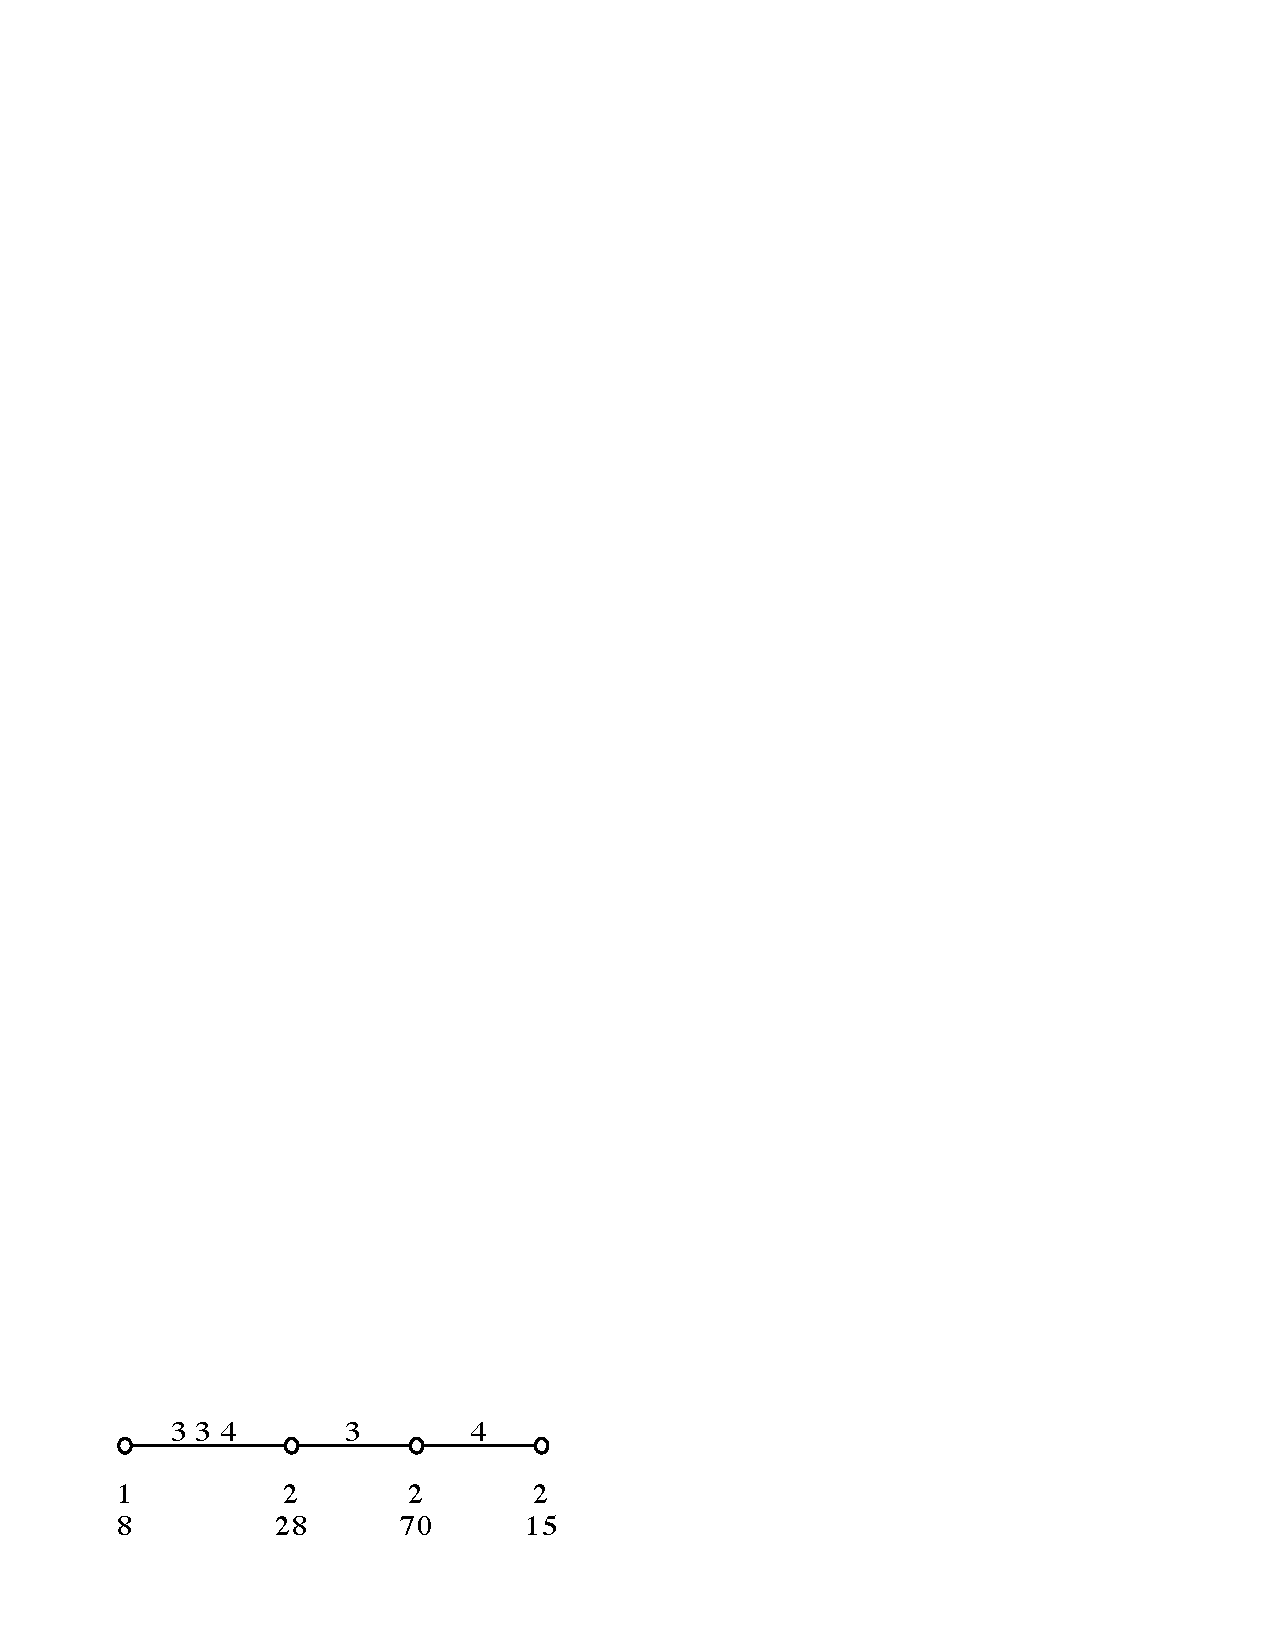
\includegraphics{./graphics/neuma8.pdf}



 The $A_7$ geometry:

 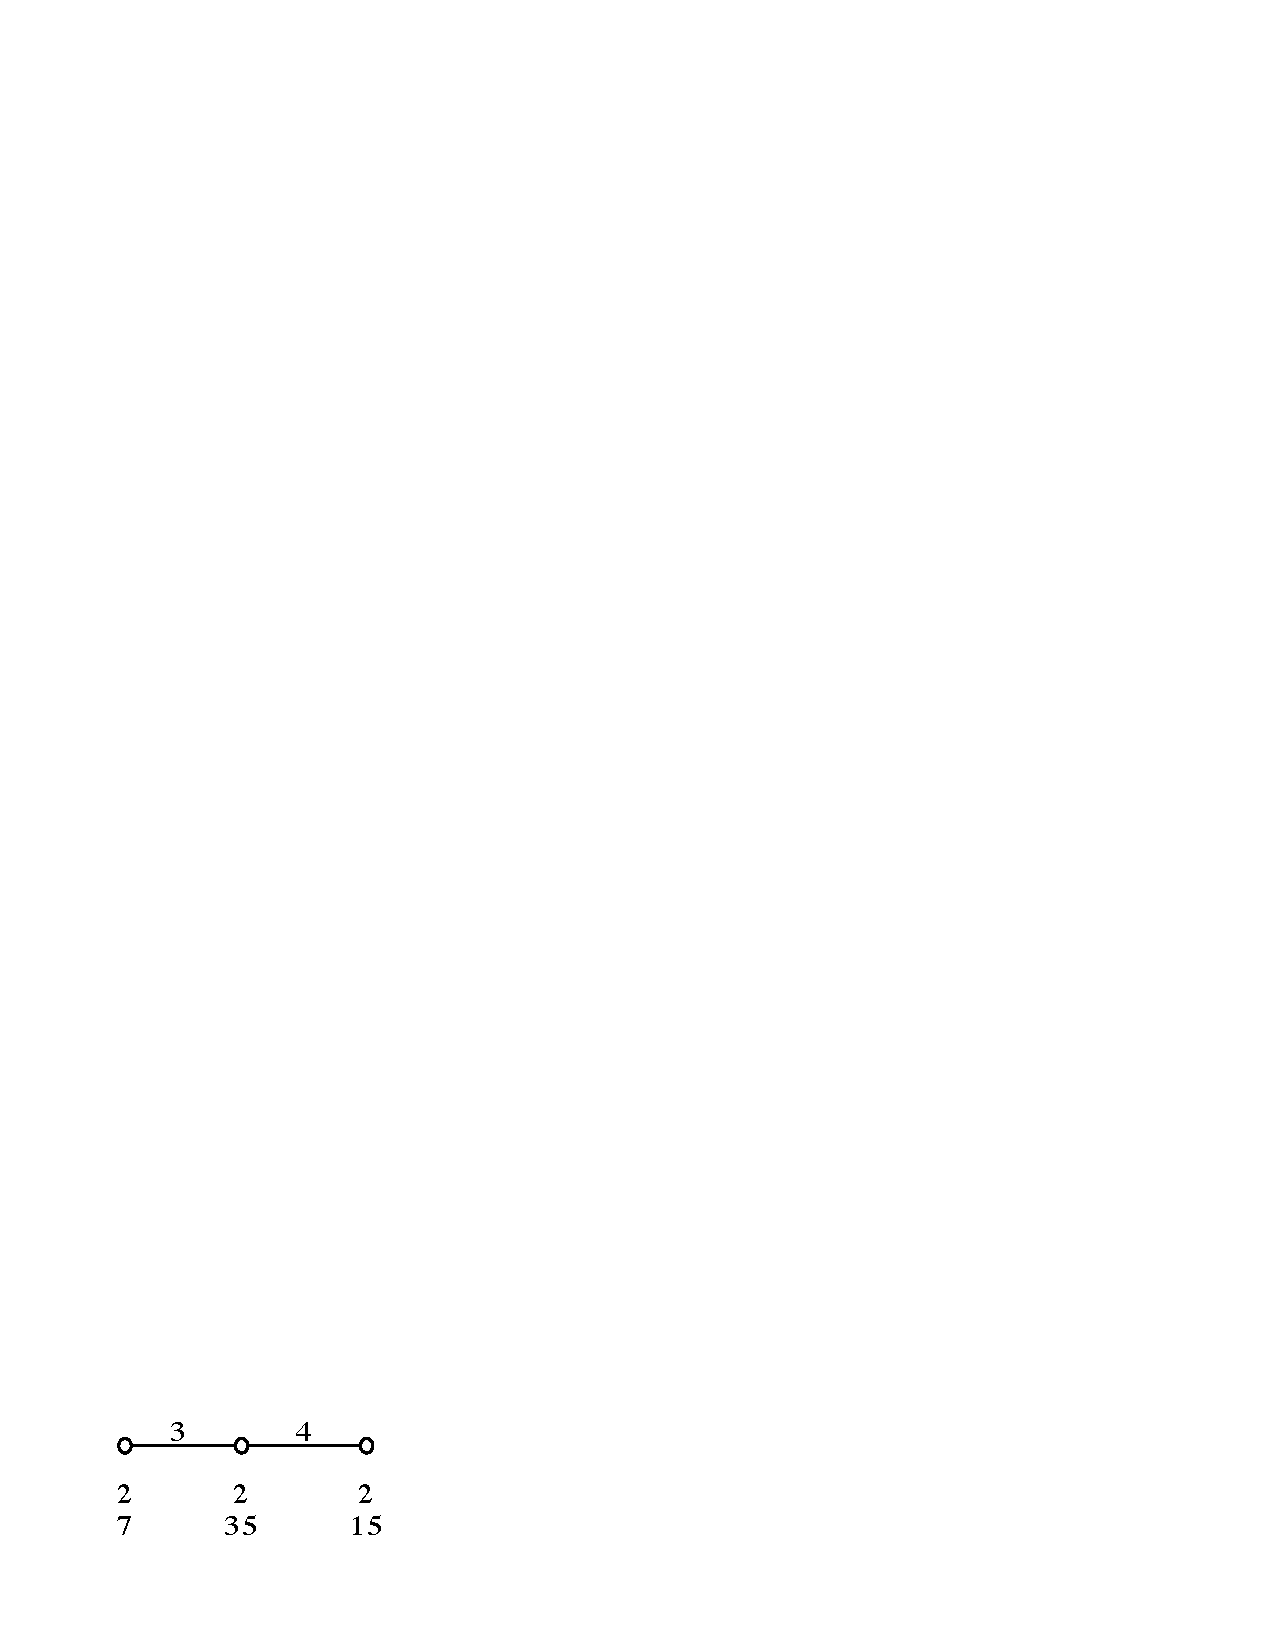
\includegraphics[scale=0.5]{./graphics/a7geo.pdf}



 On a UNIX system we can start an external viewer (``gv'' or ghostview in this
case) from within GAP with the \texttt{Exec} command. 

\subsection{\textcolor{Chapter }{DrawDiagramWithNeato}}
\logpage{[ 13, 3, 4 ]}\nobreak
\hyperdef{L}{X79F882017FEFE4DE}{}
{\noindent\textcolor{FuncColor}{$\triangleright$\ \ \texttt{DrawDiagramWithNeato({\mdseries\slshape diag, filename})\index{DrawDiagramWithNeato@\texttt{DrawDiagramWithNeato}}
\label{DrawDiagramWithNeato}
}\hfill{\scriptsize (operation)}}\\
\textbf{\indent Returns:\ }
does not return anything but writes a file \mbox{\texttt{\mdseries\slshape filename}}.ps



 \mbox{\texttt{\mdseries\slshape diag}} must be a diagram. Writes a file \mbox{\texttt{\mdseries\slshape filename}}.ps in the current directory with a pictorial version of the diagram. 

 This command uses a "spring tension" algorithm to draw the diagram \mbox{\texttt{\mdseries\slshape diag}} with straight edges. For some diagrams this looks better than the result of \texttt{DrawDiagram}. However this algorithm does not print the vertex labels.

 This command uses the \textsf{graphviz} package which is available from http://www.graphviz.org. In case \textsf{graphviz} is not available on your system, you will get an friendly error message and a
file \mbox{\texttt{\mdseries\slshape filename}}.dot will be written. You can then compile this file later or ask a friend to
help you. An $E_6$ geometry for comparison: on the left hand side we have the output of
DrawDiagram and on the right hand side we see the result of
DrawDiagramWithNeato

  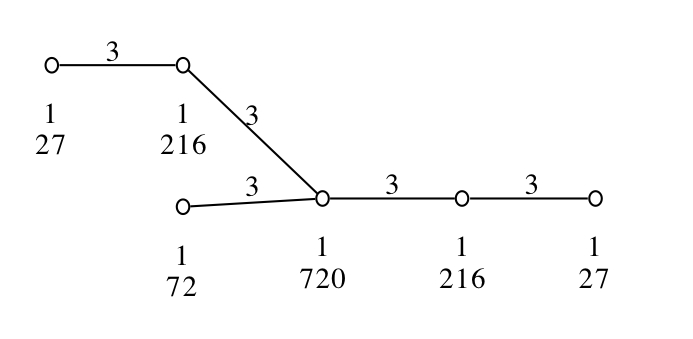
\includegraphics[scale=0.5]{./graphics/E6.jpg}
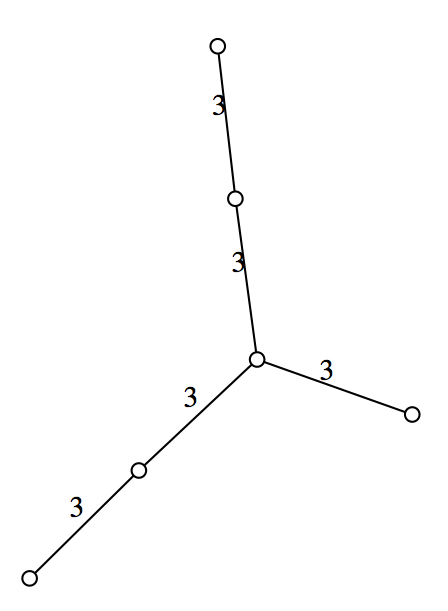
\includegraphics[scale=0.5]{./graphics/E6bis.jpg}



 }

 }

 }

 

\appendix


\chapter{\textcolor{Chapter }{The structure of \textsf{FinInG} }}\label{groups_app}
\logpage{[ "A", 0, 0 ]}
\hyperdef{L}{X86AA009B8756CA64}{}
{
  
\section{\textcolor{Chapter }{The different components}}\logpage{[ "A", 1, 0 ]}
\hyperdef{L}{X84D6D0EC7989CF5E}{}
{
  Loading \textsf{FinInG} shows the following message: 
\begin{Verbatim}[commandchars=!@|,fontsize=\small,frame=single,label=Example]
  ---------------------------------------------------------------------
  loading: geometry, liegeometry, group, projectivespace, correlations, 
  polarspace/morphisms, enumerators, diagram, varieties, affinespace/affinegroup, 
  gpolygons
\end{Verbatim}
 The different components are listed and refer to the corresponding filenames.
So \emph{component} refers to \emph{component.gd} and \emph{component.gi}. When When \emph{component1/component2} is displayed, Both \emph{component1.gi} and \emph{component2.gi} depend on the declarations in both \emph{component1.gd} and \emph{component2.gd}. In other cases, \emph{component{\textunderscore}n} is only dependent on its own declarations and the ones before. }

 
\section{\textcolor{Chapter }{The complete inventory}}\logpage{[ "A", 2, 0 ]}
\hyperdef{L}{X83E153B784E17E05}{}
{
  
\subsection{\textcolor{Chapter }{Declarations}}\logpage{[ "A", 2, 1 ]}
\hyperdef{L}{X844A8A1F85E6E038}{}
{


 
\begin{Verbatim}[commandchars=!@|,fontsize=\small,frame=single,label=Example]
  Operations
  
  geometry.gd: operations
  
  O: IncidenceStructure: [IsList, IsFunction, IsFunction, IsList]
  O: ResidueOfFlag: [IsFlagOfIncidenceStructure]
  O: ElementsOfIncidenceStructure: [IsIncidenceStructure]
  O: ElementsOfIncidenceStructure: [IsIncidenceStructure, IsPosInt]
  O: ElementsOfIncidenceStructure: [IsIncidenceStructure, IsString]
  O: NrElementsOfIncidenceStructure: [IsIncidenceStructure, IsPosInt]
  O: NrElementsOfIncidenceStructure: [IsIncidenceStructure, IsString]
  O: IncidenceGraph: [IsIncidenceStructure]
  O: Points: [IsIncidenceStructure]
  O: Lines: [IsIncidenceStructure]
  O: Planes: [IsIncidenceStructure]
  O: Solids: [IsIncidenceStructure]
  O: FlagOfIncidenceStructure: [IsIncidenceStructure, IsElementOfIncidenceStructureCollection]
  O: FlagOfIncidenceStructure: [IsIncidenceStructure, IsListandIsEmpty]
  O: ChamberOfIncidenceStructure: [IsElementOfIncidenceStructureCollection]
  O: ElementsOfFlag: [IsFlagOfIncidenceStructure]
  O: IsIncident: [IsElementOfIncidenceStructure, IsElementOfIncidenceStructure]
  O: IsIncident: [IsElementOfIncidenceStructure, IsFlagOfIncidenceStructure]
  O: IsIncident: [IsFlagOfIncidenceStructure, IsElementOfIncidenceStructure]
  O: ShadowOfElement: [IsElementOfIncidenceStructure, IsPosInt]
  O: IsCollinear: [IsIncidenceStructure, IsElementOfIncidenceStructure, IsElementOfIncidenceStructure]
  O: Span: [IsElementOfIncidenceStructure, IsElementOfIncidenceStructure]
  O: Meet: [IsElementOfIncidenceStructure, IsElementOfIncidenceStructure]
  O: Type: [IsElementOfIncidenceStructureandIsElementOfIncidenceStructureRep]
  O: Type: [IsElementsOfIncidenceStructureandIsElementsOfIncidenceStructureRep]
  O: Type: [IsFlagOfIncidenceStructureandIsFlagOfIncidenceStructureRep]
  O: Wrap: [IsIncidenceStructure, IsPosInt, IsObject]
  O: Unwrap: [IsElementOfIncidenceStructure]
  O: ObjectToElement: [IsIncidenceStructure, IsPosInt, IsObject]
  O: ObjectToElement: [IsIncidenceStructure, IsObject]
  O: UnderlyingObject: [IsElementOfIncidenceStructure]
  O: ShadowOfElement: [IsIncidenceStructure, IsElementOfIncidenceStructure, IsPosInt]
  O: ShadowOfElement: [IsIncidenceStructure, IsElementOfIncidenceStructure, IsString]
  O: ShadowOfFlag: [IsIncidenceStructure, IsFlagOfIncidenceStructure, IsPosInt]
  O: ShadowOfFlag: [IsIncidenceStructure, IsFlagOfIncidenceStructure, IsString]
  O: ShadowOfFlag: [IsIncidenceStructure, IsList, IsPosInt]
  O: ShadowOfFlag: [IsIncidenceStructure, IsList, IsString]
  O: ElementsIncidentWithElementOfIncidenceStructure: [IsElementOfIncidenceStructure, IsPosInt]
  O: Points: [IsElementOfIncidenceStructure]
  O: Lines: [IsElementOfIncidenceStructure]
  O: Planes: [IsElementOfIncidenceStructure]
  O: Solids: [IsElementOfIncidenceStructure]
  O: Hyperplanes: [IsElementOfIncidenceStructure]
  O: Points: [IsIncidenceStructure, IsElementOfIncidenceStructure]
  O: Lines: [IsIncidenceStructure, IsElementOfIncidenceStructure]
  O: Planes: [IsIncidenceStructure, IsElementOfIncidenceStructure]
  O: Solids: [IsIncidenceStructure, IsElementOfIncidenceStructure]
  O: Hyperplanes: [IsIncidenceStructure, IsElementOfIncidenceStructure]
  
  liegeometry.gd: operations
  
  O: UnderlyingVectorSpace: [IsLieGeometry]
  O: UnderlyingVectorSpace: [IsElementOfLieGeometry]
  O: UnderlyingVectorSpace: [IsFlagOfLieGeometry]
  O: VectorSpaceToElement: [IsLieGeometry, IsRowVector]
  O: VectorSpaceToElement: [IsLieGeometry, Is8BitVectorRep]
  O: VectorSpaceToElement: [IsLieGeometry, IsPlistRep]
  O: VectorSpaceToElement: [IsLieGeometry, Is8BitMatrixRep]
  O: VectorSpaceToElement: [IsLieGeometry, IsGF2MatrixRep]
  O: VectorSpaceToElement: [IsLieGeometry, IsCVecRep]
  O: VectorSpaceToElement: [IsLieGeometry, IsCMatRep]
  O: EmptySubspace: [IsLieGeometry]
  O: RandomSubspace: [IsVectorSpace, IsInt]
  O: IsIncident: [IsEmptySubspace, IsElementOfLieGeometry]
  O: IsIncident: [IsElementOfLieGeometry, IsEmptySubspace]
  O: IsIncident: [IsEmptySubspace, IsLieGeometry]
  O: IsIncident: [IsLieGeometry, IsEmptySubspace]
  O: IsIncident: [IsEmptySubspace, IsEmptySubspace]
  O: Span: [IsEmptySubspace, IsElementOfLieGeometry]
  O: Span: [IsElementOfLieGeometry, IsEmptySubspace]
  O: Span: [IsEmptySubspace, IsLieGeometry]
  O: Span: [IsLieGeometry, IsEmptySubspace]
  O: Span: [IsEmptySubspace, IsEmptySubspace]
  O: Meet: [IsEmptySubspace, IsElementOfLieGeometry]
  O: Meet: [IsElementOfLieGeometry, IsEmptySubspace]
  O: Meet: [IsEmptySubspace, IsLieGeometry]
  O: Meet: [IsLieGeometry, IsEmptySubspace]
  O: Meet: [IsEmptySubspace, IsEmptySubspace]
  O: ElementToElement: [IsLieGeometry, IsElementOfLieGeometry]
  O: ConvertElement: [IsLieGeometry, IsElementOfLieGeometry]
  O: ConvertElementNC: [IsLieGeometry, IsElementOfLieGeometry]
  
  group.gd: operations
  
  O: FindBasePointCandidates: [IsGroup, IsRecord, IsInt]
  O: FindBasePointCandidates: [IsGroup, IsRecord, IsInt, IsObject]
  O: ProjEl: [IsMatrixandIsFFECollColl]
  O: ProjEls: [IsList]
  O: Projectivity: [IsList, IsField]
  O: Projectivity: [IsProjectiveSpace, IsMatrix]
  O: ProjElWithFrob: [IsMatrixandIsFFECollColl, IsMapping]
  O: ProjElWithFrob: [IsMatrixandIsFFECollColl, IsMapping, IsField]
  O: ProjElsWithFrob: [IsList]
  O: ProjElsWithFrob: [IsList, IsField]
  O: CollineationOfProjectiveSpace: [IsList, IsField]
  O: CollineationOfProjectiveSpace: [IsList, IsMapping, IsField]
  O: CollineationOfProjectiveSpace: [IsProjectiveSpace, IsMatrix]
  O: CollineationOfProjectiveSpace: [IsProjectiveSpace, IsMatrix, IsMapping]
  O: Collineation: [IsProjectiveSpace, IsMatrix]
  O: Collineation: [IsProjectiveSpace, IsMatrix, IsMapping]
  O: ProjectiveSemilinearMap: [IsList, IsMapping, IsField]
  O: ProjectivityByImageOfStandardFrameNC: [IsProjectiveSpace, IsList]
  O: MatrixOfCollineation: [IsProjGrpElWithFrobandIsProjGrpElWithFrobRep]
  O: MatrixOfCollineation: [IsProjGrpElandIsProjGrpElRep]
  O: FieldAutomorphism: [IsProjGrpElWithFrobandIsProjGrpElWithFrobRep]
  O: ActionOnAllProjPoints: [IsProjectiveGroupWithFrob]
  O: SetAsNiceMono: [IsProjectiveGroupWithFrob, IsGroupHomomorphism]
  O: CanonicalGramMatrix: [IsString, IsPosInt, IsField]
  O: CanonicalQuadraticForm: [IsString, IsPosInt, IsField]
  O: SOdesargues: [IsInt, IsPosInt, IsFieldandIsFinite]
  O: GOdesargues: [IsInt, IsPosInt, IsFieldandIsFinite]
  O: SUdesargues: [IsPosInt, IsFieldandIsFinite]
  O: GUdesargues: [IsPosInt, IsFieldandIsFinite]
  O: Spdesargues: [IsPosInt, IsFieldandIsFinite]
  O: GeneralSymplecticGroup: [IsPosInt, IsFieldandIsFinite]
  O: GSpdesargues: [IsPosInt, IsFieldandIsFinite]
  O: DeltaOminus: [IsPosInt, IsFieldandIsFinite]
  O: DeltaOplus: [IsPosInt, IsFieldandIsFinite]
  O: GammaOminus: [IsPosInt, IsFieldandIsFinite]
  O: GammaO: [IsPosInt, IsFieldandIsFinite]
  O: GammaOplus: [IsPosInt, IsFieldandIsFinite]
  O: GammaU: [IsPosInt, IsFieldandIsFinite]
  O: GammaSp: [IsPosInt, IsFieldandIsFinite]
  
  projectivespace.gd: operations
  
  O: ProjectiveSpace: [IsInt, IsField]
  O: ProjectiveSpace: [IsInt, IsPosInt]
  O: IsIncident: [IsSubspaceOfProjectiveSpace, IsProjectiveSpace]
  O: IsIncident: [IsProjectiveSpace, IsSubspaceOfProjectiveSpace]
  O: IsIncident: [IsProjectiveSpace, IsProjectiveSpace]
  O: Hyperplanes: [IsProjectiveSpace]
  O: BaerSublineOnThreePoints:   [ IsSubspaceOfProjectiveSpace,  IsSubspaceOfProjectiveSpace,  IsSubspaceOfProjectiveSpace] 
  O: BaerSubplaneOnQuadrangle:   [ IsSubspaceOfProjectiveSpace,  IsSubspaceOfProjectiveSpace,      IsSubspaceOfProjectiveSpace,  IsSubspaceOfProjectiveSpace ] 
  O: RandomSubspace: [IsProjectiveSpace, IsInt]
  O: RandomSubspace: [IsSubspaceOfProjectiveSpace, IsInt]
  O: RandomSubspace: [IsProjectiveSpace]
  O: Span: [IsProjectiveSpace, IsSubspaceOfProjectiveSpace]
  O: Span: [IsSubspaceOfProjectiveSpace, IsProjectiveSpace]
  O: Span: [IsSubspaceOfProjectiveSpace, IsSubspaceOfProjectiveSpace, IsBool]
  O: Span: [IsList]
  O: Span: [IsList, IsBool]
  O: Meet: [IsSubspaceOfProjectiveSpace, IsProjectiveSpace]
  O: Meet: [IsProjectiveSpace, IsSubspaceOfProjectiveSpace]
  O: Meet: [IsList]
  O: DualCoordinatesOfHyperplane: [IsSubspaceOfProjectiveSpace]
  O: HyperplaneByDualCoordinates: [IsProjectiveSpace, IsList]
  O: ComplementSpace: [IsVectorSpace, IsFFECollColl]
  O: ElationOfProjectiveSpace: [IsSubspaceOfProjectiveSpace, IsSubspaceOfProjectiveSpace, IsSubspaceOfProjectiveSpace]
  O: ProjectiveElationGroup: [IsSubspaceOfProjectiveSpace, IsSubspaceOfProjectiveSpace]
  O: ProjectiveElationGroup: [IsSubspaceOfProjectiveSpace]
  O: HomologyOfProjectiveSpace: [IsSubspaceOfProjectiveSpace, IsSubspaceOfProjectiveSpace, IsSubspaceOfProjectiveSpace,  IsSubspaceOfProjectiveSpace ] 
  O: ProjectiveHomologyGroup: [IsSubspaceOfProjectiveSpace, IsSubspaceOfProjectiveSpace]
  
  correlations.gd: operations
  
  O: StandardDualityOfProjectiveSpace: [IsProjectiveSpace]
  O: IdentityMappingOfElementsOfProjectiveSpace: [IsProjectiveSpace]
  O: ActionOnAllPointsHyperplanes: [IsProjGroupWithFrobWithPSIsom]
  O: ProjElWithFrobWithPSIsom:    [IsMatrix and IsFFECollColl,  IsMapping,  IsField] 
  O: ProjElWithFrobWithPSIsom:    [IsMatrix and IsFFECollColl,  IsMapping,  IsField,    IsStandardDualityOfProjectiveSpace] 
  O: ProjElWithFrobWithPSIsom:    [IsMatrix and IsFFECollColl,  IsMapping,  IsField,    IsGeneralMapping and IsSPGeneralMapping and IsOne] 
  O: ProjElsWithFrobWithPSIsom: [IsList, IsField]
  O: SetAsNiceMono:                   [IsProjGroupWithFrobWithPSIsom,  IsGroupHomomorphism] 
  O: CorrelationOfProjectiveSpace: [IsList, IsField]
  O: CorrelationOfProjectiveSpace: [IsList, IsMapping, IsField]
  O: CorrelationOfProjectiveSpace: [IsList, IsField, IsStandardDualityOfProjectiveSpace]
  O: CorrelationOfProjectiveSpace: [IsList, IsField, IsIdentityMappingOfElementsOfProjectiveSpace]
  O: CorrelationOfProjectiveSpace: [IsList, IsMapping, IsField, IsStandardDualityOfProjectiveSpace]
  O: CorrelationOfProjectiveSpace: [IsList, IsMapping, IsField, IsIdentityMappingOfElementsOfProjectiveSpace]
  O: CorrelationOfProjectiveSpace: [IsProjectiveSpace, IsMatrix, IsMapping, IsStandardDualityOfProjectiveSpace]
  O: CorrelationOfProjectiveSpace: [IsProjectiveSpace, IsMatrix, IsMapping, IsIdentityMappingOfElementsOfProjectiveSpace]
  O: Correlation: [IsProjectiveSpace, IsMatrix, IsMapping, IsStandardDualityOfProjectiveSpace]
  O: Correlation: [IsProjectiveSpace, IsMatrix, IsMapping, IsIdentityMappingOfElementsOfProjectiveSpace]
  O: MatrixOfCorrelation: [IsProjGrpElWithFrobWithPSIsomandIsProjGrpElWithFrobWithPSIsomRep]
  O: FieldAutomorphism: [IsProjGrpElWithFrobWithPSIsomandIsProjGrpElWithFrobWithPSIsomRep]
  O: ProjectiveSpaceIsomorphism: [IsProjGrpElWithFrobWithPSIsomandIsProjGrpElWithFrobWithPSIsomRep]
  O: PolarityOfProjectiveSpaceOp: [IsForm]
  O: PolarityOfProjectiveSpace: [IsForm]
  O: PolarityOfProjectiveSpace: [IsMatrix, IsFieldandIsFinite]
  O: PolarityOfProjectiveSpace: [IsMatrix, IsFrobeniusAutomorphism, IsFieldandIsFinite]
  O: HermitianPolarityOfProjectiveSpace: [IsMatrix, IsFieldandIsFinite]
  O: PolarityOfProjectiveSpace: [IsClassicalPolarSpace]
  O: BaseField: [IsPolarityOfProjectiveSpace]
  O: IsAbsoluteElement: [IsElementOfIncidenceStructure, IsPolarityOfProjectiveSpace]
  O: GeometryOfAbsolutePoints: [IsPolarityOfProjectiveSpace]
  O: AbsolutePoints: [IsPolarityOfProjectiveSpace]
  O: PolarSpace: [IsPolarityOfProjectiveSpace]
  
  polarspace.gd: operations
  
  O: PolarSpaceStandard: [IsForm, IsBool]
  O: PolarSpace: [IsForm, IsField, IsGroup, IsFunction]
  O: PolarSpace: [IsForm]
  O: PolarMap: [IsClassicalPolarSpace]
  O: TangentSpace: [IsSubspaceOfClassicalPolarSpace]
  O: TangentSpace: [IsClassicalPolarSpace, IsSubspaceOfProjectiveSpace]
  O: Pole: [IsClassicalPolarSpace, IsSubspaceOfProjectiveSpace]
  O: TypeOfSubspace: [IsClassicalPolarSpace, IsSubspaceOfProjectiveSpace]
  O: CanonicalOrbitRepresentativeForSubspaces: [IsString, IsPosInt, IsField]
  O: RandomSubspace: [IsClassicalPolarSpace, IsPosInt]
  O: NumberOfTotallySingularSubspaces: [IsClassicalPolarSpace, IsPosInt]
  O: EllipticQuadric: [IsPosInt, IsField]
  O: EllipticQuadric: [IsPosInt, IsPosInt]
  O: SymplecticSpace: [IsPosInt, IsField]
  O: SymplecticSpace: [IsPosInt, IsPosInt]
  O: ParabolicQuadric: [IsPosInt, IsField]
  O: ParabolicQuadric: [IsPosInt, IsPosInt]
  O: HyperbolicQuadric: [IsPosInt, IsField]
  O: HyperbolicQuadric: [IsPosInt, IsPosInt]
  O: HermitianPolarSpace: [IsPosInt, IsField]
  O: HermitianPolarSpace: [IsPosInt, IsPosInt]
  O: CanonicalPolarSpace: [IsClassicalPolarSpace]
  O: StandardPolarSpace: [IsClassicalPolarSpace]
  O: Span: [IsSubspaceOfClassicalPolarSpace, IsSubspaceOfClassicalPolarSpace, IsBool]
  
  morphisms.gd: operations
  
  O: GeometryMorphismByFunction:   [ IsAnyElementsOfIncidenceStructure,  IsAnyElementsOfIncidenceStructure,     IsFunction,  IsBool,  IsFunction ] 
  O: GeometryMorphismByFunction:   [ IsAnyElementsOfIncidenceStructure,  IsAnyElementsOfIncidenceStructure,     IsFunction,  IsFunction ] 
  O: GeometryMorphismByFunction:   [ IsAnyElementsOfIncidenceStructure,  IsAnyElementsOfIncidenceStructure,     IsFunction ] 
  O: IsomorphismPolarSpacesProjectionFromNucleus: [IsClassicalPolarSpace, IsClassicalPolarSpace, IsBool]
  O: IsomorphismPolarSpacesNC:  [ IsClassicalPolarSpace,  IsClassicalPolarSpace,  IsBool ]
  O: IsomorphismPolarSpacesNC:                      [ IsClassicalPolarSpace,  IsClassicalPolarSpace ]
  O: IsomorphismPolarSpaces:                      [ IsClassicalPolarSpace,  IsClassicalPolarSpace,  IsBool ]
  O: IsomorphismPolarSpaces:                      [ IsClassicalPolarSpace,  IsClassicalPolarSpace ]
  O: NaturalEmbeddingBySubspace:                      [ IsLieGeometry,  IsLieGeometry,  IsSubspaceOfProjectiveSpace ]
  O: NaturalEmbeddingBySubspaceNC:                      [ IsLieGeometry,  IsLieGeometry,  IsSubspaceOfProjectiveSpace ]
  O: NaturalProjectionBySubspace:                      [ IsClassicalPolarSpace,  IsSubspaceOfClassicalPolarSpace ]
  O: NaturalProjectionBySubspace:                      [ IsProjectiveSpace,  IsSubspaceOfProjectiveSpace ]
  O: NaturalProjectionBySubspaceNC:                      [ IsClassicalPolarSpace,  IsSubspaceOfClassicalPolarSpace ]
  O: NaturalProjectionBySubspaceNC:                      [ IsProjectiveSpace,  IsSubspaceOfProjectiveSpace ]
  O: ShrinkMat: [IsBasis, IsMatrix]
  O: ShrinkMat: [IsField, IsField, IsVector]
  O: ShrinkVec: [IsField, IsField, IsVector]
  O: ShrinkVec: [IsField, IsField, IsVector, IsBasis]
  O: BlownUpProjectiveSpace: [IsBasis, IsProjectiveSpace]
  O: BlownUpProjectiveSpaceBySubfield: [IsField, IsProjectiveSpace]
  O: BlownUpSubspaceOfProjectiveSpace: [IsBasis, IsSubspaceOfProjectiveSpace]
  O: BlownUpSubspaceOfProjectiveSpaceBySubfield: [IsField, IsSubspaceOfProjectiveSpace]
  O: IsDesarguesianSpreadElement: [IsBasis, IsSubspaceOfProjectiveSpace]
  O: IsBlownUpSubspaceOfProjectiveSpace: [IsBasis, IsSubspaceOfProjectiveSpace]
  O: NaturalEmbeddingByFieldReduction:                      [ IsProjectiveSpace,  IsField,  IsBasis ]
  O: NaturalEmbeddingByFieldReduction:                      [ IsProjectiveSpace,  IsField ]
  O: NaturalEmbeddingByFieldReduction:                      [ IsProjectiveSpace,  IsProjectiveSpace ]
  O: NaturalEmbeddingByFieldReduction:                      [ IsProjectiveSpace,  IsProjectiveSpace,  IsBasis ]
  O: BilinearFormFieldReduction: [IsBilinearForm, IsField, IsFFE, IsBasis]
  O: QuadraticFormFieldReduction: [IsQuadraticForm, IsField, IsFFE, IsBasis]
  O: HermitianFormFieldReduction: [IsHermitianForm, IsField, IsFFE, IsBasis]
  O: BilinearFormFieldReduction: [IsBilinearForm, IsField, IsFFE]
  O: QuadraticFormFieldReduction: [IsQuadraticForm, IsField, IsFFE]
  O: HermitianFormFieldReduction: [IsHermitianForm, IsField, IsFFE]
  O: NaturalEmbeddingByFieldReduction: [IsClassicalPolarSpace, IsField, IsFFE, IsBasis, IsBool]
  O: NaturalEmbeddingByFieldReduction: [IsClassicalPolarSpace, IsField, IsFFE, IsBasis]
  O: NaturalEmbeddingByFieldReduction: [IsClassicalPolarSpace, IsField, IsFFE, IsBool]
  O: NaturalEmbeddingByFieldReduction: [IsClassicalPolarSpace, IsField, IsFFE]
  O: NaturalEmbeddingByFieldReduction: [IsClassicalPolarSpace, IsField, IsBool]
  O: NaturalEmbeddingByFieldReduction: [IsClassicalPolarSpace, IsField]
  O: NaturalEmbeddingByFieldReduction: [IsClassicalPolarSpace, IsClassicalPolarSpace, IsBool]
  O: NaturalEmbeddingByFieldReduction: [IsClassicalPolarSpace, IsClassicalPolarSpace]
  O: CanonicalEmbeddingByFieldReduction: [ IsClassicalPolarSpace,  IsField,  IsBool ]
  O: CanonicalEmbeddingByFieldReduction: [ IsClassicalPolarSpace,  IsClassicalPolarSpace,  IsBool ]
  O: NaturalEmbeddingBySubfield:                      [ IsProjectiveSpace,  IsProjectiveSpace ]
  O: NaturalEmbeddingBySubfield:  [ IsClassicalPolarSpace,  IsClassicalPolarSpace,  IsBool ]
  O: NaturalEmbeddingBySubfield:                      [ IsClassicalPolarSpace,  IsClassicalPolarSpace ]
  O: PluckerCoordinates: [IsMatrix]
  O: InversePluckerCoordinates: [IsVector]
  O: PluckerCoordinates: [IsSubspaceOfProjectiveSpace]
  O: KleinCorrespondence: [IsField, IsBool]
  O: KleinCorrespondence: [IsField]
  O: KleinCorrespondence: [IsPosInt, IsBool]
  O: KleinCorrespondence: [IsPosInt]
  O: KleinCorrespondence: [IsClassicalPolarSpace, IsBool]
  O: KleinCorrespondence: [IsClassicalPolarSpace]
  O: KleinCorrespondenceExtended: [IsField, IsBool]
  O: KleinCorrespondenceExtended: [IsField]
  O: KleinCorrespondenceExtended: [IsPosInt, IsBool]
  O: KleinCorrespondenceExtended: [IsPosInt]
  O: KleinCorrespondenceExtended: [IsClassicalPolarSpace, IsBool]
  O: KleinCorrespondenceExtended: [IsClassicalPolarSpace]
  O: NaturalDualitySymplectic: [IsClassicalGQ, IsClassicalGQ, IsBool, IsBool]
  O: NaturalDualityHermitian: [IsClassicalGQ, IsClassicalGQ, IsBool, IsBool]
  O: SelfDualitySymplectic: [IsClassicalGQ, IsBool]
  O: SelfDualityParabolic: [IsClassicalGQ, IsBool]
  O: NaturalDuality: [IsClassicalGQ, IsClassicalGQ, IsBool]
  O: NaturalDuality: [IsClassicalGQ, IsClassicalGQ]
  O: NaturalDuality: [IsClassicalGQ, IsBool]
  O: NaturalDuality: [IsClassicalGQ]
  O: SelfDuality: [IsClassicalGQ, IsBool]
  O: SelfDuality: [IsClassicalGQ]
  O: ProjectiveCompletion: [IsAffineSpace]
  
  enumerators.gd: operations
  
  O: AntonEnumerator: [IsSubspacesOfClassicalPolarSpace]
  O: EnumeratorByOrbit: [IsSubspacesOfClassicalPolarSpace]
  
  diagram.gd: operations
  
  O: CosetGeometry: [IsGroup, IsHomogeneousList]
  O: ParabolicSubgroups: [IsCosetGeometry]
  O: AmbientGroup: [IsCosetGeometry]
  O: FlagToStandardFlag: [IsCosetGeometry, IsFlagOfCosetGeometry]
  O: ResidueOfFlag: [IsFlagOfCosetGeometry]
  O: CanonicalResidueOfFlag: [IsCosetGeometry, IsFlagOfCosetGeometry]
  O: RandomElement: [IsCosetGeometry]
  O: RandomFlag: [IsCosetGeometry]
  O: RandomChamber: [IsCosetGeometry]
  O: AutGroupIncidenceStructureWithNauty: [IsCosetGeometry]
  O: CorGroupIncidenceStructureWithNauty: [IsCosetGeometry]
  O: IsIsomorphicIncidenceStructureWithNauty: [IsCosetGeometry, IsCosetGeometry]
  O: Rk2GeoDiameter: [IsCosetGeometry, IsPosInt]
  O: Rk2GeoGonality: [IsCosetGeometry]
  O: GeometryOfRank2Residue: [IsRank2Residue]
  O: GeometryFromLabelledGraph: [IsObjectandIS_REC]
  O: Rank2Residues: [IsIncidenceGeometry]
  O: MakeRank2Residue: [IsRank2Residue]
  
  varieties.gd: operations
  
  O: AlgebraicVariety: [IsProjectiveSpace, IsList]
  O: AlgebraicVariety: [IsAffineSpace, IsList]
  O: AlgebraicVariety: [IsProjectiveSpace, IsPolynomialRing, IsList]
  O: AlgebraicVariety: [IsAffineSpace, IsPolynomialRing, IsList]
  O: PointsOfAlgebraicVariety: [IsAlgebraicVariety]
  O: Points: [IsAlgebraicVariety]
  O: ProjectiveVariety: [IsProjectiveSpace, IsPolynomialRing, IsList]
  O: ProjectiveVariety: [IsProjectiveSpace, IsList]
  O: HermitianVariety: [IsPosInt, IsField]
  O: HermitianVariety: [IsPosInt, IsPosInt]
  O: HermitianVariety: [IsProjectiveSpace, IsPolynomialRing, IsPolynomial]
  O: HermitianVariety: [IsProjectiveSpace, IsPolynomial]
  O: QuadraticVariety: [IsPosInt, IsField]
  O: QuadraticVariety: [IsPosInt, IsField, IsString]
  O: QuadraticVariety: [IsPosInt, IsPosInt]
  O: QuadraticVariety: [IsPosInt, IsPosInt, IsString]
  O: QuadraticVariety: [IsProjectiveSpace, IsPolynomialRing, IsPolynomial]
  O: QuadraticVariety: [IsProjectiveSpace, IsPolynomial]
  O: PolarSpace: [IsProjectiveVariety]
  O: AffineVariety: [IsAffineSpace, IsPolynomialRing, IsList]
  O: AffineVariety: [IsAffineSpace, IsList]
  O: SegreMap: [IsHomogeneousList]
  O: SegreMap: [IsHomogeneousList, IsField]
  O: SegreVariety: [IsHomogeneousList]
  O: SegreVariety: [IsHomogeneousList, IsField]
  O: PointsOfSegreVariety: [IsSegreVariety]
  O: SegreMap: [IsSegreVariety]
  O: SegreMap: [IsProjectiveSpace, IsProjectiveSpace]
  O: SegreMap: [IsPosInt, IsPosInt, IsField]
  O: SegreMap: [IsPosInt, IsPosInt, IsPosInt]
  O: SegreVariety: [IsProjectiveSpace, IsProjectiveSpace]
  O: SegreVariety: [IsPosInt, IsPosInt, IsField]
  O: SegreVariety: [IsPosInt, IsPosInt, IsPosInt]
  O: VeroneseMap: [IsProjectiveSpace]
  O: VeroneseMap: [IsPosInt, IsField]
  O: VeroneseMap: [IsPosInt, IsPosInt]
  O: VeroneseVariety: [IsProjectiveSpace]
  O: VeroneseVariety: [IsPosInt, IsField]
  O: VeroneseVariety: [IsPosInt, IsPosInt]
  O: PointsOfVeroneseVariety: [IsVeroneseVariety]
  O: VeroneseMap: [IsVeroneseVariety]
  O: GrassmannCoordinates: [IsSubspaceOfProjectiveSpace]
  O: GrassmannMap: [IsPosInt, IsProjectiveSpace]
  O: GrassmannMap: [IsPosInt, IsPosInt, IsPosInt]
  O: GrassmannMap: [IsSubspacesOfProjectiveSpace]
  O: GrassmannMap: [IsGrassmannVariety]
  O: GrassmannVariety: [IsPosInt, IsProjectiveSpace]
  O: GrassmannVariety: [IsPosInt, IsPosInt, IsField]
  O: GrassmannVariety: [IsPosInt, IsPosInt, IsPosInt]
  O: GrassmannVariety: [IsSubspacesOfProjectiveSpace]
  O: PointsOfGrassmannVariety: [IsGrassmannVariety]
  O: ConicOnFivePoints: [IsHomogeneousListand                              IsSubspaceOfProjectiveSpaceCollection ] 
  
  affinespace.gd: operations
  
  O: VectorSpaceTransversal: [IsVectorSpace, IsFFECollColl]
  O: VectorSpaceTransversalElement: [IsVectorSpace, IsFFECollColl, IsVector]
  O: AffineSpace: [IsPosInt, IsField]
  O: AffineSpace: [IsPosInt, IsPosInt]
  O: Hyperplanes: [IsAffineSpace]
  O: AffineSubspace: [IsAffineSpace, IsRowVector]
  O: AffineSubspace: [IsAffineSpace, IsCVecRep]
  O: AffineSubspace: [IsAffineSpace, IsRowVector, IsPlistRep]
  O: AffineSubspace: [IsAffineSpace, IsRowVector, Is8BitMatrixRep]
  O: AffineSubspace: [IsAffineSpace, IsRowVector, IsGF2MatrixRep]
  O: AffineSubspace: [IsAffineSpace, IsCVecRep, IsCMatRep]
  O: RandomSubspace: [IsAffineSpace, IsInt]
  O: IsParallel: [IsSubspaceOfAffineSpace, IsSubspaceOfAffineSpace]
  O: UnderlyingVectorSpace: [IsAffineSpace]
  O: ParallelClass: [IsAffineSpace, IsSubspaceOfAffineSpace]
  O: ParallelClass: [IsSubspaceOfAffineSpace]
  
  affinegroup.gd: operations
  
  
  gpolygons.gd: operations
  
  O: GeneralisedPolygonByBlocks: [IsHomogeneousList]
  O: GeneralisedPolygonByIncidenceMatrix: [IsMatrix]
  O: GeneralisedPolygonByElements: [IsSet, IsSet, IsFunction]
  O: GeneralisedPolygonByElements: [IsSet, IsSet, IsFunction, IsGroup, IsFunction]
  O: DistanceBetweenElements: [IsElementOfGeneralisedPolygon, IsElementOfGeneralisedPolygon]
  O: DistanceBetweenElements: [IsSubspaceOfProjectiveSpace, IsSubspaceOfProjectiveSpace]
  O: BlockDesignOfGeneralisedPolygon: [IsGeneralisedPolygon]
  O: SplitCayleyHexagon: [IsFieldandIsFinite]
  O: SplitCayleyHexagon: [IsPosInt]
  O: SplitCayleyHexagon: [IsClassicalPolarSpace]
  O: TwistedTrialityHexagon: [IsFieldandIsFinite]
  O: TwistedTrialityHexagon: [IsPosInt]
  O: TwistedTrialityHexagon: [IsClassicalPolarSpace]
  O: G2fining: [IsPosInt, IsFieldandIsFinite]
  O: 3D4fining: [IsFieldandIsFinite]
  O: IsKantorFamily: [IsGroup, IsList, IsList]
  O: EGQByKantorFamily: [IsGroup, IsList, IsList]
  O: Wrap: [IsElationGQByKantorFamily, IsPosInt, IsPosInt, IsObject]
  O: IsAnisotropic: [IsFFECollColl, IsFieldandIsFinite]
  O: IsqClan: [IsFFECollCollColl, IsFieldandIsFinite]
  O: qClan: [IsFFECollCollColl, IsField]
  O: LinearqClan: [IsPosInt]
  O: FisherThasWalkerKantorBettenqClan: [IsPosInt]
  O: KantorMonomialqClan: [IsPosInt]
  O: KantorKnuthqClan: [IsPosInt]
  O: FisherqClan: [IsPosInt]
  O: BLTSetByqClan: [IsqClanObjandIsqClanRep]
  O: KantorFamilyByqClan: [IsqClanObjandIsqClanRep]
  O: EGQByqClan: [IsqClanObjandIsqClanRep]
  O: EGQByBLTSet: [IsList, IsSubspaceOfProjectiveSpace, IsSubspaceOfProjectiveSpace]
  O: EGQByBLTSet: [IsList]
  O: FlockGQByqClan: [IsqClanObj]
  
  
\end{Verbatim}
 
\begin{Verbatim}[commandchars=!@|,fontsize=\small,frame=single,label=Example]
  Attributes
  
  geometry.gd: attributes
  
  A: IsChamberOfIncidenceStructure: IsFlagOfIncidenceStructure
  A: IsEmptyFlag: IsFlagOfIncidenceStructure
  A: RankAttr: IsIncidenceStructure
  A: RankAttr: IsFlagOfIncidenceStructure
  A: TypesOfElementsOfIncidenceStructure: IsIncidenceStructure
  A: TypesOfElementsOfIncidenceStructurePlural: IsIncidenceStructure
  A: CollineationGroup: IsIncidenceStructure
  A: CorrelationCollineationGroup: IsIncidenceStructure
  A: CollineationAction: IsIncidenceStructure
  A: CorrelationAction: IsIncidenceStructure
  A: RepresentativesOfElements: IsIncidenceStructure
  A: AmbientGeometry: IsIncidenceStructure
  A: AmbientGeometry: IsFlagOfIncidenceStructure
  A: Size: IsFlagOfIncidenceStructure
  A: AmbientGeometry: IsElementOfIncidenceStructureandIsElementOfIncidenceStructureRep
  A: AmbientGeometry: IsElementsOfIncidenceStructureandIsElementsOfIncidenceStructureRep
  A: AmbientGeometry: IsAllElementsOfIncidenceStructure
  A: CollineationAction: IsGroup
  
  liegeometry.gd: attributes
  
  A: AmbientSpace: IsLieGeometry
  A: AmbientSpace: IsElementOfLieGeometry
  A: ProjectiveDimension: IsLieGeometry
  A: ProjectiveDimension: IsElementOfLieGeometry
  A: ProjectiveDimension: IsEmptySubspace
  A: Dimension: IsLieGeometry
  
  group.gd: attributes
  
  A: Dimension: IsProjectiveGroupWithFrob
  
  projectivespace.gd: attributes
  
  A: ProjectivityGroup: IsProjectiveSpace
  A: SpecialProjectivityGroup: IsProjectiveSpace
  A: Dimension: IsSubspaceOfProjectiveSpace
  A: Dimension: IsEmpty
  A: Coordinates: IsSubspaceOfProjectiveSpace
  A: CoordinatesOfHyperplane: IsSubspaceOfProjectiveSpace
  A: EquationOfHyperplane: IsSubspaceOfProjectiveSpace
  A: StandardFrame: IsProjectiveSpace
  A: StandardFrame: IsSubspaceOfProjectiveSpace
  
  correlations.gd: attributes
  
  A: Dimension: IsProjGroupWithFrobWithPSIsom
  A: GramMatrix: IsPolarityOfProjectiveSpace
  A: CompanionAutomorphism: IsPolarityOfProjectiveSpace
  A: SesquilinearForm: IsPolarityOfProjectiveSpace
  
  polarspace.gd: attributes
  
  A: SesquilinearForm: IsClassicalPolarSpace
  A: QuadraticForm: IsClassicalPolarSpace
  A: AmbientSpace: IsClassicalPolarSpace
  A: SimilarityGroup: IsClassicalPolarSpace
  A: IsometryGroup: IsClassicalPolarSpace
  A: SpecialIsometryGroup: IsClassicalPolarSpace
  A: IsomorphismCanonicalPolarSpace: IsClassicalPolarSpace
  A: IsomorphismCanonicalPolarSpaceWithIntertwiner: IsClassicalPolarSpace
  A: IsCanonicalPolarSpace: IsClassicalPolarSpace
  A: PolarSpaceType: IsClassicalPolarSpace
  A: CompanionAutomorphism: IsClassicalPolarSpace
  A: ClassicalGroupInfo: IsClassicalPolarSpace
  A: EquationForPolarSpace: IsClassicalPolarSpace
  A: NucleusOfParabolicQuadric: IsClassicalPolarSpace
  
  morphisms.gd: attributes
  
  A: Intertwiner: IsGeometryMorphism
  
  enumerators.gd: attributes
  
  
  diagram.gd: attributes
  
  A: DiagramOfGeometry: IsIncidenceGeometry
  A: IsFlagTransitiveGeometry: IsIncidenceGeometry
  A: IsResiduallyConnected: IsIncidenceGeometry
  A: IsConnected: IsIncidenceGeometry
  A: IsFirmGeometry: IsIncidenceGeometry
  A: IsThinGeometry: IsIncidenceGeometry
  A: IsThickGeometry: IsIncidenceGeometry
  A: BorelSubgroup: IsCosetGeometry
  A: StandardFlagOfCosetGeometry: IsCosetGeometry
  A: Rank2Parameters: IsCosetGeometry
  A: OrderVertex: IsVertexOfDiagram
  A: NrElementsVertex: IsVertexOfDiagram
  A: StabiliserVertex: IsVertexOfDiagram
  A: ResidueLabelForEdge: IsEdgeOfDiagram
  A: GirthEdge: IsEdgeOfDiagram
  A: PointDiamEdge: IsEdgeOfDiagram
  A: LineDiamEdge: IsEdgeOfDiagram
  A: ParametersEdge: IsEdgeOfDiagram
  A: GeometryOfDiagram: IsDiagram
  
  varieties.gd: attributes
  
  A: DefiningListOfPolynomials: IsAlgebraicVariety
  A: AmbientSpace: IsAlgebraicVariety
  A: SesquilinearForm: IsHermitianVariety
  A: QuadraticForm: IsQuadraticVariety
  A: Source: IsGeometryMap
  A: Range: IsGeometryMap
  
  affinespace.gd: attributes
  
  A: Dimension: IsAffineSpace
  A: AmbientSpace: IsAffineSpace
  A: AmbientSpace: IsSubspaceOfAffineSpace
  
  affinegroup.gd: attributes
  
  A: AffineGroup: IsAffineSpace
  
  gpolygons.gd: attributes
  
  A: Order: IsGeneralisedPolygon
  A: IncidenceMatrixOfGeneralisedPolygon: IsGeneralisedPolygon
  A: AmbientPolarSpace: IsGeneralisedHexagon
  A: ElationGroup: IsElationGQ
  A: BasePointOfEGQ: IsElationGQ
  A: IsLinearqClan: IsqClanObj
  A: DefiningPlanesOfEGQByBLTSet: IsElationGQByBLTSet
  A: CollineationSubgroup: IsElationGQByBLTSet
  
  
\end{Verbatim}
 
\begin{Verbatim}[commandchars=!@|,fontsize=\small,frame=single,label=Example]
  Properties
  
  geometry.gd: properties
  
  P: IsConfiguration: IsIncidenceStructure
  P: IsConstellation: IsIncidenceStructure
  
  liegeometry.gd: properties
  
  
  group.gd: properties
  
  P: IsProjectivity: IsProjGrpEl
  P: IsProjectivity: IsProjGrpElWithFrob
  P: IsStrictlySemilinear: IsProjGrpEl
  P: IsStrictlySemilinear: IsProjGrpElWithFrob
  P: IsCollineation: IsProjGrpEl
  P: IsCollineation: IsProjGrpElWithFrob
  P: IsProjectivityGroup: IsProjectiveGroupWithFrob
  P: IsCollineationGroup: IsProjectiveGroupWithFrob
  P: CanComputeActionOnPoints: IsProjectiveGroupWithFrob
  
  projectivespace.gd: properties
  
  
  correlations.gd: properties
  
  P: IsCorrelation: IsProjGrpElWithFrobWithPSIsom
  P: IsCorrelation: IsProjGrpElWithFrob
  P: IsCorrelation: IsProjGrpEl
  P: CanComputeActionOnPoints: IsProjGroupWithFrobWithPSIsom
  P: IsProjectivity: IsProjGrpElWithFrobWithPSIsom
  P: IsStrictlySemilinear: IsProjGrpElWithFrobWithPSIsom
  P: IsCollineation: IsProjGrpElWithFrobWithPSIsom
  P: IsProjectivityGroup: IsProjGroupWithFrobWithPSIsom
  P: IsCollineationGroup: IsProjGroupWithFrobWithPSIsom
  P: IsHermitianPolarityOfProjectiveSpace: IsPolarityOfProjectiveSpace
  P: IsSymplecticPolarityOfProjectiveSpace: IsPolarityOfProjectiveSpace
  P: IsOrthogonalPolarityOfProjectiveSpace: IsPolarityOfProjectiveSpace
  P: IsPseudoPolarityOfProjectiveSpace: IsPolarityOfProjectiveSpace
  
  polarspace.gd: properties
  
  P: IsEllipticQuadric: IsClassicalPolarSpace
  P: IsSymplecticSpace: IsClassicalPolarSpace
  P: IsParabolicQuadric: IsClassicalPolarSpace
  P: IsHyperbolicQuadric: IsClassicalPolarSpace
  P: IsHermitianPolarSpace: IsClassicalPolarSpace
  P: IsStandardPolarSpace: IsClassicalPolarSpace
  
  morphisms.gd: properties
  
  
  enumerators.gd: properties
  
  
  diagram.gd: properties
  
  
  varieties.gd: properties
  
  P: IsStandardHermitianVariety: IsHermitianVariety
  P: IsStandardQuadraticVariety: IsQuadraticVariety
  
  affinespace.gd: properties
  
  
  affinegroup.gd: properties
  
  
  gpolygons.gd: properties
  
  P: HasGraphWithUnderlyingObjectsAsVertices: IsGeneralisedPolygon
  
  
\end{Verbatim}
 }

 
\subsection{\textcolor{Chapter }{Functions/Methods}}\logpage{[ "A", 2, 2 ]}
\hyperdef{L}{X81736D4378BF64FF}{}
{


 
\begin{Verbatim}[commandchars=!@|,fontsize=\small,frame=single,label=Example]
  Functions
  
  geometry.gi: global functions
  
  F: HashFuncForElements
  F: HashFuncForSetElements
  
  liegeometry.gi: global functions
  
  
  group.gi: global functions
  
  F: MakeAllProjectivePoints
  F: IsFiningScalarMatrix
  F: OnProjPoints
  F: OnProjPointsWithFrob
  F: OnProjSubspacesNoFrob
  F: OnProjSubspacesWithFrob
  F: NiceMonomorphismByOrbit
  F: NiceMonomorphismByDomain
  
  projectivespace.gi: global functions
  
  F: OnProjSubspaces
  F: OnSetsProjSubspaces
  
  correlations.gi: global functions
  
  F: OnProjPointsWithFrobWithPSIsom
  F: OnProjSubspacesWithFrobWithPSIsom
  F: OnProjSubspacesExtended
  
  polarspace.gi: global functions
  
  
  morphisms.gi: global functions
  
  
  enumerators.gi: global functions
  
  F: PositionNonZeroFromRight
  F: FG_pos
  F: FG_div
  F: FG_ffenumber
  F: FG_alpha_power
  F: FG_log_alpha
  F: FG_beta_power
  F: FG_log_beta
  F: FG_norm_one_element
  F: FG_index_of_norm_one_element
  F: PG_element_normalize
  F: FG_evaluate_hyperbolic_quadratic_form
  F: FG_evaluate_hermitian_form
  F: FG_nb_pts_Nbar
  F: FG_nb_pts_S
  F: FG_nb_pts_N
  F: FG_nb_pts_N1
  F: FG_nb_pts_Sbar
  F: FG_herm_nb_pts_N
  F: FG_herm_nb_pts_S
  F: FG_herm_nb_pts_N1
  F: FG_herm_nb_pts_Sbar
  F: FG_N1_unrank
  F: FG_S_unrank
  F: FG_Sbar_unrank
  F: FG_Nbar_unrank
  F: FG_N_unrank
  F: FG_herm_N_unrank
  F: FG_herm_N_rank
  F: FG_herm_S_unrank
  F: FG_herm_S_rank
  F: FG_herm_N1_unrank
  F: FG_herm_N1_rank
  F: FG_herm_Sbar_unrank
  F: FG_herm_Sbar_rank
  F: FG_S_rank
  F: FG_N_rank
  F: FG_N1_rank
  F: FG_Sbar_rank
  F: FG_Nbar_rank
  F: QElementNumber
  F: QplusElementNumber
  F: QminusElementNumber
  F: QNumberElement
  F: QplusNumberElement
  F: QminusNumberElement
  F: HermElementNumber
  F: HermNumberElement
  F: FG_specialresidual
  F: FG_enum_orthogonal
  F: FG_enum_hermitian
  F: FG_enum_symplectic
  
  diagram.gi: global functions
  
  F: OnCosetGeometryElement
  F: DrawDiagram
  F: DrawDiagramWithNeato
  F: Drawing_Diagram
  
  varieties.gi: global functions
  
  
  affinespace.gi: global functions
  
  
  affinegroup.gi: global functions
  
  F: OnAffinePoints
  F: OnAffineNotPoints
  F: OnAffineSubspaces
  
  gpolygons.gi: global functions
  
  F: SplitCayleyPointToPlane5
  F: SplitCayleyPointToPlane
  F: ZeroPointToOnePointsSpaceByTriality
  F: TwistedTrialityHexagonPointToPlaneByTwoTimesTriality
  F: OnKantorFamily
  
  orbits-stabilisers.gi: global functions
  
  
  
\end{Verbatim}
 
\begin{Verbatim}[commandchars=@|J,fontsize=\small,frame=single,label=Example]
  Methods
  
  geometry.gi: methods
  
  M: IncidenceStructure, [ IsList, IsFunction, IsFunction, IsList ],
  M: Rank, [IsIncidenceStructure],
  M: IncidenceGraph, [ IsIncidenceStructure ],
  M: ElementsOfIncidenceStructure, [IsIncidenceStructure, IsPosInt],
  M: ElementsOfIncidenceStructure, [IsIncidenceStructure, IsString],
  M: Iterator, [ IsElementsOfIncidenceStructure ],
  M: Enumerator, [ IsElementsOfIncidenceStructure ],
  M: NrElementsOfIncidenceStructure, [IsIncidenceStructure, IsString],
  M: NrElementsOfIncidenceStructure, [IsIncidenceStructure, IsPosInt],
  M: ChooseHashFunction, [ IsElementOfIncidenceStructure, IsPosInt ],
  M: ChooseHashFunction, [ CategoryCollections(IsElementOfIncidenceStructure), IsPosInt ],
  M: AmbientGeometry, [ IsElementsOfIncidenceStructure and IsElementsOfIncidenceStructureRep ],
  M: AmbientGeometry, [ IsAllElementsOfIncidenceStructure ],
  M: Type, [IsElementsOfIncidenceStructure and IsElementsOfIncidenceStructureRep],
  M: Wrap, [IsIncidenceStructure, IsPosInt, IsObject],
  M: Unwrap, [IsElementOfIncidenceStructure and IsElementOfIncidenceStructureRep],
  M: UnderlyingObject, [ IsElementOfIncidenceStructure and IsElementOfIncidenceStructureRep ],
  M: ObjectToElement, [ IsIncidenceStructure, IsPosInt, IsObject ],
  M: AmbientGeometry, [ IsElementOfIncidenceStructure and IsElementOfIncidenceStructureRep ],
  M: Intersection2, [IsElementOfIncidenceStructure, IsElementOfIncidenceStructure],
  M: Type, [ IsElementOfIncidenceStructure and IsElementOfIncidenceStructureRep ],
  M: \=, [IsElementOfIncidenceStructure, IsElementOfIncidenceStructure],
  M: \<, [IsElementOfIncidenceStructure, IsElementOfIncidenceStructure],
  M: \*, [IsElementOfIncidenceStructure, IsElementOfIncidenceStructure],
  M: IsIncident, [IsElementOfIncidenceStructure, IsElementOfIncidenceStructure],
  M: FlagOfIncidenceStructure, [ IsIncidenceStructure, IsElementOfIncidenceStructureCollection ],
  M: FlagOfIncidenceStructure, [ IsIncidenceStructure, IsList and IsEmpty ],
  M: IsChamberOfIncidenceStructure, [ IsFlagOfIncidenceStructure and IsFlagOfIncidenceStructureRep ],
  M: AmbientGeometry, [ IsFlagOfIncidenceStructure and IsFlagOfIncidenceStructureRep],
  M: ElementsOfFlag, [ IsFlagOfIncidenceStructure and IsFlagOfIncidenceStructureRep ],
  M: Size, [ IsFlagOfIncidenceStructure and IsFlagOfIncidenceStructureRep ],
  M: Rank, [ IsFlagOfIncidenceStructure ],
  M: Type, [ IsFlagOfIncidenceStructure and IsFlagOfIncidenceStructureRep ],
  M: ResidueOfFlag, [ IsFlagOfIncidenceStructure ],
  M: \=, [ IsFlagOfIncidenceStructure, IsFlagOfIncidenceStructure ],
  M: \<, [ IsFlagOfIncidenceStructure, IsFlagOfIncidenceStructure ],
  M: \<, [ IsFlagOfIncidenceStructure, IsElementOfIncidenceStructure ],
  M: \<, [ IsElementOfIncidenceStructure, IsFlagOfIncidenceStructure ],
  M: IsIncident, [ IsElementOfIncidenceStructure, IsFlagOfIncidenceStructure ],
  M: IsIncident, [IsFlagOfIncidenceStructure, IsElementOfIncidenceStructure],
  M: \in, [ IsElementOfIncidenceStructure, IsFlagOfIncidenceStructure ],
  M: ShadowOfElement, [IsIncidenceStructure, IsElementOfIncidenceStructure, IsPosInt],
  M: ShadowOfElement, [IsIncidenceStructure, IsElementOfIncidenceStructure, IsString],
  M: ElementsIncidentWithElementOfIncidenceStructure, [ IsElementOfIncidenceStructure, IsPosInt],
  M: ShadowOfFlag, [IsIncidenceStructure, IsFlagOfIncidenceStructure, IsPosInt],
  M: ShadowOfFlag, [IsIncidenceStructure, IsFlagOfIncidenceStructure, IsString],
  M: ShadowOfFlag, [IsIncidenceStructure, IsList, IsPosInt],
  M: ShadowOfFlag, [IsIncidenceStructure, IsList, IsString],
  M: Iterator, [ IsShadowElementsOfIncidenceStructure ],
  M: ViewObj, [ IsElementOfIncidenceStructure and IsElementOfIncidenceStructureRep ],
  M: ViewObj, [ IsFlagOfIncidenceStructure and IsFlagOfIncidenceStructureRep ],
  M: PrintObj, [ IsElementOfIncidenceStructure and IsElementOfIncidenceStructureRep ],
  M: Display, [ IsElementOfIncidenceStructure and IsElementOfIncidenceStructureRep ],
  M: ViewObj, [ IsAllElementsOfIncidenceStructure ],
  M: PrintObj, [ IsAllElementsOfIncidenceStructure ],
  M: ViewObj, [ IsShadowElementsOfIncidenceStructure ],
  M: ViewObj, [ IsElementsOfIncidenceStructure ],
  M: PrintObj, [ IsElementsOfIncidenceStructure ],
  M: ViewObj, [ IsIncidenceStructure ],
  M: PrintObj, [ IsIncidenceStructure ],
  M: Display, [ IsIncidenceStructure ],
  M: IsConfiguration, [ IsIncidenceStructure],
  M: IsConstellation, [ IsIncidenceStructure],
  
  liegeometry.gi: methods
  
  M: UnderlyingVectorSpace, [ IsLieGeometry],
  M: ProjectiveDimension, [ IsLieGeometry ],
  M: Dimension, [ IsLieGeometry ],
  M: BaseField, [ IsLieGeometry ],
  M: Wrap, [IsLieGeometry, IsPosInt, IsObject],
  M: UnderlyingObject, [IsElementOfLieGeometry],
  M: AmbientSpace, [IsElementOfLieGeometry],
  M: ViewObj, [ IsAllElementsOfLieGeometry and IsAllElementsOfLieGeometryRep ],
  M: PrintObj, [ IsAllElementsOfLieGeometry and IsAllElementsOfLieGeometryRep ],
  M: ViewObj, [ IsElementsOfLieGeometry and IsElementsOfLieGeometryRep ],
  M: PrintObj, [ IsElementsOfLieGeometry and IsElementsOfLieGeometryRep ],
  M: Points, [IsLieGeometry],
  M: Lines, [IsLieGeometry],
  M: Planes, [IsLieGeometry],
  M: Solids, [IsLieGeometry],
  M: EmptySubspace, [IsLieGeometry],
  M: BaseField, [IsEmptySubspace and IsEmptySubspaceRep],
  M: ViewObj, InstallMethod(ViewObj,[IsEmptySubspace],
  M: PrintObj, InstallMethod(PrintObj,[IsEmptySubspace],
  M: Display, InstallMethod(Display,[IsEmptySubspace],
  M: \=, [IsEmptySubspace, IsEmptySubspace],
  M: \in, [ IsEmptySubspace, IsEmptySubspace ],
  M: \in, [ IsEmptySubspace, IsElementOfLieGeometry ],
  M: \in, [ IsElementOfLieGeometry, IsEmptySubspace ],
  M: \in, [ IsEmptySubspace, IsLieGeometry ],
  M: Span, [ IsEmptySubspace, IsElementOfLieGeometry ],
  M: Span, [ IsElementOfLieGeometry, IsEmptySubspace ],
  M: Span, [IsEmptySubspace, IsEmptySubspace],
  M: Meet, [ IsEmptySubspace, IsElementOfLieGeometry ],
  M: Meet, [ IsElementOfLieGeometry, IsEmptySubspace ],
  M: Meet, [IsEmptySubspace, IsEmptySubspace],
  M: Points, [ IsElementOfLieGeometry ],
  M: Points, [ IsLieGeometry, IsElementOfLieGeometry ],
  M: Lines, [ IsElementOfLieGeometry ],
  M: Lines, [ IsLieGeometry, IsElementOfLieGeometry ],
  M: Planes, [ IsElementOfLieGeometry ],
  M: Planes, [ IsLieGeometry, IsElementOfLieGeometry ],
  M: Solids, InstallMethod(Solids,[IsElementOfLieGeometry],
  M: Solids, [ IsLieGeometry, IsElementOfLieGeometry ],
  M: Hyperplanes, [ IsElementOfLieGeometry ],
  M: Hyperplanes, [ IsLieGeometry, IsElementOfLieGeometry ],
  M: ViewObj, [ IsShadowElementsOfLieGeometry and IsShadowElementsOfLieGeometryRep ],
  M: \in, [IsElementOfLieGeometry, IsElementOfLieGeometry],
  M: Random, [ IsSubspacesVectorSpace ],
  M: RandomSubspace, [IsVectorSpace,IsInt],
  M: ElementToElement, [IsLieGeometry, IsElementOfLieGeometry],
  M: ObjectToElement, [IsLieGeometry, IsPosInt, IsObject],
  M: ObjectToElement, [IsLieGeometry, IsObject],
  
  group.gi: methods
  
  M: ProjEl, [IsMatrix and IsFFECollColl],
  M: ProjEls, [IsList],
  M: Projectivity, InstallMethod(Projectivity,[IsMatrixandIsFFECollColl,IsField],
  M: Projectivity, InstallMethod(Projectivity,[IsCMatRepandIsFFECollColl,IsField],
  M: Projectivity, InstallMethod(Projectivity,[IsProjectiveSpace,IsMatrix],
  M: Projectivity, InstallMethod(Projectivity,[IsProjectiveSpace,IsCMatRep],
  M: IsProjectivity, InstallMethod(IsProjectivity,[IsProjGrpEl],
  M: IsProjectivity, InstallMethod(IsProjectivity,[IsProjGrpElWithFrob],
  M: IsStrictlySemilinear, InstallMethod(IsStrictlySemilinear,[IsProjGrpEl],
  M: IsStrictlySemilinear, InstallMethod(IsStrictlySemilinear,[IsProjGrpElWithFrob],
  M: IsCollineation, InstallMethod(IsCollineation,[IsProjGrpEl],
  M: IsCollineation, InstallMethod(IsCollineation,[IsProjGrpElWithFrob],
  M: IsProjectivityGroup, InstallMethod(IsProjectivityGroup,[IsProjectiveGroupWithFrob],
  M: IsCollineationGroup, InstallMethod(IsCollineationGroup,[IsProjectiveGroupWithFrob],
  M: ProjElWithFrob, [IsCMatRep and IsFFECollColl, #changed 19/3/14 to cmat. IsRingHomomorphism and IsMultiplicativeElementWithInverse, IsField],
  M: ProjElWithFrob, [IsMatrix and IsFFECollColl, IsRingHomomorphism and IsMultiplicativeElementWithInverse, IsField],
  M: ProjElWithFrob, [IsCMatRep and IsFFECollColl, #changed 19/3/14. IsRingHomomorphism and IsMultiplicativeElementWithInverse],
  M: ProjElWithFrob, [IsCMatRep and IsFFECollColl, IsRingHomomorphism and IsMultiplicativeElementWithInverse],
  M: ProjElsWithFrob, [IsList, IsField],
  M: ProjElsWithFrob, [IsList],
  M: CollineationOfProjectiveSpace, [ IsMatrix and IsFFECollColl, IsField],
  M: CollineationOfProjectiveSpace, InstallMethod(CollineationOfProjectiveSpace,[IsProjectiveSpace,IsMatrix],
  M: CollineationOfProjectiveSpace, InstallMethod(CollineationOfProjectiveSpace,[IsProjectiveSpace,IsMatrix,IsMapping],
  M: Collineation, InstallMethod(Collineation,[IsProjectiveSpace,IsMatrix],
  M: Collineation, InstallMethod(Collineation,[IsProjectiveSpace,IsMatrix,IsMapping],
  M: CollineationOfProjectiveSpace, [ IsMatrix and IsFFECollColl, IsRingHomomorphism and IsMultiplicativeElementWithInverse, IsField],
  M: ProjectiveSemilinearMap, [ IsMatrix and IsFFECollColl, IsRingHomomorphism and IsMultiplicativeElementWithInverse, IsField],
  M: ProjectivityByImageOfStandardFrameNC, InstallMethod(ProjectivityByImageOfStandardFrameNC,[IsProjectiveSpace,IsList],
  M: MatrixOfCollineation, InstallMethod(MatrixOfCollineation,[IsProjGrpElandIsProjGrpElRep],
  M: MatrixOfCollineation, InstallMethod(MatrixOfCollineation,[IsProjGrpElWithFrobandIsProjGrpElWithFrobRep],
  M: FieldAutomorphism, InstallMethod(FieldAutomorphism,[IsProjGrpElWithFrobandIsProjGrpElWithFrobRep],
  M: Representative, [IsProjGrpEl and IsProjGrpElRep],
  M: BaseField, [IsProjGrpEl and IsProjGrpElRep],
  M: Representative, [IsProjGrpElWithFrob and IsProjGrpElWithFrobRep],
  M: BaseField, [IsProjGrpElWithFrob and IsProjGrpElWithFrobRep],
  M: ViewObj, [IsProjGrpEl and IsProjGrpElRep],
  M: Display, [IsProjGrpEl and IsProjGrpElRep],
  M: PrintObj, [IsProjGrpEl and IsProjGrpElRep],
  M: ViewObj, [IsProjGrpElWithFrob and IsProjGrpElWithFrobRep],
  M: Display, [IsProjGrpElWithFrob and IsProjGrpElWithFrobRep],
  M: PrintObj, [IsProjGrpElWithFrob and IsProjGrpElWithFrobRep],
  M: \=, [IsProjGrpEl and IsProjGrpElRep, IsProjGrpEl and IsProjGrpElRep],
  M: \<, [IsProjGrpEl, IsProjGrpEl],
  M: \=, [IsProjGrpElWithFrob and IsProjGrpElWithFrobRep, IsProjGrpElWithFrob and IsProjGrpElWithFrobRep],
  M: \<, [IsProjGrpElWithFrob, IsProjGrpElWithFrob],
  M: Order, [IsProjGrpEl and IsProjGrpElRep],
  M: Order, [IsProjGrpElWithFrob and IsProjGrpElWithFrobRep],
  M: IsOne, [IsProjGrpEl and IsProjGrpElRep],
  M: IsOne, [IsProjGrpElWithFrob and IsProjGrpElWithFrobRep],
  M: DegreeFFE, [IsProjGrpEl and IsProjGrpElRep],
  M: DegreeFFE, [IsProjGrpElWithFrob and IsProjGrpElWithFrobRep],
  M: Characteristic, [IsProjGrpEl and IsProjGrpElRep],
  M: Characteristic, [IsProjGrpElWithFrob and IsProjGrpElWithFrobRep],
  M: \*, [IsProjGrpEl and IsProjGrpElRep, IsProjGrpEl and IsProjGrpElRep],
  M: InverseSameMutability, [IsProjGrpEl and IsProjGrpElRep],
  M: InverseMutable, [IsProjGrpEl and IsProjGrpElRep],
  M: OneImmutable, [IsProjGrpEl and IsProjGrpElRep],
  M: OneSameMutability, [IsProjGrpEl and IsProjGrpElRep],
  M: \^, [ IsVector and IsFFECollection and IsMutable, IsFrobeniusAutomorphism ],
  M: \^, [ IsCVecRep and IsFFECollection and IsMutable, IsFrobeniusAutomorphism ],
  M: \^, [ IsVector and IsFFECollection, IsFrobeniusAutomorphism ],
  M: \^, [ IsCVecRep and IsFFECollection, IsFrobeniusAutomorphism ],
  M: \^, [ IsVector and IsFFECollection and IsMutable, IsMapping and IsOne ],
  M: \^, [ IsCVecRep and IsFFECollection and IsMutable, IsMapping and IsOne ],
  M: \^, [ IsVector and IsFFECollection and IsGF2VectorRep, IsFrobeniusAutomorphism ],
  M: \^, [ IsVector and IsFFECollection and IsGF2VectorRep and IsMutable, IsFrobeniusAutomorphism ],
  M: \^, [ IsVector and IsFFECollection and IsGF2VectorRep, IsMapping and IsOne ],
  M: \^, [ IsVector and IsFFECollection and IsGF2VectorRep and IsMutable, IsMapping and IsOne ],
  M: \^, [ IsVector and IsFFECollection and Is8BitVectorRep, IsFrobeniusAutomorphism ],
  M: \^, [ IsVector and IsFFECollection and Is8BitVectorRep and IsMutable, IsFrobeniusAutomorphism ],
  M: \^, [ IsVector and IsFFECollection and Is8BitVectorRep, IsMapping and IsOne ],
  M: \^, [ IsVector and IsFFECollection and Is8BitVectorRep and IsMutable, IsMapping and IsOne ],
  M: \^, [ IsMatrix and IsFFECollColl, IsFrobeniusAutomorphism ],
  M: \^, [ IsCMatRep and IsFFECollColl, IsFrobeniusAutomorphism ],
  M: \^, [ IsMatrix and IsFFECollColl and IsMutable, IsFrobeniusAutomorphism ],
  M: \^, [ IsCMatRep and IsFFECollColl and IsMutable, IsFrobeniusAutomorphism ],
  M: \^, [ IsMatrix and IsFFECollColl, IsMapping and IsOne ],
  M: \^, [ IsCMatRep and IsFFECollColl and IsMutable, IsMapping and IsOne ],
  M: \^, [ IsMatrix and IsFFECollColl, IsMapping and IsOne ],
  M: \^, [ IsCMatRep and IsFFECollColl , IsMapping and IsOne ],
  M: \^, [ IsMatrix and IsFFECollColl and IsGF2MatrixRep, IsFrobeniusAutomorphism ],
  M: \^, [ IsMatrix and IsFFECollColl and IsGF2MatrixRep and IsMutable, IsFrobeniusAutomorphism ],
  M: \^, [ IsMatrix and IsFFECollColl and IsGF2MatrixRep, IsMapping and IsOne ],
  M: \^, [ IsMatrix and IsFFECollColl and IsGF2MatrixRep and IsMutable, IsMapping and IsOne ],
  M: \^, [ IsMatrix and IsFFECollColl and Is8BitMatrixRep, IsFrobeniusAutomorphism ],
  M: \^, [ IsMatrix and IsFFECollColl and Is8BitMatrixRep and IsMutable, IsFrobeniusAutomorphism ],
  M: \^, [ IsMatrix and IsFFECollColl and Is8BitMatrixRep, IsMapping and IsOne ],
  M: \^, [ IsMatrix and IsFFECollColl and Is8BitMatrixRep and IsMutable, IsMapping and IsOne ],
  M: \*, [IsProjGrpElWithFrob and IsProjGrpElWithFrobRep, IsProjGrpElWithFrob and IsProjGrpElWithFrobRep],
  M: InverseSameMutability, [IsProjGrpElWithFrob and IsProjGrpElWithFrobRep],
  M: InverseMutable, [IsProjGrpElWithFrob and IsProjGrpElWithFrobRep],
  M: OneImmutable, [IsProjGrpElWithFrob and IsProjGrpElWithFrobRep],
  M: OneSameMutability, [IsProjGrpElWithFrob and IsProjGrpElWithFrobRep],
  M: ViewObj, [IsProjectiveGroupWithFrob],
  M: ViewObj, [IsProjectiveGroupWithFrob and IsTrivial],
  M: ViewObj, [IsProjectiveGroupWithFrob and HasGeneratorsOfGroup],
  M: ViewObj, [IsProjectiveGroupWithFrob and HasSize],
  M: ViewObj, [IsProjectiveGroupWithFrob and HasGeneratorsOfGroup and HasSize],
  M: BaseField, [IsProjectiveGroupWithFrob],
  M: Dimension, [IsProjectiveGroupWithFrob],
  M: OneImmutable, # was [IsGroup and IsProjectiveGroupWithFrob], I think might be
  M: CanComputeActionOnPoints, [IsProjectiveGroupWithFrob],
  M: ActionOnAllProjPoints, [ IsProjectiveGroupWithFrob ],
  M: SetAsNiceMono, [IsProjectiveGroupWithFrob, IsGroupHomomorphism and IsInjective],
  M: NiceMonomorphism, [IsProjectivityGroup and CanComputeActionOnPoints and IsHandledByNiceMonomorphism],
  M: NiceMonomorphism, [IsProjectiveGroupWithFrob and IsHandledByNiceMonomorphism],
  M: NiceMonomorphism, [IsProjectiveGroupWithFrob and CanComputeActionOnPoints and IsHandledByNiceMonomorphism], 1,
  M: NiceMonomorphism, [IsProjectiveGroupWithFrob and IsHandledByNiceMonomorphism], 50,
  M: FindBasePointCandidates, [IsProjectivityGroup,IsRecord,IsInt],
  M: FindBasePointCandidates, [IsProjectiveGroupWithFrob,IsRecord,IsInt],
  M: FindBasePointCandidates, [IsProjectiveGroupWithFrob,IsRecord,IsInt,IsObject],
  M: CanonicalGramMatrix, [IsString, IsPosInt, IsField],
  M: CanonicalQuadraticForm, [IsString, IsPosInt, IsField],
  M: SOdesargues, [IsInt, IsPosInt, IsField and IsFinite],
  M: GOdesargues, InstallMethod(GOdesargues,[IsInt,IsPosInt,IsFieldandIsFinite],
  M: SUdesargues, InstallMethod(SUdesargues,[IsPosInt,IsFieldandIsFinite],
  M: GUdesargues, InstallMethod(GUdesargues,[IsPosInt,IsFieldandIsFinite],
  M: Spdesargues, InstallMethod(Spdesargues,[IsPosInt,IsFieldandIsFinite],
  M: GeneralSymplecticGroup, InstallMethod(GeneralSymplecticGroup,[IsPosInt,IsFieldandIsFinite],
  M: GSpdesargues, InstallMethod(GSpdesargues,[IsPosInt,IsFieldandIsFinite],
  M: GammaSp, InstallMethod(GammaSp,[IsPosInt,IsFieldandIsFinite],
  M: DeltaOminus, InstallMethod(DeltaOminus,[IsPosInt,IsFieldandIsFinite],
  M: GammaOminus, InstallMethod(GammaOminus,[IsPosInt,IsFieldandIsFinite],
  M: GammaO, InstallMethod(GammaO,[IsPosInt,IsFieldandIsFinite],
  M: DeltaOplus, InstallMethod(DeltaOplus,[IsPosInt,IsFieldandIsFinite],
  M: GammaOplus, InstallMethod(GammaOplus,[IsPosInt,IsFieldandIsFinite],
  M: GammaU, InstallMethod(GammaU,[IsPosInt,IsFieldandIsFinite],
  
  projectivespace.gi: methods
  
  M: Wrap, [IsProjectiveSpace, IsPosInt, IsObject],
  M: ProjectiveSpace, [ IsInt, IsField ],
  M: ProjectiveSpace, [ IsInt, IsPosInt ],
  M: ViewObj, InstallMethod(ViewObj,[IsProjectiveSpaceandIsProjectiveSpaceRep],
  M: ViewString, [ IsProjectiveSpace and IsProjectiveSpaceRep ],
  M: PrintObj, InstallMethod(PrintObj,[IsProjectiveSpaceandIsProjectiveSpaceRep],
  M: Display, InstallMethod(Display,[IsProjectiveSpaceandIsProjectiveSpaceRep],
  M: \=, [IsProjectiveSpace, IsProjectiveSpace],
  M: Rank, [ IsProjectiveSpace and IsProjectiveSpaceRep ],
  M: BaseField, [IsSubspaceOfProjectiveSpace],
  M: StandardFrame, [IsProjectiveSpace],
  M: RepresentativesOfElements, "for a projective space", [IsProjectiveSpace],
  M: Hyperplanes, [ IsProjectiveSpace ],
  M: TypesOfElementsOfIncidenceStructure, "for a projective space", [IsProjectiveSpace],
  M: TypesOfElementsOfIncidenceStructurePlural, [IsProjectiveSpace],
  M: ElementsOfIncidenceStructure, [IsProjectiveSpace, IsPosInt],
  M: ElementsOfIncidenceStructure, [IsProjectiveSpace],
  M: \=, [ IsAllSubspacesOfProjectiveSpace, IsAllSubspacesOfProjectiveSpace ],
  M: Size, [IsSubspacesOfProjectiveSpace and IsSubspacesOfProjectiveSpaceRep],
  M: \in, [IsElementOfIncidenceStructure, IsElementsOfIncidenceStructure], 1*SUM_FLAGS+3,
  M: \in, [IsElementOfIncidenceStructure, IsAllElementsOfIncidenceStructure], 1*SUM_FLAGS+3,
  M: VectorSpaceToElement, [IsProjectiveSpace, IsCMatRep],
  M: VectorSpaceToElement, [IsProjectiveSpace, IsPlistRep],
  M: VectorSpaceToElement, [IsProjectiveSpace, IsGF2MatrixRep],
  M: VectorSpaceToElement, [IsProjectiveSpace, Is8BitMatrixRep],
  M: VectorSpaceToElement, [IsProjectiveSpace, IsCVecRep],
  M: VectorSpaceToElement, [IsProjectiveSpace, IsRowVector],
  M: VectorSpaceToElement, [IsProjectiveSpace, Is8BitVectorRep],
  M: UnderlyingVectorSpace, [IsSubspaceOfProjectiveSpace],
  M: ProjectiveDimension, [ IsSubspaceOfProjectiveSpace ],
  M: Dimension, [ IsSubspaceOfProjectiveSpace ],
  M: StandardFrame, [IsSubspaceOfProjectiveSpace],
  M: Coordinates, [IsSubspaceOfProjectiveSpace],
  M: DualCoordinatesOfHyperplane, [IsSubspaceOfProjectiveSpace],
  M: HyperplaneByDualCoordinates, [IsProjectiveSpace,IsList],
  M: EquationOfHyperplane, [IsSubspaceOfProjectiveSpace],
  M: Span, [ IsEmptySubspace, IsProjectiveSpace ],
  M: Span, [ IsProjectiveSpace, IsEmptySubspace ],
  M: Meet, [ IsEmptySubspace, IsProjectiveSpace ],
  M: Meet, [ IsProjectiveSpace, IsEmptySubspace ],
  M: ShadowOfElement, [IsProjectiveSpace, IsSubspaceOfProjectiveSpace, IsPosInt],
  M: Size, [IsShadowSubspacesOfProjectiveSpace and IsShadowSubspacesOfProjectiveSpaceRep ],
  M: CollineationGroup, [ IsProjectiveSpace and IsProjectiveSpaceRep ],
  M: ProjectivityGroup, [ IsProjectiveSpace ],
  M: SpecialProjectivityGroup, [ IsProjectiveSpace ],
  M: \^, [IsElementOfIncidenceStructure, IsProjGrpElWithFrob],
  M: \^, [IsElementOfIncidenceStructure, IsProjGrpElWithFrobWithPSIsom],
  M: AsList, [IsSubspacesOfProjectiveSpace],
  M: Iterator, [IsSubspacesOfProjectiveSpace],
  M: FlagOfIncidenceStructure, [ IsProjectiveSpace, IsSubspaceOfProjectiveSpaceCollection ],
  M: FlagOfIncidenceStructure, [ IsProjectiveSpace, IsList and IsEmpty ],
  M: UnderlyingVectorSpace, [ IsFlagOfProjectiveSpace and IsFlagOfIncidenceStructureRep ],
  M: ViewObj, [ IsFlagOfProjectiveSpace and IsFlagOfIncidenceStructureRep ],
  M: PrintObj, [ IsFlagOfProjectiveSpace and IsFlagOfIncidenceStructureRep ],
  M: Display, [ IsFlagOfProjectiveSpace and IsFlagOfIncidenceStructureRep ],
  M: ShadowOfFlag, [IsProjectiveSpace, IsFlagOfProjectiveSpace, IsPosInt],
  M: Iterator, [IsShadowSubspacesOfProjectiveSpace and IsShadowSubspacesOfProjectiveSpaceRep ],
  M: \in, [ IsProjectiveSpace, IsSubspaceOfProjectiveSpace ],
  M: \in, [ IsProjectiveSpace, IsEmptySubspace ],
  M: \in, [IsSubspaceOfProjectiveSpace, IsProjectiveSpace],
  M: \in, [IsProjectiveSpace, IsSubspaceOfProjectiveSpace],
  M: IsIncident, [IsSubspaceOfProjectiveSpace, IsSubspaceOfProjectiveSpace],
  M: Span, [IsProjectiveSpace, IsSubspaceOfProjectiveSpace],
  M: Span, [IsSubspaceOfProjectiveSpace, IsProjectiveSpace],
  M: Span, [IsSubspaceOfProjectiveSpace, IsSubspaceOfProjectiveSpace],
  M: Span, [IsSubspaceOfProjectiveSpace, IsSubspaceOfProjectiveSpace, IsBool],
  M: Span, [ IsHomogeneousList and IsSubspaceOfProjectiveSpaceCollection ],
  M: Span, [ IsList ],
  M: Span, [IsList, IsBool],
  M: Meet, [IsProjectiveSpace, IsSubspaceOfProjectiveSpace],
  M: Meet, [IsSubspaceOfProjectiveSpace, IsProjectiveSpace],
  M: Meet, [IsSubspaceOfProjectiveSpace, IsSubspaceOfProjectiveSpace],
  M: Meet, [ IsHomogeneousList and IsSubspaceOfProjectiveSpaceCollection],
  M: Meet, [ IsList ],
  M: RandomSubspace, [IsProjectiveSpace,IsInt],
  M: RandomSubspace, [IsSubspaceOfProjectiveSpace,IsInt],
  M: RandomSubspace, [IsProjectiveSpace],
  M: Random, [ IsSubspacesOfProjectiveSpace ],
  M: Random, [ IsAllSubspacesOfProjectiveSpace ],
  M: Random, [ IsShadowSubspacesOfProjectiveSpace ],
  M: BaerSublineOnThreePoints, [IsSubspaceOfProjectiveSpace, IsSubspaceOfProjectiveSpace, IsSubspaceOfProjectiveSpace],
  M: BaerSubplaneOnQuadrangle, InstallMethod(BaerSubplaneOnQuadrangle,[IsSubspaceOfProjectiveSpace, IsSubspaceOfProjectiveSpace, IsSubspaceOfProjectiveSpace, IsSubspaceOfProjectiveSpace],
  M: ComplementSpace, [IsVectorSpace, IsFFECollColl],
  M: ElationOfProjectiveSpace, [ IsSubspaceOfProjectiveSpace, IsSubspaceOfProjectiveSpace, IsSubspaceOfProjectiveSpace ],
  M: ProjectiveElationGroup, [ IsSubspaceOfProjectiveSpace, IsSubspaceOfProjectiveSpace ],
  M: ProjectiveElationGroup, [ IsSubspaceOfProjectiveSpace ],
  M: HomologyOfProjectiveSpace, [ IsSubspaceOfProjectiveSpace, IsSubspaceOfProjectiveSpace, IsSubspaceOfProjectiveSpace, IsSubspaceOfProjectiveSpace ],
  M: ProjectiveHomologyGroup, [ IsSubspaceOfProjectiveSpace, IsSubspaceOfProjectiveSpace ],
  M: IncidenceGraph, [ IsProjectiveSpace ],
  
  correlations.gi: methods
  
  M: IdentityMappingOfElementsOfProjectiveSpace, [IsProjectiveSpace],
  M: StandardDualityOfProjectiveSpace, [IsProjectiveSpace],
  M: IsCollineation, InstallMethod(IsCollineation,[IsProjGrpElWithFrobWithPSIsom],
  M: IsCorrelation, InstallMethod(IsCorrelation,[IsProjGrpElWithFrobWithPSIsom],
  M: IsCorrelation, InstallMethod(IsCorrelation,[IsProjGrpElWithFrob],
  M: IsCorrelation, InstallMethod(IsCorrelation,[IsProjGrpEl],
  M: IsProjectivity, [ IsProjGrpElWithFrobWithPSIsom and IsProjGrpElWithFrobWithPSIsomRep],
  M: IsStrictlySemilinear, [ IsProjGrpElWithFrobWithPSIsom and IsProjGrpElWithFrobWithPSIsomRep],
  M: IsProjectivityGroup, InstallMethod(IsProjectivityGroup,[IsProjGroupWithFrobWithPSIsom],
  M: IsCollineationGroup, InstallMethod(IsCollineationGroup,[IsProjGroupWithFrobWithPSIsom],
  M: ViewObj, [IsStandardDualityOfProjectiveSpace and IsSPMappingByFunctionWithInverseRep],
  M: Display, [IsStandardDualityOfProjectiveSpace and IsSPMappingByFunctionWithInverseRep],
  M: PrintObj, [IsStandardDualityOfProjectiveSpace and IsSPMappingByFunctionWithInverseRep],
  M: \*, [IsStandardDualityOfProjectiveSpace, IsStandardDualityOfProjectiveSpace],
  M: \*, [IsIdentityMappingOfElementsOfProjectiveSpace, IsStandardDualityOfProjectiveSpace],
  M: \*, [IsStandardDualityOfProjectiveSpace, IsIdentityMappingOfElementsOfProjectiveSpace],
  M: \*, [IsIdentityMappingOfElementsOfProjectiveSpace, IsIdentityMappingOfElementsOfProjectiveSpace],
  M: \^, [ IsProjectiveSpaceIsomorphism, IsZeroCyc ],
  M: \=, [IsStandardDualityOfProjectiveSpace, IsStandardDualityOfProjectiveSpace],
  M: \=, [IsStandardDualityOfProjectiveSpace, IsIdentityMappingOfElementsOfProjectiveSpace],
  M: \=, [IsIdentityMappingOfElementsOfProjectiveSpace, IsStandardDualityOfProjectiveSpace],
  M: \=, [IsIdentityMappingOfElementsOfProjectiveSpace, IsIdentityMappingOfElementsOfProjectiveSpace],
  M: ProjElWithFrobWithPSIsom, [IsCMatRep and IsFFECollColl, IsRingHomomorphism and IsMultiplicativeElementWithInverse, IsField, IsStandardDualityOfProjectiveSpace],
  M: ProjElWithFrobWithPSIsom, [IsMatrix and IsFFECollColl, IsRingHomomorphism and IsMultiplicativeElementWithInverse, IsField, IsStandardDualityOfProjectiveSpace],
  M: ProjElWithFrobWithPSIsom, [IsCMatRep and IsFFECollColl, IsRingHomomorphism and IsMultiplicativeElementWithInverse, IsField],
  M: ProjElWithFrobWithPSIsom, [IsMatrix and IsFFECollColl, IsRingHomomorphism and IsMultiplicativeElementWithInverse, IsField],
  M: ProjElWithFrobWithPSIsom, [IsCMatRep and IsFFECollColl, IsRingHomomorphism and IsMultiplicativeElementWithInverse, IsField, IsGeneralMappingand IsSPGeneralMapping and IsOne],
  M: ProjElWithFrobWithPSIsom, [IsMatrix and IsFFECollColl, IsRingHomomorphism and IsMultiplicativeElementWithInverse, IsField, IsGeneralMappingand IsSPGeneralMapping and IsOne],
  M: ViewObj, [IsProjGrpElWithFrobWithPSIsom and IsProjGrpElWithFrobWithPSIsomRep],
  M: Display, [IsProjGrpElWithFrobWithPSIsom and IsProjGrpElWithFrobWithPSIsomRep],
  M: PrintObj, [IsProjGrpElWithFrobWithPSIsom and IsProjGrpElWithFrobWithPSIsomRep],
  M: Representative, [IsProjGrpElWithFrobWithPSIsom and IsProjGrpElWithFrobWithPSIsomRep],
  M: BaseField, [IsProjGrpElWithFrobWithPSIsom and IsProjGrpElWithFrobWithPSIsomRep],
  M: BaseField, [IsProjGroupWithFrobWithPSIsom],
  M: \=, [IsProjGrpElWithFrobWithPSIsom and IsProjGrpElWithFrobWithPSIsomRep, IsProjGrpElWithFrobWithPSIsom and IsProjGrpElWithFrobWithPSIsomRep],
  M: IsOne, [IsProjGrpElWithFrobWithPSIsom and IsProjGrpElWithFrobWithPSIsomRep],
  M: OneImmutable, [IsProjGrpElWithFrobWithPSIsom and IsProjGrpElWithFrobWithPSIsomRep],
  M: OneImmutable, [IsGroup and IsProjGrpElWithFrobWithPSIsom],
  M: OneSameMutability, [IsProjGrpElWithFrobWithPSIsom and IsProjGrpElWithFrobWithPSIsomRep],
  M: \^, [ IsCVecRep and IsFFECollection, IsIdentityMappingOfElementsOfProjectiveSpace ],
  M: \^, [ IsVector and IsFFECollection, IsIdentityMappingOfElementsOfProjectiveSpace ],
  M: \^, [ IsVector and IsFFECollection and IsGF2VectorRep, IsIdentityMappingOfElementsOfProjectiveSpace ],
  M: \^, [ IsVector and IsFFECollection and Is8BitVectorRep, IsIdentityMappingOfElementsOfProjectiveSpace ],
  M: \^, [ IsCMatRep and IsFFECollColl, IsStandardDualityOfProjectiveSpace ],
  M: \^, [ IsMatrix and IsFFECollColl, IsStandardDualityOfProjectiveSpace ],
  M: \^, [ IsCMatRep and IsFFECollColl, IsIdentityMappingOfElementsOfProjectiveSpace ],
  M: \^, [ IsMatrix and IsFFECollColl, IsIdentityMappingOfElementsOfProjectiveSpace ],
  M: \^, [ IsSubspaceOfProjectiveSpace, IsIdentityMappingOfElementsOfProjectiveSpace ],
  M: \^, [ IsSubspaceOfProjectiveSpace, IsStandardDualityOfProjectiveSpace ],
  M: \*, [IsProjGrpElWithFrobWithPSIsom and IsProjGrpElWithFrobWithPSIsomRep, IsProjGrpElWithFrobWithPSIsom and IsProjGrpElWithFrobWithPSIsomRep],
  M: \<, [IsProjGrpElWithFrobWithPSIsom, IsProjGrpElWithFrobWithPSIsom],
  M: InverseSameMutability, [IsProjGrpElWithFrobWithPSIsom and IsProjGrpElWithFrobWithPSIsomRep],
  M: InverseMutable, [IsProjGrpElWithFrobWithPSIsom and IsProjGrpElWithFrobWithPSIsomRep],
  M: \*, [IsProjGrpElWithFrob and IsProjGrpElWithFrobRep, IsProjGrpElWithFrobWithPSIsom and IsProjGrpElWithFrobWithPSIsomRep],
  M: \*, [IsProjGrpElWithFrobWithPSIsom and IsProjGrpElWithFrobWithPSIsomRep, IsProjGrpElWithFrob and IsProjGrpElWithFrobRep],
  M: ProjElsWithFrobWithPSIsom, [IsList, IsField],
  M: CorrelationCollineationGroup, [ IsProjectiveSpace and IsProjectiveSpaceRep ],
  M: CorrelationOfProjectiveSpace, [ IsMatrix and IsFFECollColl, IsField],
  M: CorrelationOfProjectiveSpace, [ IsMatrix and IsFFECollColl, IsRingHomomorphism and IsMultiplicativeElementWithInverse, IsField],
  M: CorrelationOfProjectiveSpace, [ IsMatrix and IsFFECollColl, IsField, IsStandardDualityOfProjectiveSpace],
  M: CorrelationOfProjectiveSpace, [ IsMatrix and IsFFECollColl, IsField, IsIdentityMappingOfElementsOfProjectiveSpace],
  M: CorrelationOfProjectiveSpace, [ IsMatrix and IsFFECollColl, IsRingHomomorphism and IsMultiplicativeElementWithInverse, IsField, IsStandardDualityOfProjectiveSpace],
  M: CorrelationOfProjectiveSpace, [ IsMatrix and IsFFECollColl, IsRingHomomorphism and IsMultiplicativeElementWithInverse, IsField, IsIdentityMappingOfElementsOfProjectiveSpace],
  M: CorrelationOfProjectiveSpace, [ IsProjectiveSpace, IsMatrix and IsFFECollColl, IsRingHomomorphism and IsMultiplicativeElementWithInverse, IsStandardDualityOfProjectiveSpace],
  M: CorrelationOfProjectiveSpace, [ IsProjectiveSpace, IsMatrix and IsFFECollColl, IsRingHomomorphism and IsMultiplicativeElementWithInverse, IsIdentityMappingOfElementsOfProjectiveSpace],
  M: Correlation, [ IsProjectiveSpace, IsMatrix and IsFFECollColl, IsRingHomomorphism and IsMultiplicativeElementWithInverse, IsStandardDualityOfProjectiveSpace],
  M: Correlation, [ IsProjectiveSpace, IsMatrix and IsFFECollColl, IsRingHomomorphism and IsMultiplicativeElementWithInverse, IsIdentityMappingOfElementsOfProjectiveSpace],
  M: MatrixOfCorrelation, InstallMethod(MatrixOfCorrelation,[IsProjGrpElWithFrobWithPSIsomand IsProjGrpElWithFrobWithPSIsomRep],
  M: FieldAutomorphism, InstallMethod(FieldAutomorphism,[IsProjGrpElWithFrobWithPSIsomand IsProjGrpElWithFrobWithPSIsomRep],
  M: ProjectiveSpaceIsomorphism, InstallMethod(ProjectiveSpaceIsomorphism,[IsProjGrpElWithFrobWithPSIsomand IsProjGrpElWithFrobWithPSIsomRep],
  M: Embedding, [IsProjectiveGroupWithFrob, IsProjGroupWithFrobWithPSIsom],
  M: Dimension, [IsProjGroupWithFrobWithPSIsom],
  M: ActionOnAllPointsHyperplanes, [ IsProjGroupWithFrobWithPSIsom ],
  M: CanComputeActionOnPoints, [IsProjGroupWithFrobWithPSIsom],
  M: SetAsNiceMono, [IsProjGroupWithFrobWithPSIsom, IsGroupHomomorphism and IsInjective],
  M: NiceMonomorphism, [IsProjGroupWithFrobWithPSIsom and CanComputeActionOnPoints and IsHandledByNiceMonomorphism], 50,
  M: NiceMonomorphism, [IsProjGroupWithFrobWithPSIsom and IsHandledByNiceMonomorphism], 50,
  M: ViewObj, [IsProjGroupWithFrobWithPSIsom],
  M: ViewObj, [IsProjGroupWithFrobWithPSIsom and IsTrivial],
  M: ViewObj, [IsProjGroupWithFrobWithPSIsom and HasGeneratorsOfGroup],
  M: ViewObj, [IsProjGroupWithFrobWithPSIsom and HasSize],
  M: ViewObj, [IsProjGroupWithFrobWithPSIsom and HasGeneratorsOfGroup and HasSize],
  M: PolarityOfProjectiveSpaceOp, [IsSesquilinearForm and IsFormRep],
  M: ViewObj, [IsPolarityOfProjectiveSpace and IsPolarityOfProjectiveSpaceRep],
  M: PrintObj, [IsPolarityOfProjectiveSpace and IsPolarityOfProjectiveSpaceRep],
  M: Display, [IsPolarityOfProjectiveSpace and IsPolarityOfProjectiveSpaceRep],
  M: PolarityOfProjectiveSpace, [IsSesquilinearForm and IsFormRep],
  M: PolarityOfProjectiveSpace, [IsMatrix,IsField and IsFinite],
  M: PolarityOfProjectiveSpace, [IsMatrix, IsFrobeniusAutomorphism, IsField and IsFinite],
  M: HermitianPolarityOfProjectiveSpace, [IsMatrix,IsField and IsFinite],
  M: GramMatrix, [IsPolarityOfProjectiveSpace and IsPolarityOfProjectiveSpaceRep],
  M: BaseField, [IsPolarityOfProjectiveSpace and IsPolarityOfProjectiveSpaceRep],
  M: CompanionAutomorphism, [IsPolarityOfProjectiveSpace and IsPolarityOfProjectiveSpaceRep],
  M: SesquilinearForm, [IsPolarityOfProjectiveSpace and IsPolarityOfProjectiveSpaceRep],
  M: IsHermitianPolarityOfProjectiveSpace, [IsPolarityOfProjectiveSpace and IsPolarityOfProjectiveSpaceRep],
  M: IsOrthogonalPolarityOfProjectiveSpace, [IsPolarityOfProjectiveSpace and IsPolarityOfProjectiveSpaceRep],
  M: IsSymplecticPolarityOfProjectiveSpace, [IsPolarityOfProjectiveSpace and IsPolarityOfProjectiveSpaceRep],
  M: IsPseudoPolarityOfProjectiveSpace, [IsPolarityOfProjectiveSpace and IsPolarityOfProjectiveSpaceRep],
  M: \^, [ IsSubspaceOfProjectiveSpace, IsPolarityOfProjectiveSpace],
  
  polarspace.gi: methods
  
  M: Wrap, [IsClassicalPolarSpace, IsPosInt, IsObject],
  M: PolarSpace, [ IsSesquilinearForm, IsField, IsGroup, IsFunction ],
  M: PolarSpaceStandard, [ IsSesquilinearForm, IsBool ],
  M: PolarSpaceStandard, [ IsQuadraticForm, IsBool ],
  M: PolarSpace, [ IsSesquilinearForm ],
  M: PolarSpace, [ IsQuadraticForm ],
  M: PolarSpace, [ IsHermitianForm ],
  M: CanonicalOrbitRepresentativeForSubspaces, [IsString, IsPosInt, IsField],
  M: EllipticQuadric, [ IsPosInt, IsField ],
  M: EllipticQuadric, [ IsPosInt, IsPosInt ],
  M: SymplecticSpace, [ IsPosInt, IsField ],
  M: SymplecticSpace, [ IsPosInt, IsPosInt ],
  M: ParabolicQuadric, [ IsPosInt, IsField ],
  M: ParabolicQuadric, [ IsPosInt, IsPosInt ],
  M: HyperbolicQuadric, [ IsPosInt, IsField ],
  M: HyperbolicQuadric, [ IsPosInt, IsPosInt ],
  M: HermitianPolarSpace, [ IsPosInt, IsField ],
  M: HermitianPolarSpace, [ IsPosInt, IsPosInt ],
  M: StandardPolarSpace, [ IsClassicalPolarSpace ],
  M: IsCanonicalPolarSpace, [ IsClassicalPolarSpace and IsClassicalPolarSpaceRep ],
  M: CanonicalPolarSpace, [ IsClassicalPolarSpace ],
  M: QuadraticForm, [ IsClassicalPolarSpace ],
  M: PolarSpaceType, [ IsClassicalPolarSpace and IsClassicalPolarSpaceRep ],
  M: CompanionAutomorphism, [ IsClassicalPolarSpace ],
  M: ViewObj, [ IsClassicalPolarSpace and IsClassicalPolarSpaceRep ],
  M: ViewString, [ IsClassicalPolarSpace and IsClassicalPolarSpaceRep ],
  M: ViewObj, [ IsClassicalPolarSpace and IsClassicalPolarSpaceRep and IsEllipticQuadric],
  M: ViewObj, [ IsClassicalPolarSpace and IsClassicalPolarSpaceRep and IsEllipticQuadric and IsStandardPolarSpace],
  M: ViewString, [ IsClassicalPolarSpace and IsClassicalPolarSpaceRep and IsEllipticQuadric and IsStandardPolarSpace],
  M: ViewString, [ IsClassicalPolarSpace and IsClassicalPolarSpaceRep and IsEllipticQuadric],
  M: ViewObj, [ IsClassicalPolarSpace and IsClassicalPolarSpaceRep and IsSymplecticSpace],
  M: ViewObj, [ IsClassicalPolarSpace and IsClassicalPolarSpaceRep and IsSymplecticSpace and IsStandardPolarSpace],
  M: ViewString, [ IsClassicalPolarSpace and IsClassicalPolarSpaceRep and IsSymplecticSpace and IsStandardPolarSpace],
  M: ViewString, [ IsClassicalPolarSpace and IsClassicalPolarSpaceRep and IsSymplecticSpace],
  M: ViewObj, [ IsClassicalPolarSpace and IsClassicalPolarSpaceRep and IsParabolicQuadric ],
  M: ViewObj, [ IsClassicalPolarSpace and IsClassicalPolarSpaceRep and IsParabolicQuadric and IsStandardPolarSpace ],
  M: ViewString, [ IsClassicalPolarSpace and IsClassicalPolarSpaceRep and IsParabolicQuadric and IsStandardPolarSpace ],
  M: ViewString, [ IsClassicalPolarSpace and IsClassicalPolarSpaceRep and IsParabolicQuadric ],
  M: ViewObj, [ IsClassicalPolarSpace and IsClassicalPolarSpaceRep and IsParabolicQuadric ],
  M: ViewObj, [ IsClassicalPolarSpace and IsClassicalPolarSpaceRep and IsHyperbolicQuadric ],
  M: ViewObj, [ IsClassicalPolarSpace and IsClassicalPolarSpaceRep and IsHyperbolicQuadric and IsStandardPolarSpace],
  M: ViewString, [ IsClassicalPolarSpace and IsClassicalPolarSpaceRep and IsHyperbolicQuadric and IsStandardPolarSpace],
  M: ViewString, [ IsClassicalPolarSpace and IsClassicalPolarSpaceRep and IsHyperbolicQuadric],
  M: ViewObj, [IsClassicalPolarSpace and IsClassicalPolarSpaceRep and IsHermitianPolarSpace ],
  M: ViewObj, [IsClassicalPolarSpace and IsClassicalPolarSpaceRep and IsHermitianPolarSpace and IsStandardPolarSpace],
  M: ViewString, [IsClassicalPolarSpace and IsClassicalPolarSpaceRep and IsHermitianPolarSpace and IsStandardPolarSpace],
  M: ViewString, [IsClassicalPolarSpace and IsClassicalPolarSpaceRep and IsHermitianPolarSpace],
  M: PrintObj, InstallMethod(PrintObj,[IsClassicalPolarSpaceandIsClassicalPolarSpaceRep],
  M: Display, InstallMethod(Display,[IsClassicalPolarSpaceandIsClassicalPolarSpaceRep],
  M: PrintObj, [ IsClassicalPolarSpace and IsClassicalPolarSpaceRep and IsEllipticQuadric ],
  M: Display, [ IsClassicalPolarSpace and IsClassicalPolarSpaceRep and IsEllipticQuadric ],
  M: PrintObj, [ IsClassicalPolarSpace and IsClassicalPolarSpaceRep and IsSymplecticSpace ],
  M: Display, [ IsClassicalPolarSpace and IsClassicalPolarSpaceRep and IsSymplecticSpace ],
  M: PrintObj, [ IsClassicalPolarSpace and IsClassicalPolarSpaceRep and IsParabolicQuadric ],
  M: Display, [ IsClassicalPolarSpace and IsClassicalPolarSpaceRep and IsParabolicQuadric ],
  M: PrintObj, [ IsClassicalPolarSpace and IsClassicalPolarSpaceRep and IsHyperbolicQuadric ],
  M: Display, [ IsClassicalPolarSpace and IsClassicalPolarSpaceRep and IsHyperbolicQuadric ],
  M: PrintObj, [IsClassicalPolarSpace and IsClassicalPolarSpaceRep and IsHermitianPolarSpace ],
  M: Display, [ IsClassicalPolarSpace and IsClassicalPolarSpaceRep and IsHermitianPolarSpace ],
  M: IsomorphismCanonicalPolarSpace, [ IsClassicalPolarSpace and IsClassicalPolarSpaceRep ],
  M: IsomorphismCanonicalPolarSpaceWithIntertwiner, [ IsClassicalPolarSpace and IsClassicalPolarSpaceRep ],
  M: RankAttr, [ IsClassicalPolarSpace and IsClassicalPolarSpaceRep ],
  M: TypesOfElementsOfIncidenceStructure, [ IsClassicalPolarSpace and IsClassicalPolarSpaceRep ],
  M: TypesOfElementsOfIncidenceStructurePlural, [IsClassicalPolarSpace],
  M: Order, [ IsClassicalPolarSpace and IsClassicalPolarSpaceRep ],
  M: RepresentativesOfElements, [ IsClassicalPolarSpace and IsClassicalPolarSpaceRep ],
  M: \QUO, [ IsClassicalPolarSpace and IsClassicalPolarSpaceRep, IsSubspaceOfClassicalPolarSpace],
  M: Size, [IsSubspacesOfClassicalPolarSpace],
  M: VectorSpaceToElement, [IsClassicalPolarSpace, IsCMatRep],
  M: VectorSpaceToElement, [IsClassicalPolarSpace, IsCVecRep],
  M: VectorSpaceToElement, [IsClassicalPolarSpace, IsPlistRep],
  M: VectorSpaceToElement, [IsClassicalPolarSpace, IsGF2MatrixRep],
  M: VectorSpaceToElement, [IsClassicalPolarSpace, Is8BitMatrixRep],
  M: VectorSpaceToElement, [IsClassicalPolarSpace, IsRowVector],
  M: VectorSpaceToElement, [IsClassicalPolarSpace, Is8BitVectorRep],
  M: \in, [IsElementOfIncidenceStructure, IsClassicalPolarSpace],
  M: Span, [IsSubspaceOfProjectiveSpace, IsSubspaceOfProjectiveSpace, IsBool],
  M: Meet, [IsSubspaceOfClassicalPolarSpace, IsSubspaceOfClassicalPolarSpace],
  M: ElementsOfIncidenceStructure, [IsClassicalPolarSpace and IsClassicalPolarSpaceRep, IsPosInt],
  M: ElementsOfIncidenceStructure, [IsClassicalPolarSpace and IsClassicalPolarSpaceRep],
  M: NumberOfTotallySingularSubspaces, [IsClassicalPolarSpace, IsPosInt],
  M: TypeOfSubspace, [ IsClassicalPolarSpace, IsSubspaceOfProjectiveSpace ],
  M: FlagOfIncidenceStructure, [ IsClassicalPolarSpace, IsSubspaceOfProjectiveSpaceCollection ],
  M: FlagOfIncidenceStructure, [ IsClassicalPolarSpace, IsList and IsEmpty ],
  M: ViewObj, [ IsFlagOfClassicalPolarSpace and IsFlagOfIncidenceStructureRep ],
  M: PrintObj, [ IsFlagOfClassicalPolarSpace and IsFlagOfIncidenceStructureRep ],
  M: Display, [ IsFlagOfClassicalPolarSpace and IsFlagOfIncidenceStructureRep ],
  M: RandomSubspace, [ IsClassicalPolarSpace, IsPosInt ],
  M: Random, [ IsSubspacesOfClassicalPolarSpace ],
  M: Iterator, [IsSubspacesOfClassicalPolarSpace],
  M: ShadowOfElement, [IsClassicalPolarSpace, IsSubspaceOfProjectiveSpace, IsPosInt],
  M: Iterator, [ IsShadowSubspacesOfClassicalPolarSpace ],
  M: Size, [IsShadowSubspacesOfClassicalPolarSpace andIsShadowSubspacesOfClassicalPolarSpaceRep ],
  M: IsCollinear, [IsClassicalPolarSpace and IsClassicalPolarSpaceRep, IsSubspaceOfProjectiveSpace, IsSubspaceOfProjectiveSpace],
  M: PolarityOfProjectiveSpace, [IsClassicalPolarSpace],
  M: PolarSpace, [ IsPolarityOfProjectiveSpace ],
  M: GeometryOfAbsolutePoints, [ IsPolarityOfProjectiveSpace ],
  M: AbsolutePoints, [ IsPolarityOfProjectiveSpace ],
  M: AbsolutePoints, [ IsPolarityOfProjectiveSpace ],
  M: PolarMap, [IsClassicalPolarSpace],
  M: CollineationGroup, [ IsClassicalPolarSpace and IsClassicalPolarSpaceRep ],
  M: SpecialIsometryGroup, [ IsClassicalPolarSpace and IsClassicalPolarSpaceRep ],
  M: IsometryGroup, [ IsClassicalPolarSpace and IsClassicalPolarSpaceRep ],
  M: SimilarityGroup, InstallMethod(SimilarityGroup,[IsClassicalPolarSpaceandIsClassicalPolarSpaceRep],
  M: IsParabolicQuadric, [IsClassicalPolarSpace],
  M: IsParabolicQuadric, [IsClassicalPolarSpace],
  M: IsHyperbolicQuadric, [IsClassicalPolarSpace],
  M: IsHyperbolicQuadric, [IsClassicalPolarSpace],
  M: IsEllipticQuadric, [IsClassicalPolarSpace],
  M: IsEllipticQuadric, [IsClassicalPolarSpace],
  M: IsSymplecticSpace, [IsClassicalPolarSpace],
  M: IsHermitianPolarSpace, [IsClassicalPolarSpace],
  M: DefiningListOfPolynomials, [IsProjectiveVariety and IsClassicalPolarSpace and IsClassicalPolarSpaceRep],
  M: NucleusOfParabolicQuadric, [ IsClassicalPolarSpace ],
  M: TangentSpace, [ IsSubspaceOfClassicalPolarSpace ],
  M: TangentSpace, [ IsClassicalPolarSpace, IsSubspaceOfProjectiveSpace ],
  M: Pole, [ IsClassicalPolarSpace, IsSubspaceOfProjectiveSpace ],
  M: IncidenceGraph, [ IsClassicalPolarSpace ],
  
  morphisms.gi: methods
  
  M: GeometryMorphismByFunction, [ IsAnyElementsOfIncidenceStructure, IsAnyElementsOfIncidenceStructure, IsFunction, IsBool, IsFunction ],
  M: GeometryMorphismByFunction, [ IsAnyElementsOfIncidenceStructure, IsAnyElementsOfIncidenceStructure, IsFunction, IsFunction ],
  M: GeometryMorphismByFunction, [ IsAnyElementsOfIncidenceStructure, IsAnyElementsOfIncidenceStructure, IsFunction ],
  M: ViewObj, [ IsGeometryMorphism ],
  M: PrintObj, [ IsGeometryMorphism ],
  M: Display, [ IsGeometryMorphism ],
  M: ViewObj, [ IsGeometryMorphism and IsMappingByFunctionWithInverseRep ],
  M: ViewObj, [ IsGeometryMorphism and IsMappingByFunctionRep ],
  M: PrintObj, [ IsGeometryMorphism and IsMappingByFunctionRep ],
  M: Display, [ IsGeometryMorphism and IsMappingByFunctionRep ],
  M: ImageElm, [IsGeometryMorphism, IsElementOfIncidenceStructure],
  M: \^, [IsElementOfIncidenceStructure, IsGeometryMorphism],
  M: ImagesSet, [IsGeometryMorphism, IsElementOfIncidenceStructureCollection],
  M: PreImageElm, [IsGeometryMorphism, IsElementOfIncidenceStructure],
  M: PreImagesSet, [IsGeometryMorphism, IsElementOfIncidenceStructureCollection],
  M: NaturalEmbeddingBySubspace, [ IsProjectiveSpace, IsProjectiveSpace, IsSubspaceOfProjectiveSpace ],
  M: NaturalEmbeddingBySubspaceNC, [ IsProjectiveSpace, IsProjectiveSpace, IsSubspaceOfProjectiveSpace ],
  M: NaturalEmbeddingBySubspace, [ IsClassicalPolarSpace, IsClassicalPolarSpace, IsSubspaceOfProjectiveSpace ],
  M: NaturalEmbeddingBySubspaceNC, [ IsClassicalPolarSpace, IsClassicalPolarSpace, IsSubspaceOfProjectiveSpace ],
  M: IsomorphismPolarSpaces, [ IsClassicalPolarSpace, IsClassicalPolarSpace, IsBool ],
  M: IsomorphismPolarSpaces, [ IsClassicalPolarSpace, IsClassicalPolarSpace ],
  M: IsomorphismPolarSpacesNC, [ IsClassicalPolarSpace, IsClassicalPolarSpace, IsBool ],
  M: IsomorphismPolarSpacesNC, [ IsClassicalPolarSpace, IsClassicalPolarSpace ],
  M: ShrinkMat, [ IsBasis, IsMatrix ],
  M: ShrinkMat, [ IsField,IsField, IsMatrix ],
  M: ShrinkVec, [ IsField, IsField, IsVector ],
  M: ShrinkVec, [ IsField, IsField, IsVector, IsBasis ],
  M: BlownUpProjectiveSpace, [ IsBasis, IsProjectiveSpace ],
  M: BlownUpProjectiveSpaceBySubfield, [ IsField, IsProjectiveSpace ],
  M: BlownUpSubspaceOfProjectiveSpace, [ IsBasis, IsSubspaceOfProjectiveSpace ],
  M: BlownUpSubspaceOfProjectiveSpaceBySubfield, [ IsField, IsSubspaceOfProjectiveSpace],
  M: IsDesarguesianSpreadElement, [ IsBasis, IsSubspaceOfProjectiveSpace ],
  M: IsBlownUpSubspaceOfProjectiveSpace, [ IsBasis, IsSubspaceOfProjectiveSpace ],
  M: NaturalEmbeddingByFieldReduction, [ IsProjectiveSpace, IsField, IsBasis ],
  M: NaturalEmbeddingByFieldReduction, [ IsProjectiveSpace, IsField ],
  M: NaturalEmbeddingByFieldReduction, [ IsProjectiveSpace, IsProjectiveSpace, IsBasis ],
  M: NaturalEmbeddingByFieldReduction, [ IsProjectiveSpace, IsProjectiveSpace ],
  M: BilinearFormFieldReduction, [ IsBilinearForm, IsField, IsFFE, IsBasis ],
  M: BilinearFormFieldReduction, [ IsBilinearForm, IsField, IsFFE ],
  M: QuadraticFormFieldReduction, [ IsQuadraticForm, IsField, IsFFE, IsBasis ],
  M: QuadraticFormFieldReduction, [ IsQuadraticForm, IsField, IsFFE ],
  M: HermitianFormFieldReduction, [ IsHermitianForm, IsField, IsFFE, IsBasis ],
  M: HermitianFormFieldReduction, [ IsHermitianForm, IsField, IsFFE ],
  M: NaturalEmbeddingByFieldReduction, [IsClassicalPolarSpace, IsField, IsFFE, IsBasis, IsBool],
  M: NaturalEmbeddingByFieldReduction, [IsClassicalPolarSpace, IsField, IsFFE, IsBasis],
  M: NaturalEmbeddingByFieldReduction, [IsClassicalPolarSpace, IsField, IsFFE, IsBool],
  M: NaturalEmbeddingByFieldReduction, [IsClassicalPolarSpace, IsField, IsFFE],
  M: NaturalEmbeddingByFieldReduction, [IsClassicalPolarSpace, IsField, IsBool],
  M: NaturalEmbeddingByFieldReduction, [IsClassicalPolarSpace, IsField],
  M: NaturalEmbeddingByFieldReduction, [ IsClassicalPolarSpace, IsClassicalPolarSpace ],
  M: NaturalEmbeddingByFieldReduction, [IsClassicalPolarSpace, IsClassicalPolarSpace, IsBool],
  M: NaturalEmbeddingByFieldReduction, [IsClassicalPolarSpace, IsClassicalPolarSpace],
  M: NaturalEmbeddingBySubfield, [ IsProjectiveSpace, IsProjectiveSpace ],
  M: NaturalEmbeddingBySubfield, [ IsClassicalPolarSpace, IsClassicalPolarSpace, IsBool ],
  M: NaturalEmbeddingBySubfield, [ IsClassicalPolarSpace, IsClassicalPolarSpace ],
  M: NaturalProjectionBySubspace, [ IsProjectiveSpace, IsSubspaceOfProjectiveSpace ],
  M: NaturalProjectionBySubspaceNC, [ IsProjectiveSpace, IsSubspaceOfProjectiveSpace ],
  M: \QUO, [ IsProjectiveSpace and IsProjectiveSpaceRep, IsSubspaceOfProjectiveSpace],
  M: NaturalProjectionBySubspace, [ IsClassicalPolarSpace, IsSubspaceOfClassicalPolarSpace ],
  M: NaturalProjectionBySubspaceNC, [ IsClassicalPolarSpace, IsSubspaceOfClassicalPolarSpace ],
  M: PluckerCoordinates, [ IsMatrix ],
  M: InversePluckerCoordinates, [ IsVector ],
  M: PluckerCoordinates, [ IsSubspaceOfProjectiveSpace ],
  M: KleinCorrespondence, [ IsField, IsBool ],
  M: KleinCorrespondence, [ IsPosInt ],
  M: KleinCorrespondence, [ IsPosInt, IsBool ],
  M: KleinCorrespondence, [ IsField ],
  M: KleinCorrespondence, [ IsClassicalPolarSpace, IsBool ],
  M: KleinCorrespondence, [ IsClassicalPolarSpace ],
  M: KleinCorrespondenceExtended, [ IsField, IsBool ],
  M: KleinCorrespondenceExtended, [ IsPosInt ],
  M: KleinCorrespondenceExtended, [ IsClassicalPolarSpace, IsBool ],
  M: KleinCorrespondenceExtended, [ IsClassicalPolarSpace ],
  M: NaturalDualitySymplectic, [ IsClassicalGQ, IsClassicalGQ, IsBool, IsBool ],
  M: NaturalDualityHermitian, [ IsClassicalGQ, IsClassicalGQ, IsBool, IsBool ],
  M: NaturalDuality, [ IsClassicalGQ, IsClassicalGQ, IsBool ],
  M: NaturalDuality, [ IsClassicalGQ, IsClassicalGQ ],
  M: NaturalDuality, [ IsClassicalGQ, IsBool ],
  M: NaturalDuality, [ IsClassicalGQ ],
  M: IsomorphismPolarSpacesProjectionFromNucleus, [ IsClassicalPolarSpace, IsClassicalPolarSpace, IsBool ],
  M: SelfDualitySymplectic, [ IsClassicalGQ, IsBool ],
  M: SelfDualityParabolic, [ IsClassicalGQ, IsBool ],
  M: SelfDuality, [ IsClassicalGQ, IsBool ],
  M: SelfDuality, [ IsClassicalGQ ],
  
  enumerators.gi: methods
  
  M: AntonEnumerator, [IsSubspacesOfClassicalPolarSpace],
  M: EnumeratorByOrbit, [ IsSubspacesOfClassicalPolarSpace ],
  M: AsList, [IsSubspacesOfClassicalPolarSpace],
  M: AsSortedList, [IsSubspacesOfClassicalPolarSpace],
  M: AsSSortedList, [IsSubspacesOfClassicalPolarSpace],
  M: Enumerator, [ IsSubspacesOfClassicalPolarSpace ],
  M: Enumerator, [IsShadowSubspacesOfClassicalPolarSpace and IsShadowSubspacesOfClassicalPolarSpaceRep ],
  
  diagram.gi: methods
  
  M: CosetGeometry, InstallMethod(CosetGeometry,"forgroupsandlistofsubgroups",[IsGroup,IsHomogeneousList],
  M: Rank2Residues, InstallMethod(Rank2Residues,[IsIncidenceGeometry],
  M: MakeRank2Residue, InstallMethod(MakeRank2Residue,[IsRank2Residue],
  M: \^, [IsElementOfCosetGeometry, IsMultiplicativeElementWithInverse],
  M: \^, [IsFlagOfCosetGeometry, IsMultiplicativeElementWithInverse],
  M: FlagOfIncidenceStructure, [ IsCosetGeometry, IsElementOfIncidenceStructureCollection ],
  M: FlagOfIncidenceStructure, [ IsCosetGeometry, IsList and IsEmpty ],
  M: \=, InstallOtherMethod(\=,[IsCosetGeometry,IsCosetGeometry ],
  M: ElementsOfIncidenceStructure, InstallMethod(ElementsOfIncidenceStructure,[IsCosetGeometry,IsPosInt],
  M: ElementsOfIncidenceStructure, [IsCosetGeometry],
  M: RandomElement, [IsCosetGeometry],
  M: RandomChamber, [IsCosetGeometry],
  M: RandomFlag, [IsCosetGeometry],
  M: Random, [IsAllElementsOfCosetGeometry],
  M: Size, InstallMethod(Size,[IsElementsOfCosetGeometry],
  M: Wrap, [IsCosetGeometry, IsPosInt, IsObject],
  M: Iterator, [IsElementsOfCosetGeometry],
  M: IsIncident, [IsElementOfCosetGeometry, IsElementOfCosetGeometry],
  M: ParabolicSubgroups, [ IsCosetGeometry ], cg -> cg!.parabolics );
  M: AmbientGroup, [ IsCosetGeometry ], cg -> cg!.group );
  M: BorelSubgroup, [ IsCosetGeometry ], cg -> Intersection(cg!.parabolics) );
  M: IsFlagTransitiveGeometry, [ IsCosetGeometry ],
  M: IsFirmGeometry, [ IsCosetGeometry ],
  M: IsThinGeometry, [ IsCosetGeometry ],
  M: IsThickGeometry, [ IsCosetGeometry ],
  M: IsConnected, [ IsCosetGeometry ],
  M: IsResiduallyConnected, [ IsCosetGeometry ],
  M: StandardFlagOfCosetGeometry, [ IsCosetGeometry ],
  M: FlagToStandardFlag, [ IsCosetGeometry, IsFlagOfCosetGeometry ],
  M: CanonicalResidueOfFlag, [ IsCosetGeometry, IsFlagOfCosetGeometry ],
  M: ResidueOfFlag, [ IsFlagOfCosetGeometry ],
  M: IncidenceGraph, InstallMethod(IncidenceGraph,[IsCosetGeometryandIsHandledByNiceMonomorphism],
  M: IncidenceGraph, InstallMethod(IncidenceGraph,[IsCosetGeometry],
  M: AutGroupIncidenceStructureWithNauty, [ IsCosetGeometry ],
  M: CorGroupIncidenceStructureWithNauty, [ IsCosetGeometry ],
  M: IsIsomorphicIncidenceStructureWithNauty, [ IsCosetGeometry, IsCosetGeometry ],
  M: ViewObj, [ IsDiagram and IsDiagramRep ],
  M: ViewObj, [ IsDiagram and IsDiagramRep and HasGeometryOfDiagram],
  M: ViewObj, [ IsCosetGeometry and IsCosetGeometryRep ],
  M: ViewObj, [ IsFlagOfCosetGeometry ],
  M: PrintObj, [ IsFlagOfCosetGeometry ],
  M: PrintObj, [ IsCosetGeometry and IsCosetGeometryRep ],
  M: ViewObj, [ IsElementsOfCosetGeometry and IsElementsOfCosetGeometryRep ],
  M: PrintObj, InstallMethod(PrintObj,"forcosetgeometry",[IsElementsOfCosetGeometryand IsElementsOfCosetGeometryRep ],
  M: ViewObj, InstallMethod(ViewObj,"forcosetgeometry",[IsElementOfCosetGeometry],
  M: PrintObj, InstallMethod(PrintObj,"forelementofcosetgeometry",[IsElementOfCosetGeometry],
  M: ViewObj, InstallMethod(ViewObj,"forvertexofdiagram",[IsVertexOfDiagramandIsVertexOfDiagramRep],
  M: PrintObj, InstallMethod(PrintObj,"forvertexofdiagram",[IsVertexOfDiagramandIsVertexOfDiagramRep],
  M: ViewObj, InstallMethod(ViewObj,"foredgeofdiagram",[IsEdgeOfDiagramandIsEdgeOfDiagramRep],
  M: PrintObj, InstallMethod(PrintObj,"foredgeofdiagram",[IsEdgeOfDiagramandIsEdgeOfDiagramRep],
  M: ViewObj, InstallMethod(ViewObj,"forrank2residue",[IsRank2ResidueandIsRank2ResidueRep],
  M: PrintObj, InstallMethod(PrintObj,"forrank2residue",[IsRank2ResidueandIsRank2ResidueRep],
  M: \=, InstallMethod(\=,[IsVertexOfDiagramandIsVertexOfDiagramRep, IsVertexOfDiagram and IsVertexOfDiagramRep ],
  M: \=, InstallMethod(\=,[IsEdgeOfDiagramandIsEdgeOfDiagramRep, IsEdgeOfDiagram and IsEdgeOfDiagramRep ],
  M: DiagramOfGeometry, InstallMethod(DiagramOfGeometry,"forflag-transitivecosetgeometry",[IsCosetGeometry],
  M: Display, InstallMethod(Display,[IsDiagramandIsDiagramRep],
  M: DiagramOfGeometry, InstallMethod(DiagramOfGeometry,"foraprojectivespace",[IsProjectiveSpace],
  M: Rk2GeoDiameter, InstallMethod(Rk2GeoDiameter,"foracosetgeometry",[IsCosetGeometry, IsPosInt],
  M: Rk2GeoGonality, InstallMethod(Rk2GeoGonality,"foracosetgeometry",[IsCosetGeometry],
  M: GeometryOfRank2Residue, InstallMethod(GeometryOfRank2Residue,"forarank2residue",[IsRank2Residue],
  M: Rank2Parameters, InstallMethod(Rank2Parameters,"foracosetgeometryofrank2",[IsCosetGeometry],
  M: \<, [ IsElementOfCosetGeometry and IsElementOfCosetGeometryRep, IsElementOfCosetGeometry and IsElementOfCosetGeometryRep ],
  M: DiagramOfGeometry, InstallMethod(DiagramOfGeometry,[IsClassicalPolarSpace],
  
  varieties.gi: methods
  
  M: AlgebraicVariety, [ IsProjectiveSpace, IsPolynomialRing, IsList ],
  M: AlgebraicVariety, [ IsProjectiveSpace, IsList ],
  M: AlgebraicVariety, [ IsAffineSpace, IsPolynomialRing, IsList ],
  M: AlgebraicVariety, [ IsAffineSpace, IsList ],
  M: ProjectiveVariety, [ IsProjectiveSpace, IsPolynomialRing, IsList ],
  M: ProjectiveVariety, [ IsProjectiveSpace, IsList ],
  M: ViewObj, [ IsProjectiveVariety and IsProjectiveVarietyRep ],
  M: PrintObj, [ IsProjectiveVariety and IsProjectiveVarietyRep ],
  M: Display, [ IsProjectiveVariety and IsProjectiveVarietyRep ],
  M: HermitianVariety, [IsPosInt, IsField],
  M: HermitianVariety, [IsPosInt, IsPosInt],
  M: HermitianVariety, [IsProjectiveSpace,IsPolynomialRing, IsPolynomial],
  M: HermitianVariety, [IsProjectiveSpace, IsPolynomial],
  M: ViewObj, [ IsHermitianVariety and IsHermitianVarietyRep ],
  M: PrintObj, [ IsHermitianVariety and IsHermitianVarietyRep ],
  M: Display, [ IsHermitianVariety and IsHermitianVarietyRep ],
  M: QuadraticVariety, [IsProjectiveSpace,IsPolynomialRing, IsPolynomial],
  M: QuadraticVariety, [IsProjectiveSpace, IsPolynomial],
  M: QuadraticVariety, [IsPosInt, IsField, IsString],
  M: QuadraticVariety, [IsPosInt, IsField],
  M: QuadraticVariety, [IsPosInt, IsPosInt],
  M: QuadraticVariety, [IsPosInt, IsPosInt, IsString],
  M: ViewObj, [ IsQuadraticVariety and IsQuadraticVarietyRep ],
  M: PrintObj, [ IsQuadraticVariety and IsQuadraticVarietyRep ],
  M: Display, [ IsQuadraticVariety and IsQuadraticVarietyRep ],
  M: PolarSpace, [IsProjectiveVariety and IsProjectiveVarietyRep],
  M: AffineVariety, [ IsAffineSpace, IsPolynomialRing, IsList ],
  M: AffineVariety, [ IsAffineSpace, IsList ],
  M: AlgebraicVariety, [ IsAffineSpace, IsList ],
  M: ViewObj, [ IsAffineVariety and IsAffineVarietyRep ],
  M: PrintObj, [ IsAffineVariety and IsAffineVarietyRep ],
  M: Display, [ IsAffineVariety and IsAffineVarietyRep ],
  M: \in, [IsElementOfIncidenceStructure, IsAlgebraicVariety],
  M: PointsOfAlgebraicVariety, [IsAlgebraicVariety and IsAlgebraicVarietyRep],
  M: ViewObj, [ IsPointsOfAlgebraicVariety and IsPointsOfAlgebraicVarietyRep ],
  M: PrintObj, [ IsPointsOfAlgebraicVariety and IsPointsOfAlgebraicVarietyRep ],
  M: Points, [IsAlgebraicVariety and IsAlgebraicVarietyRep],
  M: \in, [IsElementOfIncidenceStructure, IsPointsOfAlgebraicVariety], 1*SUM_FLAGS+3,
  M: Iterator, [IsPointsOfAlgebraicVariety],
  M: Enumerator, [IsPointsOfAlgebraicVariety],
  M: AmbientSpace, [IsAlgebraicVariety and IsAlgebraicVarietyRep],
  M: SegreMap, [ IsHomogeneousList ],
  M: SegreMap, [IsHomogeneousList, IsField ],
  M: SegreMap, [IsProjectiveSpace, IsProjectiveSpace ],
  M: SegreMap, [ IsPosInt, IsPosInt, IsField ],
  M: SegreMap, [ IsPosInt, IsPosInt, IsPosInt ],
  M: Source, [ IsSegreMap ],
  M: ViewObj, [ IsSegreMap and IsSegreMapRep ],
  M: PrintObj, [ IsSegreMap and IsSegreMapRep ],
  M: SegreVariety, [IsHomogeneousList],
  M: SegreVariety, [IsHomogeneousList, IsField ],
  M: SegreVariety, [IsProjectiveSpace, IsProjectiveSpace ],
  M: SegreVariety, [ IsPosInt, IsPosInt, IsField ],
  M: SegreVariety, [ IsPosInt, IsPosInt, IsPosInt ],
  M: ViewObj, [ IsSegreVariety and IsSegreVarietyRep ],
  M: PrintObj, [ IsSegreVariety and IsSegreVarietyRep ],
  M: SegreMap, [IsSegreVariety],
  M: PointsOfSegreVariety, [IsSegreVariety and IsSegreVarietyRep],
  M: ViewObj, [ IsPointsOfSegreVariety and IsPointsOfSegreVarietyRep ],
  M: Points, [IsSegreVariety and IsSegreVarietyRep],
  M: Iterator, [IsPointsOfSegreVariety],
  M: Enumerator, [IsPointsOfSegreVariety],
  M: Size, [IsPointsOfSegreVariety],
  M: ImageElm, [IsSegreMap, IsList],
  M: \^, [IsList, IsSegreMap],
  M: ImagesSet, [IsSegreMap, IsList],
  M: VeroneseMap, [IsProjectiveSpace],
  M: ViewObj, [ IsVeroneseMap and IsVeroneseMapRep ],
  M: PrintObj, [ IsVeroneseMap and IsVeroneseMapRep ],
  M: VeroneseVariety, [IsProjectiveSpace],
  M: VeroneseVariety, [ IsPosInt, IsField ],
  M: VeroneseVariety, [ IsPosInt, IsPosInt ],
  M: ViewObj, [ IsVeroneseVariety and IsVeroneseVarietyRep ],
  M: PrintObj, [ IsVeroneseVariety and IsVeroneseVarietyRep ],
  M: VeroneseMap, [IsVeroneseVariety],
  M: PointsOfVeroneseVariety, [IsVeroneseVariety and IsVeroneseVarietyRep],
  M: ViewObj, [ IsPointsOfVeroneseVariety and IsPointsOfVeroneseVarietyRep ],
  M: Points, [IsVeroneseVariety and IsVeroneseVarietyRep],
  M: Iterator, [IsPointsOfVeroneseVariety],
  M: Enumerator, [IsPointsOfVeroneseVariety],
  M: Size, [IsPointsOfVeroneseVariety],
  M: ImageElm, [IsGeometryMap, IsElementOfIncidenceStructure],
  M: \^, [IsElementOfIncidenceStructure, IsGeometryMap],
  M: ImagesSet, [IsGeometryMap, IsElementOfIncidenceStructureCollection],
  M: Source, [ IsGeometryMap ],
  M: Range, [ IsGeometryMap ],
  M: GrassmannCoordinates, [ IsSubspaceOfProjectiveSpace ],
  M: GrassmannMap, [ IsPosInt, IsProjectiveSpace ],
  M: GrassmannMap, [ IsPosInt, IsPosInt, IsPosInt ],
  M: GrassmannMap, [ IsSubspacesOfProjectiveSpace ],
  M: ViewObj, [ IsGrassmannMap and IsGrassmannMapRep ],
  M: PrintObj, [ IsGrassmannMap and IsGrassmannMapRep ],
  M: GrassmannVariety, [ IsPosInt, IsProjectiveSpace ],
  M: GrassmannVariety, [ IsSubspacesOfProjectiveSpace ],
  M: ViewObj, [ IsGrassmannVariety and IsGrassmannVarietyRep ],
  M: PrintObj, [ IsGrassmannVariety and IsGrassmannVarietyRep ],
  M: GrassmannMap, [IsGrassmannVariety],
  M: PointsOfGrassmannVariety, [IsGrassmannVariety and IsGrassmannVarietyRep],
  M: ViewObj, [ IsPointsOfGrassmannVariety and IsPointsOfGrassmannVarietyRep ],
  M: Points, [IsGrassmannVariety and IsGrassmannVarietyRep],
  M: Iterator, [IsPointsOfGrassmannVariety],
  M: Enumerator, [IsPointsOfGrassmannVariety],
  M: Size, [IsPointsOfGrassmannVariety],
  
  affinespace.gi: methods
  
  M: AffineSpace, [ IsPosInt, IsField ],
  M: AffineSpace, [ IsPosInt, IsPosInt ],
  M: ViewObj, InstallMethod(ViewObj,[IsAffineSpaceandIsAffineSpaceRep],
  M: PrintObj, InstallMethod(PrintObj,[IsAffineSpaceandIsAffineSpaceRep],
  M: \=, [IsAffineSpace, IsAffineSpace],
  M: Dimension, [ IsAffineSpace and IsAffineSpaceRep ],
  M: UnderlyingVectorSpace, [ IsAffineSpace and IsAffineSpaceRep ],
  M: AmbientSpace, [IsSubspaceOfAffineSpace],
  M: BaseField, [IsAffineSpace and IsAffineSpaceRep],
  M: BaseField, [IsSubspaceOfAffineSpace],
  M: TypesOfElementsOfIncidenceStructure, [IsAffineSpace],
  M: TypesOfElementsOfIncidenceStructurePlural, [IsAffineSpace],
  M: VectorSpaceTransversalElement, [IsVectorSpace, IsFFECollColl, IsVector],
  M: VectorSpaceTransversal, [IsVectorSpace, IsFFECollColl],
  M: ViewObj, [ IsVectorSpaceTransversal and IsVectorSpaceTransversalRep ],
  M: PrintObj, [ IsVectorSpaceTransversal and IsVectorSpaceTransversalRep ],
  M: Wrap, [IsAffineSpace, IsPosInt, IsObject],
  M: ViewObj, [ IsSubspacesOfAffineSpace and IsSubspacesOfAffineSpaceRep ],
  M: PrintObj, [ IsSubspacesOfAffineSpace and IsAllSubspacesOfProjectiveSpaceRep ],
  M: Display, [ IsSubspaceOfAffineSpace ],
  M: AffineSubspace, [IsAffineSpace, IsRowVector, IsPlistRep],
  M: AffineSubspace, [IsAffineSpace, IsRowVector],
  M: AffineSubspace, [IsAffineSpace, IsCVecRep],
  M: AffineSubspace, [IsAffineSpace, IsRowVector, Is8BitMatrixRep],
  M: AffineSubspace, [IsAffineSpace, IsRowVector, IsGF2MatrixRep],
  M: AffineSubspace, [IsAffineSpace, IsCVecRep, IsCMatRep],
  M: ObjectToElement, [ IsAffineSpace, IsList],
  M: ObjectToElement, [ IsAffineSpace, IsPosInt, IsList],
  M: RandomSubspace, [ IsAffineSpace, IsInt ],
  M: Random, [ IsSubspacesOfAffineSpace ],
  M: ElementsOfIncidenceStructure, [IsAffineSpace],
  M: ElementsOfIncidenceStructure, [ IsAffineSpace, IsPosInt],
  M: Points, [IsAffineSpace],
  M: Lines, [IsAffineSpace],
  M: Planes, [IsAffineSpace],
  M: Solids, [IsAffineSpace],
  M: Hyperplanes, [IsAffineSpace],
  M: Size, [IsSubspacesOfAffineSpace],
  M: FlagOfIncidenceStructure, [ IsAffineSpace, IsSubspaceOfAffineSpaceCollection ],
  M: FlagOfIncidenceStructure, [ IsAffineSpace, IsList and IsEmpty ],
  M: ViewObj, [ IsFlagOfAffineSpace and IsFlagOfIncidenceStructureRep ],
  M: PrintObj, [ IsFlagOfAffineSpace and IsFlagOfIncidenceStructureRep ],
  M: Display, [ IsFlagOfAffineSpace and IsFlagOfIncidenceStructureRep ],
  M: Enumerator, [ IsVectorSpaceTransversal ],
  M: Enumerator, [ IsSubspacesOfAffineSpace ],
  M: Iterator, [IsSubspacesOfAffineSpace],
  M: \in, [IsSubspaceOfAffineSpace, IsAffineSpace],
  M: \in, [ IsAffineSpace, IsSubspaceOfAffineSpace ],
  M: \in, [IsSubspaceOfAffineSpace, IsSubspaceOfAffineSpace],
  M: IsIncident, [IsSubspaceOfAffineSpace, IsSubspaceOfAffineSpace],
  M: Span, [IsSubspaceOfAffineSpace, IsSubspaceOfAffineSpace],
  M: Meet, [IsSubspaceOfAffineSpace, IsSubspaceOfAffineSpace],
  M: IsParallel, [ IsSubspaceOfAffineSpace, IsSubspaceOfAffineSpace ],
  M: ProjectiveCompletion, [ IsAffineSpace ],
  M: ShadowOfElement, [IsAffineSpace, IsSubspaceOfAffineSpace, IsPosInt],
  M: ShadowOfFlag, [IsAffineSpace, IsFlagOfIncidenceStructure, IsPosInt],
  M: ParallelClass, [IsAffineSpace, IsSubspaceOfAffineSpace],
  M: ParallelClass, [ IsSubspaceOfAffineSpace ],
  M: Iterator, [IsParallelClassOfAffineSpace and IsParallelClassOfAffineSpaceRep ],
  M: Size, [IsShadowSubspacesOfAffineSpace and IsShadowSubspacesOfAffineSpaceRep ],
  M: Iterator, [IsShadowSubspacesOfAffineSpace and IsShadowSubspacesOfAffineSpaceRep ],
  M: ViewObj, [ IsShadowSubspacesOfAffineSpace and IsShadowSubspacesOfAffineSpaceRep ],
  M: ViewObj, [ IsParallelClassOfAffineSpace and IsParallelClassOfAffineSpaceRep ],
  M: Points, InstallMethod(Points,[IsSubspaceOfAffineSpace],
  M: Points, InstallMethod(Points,[IsAffineSpace,IsSubspaceOfAffineSpace],
  M: Lines, InstallMethod(Lines,[IsSubspaceOfAffineSpace],
  M: Lines, InstallMethod(Lines,[IsAffineSpace,IsSubspaceOfAffineSpace],
  M: Planes, InstallMethod(Planes,[IsSubspaceOfAffineSpace],
  M: Planes, InstallMethod(Planes,[IsAffineSpace,IsSubspaceOfAffineSpace],
  M: Solids, InstallMethod(Solids,[IsSubspaceOfAffineSpace],
  M: Solids, InstallMethod(Solids,[IsAffineSpace,IsSubspaceOfAffineSpace],
  M: IncidenceGraph, [ IsAffineSpace ],
  
  affinegroup.gi: methods
  
  M: AffineGroup, [ IsAffineSpace ],
  M: CollineationGroup, [ IsAffineSpace ],
  M: \^, [IsSubspaceOfAffineSpace, IsProjGrpElWithFrob],
  
  gpolygons.gi: methods
  
  M: GeneralisedPolygonByBlocks, [ IsHomogeneousList ],
  M: GeneralisedPolygonByIncidenceMatrix, [ IsMatrix ],
  M: GeneralisedPolygonByElements, [ IsSet, IsSet, IsFunction ],
  M: GeneralisedPolygonByElements, [ IsSet, IsSet, IsFunction, IsGroup, IsFunction ],
  M: ViewObj, [ IsProjectivePlaneCategory and IsGeneralisedPolygonRep],
  M: ViewObj, [ IsGeneralisedQuadrangle and IsGeneralisedPolygonRep],
  M: ViewObj, [ IsGeneralisedHexagon and IsGeneralisedPolygonRep],
  M: ViewObj, [ IsGeneralisedOctagon and IsGeneralisedPolygonRep],
  M: ViewObj, [ IsGeneralisedPolygon and IsGeneralisedPolygonRep],
  M: ViewObj, [ IsWeakGeneralisedPolygon and IsGeneralisedPolygonRep],
  M: Order, [ IsWeakGeneralisedPolygon ],
  M: UnderlyingObject, [ IsElementOfGeneralisedPolygon ],
  M: ObjectToElement, [ IsGeneralisedPolygon and IsGeneralisedPolygonRep, IsPosInt, IsObject],
  M: ObjectToElement, [ IsGeneralisedPolygon and IsGeneralisedPolygonRep, IsObject],
  M: ElementsOfIncidenceStructure, [IsGeneralisedPolygon and IsGeneralisedPolygonRep, IsPosInt],
  M: ElementsOfIncidenceStructure, [IsWeakGeneralisedPolygon and IsGeneralisedPolygonRep, IsPosInt],
  M: Points, [IsGeneralisedPolygon and IsGeneralisedPolygonRep],
  M: Lines, [IsGeneralisedPolygon and IsGeneralisedPolygonRep],
  M: ViewObj, [ IsElementsOfGeneralisedPolygon and IsElementsOfGeneralisedPolygonRep ],
  M: PrintObj, [ IsElementsOfGeneralisedPolygon and IsElementsOfGeneralisedPolygonRep ],
  M: Size, [IsElementsOfGeneralisedPolygon],
  M: Iterator, [ IsElementsOfGeneralisedPolygon and IsElementsOfGeneralisedPolygonRep],
  M: Iterator, [IsShadowElementsOfGeneralisedPolygon and IsShadowElementsOfGeneralisedPolygonRep ],
  M: Random, [ IsElementsOfGeneralisedPolygon and IsElementsOfGeneralisedPolygonRep ],
  M: IsIncident, [IsElementOfGeneralisedPolygon, IsElementOfGeneralisedPolygon],
  M: Span, [ IsElementOfGeneralisedPolygon, IsElementOfGeneralisedPolygon ],
  M: Meet, [ IsElementOfGeneralisedPolygon, IsElementOfGeneralisedPolygon ],
  M: Wrap, [IsGeneralisedPolygon, IsPosInt, IsObject],
  M: TypesOfElementsOfIncidenceStructurePlural, [ IsGeneralisedPolygon and IsGeneralisedPolygonRep ],
  M: ShadowOfElement, [IsGeneralisedPolygon and IsGeneralisedPolygonRep, IsElementOfGeneralisedPolygon, IsPosInt],
  M: ViewObj, [ IsShadowElementsOfGeneralisedPolygon and IsShadowElementsOfGeneralisedPolygonRep ],
  M: Points, [ IsElementOfGeneralisedPolygon ],
  M: Lines, [ IsElementOfGeneralisedPolygon ],
  M: DistanceBetweenElements, [ IsElementOfGeneralisedPolygon, IsElementOfGeneralisedPolygon],
  M: IncidenceGraph, [ IsGeneralisedPolygon ],
  M: IncidenceMatrixOfGeneralisedPolygon, [ IsGeneralisedPolygon ],
  M: CollineationGroup, [ IsGeneralisedPolygon and IsGeneralisedPolygonRep ],
  M: BlockDesignOfGeneralisedPolygon, [ IsGeneralisedPolygon and IsGeneralisedPolygonRep ],
  M: DistanceBetweenElements, [ IsSubspaceOfProjectiveSpace, IsSubspaceOfProjectiveSpace ],
  M: IncidenceGraph, [ IsDesarguesianPlane ],
  M: DistanceBetweenElements, [ IsSubspaceOfClassicalPolarSpace, IsSubspaceOfClassicalPolarSpace ],
  M: IncidenceGraph, [ IsClassicalGQ ],
  M: Wrap, [IsClassicalGeneralisedHexagon, IsPosInt, IsObject],
  M: SplitCayleyHexagon, [ IsField and IsFinite ],
  M: SplitCayleyHexagon, [ IsPosInt ],
  M: SplitCayleyHexagon, [ IsClassicalPolarSpace ],
  M: TwistedTrialityHexagon, [ IsField and IsFinite ],
  M: TwistedTrialityHexagon, [ IsPosInt ],
  M: TwistedTrialityHexagon, [ IsClassicalPolarSpace ],
  M: Display, [ IsGeneralisedHexagon and IsLieGeometry ],
  M: G2fining, [ IsPosInt, IsField and IsFinite ],
  M: 3D4fining, [ IsField and IsFinite ],
  M: CollineationGroup, [ IsClassicalGeneralisedHexagon],
  M: IncidenceGraph, [ IsClassicalGeneralisedHexagon and IsGeneralisedPolygonRep ],
  M: VectorSpaceToElement, [ IsClassicalGeneralisedHexagon, IsCVecRep],
  M: VectorSpaceToElement, [ IsClassicalGeneralisedHexagon, IsRowVector ],
  M: VectorSpaceToElement, [ IsClassicalGeneralisedHexagon, Is8BitVectorRep ],
  M: VectorSpaceToElement, [ IsClassicalGeneralisedHexagon, IsPlistRep],
  M: VectorSpaceToElement, [ IsClassicalGeneralisedHexagon, IsGF2MatrixRep],
  M: VectorSpaceToElement, [ IsClassicalGeneralisedHexagon, Is8BitMatrixRep],
  M: VectorSpaceToElement, [ IsClassicalGeneralisedHexagon, IsCMatRep],
  M: \in, [ IsElementOfIncidenceStructure, IsClassicalGeneralisedHexagon ],
  M: ObjectToElement, [ IsClassicalGeneralisedHexagon, IsObject],
  M: ViewObj, [ IsElementOfKantorFamily ],
  M: PrintObj, [ IsElementOfKantorFamily ],
  M: Wrap, [IsElationGQByKantorFamily, IsPosInt, IsPosInt, IsObject],
  M: \=, [IsElementOfKantorFamily, IsElementOfKantorFamily],
  M: \<, [IsElementOfKantorFamily, IsElementOfKantorFamily],
  M: IsKantorFamily, [IsGroup, IsList, IsList],
  M: EGQByKantorFamily, [IsGroup, IsList, IsList],
  M: Display, [ IsElationGQByKantorFamily ],
  M: UnderlyingObject, [ IsElementOfKantorFamily ],
  M: ObjectToElement, [ IsElationGQByKantorFamily, IsPosInt, IsRightCoset ],
  M: ObjectToElement, [ IsElationGQByKantorFamily, IsRightCoset ],
  M: ObjectToElement, [ IsElationGQByKantorFamily, IsPosInt, IsMultiplicativeElementWithInverse ],
  M: ObjectToElement, [ IsElationGQByKantorFamily, IsMultiplicativeElementWithInverse ],
  M: ObjectToElement, [ IsElationGQByKantorFamily, IsPosInt, IsMagmaWithInverses ],
  M: ObjectToElement, [ IsElationGQByKantorFamily, IsMagmaWithInverses ],
  M: IsAnisotropic, [IsFFECollColl, IsField and IsFinite],
  M: IsqClan, [ IsFFECollCollColl, IsField and IsFinite],
  M: qClan, [ IsFFECollCollColl, IsField ],
  M: ViewObj, [ IsqClanObj and IsqClanRep ],
  M: PrintObj, [ IsqClanObj and IsqClanRep ],
  M: AsList, [IsqClanObj and IsqClanRep],
  M: AsSet, [IsqClanObj and IsqClanRep],
  M: BaseField, [IsqClanObj and IsqClanRep],
  M: IsLinearqClan, [ IsqClanObj ],
  M: LinearqClan, [ IsPosInt ],
  M: FisherThasWalkerKantorBettenqClan, [ IsPosInt ],
  M: KantorMonomialqClan, [ IsPosInt ],
  M: KantorKnuthqClan, [ IsPosInt ],
  M: FisherqClan, [ IsPosInt ],
  M: KantorFamilyByqClan, [ IsqClanObj and IsqClanRep ],
  M: EGQByqClan, [ IsqClanObj and IsqClanRep ],
  M: IncidenceGraph, [ IsElationGQ and IsGeneralisedPolygonRep ],
  M: BLTSetByqClan, [ IsqClanObj and IsqClanRep ],
  M: EGQByBLTSet, [IsList, IsSubspaceOfProjectiveSpace, IsSubspaceOfProjectiveSpace],
  M: EGQByBLTSet, [ IsList ],
  M: Display, [ IsElationGQByBLTSet ],
  M: DefiningPlanesOfEGQByBLTSet, [ IsElationGQByBLTSet ],
  M: ObjectToElement, [ IsElationGQByBLTSet, IsPosInt, IsSubspaceOfClassicalPolarSpace],
  M: ObjectToElement, [ IsElationGQByBLTSet, IsSubspaceOfClassicalPolarSpace],
  M: CollineationSubgroup, [ IsElationGQByBLTSet ],
  M: FlockGQByqClan, InstallMethod(FlockGQByqClan,[IsqClanObj],
  
  orbits-stabilisers.gi: methods
  
  M: FiningOrbit, [ IsProjectiveGroupWithFrob, IsElementOfIncidenceStructure, IsFunction],
  M: FiningOrbit, [ IsProjectiveGroupWithFrob, IsSubspaceOfProjectiveSpace ],
  M: FiningOrbit, [ IsProjectiveGroupWithFrob, IsSubspaceOfAffineSpace ],
  M: FiningOrbit, [ IsProjectiveGroupWithFrob, CategoryCollections(IsElementOfIncidenceStructure), IsFunction],
  M: FiningOrbit, [ IsProjectiveGroupWithFrob, CategoryCollections(IsElementOfIncidenceStructure) ],
  M: FiningOrbits, [ IsGroup, IsHomogeneousList, IsFunction],
  M: FiningOrbits, [ IsProjectiveGroupWithFrob, IsSubspaceOfProjectiveSpaceCollection and IsHomogeneousList ],
  M: FiningOrbits, [ IsProjectiveGroupWithFrob, IsSubspaceOfAffineSpaceCollection and IsHomogeneousList ],
  M: FiningOrbits, [ IsProjectiveGroupWithFrob, IsSubspacesOfProjectiveSpace ],
  M: FiningOrbits, [ IsProjectiveGroupWithFrob, IsSubspacesOfAffineSpace ],
  M: FiningOrbits, [ IsProjectiveGroupWithFrob, IsShadowSubspacesOfProjectiveSpace],
  M: FiningOrbits, [ IsProjectiveGroupWithFrob, IsShadowSubspacesOfAffineSpace],
  M: FiningOrbits, [ IsProjectiveGroupWithFrob, IsShadowSubspacesOfClassicalPolarSpace],
  M: FiningOrbits, [ IsProjectiveGroupWithFrob, IsParallelClassOfAffineSpace],
  M: FiningElementStabiliserOp, [ IsGroup, IsElementOfIncidenceStructure, IsFunction],
  M: FiningStabiliser, [ IsProjectiveGroupWithFrob, IsSubspaceOfProjectiveSpace],
  M: FiningStabiliser, [ IsProjectiveGroupWithFrob, IsSubspaceOfAffineSpace],
  M: FiningStabiliserOrb, [IsProjectiveGroupWithFrob, IsSubspaceOfProjectiveSpace],
  M: FiningStabiliserOrb, [IsProjectiveGroupWithFrob, IsSubspaceOfAffineSpace],
  M: FiningSetwiseStabiliser, [IsProjectiveGroupWithFrob, IsSubspaceOfProjectiveSpaceCollection and IsHomogeneousList],
  M: FiningSetwiseStabiliser, [IsProjectiveGroupWithFrob, IsSubspaceOfAffineSpaceCollection and IsHomogeneousList],
  M: FiningStabiliserPerm, InstallMethod(FiningStabiliserPerm,[IsProjectiveGroupWithFrob,IsElementOfIncidenceStructure],
  M: FiningStabiliserPerm2, [IsProjectiveGroupWithFrob, IsElementOfIncidenceStructure],
  M: FixedSubspaces, [IsProjectiveGroupWithFrob, IsProjectiveSpace],
  
   
\end{Verbatim}
 }

 }

 
\section{\textcolor{Chapter }{The filter graph(s)}}\logpage{[ "A", 3, 0 ]}
\hyperdef{L}{X835D28F3807174EB}{}
{
   
\includegraphics[width=18cm]{filtergraph.png}

 }

 }


\chapter{\textcolor{Chapter }{The finite classical groups in \textsf{FinInG} }}\label{groups_app}
\logpage{[ "B", 0, 0 ]}
\hyperdef{L}{X7D0FACF8814D5125}{}
{
  
\section{\textcolor{Chapter }{Standard forms used to produce the finite classical groups.}}\label{groups_app_forms}
\logpage{[ "B", 1, 0 ]}
\hyperdef{L}{X7F297E2B7D98DC76}{}
{
  An overview of operations is given that produce gram matrices to construct
standard forms. The notion \emph{standard form} is explained in Section \ref{can_standard}, in the context of canonical and standard polar spaces. 

\subsection{\textcolor{Chapter }{CanonicalGramMatrix}}
\logpage{[ "B", 1, 1 ]}\nobreak
\hyperdef{L}{X80010BA38266701F}{}
{\noindent\textcolor{FuncColor}{$\triangleright$\ \ \texttt{CanonicalGramMatrix({\mdseries\slshape type, d, f})\index{CanonicalGramMatrix@\texttt{CanonicalGramMatrix}}
\label{CanonicalGramMatrix}
}\hfill{\scriptsize (operation)}}\\
\textbf{\indent Returns:\ }
a gram matrix usable as input to construct a sesquilinear form



 The arguments \mbox{\texttt{\mdseries\slshape d}} and \mbox{\texttt{\mdseries\slshape f}} are the vector dimension and the fininte field respectively. The argument \mbox{\texttt{\mdseries\slshape type}} is eiter "symplectic", "hermitian", "hyperbolic", "elliptic" or "parabolic". 

 If \mbox{\texttt{\mdseries\slshape type}} equals "symplectic", the gram matrix is 
\[\left( \begin{array}{ccccccc} 0 & 1 & 0 & 0 & \ldots & 0 & 0 \\ -1 & 0 & 0 & 0
& \ldots & 0 & 0 \\ 0 & 0 & 0 & 1 & \ldots & 0 & 0 \\ 0 & 0 & -1 & 0 & \ldots
& 0 & 0 \\ \vdots & \vdots & \vdots & \vdots & \ddots & \vdots & \vdots \\ 0 &
0 & 0 & 0 & \ldots & 0 & 1 \\ 0 & 0 & 0 & 0 & \ldots & -1 & 0 \\ \end{array}
\right).\]
  

 If \mbox{\texttt{\mdseries\slshape type}} equals "hermitian", the gram matrix is the identity matrix of dimension \mbox{\texttt{\mdseries\slshape d}} over the field $f=GF(q)$

 If \mbox{\texttt{\mdseries\slshape type}} equals "hyperbolic", the gram matrix is 
\[\left( \begin{array}{ccccccc} 0 & a & 0 & 0 & \ldots & 0 & 0 \\ a & 0 & 0 & 0
& \ldots & 0 & 0 \\ 0 & 0 & 0 & a & \ldots & 0 & 0 \\ 0 & 0 & a & 0 & \ldots &
0 & 0 \\ \vdots & \vdots & \vdots & \vdots & \ddots & \vdots & \vdots \\ 0 & 0
& 0 & 0 & \ldots & 0 & a \\ 0 & 0 & 0 & 0 & \ldots & a & 0 \\ \end{array}
\right).\]
   with $a=\frac{p+1}{2}$ if $p+1 \equiv 0\,\, \mathrm{mod}\,\, 4, q=p^h$ and $a=1$ otherwise. 

 If \mbox{\texttt{\mdseries\slshape type}} equals "ellipic", the gram matrix is 
\[\left( \begin{array}{ccccccc} 1 & 0 & 0 & 0 & \ldots & 0 & 0 \\ 0 & t & 0 & 0
& \ldots & 0 & 0 \\ 0 & 0 & 0 & a & \ldots & 0 & 0 \\ 0 & 0 & a & 0 & \ldots &
0 & 0 \\ \vdots & \vdots & \vdots & \vdots & \ddots & \vdots & \vdots \\ 0 & 0
& 0 & 0 & \ldots & 0 & a \\ 0 & 0 & 0 & 0 & \ldots & a & 0 \\ \end{array}
\right).\]
   with $t$ the primitive root of $GF(q)$ if  $q \equiv 1 \,\, \mathrm{mod}\,\, 4$ or $q \equiv 2 \,\, \mathrm{mod}\,\, 4$, and $t=1$ otherwise; and $a=\frac{p+1}{2}$ if $p+1 \equiv 0\,\, \mathrm{mod}\,\, 4, q=p^h$ and $a=1$ otherwise. 

 If \mbox{\texttt{\mdseries\slshape type}} equals "parabolic", the gram matrix is 
\[\left( \begin{array}{cccccc} t & 0 & 0 & \ldots & 0 & 0 \\ 0 & 0 & a & \ldots
& 0 & 0 \\ 0 & a & 0 & \ldots & 0 & 0 \\ \vdots & \vdots & \vdots & \ddots &
\vdots & \vdots \\ 0 & 0 & 0 & \ldots & 0 & a \\ 0 & 0 & 0 & \ldots & a & 0 \\
\end{array} \right).\]
   with $t$ the primitive root of $GF(p)$ and $a=t\frac{p+1}{2}$ if  $q \equiv 5 \,\, \mathrm{mod}\,\, 8$ or $q \equiv 7 \,\, \mathrm{mod}\,\, 8$, and $t=a=1$ otherwise. 

 There is no error message when asking for a hyperbolic, elliptic or parabolic
type if the characteristic of the field $f$ is even. In such a case, a matrix is returned, which is of course not suitable
to create a bilinear form that corresponds with an orthogonal polar space. For
this reason, \texttt{CanonicalGramMatrix} is not a operation designed for the user. }

 

\subsection{\textcolor{Chapter }{CanonicalQuadraticForm}}
\logpage{[ "B", 1, 2 ]}\nobreak
\hyperdef{L}{X83A532A17828B887}{}
{\noindent\textcolor{FuncColor}{$\triangleright$\ \ \texttt{CanonicalQuadraticForm({\mdseries\slshape type, d, f})\index{CanonicalQuadraticForm@\texttt{CanonicalQuadraticForm}}
\label{CanonicalQuadraticForm}
}\hfill{\scriptsize (operation)}}\\
\textbf{\indent Returns:\ }
a gram matrix usable as input to construct a quadratic form



 The arguments \mbox{\texttt{\mdseries\slshape d}} and \mbox{\texttt{\mdseries\slshape f}} are the vector dimension and the fininte field respectively. The argument \mbox{\texttt{\mdseries\slshape type}} is eiter "hyperbolic", "elliptic" or "parabolic". The matrix returned can be
used to construct a quadratic form. 

 If \mbox{\texttt{\mdseries\slshape type}} equals "hyperbolic", the gram matrix returned will result in the quadratic
form  $x_1x_2+ x_3x_4+\ldots+ x_{d-1}x_d$

 If \mbox{\texttt{\mdseries\slshape type}} equals "elliptic", the gram matrix returned will result in the quadratic form $x_1^2+x_1x_2+\nu x_2^2 + x_3x_4+\ldots+ x_{d-1}x_d$with $\nu=\alpha^i$, with  \texttt{\symbol{92}}alpha the primitive element of the multiplicative group of $GF(q)$, which is in GAP \texttt{Z(q)}, and $i$ the first number in $[0,1,...,q-2]$ for which $x^2+x+\nu$  is irreducible over $GF(q)$. 

 If \mbox{\texttt{\mdseries\slshape type}} equals "parabolic", the gram matrix returned will result in the quadratic form $x_1^2+x_2x_3 + \ldots x_{d-1}x_d$

 This function is intended to be used only when the characteristic of \mbox{\texttt{\mdseries\slshape f}} is two, but there is no error message is this is not the case. For this
reason, \texttt{CanonicalQuadraticForm} is not an operation designed for the user. }

 }

 
\section{\textcolor{Chapter }{Direct commands to construct the projective classical groups in \textsf{FinInG}}}\label{groups_app_forms}
\logpage{[ "B", 2, 0 ]}
\hyperdef{L}{X86B815D586461783}{}
{
  As explained in Chapter \ref{classicalpolarspaces}, Section \ref{polar:classicalgroups}, we have assumed that the user asks for the projective classical groups in an
indirect way, i.e. as a (subgroup) of the collineation group of a classical
polar space. However, shortcuts to these groups exist. More information on the
notations can be found in Section \ref{polar:classicalgroups}. 

\subsection{\textcolor{Chapter }{SOdesargues}}
\logpage{[ "B", 2, 1 ]}\nobreak
\hyperdef{L}{X7DB7788C7E3DE820}{}
{\noindent\textcolor{FuncColor}{$\triangleright$\ \ \texttt{SOdesargues({\mdseries\slshape e, d, f})\index{SOdesargues@\texttt{SOdesargues}}
\label{SOdesargues}
}\hfill{\scriptsize (operation)}}\\
\textbf{\indent Returns:\ }
the special isometry group of a canonical orthogonal polar space



 The argument \mbox{\texttt{\mdseries\slshape e}} determines the type of the othogonal polar space, i.e. -1,0,1 for an elliptic,
hyperbolic, parabolic orthogonal space, respectively. The argument \mbox{\texttt{\mdseries\slshape d}} is the dimension of the underlying vector space, \mbox{\texttt{\mdseries\slshape f}} is the finite field. The method relies on \texttt{SO}, a GAP command returning the appropriate matrix group. Internally, the
invariant form is asked, and the base chage to our canonical form is obtained
using the package \textsf{form} 
\begin{Verbatim}[commandchars=!@|,fontsize=\small,frame=single,label=Example]
  !gapprompt@gap>| !gapinput@SOdesargues(-1,6,GF(9));|
  PSO(-1,6,9)
  !gapprompt@gap>| !gapinput@SOdesargues(0,7,GF(11));|
  PSO(0,7,11)
  !gapprompt@gap>| !gapinput@SOdesargues(1,8,GF(16));|
  PSO(1,8,16)
   
\end{Verbatim}
 }

 

\subsection{\textcolor{Chapter }{GOdesargues}}
\logpage{[ "B", 2, 2 ]}\nobreak
\hyperdef{L}{X7C5583F87F904567}{}
{\noindent\textcolor{FuncColor}{$\triangleright$\ \ \texttt{GOdesargues({\mdseries\slshape e, d, f})\index{GOdesargues@\texttt{GOdesargues}}
\label{GOdesargues}
}\hfill{\scriptsize (operation)}}\\
\textbf{\indent Returns:\ }
the isometry group of a canonical orthogonal polar space



 The argument \mbox{\texttt{\mdseries\slshape e}} determines the type of the othogonal polar space, i.e. -1,0,1 for an elliptic,
hyperbolic, parabolic orthogonal space, respectively. The argument \mbox{\texttt{\mdseries\slshape d}} is the dimension of the underlying vector space, \mbox{\texttt{\mdseries\slshape f}} is the finite field. The method relies on \texttt{GO}, a GAP command returning the appropriate matrix group. Internally, the
invariant form is asked, and the base chage to our canonical form is obtained
using the package \textsf{form} 
\begin{Verbatim}[commandchars=!@|,fontsize=\small,frame=single,label=Example]
  !gapprompt@gap>| !gapinput@GOdesargues(-1,6,GF(9));|
  PGO(-1,6,9)
  !gapprompt@gap>| !gapinput@GOdesargues(0,7,GF(11));|
  PGO(0,7,11)
  !gapprompt@gap>| !gapinput@GOdesargues(1,8,GF(16));|
  PGO(1,8,16)
   
\end{Verbatim}
 }

 

\subsection{\textcolor{Chapter }{SUdesargues}}
\logpage{[ "B", 2, 3 ]}\nobreak
\hyperdef{L}{X7EBFB99E853F378D}{}
{\noindent\textcolor{FuncColor}{$\triangleright$\ \ \texttt{SUdesargues({\mdseries\slshape d, f})\index{SUdesargues@\texttt{SUdesargues}}
\label{SUdesargues}
}\hfill{\scriptsize (operation)}}\\
\textbf{\indent Returns:\ }
the special isometry group of a canonical hermitian polar space



 The argument \mbox{\texttt{\mdseries\slshape d}} is the dimension of the underlying vector space, \mbox{\texttt{\mdseries\slshape f}} is the finite field. The method relies on \texttt{SU}, a GAP command returning the appropriate matrix group. Internally, the
invariant form is asked, and the base chage to our canonical form is obtained
using the package \textsf{form} 
\begin{Verbatim}[commandchars=!@|,fontsize=\small,frame=single,label=Example]
  !gapprompt@gap>| !gapinput@SUdesargues(4,GF(9));|
  PSU(4,3^2)
   
\end{Verbatim}
 }

 

\subsection{\textcolor{Chapter }{GUdesargues}}
\logpage{[ "B", 2, 4 ]}\nobreak
\hyperdef{L}{X7F5D42EA84929ACA}{}
{\noindent\textcolor{FuncColor}{$\triangleright$\ \ \texttt{GUdesargues({\mdseries\slshape d, f})\index{GUdesargues@\texttt{GUdesargues}}
\label{GUdesargues}
}\hfill{\scriptsize (operation)}}\\
\textbf{\indent Returns:\ }
the isometry/similarity group of a canonical hermitian polar space



 The argument \mbox{\texttt{\mdseries\slshape d}} is the dimension of the underlying vector space, \mbox{\texttt{\mdseries\slshape f}} is the finite field. The method relies on \texttt{GU}, a GAP command returning the appropriate matrix group. Internally, the
invariant form is asked, and the base chage to our canonical form is obtained
using the package \textsf{form} 
\begin{Verbatim}[commandchars=!@|,fontsize=\small,frame=single,label=Example]
  !gapprompt@gap>| !gapinput@GUdesargues(4,GF(9));|
  PGU(4,3^2)
   
\end{Verbatim}
 }

 

\subsection{\textcolor{Chapter }{Spdesargues}}
\logpage{[ "B", 2, 5 ]}\nobreak
\hyperdef{L}{X80DD252A82E848C9}{}
{\noindent\textcolor{FuncColor}{$\triangleright$\ \ \texttt{Spdesargues({\mdseries\slshape d, f})\index{Spdesargues@\texttt{Spdesargues}}
\label{Spdesargues}
}\hfill{\scriptsize (operation)}}\\
\textbf{\indent Returns:\ }
the (special) isometry group of a canonical symplectic polar space



 The argument \mbox{\texttt{\mdseries\slshape d}} is the dimension of the underlying vector space, \mbox{\texttt{\mdseries\slshape f}} is the finite field. The method relies on \texttt{Sp}, a GAP command returning the appropriate matrix group. Internally, the
invariant form is asked, and the base chage to our canonical form is obtained
using the package \textsf{form} 
\begin{Verbatim}[commandchars=!@|,fontsize=\small,frame=single,label=Example]
  !gapprompt@gap>| !gapinput@Spdesargues(6,GF(11));|
  PSp(6,11)
   
\end{Verbatim}
 }

 

\subsection{\textcolor{Chapter }{GeneralSymplecticGroup}}
\logpage{[ "B", 2, 6 ]}\nobreak
\hyperdef{L}{X7E1CDB2B87448665}{}
{\noindent\textcolor{FuncColor}{$\triangleright$\ \ \texttt{GeneralSymplecticGroup({\mdseries\slshape d, f})\index{GeneralSymplecticGroup@\texttt{GeneralSymplecticGroup}}
\label{GeneralSymplecticGroup}
}\hfill{\scriptsize (operation)}}\\
\textbf{\indent Returns:\ }
the isometry group of a canonical symplectic form



 The argument \mbox{\texttt{\mdseries\slshape d}} is the dimension of the underlying vector space, \mbox{\texttt{\mdseries\slshape f}} is the finite field. Internally, the invariant form is asked, and the base
chage to our canonical form is obtained using the package \textsf{form} 
\begin{Verbatim}[commandchars=!@|,fontsize=\small,frame=single,label=Example]
  !gapprompt@gap>| !gapinput@GeneralSymplecticGroup(6,GF(7));|
  GSp(6,7)
   
\end{Verbatim}
 }

 

\subsection{\textcolor{Chapter }{GSpdesargues}}
\logpage{[ "B", 2, 7 ]}\nobreak
\hyperdef{L}{X7BDD39DC823F7E33}{}
{\noindent\textcolor{FuncColor}{$\triangleright$\ \ \texttt{GSpdesargues({\mdseries\slshape d, f})\index{GSpdesargues@\texttt{GSpdesargues}}
\label{GSpdesargues}
}\hfill{\scriptsize (operation)}}\\
\textbf{\indent Returns:\ }
the similarity group of a canonical symplectic polar space



 The argument \mbox{\texttt{\mdseries\slshape d}} is the dimension of the underlying vector space, \mbox{\texttt{\mdseries\slshape f}} is the finite field. The method relies on \texttt{Sp}, a GAP command returning the appropriate matrix group. Internally, the
invariant form is asked, and the base chage to our canonical form is obtained
using the package \textsf{form} 
\begin{Verbatim}[commandchars=!@|,fontsize=\small,frame=single,label=Example]
  !gapprompt@gap>| !gapinput@GSpdesargues(4,GF(9));|
  PGSp(4,9)
   
\end{Verbatim}
 }

 

\subsection{\textcolor{Chapter }{GammaSp}}
\logpage{[ "B", 2, 8 ]}\nobreak
\hyperdef{L}{X793B43C58481EDCF}{}
{\noindent\textcolor{FuncColor}{$\triangleright$\ \ \texttt{GammaSp({\mdseries\slshape d, f})\index{GammaSp@\texttt{GammaSp}}
\label{GammaSp}
}\hfill{\scriptsize (operation)}}\\
\textbf{\indent Returns:\ }
the collineation group of a canonical symplectic polar space



 The argument \mbox{\texttt{\mdseries\slshape d}} is the dimension of the underlying vector space, \mbox{\texttt{\mdseries\slshape f}} is the finite field. The method relies on \texttt{GeneralSymplecticGroup}, and adds the frobenius automorphism. 
\begin{Verbatim}[commandchars=!@|,fontsize=\small,frame=single,label=Example]
  !gapprompt@gap>| !gapinput@GammaSp(4,GF(9));|
  PGammaSp(4,9)
   
\end{Verbatim}
 }

 

\subsection{\textcolor{Chapter }{DeltaOminus}}
\logpage{[ "B", 2, 9 ]}\nobreak
\hyperdef{L}{X7D2C49FD7D15988C}{}
{\noindent\textcolor{FuncColor}{$\triangleright$\ \ \texttt{DeltaOminus({\mdseries\slshape d, f})\index{DeltaOminus@\texttt{DeltaOminus}}
\label{DeltaOminus}
}\hfill{\scriptsize (operation)}}\\
\textbf{\indent Returns:\ }
the similarity group of a canonical elliptic orthogonal polar space



 The argument \mbox{\texttt{\mdseries\slshape d}} is the dimension of the underlying vector space, \mbox{\texttt{\mdseries\slshape f}} is the finite field. The method relies on \texttt{GOdesargues}, and computes the generators to be added. 
\begin{Verbatim}[commandchars=!@|,fontsize=\small,frame=single,label=Example]
  !gapprompt@gap>| !gapinput@DeltaOminus(6,GF(7));|
  PDeltaO-(6,7)
   
\end{Verbatim}
 }

 

\subsection{\textcolor{Chapter }{DeltaOplus}}
\logpage{[ "B", 2, 10 ]}\nobreak
\hyperdef{L}{X82DF70F5873432C7}{}
{\noindent\textcolor{FuncColor}{$\triangleright$\ \ \texttt{DeltaOplus({\mdseries\slshape d, f})\index{DeltaOplus@\texttt{DeltaOplus}}
\label{DeltaOplus}
}\hfill{\scriptsize (operation)}}\\
\textbf{\indent Returns:\ }
the similarity group of a canonical hyperbolic orthogonal polar space



 The argument \mbox{\texttt{\mdseries\slshape d}} is the dimension of the underlying vector space, \mbox{\texttt{\mdseries\slshape f}} is the finite field. The method relies on \texttt{GOdesargues}, and computes the generators to be added. 
\begin{Verbatim}[commandchars=!@|,fontsize=\small,frame=single,label=Example]
  !gapprompt@gap>| !gapinput@DeltaOplus(8,GF(7));|
  PDeltaO+(8,7)
   
\end{Verbatim}
 }

 

\subsection{\textcolor{Chapter }{GammaOminus}}
\logpage{[ "B", 2, 11 ]}\nobreak
\hyperdef{L}{X8364267E800EF6E5}{}
{\noindent\textcolor{FuncColor}{$\triangleright$\ \ \texttt{GammaOminus({\mdseries\slshape d, f})\index{GammaOminus@\texttt{GammaOminus}}
\label{GammaOminus}
}\hfill{\scriptsize (operation)}}\\
\textbf{\indent Returns:\ }
the collineation group of a canonical elliptic orthogonal polar space



 The argument \mbox{\texttt{\mdseries\slshape d}} is the dimension of the underlying vector space, \mbox{\texttt{\mdseries\slshape f}} is the finite field. The method relies on \texttt{DeltaOminus}, and computes the generators to be added. 
\begin{Verbatim}[commandchars=!@|,fontsize=\small,frame=single,label=Example]
  !gapprompt@gap>| !gapinput@GammaOminus(4,GF(25));|
  PGammaO-(4,25)
   
\end{Verbatim}
 }

 

\subsection{\textcolor{Chapter }{GammaO}}
\logpage{[ "B", 2, 12 ]}\nobreak
\hyperdef{L}{X7A9C29DB84B4A97E}{}
{\noindent\textcolor{FuncColor}{$\triangleright$\ \ \texttt{GammaO({\mdseries\slshape d, f})\index{GammaO@\texttt{GammaO}}
\label{GammaO}
}\hfill{\scriptsize (operation)}}\\
\textbf{\indent Returns:\ }
the collineation group of a canonical parabolic orthogonal polar space



 The argument \mbox{\texttt{\mdseries\slshape d}} is the dimension of the underlying vector space, \mbox{\texttt{\mdseries\slshape f}} is the finite field. The method relies on \texttt{GO}, a GAP command returning the appropriate matrix group. Internally, the
invariant form is asked, and the base chage to our canonical form is obtained
using the package \textsf{form}. Furthermore, the generators to be added are computed. 
\begin{Verbatim}[commandchars=!@|,fontsize=\small,frame=single,label=Example]
  !gapprompt@gap>| !gapinput@GammaO(5,GF(49));|
  PGammaO(5,49)
   
\end{Verbatim}
 }

 

\subsection{\textcolor{Chapter }{GammaOplus}}
\logpage{[ "B", 2, 13 ]}\nobreak
\hyperdef{L}{X7A5C03CD7A2F5CAE}{}
{\noindent\textcolor{FuncColor}{$\triangleright$\ \ \texttt{GammaOplus({\mdseries\slshape d, f})\index{GammaOplus@\texttt{GammaOplus}}
\label{GammaOplus}
}\hfill{\scriptsize (operation)}}\\
\textbf{\indent Returns:\ }
the collineation group of a canonical hyperbolic orthogonal polar space



 The argument \mbox{\texttt{\mdseries\slshape d}} is the dimension of the underlying vector space, \mbox{\texttt{\mdseries\slshape f}} is the finite field. The method relies on \texttt{DeltaOplus}, and computes the generators to be added. 
\begin{Verbatim}[commandchars=!@|,fontsize=\small,frame=single,label=Example]
  !gapprompt@gap>| !gapinput@GammaOplus(6,GF(64));|
  PGammaO+(6,64)
   
\end{Verbatim}
 }

 

\subsection{\textcolor{Chapter }{GammaU}}
\logpage{[ "B", 2, 14 ]}\nobreak
\hyperdef{L}{X854A064C7E907B61}{}
{\noindent\textcolor{FuncColor}{$\triangleright$\ \ \texttt{GammaU({\mdseries\slshape d, f})\index{GammaU@\texttt{GammaU}}
\label{GammaU}
}\hfill{\scriptsize (operation)}}\\
\textbf{\indent Returns:\ }
the collineation group of a canonical hermitian variety



 The argument \mbox{\texttt{\mdseries\slshape d}} is the dimension of the underlying vector space, \mbox{\texttt{\mdseries\slshape f}} is the finite field. The method relies on \texttt{GU}, a GAP command returning the appropriate matrix group. Internally, the
invariant form is asked, and the base chage to our canonical form is obtained
using the package \textsf{form}. Furthermore, the generators to be added are computed. 
\begin{Verbatim}[commandchars=!@|,fontsize=\small,frame=single,label=Example]
  !gapprompt@gap>| !gapinput@GammaU(4,GF(81));|
  PGammaU(4,9^2)
   
\end{Verbatim}
 }

 

\subsection{\textcolor{Chapter }{G2fining}}
\logpage{[ "B", 2, 15 ]}\nobreak
\hyperdef{L}{X7A171F11786F771C}{}
{\noindent\textcolor{FuncColor}{$\triangleright$\ \ \texttt{G2fining({\mdseries\slshape d, f})\index{G2fining@\texttt{G2fining}}
\label{G2fining}
}\hfill{\scriptsize (operation)}}\\
\textbf{\indent Returns:\ }
the chevalley group G{\textunderscore}2(q)



 This group is the group of projectivities stabilising the split Cayley hexagon
embedded in the paraboloc quadric $Q(6,q):$$X_0X_4+X_1X_5+X_2X_6=X_3^2$ . \mbox{\texttt{\mdseries\slshape f}} must be a finite field and \mbox{\texttt{\mdseries\slshape d}} must be 5 or 6. When \mbox{\texttt{\mdseries\slshape d}} is 5, \mbox{\texttt{\mdseries\slshape F}} must be a field of even order, and then the returned group consists of
projectivities of $W(5,q)$. The generators of this group are described exaplicitely in \cite{HVM}, Appendix D. A correction can be found in \cite{PhDOffer}. However, also this source contains a mistake. }

 

\subsection{\textcolor{Chapter }{3D4fining}}
\logpage{[ "B", 2, 16 ]}\nobreak
\hyperdef{L}{X82BE951780CFFBFB}{}
{\noindent\textcolor{FuncColor}{$\triangleright$\ \ \texttt{3D4fining({\mdseries\slshape d, f})\index{3D4fining@\texttt{3D4fining}}
\label{3D4fining}
}\hfill{\scriptsize (operation)}}\\
\textbf{\indent Returns:\ }
the chevalley group 3D4(q)



 \mbox{\texttt{\mdseries\slshape d}} must equal 7 and \mbox{\texttt{\mdseries\slshape f}} must be a field of order $q^3$ This group is the group of collineations stabilising the twisted triality
hexagon embedded in the hyperbolic quadric $Q+(7,q)$: $X_0X_4+X_1X_5+X_2X_6+X_3X_7$  The generators of this group are described exaplicitely in \cite{HVM}, Appendix D. }

 }

 
\section{\textcolor{Chapter }{Basis of the collineation groups}}\label{groups_app_forms}
\logpage{[ "B", 3, 0 ]}
\hyperdef{L}{X7F1343937C036C7A}{}
{
  The \textsf{GenSS} uses a function \texttt{FindBasePointCandidates} taking a group as one of the arguments. From a geometrical point of view, it
is straightforward to construct a basis for a collineation group for the
action on projective points. 

\subsection{\textcolor{Chapter }{FindBasePointCandidates}}
\logpage{[ "B", 3, 1 ]}\nobreak
\hyperdef{L}{X814A0FEE7B677BF7}{}
{\noindent\textcolor{FuncColor}{$\triangleright$\ \ \texttt{FindBasePointCandidates({\mdseries\slshape g, opt, i, parentS})\index{FindBasePointCandidates@\texttt{FindBasePointCandidates}}
\label{FindBasePointCandidates}
}\hfill{\scriptsize (operation)}}\\
\textbf{\indent Returns:\ }
a record



 The returned record contains the base points for the action, and some other
fields. The information in the other fields is determined from the arguments \mbox{\texttt{\mdseries\slshape opt}} and \mbox{\texttt{\mdseries\slshape i}}. More information on these details can be found in the manual of \textsf{GenSS}. }

 Variations on this version of \texttt{BasePointCandidates} are found in \textsf{FinInG} used in previous versions of \textsf{GenSS}. These variations are already or will become obsolete in the (near) future. }

 }


\chapter{\textcolor{Chapter }{Low level functions for morphisms}}\label{morphisms_app}
\logpage{[ "C", 0, 0 ]}
\hyperdef{L}{X874D94F47C943D71}{}
{
  
\section{\textcolor{Chapter }{Field reduction and vector spaces}}\label{field_red_forms}
\logpage{[ "C", 1, 0 ]}
\hyperdef{L}{X799BE5108516D030}{}
{
  

\subsection{\textcolor{Chapter }{ShrinkVec}}
\logpage{[ "C", 1, 1 ]}\nobreak
\hyperdef{L}{X802446017891FBCD}{}
{\noindent\textcolor{FuncColor}{$\triangleright$\ \ \texttt{ShrinkVec({\mdseries\slshape f1, f2, v, basis})\index{ShrinkVec@\texttt{ShrinkVec}}
\label{ShrinkVec}
}\hfill{\scriptsize (operation)}}\\
\noindent\textcolor{FuncColor}{$\triangleright$\ \ \texttt{ShrinkVec({\mdseries\slshape f1, f2, v})\index{ShrinkVec@\texttt{ShrinkVec}}
\label{ShrinkVec}
}\hfill{\scriptsize (operation)}}\\
\textbf{\indent Returns:\ }
a vector



 The argument \mbox{\texttt{\mdseries\slshape f2}} is a subfield of \mbox{\texttt{\mdseries\slshape f1}} and v is vector in a vectorspace $V$ over \mbox{\texttt{\mdseries\slshape f2}}. The second flavour Returns return the vector of length $d/t$, where $d=dim(V)$, and $t=[f1:f2]$. The first flavour uses the natural basis \texttt{Basis(AsVectorSpace(f2,f1))}. It is not checked whether \mbox{\texttt{\mdseries\slshape f2}} is a subfield of \mbox{\texttt{\mdseries\slshape f1}}, but it is checked whether the lengt of \mbox{\texttt{\mdseries\slshape v}} is a multiple of the degree of the field extension. }

 

\subsection{\textcolor{Chapter }{ShrinkMat}}
\logpage{[ "C", 1, 2 ]}\nobreak
\hyperdef{L}{X7F5886C47A02D55A}{}
{\noindent\textcolor{FuncColor}{$\triangleright$\ \ \texttt{ShrinkMat({\mdseries\slshape basis, matrix})\index{ShrinkMat@\texttt{ShrinkMat}}
\label{ShrinkMat}
}\hfill{\scriptsize (operation)}}\\
\noindent\textcolor{FuncColor}{$\triangleright$\ \ \texttt{ShrinkMat({\mdseries\slshape f1, f2, matrix})\index{ShrinkMat@\texttt{ShrinkMat}}
\label{ShrinkMat}
}\hfill{\scriptsize (operation)}}\\
\textbf{\indent Returns:\ }
a matrix



 Let $K=GF(q)$ and let $L=GF(q^d)$. Asumme that $B$ is a basis for $L$ as $K$ vector space. Let $A=(a_{ij})$ be a matrix over $L$. The result of \texttt{BlownUpMat(B,A)} is the matrix $M=(m_{ij})$, where each entry $a=a_{ij}$ is replaced by the $d \times d$ matrix $M_a$ , representing the linear map $x \mapsto ax$ with respect to the basis $B$. This means that if $B=\{b_1,b_2,\ldots,b_d\}$ , then the row $j$ is row of the $d$ coefficients of $ab_j$ with resepect to the basis $B$. The operation \texttt{ShrinkMat} implements the converse of \texttt{BlownUpMat}. It is checked if the input is a blown up matrix as follows. Let $A$ be a $dm \times dn$ matrix. For each $d \times d$ block, say $M$, we need to check that the set $\{b_i^(-1) \sum_{j=1}^{d} m_{ij} b_j: i \in \{1,..,d\}\}$ . has size one, since the unique element in that case is the element $a \in L$ represented as a linear map by M with respect to the basis $B$.

 The first flavour of this operation requires a given basis as first argument.
The second flavour requires a field \mbox{\texttt{\mdseries\slshape f1}} and a subfield \mbox{\texttt{\mdseries\slshape f2}} as first two arguments and calls the first flavour with \texttt{Basis(AsVectorSpace(f2,f1))} as basis. It is not checked whether \mbox{\texttt{\mdseries\slshape f2}} is a subfield of \mbox{\texttt{\mdseries\slshape f1}}. }

 

\subsection{\textcolor{Chapter }{BlownUpProjectiveSpace}}
\logpage{[ "C", 1, 3 ]}\nobreak
\hyperdef{L}{X787FC91D7A92BD96}{}
{\noindent\textcolor{FuncColor}{$\triangleright$\ \ \texttt{BlownUpProjectiveSpace({\mdseries\slshape basis, pg1})\index{BlownUpProjectiveSpace@\texttt{BlownUpProjectiveSpace}}
\label{BlownUpProjectiveSpace}
}\hfill{\scriptsize (operation)}}\\
\textbf{\indent Returns:\ }
a projective space



 Let \mbox{\texttt{\mdseries\slshape basis}} be a basis of the field $GF(q^t)$ that is an extension of the basefield of the $r-1$ dimensional projective space \mbox{\texttt{\mdseries\slshape pg1}}. This operation returns the $rt-1$ dimensional projective space over $GF(q)$. The basis itself is only used to determine the field $GF(q^t)$. }

 

\subsection{\textcolor{Chapter }{BlownUpProjectiveSpaceBySubfield}}
\logpage{[ "C", 1, 4 ]}\nobreak
\hyperdef{L}{X84CD51327DD6120A}{}
{\noindent\textcolor{FuncColor}{$\triangleright$\ \ \texttt{BlownUpProjectiveSpaceBySubfield({\mdseries\slshape subfield, pg})\index{BlownUpProjectiveSpaceBySubfield@\texttt{BlownUpProjectiveSpaceBySubfield}}
\label{BlownUpProjectiveSpaceBySubfield}
}\hfill{\scriptsize (operation)}}\\
\textbf{\indent Returns:\ }
a projective space



 Blows up a projective space \mbox{\texttt{\mdseries\slshape pg}} with respect to the standard basis of the basefield of \mbox{\texttt{\mdseries\slshape pg}} over the \mbox{\texttt{\mdseries\slshape subfield}}. }

 

\subsection{\textcolor{Chapter }{BlownUpSubspaceOfProjectiveSpace}}
\logpage{[ "C", 1, 5 ]}\nobreak
\hyperdef{L}{X7F84986879DD952A}{}
{\noindent\textcolor{FuncColor}{$\triangleright$\ \ \texttt{BlownUpSubspaceOfProjectiveSpace({\mdseries\slshape basis, subspace})\index{BlownUpSubspaceOfProjectiveSpace@\texttt{BlownUpSubspaceOfProjectiveSpace}}
\label{BlownUpSubspaceOfProjectiveSpace}
}\hfill{\scriptsize (operation)}}\\
\noindent\textcolor{FuncColor}{$\triangleright$\ \ \texttt{BlownUpSubspaceOfProjectiveSpace({\mdseries\slshape basis, space})\index{BlownUpSubspaceOfProjectiveSpace@\texttt{BlownUpSubspaceOfProjectiveSpace}}
\label{BlownUpSubspaceOfProjectiveSpace}
}\hfill{\scriptsize (operation)}}\\
\textbf{\indent Returns:\ }
a subspace of a projective space



 The first flavour blows up a \mbox{\texttt{\mdseries\slshape subspace}} of a projective space with respect to the \mbox{\texttt{\mdseries\slshape basis}} using field reduction and returns a subspace of the projective space obtained
from blowing up the ambient projective space of \mbox{\texttt{\mdseries\slshape subspace}} with respect to \mbox{\texttt{\mdseries\slshape basis}} using field reduction. This operation relies on \texttt{BlownUpMat}. }

 

\subsection{\textcolor{Chapter }{BlownUpSubspaceOfProjectiveSpaceBySubfield}}
\logpage{[ "C", 1, 6 ]}\nobreak
\hyperdef{L}{X7B0BD62A86C9E432}{}
{\noindent\textcolor{FuncColor}{$\triangleright$\ \ \texttt{BlownUpSubspaceOfProjectiveSpaceBySubfield({\mdseries\slshape subfield, subspace})\index{BlownUpSubspaceOfProjectiveSpaceBySubfield@\texttt{Blown}\-\texttt{Up}\-\texttt{Subspace}\-\texttt{Of}\-\texttt{Projective}\-\texttt{Space}\-\texttt{By}\-\texttt{Subfield}}
\label{BlownUpSubspaceOfProjectiveSpaceBySubfield}
}\hfill{\scriptsize (operation)}}\\
\textbf{\indent Returns:\ }
a subspace of a projective space



 Blows up a \mbox{\texttt{\mdseries\slshape subspace}} of a projective space with respect to the standard basis of the basefield of \mbox{\texttt{\mdseries\slshape subspace}} over the \mbox{\texttt{\mdseries\slshape subfield}}, using field reduction and returns it a subspace of the projective space
obtained from blowing up the ambient projective space of \mbox{\texttt{\mdseries\slshape subspace}} over the subfield. }

 

\subsection{\textcolor{Chapter }{IsDesarguesianSpreadElement}}
\logpage{[ "C", 1, 7 ]}\nobreak
\hyperdef{L}{X87B6C4AB7C6532CE}{}
{\noindent\textcolor{FuncColor}{$\triangleright$\ \ \texttt{IsDesarguesianSpreadElement({\mdseries\slshape basis, subspace})\index{IsDesarguesianSpreadElement@\texttt{IsDesarguesianSpreadElement}}
\label{IsDesarguesianSpreadElement}
}\hfill{\scriptsize (operation)}}\\
\textbf{\indent Returns:\ }
true or false



 Checks wether the \mbox{\texttt{\mdseries\slshape subspace}} is a subspace which is obtained from a blowing up a projective point using
field reduction with respect to \mbox{\texttt{\mdseries\slshape basis}}. }

 }

 
\section{\textcolor{Chapter }{Field reduction and forms}}\label{field_red_forms}
\logpage{[ "C", 2, 0 ]}
\hyperdef{L}{X7F06BA41857256B8}{}
{
  The embedding of polar spaces by field reduction is explained in detail in
Section \ref{polar_red}, and relies on the following three operations. 

\subsection{\textcolor{Chapter }{QuadraticFormFieldReduction}}
\logpage{[ "C", 2, 1 ]}\nobreak
\hyperdef{L}{X7C23A6B17C98D3BB}{}
{\noindent\textcolor{FuncColor}{$\triangleright$\ \ \texttt{QuadraticFormFieldReduction({\mdseries\slshape qf1, f2, alpha, basis})\index{QuadraticFormFieldReduction@\texttt{QuadraticFormFieldReduction}}
\label{QuadraticFormFieldReduction}
}\hfill{\scriptsize (operation)}}\\
\noindent\textcolor{FuncColor}{$\triangleright$\ \ \texttt{QuadraticFormFieldReduction({\mdseries\slshape qf1, f2, alpha})\index{QuadraticFormFieldReduction@\texttt{QuadraticFormFieldReduction}}
\label{QuadraticFormFieldReduction}
}\hfill{\scriptsize (operation)}}\\
\textbf{\indent Returns:\ }
a quadratic form



 Let $f$ be quadratic form determining a polar space over the field $L$ This operation returns the quadratic form  T{\textunderscore}\texttt{\symbol{123}}\texttt{\symbol{92}}alpha\texttt{\symbol{125}}
\texttt{\symbol{92}}circ f \texttt{\symbol{92}}circ
\texttt{\symbol{92}}Phi\texttt{\symbol{94}}\texttt{\symbol{123}}-1\texttt{\symbol{125}} over a subfield $K$ of $L$, as explained in Section \ref{polar_red}. }

 

\subsection{\textcolor{Chapter }{BilinearFormFieldReduction}}
\logpage{[ "C", 2, 2 ]}\nobreak
\hyperdef{L}{X8181A7B478A3E86D}{}
{\noindent\textcolor{FuncColor}{$\triangleright$\ \ \texttt{BilinearFormFieldReduction({\mdseries\slshape bil11, f2, alpha, basis})\index{BilinearFormFieldReduction@\texttt{BilinearFormFieldReduction}}
\label{BilinearFormFieldReduction}
}\hfill{\scriptsize (operation)}}\\
\noindent\textcolor{FuncColor}{$\triangleright$\ \ \texttt{BilinearFormFieldReduction({\mdseries\slshape bil11, f2, alpha})\index{BilinearFormFieldReduction@\texttt{BilinearFormFieldReduction}}
\label{BilinearFormFieldReduction}
}\hfill{\scriptsize (operation)}}\\
\textbf{\indent Returns:\ }
a bilinear form



 Let $f$ be bilinear form determining a polar space over the field $L$ This operation returns the quadratic form  T{\textunderscore}\texttt{\symbol{123}}\texttt{\symbol{92}}alpha\texttt{\symbol{125}}
\texttt{\symbol{92}}circ f \texttt{\symbol{92}}circ
\texttt{\symbol{92}}Phi\texttt{\symbol{94}}\texttt{\symbol{123}}-1\texttt{\symbol{125}} over a subfield $K$ of $L$, as explained in Section \ref{polar_red}. }

 

\subsection{\textcolor{Chapter }{HermitianFormFieldReduction}}
\logpage{[ "C", 2, 3 ]}\nobreak
\hyperdef{L}{X8785505B7E4C4E7D}{}
{\noindent\textcolor{FuncColor}{$\triangleright$\ \ \texttt{HermitianFormFieldReduction({\mdseries\slshape hf1, f2, alpha, basis})\index{HermitianFormFieldReduction@\texttt{HermitianFormFieldReduction}}
\label{HermitianFormFieldReduction}
}\hfill{\scriptsize (operation)}}\\
\noindent\textcolor{FuncColor}{$\triangleright$\ \ \texttt{HermitianFormFieldReduction({\mdseries\slshape hf1, f2, alpha})\index{HermitianFormFieldReduction@\texttt{HermitianFormFieldReduction}}
\label{HermitianFormFieldReduction}
}\hfill{\scriptsize (operation)}}\\
\textbf{\indent Returns:\ }
a hermitian form



 Let $f$ be bilinear form determining a polar space over the field $L$ This operation returns the quadratic form  T{\textunderscore}\texttt{\symbol{123}}\texttt{\symbol{92}}alpha\texttt{\symbol{125}}
\texttt{\symbol{92}}circ f \texttt{\symbol{92}}circ
\texttt{\symbol{92}}Phi\texttt{\symbol{94}}\texttt{\symbol{123}}-1\texttt{\symbol{125}} over a subfield $K$ of $L$, as explained in Section \ref{polar_red}. }

 }

 
\section{\textcolor{Chapter }{Low level functions}}\logpage{[ "C", 3, 0 ]}
\hyperdef{L}{X81CCB1F5789CD7D8}{}
{
  

\subsection{\textcolor{Chapter }{PluckerCoordinates}}
\logpage{[ "C", 3, 1 ]}\nobreak
\hyperdef{L}{X7C8E719883F407BB}{}
{\noindent\textcolor{FuncColor}{$\triangleright$\ \ \texttt{PluckerCoordinates({\mdseries\slshape matrix})\index{PluckerCoordinates@\texttt{PluckerCoordinates}}
\label{PluckerCoordinates}
}\hfill{\scriptsize (operation)}}\\
\noindent\textcolor{FuncColor}{$\triangleright$\ \ \texttt{InversePluckerCoordinates({\mdseries\slshape vector})\index{InversePluckerCoordinates@\texttt{InversePluckerCoordinates}}
\label{InversePluckerCoordinates}
}\hfill{\scriptsize (operation)}}\\


 The first operation can also take a matrix representing a line of $PG(3,q)$ as argument. No checks are performed in this case. It returns the plucker
coordinates of the argument as list of finite field elements. The second
operation is the inverse of the first. No check is performed whether the
argument represents a point of the correct hyperbolic quadric. Both operations
are to be used internally only. }

 

\subsection{\textcolor{Chapter }{IsomorphismPolarSpacesProjectionFromNucleus}}
\logpage{[ "C", 3, 2 ]}\nobreak
\hyperdef{L}{X79AF591A87EC8A2D}{}
{\noindent\textcolor{FuncColor}{$\triangleright$\ \ \texttt{IsomorphismPolarSpacesProjectionFromNucleus({\mdseries\slshape quadric, w, boolean})\index{IsomorphismPolarSpacesProjectionFromNucleus@\texttt{Isomorphism}\-\texttt{Polar}\-\texttt{Spaces}\-\texttt{Projection}\-\texttt{From}\-\texttt{Nucleus}}
\label{IsomorphismPolarSpacesProjectionFromNucleus}
}\hfill{\scriptsize (operation)}}\\


 This operation returns the isomorphism between a parabolic quadric and a
sympletic polar space. Although it is checked whether the base field and rank
of both polar spaces are equal, this operation is menat for internal use only.
This operation is called by the operation \texttt{IsomorphismPolarSpaces}. }

 

\subsection{\textcolor{Chapter }{IsomorphismPolarSpacesNC}}
\logpage{[ "C", 3, 3 ]}\nobreak
\hyperdef{L}{X7D71512E7AC27598}{}
{\noindent\textcolor{FuncColor}{$\triangleright$\ \ \texttt{IsomorphismPolarSpacesNC({\mdseries\slshape ps1, ps2})\index{IsomorphismPolarSpacesNC@\texttt{IsomorphismPolarSpacesNC}}
\label{IsomorphismPolarSpacesNC}
}\hfill{\scriptsize (operation)}}\\
\noindent\textcolor{FuncColor}{$\triangleright$\ \ \texttt{IsomorphismPolarSpacesNC({\mdseries\slshape ps1, ps2, boolean})\index{IsomorphismPolarSpacesNC@\texttt{IsomorphismPolarSpacesNC}}
\label{IsomorphismPolarSpacesNC}
}\hfill{\scriptsize (operation)}}\\


 \texttt{IsomorphismPolarSpacesNC} is the version of \texttt{IsomorphismPolarSpaces} where no checks are built in, and which is only applicable when the two polar
spaces are equivalent. As no checks are built in, this operation is to be used
internally only. }

 

\subsection{\textcolor{Chapter }{NaturalEmbeddingBySubspaceNC}}
\logpage{[ "C", 3, 4 ]}\nobreak
\hyperdef{L}{X7A26E90A85017919}{}
{\noindent\textcolor{FuncColor}{$\triangleright$\ \ \texttt{NaturalEmbeddingBySubspaceNC({\mdseries\slshape geom1, geom2, v})\index{NaturalEmbeddingBySubspaceNC@\texttt{NaturalEmbeddingBySubspaceNC}}
\label{NaturalEmbeddingBySubspaceNC}
}\hfill{\scriptsize (operation)}}\\


 The operation \texttt{NaturalEmbeddingBySubspaceNC} is the ``no check'' version of \texttt{NaturalEmbeddingBySubspace}. }

 

\subsection{\textcolor{Chapter }{NaturalProjectionBySubspaceNC}}
\logpage{[ "C", 3, 5 ]}\nobreak
\hyperdef{L}{X78CA4C227D969B22}{}
{\noindent\textcolor{FuncColor}{$\triangleright$\ \ \texttt{NaturalProjectionBySubspaceNC({\mdseries\slshape ps, v})\index{NaturalProjectionBySubspaceNC@\texttt{NaturalProjectionBySubspaceNC}}
\label{NaturalProjectionBySubspaceNC}
}\hfill{\scriptsize (operation)}}\\


 The operation \texttt{NaturalEmbeddingBySubspaceNC} is the ``no check'' version of \texttt{NaturalEmbeddingBySubspace}. }

 }

 }

\def\bibname{References\logpage{[ "Bib", 0, 0 ]}
\hyperdef{L}{X7A6F98FD85F02BFE}{}
}

\bibliographystyle{alpha}
\bibliography{fining}

\addcontentsline{toc}{chapter}{References}

\def\indexname{Index\logpage{[ "Ind", 0, 0 ]}
\hyperdef{L}{X83A0356F839C696F}{}
}

\cleardoublepage
\phantomsection
\addcontentsline{toc}{chapter}{Index}


\printindex

\newpage
\immediate\write\pagenrlog{["End"], \arabic{page}];}
\immediate\closeout\pagenrlog
\end{document}
